\documentclass[titlepage]{article}

%
%  For use with latex2html
%
\usepackage{html}
\usepackage{graphics}

%
%  Set the size of the margins and text area
%
\setlength{\evensidemargin}{0.5in}
\setlength{\oddsidemargin}{0.5in}
\setlength{\textwidth}{5.5in}
\setlength{\topmargin}{0.0in}
\setlength{\headsep}{0.5in}
\setlength{\topskip}{0in}
\setlength{\marginparwidth}{1in}
\setlength{\marginparsep}{0in}
\setlength{\footskip}{0.75in}

%
%  Bring in Condor macros
%
% Define a registered trademark sign for something
\newcommand{\Reg}[1]{{#1}\textsuperscript{\scriptsize{\textregistered}}}

%
%  Set up version, author and copyright notices
%
\newcommand{\AuthorNotice}{Condor Team, University of Wisconsin--Madison}
\newcommand{\VersionNotice}{Version 7.7.5}
\newcommand{\CondorR}{\Reg{Condor}}

\newcommand{\CopyrightNotice}{
  Copyright \copyright\ 1990-2011 Condor Team, Computer Sciences Department, 
  University of Wisconsin-Madison, Madison, WI.  All Rights Reserved.  
	Licensed under the Apache License, Version 2.0.

  See the \emph{Condor \VersionNotice\ Manual} or
	\URL{http://www.condorproject.org/license} for
  additional notices. 
}


%
%  Common motifs
%
\newcommand{\Shell}[1]{\texttt{#1}}			% A shell command
\newcommand{\Prog}[1]{\textit{#1}}              	% Program name
\newcommand{\Term}[1]{\emph{#1}}			% Use this to introduce terminology
\newcommand{\Cmd}[2]{\textit{#1}(#2)}           	% Command w/ section number
\newcommand{\Sinful}[1]{$<$#1$>$}         	% Sinful string
\newcommand{\SinfulAny}{$<$a.b.c.d:port$>$}        	% Arbitrary Sinful string
\newcommand{\URL}[1]{\htmladdnormallink{#1}{#1}}	% a URL
\newcommand{\Email}[1]{\htmladdnormallink{#1}{mailto:#1}}
\newcommand{\File}[1]{\texttt{#1}}        	    	% File name
\newcommand{\Bs}{$\mathtt{\backslash}$}         	% Backslash
\input{symbol.tex}	% This brings in \Bar |, \Dots ...
\newcommand{\Tilde}{\~{}}                 	% tilde
\newcommand{\Circum}{\^{}}                      	% ^
\newcommand{\Lbr}{[}                            	% [
\newcommand{\Rbr}{]}                            	% ]
\newcommand{\Percent}{\%}                       	% %
\newcommand{\Opt}[1]{\mbox{\textbf{#1}}}            % Option
\newcommand{\Arg}[1]{\mbox{\textit{#1}}}            % Argument
\newcommand{\OptArg}[2]{\mbox{\Opt{#1\ }\Arg{#2}}}  % Option with Argument
\newcommand{\oArg}[1]{\mbox{[\Arg{#1}]}}            % optional Argument
\newcommand{\oOpt}[1]{\mbox{[\Opt{#1}]}}            % optional Option
\newcommand{\oOptArg}[2]{\mbox{[\OptArg{#1\ }{#2}]}}% optional Option w/ Arg
\newcommand{\Optnm}[1]{\textbf{#1}}            % Option w/o mbox
\newcommand{\Argnm}[1]{\textit{#1}}            % Argument w/o mbox
\newcommand{\OptArgnm}[2]{\Optnm{#1\ }\Argnm{#2}}% Option with Argument w/o mbox
\newcommand{\oArgnm}[1]{[\Argnm{#1}]}            % optional Argument w/o mbox
\newcommand{\oOptnm}[1]{[\Optnm{#1}]}            % optional Option w/o mbox
\newcommand{\oOptArgnm}[2]{[\OptArgnm{#1\ }{#2}]}% optional Option w/Arg w/o mbox
\newcommand{\Env}[1]{\texttt{#1}}		% Environment variable
\newcommand{\DCPerm}[1]{\texttt{#1}}		% DC Permission
\newcommand{\ShortExpr}[1]{\mbox{\texttt{#1}}}		% A pithy config file expression
\newcommand{\Expr}[1]{\texttt{#1}}		% Config file expression

\newcommand{\MacroNI}[1]{\texttt{#1}}		% Config file macro, NO index
\newcommand{\Macro}[1]{\texttt{#1} \index{#1 macro@\texttt{#1} macro} \index{configuration macro!\texttt{#1}}}		% Config file macro and index
\newcommand{\MacroIndex}[1]{\index{#1 macro@\texttt{#1} macro} \index{configuration macro!\texttt{#1}}}		% index only of config file macro
\newcommand{\MacroB}[1]{\texttt{#1} \index{configuration macro!\texttt{#1}}}		% bracketted Config file macro and index

\newcommand{\MacroUNI}[1]{\texttt{\$(#1)}}	% Config file macro's use, NO index
\newcommand{\MacroU}[1]{\texttt{\$(#1)}\index{#1 macro@\texttt{#1} macro}\index{configuration macro!\texttt{#1}}}	% Config file macro's use and index
\newcommand{\AdAttr}[1]{\texttt{#1}}	% ClassAd Attribute name
\newcommand{\Attr}[1]{\texttt{#1}}	% ClassAd Attribute name again
\newcommand{\AdStr}[1]{\texttt{"#1"}}	% ClassAd Attribute string
\newcommand{\Dflag}[1]{\texttt{D\_{#1}}}		% Debug flag name
\newcommand{\Bold}[1]{\textbf{#1}}		% Something you want bold
\input{fontsize.tex}
\newcommand{\Note}{\underline{NOTE}: }          % NOTE:
\newcommand{\Warn}{\underline{WARNING}: }       % WARNING:
\newcommand{\Security}{\underline{\textit{Security Item}}: } % To identify release notes that pertain to security items
\newcommand{\Todo}{\begin{center} \fbox{This section has not yet been written} \end{center}}
\newcommand{\MoreTodo}{\begin{center} \fbox{This section has not yet been completed} \end{center}}
\newcommand{\Revision}{\begin{center} \fbox{This section is under revision, and has not yet been completed} \end{center}}
\newcommand{\Syscall}[1]{\texttt{#1()}}		% The name of a syscall
\newcommand{\Login}[1] {{\tt #1}}       % login name like root or nobody
\newcommand{\Username}[1]{``\textbf{#1}''}		% A username for an account

% A keyword in a meta-language
\newcommand{\Keyword}[1] {{\tt #1}}

% A reference to a Condor GitTrac ticket number, typically used
% in the Version History.
\newcommand{\Ticket}[1]{\htmladdnormallink{(Ticket \#{#1}).}{https://condor-wiki.cs.wisc.edu/index.cgi/tktview?tn=#1}}

% The name of a procedure
\newcommand{\Procedure}[1] {{\tt #1()}}

% ==== C/C++ functions & methods ====

% \BaseFunctionDef {1:name} {2:return type} {3:return description}
%   {4:static/{}} {5:const/{}}
%   {6:parameter list} {7:synopsys} {8:Method/Function}
\newcommand{\BaseFunctionDef}[8]
 { {\tt{#4}{#2}} {\tt{#1}({#6})} {#5}
  \\ {\textbf{Synopsis:} {#7}}
  \\ {\textbf{Returns:} {#2}{#3}}
  \\ {\textbf{#8} parameters:} }
% \MethodDef {1:class} {2:method} {3:return type} {4:return description}
%   {5:parameter list} {6:synopsys}
\newcommand{\MethodDef}[6]
 { \BaseFunctionDef{{#1}::{#2}} {#3} {; #4} {}   {}      {#5} {#6} {Method}  }
\newcommand{\ConstMethodDef}[6]
 { \BaseFunctionDef{{#1}::{#2}} {#3} {; #4} {} {\Type{const}}   {#5} {#6} {Method}  }
\newcommand{\StaticMethodDef}[6]
 { \BaseFunctionDef{{#1}::{#2}} {#3} {; #4} {static } {} {#5} {#6} {Method}  }
% \FunctionDef {1:function} {2:return type} {3:return description}
%   {4:static/{}} {5:parameter list} {6:synopsys}
\newcommand{\FunctionDef}[6]
 { \BaseFunctionDef{#1} {#2} {; #3} {#4} {#5} {} {#6} {Function} }
\newcommand{\MethodRef}[2]   {{\tt{{#1}::{#2}}}}
\newcommand{\FunctionRef}[1] {{\tt{#1}}}

% \Constructor {class} {param list} {synopsis}
\newcommand{\Constructor}[3]
 { \BaseFunctionDef {{#1}::{#1}}     {} {None} {} {} {#2}
    {Constructor {#3}} {Constructor} }
% \Destructor {class}
\newcommand{\Destructor}[1]
 { \BaseFunctionDef {{#1}::{\~{}#1}} {} {None} {} {} {void}
    {Destructor} {Destructor}
    \begin{itemize}\item None. \end{itemize} }

% ==== Function parameters ====

% Optional param
\newcommand{\ParamDefOpt}[3]
 { \texttt{#2} \texttt{#1} (\textit{Optional with default} = {#3}) \\ }
% Required parameter
\newcommand{\ParamDef}[2]    { \texttt{#2} \texttt{#1} \\ }
% Parameter reference
\newcommand{\Param}[1]       {\texttt{#1}}
% Constant expression
\newcommand{\Const}[1]       {\texttt{#1}}
% Custom type
\newcommand{\Type}[1]        {\texttt{#1}}


% A program code snippet
%\newcommand{\Code}[1] {{\tt #1}}
\newcommand{\Code}[1]{\texttt{#1}}		% code in courier font

% A command that is in a submit description file 
\newcommand{\SubmitCmd}[1]{\textbf{#1}}		% Submit command

% Make a nice box with a header to point out a tricky feature
\newcommand{\Notice}[1] {\noindent {\bf Notice: }\\ \fbox{\parbox[t]{\textwidth}{#1}}}

% Release directory entry
\newcommand{\Release}[1]{\texttt{$<$release\_dir$>$/#1}}

%
% Talking about SQL entities
%
% Name of a Table
\newcommand{\SQLTable}[1] {\Bold{#1}}
% Defining a Table
\newcommand{\SQLTableDef}[2] {\SQLTable{#1} \Bold{(}#2\Bold{)}}
% Name of a View
\newcommand{\SQLView}[1] {\Bold{#1}}
% Defining a View
\newcommand{\SQLViewDef}[2] {\Keyword{CREATE VIEW} \SQLView{#1} \Keyword{as} #2\Bold{;}}



%
% This sets the BODY tag when converted to HTML.
% It has no effect on the DVI file.
\bodytext{ BGCOLOR=#FFFFFF }

%
%  To help with typing in names of condor commands
%    e.g., condor_submit == \Condor{submit}
\newcommand{\Condor}[1]{\Prog{condor\_{#1}}}
\newcommand{\condor}[1]{condor\_{#1}}

%
%  To help with typing in names of stork commands
%    e.g., stork_submit == \Stork{submit}
%\newcommand{\Stork}[1]{\Prog{stork\_{#1}}}
%\newcommand{\stork}[1]{stork\_{#1}}


%
%  Fix the headers and footers
%
\latex{
	\usepackage{fancyhdr}
	\pagestyle{fancy}
	\fancyhf{}
	\renewcommand{\sectionmark}[1]{\markright{\thesection.\ #1}}
\if@twoside
	\fancyhead[LE,RO]{\thepage}
	\fancyhead[RE]{\leftmark}
	\fancyhead[LO]{\rightmark}
\else
	\fancyhead[R]{\thepage}
	\fancyhead[L]{\rightmark}
\fi

	\fancyfoot[C]{Condor \VersionNotice, Administrators' Manual}
	\renewcommand{\headrulewidth}{0.4pt}
	\renewcommand{\footrulewidth}{0.4pt}
	\addtolength{\headwidth}{\oddsidemargin}
}

\begin{document}

\title{Condor \VersionNotice : Administrators' Manual}
\author{\AuthorNotice}
\maketitle

\tableofcontents
\newpage

\sloppy
%
% This turns off the hbox underfull warnings, but
% does not change the formatting of the text
% default value is 1000
\hbadness=10000



\index{administrator's manual|(}

%%%%%%%%%%%%%%%%%%%%%%%%%%%%%%%%%%%%%%%%%%%%%%%%%%%%%%%%%%%%%%%%%%%%%%%%%%%
\section{\label{sec:Admin-Intro}Introduction}
%%%%%%%%%%%%%%%%%%%%%%%%%%%%%%%%%%%%%%%%%%%%%%%%%%%%%%%%%%%%%%%%%%%%%%%%%%%

This is the Condor Administrator's Manual for Unix.
Its purpose is to aid in
the installation and administration of a Condor pool.  For help on
using Condor, see the Condor User's Manual.  

A Condor pool
\index{Condor!pool}
\index{pool of machines}
is comprised of a single machine which serves as the
\Term{central manager},
\index{central manager}
and an arbitrary number of other machines that
have joined the pool.  Conceptually, the pool is a collection of
resources (machines) and resource requests (jobs).  The role of Condor
is to match waiting requests with available resources.  Every part of
Condor sends periodic updates to the central manager, the centralized
repository of information about the state of the pool.  Periodically,
the central manager assesses the current state of the pool and tries
to match pending requests with the appropriate resources.  

Each resource has an owner,
\index{resource!owner}
\index{machine!owner}
the user who works at the machine.  This
person has absolute power over their own resource and Condor goes out
of its way to minimize the impact on this owner caused by Condor.  It
is up to the resource owner to define a policy for when Condor
requests will
serviced and when they will be denied.

Each resource request has an owner as well: the
user who submitted the job.  These people want Condor to provide as
many CPU cycles as possible for their work.  Often the interests of
the resource owners are in conflict with the interests of the resource
requesters.  

The job of the Condor administrator is to configure the Condor pool to
find the happy medium that keeps both resource owners and users of
resources satisfied.  The purpose of this manual is to help you
understand the mechanisms that Condor provides to enable you to find
this happy medium for your particular set of users and resource owners.

%%%%%%%%%%%%%%%%%%%%%%%%%%%%%%%%%%%%%%%%%%%%%%%%%%%%%%%%%%%%%%%%%%%%%%%%%%%
\subsection{\label{sec:Machine-Roles}The Different Roles a Machine Can Play}
%%%%%%%%%%%%%%%%%%%%%%%%%%%%%%%%%%%%%%%%%%%%%%%%%%%%%%%%%%%%%%%%%%%%%%%%%%%

Every machine in a Condor pool can serve a variety of roles.  Most
machines serve more than one role simultaneously.  Certain roles can
only be performed by single machines in your pool.  The following list
describes what these roles are and what resources are required on the
machine that is providing that service:

\begin{description} 

\index{central manager}
\index{machine!central manager}
\item[Central Manager] There can be only one central manager for your
pool.  The machine is the collector of information, and the negotiator
between resources and resource requests.  These two halves of the
central manager's responsibility are performed by separate daemons, so
it would be possible to have different machines providing those two
services.  However, normally they both live on the same machine.  This
machine plays a very important part in the Condor pool and should be
reliable.  If this machine crashes, no further matchmaking can be
performed within the Condor system (although all current matches
remain in effect until they are broken by either party involved in the
match).  Therefore, choose for central manager
a machine that is likely to be
up and running all the time, or at least one that will be rebooted quickly if
something goes wrong.
The central manager will
ideally have a good network connection to all the
machines in your pool, since they all send updates over the network to
the central manager. All queries go to the central manager. 

% editted up to this point

\index{execute machine}
\index{machine!execute}
\item[Execute] Any machine in your pool (including your Central
Manager) can be configured for whether or not it should execute Condor
jobs.  Obviously, some of your machines will have to serve this
function or your pool won't be very useful.  Being an execute machine
doesn't require many resources at all.  About the only resource that
might matter is disk space, since if the remote job dumps core, that
file is first dumped to the local disk of the execute machine before
being sent back to the submit machine for the owner of the job.
However, if there isn't much disk space, Condor will simply limit the
size of the core file that a remote job will drop.  In general the
more resources a machine has (swap space, real memory, CPU speed,
etc.) the larger the resource requests it can serve.  However, if
there are requests that don't require many resources, any machine
in your pool could serve them.

\index{submit machine}
\index{machine!submit}
\item[Submit] Any machine in your pool (including your Central
Manager) can be configured for whether or not it should allow Condor
jobs to be submitted.
The resource requirements for a submit machine
are actually much greater than the resource requirements for an
execute machine.  First of all, every job that you submit that is
currently running on a remote machine generates another process on
your submit machine.  So, if you have lots of jobs running, you will
need a fair amount of swap space and/or real memory.  In addition all
the checkpoint files from your jobs are stored on the local disk of
the machine you submit from.  Therefore, if your jobs have a large
memory image and you submit a lot of them, you will need a lot of disk
space to hold these files.  This disk space requirement can be
somewhat alleviated with a checkpoint server (described below),
however the binaries of the jobs you submit are still stored on the
submit machine.

\index{checkpoint server}
\index{machine!checkpoint server}
\item[Checkpoint Server] One machine in your pool can be configured as
a checkpoint server.
This is optional, and is not part of the
standard Condor binary distribution.  The checkpoint server is a
centralized machine that stores all the checkpoint files for the jobs
submitted in your pool.  This machine should have lots of disk space
and a good network connection to the rest of your pool, as the traffic
can be quite heavy.

\end{description}

Now that you know the various roles a machine can play in a Condor
pool, we will describe the actual daemons within Condor that implement
these functions.

%%%%%%%%%%%%%%%%%%%%%%%%%%%%%%%%%%%%%%%%%%%%%%%%%%%%%%%%%%%%%%%%%%%%%%%%%%%
\subsection{\label{sec:Condor-Daemons}The Condor Daemons}
%%%%%%%%%%%%%%%%%%%%%%%%%%%%%%%%%%%%%%%%%%%%%%%%%%%%%%%%%%%%%%%%%%%%%%%%%%%
\index{Condor daemon!descriptions}
\index{daemon!descriptions}

The following list describes all the daemons and programs that could
be started under Condor and what they do:

\begin{description} 

\index{Condor daemon!condor\_master@\Condor{master}}
\index{daemon!condor\_master@\Condor{master}}
\index{condor\_master daemon}
\item[\Condor{master}] This daemon
is responsible for keeping all the
rest of the Condor daemons running on each machine in your pool.  It
spawns the other daemons, and periodically checks to see if there are
new binaries installed for any of them.  If there are, the master will
restart the affected daemons.  In addition, if any daemon crashes, the
master will send e-mail to the Condor Administrator of your pool and
restart the daemon.  The \Condor{master} also supports various
administrative commands that let you start, stop or reconfigure
daemons remotely.  The \Condor{master} will run on every machine in
your Condor pool, regardless of what functions each machine are
performing.  

\index{Condor daemon!condor\_startd@\Condor{startd}}
\index{daemon!condor\_startd@\Condor{startd}}
\index{condor\_startd daemon}
\item[\Condor{startd}] This daemon
represents a given resource
(namely, a machine capable of running jobs) to the Condor pool.  It
advertises certain attributes about that resource that are used to
match it with pending resource requests.  The startd will run on any
machine in your pool that you wish to be able to execute jobs.  It is
responsible for enforcing the policy that resource owners configure
which determines under what conditions remote jobs will be started,
suspended, resumed, vacated, or killed.  When the startd is ready to
execute a Condor job, it spawns the \Condor{starter}, described below.

\index{Condor daemon!condor\_starter@\Condor{starter}}
\index{daemon!condor\_starter@\Condor{starter}}
\index{condor\_starter daemon}
\item[\Condor{starter}] This program
is the entity that actually
spawns the remote Condor job on a given machine.  It sets up the
execution environment and monitors the job once it is running.  When a
job completes, the starter notices this, sends back any status
information to the submitting machine, and exits.

\index{Condor daemon!condor\_schedd@\Condor{schedd}}
\index{daemon!condor\_schedd@\Condor{schedd}}
\index{condor\_schedd daemon}
\item[\Condor{schedd}] This daemon
represents resource requests to
the Condor pool.  Any machine that you wish to allow users to submit
jobs from needs to have a \Condor{schedd} running.  When users submit
jobs, they go to the schedd, where they are stored in the \Term{job
queue}, which the schedd manages.  Various tools to view and
manipulate the job queue (such as \Condor{submit}, \Condor{q}, or
\Condor{rm}) all must connect to the schedd to do their work.  If the
schedd is down on a given machine, none of these commands will work.  

The \Condor{schedd} advertises the number of waiting jobs in its job queue and
is responsible for claiming available resources to serve those
requests.  Once a schedd has been matched with a given resource, the
schedd spawns a \Condor{shadow} (described below) to serve that
particular request.

\index{Condor daemon!condor\_shadow@\Condor{shadow}}
\index{daemon!condor\_shadow@\Condor{shadow}}
\index{condor\_shadow daemon}
\item[\Condor{shadow}] This program
runs on the machine where a given
request was submitted and acts as the resource manager for the
request.  Jobs that are linked for Condor's standard universe, which
perform remote system calls, do so via the \Condor{shadow}.  Any
system call performed on the remote execute machine is sent over the
network, back to the \Condor{shadow} which actually performs the
system call (such as file I/O) on the submit machine, and the result
is sent back over the network to the remote job.  In addition, the
shadow is responsible for making decisions about the request (such as
where checkpoint files should be stored, how certain files should be
accessed, etc).  

\index{Condor daemon!condor\_collector@\Condor{collector}}
\index{daemon!condor\_collector@\Condor{collector}}
\index{condor\_collector daemon}
\item[\Condor{collector}] This daemon
is responsible for collecting
all the information about the status of a Condor pool.  All other
daemons periodically send ClassAd updates to
the collector.  These ClassAds contain all the information about the
state of the daemons, the resources they represent or resource
requests in the pool (such as jobs that have been submitted to a given
schedd).  The \Condor{status} command can be used to query the
collector for specific information about various parts of Condor.  In
addition, the Condor daemons themselves query the collector for
important information, such as what address to use for sending
commands to a remote machine. 

\index{Condor daemon!condor\_negotiator@\Condor{negotiator}}
\index{daemon!condor\_negotiator@\Condor{negotiator}}
\index{condor\_negotiator daemon}
\item[\Condor{negotiator}] This daemon
is responsible for all the
match-making within the Condor system.  Periodically, the negotiator
begins a \Term{negotiation cycle}, where it queries the collector for
the current state of all the resources in the pool.  It contacts each
schedd that has waiting resource requests in priority order, and tries
to match available resources with those requests.  The negotiator is
responsible for enforcing user priorities in the system, where the
more resources a given user has claimed, the less priority they have
to acquire more resources.  If a user with a better priority has jobs
that are waiting to run, and resources are claimed by a user with a
worse priority, the negotiator can preempt that resource and match it
with the user with better priority.

\Note A higher numerical value of the user priority in Condor
translate into worse priority for that user.  The best priority you
can have is 0.5, the lowest numerical value, and your priority gets
worse as this number grows.

\index{Condor daemon!condor\_kbdd@\Condor{kbdd}}
\index{daemon!condor\_kbdd@\Condor{kbdd}}
\index{condor\_kbdd daemon}
\item[\Condor{kbdd}] This daemon
is used on Linux and Windows.
On those platforms, the \Condor{startd} frequently cannot determine
console (keyboard or mouse) activity directly from the system, and
requires a separate process to do so.
On Linux, the
\Condor{kbdd} connects to the X Server and periodically checks to see
if there has been any activity.
On Windows, the \Condor{kbdd} runs as the logged-in user and registers
with the system to receive keyboard and mouse events.
When it detects console activity, the \Condor{kbdd} sends a
command to the startd.  That way, the startd knows the machine owner
is using the machine again and can perform whatever actions are
necessary, given the policy it has been configured to enforce.

\index{Condor daemon!condor\_ckpt\_server@\Condor{ckpt\_server}}
\index{daemon!condor\_ckpt\_server@\Condor{ckpt\_server}}
\index{condor\_ckpt\_server daemon}
\item[\Condor{ckpt\_server}] This is the checkpoint server.
It services requests to store and retrieve checkpoint files.  If your
pool is configured to use a checkpoint server but that machine (or the
server itself is down) Condor will revert to sending the checkpoint
files for a given job back to the submit machine.

\index{Condor daemon!condor\_quill@\Condor{quill}}
\index{daemon!condor\_quill@\Condor{quill}}
\index{condor\_quill daemon}
\item[\Condor{quill}] This daemon
builds and manages a database that represents a copy of the 
Condor job queue.
The \Condor{q} and \Condor{history} tools can then query the database.

\index{Condor daemon!condor\_dbmsd@\Condor{dbmsd}}
\index{daemon!condor\_dbmsd@\Condor{dbmsd}}
\index{condor\_dbmsd daemon}
\item[\Condor{dbmsd}] This daemon
assists the \Condor{quill} daemon.

\index{Condor daemon!condor\_gridmanager@\Condor{gridmanager}}
\index{daemon!condor\_gridmanager@\Condor{gridmanager}}
\index{condor\_gridmanager daemon}
\item[\Condor{gridmanager}] This daemon
handles management and execution of all \SubmitCmd{grid}
universe jobs.
The \Condor{schedd} invokes the \Condor{gridmanager} when
there are \SubmitCmd{grid} universe jobs in the queue,
and the \Condor{gridmanager} exits when there are no more
\SubmitCmd{grid} universe jobs in the queue.

\index{Condor daemon!condor\_credd@\Condor{credd}}
\index{daemon!condor\_credd@\Condor{credd}}
\index{condor\_credd daemon}
\item[\Condor{credd}] This daemon
runs on Windows platforms to manage password storage in a secure manner.

\index{Condor daemon!condor\_had@\Condor{had}}
\index{daemon!condor\_had@\Condor{had}}
\index{condor\_had daemon}
\item[\Condor{had}] This daemon
implements the high availability of a pool's central manager
through monitoring the communication of necessary daemons.
If the current, functioning, central manager machine
stops working, then this daemon ensures that another 
machine takes its place, and becomes the central manager of
the pool.

\index{Condor daemon!condor\_replication@\Condor{replication}}
\index{daemon!condor\_replication@\Condor{replication}}
\index{condor\_replication daemon}
\item[\Condor{replication}] This daemon
assists the \Condor{had} daemon by keeping an updated copy of the
pool's state. This state provides a better transition
from one machine to the next, in the event 
that the central manager machine stops working.

\index{Condor daemon!condor\_transferer@\Condor{transferer}}
\index{daemon!condor\_transferer@\Condor{transferer}}
\index{condor\_transferer daemon}
\item[\Condor{transferer}] This short lived daemon is invoked by
the \Condor{replication} daemon to accomplish the task of transferring
a state file before exiting.

\index{Condor daemon!condor\_procd@\Condor{procd}}
\index{daemon!condor\_procd@\Condor{procd}}
\index{condor\_procd daemon}
\item[\Condor{procd}] This daemon
controls and monitors process families within Condor. Its use
is optional in general but it must be used if privilege separation
(see Section~\ref{sec:PrivSep}) or group-ID based tracking (see
Section~\ref{sec:GroupTracking}) is enabled.

\index{Condor daemon!condor\_job\_router@\Condor{job\_router}}
\index{daemon!condor\_job\_router@\Condor{job\_router}}
\index{condor\_job\_router daemon} 
\item[\Condor{job\_router}] This daemon 
transforms \SubmitCmd{vanilla} universe jobs into \SubmitCmd{grid}
universe jobs, such that the transformed jobs are capable
of running elsewhere, as appropriate.

\index{Condor daemon!condor\_lease\_manager@\Condor{lease\_manager}}
\index{daemon!condor\_lease\_manager@\Condor{lease\_manager}}
\index{condor\_lease\_manager daemon} 
\item[\Condor{lease\_manager}] This daemon 
manages leases in a persistent manner.
Leases are represented by ClassAds.

\index{Condor daemon!condor\_rooster@\Condor{rooster}}
\index{daemon!condor\_rooster@\Condor{rooster}}
\index{condor\_rooster daemon} 
\item[\Condor{rooster}] This daemon wakes hibernating machines based
upon configuration details.

\index{Condor daemon!condor\_defrag@\Condor{defrag}}
\index{daemon!condor\_defrag@\Condor{defrag}}
\index{condor\_defrag daemon} 
\item[\Condor{defrag}] This daemon manages draining of machines
with fragmented partitionable slots so that they become available
for jobs requiring a whole machine or larger fraction of a machine.

\index{Condor daemon!condor\_shared\_port@\Condor{shared\_port}}
\index{daemon!condor\_shared\_port@\Condor{shared\_port}}
\index{condor\_shared\_port daemon} 
\item[\Condor{shared\_port}] This daemon listens for incoming TCP packets
on behalf of Condor daemons, thereby reducing the number of required
ports that must be opened when Condor is accessible through a firewall. 

\index{Condor daemon!condor\_hdfs@\Condor{hdfs}}
\index{daemon!condor\_hdfs@\Condor{hdfs}}
\index{condor\_hdfs daemon} 
\item[\Condor{hdfs}] This daemon manages the configuration of a
Hadoop file system as well as the invocation of a properly configured
Hadoop file system.


%\index{Condor daemon!stork\_server@\Stork{server}}
%\index{daemon!stork\_server@\Stork{server}}
%\index{stork\_server daemon}
%\item[\Stork{server}] This daemon
%handles requests for Stork data placement jobs.

\end{description} 


See figure~\ref{fig:pool-arch} for a graphical representation of the
pool architecture. 

\begin{figure}[hbt]
\centering
\includegraphics{admin-man/pool-arch.eps}
\caption{\label{fig:pool-arch}Pool Architecture}
\end{figure}

%%%%%%%%%%%%%%%%%%%%%%%%%%%%%%%%%%%%%%%%%%%%%%%%%%%%%%%%%%%%%%%%%%%%%%
\section{\label{sec:install}Installation}
%%%%%%%%%%%%%%%%%%%%%%%%%%%%%%%%%%%%%%%%%%%%%%%%%%%%%%%%%%%%%%%%%%%%%%

This section contains the instructions for installing Condor.
The installation will have a default configuration that can
be customized.
Sections of the manual that follow this one explain customization.

Read this entire section before starting installation.

Please read the copyright and disclaimer information in 
section~\ref{sec:license} on
page~\pageref{sec:license} of the manual.
Installation and
use of Condor is acknowledgment that you have read and agree to the
terms.

%%%%%%%%%%%%%%%%%%%%%%%%%%%%%%%%%%%%%%%%%%%%%%%%%%%%%%%%%%%%%%%%%%%%%%
\subsection{\label{sec:pre-install-procedure}
Obtaining Condor}
%%%%%%%%%%%%%%%%%%%%%%%%%%%%%%%%%%%%%%%%%%%%%%%%%%%%%%%%%%%%%%%%%%%%%%
\index{installation!download}
\index{Unix installation!download}
\index{download}
The first step to installing Condor is to download it from the Condor
web site, \URL{http://www.cs.wisc.edu/condor}.
The downloads are available from the downloads page,
at \URL{http://www.cs.wisc.edu/condor/downloads/}.

The platform-dependent Condor files are currently available from two sites.
The main site is at the University of Wisconsin--Madison,
Madison, Wisconsin, USA.
A second site is the Istituto Nazionale di Fisica Nucleare Sezione di
Bologna, Bologna, Italy.
Please choose the site nearest to you.

Make note of the location of where you download the binary into.

The Condor binary distribution is packaged in the following files
and directories:

\begin{description}
\item[\File{DOC}] directions on where to find Condor documentation
\item[\File{INSTALL}] these installation directions
\item[\File{LICENSE.TXT}] the licensing agreement.
                  By installing Condor, you agree to the contents of
		  this file
\item[\File{README}] general information
\item[\File{condor\_install}] the Perl script used to install and
                  configure Condor
\item[\File{examples}] directory containing C, Fortran and C++ example
		  programs to run with Condor
\item[\File{bin}] directory which contains the distribution Condor
		  user programs.
\item[\File{sbin}] directory which contains the distribution Condor
		  system programs.
\item[\File{etc}] directory which contains the distribution Condor
		  configuration data.
\item[\File{lib}] directory which contains the distribution Condor
		  libraries.
\item[\File{libexec}] directory which contains the distribution Condor
		  programs that are only used internally by Condor.
\item[\File{man}] directory which contains the distribution Condor
		  manual pages.
\item[\File{sql}] directory which contains the distribution Condor
                  files used for SQL operations.
\item[\File{src}] directory which contains the distribution Condor
		  source code for CHIRP and DRMAA.
\end{description}

Before you install, please consider joining the condor-world mailing
list.
Traffic on this list is kept to an absolute minimum.
It is only used to announce new releases of Condor.
To subscribe, send a message to \Email{majordomo@cs.wisc.edu} with the body:
\begin{verbatim}
   subscribe condor-world 
\end{verbatim}

%%%%%%%%%%%%%%%%%%%%%%%%%%%%%%%%%%%%%%%%%%%%%%%%%%%%%%%%%%%%%%%%%%%%%%
\subsection{\label{sec:Preparing-to-Install}Preparation} 
%%%%%%%%%%%%%%%%%%%%%%%%%%%%%%%%%%%%%%%%%%%%%%%%%%%%%%%%%%%%%%%%%%%%%%

Before installation, make a few important
decisions about the basic layout of your pool.
The decisions answer the questions:

\begin{enumerate}
\item What machine will be the central manager?
\item What machines should be allowed to submit jobs?
\item Will Condor run as root or not?
\item Who will be administering Condor on the machines in your pool?
\item Will you have a Unix user named condor and will its home directory be
   shared? 
\item Where should the machine-specific directories for Condor go?
\item Where should the parts of the Condor system be installed? 
	\begin{itemize}
	\item Configuration files
	\item Release directory
		\begin{itemize}
		\item user binaries
		\item system binaries 
		\item \File{lib} directory
	  	\item \File{etc} directory
		\end{itemize}
	\item Documentation
	\end{itemize}
\item Am I using AFS?
\item Do I have enough disk space for Condor?
\end{enumerate}

\begin{description}

\item[1. What machine will be the central manager?]

One machine in your pool must be the central manager.
\index{central manager!installation issues}
Install Condor on this machine first.
This is the centralized information repository for the Condor pool,
and it is also the
machine that does match-making between available machines and
submitted jobs.
If the central manager machine crashes, any currently active
matches in the system will keep running, but no new matches will be
made.  Moreover, most Condor tools will stop working.  Because of the
importance of this machine for the proper functioning of Condor,
install the central manager on a machine that is likely to stay up all the
time, or on one that will be rebooted quickly if it does crash.

Also consider
network traffic and your network layout when choosing your central
manager.
All the daemons send updates (by default, every 5 minutes) to this machine.
Memory requirements for the central manager differ by the number of machines
in the pool.
A pool with up to about 100 machines will require approximately
25 Mbytes of memory for the central manager's tasks.
A pool with about 1000 machines will require approximately
100 Mbytes of memory for the central manager's tasks.

A faster CPU will improve the time to do matchmaking. 

\item[2. Which machines should be allowed to submit jobs?]

Condor can restrict the machines allowed to submit jobs.  Alternatively, 
it can allow any machine the network allows to connect to a submit machine
to submit jobs.  If the Condor pool is behind a firewall, and all machines
inside the firewall are trusted, the \Macro{HOSTALLOW\_WRITE} configuration
entry can be set to *.  Otherwise, it should be set to reflect
the set of machines permitted to submit jobs to this pool.
Condor tries to be secure by default,
so out of the box, the configuration file ships with an invalid definition
for this configuration variable.
This invalid value allows no machine to connect and submit
jobs, so after installation, change this entry.
Look for the
entry defined with the value
\Expr{YOU\_MUST\_CHANGE\_THIS\_INVALID\_CONDOR\_CONFIGURATION\_VALUE}.

\item[3. Will Condor run as root or not?]

\index{installation!running as root}
Start up the Condor daemons as the Unix user root.
Without this,
Condor can do very little to enforce security and policy
decisions.
You can install Condor as any user,
however there are both serious security and performance consequences.
Please see section~\ref{sec:Non-Root} on page~\pageref{sec:Non-Root}
in the manual for the details and ramifications of
running Condor as a Unix user other than root.

\item[4. Who will administer Condor?]

\index{Condor!Unix administrator}
\index{Unix administrator}
\index{Unix user!root}

% administrator is a person, not an account
% responsibilities of the administrator needed here
% 1. to install
% 2. to customize policies
% 3. to receive e-mail

Either root will be administering Condor directly, or someone else
would be acting as the Condor administrator.  If root has delegated
the responsibility to another person, keep in mind that as long as
Condor is started up as root, it should be clearly understood that
whoever has the ability to edit the condor configuration files can
effectively run arbitrary programs as root.


\item[5. Will you have a Unix user named condor, and will its home
directory be shared?]

\index{Unix user!condor}
To simplify installation of Condor,
create a Unix user named condor on all machines in the pool.
The Condor daemons will create files
(such as the log files) owned by this user,
and the home directory can be used to specify the location of files
and directories needed by Condor.  The home directory of this user can
either be shared among all machines in your pool, or could be a
separate home directory on the local partition of each machine.  Both
approaches have advantages and disadvantages.  Having the directories
centralized can make administration easier, but also concentrates the
resource usage such that you potentially need a lot of space for a
single shared home directory.  See the section below on
machine-specific directories for more details.

Note that the user condor must not be an account into which a person
can log in.
If a person can log in as user condor, 
it permits a major security breach,
in that the user condor could submit jobs that run as any other user,
providing complete access to the user's data by the jobs. 
A standard way of not allowing log in to an account on Unix platforms
is to enter an invalid shell in the password file.

If you choose not to create a user named condor,
then you must specify either via the
\index{environment variables!CONDOR\_IDS@\texttt{CONDOR\_IDS}}
\index{CONDOR\_IDS@\texttt{CONDOR\_IDS}!environment variable}
\Env{CONDOR\_IDS} environment variable or the \Macro{CONDOR\_IDS}
config file setting which uid.gid pair should be used for
the ownership of various Condor files.  
See section~\ref{sec:uids} on UIDs in Condor on
page~\pageref{sec:uids} in the Administrator's Manual for details.

\item[6. Where should the machine-specific directories for
Condor go?]

Condor needs a few directories that are unique on every machine in
your pool.  These are 
\File{spool}, 
\File{log}, and 
\File{execute}.  Generally, all
three are subdirectories of a single machine specific directory called
the local directory (specified by the \Macro{LOCAL\_DIR} macro
in the configuration file).
Each should be owned by the user that Condor is to be run as.
\index{owner!of directories}

If you have a Unix user named condor with a local home directory on each
machine, the \MacroNI{LOCAL\_DIR} could just be user condor's home
directory (\MacroNI{LOCAL\_DIR} = \MacroUNI{TILDE} in the 
configuration file).
If this user's home directory is shared among all machines in your
pool, you would want to create a directory for each host (named by
host name) for the local directory (for example, \MacroNI{LOCAL\_DIR} =
\MacroUNI{TILDE}/hosts/\MacroUNI{HOSTNAME}).  If you do not
have a condor account on your machines, you can put these directories
wherever you'd like.
However, where to place them will require some
thought, as each one has its own resource needs:

\begin{description}
\index{Unix directory!\File{execute}}
\index{disk space requirement!\File{execute} directory}
\item[\File{execute}] This is the directory that acts as the current working
directory for any Condor jobs that run on a given execute machine.
The binary for the remote job is copied into this directory, so
there
must be enough space for it.  (Condor will not send a job to a
machine that does not have enough disk space to hold the initial
binary).  In addition, if the remote job dumps core for some reason,
it is first dumped to the execute directory before it is sent back to
the submit machine.  So, put the execute directory on
a partition with enough space to hold a possible core file from the
jobs submitted to your pool.

\index{Unix directory!\File{spool}}
\index{disk space requirement!\File{spool} directory}
\item[\File{spool}] The \File{spool} directory holds the job queue
and history files,
and the checkpoint files for all jobs submitted from a given machine.
As a result, disk space requirements for the \File{spool} directory
can be quite large,
particularly if users are submitting jobs with very large
executables or image sizes.
By using a checkpoint server
(see section~\ref{sec:Ckpt-Server} on Installing a Checkpoint Server on
page~\pageref{sec:Ckpt-Server} for details),
you can ease the disk
space requirements, since all checkpoint files are stored on the
server instead of the spool directories for each machine.  However,
the initial checkpoint files (the executables for all the clusters you
submit) are still stored in the spool directory, so you will need
%
% how much?!?
%
some space, even with a checkpoint server.

\index{Unix directory!\File{log}}
\index{disk space requirement!\File{log} directory}
\item[\File{log}] Each Condor daemon writes its own log file,
and each log file is placed
in the \File{log} directory.  You can specify what size you want these files
to grow to before they are rotated,
%
% rotated?  Maybe this is talking about wrapping around to
% overwrite the oldest entries first
%
so the disk space requirements of
the directory are configurable.
The larger the log files, the more
historical information they will hold if there is a problem, but the
more disk space they use up.  If you have a network file system
installed at your pool, you might want to place the log directories in
a shared location (such as \File{/usr/local/condor/logs/\$(HOSTNAME)}),
so that you can view the log files from all your machines in a single
location.  However, if you take this approach, you will have to
specify a local partition for the \File{lock} directory (see below).

\index{Unix directory!\File{lock}}
\item[lock] Condor uses a small number of lock files to synchronize
access to certain files that are shared between multiple daemons.
Because of problems encountered with file locking and network
file systems (particularly NFS), these lock files should be placed on a
local partition on each machine.  By default, they are placed in
the \File{log} directory.  If you place your \File{log}
directory on a network file system partition,
specify a local partition for the
lock files with the \Macro{LOCK} parameter in the configuration file (such as
\File{/var/lock/condor}).

\end{description}

\index{disk space requirement!Condor files}
Generally speaking, it is recommended that you do not put these directories
(except \File{lock}) on the same partition as \File{/var},
since if the partition
fills up, you will fill up \File{/var} as well. 
This will cause lots of
problems for your machines.  Ideally, you will have a separate partition
for the Condor directories. Then, the only consequence of filling up
the directories
will be Condor's malfunction, not your whole machine.

\item[7. Where should the parts of the Condor system be installed?]

	\begin{itemize}
	\item Configuration Files
	\item Release directory
		\begin{itemize}
		\item User Binaries
		\item System Binaries 
		\item \File{lib} Directory
	  	\item \File{etc} Directory
		\end{itemize}
	\item Documentation
	\end{itemize}

\label{sec:Config-File-Locations}
\begin{description}
\item[Configuration Files] There are a number of configuration files
that allow you
different levels of control over how Condor is configured at each
machine in your pool.  
The global configuration file is shared by all machines in the pool.
For ease of administration, this file should be located on a shared
file system, if possible.
In addition, there is a local
configuration file for each machine, where you can override settings in the
global file.  This allows you to have different daemons running,
different policies for when to start and stop Condor jobs, and so on.
You can also have configuration files specific to each platform in your pool.
See
section~\ref{sec:Multiple-Platforms} on
page~\pageref{sec:Multiple-Platforms} about Configuring Condor for
Multiple Platforms for details.

\index{configuration files!location}
In general, there are a number of places that Condor will look to find
its configuration files.  The first file it looks for is the global configuration
file.  These locations are searched in order until a configuration file is
found.  If none contain a valid configuration file, Condor will print an
error message and exit:
\begin{enumerate}
   \item File specified in the \Env{CONDOR\_CONFIG} environment variable
   \item \File{/etc/condor/condor\_config}
   \item \File{/usr/local/etc/condor\_config}
   \item \File{\Tilde condor/condor\_config}
   \item \File{\$(GLOBUS\_LOCATION)/etc/condor\_config}
\end{enumerate}

If you specify a file in the \Env{CONDOR\_CONFIG} environment variable
and there's a problem reading that file, Condor will print an error
message and exit right away, instead of continuing to search the other
options.
However, if no \Env{CONDOR\_CONFIG} environment variable is set,
Condor will search through the other options.

Next, Condor tries to load the local configuration file(s).
The only way to specify the local configuration file(s) is in the global configuration
file, with the \Macro{LOCAL\_CONFIG\_FILE} macro.  If that macro is not
set, no local configuration file is used.  This macro can be a list of files
or a single file.

\item[Release Directory]

Every binary distribution contains a contains
five subdirectories: \File{bin}, \File{etc}, \File{lib}, \File{sbin},
and \File{libexec}. Wherever you
choose to install these five directories we call the release directory
(specified by the \Macro{RELEASE\_DIR} macro in the configuration file).
Each
release directory contains platform-dependent binaries and libraries,
so you will need to install a separate one for each kind of machine in
your pool.  For ease of administration, these directories should be
located on a shared file system, if possible.

\begin{itemize}
     \item User Binaries:

     All of the files in the \File{bin} directory are programs the end
     Condor users should expect to have in their path.  You could
     either put them in a well known location (such as
     \File{/usr/local/condor/bin}) which you have Condor users add to
     their \Env{PATH} environment variable, or copy those files
     directly into a well known place already in the user's PATHs (such as
     \File{/usr/local/bin}).  With the above examples, you could also
     leave the binaries in \File{/usr/local/condor/bin} and put in
     soft links from \File{/usr/local/bin} to point to each program.

     \item System Binaries:

     All of the files in the \File{sbin} directory are Condor daemons and
     agents, or programs that only the Condor administrator would need
     to run.  Therefore, add these programs only
     to the \Env{PATH} of the Condor administrator.

     \item Private Condor Binaries:

     All of the files in the \File{libexec} directory are Condor
     programs that should never be run by hand, but are only used
     internally by Condor. 

     \item \File{lib} Directory:

     The files in the \File{lib} directory are the Condor libraries that
     must be linked in with user jobs for all of Condor's
     checkpointing and migration features to be used.  \File{lib} also
     contains scripts used by the \Condor{compile} program to help
     re-link jobs with the Condor libraries.  These files should be
     placed in a location that is world-readable, but they do not need
     to be placed in anyone's \Env{PATH}.  The \Condor{compile} script checks
     the configuration file for the location of the \File{lib} directory.

     \item \File{etc} Directory:

     \File{etc} contains an \File{examples} subdirectory which holds various
     example configuration files and other files used for installing Condor.
     \File{etc} is the recommended location to keep the master copy of your
     configuration files.  You can put in soft links from one of the places
     mentioned above that Condor checks automatically to find its
     global configuration file. 
\end{itemize}

\item[Documentation]

The documentation provided with Condor is currently available in
     HTML, Postscript and PDF (Adobe Acrobat).  It can be locally installed
     wherever is customary at your site.  You can also find the Condor
     documentation on the web at:
     \URL{http://www.cs.wisc.edu/condor/manual}.

\end{description}

\item[7. Am I using AFS?]

If you are using AFS at your site, be sure to read the
section~\ref{sec:Condor-AFS} on page~\pageref{sec:Condor-AFS} in the
manual.
Condor does not currently have a way to authenticate itself to AFS.
A solution is not ready for
\VersionNotice.
This implies that you are probably not going to want
to have the \Macro{LOCAL\_DIR} for Condor on AFS.
However, you can
(and probably should) have the Condor \MacroNI{RELEASE\_DIR} on AFS, so
that you can share one copy of those files and upgrade them in a
centralized location.  You will also have to do something special if
you submit jobs to Condor from a directory on AFS.  Again, read manual
section~\ref{sec:Condor-AFS} for all the details.

\item[8. Do I have enough disk space for Condor?]

\index{disk space requirement!all versions}
Condor takes up a fair amount of space.
This is another reason why it is a good idea to have it on a shared
file system.
The compressed downloads currently range from a low of about 100 Mbytes
for Windows to about 500 Mbytes for Linux.
The compressed source code takes approximately 16 Mbytes.

In addition, you will need a lot of disk space in the local directory
of any machines that are submitting jobs to Condor.  See question 6
above for details on this.

\end{description}

%%%%%%%%%%%%%%%%%%%%%%%%%%%%%%%%%%%%%%%%%%%%%%%%%%%%%%%%%%%%%%%%%%%%%%
\subsection{\label{sec:new-install-procedure}
Newer Unix Installation Procedure}
%%%%%%%%%%%%%%%%%%%%%%%%%%%%%%%%%%%%%%%%%%%%%%%%%%%%%%%%%%%%%%%%%%%%%%

\index{installation!with \Condor{configure}}
\index{condor\_configure command}
The Perl script \Condor{configure} installs Condor.
Command-line arguments specify all needed information to this
script.  The script can be executed multiple times, to modify or further
set the configuration.  \Condor{configure} has been tested using Perl 5.003.
Use this or a more recent version of Perl.

After download, all the files are in a compressed, tar format.
They need to be untarred, as
\begin{verbatim}
  tar xzf completename.tar.gz
\end{verbatim}
After untarring, the directory will have the Perl scripts
\Condor{configure} and \Condor{install}, as well as a ``bin'', ``etc'',
``examples'', ``include'', ``lib'', ``libexec'', ``man'', ``sbin'',
``sql'' and ``src'' subdirectories.

\Condor{configure} and \Condor{install} are the same program, but have
different default behaviors.  \Condor{install} is identical to
running ``\Condor{configure} --install=.''.
\Condor{configure} and \Condor{install} work on above directories
(``sbin'', etc.).  As the names imply, \Condor{install} is used to
install Condor, whereas \Condor{configure} is used to modify the
configuration of an existing Condor install.

\Condor{configure} and \Condor{install} are completely command-line
driven; it is not interactive.  Several command-line arguments are
always needed with \Condor{configure} and \Condor{install}.
The argument
\begin{verbatim}
  --install=/path/to/release.
\end{verbatim}
specifies the path to the Condor release directories (see above).
The default for \Condor{install} is ``--install=.''.
The argument
\begin{verbatim} --install-dir=directory \end{verbatim}
or
\begin{verbatim} --prefix=directory \end{verbatim}
specifies the path to the install directory.

The argument
\begin{verbatim}
--local-dir=directory
\end{verbatim}
specifies the path to the local directory.

The \Opt{--type} option to \Condor{configure}
specifies one or more of the roles that a machine may take on
within the Condor pool: central manager, submit or execute.
These options are given in a comma separated list.
So, if a machine is both a submit and execute
machine, 
the proper command-line option is
\begin{verbatim}
--type=manager,execute
\end{verbatim}

Install Condor on the central manager machine first.  If Condor
will run as root in this pool (Item 3 above), run \Condor{install} 
as root, and it will install and set the file permissions correctly.  
On the central manager machine, run \Condor{install} as follows.
\begin{verbatim}
% condor_install --prefix=~condor \
	--local-dir=/scratch/condor --type=manager
\end{verbatim}

To update the above Condor installation, for example, to also be
submit machine:
\begin{verbatim}
% condor_configure --prefix=~condor \
	--local-dir=/scratch/condor --type=manager,submit
\end{verbatim}

As in the above example, the central manager can also be a submit
point or and execute machine, but this is only recommended for very
small pools.  If this is the case, the \Opt{--type} option changes to
\Expr{manager,execute} or \Expr{manager,submit}  or 
\Expr{manager,submit,execute}.

After the central manager is installed, the execute and submit machines
should then be configured.  Decisions about whether to run Condor as root
should be consistent throughout the pool. For each machine in the pool,
run

\begin{verbatim}
% condor_install --prefix=~condor \
	--local-dir=/scratch/condor --type=execute,submit
\end{verbatim}

See the \Condor{configure} manual page in
section~\ref{man-condor-configure} on
page~\pageref{man-condor-configure} for details.


%%%%%%%%%%%%%%%%%%%%%%%%%%%%%%%%%%%%%%%%%%%%%%%%%%%%%%%%%%%%%%%%%%%%%%
\subsection{\label{installed-now-what}
Starting Condor Under Unix After Installation}
%%%%%%%%%%%%%%%%%%%%%%%%%%%%%%%%%%%%%%%%%%%%%%%%%%%%%%%%%%%%%%%%%%%%%%
\index{starting Condor!Unix platforms}

Now that Condor has been installed on the machine(s), there are a few
things to check before starting up Condor.

\begin{enumerate}
\item Read through the \Release{etc/condor\_config} file.  There are a
    lot of possible settings and you should at least take a look at
    the first two main sections to make sure everything looks okay.
    In particular, you might want to set up security for
    Condor.  See the section~\ref{sec:Config-Security} on
    page~\pageref{sec:Config-Security} to learn how to do this.

\item For Linux platforms, run the \Condor{kbdd} to monitor keyboard
    and mouse activity on all machines within the pool that will
    run a \Condor{startd}; these are machines that execute jobs.
    To do this, the subsystem \Expr{KBDD} will need to be added to
    the \MacroNI{DAEMON\_LIST} configuration variable definition.

    For Unix platforms other than Linux,
    Condor can monitor the activity of your mouse and keyboard,
    provided that you tell it where to look.  You do this with the
    \Macro{CONSOLE\_DEVICES} entry in the \condor{startd} section of
    the configuration file.  On most platforms, reasonable
    defaults are provided.
    For example, the default device for the mouse
    is 'mouse', since most installations have a soft link from
    \File{/dev/mouse} that points to the right device (such as
    \File{tty00} if you have a serial mouse, \File{psaux} if you have
    a PS/2 bus mouse, etc).  If you do not have a \File{/dev/mouse}
    link, you should either create one (you will be glad you did), or
    change the \MacroNI{CONSOLE\_DEVICES} entry in Condor's
    configuration file.
    This entry is a comma separated list, so you can have any
    devices in \File{/dev} count as 'console devices' and activity
    will be reported in the \condor{startd}'s ClassAd as
    \AdAttr{ConsoleIdleTime}.

\item  (Linux only) Condor needs to be able to find the \File{utmp} file.
    According to the Linux File System Standard, this file should be
    \File{/var/run/utmp}.  If Condor cannot find it there, it looks in
    \File{/var/adm/utmp}.  If it still cannot find it, it gives up.  So, if
    your Linux distribution places this file somewhere else, be sure to
    put a soft link from \File{/var/run/utmp} to point to the real location.

\end{enumerate}

To start up the Condor daemons, execute
\Release{sbin/condor\_master}.  This is the Condor master, whose
only job in life is to make sure the other Condor daemons are running.
The master keeps track of the daemons, restarts them if they crash,
and periodically checks to see if you have installed new binaries (and
if so, restarts the affected daemons).

If you are setting up your own pool, you should start Condor on your
central manager machine first.  If you have done a submit-only
installation and are adding machines to an existing pool,
the start order does not
matter.

To ensure that Condor is running, you can run either:
\begin{verbatim}
        ps -ef | egrep condor_
\end{verbatim}
or
\begin{verbatim}
        ps -aux | egrep condor_
\end{verbatim}
depending on your flavor of Unix.  
On a central manager machine that can submit jobs as well
as execute them, there will be processes for:
\begin{itemize}
	\item \condor{master}
	\item \condor{collector}
	\item \condor{negotiator}
	\item \condor{startd}
	\item \condor{schedd}
\end{itemize}
On a central manager machine that does not submit jobs nor
execute them, there will be processes for:
\begin{itemize}
	\item \condor{master}
	\item \condor{collector}
	\item \condor{negotiator}
\end{itemize}
For a machine that only submits jobs, there will be processes for:
\begin{itemize}
	\item \condor{master}
	\item \condor{schedd}
\end{itemize}
For a machine that only executes jobs, there will be processes for:
\begin{itemize}
	\item \condor{master}
	\item \condor{startd}
\end{itemize}

Once you are sure the Condor daemons are running, check to make sure
that they are communicating with each other.  You can run
\Condor{status} to get a one line summary of the status of each
machine in your pool.

Once you are sure Condor is working properly, you should add
\Condor{master} into your startup/bootup scripts (i.e. \File{/etc/rc} ) so
that your machine runs \Condor{master} upon bootup.  \Condor{master}
will then fire up the necessary Condor daemons whenever your machine
is rebooted.  

If your system uses System-V style init scripts, you can look in
\Release{etc/examples/condor.boot} for a script that can be used
to start and stop Condor automatically by init.  Normally, you would
install this script as \File{/etc/init.d/condor} and put in soft link from
various directories (for example, \File{/etc/rc2.d}) that point back to
\File{/etc/init.d/condor}.  The exact location of these scripts and links
will vary on different platforms.

If your system uses BSD style boot scripts, you probably have an
\File{/etc/rc.local} file.  Add a line to start up
\Release{sbin/condor\_master}.


Now that the Condor daemons are running, there are a few things you
can and should do:

\begin{enumerate}
\item (Optional) Do a full install for the \Condor{compile} script.
    \condor{compile} assists in linking jobs with the Condor libraries
    to take advantage of all of Condor's features.  As it is currently
    installed, it will work by placing it in front of any of the
    following commands that you would normally use to link your code:
    gcc, g++, g77, cc, acc, c89, CC, f77, fort77 and ld.  If you
    complete the full install, you will be able to use
    \condor{compile} with any command whatsoever, in particular, make.
    See section~\ref{sec:full-condor-compile} on
    page~\pageref{sec:full-condor-compile} in the manual for
    directions.

\item Try building and submitting some test jobs.  See
    \File{examples/README} for details.

\item If your site uses the AFS network file system, see
section~\ref{sec:Condor-AFS} on page~\pageref{sec:Condor-AFS} in the
manual.

\item We strongly recommend that you start up Condor (run the
\Condor{master} daemon) as user root.  If you must start Condor as
some user other than root, see section~\ref{sec:Non-Root} on
page~\pageref{sec:Non-Root}.

\end{enumerate}

%%%%%%%%%%%%%%%%%%%%%%%%%%%%%%%%%%%%%%%%%%%%%%%%%%%%%%%%%%%%%%%%%%%%%%
%%%%%%%%%%%%%%%%%%%%%%%%%%%%%%%%%%%%%%%%%%%%%%%%%%%%%%%%%%%%%%%%%%%%%%
\subsection{\label{sec:Windows-Install}Installation on Windows}
%%%%%%%%%%%%%%%%%%%%%%%%%%%%%%%%%%%%%%%%%%%%%%%%%%%%%%%%%%%%%%%%%%%%%%

\index{installation!Windows|(}
\index{Windows!installation|(}
This section contains the instructions for 
installing the Windows version of Condor.  
The install program will set up a slightly customized configuration
file that may be further customized after the installation has completed.

Please read the copyright and disclaimer information in 
section~\ref{sec:license} on
page~\pageref{sec:license} of the manual.
Installation and
use of Condor is acknowledgment that you have read and agree to the
terms.

Be sure that the Condor tools are of the same version
as the daemons installed.
The Condor executable for distribution is packaged in
a single file named similar to:
\begin{verbatim}
  condor-7.4.3-winnt50-x86.msi
\end{verbatim}
\index{Windows!installation!initial file size}
This file is approximately 80 Mbytes in size, and it may be
removed once Condor is fully installed.

Before installing Condor, please consider joining the condor-world mailing
list.  Traffic on this list is kept to an absolute minimum.  It is only
used to announce new releases of Condor.
To subscribe, follow the directions given at
\URL{http://www.cs.wisc.edu/condor/mail-lists/}.

For any installation, Condor services are installed and run as the
Local System account.
Running the Condor services as any other account (such as a domain user) 
is not supported and could be problematic.
 
\subsubsection{Installation Requirements}

\begin{itemize}

\item Condor for Windows requires Windows 2000 SP4, Windows XP SP2, 
or a more recent version.

\item 300 megabytes of free disk space is recommended.  Significantly more 
disk space could be desired to be able to run jobs with large data files.

\item Condor for Windows will operate on either an NTFS or FAT file system.  However, for security purposes, NTFS is preferred.

\item Condor for Windows requires the Visual C++ 2008 C runtime library.
\end{itemize}

%%%%%%%%%%%%%%%%%%%%%%%%%%%%%%%%%%%%%%%%%%%%%%%%%%%%%%%%%%%%%%%%%%%%%%
\subsubsection{\label{sec:NT-Preparing-to-Install}Preparing to Install
Condor under Windows } 
%%%%%%%%%%%%%%%%%%%%%%%%%%%%%%%%%%%%%%%%%%%%%%%%%%%%%%%%%%%%%%%%%%%%%%

\index{Windows!installation!preparation}
Before installing the Windows version of Condor,
there are two major
decisions to make about the basic layout of the pool.

\begin{enumerate}
\item What machine will be the central manager?
\item Is there enough disk space for Condor?
\end{enumerate}

If the answers to these questions are already known,
skip to the Windows Installation Procedure section below,
section~\ref{sec:nt-install-procedure} on
page~\pageref{sec:nt-install-procedure}.
If unsure, read on.

\begin{itemize} 

%%%%%%%%%%%%%%%%%%%%%%%%%%%%%%%%%%%%%%%%%%%%%%%%%%%%%%%%%%%%%%%%%%%%%%
\item{What machine will be the central manager?}
%%%%%%%%%%%%%%%%%%%%%%%%%%%%%%%%%%%%%%%%%%%%%%%%%%%%%%%%%%%%%%%%%%%%%%

One machine in your pool must be the central manager.
This is the
centralized information repository for the Condor pool and is also the
machine that matches available machines with waiting
jobs.  If the central manager machine crashes, any currently active
matches in the system will keep running, but no new matches will be
made.  Moreover, most Condor tools will stop working.  Because of the
importance of this machine for the proper functioning of Condor, we
recommend installing it on a machine that is likely to stay up all the
time, or at the very least, one that will be rebooted quickly if it
does crash.  Also, because all the services will send updates (by
default every 5 minutes) to this machine, it is advisable to consider
network traffic and network layout when choosing the central
manager.

Install Condor on the central manager before installing
on the other machines within the pool.

%%%%%%%%%%%%%%%%%%%%%%%%%%%%%%%%%%%%%%%%%%%%%%%%%%%%%%%%%%%%%%%%%%%%%%
\item{Is there enough disk space for Condor?}
%%%%%%%%%%%%%%%%%%%%%%%%%%%%%%%%%%%%%%%%%%%%%%%%%%%%%%%%%%%%%%%%%%%%%%

\index{Windows!installation!required disk space}
The Condor release directory takes up a fair amount of space.
The size requirement for the release
directory is approximately 250 Mbytes.
Condor itself, however, needs space to store all of the jobs and their
input files.  If there will be large numbers of jobs,
consider installing Condor on a volume with a large amount
of free space.

\end{itemize}


%%%%%%%%%%%%%%%%%%%%%%%%%%%%%%%%%%%%%%%%%%%%%%%%%%%%%%%%%%%%%%%%%%%%%%
\subsubsection{\label{sec:nt-install-procedure}
Installation Procedure Using the MSI Program}
%%%%%%%%%%%%%%%%%%%%%%%%%%%%%%%%%%%%%%%%%%%%%%%%%%%%%%%%%%%%%%%%%%%%%%

% condor MUST be run as local system
% 
%  root == administrator
%  to install, must be running with administrator privileges
%  the kernel runs as == local system

Installation of Condor must be done by a user with administrator privileges.
After installation, the Condor services will be run under 
the local system account.
When Condor is running a user job, however, 
it will run that user job with normal user permissions.

Download Condor, and start the installation process by running the installer. 
The Condor installation is completed by answering questions 
and choosing options within the following steps.

\begin{description}
\item[If Condor is already installed.]

     If Condor has been previously installed,
     a dialog box will appear before the installation of Condor proceeds.
     The question asks if you wish to preserve your current
     Condor configuration files.
     Answer yes or no, as appropriate.
	 
     If you answer yes, your configuration files will not be changed, 
     and you will proceed to the point where the new binaries will be installed.

     If you answer no, then there will be a second question
     that asks if you want to use answers
     given during the previous installation
     as default answers.

\item[STEP 1: License Agreement.]

     The first step in installing Condor
     is a welcome screen and license agreement.
     You are reminded that it is best to run the installation
     when no other Windows programs are running.
     If you need to close other Windows programs, it is safe to cancel the
     installation and close them.
     You are asked to agree to the license.
     Answer yes or no.  If you should disagree with the License, the
     installation will not continue.

     Also fill in name and company information,
     or use the defaults as given.

\item[STEP 2: Condor Pool Configuration.]

     The Condor configuration needs to be set based upon
     if this is a new pool or to join an existing one.
     Choose the appropriate radio button.

     For a new pool, enter a chosen name for the pool.
     To join an existing pool, 
     enter the host name of the central manager of the pool.

\item[STEP 3: This Machine's Roles.] 

     Each machine within a Condor pool may either
     submit jobs or execute submitted jobs, or both
     submit and execute jobs.
     A check box determines if this machine will be a submit point for
     the pool.

     A set of radio buttons determines the ability and configuration of
     the ability to execute jobs.
     There are four choices:
     \begin{description}
     \item[Do not run jobs on this machine.]
     This machine will not execute Condor jobs.
     \item[Always run jobs and never suspend them.]
     \item[Run jobs when the keyboard has been idle for 15 minutes.]
     \item[Run jobs when the keyboard has been idle for 15 minutes,
and the CPU is idle.]
     \end{description}

     For testing purposes, it is often helpful to use the always run Condor
     jobs option. 

     For a machine that is to execute jobs and the choice is one of
the last two in the list,
Condor needs to further know what to do with the currently running jobs.
There are two choices:
     \begin{description}
     \item[Keep the job in memory and continue when the machine meets
the condition chosen for when to run jobs.]
     \item[Restart the job on a different machine.]
     \end{description}

     This choice involves a trade off.
     Restarting the job on a different machine is less intrusive
     on the workstation owner than leaving the job in memory for a later time.
     A suspended job left in memory will require swap space,
     which could be a scarce resource.
     Leaving a job in memory, however, has the benefit that accumulated
     run time is not lost for a partially completed job.

\item[STEP 4: The Account Domain.]

% not really used right now.  "Things that suck about NT."
% UNIX has 2 domains:  file system domain and user-ID domain
% NT has only 1:  a combination, and so going back to letter
% drives, things get screwed up.

     Enter the machine's accounting (or UID) domain.
     On this version of Condor for Windows, this setting is only used for user
     priorities (see section~\ref{sec:UserPrio} on
     page~\pageref{sec:UserPrio}) and to form a default e-mail address for
     the user.

\item[STEP 5: E-mail Settings.]

     Various parts of Condor will send e-mail to a Condor administrator
     if something goes wrong and requires human attention.
     Specify the e-mail address and the SMTP relay host
     of this administrator.  Please pay close attention to this e-mail,
     since it will indicate problems in the Condor pool.

\item[STEP 6: Java Settings.]
     In order to run jobs in the \SubmitCmd{java} universe,
     Condor must have the path to the jvm executable on the machine.
     The installer will search for and list the jvm path, if it finds one.
     If not, enter the path.
     To disable use of the \SubmitCmd{java} universe,
     leave the field blank.

\item[STEP 7: Host Permission Settings.]
     Machines within the Condor pool will need various types of 
     access permission. 
     The three categories of permission are read, write, and administrator.
     Enter the machines or domain to be given access permissions,
     or use the defaults provided.
     Wild cards and macros are permitted.

     \begin{description}
     \item[Read]
     Read access allows a machine to obtain information about
     Condor such as the status of machines in the pool and the job queues.
     All machines in the pool should be given read access. 
     In addition, giving read access to *.cs.wisc.edu 
     will allow the Condor team to obtain information about
     the Condor pool, in the event that debugging is needed.
     \item[Write]
     All machines in the pool should be given write access. 
     It allows the machines you specify to send information to your
     local Condor daemons, for example, to start a Condor job.
     Note that for a machine to join the Condor pool, 
     it must have both read and write access to all of the machines in the pool.
     \item[Administrator]
     A machine with administrator access will be allowed more
     extended permission to do things such as
     change other user's priorities, modify the job queue,
     turn Condor services on and off, and restart Condor.
     The central manager should be given administrator access
     and is the default listed.
     This setting is granted to the entire machine, 
     so care should be taken not to make this too open.
     \end{description}

     For more details on these access permissions, and others that can be
     manually changed in your configuration file, please
     see the section titled Setting Up IP/Host-Based Security in Condor
     in section section~\ref{sec:Host-Security}
     on page~\pageref{sec:Host-Security}.

\item[STEP 8: VM Universe Setting.]
     A radio button determines whether 
     this machine will be configured to run \SubmitCmd{vm} universe jobs 
     utilizing VMware.
     In addition to having the VMware Server installed, Condor also needs
     \Prog{Perl} installed.
     The resources available for \SubmitCmd{vm} universe jobs can be tuned 
     with these settings, or the defaults listed may be used.

     \begin{description}
     \item[Version]
     Use the default value, as only one version is currently supported.
     \item[Maximum Memory]
     The maximum memory that each virtual machine is permitted to use 
     on the target machine.
     \item[Maximum Number of VMs]
     The number of virtual machines that can be run in parallel 
     on the target machine.
     \item[Networking Support]
     The VMware instances can be configured to use network support.
     There are four options in the pull-down menu.
          \begin{itemize}
          \item None: No networking support.
          \item NAT: Network address translation.
          \item Bridged: Bridged mode.
          \item NAT and Bridged: Allow both methods.
          \end{itemize}
     \item[Path to Perl Executable]
     The path to the \Prog{Perl} executable.
     \end{description}

\item[STEP 9: HDFS Settings.]
     A radio button enables support for 
     the Hadoop Distributed File System (HDFS).
     When enabled, a further radio button specifies 
     either name node or data node mode.

     Running HDFS requires Java to be installed,
     and Condor must know where the installation is.
     Running HDFS in data node mode also requires the installation of Cygwin,
     and the path to the Cygwin directory must be added to the 
     global \Env{PATH} environment variable.

     HDFS has several configuration options that must be filled in to be used.
     \begin{description}
     \item[Primary Name Node]
     The full host name of the primary name node.
     \item[Name Node Port]
     The port that the name node is listening on.
     \item[Name Node Web Port]
     The port the name node's web interface is bound to.
     It should be different from the name node's main port.
     \end{description}

\item[STEP 10: Choose Setup Type]

\index{Windows!installation!location of files}
The next step is where the destination of the Condor files will be
decided.
We recommend that Condor be installed in the location shown as the default 
in the install choice:
\verb@C:\Condor@. This is due to several hard coded
paths in scripts and configuration files.
Clicking on the Custom choice permits changing the installation directory.

Installation on the local disk is chosen for several reasons.
The Condor services run as local system, and within Microsoft Windows, 
local system has no network privileges.
Therefore, for Condor to operate, 
Condor should be installed on a local hard drive,
as opposed to a network drive (file server).

The second reason for installation on the local disk is that
the Windows usage of drive letters has implications for where
Condor is placed.
The drive letter used must be not change, even when different users are
logged in.
Local drive letters do not change under normal operation of Windows.

While it is strongly discouraged, 
it may be possible to place Condor on a hard drive that is not local,
if a dependency is added to the service control manager
such that Condor starts after the required file services
are available.

%  !! goes in C:/condor   (default)
%  !! advice is really should go on local hard drive,
%  as opposed to a network drive (also called file server)
%  Because,
%    1. Condor runs as local system, and accesses to a network
%      drive can't be authenticated  -- local system has
%      no network privileges.
%    2.  it is likely that you don't have this set up:
%    (and you need it to make it work)
%    you can add a dependency in the service control manager
%    that condor should start after the file services are
%    available
%    3. drive letters are "system-wide"
%    Must have dedicated letter (for all users), that remains
%    intact for all time, or condor won't know where
%    things are and can't get access (without its "letter")

\end{description}


%%%%%%%%%%%%%%%%%%%%%%%%%%%%%%%%%%%%%%%%%%%%%%%%%%%%%%%%%%%%%%%%%%%%%%
\subsubsection{\label{sec:nt-unattended-install-procedure}
Unattended Installation Procedure Using the Included Set Up Program}
%%%%%%%%%%%%%%%%%%%%%%%%%%%%%%%%%%%%%%%%%%%%%%%%%%%%%%%%%%%%%%%%%%%%%%

\index{Windows!installation!unattended install}
This section details how to run the Condor for Windows installer in an
unattended batch mode.
This mode is one that occurs completely from the command prompt,
without the GUI interface.

The Condor for Windows installer uses the Microsoft Installer (MSI)
technology, and it can be configured for unattended installs analogous
to any other ordinary MSI installer.

The following is a sample batch file that is used to set all the
properties necessary for an unattended install.

\begin{verbatim}
@echo on
set ARGS=
set ARGS=NEWPOOL="N"
set ARGS=%ARGS% POOLNAME=""
set ARGS=%ARGS% RUNJOBS="C"
set ARGS=%ARGS% VACATEJOBS="Y"
set ARGS=%ARGS% SUBMITJOBS="Y"
set ARGS=%ARGS% CONDOREMAIL="you@yours.com"
set ARGS=%ARGS% SMTPSERVER="smtp.localhost"
set ARGS=%ARGS% HOSTALLOWREAD="*"
set ARGS=%ARGS% HOSTALLOWWRITE="*"
set ARGS=%ARGS% HOSTALLOWADMINISTRATOR="$(IP_ADDRESS)"
set ARGS=%ARGS% INSTALLDIR="C:\Condor"
set ARGS=%ARGS% POOLHOSTNAME="$(IP_ADDRESS)"
set ARGS=%ARGS% ACCOUNTINGDOMAIN="none"
set ARGS=%ARGS% JVMLOCATION="C:\Windows\system32\java.exe"
set ARGS=%ARGS% USEVMUNIVERSE="N"set ARGS=%ARGS% VMMEMORY="128"
set ARGS=%ARGS% VMMAXNUMBER="$(NUM_CPUS)"
set ARGS=%ARGS% VMNETWORKING="N"
set ARGS=%ARGS% USEHDFS="N"
set ARGS=%ARGS% NAMENODE=""
set ARGS=%ARGS% HDFSMODE="HDFS_NAMENODE"
set ARGS=%ARGS% HDFSPORT="5000"
set ARGS=%ARGS% HDFSWEBPORT="4000"
 
msiexec /qb /l* condor-install-log.txt /i condor-7.1.0-winnt50-x86.msi %ARGS%
\end{verbatim}

Each property corresponds to answers that would have been
supplied while running an interactive installer.
The following is a brief explanation of each property
as it applies to unattended installations:

\begin{description}
\item [NEWPOOL = $<$ Y \Bar\ N $>$]
determines whether the installer will create a new pool with the target
machine as the central manager.

\item [POOLNAME]
sets the name of the pool, if a new pool is to be created. Possible values
are either the name or the empty string \verb@""@.

\item [RUNJOBS = $<$ N \Bar\ A \Bar\ I \Bar\ C $>$]
determines when Condor will run jobs. This can be set to:
\begin{itemize}
\item Never run jobs (N)
\item Always run jobs (A)
\item Only run jobs when the keyboard and mouse are Idle (I)
\item Only run jobs when the keyboard and mouse are idle and the CPU
usage is low (C)
\end{itemize}

\item [VACATEJOBS = $<$ Y \Bar\ N $>$]
determines what Condor should do when it has to stop the execution of
a user job. When set to Y, Condor will vacate the job and start
it somewhere else if possible. When set to N, Condor will merely
suspend the job in memory and wait for the machine to become available
again. 

\item[SUBMITJOBS  = $<$ Y \Bar\ N $>$]
will cause the installer to configure the machine as a submit
node when set to Y. 

\item[CONDOREMAIL]
sets the e-mail address of the Condor administrator. Possible values are
an e-mail address or the empty string \verb@""@.

\item[HOSTALLOWREAD]
is a list of host names that are allowed to issue READ commands to
Condor daemons. This value should be set in accordance with the
\Macro{HOSTALLOW\_READ} setting in the configuration file, as described in
section~\ref{sec:Host-Security} on page~\pageref{sec:Host-Security}.

\item[HOSTALLOWWRITE]
is a list of host names that are allowed to issue WRITE commands to
Condor daemons. This value should be set in accordance with the
\Macro{HOSTALLOW\_WRITE} setting in the configuration file, as described in
section~\ref{sec:Host-Security} on page~\pageref{sec:Host-Security}.

\item[HOSTALLOWADMINISTRATOR]
is a list of host names that are allowed to issue ADMINISTRATOR commands to
Condor daemons. This value should be set in accordance with the
\Macro{HOSTALLOW\_ADMINISTRATOR} setting in the configuration file, 
as described in
section~\ref{sec:Host-Security} on page~\pageref{sec:Host-Security}.

\item[INSTALLDIR]
defines the path to the directory where Condor will be installed. 

\item[POOLHOSTNAME]
defines the host name of the pool's central manager. 

\item[ACCOUNTINGDOMAIN] 
defines the accounting (or UID) domain the target machine will be in.

\item[JVMLOCATION]
defines the path to Java virtual machine on the target machine.

\item[SMTPSERVER]
defines the host name of the SMTP server that the target machine is to
use to send e-mail.

\item [VMMEMORY]
an integer value that defines the maximum memory each VM run on the target
machine.

\item [VMMAXNUMBER]
an integer value that defines the number of VMs that can be run in parallel
on the target machine.

\item [VMNETWORKING = $<$ N \Bar\ A \Bar\ B \Bar\ C $>$]
determines if VM Universe can use networking. This can be set to:
\begin{itemize}
\item None (N)
\item NAT (A)
\item Bridged (B)
\item NAT and Bridged (C)
\end{itemize}

\item [USEVMUNIVERSE = $<$ Y \Bar\ N $>$]
will cause the installer to enable VM Universe jobs on the target machine.


\item[PERLLOCATION]
defines the path to \Prog{Perl} on the target machine. This is required in
order to use the \SubmitCmd{vm} universe.

\item[USEHDFS = $<$ Y \Bar\ N $>$]
determines if HDFS is run.

\item[HDFSMODE $<$ HDFS\_DATANODE \Bar\ HDFS\_NAMENODE $>$]
sets the mode HDFS runs in.

\item[NAMENODE]
sets the host name of the primary name node.

\item[HDFSPORT]
sets the port number that the primary name node listens to.

\item [HDFSWEBPORT]
sets the port number that the name node web interface is bound to.
\end {description}

After defining each of these properties for the MSI installer, the
installer can be started with the \Prog{msiexec} command. The following
command starts the installer in unattended mode, and it dumps a journal of
the installer's progress to a log file:
\footnotesize
\begin{verbatim}
msiexec /qb /lxv* condor-install-log.txt /i condor-7.2.2-winnt50-x86.msi [property=value] ... 
\end{verbatim}
\normalsize

More information on the features of \Prog{msiexec}
can be found at Microsoft's website at
\URL{http://www.microsoft.com/resources/documentation/windows/xp/all/proddocs/en-us/msiexec.mspx}.

%%%%%%%%%%%%%%%%%%%%%%%%%%%%%%%%%%%%%%%%%%%%%%%%%%%%%%%%%%%%%%%%%%%%%%
\subsubsection{\label{sec:NT-Manual-Install}Manual Installation Condor on Windows}
%%%%%%%%%%%%%%%%%%%%%%%%%%%%%%%%%%%%%%%%%%%%%%%%%%%%%%%%%%%%%%%%%%%%%%

\index{Windows!manual install}
If you are to install Condor on many different machines, you may wish
to use some other mechanism to install Condor on additional machines
rather than running the Setup program described above on each machine.

\Warn This is for advanced users only!  All others should use the Setup program described above. 

Here is a brief overview of how to install Condor manually without using the provided GUI-based setup program:

\begin{description}
\item [The Service]
The service that Condor will install is called "Condor".  The Startup
Type is Automatic.  The service should log on as System Account, but
\Bold{do not enable} "Allow Service to Interact with Desktop".  The
program that is run is \Condor{master.exe}.

The Condor service can be installed and removed using the
\File{sc.exe} tool, which is included in Windows XP and Windows 2003
Server. The tool is also available as part of the Windows 2000
Resource Kit.

Installation can be done as follows:
\begin{verbatim}
sc create Condor binpath= c:\condor\bin\condor_master.exe
\end{verbatim}

To remove the service, use:
\begin{verbatim}
sc delete Condor
\end{verbatim}

\item [The Registry]
Condor uses a few registry entries in its operation.  The key that Condor
uses is HKEY\_LOCAL\_MACHINE/Software/Condor.  The values that Condor puts
in this registry key serve two purposes.
\begin{enumerate}
\item The values of CONDOR\_CONFIG and RELEASE\_DIR are used for Condor
to start its service.

CONDOR\_CONFIG should point to the \File{condor\_config} file.  In this version
of Condor, it \Bold{must} reside on the local disk.

RELEASE\_DIR should point to the directory where Condor is installed.  This
is typically
\verb@C:\Condor@, and again, this \Bold{must} reside on the
local disk.

\item The other purpose is storing the entries from the last installation
so that they can be used for the next one.
\end{enumerate}

\item [The File System]
The files that are needed for Condor to operate are identical to the Unix
version of Condor, except that executable files end in \File{.exe}.  For
example the on Unix one of the files is \File{condor\_master} and on Condor
the corresponding file is \File{condor\_master.exe}.

These files currently must reside on the local disk for a variety of reasons.
Advanced Windows users might be able to put the files on remote resources.
The main concern is twofold.  First, the files must be there when the service
is started.  Second, the files must always be in the same spot (including
drive letter), no matter who is logged into the machine.  

Note also that when installing manually, you will need to create the
directories that Condor will expect to be present given your
configuration. This normally is simply a matter of creating the
\File{log}, \File{spool}, and \File{execute} directories.

\end{description}


%%%%%%%%%%%%%%%%%%%%%%%%%%%%%%%%%%%%%%%%%%%%%%%%%%%%%%%%%%%%%%%%%%%%%%
\subsubsection{\label{nt-installed-now-what}
Starting Condor Under Windows After Installation}
%%%%%%%%%%%%%%%%%%%%%%%%%%%%%%%%%%%%%%%%%%%%%%%%%%%%%%%%%%%%%%%%%%%%%%
\index{Windows!starting the Condor service}
\index{starting Condor!Windows platforms}

After the installation of Condor is completed, the Condor service
must be started.  If you used the GUI-based setup program to install
Condor, the Condor service should already be started.  If you installed
manually, Condor must
be started by hand, or you can simply reboot. \Note The Condor service
will start automatically whenever you reboot your machine.

To start Condor by hand:
\begin{enumerate}
\item From the Start menu, choose Settings.
\item From the Settings menu, choose Control Panel.
\item From the Control Panel, choose Services.
\item From Services, choose Condor, and Start.
\end{enumerate}

Or, alternatively you can enter the following command from a command prompt:
\begin{verbatim}
         net start condor
\end{verbatim}

\index{Windows!Condor daemon names}
Run the Task Manager (Control-Shift-Escape) to check that Condor
services are running.  The following tasks should
be running:  
\begin{itemize}
\item \Condor{master.exe}
\item \Condor{negotiator.exe}, if this machine is a central manager.
\item \Condor{collector.exe}, if this machine is a central manager.
\item \Condor{startd.exe}, if you indicated that this Condor node should start jobs
\item \Condor{schedd.exe}, if you indicated that this Condor node should submit jobs
to the Condor pool.
\end{itemize}

Also, you should now be able to open up a new cmd (DOS prompt) window, and
the Condor bin directory should be in your path, so you can issue the normal
Condor commands, such as \Condor{q} and \Condor{status}.

\index{installation!Windows|)}
\index{Windows!installation|)}

%%%%%%%%%%%%%%%%%%%%%%%%%%%%%%%%%%%%%%%%%%%%%%%%%%%%%%%%%%%%%%%%%%%%%%
\subsubsection{\label{nt-running-now-what}
Condor is Running Under Windows ... Now What?}
%%%%%%%%%%%%%%%%%%%%%%%%%%%%%%%%%%%%%%%%%%%%%%%%%%%%%%%%%%%%%%%%%%%%%%

Once Condor services are running, try submitting test jobs.
Example 2 within section~\ref{sec:sample-submit-files} 
on page~\pageref{sec:sample-submit-files} presents a vanilla
universe job.

%%%%%%%%%%%%%%%%%%%%%%%%%%%%%%%%%%%%%%%%%%%%%%%%%%%%%%%%%%%%%%%%%%%%%%

%%%%%%%%%%%%%%%%%%%%%%%%%%%%%%%%%%%%%%%%%%%%%%%%%%%%%%%%%%%%%%%%%%%%%%
\subsection{\label{sec:install-rpms} RPMs}
%%%%%%%%%%%%%%%%%%%%%%%%%%%%%%%%%%%%%%%%%%%%%%%%%%%%%%%%%%%%%%%%%%%%%%

\index{installation!using Red Hat RPMs}
\index{RPM installation on Red Hat}
RPMs are available in Condor \VersionNotice.
We provide a Yum repository, as well as 
installation and configuration in one easy step.
This RPM installation is currently available for Red Hat-compatible
systems only.
As of Condor version 7.5.1, 
the Condor RPM installs into FHS locations.

Yum repositories are at
 \URL{http://www.cs.wisc.edu/condor/yum/} .
The repositories are named to distinguish stable releases from
development releases and by Red Hat version number. 
The 4 repositories are:
\begin{itemize}
  \item \File{condor-stable-rhel4.repo}
  \item \File{condor-stable-rhel5.repo}
  \item \File{condor-development-rhel4.repo}
  \item \File{condor-development-rhel5.repo}
\end{itemize}

Here are an ordered set of steps that get Condor running using the RPM.
\begin{enumerate}
\item The Condor package will automatically add a \Login{condor} user/group,
if it does not exist already.
Sites wishing to control the attributes of this user/group 
should add the \Login{condor} user/group manually before installation.

\item
\item Download and install the meta-data that describes 
the appropriate YUM repository. 
This example is for the stable series, on RHEL 5. 
\footnotesize
\begin{verbatim}
  cd /etc/yum.repos.d
  wget http://www.cs.wisc.edu/condor/yum/repo.d/condor-stable-rhel5.repo
\end{verbatim}
\normalsize
Note that this step need be done only once;
do not get the same repository more than once.

\item Install Condor.
For 32-bit machines:
\begin{verbatim}
  yum install condor
\end{verbatim}
For 64-bit machines:
\begin{verbatim}
  yum install condor.x86_64
\end{verbatim}

\item As needed, edit the Condor configuration files to customize.
The configuration files are in the directory \File{/etc/condor/} .
Do \emph{not} use \Condor{configure} or \Condor{install} for configuration.
The installation will be able to find configuration files without
additional administrative intervention,
as the configuration files are placed in \File{/etc},
and Condor searches this directory.

\item Start Condor daemons:
\begin{verbatim}
  /sbin/service condor start
\end{verbatim}

\end{enumerate}

% Alain thinks that upgrades DO work.
%RPM upgrade (\Opt{-u} option) does not currently
%work for Condor \VersionNotice.

%%%%%%%%%%%%%%%%%%%%%%%%%%%%%%%%%%%%%%%%%%%%%%%%%%%%%%%%%%%%%%%%%%%%%%
\subsection{\label{sec:install-debs} Debian Packages}
%%%%%%%%%%%%%%%%%%%%%%%%%%%%%%%%%%%%%%%%%%%%%%%%%%%%%%%%%%%%%%%%%%%%%%
\index{installation!using Debian packages}
\index{Debian installation with Debian packages}

Debian packages are available in Condor \VersionNotice.
We provide an APT repository, as well as 
installation and configuration in one easy step.
These Debian packages of Condor are currently available for 
Debian 4 (Etch) and Debian 5 (Lenny).
As of Condor version 7.5.1, 
the Condor Debian package installs into FHS locations.

The Condor APT repositories are specified at
 \URL{http://www.cs.wisc.edu/condor/debian/} .
See this web page for repository information.

Here are an ordered set of steps that get Condor running.
\begin{enumerate}
\item The Condor package will automatically add a \Login{condor} user/group,
if it does not exist already.
Sites wishing to control the attributes of this user/group 
should add the \Login{condor} user/group manually before installation.

\item If not already present,
set up access to the appropriate APT repository;
they are distinguished as stable or development release,
and by operating system. 
Ensure that the correct one of the following release and 
operating system-specific lines is in 
the file \File{/etc/apt/sources.list} .
\footnotesize
\begin{verbatim}
deb http://www.cs.wisc.edu/condor/debian/stable/ etch contrib
deb http://www.cs.wisc.edu/condor/debian/development/ etch contrib
deb http://www.cs.wisc.edu/condor/debian/stable/ lenny contrib
deb http://www.cs.wisc.edu/condor/debian/development/ lenny contrib
\end{verbatim}
\normalsize
Note that this step need be done only once;
do not add the same repository more than once.

\item Install and start Condor services:
\begin{verbatim}
  apt-get update
  apt-get install condor
\end{verbatim}

\item As needed, edit the Condor configuration files to customize.
The configuration files are in the directory \File{/etc/condor/} .
Do \emph{not} use \Condor{configure} or \Condor{install} for configuration.
The installation will be able to find configuration files without
additional administrative intervention,
as the configuration files are placed in \File{/etc},
and Condor searches this directory.

Then, if any configuration changes are made, restart Condor with
\begin{verbatim}
  /etc/init.d/condor restart
\end{verbatim}

\end{enumerate}

%%%%%%%%%%%%%%%%%%%%%%%%%%%%%%%%%%%%%%%%%%%%%%%%%%%%%%%%%%%%%%%%%%%%%%
\subsection{\label{sec:upgrade-directions}Upgrading - Installing a Newer
Version of Condor}
%%%%%%%%%%%%%%%%%%%%%%%%%%%%%%%%%%%%%%%%%%%%%%%%%%%%%%%%%%%%%%%%%%%%%%
Section~\ref{sec:Pool-Upgrade}  on page~\pageref{sec:Pool-Upgrade}
within the section on Pool Management describes 
strategies for doing an upgrade:
changing the running version of Condor 
from the current installation to a newer version.

%%%%%%%%%%%%%%%%%%%%%%%%%%%%%%%%%%%%%%%%%%%%%%%%%%%%%%%%%%%%%%%%%%%%%%
%%%%%%%%%%%%%%%%%%%%%%%%%%%%%%%%%%%%%%%%%%%%%%%%%%%%%%%%%%%%%%%%%%%%%%
\subsection{\label{sec:CondorView-Client-Install}
Installing the CondorView Client Contrib Module} 
%%%%%%%%%%%%%%%%%%%%%%%%%%%%%%%%%%%%%%%%%%%%%%%%%%%%%%%%%%%%%%%%%%%%%%
\index{CondorView!Client}
\index{contrib module!CondorView client}

The CondorView Client contrib module is used to automatically generate
World Wide Web pages to display usage statistics of a Condor
pool.
Included in the module is a shell script which invokes the \Condor{stats}
command to retrieve pool usage statistics from the CondorView server, and
generate HTML pages from the results.  
Also included is a Java applet, which graphically visualizes Condor 
usage information.  
Users can interact with the applet to customize the visualization and to
zoom in to a specific time frame.
Figure~\ref{fig:view-screenshot} on page~\pageref{fig:view-screenshot}
is a screen shot of a web page created by CondorView.  
To get a further feel for what pages generated by CondorView look like,
view the statistics for the University of Wisconsin-Madison pool 
by visiting the URL 
\URL{http://condor-view.cs.wisc.edu/condor-view-applet}.

\begin{figure}[hbt]
\centering
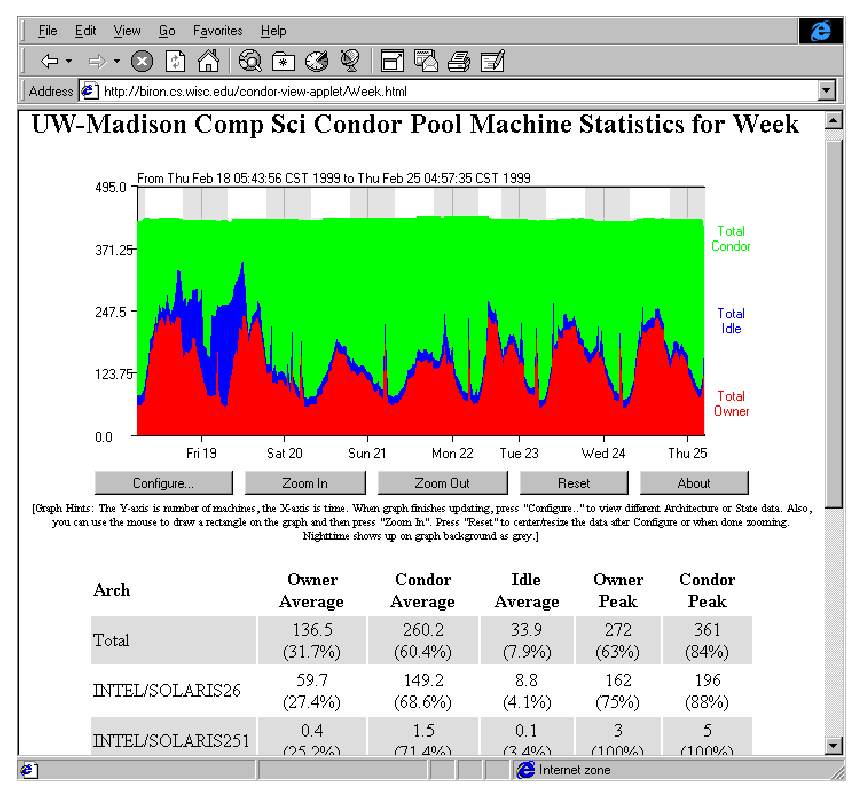
\includegraphics{admin-man/view-screenshot.ps}
\caption{\label{fig:view-screenshot}Screen shot of CondorView Client}
\end{figure}

After unpacking and installing the CondorView Client, a script named
\Prog{make\_stats} can be invoked to create HTML pages displaying Condor usage
for the past hour, day, week, or month.  
By using the Unix \Prog{cron} facility to periodically execute
\Prog{make\_stats}, Condor pool usage statistics can be kept up to date
automatically.  
This simple model allows the CondorView Client to be easily installed;
no Web server CGI interface is needed.

%%%%%%%%%%%%%%%%%%%%%%%%%%%%%%%%%%%%%%%%%%%%%%%%%%%%%%%%%%%%%%%%%%%%%%
\subsubsection{\label{sec:condorview-client-step-by-step}
Step-by-Step Installation of the CondorView Client}
%%%%%%%%%%%%%%%%%%%%%%%%%%%%%%%%%%%%%%%%%%%%%%%%%%%%%%%%%%%%%%%%%%%%%%

\index{installation!CondorView Client}
\index{CondorView!Client installation}
\begin{enumerate}

\item Make certain that the CondorView Server is configured.
Section ~\ref{sec:Contrib-CondorView-Install}
describes configuration of the server.
The server logs information on disk in order to provide a persistent,
historical database of pool statistics.
The CondorView Client makes queries over the network to this
database.
The \Condor{collector} includes this database support.
To activate the persistent database logging, add the following entries to
the configuration file for the \Condor{collector} chosen to act as the ViewServer.
\begin{verbatim}
    POOL_HISTORY_DIR = /full/path/to/directory/to/store/historical/data 
    KEEP_POOL_HISTORY = True 
\end{verbatim}

\item Create a directory where CondorView is to place the HTML files.  
This directory should be one published by a web server, so that HTML
files which exist in this directory can be accessed using a web browser.  
This directory is referred to as the \File{VIEWDIR} directory.

\item Download the \Prog{view\_client} contrib module.
Follow links for contrib modules on the downloads page at
\URL{http://www.cs.wisc.edu/condor/downloads-v2/download.pl}.

\item Unpack or untar this contrib module into the
directory \File{VIEWDIR}.
This creates several files and subdirectories.
Further unpack the jar file within the \File{VIEWDIR} directory with:
\begin{verbatim} 
  jar -xf condorview.jar
\end{verbatim}

\item Edit the \Prog{make\_stats} script.  At the beginning of the file
are six parameters to customize.
The parameters are

        \begin{description}

	\item[\MacroNI{ORGNAME}] A brief name that identifies an
	organization. An example is ``Univ of Wisconsin''.  Do not
	use any slashes in the name or other special regular-expression
	characters. Avoid the characters \Bs \^\  and \$.

	\item[\MacroNI{CONDORADMIN}] The e-mail
	address of the Condor administrator at your site.  
	This e-mail address will appear at the bottom of the web pages.

	\item[\MacroNI{VIEWDIR}] The full path name
	(\emph{not} a relative path) to the \File{VIEWDIR} directory set
	by installation step 2.  
	It is the directory that contains the \Prog{make\_stats} script.

	\item[\MacroNI{STATSDIR}]  The full path name of the
	directory which contains the \Condor{stats} binary.
	The \Condor{stats} program is included in the \Release{bin}
	directory. 
	The value for \MacroNI{STATSDIR} is added to the \MacroNI{PATH}
	parameter by default.  

	\item[\MacroNI{PATH}] A list of subdirectories,
	separated by colons, where the \Prog{make\_stats} script can find
	the \Prog{awk}, \Prog{bc}, \Prog{sed}, \Prog{date}, and \Condor{stats}
	programs.  
	If \Prog{perl} is installed, the path should also
	include the directory where \Prog{perl} is installed.
	The following default works on most systems:
        \begin{verbatim} 
        PATH=/bin:/usr/bin:$STATSDIR:/usr/local/bin
        \end{verbatim}

        \end{description}

\item To create all of the initial HTML files, run
\begin{verbatim}
        ./make_stats setup  
\end{verbatim}
Open the file \File{index.html} to verify that things look good.

\index{CondorView!use of \Prog{crontab} program}
\index{crontab program}

\item Add the \Prog{make\_stats} program to \Prog{cron}.  
Running \Prog{make\_stats} in step 6 created a \File{cronentries} file.
This \File{cronentries} file is ready to be processed by the Unix
\Prog{crontab} command.
The \Prog{crontab} manual page contains details about
the \Prog{crontab} command and the \Prog{cron} daemon.
Look at the
\File{cronentries} file; by default, it will run 
\Prog{make\_stats} \Arg{hour} every 15 minutes, 
\Prog{make\_stats} \Arg{day} once an hour, 
\Prog{make\_stats} \Arg{week} twice per day, and 
\Prog{make\_stats} \Arg{month} once per day.
These are reasonable defaults.  
Add these commands to cron on any
system that can access the \MacroNI{VIEWDIR} and
\MacroNI{STATSDIR} directories,
even on a system that does not have Condor installed.
The commands do not need to run as root user;
in fact, they should probably not run as root.  These commands can run
as any user that has read/write access to the \File{VIEWDIR} directory.
The command
\begin{verbatim} 
  crontab cronentries
\end{verbatim}
can set the crontab file;
note that this command overwrites the current, existing crontab file with the 
entries from the file \File{cronentries}.

\item Point the web browser at the \File{VIEWDIR} directory
to complete the installation.

\end{enumerate}


%%%%%%%%%%%%%%%%%%%%%%%%%%%%%%%%%%%%%%%%%%%%%%%%%%%%%%%%%%%%%%%%%%%%%%
%%%%%%%%%%%%%%%%%%%%%%%%%%%%%%%%%%%%%%%%%%%%%%%%%%%%%%%%%%%%%%%%%%%%%%%%%%%%%%%%
\subsection{\label{sec:Dynamic-Deployment}Dynamic Deployment}
%%%%%%%%%%%%%%%%%%%%%%%%%%%%%%%%%%%%%%%%%%%%%%%%%%%%%%%%%%%%%%%%%%%%%%%%%%%%%%%%
\index{dynamic deployment}
\index{deployment commands}

Dynamic deployment is a mechanism that allows rapid, automated
installation and start up of Condor resources on a given machine.
In this way any machine can be added to a Condor pool.
The dynamic
deployment tool set also provides tools to remove a machine from the
pool, without leaving residual effects on the machine such as leftover
installations, log files, and working directories.

\index{Condor commands!condor\_cold\_start}
Installation and start up is provided by \Condor{cold\_start}.
The \Condor{cold\_start} program determines the operating system and
architecture of the target machine, and transfers the correct
installation package from an ftp, http, or grid ftp site.
After transfer, it
installs Condor and creates a local working
directory for Condor to run in.  As a last step, \Condor{cold\_start}
begins running Condor in a manner which allows for later easy and reliable
shut down.

\index{Condor commands!condor\_cold\_stop}
The program that reliably shuts down and uninstalls a previously
dynamically installed Condor instance is \Condor{cold\_stop}.
\Condor{cold\_stop} begins by safely and reliably shutting off the
running Condor installation.  It ensures that Condor has
completely shut down before continuing, and optionally ensures that
there are no queued jobs at the site.
Next, \Condor{cold\_stop}
removes and optionally archives the Condor working directories,
including the \File{log} directory. 
These archives can be stored to a
mounted file system or to a grid ftp site.
As a last step,
\Condor{cold\_stop} uninstalls the Condor executables and libraries.
The end result is that the machine resources are left unchanged after
a dynamic deployment of Condor leaves.

%%%%%%%%%%%%%%%%%%%%%%%%%%%%%%%%%%%%%%%%%%%%%%%%%%%%%%%%%%%%%%%%%%%%%%%%%%%%%%%%
\subsubsection{Configuration and Usage}
%%%%%%%%%%%%%%%%%%%%%%%%%%%%%%%%%%%%%%%%%%%%%%%%%%%%%%%%%%%%%%%%%%%%%%%%%%%%%%%%

\index{dynamic deployment!configuration}
Dynamic deployment is designed for the expert Condor user
and administrator.
Tool design choices were made for functionality,
not ease-of-use.

Like every installation of Condor, a dynamically deployed installation
relies on a configuration.
To add a target
machine to a previously created Condor pool,
the global configuration file for that pool is a good starting point.
Modifications to that configuration can be made in a separate, 
local configuration file used in the dynamic deployment.
The global configuration file must
be placed on an ftp, http, grid ftp, or file server 
accessible by \Condor{cold\_start}.  The local configuration file
is to be on a file system accessible by the target machine.
There are some specific configuration variables that may be set for
dynamic deployment.  
A list of executables and directories which must be present
for Condor to start on the target machine may be set with
the configuration variables \Macro{DEPLOYMENT\_REQUIRED\_EXECS} and
\Macro{DEPLOYMENT\_REQUIRED\_DIRS}. 
If defined and the comma-separated list of executables or directories are
not present, then \Condor{cold\_start} exits with error.
Note this does not affect what is installed, only
whether start up is successful. 

A list of executables and directories which are recommended to be present
for Condor to start on the target machine may be set with
the configuration variables \Macro{DEPLOYMENT\_RECOMMENDED\_EXECS} and
\Macro{DEPLOYMENT\_RECOMMENDED\_DIRS}. 
If defined and the comma-separated lists of executables or directories are
not present, then \Condor{cold\_start} prints a warning message
and continues.
Here is a portion of the configuration relevant to
a dynamic deployment of a Condor submit node:

\footnotesize
\begin{verbatim}
DEPLOYMENT_REQUIRED_EXECS    = MASTER, SCHEDD, PREEN, STARTER, \
                               STARTER_STANDARD, SHADOW, \
                               SHADOW_STANDARD, GRIDMANAGER, GAHP, CONDOR_GAHP
DEPLOYMENT_REQUIRED_DIRS     = SPOOL, LOG, EXECUTE
DEPLOYMENT_RECOMMENDED_EXECS = CREDD
DEPLOYMENT_RECOMMENDED_DIRS  = LIB, LIBEXEC
\end{verbatim}
\normalsize

Additionally, the user must
specify which Condor services will be started.  This is done through
the \MacroNI{DAEMON\_LIST} configuration variable.  Another excerpt
from a dynamic submit node deployment configuration:

\footnotesize
\begin{verbatim}
DAEMON_LIST  = MASTER, SCHEDD
\end{verbatim}
\normalsize

Finally, the location
of the dynamically installed Condor executables is tricky to set,
since the location is unknown before installation.
Therefore,
the variable \Macro{DEPLOYMENT\_RELEASE\_DIR} is defined in the environment.
It corresponds to the location of the dynamic Condor installation.
If, as is often the case, 
the configuration file specifies the location of Condor executables in
relation to the \MacroNI{RELEASE\_DIR} variable, the configuration can
be made dynamically deployable by setting \MacroNI{RELEASE\_DIR} to
\MacroNI{DEPLOYMENT\_RELEASE\_DIR} as 

\footnotesize
\begin{verbatim}
RELEASE_DIR = $(DEPLOYMENT_RELEASE_DIR)
\end{verbatim}
\normalsize

In addition to setting up the configuration, the user must also
determine where the installation package will reside.
The installation package can be in either tar or 
gzipped tar form, and may
reside on a ftp, http, grid ftp, or file server.  
Create this installation package by tar'ing up the binaries and libraries
needed, and place them on the appropriate server.
The binaries can be tar'ed in a flat structure or within \File{bin} and
\File{sbin}.  Here is a list of files to give an example
structure for a dynamic deployment of the \Condor{schedd} daemon.

\footnotesize
\begin{verbatim}
% tar tfz latest-i686-Linux-2.4.21-37.ELsmp.tar.gz
bin/
bin/condor_config_val
bin/condor_q
sbin/
sbin/condor_preen
sbin/condor_shadow.std
sbin/condor_starter.std
sbin/condor_schedd
sbin/condor_master
sbin/condor_gridmanager
sbin/gt4_gahp
sbin/gahp_server
sbin/condor_starter
sbin/condor_shadow
sbin/condor_c-gahp
sbin/condor_off 
\end{verbatim}
\normalsize

%%%%%%%%%%%%%%%%%%%%%%%%%%%%%%%%%%%%%%%%%%%%%%%%%%%%%%%%%%%%%%%%%%%%%%

%%%%%%%%%%%%%%%%%%%%%%%%%%%%%%%%%%%%%%%%%%%%%%%%%%%%%%%%%%%%%%%%%%%%%%
\section{\label{sec:Configuring-Condor}Configuration}
%%%%%%%%%%%%%%%%%%%%%%%%%%%%%%%%%%%%%%%%%%%%%%%%%%%%%%%%%%%%%%%%%%%%%%

\index{Condor!configuration}
\index{configuration}

This section describes how to configure all parts of the Condor
system.  General information about the configuration
files and their syntax is followed by a description of
settings that affect all
Condor daemons and tools.
The 
settings that control the policy under which Condor will start,
suspend, resume, vacate or kill jobs
are described in 
section~\ref{sec:Configuring-Policy} on Startd Policy Configuration. 

%%%%%%%%%%%%%%%%%%%%%%%%%%%%%%%%%%%%%%%%%%%%%%%%%%%%%%%%%%%%%%%%%%%%%%
\subsection{\label{sec:Intro-to-Config-Files}Introduction to
Configuration Files} 
%%%%%%%%%%%%%%%%%%%%%%%%%%%%%%%%%%%%%%%%%%%%%%%%%%%%%%%%%%%%%%%%%%%%%%

The Condor configuration files are used to customize how Condor
operates at a given site.  The basic configuration as shipped with
Condor works well for most sites.

Each Condor program will, as part of its initialization process,
configure itself by calling a library routine which parses the
various configuration files that might be used including pool-wide,
platform-specific, and machine-specific configuration files.
Environment variables may also contribute to the configuration.

The result of configuration is a list of key/value pairs.
Each key is a configuration variable name,
and each value is a string literal
that may utilize macro substitution (as defined below).
Some configuration variables are evaluated by Condor as ClassAd
expressions; some are not.  Consult the documentation for each specific
case.  Unless otherwise noted, configuration values that are expected
to be numeric or boolean constants may be any valid ClassAd expression
of operators on constants.  Example:

\begin{verbatim}
MINUTE          = 60
HOUR            = (60 * $(MINUTE))
SHUTDOWN_GRACEFUL_TIMEOUT = ($(HOUR)*24)
\end{verbatim}

%%%%%%%%%%%%%%%%%%%%%%%%%%%%%%%%%%%%%%%%%%%%%%%%%%%%%%%%%%%%%%%%%%%%%%
\subsubsection{\label{sec:Ordering-Config-File}Ordered Evaluation to
Set the Configuration} 
%%%%%%%%%%%%%%%%%%%%%%%%%%%%%%%%%%%%%%%%%%%%%%%%%%%%%%%%%%%%%%%%%%%%%%
\index{configuration file!evaluation order}

Multiple files, as well as a program's environment variables
determine the configuration.
The order in which attributes are defined is important, as later
definitions override existing definitions.
The order in which the (multiple) configuration files are parsed 
is designed to ensure the security of the system.
Attributes which must be set a specific way 
must appear in the last file to be parsed.
This prevents both the naive and the malicious Condor user 
from subverting the system through its configuration.
The order in which items are parsed is
\begin{enumerate}
\item global configuration file
\item local configuration file
\item specific environment variables prefixed with \MacroNI{\_CONDOR\_}
\end{enumerate}

The locations for these files are as given in
section~\ref{sec:Config-File-Locations} on
page~\pageref{sec:Config-File-Locations}.

Some Condor tools utilize environment variables to set their
configuration.
These tools search for specifically-named environment variables.
The variables are prefixed by the string \MacroNI{\_CONDOR\_}
or \MacroNI{\_condor\_}.
The tools strip off the prefix, and utilize what remains
as configuration.
As the use of environment variables is the last within
the ordered evaluation, 
the environment variable definition is used.
The security of the system is not compromised,
as only specific variables are considered for definition
in this manner, not any environment variables with
the \MacroNI{\_CONDOR\_} prefix.


%%%%%%%%%%%%%%%%%%%%%%%%%%%%%%%%%%%%%%%%%%%%%%%%%%%%%%%%%%%%%%%%%%%%%%
\subsubsection{\label{sec:Config-File-Macros}Configuration File Macros} 
%%%%%%%%%%%%%%%%%%%%%%%%%%%%%%%%%%%%%%%%%%%%%%%%%%%%%%%%%%%%%%%%%%%%%%

\index{macro!in configuration file}
\index{configuration file!macro definitions}

Macro definitions are of the form:
\begin{verbatim}
<macro_name> = <macro_definition>
\end{verbatim}

The macro name given on the left hand side of the definition is
a case sensitive identifier.
There must be white space between the macro name, the
equals sign (\verb@=@), and the macro definition.
The macro definition is a string literal that may utilize macro substitution.

Macro invocations are of the form: 
\begin{verbatim}
$(macro_name)
\end{verbatim}

Macro definitions may contain references to other macros, even ones
that are not yet defined, as long as they are eventually defined in
the configuration files.
All macro expansion is done after all configuration files have been parsed,
with the exception of macros that reference themselves.

\begin{verbatim}
A = xxx
C = $(A) 
\end{verbatim}
is a legal set of macro definitions, and the resulting value of 
\MacroNI{C} is
\Expr{xxx}.
Note that
\MacroNI{C} is actually bound to 
\MacroUNI{A}, not its value.

As a further example,
\begin{verbatim}
A = xxx
C = $(A)
A = yyy
\end{verbatim}
is also a legal set of macro definitions, and the resulting value of
\MacroNI{C} is \Expr{yyy}.  

A macro may be incrementally defined by invoking itself in its
definition.  For example,
\begin{verbatim}
A = xxx
B = $(A)
A = $(A)yyy
A = $(A)zzz
\end{verbatim}
is a legal set of macro definitions, and the resulting value of 
\MacroNI{A}
is \Expr{xxxyyyzzz}.
Note that invocations of a macro in
its own definition are immediately
expanded.
\MacroUNI{A} is immediately expanded in line 3 of the example.
If it were not, then the definition would be impossible to
evaluate.

Recursively defined macros such as
\begin{verbatim}
A = $(B)
B = $(A)
\end{verbatim}
are not allowed.
They create definitions that Condor refuses to parse. 

All entries in a configuration file must have an operator,
which will be an equals sign (\verb@=@).
Identifiers are alphanumerics combined with the underscore character,
optionally with a subsystem name and a period as a prefix.
As a special case,
a line without an operator that begins with a left square bracket
will be ignored.
The following two-line example treats the first line as a comment,
and correctly handles the second line.
\begin{verbatim}
[Condor Settings]
my_classad = [ foo=bar ]
\end{verbatim}

% functionality added to version 6.7.13
To simplify pool administration,
any configuration variable name may be prefixed by
a subsystem 
(see the \MacroUNI{SUBSYSTEM} macro in 
section~\ref{sec:Pre-Defined-Macros}
for the list of subsystems)
and the period (\verb@.@) character.
For configuration variables defined this way,
the value is applied to the specific subsystem.
For example,
the ports that Condor may use can be restricted to a range 
using the \MacroNI{HIGHPORT} and \MacroNI{LOWPORT} configuration
variables.
If the range of intended ports is different for specific
daemons, this syntax may be used.

\begin{verbatim}
  MASTER.LOWPORT   = 20000
  MASTER.HIGHPORT  = 20100
  NEGOTIATOR.LOWPORT   =  22000 
  NEGOTIATOR.HIGHPORT  =  22100
\end{verbatim}

Note that all configuration variables may utilize this syntax,
but nonsense configuration variables may result.
For example, it makes no sense to define
\begin{verbatim}
  NEGOTIATOR.MASTER_UPDATE_INTERVAL = 60
\end{verbatim}
since the \Condor{negotiator} daemon does not use the
\MacroNI{MASTER\_UPDATE\_INTERVAL} variable.

It makes little sense to do so, but Condor will configure
correctly with a definition such as
\begin{verbatim}
  MASTER.MASTER_UPDATE_INTERVAL = 60
\end{verbatim}
The \Condor{master} uses this configuration variable,
and the prefix of \MacroNI{MASTER.} causes this configuration
to be specific to the \Condor{master} daemon.

% the local functionality added in 7.1.4
This syntax has been further expanded to allow for the
specification of a local name on the command line 
using the command line option
\begin{verbatim}
  -local-name <local-name>
\end{verbatim}
This allows multiple instances of a daemon to be run 
by the same \Condor{master} daemon,
each instance with its own local configuration variable.

The ordering used to look up a variable, called \verb@<parameter name>@:

\begin{enumerate}
\item \verb@<subsystem name>.<local name>.<parameter name>@

\item \verb@<local name>.<parameter name>@

\item \verb@<subsystem name>.<parameter name>@

\item \verb@<parameter name>@
\end{enumerate}

If this local name is not specified on the command line, 
numbers 1 and 2 are skipped.
As soon as the first match is found, the search is completed,
and the corresponding value is used.

This example configures a \Condor{master} to run 2 \Condor{schedd}
daemons.  The \Condor{master} daemon needs the configuration:
\begin{verbatim}
  XYZZY           = $(SCHEDD)
  XYZZY_ARGS      = -local-name xyzzy
  DAEMON_LIST     = $(DAEMON_LIST) XYZZY
  DC_DAEMON_LIST  = + XYZZY
  XYZZY_LOG       = $(LOG)/SchedLog.xyzzy
\end{verbatim}

Using this example configuration, the \Condor{master} starts up a
second \Condor{schedd} daemon, 
where this second \Condor{schedd} daemon is passed 
\OptArg{-local-name}{xyzzy}
on the command line.

Continuing the example,
configure the \Condor{schedd} daemon named \Attr{xyzzy}.
This \Condor{schedd} daemon will share all configuration variable
definitions with the other \Condor{schedd} daemon,
except for those specified separately.

\begin{verbatim}
  SCHEDD.XYZZY.SCHEDD_NAME = XYZZY
  SCHEDD.XYZZY.SCHEDD_LOG  = $(XYZZY_LOG)
  SCHEDD.XYZZY.SPOOL       = $(SPOOL).XYZZY
\end{verbatim}

Note that the example \MacroNI{SCHEDD\_NAME} and \MacroNI{SPOOL} are
specific to the \Condor{schedd} daemon, as opposed to a different daemon
such as the \Condor{startd}.
Other Condor daemons using this feature will
have different requirements for which parameters need to be
specified individually.  This example works for the \Condor{schedd},
and more local configuration can, and likely would be specified.

Also note that each daemon's log file must be specified individually,
and in two places: one specification is for use by the \Condor{master},
and the other is for use by the daemon itself.
In the example,
the \Attr{XYZZY} \Condor{schedd} configuration variable
\MacroNI{SCHEDD.XYZZY.SCHEDD\_LOG} definition references the
\Condor{master} daemon's \MacroNI{XYZZY\_LOG}.


%%%%%%%%%%%%%%%%%%%%%%%%%%%%%%%%%%%%%%%%%%%%%%%%%%%%%%%%%%%%%%%%%%%%%%
\subsubsection{\label{sec:Other-Syntax}Comments and Line Continuations}
%%%%%%%%%%%%%%%%%%%%%%%%%%%%%%%%%%%%%%%%%%%%%%%%%%%%%%%%%%%%%%%%%%%%%%

A Condor configuration file may contain comments and
line continuations.
A comment is any line beginning with a pound character (\verb@#@).
A continuation is any entry that continues across multiples lines.
Line continuation is accomplished by placing the backslash
character (\Bs) at the end of any line to be continued onto another.
Valid examples of line continuation are
\begin{verbatim}
  START = (KeyboardIdle > 15 * $(MINUTE)) && \
  ((LoadAvg - CondorLoadAvg) <= 0.3)
\end{verbatim}
and
\begin{verbatim}
  ADMIN_MACHINES = condor.cs.wisc.edu, raven.cs.wisc.edu, \
  stork.cs.wisc.edu, ostrich.cs.wisc.edu, \
  bigbird.cs.wisc.edu
  HOSTALLOW_ADMIN = $(ADMIN_MACHINES)
\end{verbatim}

Note that a line continuation character may currently be used within
a comment, so the following example does \emph{not} set the
configuration variable \MacroNI{FOO}:
\begin{verbatim}
  # This comment includes the following line, so FOO is NOT set \
  FOO = BAR
\end{verbatim}
It is a poor idea to use this functionality, as it is likely to
stop working in future Condor releases.

%%%%%%%%%%%%%%%%%%%%%%%%%%%%%%%%%%%%%%%%%%%%%%%%%%%%%%%%%%%%%%%%%%%%%%
\subsubsection{\label{sec:Program-Defined-Macros}Executing a Program to Produce Configuration Macros}
%%%%%%%%%%%%%%%%%%%%%%%%%%%%%%%%%%%%%%%%%%%%%%%%%%%%%%%%%%%%%%%%%%%%%%

Instead of reading from a file,
Condor may run a program to obtain configuration macros.
The vertical bar character (\Bar) as the last character defining
a file name provides the syntax necessary to tell 
Condor to run a program.
This syntax may only be used in the definition of
the \Env{CONDOR\_CONFIG} environment variable,
or the \Macro{LOCAL\_CONFIG\_FILE} configuration variable.

The command line for the program 
is formed by the characters preceding the vertical bar character.
The standard output of the program is parsed as a configuration 
file would be.

An example:
\begin{verbatim}
LOCAL_CONFIG_FILE = /bin/make_the_config|
\end{verbatim}

Program \Prog{/bin/make\_the\_config} is executed, and its output
is the set of configuration macros.

Note that either a program is executed to generate the
configuration macros or the configuration is read from 
one or more files.
The syntax uses space characters to separate command line elements,
if an executed program produces the configuration macros.
Space characters would otherwise separate the list of files.
This syntax does not permit distinguishing one from the other,
so only one may be specified.

%%%%%%%%%%%%%%%%%%%%%%%%%%%%%%%%%%%%%%%%%%%%%%%%%%%%%%%%%%%%%%%%%%%%%%
\subsubsection{\label{sec:Macros-Requiring-Restart}Macros That Will Require a Restart When Changed}
%%%%%%%%%%%%%%%%%%%%%%%%%%%%%%%%%%%%%%%%%%%%%%%%%%%%%%%%%%%%%%%%%%%%%%
\index{configuration change requiring a restart of Condor}
When any of the following listed configuration variables are changed,
Condor must be restarted.
Reconfiguration using \Condor{reconfig} will not be enough.

\begin{itemize}
  \item \verb@BIND_ALL_INTERFACES@
  \item \verb@FetchWorkDelay@
  \item \verb@MAX_NUM_CPUS@
  \item \verb@MAX_TRACKING_GID@
  \item \verb@MIN_TRACKING_GID@
  \item \verb@NETWORK_INTERFACE@
  \item \verb@NUM_CPUS@
  \item \verb@PREEMPTION_REQUIREMENTS_STABLE@
  \item \verb@PRIVSEP_ENABLED@
  \item \verb@PROCD_ADDRESS@
\end{itemize}

%%%%%%%%%%%%%%%%%%%%%%%%%%%%%%%%%%%%%%%%%%%%%%%%%%%%%%%%%%%%%%%%%%%%%%
\subsubsection{\label{sec:Pre-Defined-Macros}Pre-Defined Macros}
%%%%%%%%%%%%%%%%%%%%%%%%%%%%%%%%%%%%%%%%%%%%%%%%%%%%%%%%%%%%%%%%%%%%%%

\index{configuration!pre-defined macros}
\index{configuration file!pre-defined macros}
Condor provides pre-defined macros that help configure Condor.
Pre-defined macros are listed as \MacroUNI{macro\_name}.

This first set are entries whose values are determined at
run time and cannot be overwritten.  These are inserted automatically by
the library routine which parses the configuration files.
This implies that a change to the underlying value of any of these
variables will require a full restart of Condor in order to use
the changed value.
\begin{description}
  
\label{param:FullHostname}
\item[\MacroU{FULL\_HOSTNAME}]
  The fully qualified host name of the local machine, 
  which is host name plus domain name.
  
\label{param:Hostname}
\item[\MacroU{HOSTNAME}]
  The host name of the local machine (no domain name).
  
\label{param:IpAddress}
\item[\MacroU{IP\_ADDRESS}]
  The ASCII string version of the local machine's IP address.

\label{param:Tilde}
\item[\MacroU{TILDE}]
  The full path to the
  home directory of the Unix user condor, if such a user exists on the
  local machine.

  \label{sec:Condor-Subsystem-Names}
  \index{configuration file!subsystem names}
\label{param:Subsystem}
\item[\MacroU{SUBSYSTEM}]
  The subsystem
  name of the daemon or tool that is evaluating the macro.
  This is a unique string which identifies a given daemon within the
  Condor system.  The possible subsystem names are:

  \index{subsystem names}
  \index{macro!subsystem names}
  \begin{itemize}
  \label{list:subsystem names}
  \item \verb@C_GAHP@
  \item \verb@CKPT_SERVER@
  \item \verb@COLLECTOR@
  \item \verb@DBMSD@
  \item \verb@DEFRAG@
  \item \verb@EC2_GAHP@
  \item \verb@GRIDMANAGER@
  \item \verb@HAD@
  \item \verb@HDFS@
  \item \verb@JOB_ROUTER@
  \item \verb@KBDD@ 
  \item \verb@LEASEMANAGER@
  \item \verb@MASTER@
  \item \verb@NEGOTIATOR@
  \item \verb@QUILL@
  \item \verb@REPLICATION@
  \item \verb@ROOSTER@
  \item \verb@SCHEDD@
  \item \verb@SHADOW@
  \item \verb@STARTD@
  \item \verb@STARTER@
  %\item \verb@STORK@
  \item \verb@SUBMIT@
  \item \verb@TOOL@
  \item \verb@TRANSFERER@
  \end{itemize}

\end{description}

This second set of macros are entries whose default values are
determined automatically at run time but which can be overwritten.  
\index{configuration file!macros}
\begin{description}

\label{param:Arch}
\item[\MacroU{ARCH}]
  Defines the string
  used to identify the architecture of the local machine to Condor.
  The \Condor{startd} will advertise itself with this attribute so
  that users can submit binaries compiled for a given platform and
  force them to run on the correct machines.  \Condor{submit} will
  append a requirement to the job ClassAd that it must
  run on the same \MacroNI{ARCH} and \MacroNI{OPSYS} of the machine where
  it was submitted, unless the user specifies \MacroNI{ARCH} and/or
  \MacroNI{OPSYS} explicitly in their submit file.  See the
  the \Condor{submit} manual page
  on page~\pageref{man-condor-submit} for details.

\label{param:OpSys}
\item[\MacroU{OPSYS}]
  Defines the string used to identify the operating system
  of the local machine to Condor.
  If it is not defined in the configuration file, Condor will
  automatically insert the operating system of this machine as
  determined by \Prog{uname}.

\label{param:OpSysVer}
\item[\MacroU{OPSYS\_VER}]
  Defines the integer used to identify the operating system version number.

\label{param:OpSysAndVer}
\item[\MacroU{OPSYS\_AND\_VER}]
  Defines the string used prior to Condor version 7.7.2 as \MacroUNI{OPSYS}.

\label{param:UnameArch}
\item[\MacroU{UNAME\_ARCH}]
  The architecture as reported by \Prog{uname}(2)'s \Code{machine} field.
  Always the same as \MacroNI{ARCH} on Windows.

\label{param:UnameOpsys}
\item[\MacroU{UNAME\_OPSYS}]
  The operating system as reported by \Prog{uname}(2)'s \Code{sysname} field.
  Always the same as \MacroNI{OPSYS} on Windows.

\label{param:DetectedMemory}
\item[\MacroU{DETECTED\_MEMORY}]
  The amount of detected physical memory (RAM) in Mbytes.

\label{param:DetectedCores}
\item[\MacroU{DETECTED\_CORES}]
  The number of detected CPU cores.  
  This includes hyper threaded cores, if there are any.

\label{param:Pid}
\item[\MacroU{PID}]
  The process ID for the daemon or tool.

\label{param:Ppid}
\item[\MacroU{PPID}]
  The process ID of the parent process for the daemon or tool.

\label{param:Username}
\item[\MacroU{USERNAME}]
  The user name of the UID of the daemon or tool.
  For daemons started as root, but running under another UID
  (typically the user condor), this will be the other UID.

\label{param:FilesystemDomain}
\item[\MacroU{FILESYSTEM\_DOMAIN}]
  Defaults to the fully
  qualified host name of the machine it is evaluated on.  See
  section~\ref{sec:Shared-Filesystem-Config-File-Entries}, Shared
  File System Configuration File Entries for the full description of
  its use and under what conditions you would want to change it.

\label{param:UIDDomain}
\item[\MacroU{UID\_DOMAIN}]
  Defaults to the fully
  qualified host name of the machine it is evaluated on.  See
  section~\ref{sec:Shared-Filesystem-Config-File-Entries} 
  for the full description of this configuration variable.

\end{description}

Since \MacroUNI{ARCH} and \MacroUNI{OPSYS} will automatically be set to the
correct values, we recommend that you do not overwrite them.
Only do so if you know what you are doing.



%%%%%%%%%%%%%%%%%%%%%%%%%%%%%%%%%%%%%%%%%%%%%%%%%%%%%%%%%%%%%%%%%%%%%%
\subsection{\label{sec:Config-File-Special}Special Macros}
%%%%%%%%%%%%%%%%%%%%%%%%%%%%%%%%%%%%%%%%%%%%%%%%%%%%%%%%%%%%%%%%%%%%%%

\index{configuration file!\$ENV definition}
\index{\$ENV!in configuration file}
References to the Condor process's environment are allowed in the
configuration files.
Environment references use the \Macro{ENV} macro and are of the form:
\begin{verbatim}
  $ENV(environment_variable_name)
\end{verbatim}
For example, 
\begin{verbatim}
  A = $ENV(HOME)
\end{verbatim}
binds \MacroNI{A} to the value of the HOME environment variable.
Environment references are not currently used in standard Condor
configurations.
However, they can sometimes be useful in custom configurations.

\index{\$RANDOM\_CHOICE()!in configuration}
This same syntax is used in the \Macro{RANDOM\_CHOICE()} macro to
allow a random choice of a parameter
within a configuration file.
These references are of the form:
\begin{verbatim}
  $RANDOM_CHOICE(list of parameters)
\end{verbatim}
This allows a random choice within the parameter list to be made
at configuration time.  Of the list of parameters, one is
chosen when encountered during configuration.  For example,
if one of the integers 0-8 (inclusive) should be randomly
chosen, the macro usage is
\begin{verbatim}
  $RANDOM_CHOICE(0,1,2,3,4,5,6,7,8)
\end{verbatim}

\index{\$RANDOM\_INTEGER()!in configuration}
The \Macro{RANDOM\_INTEGER()} macro is similar to the \MacroNI{RANDOM\_CHOICE()}
macro, and is used to select a random integer within a configuration file.
References are of the form:
\begin{verbatim}
  $RANDOM_INTEGER(min, max [, step])
\end{verbatim}
A random integer within the range \verb@min@ and \verb@max@, inclusive,
is selected at configuration time.
The optional \verb@step@ parameter
controls the stride within the range, and it defaults to the value 1.
For example, to randomly chose an even integer in the range 0-8 (inclusive),
the macro usage is
\begin{verbatim}
  $RANDOM_INTEGER(0, 8, 2)
\end{verbatim}

See section~\ref{sec:randomintegerusage} on
page~\pageref{sec:randomintegerusage}
for an actual use of this specialized macro.
%%%%%%%%%%%%%%%%%%%%%%%%%%%%%%%%%%%%%%%%%%%%%%%%%%%%%%%%%%%%%%%%%%%%%%
\subsection{\label{sec:Condor-wide-Config-File-Entries}Condor-wide Configuration File Entries} 
%%%%%%%%%%%%%%%%%%%%%%%%%%%%%%%%%%%%%%%%%%%%%%%%%%%%%%%%%%%%%%%%%%%%%%

\index{configuration!Condor-wide configuration variables}

This section describes settings which affect all parts of the Condor
system. 
Other system-wide settings can be found in
section~\ref{sec:Network-Related-Config-File-Entries} on
``Network-Related Configuration File Entries'', and
section~\ref{sec:Shared-Filesystem-Config-File-Entries} on ``Shared
File System Configuration File Entries''. 

\begin{description}
  
\label{param:CondorHost}
\item[\Macro{CONDOR\_HOST}]
  This macro may be
  used to define the \MacroUNI{NEGOTIATOR\_HOST} and is used to define the
  \MacroUNI{COLLECTOR\_HOST} macro.  Normally the \Condor{collector}
  and \Condor{negotiator} would run on the same machine.  If for some
  reason they were not run on the same machine,
  \MacroUNI{CONDOR\_HOST} would not be needed.  Some
  of the host-based security macros use \MacroUNI{CONDOR\_HOST} by
  default.  See section~\ref{sec:Host-Security}, on Setting up
  IP/host-based security in Condor for details.
  
\label{param:CollectorHost}
\item[\Macro{COLLECTOR\_HOST}]
  The host name of the machine where the \Condor{collector} is running for
  your pool.  Normally, it is defined relative to
  the \MacroUNI{CONDOR\_HOST}
  macro.  There is no default value for this macro;
  \MacroNI{COLLECTOR\_HOST} must be defined for the pool to work
  properly.

  In addition to defining the host name, this setting can optionally be
  used to specify the network port of the \Condor{collector}.
  The port is separated from the host name by a colon ('\verb@:@').
  For example,
  \begin{verbatim}
    COLLECTOR_HOST = $(CONDOR_HOST):1234
  \end{verbatim}
  If no port is specified, the default port of 9618 is used.
  Using the default port is recommended for most sites.
  It is only changed if there is a conflict with another
  service listening on the same network port.
  For more information about specifying a non-standard port for the
  \Condor{collector} daemon,
  see section~\ref{sec:Ports-NonStandard} on
  page~\pageref{sec:Ports-NonStandard}.


\label{param:NegotiatorHost} 
\item[\Macro{NEGOTIATOR\_HOST}]
  This configuration variable is no longer used.
  It previously defined the host name of the machine where 
  the \Condor{negotiator} is running.
  At present, the port where the \Condor{negotiator} is listening 
  is dynamically allocated.

  % commented out by Karen in 2008, as this 6.7ism is too old
  %For pools running 6.7.3 and older versions: The
  %host name of the machine where the \Condor{negotiator} is running for
  %the pool.
  %Normally, it is defined relative to the \MacroUNI{CONDOR\_HOST}
  %macro.  There is no default value for this macro;
  %\MacroNI{NEGOTIATOR\_HOST} must be defined for the pool to work
  %properly.
  %This variable may also be used to optionally define a network port for
  %the \Condor{negotiator} daemon, as explained for the
  %\MacroNI{COLLECTOR\_HOST} variable.

\label{param:CondorViewHost}
\item[\Macro{CONDOR\_VIEW\_HOST}]
  A list of CondorView servers, separated by commas and/or spaces.
  Each CondorView server is denoted by the host name of the machine
  it is running on, optionally appended by a colon and the port number.
  This service is optional, and requires additional configuration 
  to enable it.  There is no default value for
  \MacroNI{CONDOR\_VIEW\_HOST}.  If \MacroNI{CONDOR\_VIEW\_HOST} is not
  defined, no CondorView server is used.
  See section~\ref{sec:Contrib-CondorView-Install} on
  page~\pageref{sec:Contrib-CondorView-Install} for more details.

\label{param:ScheddHost}
\item[\Macro{SCHEDD\_HOST}]
  The host name of the machine where the \Condor{schedd} is running for
  your pool.  This is the host that queues submitted jobs.
  If the host specifies \Macro{SCHEDD\_NAME} or \Macro{MASTER\_NAME}, that
  name must be included in the form name\verb$@$hostname.
  In most condor installations, there is a \Condor{schedd} running on
  each host from which jobs are submitted.  The default value of
  \Macro{SCHEDD\_HOST} is the current host with the optional name included.  For most pools, this
  macro is not defined, nor does it need to be defined..

\label{param:ReleaseDir}
\item[\Macro{RELEASE\_DIR}]
  The full path to
  the Condor release directory, which holds the \File{bin},
  \File{etc}, \File{lib}, and \File{sbin} directories.  Other macros
  are defined relative to this one.  There is no default value for
  \Macro{RELEASE\_DIR}.

\label{param:Bin}
\item[\Macro{BIN}]
  This directory points to the
  Condor directory where user-level programs are installed.  It is
  usually defined relative to the \MacroUNI{RELEASE\_DIR} macro.
  There is no default value for \Macro{BIN}.
  
\label{param:Lib}
\item[\Macro{LIB}]
  This directory points to the
  Condor directory where libraries used to link jobs for Condor's
  standard universe are stored.  The \Condor{compile} program uses
  this macro to find these libraries, so it must be defined for
  \Condor{compile} to function.  \MacroUNI{LIB} is usually defined
  relative to the \MacroUNI{RELEASE\_DIR} macro, and has no default
  value.

\label{param:LibExec}
\item[\Macro{LIBEXEC}]
  This directory points
  to the Condor directory where support commands that Condor
  needs will be placed.
  Do not add this directory to a user or system-wide path.

\label{param:Include}
\item[\Macro{INCLUDE}]
  This directory points to the Condor directory where header files reside.
  \MacroUNI{INCLUDE} would usually be defined relative to
  the \MacroUNI{RELEASE\_DIR} configuration macro.
  There is no default value, but
  if defined, it can make inclusion of necessary header files
  for compilation of programs (such as those programs
  that use \File{libcondorapi.a})
  easier through the use of \Condor{config\_val}.

\label{param:Sbin}
\item[\Macro{SBIN}]
  This directory points to the
  Condor directory where Condor's system binaries (such as the
  binaries for the Condor daemons) and administrative tools are
  installed.  Whatever directory \MacroU{SBIN} points to ought
  to be in the \Env{PATH} of users acting as Condor
  administrators.  \Macro{SBIN} has no default value.

\label{param:LocalDir}
\item[\Macro{LOCAL\_DIR}]
  The location of the
  local Condor directory on each machine in your pool.  One common
  option is to use the condor user's home directory which may be
  specified with \MacroUNI{TILDE}.  There is no default value for
  \Macro{LOCAL\_DIR}.  For example:
  \begin{verbatim}
    LOCAL_DIR = $(tilde)
  \end{verbatim}
  
  On machines with a shared file system, where either the
  \MacroUNI{TILDE} directory or another directory you want to use is
  shared among all machines in your pool, you might use the
  \MacroUNI{HOSTNAME} macro and have a directory with many
  subdirectories, one for each machine in your pool, each named by
  host names.  For example:
  \begin{verbatim}
    LOCAL_DIR = $(tilde)/hosts/$(hostname)      
  \end{verbatim}
  or:
  \begin{verbatim}
    LOCAL_DIR = $(release_dir)/hosts/$(hostname)
  \end{verbatim}
  
\label{param:Log}
\item[\Macro{LOG}]
  Used to specify the
  directory where each Condor daemon writes its log files.  The names
  of the log files themselves are defined with other macros, which use
  the \MacroUNI{LOG} macro by default.  The log directory also acts as
  the current working directory of the Condor daemons as the run, so
  if one of them should produce a core file for any reason, it would
  be placed in the directory defined by this macro.  \MacroNI{LOG} is
  required to be defined.  Normally, \MacroUNI{LOG} is defined in
  terms of \MacroUNI{LOCAL\_DIR}.
  
\label{param:Spool}
\item[\Macro{SPOOL}]
  The spool directory is where
  certain files used by the \Condor{schedd} are stored, such as the
  job queue file and the initial executables of any jobs that have
  been submitted.  In addition, for systems not using a checkpoint
  server, all the checkpoint files from jobs that have been submitted
  from a given machine will be store in that machine's spool
  directory.  Therefore, you will want to ensure that the spool
  directory is located on a partition with enough disk space.  If a
  given machine is only set up to execute Condor jobs and not submit
  them, it would not need a spool directory (or this macro defined).
  There is no default value for \Macro{SPOOL}, and the \Condor{schedd}
  will not function without it \Macro{SPOOL} defined.  Normally,
  \MacroUNI{SPOOL} is defined in terms of \MacroUNI{LOCAL\_DIR}.
  
\label{param:Execute}
\item[\Macro{EXECUTE}]
  This directory acts as
  a place to create the scratch directory of any Condor job that is executing
  on
  the local machine.  The scratch directory is the destination of
  any input files that were specified for transfer.  It also serves
  as the job's working directory if the job is using file transfer
  mode and no other working directory was specified.
  If a given machine is set up to only submit
  jobs and not execute them, it would not need an execute directory,
  and this macro need not be defined.  There is no default value for
  \MacroNI{EXECUTE}, and the \Condor{startd} will not function if
  \MacroNI{EXECUTE} is undefined.  Normally, \MacroUNI{EXECUTE} is
  defined in terms of \MacroUNI{LOCAL\_DIR}.  To customize the execute
  directory independently for each batch slot, use \MacroNI{SLOT<N>\_EXECUTE}.

\label{param:SlotNExecute}
\item[\Macro{SLOT<N>\_EXECUTE}]
  Specifies an
  execute directory for use by a specific batch slot.
  \MacroNI{<N>} represents the number of the batch slot, such as 1, 2, 3, etc.
  This execute directory serves the same purpose as \Macro{EXECUTE}, but it
  allows the configuration of the directory independently for each batch
  slot.  Having slots each using a different partition would be
  useful, for example, in preventing one job from filling up the same
  disk that other jobs are trying to write to.  If this parameter is
  undefined for a given batch slot, it will use \MacroNI{EXECUTE} as
  the default.  Note that each slot will advertise \AdAttr{TotalDisk}
  and \AdAttr{Disk} for the partition containing its execute
  directory.

\label{param:LocalConfigFile}
\item[\Macro{LOCAL\_CONFIG\_FILE}]
  Identifies the
  location of the local, machine-specific configuration
  file for each machine
  in the pool.  The two most common choices would be putting this
  file in the \MacroUNI{LOCAL\_DIR}, or putting all
  local configuration files for the pool in a shared directory, each one
  named by host name.  For example,
  \begin{verbatim}
    LOCAL_CONFIG_FILE = $(LOCAL_DIR)/condor_config.local
  \end{verbatim}
  or,
  \begin{verbatim}
    LOCAL_CONFIG_FILE = $(release_dir)/etc/$(hostname).local
  \end{verbatim}
  or, not using the release directory
  \begin{verbatim}
    LOCAL_CONFIG_FILE = /full/path/to/configs/$(hostname).local
  \end{verbatim}
  
  The value of \MacroNI{LOCAL\_CONFIG\_FILE} is treated as a list of files,
  not a
  single file.  The items in the list are delimited by either commas
  or space characters.
  This allows the specification of multiple files as
  the local configuration file, each one processed in the
  order given (with parameters set in later files overriding values
  from previous files).  This allows the use of one global
  configuration file for multiple platforms in the pool, defines a
  platform-specific configuration file for each platform, and uses a
  local configuration file for each machine. 
  If the list of files is changed in one of the later read files, the new list
  replaces the old list, but any files that have already been processed
  remain processed, and are removed from the new list if they are present
  to prevent cycles.
  See section~\ref{sec:Program-Defined-Macros} on 
  page~\pageref{sec:Program-Defined-Macros} for directions on
  using a program to generate the configuration macros that would
  otherwise reside in one or more files as described here.
  If \MacroNI{LOCAL\_CONFIG\_FILE} is not defined, no local configuration
  files are processed.  For more information on this, see
  section~\ref{sec:Multiple-Platforms} about Configuring Condor for
  Multiple Platforms on page~\pageref{sec:Multiple-Platforms}.

  If all files in a directory are local configuration files to be processed,
  then consider using \MacroNI{LOCAL\_CONFIG\_DIR}, defined at
  section~\ref{param:LocalConfigDir}.

\label{param:RequireLocalConfigFile}
\item[\Macro{REQUIRE\_LOCAL\_CONFIG\_FILE}]
  A boolean value that defaults to \Expr{True}.
  When \Expr{True}, Condor exits with an error,
  if any file listed in \MacroNI{LOCAL\_CONFIG\_FILE} cannot be read.
  A value of \Expr{False} allows local configuration files to be missing.
  This is most useful for sites that have 
  both large numbers of machines in the pool and a local configuration file
  that uses the \MacroUNI{HOSTNAME} macro in its definition.
  Instead of having an empty file for every host
  in the pool, files can simply be omitted.

\label{param:LocalConfigDir} 
\item[\Macro{LOCAL\_CONFIG\_DIR}]
  A directory may be used as a container for local configuration files. 
  The files found in the directory are sorted into lexicographical order 
  by file name, and 
  then each file is treated as though it was listed in 
  \MacroNI{LOCAL\_CONFIG\_FILE}. 
  \MacroNI{LOCAL\_CONFIG\_DIR} is processed before any files listed in 
  \MacroNI{LOCAL\_CONFIG\_FILE}, and is checked again after processing
  the \MacroNI{LOCAL\_CONFIG\_FILE} list. 
  It is a list of directories, and each directory is processed in the order
  it appears in the list. 
  The process is not recursive, so any directories found inside the directory
  being processed are ignored. 
  See also \MacroNI{LOCAL\_CONFIG\_DIR\_EXCLUDE\_REGEXP}.

\label{param:LocalConfigDirExcludeRegexp}
\item[\Macro{LOCAL\_CONFIG\_DIR\_EXCLUDE\_REGEXP}]
  A regular expression that specifies file names to be ignored when
  looking for configuration files within the directories specified via
  \MacroNI{LOCAL\_CONFIG\_DIR}.  The default expression ignores files
  with names beginning with a `.' or a `\verb|#|', as well as files with names
  ending in `\~{}'.  This avoids accidents that can be caused by
  treating temporary files created by text editors as configuration
  files.

\label{param:CondorIds}
\item[\Macro{CONDOR\_IDS}]
  The User ID (UID) and Group ID (GID) pair that the Condor daemons
  should run as, if the daemons are spawned as root.
  This value can also be specified in the \Env{CONDOR\_IDS}
  environment variable.
  If the Condor daemons are not started as root, then neither this
  \MacroNI{CONDOR\_IDS} configuration macro nor the \Env{CONDOR\_IDS}
  environment variable are used.
  The value is given by two integers, separated by a period.  For
  example, \verb@CONDOR_IDS = 1234.1234@.
  If this pair is not specified in either the configuration file or in the
  environment, and the Condor daemons are spawned as root,
  then Condor will
  search for a \verb@condor@ user on the system, and run as that user's
  UID and GID.
  See section~\ref{sec:uids} on UIDs in Condor for more details.

\label{param:CondorAdmin}
\item[\Macro{CONDOR\_ADMIN}]
  The email address that Condor will send mail to if something goes wrong in
  the pool.  For example, if a daemon crashes, the \Condor{master}
  can send an \Term{obituary} to this address with the last few lines
  of that daemon's log file and a brief message that describes what
  signal or exit status that daemon exited with.  There is no default
  value for \MacroNI{CONDOR\_ADMIN}.

\label{param:SubsysAdminEmail}
\item[\MacroB{<SUBSYS>\_ADMIN\_EMAIL}]
\index{SUBSYS\_ADMIN\_EMAIL macro@\texttt{<SUBSYS>\_ADMIN\_EMAIL} macro}
  The email address that Condor will send mail to if something goes wrong
  with the named \MacroNI{<SUBSYS>}.  Identical to \MacroNI{CONDOR\_ADMIN},
  but done on a per subsystem basis. There is no default value.
  
\label{param:CondorSupportEmail}
\item[\Macro{CONDOR\_SUPPORT\_EMAIL}]
  The email address to be included at the bottom of all email Condor
  sends out under the label ``Email address of the local Condor
  administrator:''.  
  This is the address where Condor users at your site should send
  their questions about Condor and get technical support.
  If this setting is not defined, Condor will use the address
  specified in \MacroNI{CONDOR\_ADMIN} (described above).

\label{param:EmailSignature}
\item[\Macro{EMAIL\_SIGNATURE}]
  Every e-mail sent by Condor includes a short signature line appended
  to the body.  By default, this signature includes the URL to the
  global Condor project website.  
  When set, this variable defines an alternative signature line to be
  used instead of the default. 
  Note that the value can only be one line in length.
  This variable could be used to direct users
  to look at local web site with information specific to the installation
  of Condor.

\label{param:Mail}
\item[\Macro{MAIL}]
  The full path to a mail
  sending program that uses \Opt{-s} to specify a subject for the
  message.  On all platforms, the default shipped with Condor should
  work.  Only if you installed things in a non-standard location on
  your system would you need to change this setting.  There is no
  default value for \MacroNI{MAIL}, and the \Condor{schedd} will not
  function unless \MacroNI{MAIL} is defined.

\label{param:MailFrom}
\item[\Macro{MAIL\_FROM}]
  The e-mail address that notification e-mails appear to come from.
  Contents is that of the \Expr{From} header.
  There is no default value; if undefined, the \Expr{From} header may
  be nonsensical.

\label{param:SMTPServer}
\item[\Macro{SMTP\_SERVER}]
  For Windows platforms only, the host name of the server through which
  to route notification e-mail.
  There is no default value; if undefined and the debug level is
  at  \Expr{FULLDEBUG}, an error message will be generated.

\label{param:ReservedSwap}
\item[\Macro{RESERVED\_SWAP}]
  The amount of swap space in Mbytes to reserve for this machine.
  Condor will not start up more \Condor{shadow} processes if the
  amount of free swap space on this machine falls below this level.
  The default value is 0, which disables this check.
  It is anticipated that this configuration variable will no longer
  be used in the near future.
  If \MacroNI{RESERVED\_SWAP} is \emph{not} set to 0,
  the value of \Macro{SHADOW\_SIZE\_ESTIMATE} is used.

\label{param:ReservedDisk}
\item[\Macro{RESERVED\_DISK}]
  Determines how much disk space you want to reserve for your own machine.
  When Condor is reporting the amount of free disk space in a given
  partition on your machine, it will always subtract this amount.  An
  example is the \Condor{startd}, which advertises the amount of free
  space in the \MacroUNI{EXECUTE} directory.  The default value of
  \Macro{RESERVED\_DISK} is zero.
  
\label{param:Lock}
\item[\Macro{LOCK}]
  Condor needs to create
  lock files to synchronize access to various log files.  Because of
  problems with network file systems and file locking over
  the years, we \emph{highly} recommend that you put these lock
  files on a local partition on each machine.  If you do not have your
  \MacroUNI{LOCAL\_DIR} on a local partition, be sure to change this
  entry.

  Whatever user or group Condor is running as needs to have
  write access to this directory.  If you are not running as root, this
  is whatever user you started up the \Condor{master} as.  If you are
  running as root, and there is a condor account, it is most
  likely condor.
  Otherwise, it is whatever you set in the \Env{CONDOR\_IDS}
  \index{environment variables!CONDOR\_IDS@\texttt{CONDOR\_IDS}}
  \index{CONDOR\_IDS@\texttt{CONDOR\_IDS}!environment variable}
  environment variable, or whatever you define in the
  \MacroNI{CONDOR\_IDS} setting in the Condor config files.
  See section~\ref{sec:uids} on UIDs in Condor for details.

  If no value for \MacroNI{LOCK} is provided, the value of \MacroNI{LOG}
  is used.


\label{param:History}
\item[\Macro{HISTORY}]
  Defines the
  location of the Condor history file, which stores information about
  all Condor jobs that have completed on a given machine.  This macro
  is used by both the \Condor{schedd} which appends the information
  and \Condor{history}, the user-level program used to view
  the history file.
  This configuration macro is given the default value of
  \File{\$(SPOOL)/history} in the default configuration.
  If not defined,
  no history file is kept.
  % PKK
  % Described in default config file: YES
  % Defined in the default config file: YES 
  % Default definition in config file: $(SPOOL)/history
  % Result if not defined or RHS is empty: no history file is kept.

\label{param:EnableHistoryRotation} 
\item[\Macro{ENABLE\_HISTORY\_ROTATION}]
  If this is defined to be true, then the
  history file will be rotated. If it is false, then it will not be
  rotated, and it will grow indefinitely, to the limits allowed by the
  operating system. If this is not defined, it is assumed to be
  true. The rotated files will be stored in the same directory as the
  history file. 

\label{param:MaxHistoryLog}
\item[\Macro{MAX\_HISTORY\_LOG}]
  Defines the maximum size for the history file, in bytes. It defaults
  to 20MB. This parameter is only used if history file rotation is
  enabled. 

\label{param:MaxHistoryRotations}
\item[\Macro{MAX\_HISTORY\_ROTATIONS}]
  When history file rotation is turned on, this controls how many
  backup files there are. It default to 2, which means that there may
  be up to three history files (two backups, plus the history file
  that is being currently written to). When the history file is
  rotated, and this rotation would cause the number of backups to be
  too large, the oldest file is removed. 

\label{param:MaxJobQueueLogRotations}
\item[\Macro{MAX\_JOB\_QUEUE\_LOG\_ROTATIONS}]
  The schedd periodically rotates the job queue database file in order
  to save disk space.  This option controls how many rotated files are
  saved.  It defaults to 1, which means there may be up to two history
  files (the previous one, which was rotated out of use, and the current one
  that is being written to).  When the job queue file is rotated,
  and this rotation would cause the number of backups to be larger
  the the maximum specified, the oldest file is removed.  The primary
  reason to save one or more rotated job queue files is if you are
  using Quill, and you want to ensure that Quill keeps an accurate history
  of all events logged in the job queue file.  Quill keeps track of where
  it last left off when reading logged events, so when the file is rotated,
  Quill will resume reading from where it last left off, provided that
  the rotated file still exists.  If Quill finds that it needs to read
  events from a rotated file that has been deleted, it will be forced to
  skip the missing events and resume reading in the next chronological job
  queue file that can be found.  Such an event should not lead to
  an inconsistency in Quill's view of the current queue contents, but it
  would create a inconsistency in Quill's record of the history of the
  job queue.

\label{param:DefaultDomainName}
\item[\Macro{DEFAULT\_DOMAIN\_NAME}]
  The value to be appended to a machine's host name,
  representing a domain name, which Condor then uses
  to form a fully qualified host name.
  This is required if there is no fully qualified host name 
  in file \File{/etc/hosts} or in NIS.
  Set the value in the global configuration file,
  as Condor may depend on knowing this value in order to locate
  the local configuration file(s).
  The default value as given in the sample configuration file of
  the Condor download is bogus, and must be changed.
  If this variable is removed from the global configuration file,
  or if the definition is empty, then Condor attempts to discover
  the value.

\label{param:NoDNS}
\item[\Macro{NO\_DNS}]
  A boolean value that defaults to \Expr{False}.
  When \Expr{True}, Condor constructs host names using the host's IP address
  together with the value defined for \MacroNI{DEFAULT\_DOMAIN\_NAME}. 

\label{param:CMIPAddr}
\item[\Macro{CM\_IP\_ADDR}]
  If neither \MacroNI{COLLECTOR\_HOST} nor 
  \MacroNI{COLLECTOR\_IP\_ADDR} macros are defined, then this
  macro will be used to determine the IP address of the central
  manager (collector daemon).
  This macro is defined by an IP address.
  % PKK
  % Described in default config file: NO
  % Defined in the default config file: NO
  % Default definition in config file: N/A
  % Result if not defined or RHS is empty: Condor performs above algorithm

\label{param:EmailDomain}
\item[\Macro{EMAIL\_DOMAIN}]
  By default, if a user does not specify \AdAttr{notify\_user} in the
  submit description file, any email Condor sends about that job will
  go to "username@UID\_DOMAIN".
  If your machines all share a common UID domain (so that you would
  set \MacroNI{UID\_DOMAIN} to be the same across all machines in your
  pool), but email to user@UID\_DOMAIN is not the right place for
  Condor to send email for your site, you can define the default
  domain to use for email.
  A common example would be to set \MacroNI{EMAIL\_DOMAIN} to the fully
  qualified host name of each machine in your pool, so users submitting
  jobs from a specific machine would get email sent to
  user@machine.your.domain, instead of user@your.domain.  
  You would do this by setting \MacroNI{EMAIL\_DOMAIN} to
  \MacroUNI{FULL\_HOSTNAME}. 
  In general, you should leave this setting commented out unless two
  things are true: 1) \MacroNI{UID\_DOMAIN} is set to your domain, not
  \MacroUNI{FULL\_HOSTNAME}, and 2) email to user@UID\_DOMAIN will not 
  work. 
  % PKK
  % Described in default config file: YES
  % Defined in the default config file: NO
  % Default definition in config file: bogus
  % Result if not defined or RHS is empty: 
  %	Condor will try to use the notify_user attribute email in the job ad.
  %	If that is not present, then it will use the UID_DOMAIN embedded in
  %	the job ad.
  %	If that is not present, then it will use the UID_DOMAIN found in the
  %	config file.
  %	If that is not present, then I suspect there is a bug and the code will
  %	segfault!!! (This needs fixing...)
  
\label{param:CreateCoreFiles}
\item[\Macro{CREATE\_CORE\_FILES}]
  Defines whether or not Condor daemons are to
  create a core file in the \Macro{LOG} directory
  if something really bad happens.  It is
  used to set
  the resource limit for the size of a core file.  If not defined,
  it leaves in place whatever limit was in effect
  when the Condor daemons (normally the \Condor{master}) were started.
  This allows Condor to inherit the default system core file generation
  behavior at start up.  For Unix operating systems, this behavior can
  be inherited from the parent shell, or specified in a shell script
  that starts Condor.
  If this parameter is set and \Expr{True}, the limit is increased to
  the maximum.  If it is set to \Expr{False}, the limit is set at 0
  (which means that no core files are created).  Core files
  greatly help the Condor developers debug any problems you might be
  having.  By using the parameter, you do not have to worry about
  tracking down where in your boot scripts you need to set the core
  limit before starting Condor. You set the parameter
  to whatever behavior you want Condor to enforce.  This parameter
  defaults to undefined to allow the initial operating system default
  value to take precedence, 
  and is commented out in the default configuration file. 
  % PKK
  % Described in default config file: YES
  % Defined in the default config file: NO
  % Default definition in config file: bogus
  % Result if not defined or RHS is empty: shell's default corelimit size applies

\label{param:CkptProbe}
\item[\Macro{CKPT\_PROBE}]
  Defines the path and executable name of the helper process Condor will use to
  determine information for the \Attr{CheckpointPlatform} attribute
  in the machine's ClassAd. 
  The default value is \File{\$(LIBEXEC)/condor\_ckpt\_probe}.

\label{param:AbortOnException}
\item[\Macro{ABORT\_ON\_EXCEPTION}]
  When Condor programs detect a fatal internal exception, they
  normally log an error message and exit.  If you have turned on
  \Macro{CREATE\_CORE\_FILES}, in some cases you may also want to turn
  on \Macro{ABORT\_ON\_EXCEPTION} so that core files are generated
  when an exception occurs.  Set the following to True if that is what
  you want.

\label{param:QQueryTimeout}
\item[\Macro{Q\_QUERY\_TIMEOUT}]
  Defines the timeout (in seconds) that \Condor{q} uses when trying to
  connect to the \Condor{schedd}.  Defaults to 20 seconds.
  % PKK
  % Described in default config file: NO
  % Defined in the default config file: NO
  % Default definition in config file: N/A
  % Result if not defined or RHS is empty: defaults to 20 seconds.

\label{param:DeadCollectorMaxAvoidanceTime}
\item[\Macro{DEAD\_COLLECTOR\_MAX\_AVOIDANCE\_TIME}]
  Defines the interval of time
  (in seconds) between checks for a failed primary \Condor{collector} daemon.
  If connections to the dead primary \Condor{collector} take very
  little time to fail, new attempts to query the primary \Condor{collector} may
  be more frequent than the specified maximum avoidance time.
  The default value equals one hour.
  This variable has relevance to flocked jobs, as it defines 
  the maximum time they may be reporting to the primary \Condor{collector}
  without the \Condor{negotiator} noticing.

\label{param:PasswdCacheRefresh}
\item[\Macro{PASSWD\_CACHE\_REFRESH}]
  Condor can cause NIS servers to become overwhelmed by queries for uid
  and group information in large pools. In order to avoid this problem,
  Condor caches UID and group information internally. This integer value allows
  pool administrators to specify (in seconds) how long Condor should wait
  until refreshes a cache entry. The default is set to 300 seconds, or
  5 minutes, plus a random number of seconds between 0 and 60 to avoid
  having lots of processes refreshing at the same time.
  This means that if a pool administrator updates the user
  or group database (for example, \File{/etc/passwd} or \File{/etc/group}),
  it can take up
  to 6 minutes before Condor will have the updated information. This
  caching feature can be disabled by setting the refresh interval to
  0. In addition, the cache can also be flushed explicitly by running
  the command \Condor{reconfig}.
  This configuration variable has no effect on Windows.
  % PKK
  % Described in default config file: NO
  % Defined in the default config file: NO
  % Default definition in config file: N/A
  % Result if not defined or RHS is empty: 300 seconds

\label{param:SysapiGetLoadavg}
\item[\Macro{SYSAPI\_GET\_LOADAVG}]
  If set to False, then Condor will not attempt to compute the load average
  on the system, and instead will always report the system load average
  to be 0.0.  Defaults to True.

\label{param:NetworkMaxPendingConnects}
\item[\Macro{NETWORK\_MAX\_PENDING\_CONNECTS}]
  This specifies a limit to the maximum number of simultaneous network
  connection attempts.  This is primarily relevant to \Condor{schedd},
  which may try to connect to large numbers of startds when claiming
  them.  The negotiator may also connect to large numbers of startds
  when initiating security sessions used for sending MATCH messages.  On
  Unix, the default for this parameter is eighty percent of the process file
  descriptor limit.  On windows, the default is 1600.

\label{param:WantUDPCommandSocket}
\item[\Macro{WANT\_UDP\_COMMAND\_SOCKET}]
  This setting, added in version 6.9.5, controls if Condor daemons
  should create a UDP command socket in addition to the TCP command
  socket (which is required).
  The default is \Expr{True}, and modifying it requires restarting all
  Condor daemons, not just a \Condor{reconfig} or SIGHUP.

  Normally, updates sent to the \Condor{collector} use UDP, in
  addition to certain keep alive messages and other non-essential
  communication.
  However, in certain situations, it might be desirable to disable the
  UDP command port (for example, to reduce the number of ports
  represented by a GCB broker, etc).

  Unfortunately, due to a limitation in how these command sockets are
  created, it is not possible to define this setting on a per-daemon
  basis, for example, by trying to set
  \MacroNI{STARTD.WANT\_UDP\_COMMAND\_SOCKET}.
  At least for now, this setting must be defined machine wide to
  function correctly.

  If this setting is set to true on a machine running a
  \Condor{collector}, the pool should be configured to use TCP updates
  to that collector (see section~\ref{sec:tcp-collector-update} on
  page~\pageref{sec:tcp-collector-update} for more information).

\label{param:AllowScriptsToRunAsExecutables}
\item[\Macro{ALLOW\_SCRIPTS\_TO\_RUN\_AS\_EXECUTABLES}]
  A boolean value that, when \Expr{True}, permits scripts on Windows
  platforms to be used in place of the \SubmitCmd{executable} in a job
  submit description file, in place of a \Condor{dagman} pre or post script,
  or in producing the configuration, for example. 
  Allows a script to be used in any circumstance previously
  limited to a Windows executable or a batch file.
  The default value is \Expr{True}.
  See section~\ref{sec:windows-scripts-as-executables} on
  page~\pageref{sec:windows-scripts-as-executables} for further description.

\label{param:OpenVerbForExtFiles}
\item[\Macro{OPEN\_VERB\_FOR\_<EXT>\_FILES}]
  A string that defines a Windows \Term{verb} for use in a root hive
  registry look up.
  \verb@<EXT>@ defines the file name extension, which represents a
  scripting language, also needed for the look up.
  See section~\ref{sec:windows-scripts-as-executables} on
  page~\pageref{sec:windows-scripts-as-executables} for a more complete
  description.

\label{param:StrictClassadEvaluation}
\item[\Macro{STRICT\_CLASSAD\_EVALUATION}]
  A boolean value that controls how ClassAd expressions are evaluated. 
  If set to \Expr{True}, then New ClassAd evaluation semantics are used.
  This means that attribute references without a \Attr{MY.} or
  \Attr{TARGET.} prefix are only looked up in the local ClassAd.
  If set to the default value of \Expr{False}, 
  Old ClassAd evaluation semantics are used.
  See section~\ref{sec:classad-newandold}  on
  page~\pageref{sec:classad-newandold} for details.

\label{param:ClassadUserLibs}
\item[\Macro{CLASSAD\_USER\_LIBS}]
  A comma separated list of paths to shared libraries that contain
  additional ClassAd functions to be used during ClassAd evaluation.
  
\label{param:CondorFsync}
\item[\Macro{CONDOR\_FSYNC}]
  A boolean value that controls whether Condor calls fsync when
  writing the user job and transaction logs.  Setting this value to false
  will disable calls to fsync, which can help performance for schedd
  log writes at the cost of some durability of the log contents should
  there be a power or hardware failure.  This value is true by default.

\end{description}


%%%%%%%%%%%%%%%%%%%%%%%%%%%%%%%%%%%%%%%%%%%%%%%%%%%%%%%%%%%%%%%%%%%%%%%%%%%
\subsection{\label{sec:Daemon-Logging-Config-File-Entries}Daemon Logging Configuration File Entries} 
%%%%%%%%%%%%%%%%%%%%%%%%%%%%%%%%%%%%%%%%%%%%%%%%%%%%%%%%%%%%%%%%%%%%%%%%%%%

\index{configuration!daemon logging configuration variables}
These entries control how and where the Condor daemons write to log
files.  Many of the entries in this section represents multiple
macros. There is one for each subsystem (listed
in section~\ref{sec:Condor-Subsystem-Names}).
The macro name for each substitutes \MacroNI{<SUBSYS>} with the name
of the subsystem corresponding to the daemon.
\begin{description}
  
\label{param:SubsysLog}
\item[\MacroB{<SUBSYS>\_LOG}]
\index{SUBSYS\_LOG macro@\texttt{<SUBSYS>\_LOG} macro}
  The name of
  the log file for a given subsystem.  For example,
  \MacroUNI{STARTD\_LOG} gives the location of the log file for
  \Condor{startd}. The default is \File{\$(LOG)/<SUBSYS>LOG}.

\label{param:MaxSubsysLog}
\item[\Macro{MAX\_<SUBSYS>\_LOG}]
  Controls the maximum length in bytes to which a
  log will be allowed to grow.  Each log file will grow to the
  specified length, then be saved to a file with an ISO timestamp 
  suffix. The oldest rotated file receives the ending \File{.old}. 
  The \File{.old} files are overwritten each time the maximum 
  number of rotated files (determined by the value of
  \MacroNI{MAX\_NUM\_<SUBSYS>\_LOG}) is exceeded.
  Thus, the maximum space devoted to logging for 
  any one program will be \Expr{MAX\_NUM\_<SUBSYS>\_LOG + 1} times 
  the maximum length of its log file.  A value of 0 specifies that 
  the file may grow without bounds. The default is 1 Mbyte.
 
\label{param:MaxNumSubsysLog}
\item[\Macro{MAX\_NUM\_<SUBSYS>\_LOG}]
  An integer that controls the maximum number of rotations a log file 
  is allowed to perform before the oldest one will be 
  rotated away. Thus, at most \Expr{MAX\_NUM\_<SUBSYS>\_LOG + 1}
  log files of the same program coexist at a given time.
  The default value is 1.

\label{param:TruncSubsysLogOnOpen}
\item[\Macro{TRUNC\_<SUBSYS>\_LOG\_ON\_OPEN}]
  If this macro is defined and set
  to \Expr{True}, the affected log will be truncated and started from an
  empty file with each invocation of the program.  Otherwise, new
  invocations of the program will append to the previous log
  file.  By default this setting is \Expr{False} for all daemons.
  
\label{param:SubsysLogKeepOpen}
\item[\MacroB{<SUBSYS>\_LOG\_KEEP\_OPEN}]
\index{SUBSYS\_LOG\_KEEP\_OPEN macro@\texttt{<SUBSYS>\_LOG\_KEEP\_OPEN} macro}
  A boolean value that controls whether or not the log file is kept open 
  between writes.
  When \Expr{True}, the daemon will not open and close the log file
  between writes.  Instead the daemon will hold the log file open until the log
  needs to be rotated. 
  When \Expr{False}, the daemon reverts to the previous behavior
  of opening and closing the log file between writes.  
  When the \MacroUNI{<SUBSYS>\_LOCK} macro is defined,
  setting \MacroUNI{<SUBSYS>\_LOG\_KEEP\_OPEN} has no effect,
  as the daemon
  will unconditionally revert back to the open/close between writes behavior.
  On Windows platforms,
  the value defaults to \Expr{True} for all daemons. 
  On Linux platforms,
  the value defaults to \Expr{True} for all daemons,
  except the \Condor{shadow},
  due to a global file descriptor limit.

\label{param:SubsysLock} 
\item[\MacroB{<SUBSYS>\_LOCK}]
\index{SUBSYS\_LOCK macro@\texttt{<SUBSYS>\_LOCK} macro}
  This macro
  specifies the lock file used to synchronize append operations to the
  log file for this subsystem.  It must be a separate file from the
  \MacroUNI{<SUBSYS>\_LOG} file, since the \MacroUNI{<SUBSYS>\_LOG} file may be
  rotated and you want to be able to synchronize access across log
  file rotations.  A lock file is only required for log files which
  are accessed by more than one process.  Currently, this includes
  only the \MacroNI{SHADOW} subsystem.  This macro is defined relative
  to the \MacroUNI{LOCK} macro.

\label{param:JobQueueLog} 
\item[\Macro{JOB\_QUEUE\_LOG}]
  A full path and file name, specifying the job queue log.  
  The default value, when not defined is \File{\MacroUNI{SPOOL}/job\_queue.log}.
  This specification can be useful,
  if there is a solid state drive which is big enough to hold the
  frequently written to \File{job\_queue.log},
  but not big enough to hold the whole contents of the spool directory.

\label{param:FileLockViaMutex} 
\item[\Macro{FILE\_LOCK\_VIA\_MUTEX}]
  This macro setting only works on Win32 -- it is ignored on Unix.  If set
  to be \Expr{True}, then log locking is implemented via a kernel mutex
  instead of via file locking.  On Win32, mutex access is FIFO, while
  obtaining a file lock is non-deterministic.  Thus setting to \Expr{True}
  fixes problems on Win32 where processes (usually shadows) could starve
  waiting for a lock on a log file.  Defaults to \Expr{True} on Win32, and is
  always \Expr{False} on Unix.

\label{param:LockDebugLogToAppend}
\item[\Macro{LOCK\_DEBUG\_LOG\_TO\_APPEND}]
  A boolean value that defaults to \Expr{False}.
  This variable controls whether a daemon's debug lock is used when
  appending to the log.  
  When \Expr{False}, the debug lock is only used when rotating the log file.
  This is more efficient, 
  especially when many processes share the same log file.
  When \Expr{True}, the debug lock is used when writing to the log,
  as well as when rotating the log file.  
  This setting is ignored under Windows,
  and the behavior of Windows platforms is as though 
  this variable were \Expr{True}.
  Under Unix, the default value of \Expr{False} is appropriate when
  logging to file systems that support the POSIX semantics of \Expr{O\_APPEND}.
  On non-POSIX-compliant file systems, 
  it is possible for the characters in log messages from multiple processes
  sharing the same log to be interleaved, unless locking is used.
  Since Condor does not support sharing of debug logs between
  processes running on different machines, many non-POSIX-compliant
  file systems will still avoid interleaved messages without requiring
  Condor to use a lock.  Tests of AFS and NFS have
  not revealed any problems when appending to the log without locking.

\label{param:EnableUserlogLocking}
\item[\Macro{ENABLE\_USERLOG\_LOCKING}]
  When \Expr{True} (the default value),
  a user's job log (as specified in a submit description file)
  will be locked before being written to.
  If \Expr{False}, Condor will not lock the file before writing.

\label{param:NewLocking}
\item[\Macro{CREATE\_LOCKS\_ON\_LOCAL\_DISK}]
  A boolean value utilized only for Unix operating systems, 
  that defaults to \Expr{True}. 
  This variable is only relevant if \MacroNI{ENABLE\_USERLOG\_LOCKING}
  is \Expr{True}.
  When \Expr{True}, job user logs and the global job event log are
  written to a directory named \File{condorLocks},
  thereby using a local drive to avoid known problems with locking on NFS.
  The location of the \File{condorLocks} directory is determined by
  \begin{enumerate}
  \item The value of \MacroNI{TEMP\_DIR}, if defined.
  \item The value of \MacroNI{TMP\_DIR}, if defined and \MacroNI{TEMP\_DIR}
  is not defined.
  \item The default value of \File{/tmp}, if neither \MacroNI{TEMP\_DIR}
  nor \MacroNI{TMP\_DIR} is defined.
  \end{enumerate}

\label{param:TouchLogInterval}
\item[\Macro{TOUCH\_LOG\_INTERVAL}]
  The time interval in seconds between when daemons touch
  their log files.  The change in last modification time for the
  log file is useful when a daemon restarts after failure or shut down.
  The last modification date is printed, and it provides an upper bound
  on the length of time that the daemon was not running.
  Defaults to 60 seconds.

\label{param:LogsUseTimestamp}
\item[\Macro{LOGS\_USE\_TIMESTAMP}]
  This macro controls how the current time is formatted at the start of
  each line in the daemon log files. When \Expr{True}, the Unix time is
  printed (number of seconds since 00:00:00 UTC, January 1, 1970).
  When \Expr{False} (the default value), the time is printed like so:
  \Expr{<Month>/<Day> <Hour>:<Minute>:<Second>} in the local timezone.

\label{param:DebugTimeFormat}
\item[\Macro{DEBUG\_TIME\_FORMAT}]
  This string defines how to format the current time printed at the
  start of each line in the daemon log files.  The value is a format 
  string is passed to the C \Procedure{strftime} function,
  so see that manual page for platform-specific details.
  If not defined, the default value is 
\begin{verbatim}
   "%m/%d %H:%M:%S "  
\end{verbatim}

\label{param:SubsysDebug}
\item[\MacroB{<SUBSYS>\_DEBUG}]
\index{SUBSYS\_DEBUG macro@\texttt{<SUBSYS>\_DEBUG} macro}
  All of the
  Condor daemons can produce different levels of output depending on
  how much information is desired.  The various levels of
  verbosity for a given daemon are determined by this macro.  All
  daemons have the default level \Dflag{ALWAYS}, and log messages for
  that level will be printed to the daemon's log, regardless of this
  macro's setting.  Settings are a comma- or space-separated list
  of the following values:

  \begin{description}
    \label{list:debug-level-description}

  \label{dflag:all}
  \item[\Dflag{ALL}]
    \index{SUBSYS\_DEBUG macro levels@\texttt{<SUBSYS>\_DEBUG} macro levels!D\_ALL@\texttt{D\_ALL}}
    This flag turns on \emph{all} debugging output by enabling all of the debug
    levels at once.  There is no need to list any other debug levels in addition
    to \Dflag{ALL}; doing so would be redundant.  Be warned: this will
    generate
    about a \emph{HUGE} amount of output.
    To obtain a higher
    level of output than the default, consider using \Dflag{FULLDEBUG} before
    using this option.

  \label{dflag:fulldebug}
  \item[\Dflag{FULLDEBUG}]
    \index{SUBSYS\_DEBUG macro levels@\texttt{<SUBSYS>\_DEBUG} macro levels!D\_FULLDEBUG@\texttt{D\_FULLDEBUG}}
    This level
    provides verbose output of a general nature into the log files.  
    Frequent log messages for very specific debugging
    purposes would be excluded. In those cases, the messages would
    be viewed by having that another flag and \Dflag{FULLDEBUG} both
    listed in the configuration file.

  \label{dflag:daemoncore} 
  \item[\Dflag{DAEMONCORE}]
    \index{SUBSYS\_DEBUG macro levels@\texttt{<SUBSYS>\_DEBUG} macro levels!D\_DAEMONCORE@\texttt{D\_DAEMONCORE}}
    Provides log
    file entries specific to DaemonCore, such as
    timers the daemons have set and the commands that are registered.
    If both \Dflag{FULLDEBUG} and \Dflag{DAEMONCORE} are set,
    expect \emph{very} verbose output.

  \label{dflag:priv}
  \item[\Dflag{PRIV}]
    \index{SUBSYS\_DEBUG macro levels@\texttt{<SUBSYS>\_DEBUG} macro levels!D\_PRIV@\texttt{D\_PRIV}}
    This flag provides log
    messages about the \Term{privilege state} switching that the daemons
    do.  See section~\ref{sec:uids} on UIDs in Condor for details.

  \label{dflag:command}
  \item[\Dflag{COMMAND}]
    \index{SUBSYS\_DEBUG macro levels@\texttt{<SUBSYS>\_DEBUG} macro levels!D\_COMMAND@\texttt{D\_COMMAND}}
    With this flag set, any
    daemon that uses DaemonCore will print out a log message
    whenever a command comes in.  The name and integer of the command,
    whether the command was sent via UDP or TCP, and where
    the command was sent from are all logged.  
    Because the messages about the command used by \Condor{kbdd} to
    communicate with the \Condor{startd} whenever there is activity on
    the X server, and the command used for keep-alives are both only
    printed with \Dflag{FULLDEBUG} enabled, it is best if this setting
    is used for all daemons.

  \label{dflag:load}
  \item[\Dflag{LOAD}]
    \index{SUBSYS\_DEBUG macro levels@\texttt{<SUBSYS>\_DEBUG} macro levels!D\_LOAD@\texttt{D\_LOAD}}
    The \Condor{startd} keeps track
    of the load average on the machine where it is running.  Both the
    general system load average, and the load average being generated by
    Condor's activity there are determined.
    With this flag set, the \Condor{startd}
    will log a message with the current state of both of these
    load averages whenever it computes them.  This flag only affects the
    \Condor{startd}.

  \label{dflag:keyboard} 
  \item[\Dflag{KEYBOARD}]
    \index{SUBSYS\_DEBUG macro levels@\texttt{<SUBSYS>\_DEBUG} macro levels!D\_KEYBOARD@\texttt{D\_KEYBOARD}}
    With this flag set, the \Condor{startd} will print out a log message
    with the current values for remote and local keyboard idle time.
    This flag affects only the \Condor{startd}.

  \label{dflag:job}
  \item[\Dflag{JOB}]
    \index{SUBSYS\_DEBUG macro levels@\texttt{<SUBSYS>\_DEBUG} macro levels!D\_JOB@\texttt{D\_JOB}}
    When this flag is set, the
    \Condor{startd} will send to its log file the contents of any
    job ClassAd that the \Condor{schedd} sends to claim the
    \Condor{startd} for its use.  This flag affects only the
    \Condor{startd}.
    
  \label{dflag:machine}
  \item[\Dflag{MACHINE}]
    \index{SUBSYS\_DEBUG macro levels@\texttt{<SUBSYS>\_DEBUG} macro levels!D\_MACHINE@\texttt{D\_MACHINE}}
    When this flag is set,
    the \Condor{startd} will send to its log file the contents of
    its resource ClassAd when the \Condor{schedd} tries to claim the
    \Condor{startd} for its use.  This flag affects only the
    \Condor{startd}.

  \label{dflag:syscalls}
  \item[\Dflag{SYSCALLS}]
    \index{SUBSYS\_DEBUG macro levels@\texttt{<SUBSYS>\_DEBUG} macro levels!D\_SYSCALLS@\texttt{D\_SYSCALLS}}
    This flag is used to
    make the \Condor{shadow} log remote syscall requests and return
    values.  This can help track down problems a user is having with a
    particular job by providing the system calls the job is
    performing. If any are failing, the reason for the
    failure is given.  The \Condor{schedd} also uses this flag for the server
    portion of the queue management code.  With \Dflag{SYSCALLS}
    defined in \MacroNI{SCHEDD\_DEBUG} there will be verbose logging of all
    queue management operations the \Condor{schedd} performs.  

  \label{dflag:match}
  \item[\Dflag{MATCH}]
    \index{SUBSYS\_DEBUG macro levels@\texttt{<SUBSYS>\_DEBUG} macro levels!D\_MATCH@\texttt{D\_MATCH}}
    When this flag is
    set, the \Condor{negotiator} logs a message for every match.

  \label{dflag:network}
  \item[\Dflag{NETWORK}]
    \index{SUBSYS\_DEBUG macro levels@\texttt{<SUBSYS>\_DEBUG} macro levels!D\_NETWORK@\texttt{D\_NETWORK}}
    When this flag is set,
    all Condor daemons will log a message on every TCP accept, connect,
    and close, and on every UDP send and receive.  This flag is not
    yet fully supported in the \Condor{shadow}.

  \label{dflag:hostname}
  \item[\Dflag{HOSTNAME}]
    \index{SUBSYS\_DEBUG macro levels@\texttt{<SUBSYS>\_DEBUG} macro levels!D\_HOSTNAME@\texttt{D\_HOSTNAME}}
    When this flag is set, the Condor daemons and/or tools will print
    verbose messages explaining how they resolve host names, domain
    names, and IP addresses.
    This is useful for sites that are having trouble getting Condor to
    work because of problems with DNS, NIS or other host name resolving
    systems in use.

  \label{dflag:ckpt}
  \item[\Dflag{CKPT}]
    \index{SUBSYS\_DEBUG macro levels@\texttt{<SUBSYS>\_DEBUG} macro levels!D\_CKPT@\texttt{D\_CKPT}}
    When this flag is set,
    the Condor process checkpoint support code, which is linked into a STANDARD 
    universe user job, will output some low-level details about the checkpoint
    procedure into the \MacroUNI{SHADOW\_LOG}.

  \label{dflag:security}
  \item[\Dflag{SECURITY}]
    \index{SUBSYS\_DEBUG macro levels@\texttt{<SUBSYS>\_DEBUG} macro levels!D\_SECURITY@\texttt{D\_SECURITY}}
    This flag will enable debug messages pertaining to the setup of 
    secure network communication, 
    including messages for the negotiation of a socket 
    authentication mechanism, the management of a session key cache.
    and messages about the authentication process itself.  See
    section~\ref{sec:Config-Security} for more information about
    secure communication configuration.

  \label{dflag:procfamily}
  \item[\Dflag{PROCFAMILY}]
    \index{SUBSYS\_DEBUG macro levels@\texttt{<SUBSYS>\_DEBUG} macro levels!D\_PROCFAMILY@\texttt{D\_PROCFAMILY}}
    Condor often times needs to manage an entire family of processes, (that
    is, a 
    process and all descendants of that process).  This debug flag will 
    turn on debugging output for the management of families of processes.

  \label{dflag:accountant}
  \item[\Dflag{ACCOUNTANT}]
    \index{SUBSYS\_DEBUG macro levels@\texttt{<SUBSYS>\_DEBUG} macro levels!D\_ACCOUNTANT@\texttt{D\_ACCOUNTANT}}
    When this flag is set,
    the \Condor{negotiator} will output debug messages relating to the computation
    of user priorities (see section~\ref{sec:UserPrio}).

  \label{dflag:protocol}
  \item[\Dflag{PROTOCOL}]
    \index{SUBSYS\_DEBUG macro levels@\texttt{<SUBSYS>\_DEBUG} macro levels!D\_PROTOCOL@\texttt{D\_PROTOCOL}}
    Enable debug messages relating to the protocol for Condor's matchmaking and
    resource claiming framework.
    
  \label{dflag:pid}
  \item[\Dflag{PID}]
    \index{SUBSYS\_DEBUG macro levels@\texttt{<SUBSYS>\_DEBUG} macro levels!D\_PID@\texttt{D\_PID}}
    This flag is different from the other flags, because it is
    used to change the formatting of all log messages that are printed,
    as opposed to specifying what kinds of messages should be printed.
    If \Dflag{PID} is set, Condor will always print out the process
    identifier (PID) of the process writing each line to the log file.
    This is especially helpful for Condor daemons that can fork
    multiple helper-processes (such as the \Condor{schedd} or
    \Condor{collector}) so the log file will clearly show which thread
    of execution is generating each log message.
    
  \label{dflag:fds}
  \item[\Dflag{FDS}]
    \index{SUBSYS\_DEBUG macro levels@\texttt{<SUBSYS>\_DEBUG} macro levels!D\_FDS@\texttt{D\_FDS}}
    This flag is different from the other flags, because it is
    used to change the formatting of all log messages that are printed,
    as opposed to specifying what kinds of messages should be printed.
    If \Dflag{FDS} is set, Condor will always print out the file descriptor
    that the open of the log file was allocated by the operating system.
    This can be helpful in debugging Condor's use of system file
    descriptors as it will generally track the number of file descriptors
    that Condor has open.

    
  \end{description}

\label{param:AllDebug}
\item[\Macro{ALL\_DEBUG}]
  Used to make all subsystems
  share a debug flag. Set the parameter \MacroNI{ALL\_DEBUG}
  instead of changing all of the individual parameters.  For example,
  to turn on all debugging in all subsystems, set
  \verb$ALL_DEBUG = D_ALL$.

\label{param:ToolDebug}
\item[\Macro{TOOL\_DEBUG}]
  Uses the same values (debugging levels) as \MacroNI{<SUBSYS>\_DEBUG} to
  describe the amount of debugging information sent to \File{stderr} 
  for Condor tools.

\end{description}

Log files may optionally be specified per debug level as follows:
\begin{description}

\label{param:SubsysLevelLog}
\item[\MacroB{<SUBSYS>\_<LEVEL>\_LOG}]
\index{SUBSYS\_LEVEL\_LOG macro@\texttt{<SUBSYS>\_<LEVEL>\_LOG} macro}
  The name of a log file for messages at a specific debug level for a
  specific subsystem.  
  \verb@<LEVEL>@ is defined by any debug level,
  but without the \verb@D_@ prefix.
  See section~\ref{list:debug-level-description} for the list of debug levels.
  If the debug level is included in
  \MacroUNI{<SUBSYS>\_DEBUG}, then all messages of this debug level will be
  written both to the log file defined by \MacroNI{<SUBSYS>\_LOG} and the
  the log file defined by \MacroNI{<SUBSYS>\_<LEVEL>\_LOG}.  As examples,
  \MacroNI{SHADOW\_SYSCALLS\_LOG} specifies a log file for all remote
  system call debug messages,
  and \Macro{NEGOTIATOR\_MATCH\_LOG} specifies a log file that only captures
  \Condor{negotiator} debug events occurring with matches.

\label{param:MaxSubsysLevelLog}
\item[\Macro{MAX\_<SUBSYS>\_<LEVEL>\_LOG}]
  See section~\ref{param:MaxSubsysLog}, the definition of
  \MacroNI{MAX\_<SUBSYS>\_LOG}.

\label{param:TruncSubsysLevelLogOnOpen}
\item[\Macro{TRUNC\_<SUBSYS>\_<LEVEL>\_LOG\_ON\_OPEN}]
  Similar to \Macro{TRUNC\_<SUBSYS>\_LOG\_ON\_OPEN}.

\end{description}

The following macros control where and what is written to the 
event log,
a file that receives job user log events, 
but across all users and user's jobs.

\begin{description}

\label{param:EventLog}
\item[\Macro{EVENT\_LOG}]
  The full path and file name of the event log.
  There is no default value for this variable,
  so no event log will be written, if not defined.

\label{param:EventLogMaxSize}
\item[\Macro{EVENT\_LOG\_MAX\_SIZE}]
  Controls the maximum length in bytes to which the event log
  will be allowed to grow. The log file will grow to the specified length,
  then be saved to a file with the suffix .old.
  The .old  files are overwritten each time the log is saved.
  A value of 0 specifies that the file may grow without bounds (and
  disables rotation).   The default is 1 Mbyte.
  For backwards compatibility, \MacroNI{MAX\_EVENT\_LOG} will be used if
  \MacroNI{EVENT\_LOG\_MAX\_SIZE} is not defined.
  If \MacroNI{EVENT\_LOG} is not defined, this parameter has no effect.

\label{param:MaxEventLog}
\item[\Macro{MAX\_EVENT\_LOG}]
  See \MacroNI{EVENT\_LOG\_MAX\_SIZE}.

\label{param:EventLogMaxRotations}
\item[\Macro{EVENT\_LOG\_MAX\_ROTATIONS}]
  Controls the maximum number of rotations of the event log that
  will be stored.  If this value is 1 (the default), the event log
  will be rotated to a ``.old'' file as described above.  However, if
  this is greater than 1, then multiple rotation files will be stores,
  up to \MacroNI{EVENT\_LOG\_MAX\_ROTATIONS} of them.  These files
  will be named, instead of the ``.old'' suffix, ``.1'', ``.2'', with
  the ``.1'' being the most recent rotation.  This is an integer
  parameter with a default value of 1.
  If \MacroNI{EVENT\_LOG} is not defined, or if
  \MacroNI{EVENT\_LOG\_MAX\_SIZE} has a value of 0 (which disables
  event log rotation), this parameter has no effect.

\label{param:EventLogRotationLock}
\item[\Macro{EVENT\_LOG\_ROTATION\_LOCK}]
  Controls the lock file that will be used to ensure that, when
  rotating files, the rotation is done by a single process.  This is a
  string parameter; it's default value is the file path of the
  event log itself, with a ``.lock'' appended.
  If \MacroNI{EVENT\_LOG} is not defined, or if
  \MacroNI{EVENT\_LOG\_MAX\_SIZE} has a value of 0 (which disables
  event log rotation), this parameter has no effect.

\label{param:EventLogFsync}
\item[\Macro{EVENT\_LOG\_FSYNC}]
  A boolean value that controls whether Condor will perform an
  \Procedure{fsync} after writing each event to the event log.
  When \Expr{True},
  an \Procedure{fsync} operation is performed after each event.
  This \Procedure{fsync} operation forces the operating system to
  synchronize the updates to the event log to the disk, but can
  negatively affect the performance of the system.  
  Defaults to \Expr{False}.

\label{param:EventLogLocking}
\item[\Macro{EVENT\_LOG\_LOCKING}]
  A boolean value that defaults to \Expr{True}.
  When \Expr{True},
  the event log (as specified by \MacroNI{EVENT\_LOG})
  will be locked before being written to.
  When \Expr{False}, Condor does not lock the file before writing.

\label{param:EventLogUseXML}
\item[\Macro{EVENT\_LOG\_USE\_XML}]
  A boolean value that defaults to \Expr{False}.
  When \Expr{True}, events are logged in XML format.
  If \MacroNI{EVENT\_LOG} is not defined, this parameter has no effect.

\label{param:EventLogJobAdInformationAttrs}
\item[\Macro{EVENT\_LOG\_JOB\_AD\_INFORMATION\_ATTRS}]
  A comma-separated list of job ClassAd attributes,
  whose evaluated values form a new event, the JobAdInformationEvent.
  This new event is placed in the event log in addition to each logged event.
  If \MacroNI{EVENT\_LOG} is not defined, this parameter has no effect.
  This configuration setting is the same as the job ad attribute
  \AdAttr{JobAdInformationAttrs} (see
  page~\pageref{JobAdInformationAttrs-job-attribute}) but it applies to
  the system event log rather than the user log.

\end{description}

%%%%%%%%%%%%%%%%%%%%%%%%%%%%%%%%%%%%%%%%%%%%%%%%%%%%%%%%%%%%%%%%%%%%%%%%%%%
\subsection{\label{sec:DaemonCore-Config-File-Entries}DaemonCore Configuration File Entries} 
%%%%%%%%%%%%%%%%%%%%%%%%%%%%%%%%%%%%%%%%%%%%%%%%%%%%%%%%%%%%%%%%%%%%%%%%%%%

\index{configuration!DaemonCore configuration variables}
Please read section~\ref{sec:DaemonCore} for details
on DaemonCore.  There are certain configuration file settings that
DaemonCore uses which affect all Condor daemons (except the checkpoint
server, standard universe shadow, and standard universe starter, none of
which use DaemonCore).
\begin{description}

\label{param:HostAllow}
\item[\Macro{HOSTALLOW\Dots}]
  All macros that begin with either \Macro{HOSTALLOW} or
  \Macro{HOSTDENY} are settings for Condor's host-based security.
  See section~\ref{sec:Host-Security} on Setting up
  IP/host-based security in Condor for details on these
  macros and how to configure them.

\label{param:EnableRuntimeConfig}
\item[\Macro{ENABLE\_RUNTIME\_CONFIG}]
  The \Condor{config\_val} tool has an option \Opt{-rset} for
  dynamically setting run time configuration values, and which only affect
  the in-memory configuration variables.
  Because of the potential security implications of this feature, by
  default, Condor daemons will not honor these requests.
  To use this functionality, Condor administrators must specifically
  enable it by setting \MacroNI{ENABLE\_RUNTIME\_CONFIG} to \Expr{True}, and
  specify what configuration variables can be changed using the
  \MacroNI{SETTABLE\_ATTRS\Dots} family of configuration options.
  Defaults to \Expr{False}.

\label{param:EnablePersistentConfig}
\item[\Macro{ENABLE\_PERSISTENT\_CONFIG}]
  The \Condor{config\_val} tool has a \Opt{-set} option for
  dynamically setting persistent configuration values.
  These values override options in the normal Condor configuration
  files.
  Because of the potential security implications of this feature, by
  default, Condor daemons will not honor these requests.
  To use this functionality, Condor administrators must specifically
  enable it by setting \MacroNI{ENABLE\_PERSISTENT\_CONFIG} to \Expr{True},
  creating a directory where the Condor daemons will hold these
  dynamically-generated persistent configuration files (declared using
  \MacroNI{PERSISTENT\_CONFIG\_DIR}, described below) and specify what
  configuration variables can be changed using the
  \MacroNI{SETTABLE\_ATTRS\Dots} family of configuration options.
  Defaults to \Expr{False}.

\label{param:PersistentConfigDir}
\item[\Macro{PERSISTENT\_CONFIG\_DIR}]
  Directory where daemons should store dynamically-generated
  persistent configuration files (used to support
  \Condor{config\_val} \Opt{-set})
  This directory should \Bold{only} be writable by root, or the user
  the Condor daemons are running as (if non-root).
  There is no default, administrators that wish to use this
  functionality must create this directory and define this setting.
  This directory must not be shared by multiple Condor installations,
  though it can be shared by all Condor daemons on the same host.
  Keep in mind that this directory should not be placed on an NFS
  mount where ``root-squashing'' is in effect, or else Condor daemons
  running as root will not be able to write to them.
  A directory (only writable by root) on the local file system is
  usually the best location for this directory.

\label{param:SettableAttrs}
\item[\Macro{SETTABLE\_ATTRS\Dots}]
  All macros that begin with \Macro{SETTABLE\_ATTRS} or
  \MacroNI{<SUBSYS>.SETTABLE\_ATTRS} are settings used to restrict the 
  configuration values that can be changed using the \Condor{config\_val} 
  command.
  Section~\ref{sec:Host-Security} on Setting up
  IP/Host-Based Security in Condor for details on these
  macros and how to configure them.  
  In particular, section~\ref{sec:Host-Security}
  on page~\pageref{sec:Host-Security} contains details specific to
  these macros.

\label{param:ShutdownGracefulTimeout}
\item[\Macro{SHUTDOWN\_GRACEFUL\_TIMEOUT}]
  Determines how long
  Condor will allow daemons try their graceful shutdown methods
  before they do a hard shutdown.  It is defined in terms of seconds.
  The default is 1800 (30 minutes).

\label{param:SubsysAddressFile}
\item[\MacroB{<SUBSYS>\_ADDRESS\_FILE}]
  \index{SUBSYS\_ADDRESS\_FILE macro@\texttt{<SUBSYS>\_ADDRESS\_FILE} macro}
  \index{NEGOTIATOR\_ADDRESS\_FILE macro@\texttt{NEGOTIATOR\_ADDRESS\_FILE} macro}
  \index{configuration macro!\texttt{NEGOTIATOR\_ADDRESS\_FILE}}
  \index{COLLECTOR\_ADDRESS\_FILE macro@\texttt{COLLECTOR\_ADDRESS\_FILE} macro}
  \index{configuration macro!\texttt{COLLECTOR\_ADDRESS\_FILE}}
  A complete path to a file that is to contain an
  IP address and port number for a daemon. 
  Every Condor daemon that uses
  DaemonCore has a command port where commands are sent.
  The IP/port of the daemon is put in that daemon's ClassAd,
  so that other machines in the pool can query the
  \Condor{collector} (which listens on a well-known port)
  to find the address of a given daemon on a given machine.
  When tools and daemons are all executing on the same
  single machine, communications do not require a query of the
  \Condor{collector} daemon.
  Instead, they look in a file on the local disk
  to find the IP/port.
  This macro causes daemons to write the
  IP/port of their command socket to a specified file.
  In this way,
  local tools will continue to operate,
  even if the machine running the \Condor{collector} crashes.
  Using this file will also generate
  slightly less network traffic in the pool,
  since tools including \Condor{q} and
  \Condor{rm} do not need to send any messages over the network to
  locate the \Condor{schedd} daemon.
  This macro is not necessary for the \Condor{collector} 
  daemon, since its command socket is at a well-known port.  
  
  The macro is named by substituting \MacroNI{<SUBSYS>}
  with the appropriate subsystem string as defined in
  section~\ref{sec:Condor-Subsystem-Names}.
  
\label{param:SubsysDaemonAdFile}
\item[\MacroB{<SUBSYS>\_DAEMON\_AD\_FILE}]
  \index{SUBSYS\_DAEMON\_AD\_FILE macro@\texttt{<SUBSYS>\_DAEMON\_AD\_FILE} macro}
  A complete path to a file that is to contain the ClassAd for a daemon.
  When the daemon sends a ClassAd describing itself to the
  \Condor{collector}, it will also place a copy of the ClassAd in this
  file. Currently, this setting only works for the \Condor{schedd}
  (that is \Macro{SCHEDD\_DAEMON\_AD\_FILE}) and is required for Quill.

\index{SUBSYS\_ATTRS macro@\texttt{<SUBSYS>\_ATTRS} macro}
\index{SUBSYS\_EXPRS macro@\texttt{<SUBSYS>\_EXPRS} macro}
\MacroIndex{STARTD\_ATTRS}
\MacroIndex{STARTD\_EXPRS}
\label{param:SubsysExprs}
\item[\MacroB{<SUBSYS>\_ATTRS} or
\label{param:SubsysAttrs}
\MacroB{<SUBSYS>\_EXPRS}]
  Allows any DaemonCore daemon to advertise arbitrary
  expressions from the configuration file in its ClassAd.  Give the
  comma-separated list of entries from the configuration file you want in the
  given daemon's ClassAd.
  Frequently used to add attributes to machines so that the
  machines can discriminate between other machines in a job's 
  \Opt{rank} and \Opt{requirements}.

  The macro is named by substituting \MacroNI{<SUBSYS>}
  with the appropriate subsystem string as defined in
  section~\ref{sec:Condor-Subsystem-Names}.

  \MacroNI{<SUBSYS>\_EXPRS} is a historic setting that functions identically to
  \MacroNI{<SUBSYS>\_ATTRS}. Use \MacroNI{<SUBSYS>\_ATTRS}.

  \Note The \Condor{kbdd} does not send
  ClassAds now, so this entry does not affect it.  The
  \Condor{startd}, \Condor{schedd}, \Condor{master}, and
  \Condor{collector} do send ClassAds, so those would be valid
  subsystems to set this entry for.
  
  \MacroNI{SUBMIT\_EXPRS} not part of the \MacroNI{<SUBSYS>\_EXPRS}, it is
  documented in section~\ref{sec:Submit-Config-File-Entries}

  Because of the different syntax of the configuration
  file and ClassAds, a little extra work is required to get a
  given entry into a ClassAd.  In particular, ClassAds require quote
  marks (") around strings.  Numeric values and boolean expressions
  can go in directly.  
  For example, if the \Condor{startd} is to advertise a string macro, a numeric
  macro, and a boolean expression, do something similar to:

  \begin{verbatim}
    STRING = This is a string 
    NUMBER = 666
    BOOL1 = True
    BOOL2 = CurrentTime >= $(NUMBER) || $(BOOL1)
    MY_STRING = "$(STRING)"
    STARTD_ATTRS = MY_STRING, NUMBER, BOOL1, BOOL2
  \end{verbatim}

\label{param:DaemonShutdown}
\item[\Macro{DAEMON\_SHUTDOWN}]
  Starting with Condor version 6.9.3, whenever a daemon is about to
  publish a ClassAd update to the \Condor{collector}, it will evaluate
  this expression.
  If it evaluates to \Expr{True}, the daemon will gracefully shut itself down,
  exit with the exit code 99,
  and will not be restarted by the \Condor{master} (as if it sent
  itself a \Condor{off} command).
  The expression is evaluated in the context of the ClassAd that is
  being sent to the \Condor{collector}, so it can reference any
  attributes that can be seen with
  \verb@condor_status -long [-daemon_type]@ (for example,
  \verb@condor_status -long [-master]@ for the \Condor{master}).
  Since each daemon's ClassAd will contain different attributes,
  administrators should define these shutdown expressions specific to
  each daemon, for example:
  \begin{verbatim}
    STARTD.DAEMON_SHUTDOWN = when to shutdown the startd
    MASTER.DAEMON_SHUTDOWN = when to shutdown the master
  \end{verbatim}
  Normally, these expressions would not be necessary, so if not
  defined, they default to FALSE.
  One possible use case is for Condor glide-in, to have the
  \Condor{startd} shut itself down if it has not been claimed by a job
  after a certain period of time.

  \Note This functionality does not work in conjunction with Condor's
  high-availability support (see section~\ref{sec:high-availability}
  on page~\pageref{sec:high-availability} for more information).
  If you enable high-availability for a particular daemon, you should
  not define this expression.

\label{param:DaemonShutdownFast}
\item[\Macro{DAEMON\_SHUTDOWN\_FAST}]
  Identical to \MacroNI{DAEMON\_SHUTDOWN} (defined above), except the
  daemon will use the fast shutdown mode (as if it sent itself a
  \Condor{off} command using the \Opt{-fast} option).

\label{param:UseCloneToCreateProcesses}
\item[\Macro{USE\_CLONE\_TO\_CREATE\_PROCESSES}]
  This setting controls how a Condor daemon creates a new process under
  certain versions of Linux. If set to \Expr{True} (the default value),
  the \Expr{clone} system call is used. Otherwise, the \Expr{fork} system
  call is used. \Expr{clone} provides scalability improvements for daemons
  using a large amount of memory (e.g. a \Condor{schedd} with a lot of
  jobs in the queue). Currently, the use of \Expr{clone} is available on
  Linux systems other than IA-64, but not when GCB is enabled.  If
  Condor detects that it is running under the valgrind analysis tools,
  this setting is ignored and treated as \Expr{False} to work around
  incompatibilities.

\label{param:NotRespondingTimeout}
\item[\Macro{NOT\_RESPONDING\_TIMEOUT}]
  When a Condor daemon's parent process is another Condor daemon, 
  the child daemon will
  periodically send a short message to its parent stating that it is alive
  and well. If the parent does not hear from the child for a while,
  the parent assumes that the child is hung,
  kills the child, and restarts the child. This parameter
  controls how long the parent waits before killing the child. It is defined
  in terms of seconds and defaults to 3600 (1 hour). The child sends its
  alive and well messages at an interval of one third of this value.

\label{param:SubsysNotRespondingTimeout}
\item[\MacroB{<SUBSYS>\_NOT\_RESPONDING\_TIMEOUT}]
  Identical to \MacroNI{NOT\_RESPONDING\_TIMEOUT}, but controls the timeout
  for a specific type of daemon. For example,
  \MacroNI{SCHEDD\_NOT\_RESPONDING\_TIMEOUT} controls how long the
  \Condor{schedd}'s parent daemon will wait without receiving an 
  alive and well
  message from the \Condor{schedd} before killing it.

\label{param:NotRespondingWantCore}
\item[\Macro{NOT\_RESPONDING\_WANT\_CORE}]
  A boolean value with a default value of \Expr{False}.
  This parameter is for debugging purposes on Unix systems, and it
  controls the behavior of the parent process when the parent process
  determines that a child process is not responding.
  If \MacroNI{NOT\_RESPONDING\_WANT\_CORE} is \Expr{True}, the parent 
  will send a SIGABRT instead of SIGKILL to the child process.
  If the child process is configured with the configuration variable
  \MacroNI{CREATE\_CORE\_FILES} enabled, the child process will then
  generate a core dump.
  See \MacroNI{NOT\_RESPONDING\_TIMEOUT} on page
  \pageref{param:NotRespondingTimeout}, and 
  \MacroNI{CREATE\_CORE\_FILES} on page
  \pageref{param:CreateCoreFiles} for related details.

\label{param:LockFileUpdateInterval}
\item[\Macro{LOCK\_FILE\_UPDATE\_INTERVAL}]
  An integer value representing seconds,
  controlling how often valid lock files should have their on disk
  timestamps updated. Updating the timestamps prevents administrative programs,
  such as \Prog{tmpwatch}, from deleting long lived lock files.
  If set to a value less than 60, the update time will be 60 seconds.
  The default value is 28800, which is 8 hours. 
  This variable only takes effect at the start or restart of a daemon.

\label{param:MaxAcceptsPerCycle}
\item[\Macro{MAX\_ACCEPTS\_PER\_CYCLE}]
  An integer value that defaults to 4.
  It is a limit on the number of accepts of new, incoming, 
  socket connect requests per DaemonCore event cycle.
  It has the most noticeable effect on the \Condor{schedd},
  and would be given a higher integer value for tuning purposes when 
  there is a high number of jobs starting and exiting per second.

\end{description}

%%%%%%%%%%%%%%%%%%%%%%%%%%%%%%%%%%%%%%%%%%%%%%%%%%%%%%%%%%%%%%%%%%%%%%%%%%%
\subsection{\label{sec:Network-Related-Config-File-Entries}Network-Related Configuration File Entries}
%%%%%%%%%%%%%%%%%%%%%%%%%%%%%%%%%%%%%%%%%%%%%%%%%%%%%%%%%%%%%%%%%%%%%%%%%%%
\index{configuration!network-related configuration variables}

More information about networking in Condor can be found in
section~\ref{sec:Networking} on page~\pageref{sec:Networking}.

\begin{description}

\label{param:BindAllInterfaces}
\item[\Macro{BIND\_ALL\_INTERFACES}]
  For systems with multiple network interfaces, if this configuration
  setting is \Expr{False}, Condor will only bind network sockets to 
  the IP address specified with
  \MacroNI{NETWORK\_INTERFACE} (described below).  If set to \Expr{True},
  the default value, Condor will listen on all interfaces.
  However, currently Condor is still only able to advertise a single
  IP address, even if it is listening on multiple interfaces.  By
  default, it will advertise the IP address of the network interface
  used to contact the collector, since this is the most likely to be
  accessible to other processes which query information from the same
  collector.
  More information about using this setting can be found in
  section~\ref{sec:Using-BindAllInterfaces} on
  page~\pageref{sec:Using-BindAllInterfaces}. 

\label{param:CcbAddress}
\item[\Macro{CCB\_ADDRESS}] This is the address of a
  \Condor{collector} that will serve as this daemon's Condor
  Connection Broker (CCB).  Multiple addresses may be listed
  (separated by commas and/or spaces) for redundancy.  The CCB server
  must authorize this daemon at DAEMON level for this configuration to
  succeed.  It is highly recommended to also configure
  \Macro{PRIVATE\_NETWORK\_NAME} if you configure \Macro{CCB\_ADDRESS}
  so communications originating within the same private network do not
  need to go through CCB.  For more information about CCB,
  see page~\pageref{sec:CCB}.

\label{param:CcbHeartbeatInterval}
\item[\Macro{CCB\_HEARTBEAT\_INTERVAL}] This is the maximum
  number of seconds of silence on a daemon's connection to the CCB server
  after which it will ping the server to verify that the connection still
  works.  The default is 20 minutes.  This feature serves to both speed
  up detection of dead connections and to generate a guaranteed minimum
  frequency of activity to attempt to prevent the connection from being
  dropped.  The special value 0 disables the heartbeat.  The heartbeat
  is automatically disabled if the CCB server is older than 7.5.0.

\label{param:UseSharedPort}
\item[\Macro{USE\_SHARED\_PORT}] A boolean value that
  specifies whether a Condor process should rely on
  \Condor{shared\_port} for receiving incoming connections.  
  Under Unix, write access to the location defined by 
  \Macro{DAEMON\_SOCKET\_DIR} is required for this to take
  effect.  The default is \Expr{False}.  If set to \Expr{True},
  \MacroNI{SHARED\_PORT} should be added to \MacroNI{DAEMON\_LIST}.
  For more information about using
  a shared port, see page~\pageref{sec:Config-shared-port}.

\label{param:SubsysMaxFileDescriptors}
\item[\MacroB{<SUBSYS>\_MAX\_FILE\_DESCRIPTORS}]
\index{SUBSYS\_MAX\_FILE\_DESCRIPTORS macro@\texttt{<SUBSYS>\_MAX\_FILE\_DESCRIPTORS}}
This setting is identical to \MacroNI{MAX\_FILE\_DESCRIPTORS}, but it
only applies to a specific condor subsystem.  If the
subsystem-specific setting is unspecified, \MacroNI{MAX\_FILE\_DESCRIPTORS}
is used.

\label{param:MaxFileDescriptors}
\item[\Macro{MAX\_FILE\_DESCRIPTORS}] Under Unix, this specifies the
maximum number of file descriptors to allow the Condor daemon to use.
File descriptors are a system resource used for open files and for
network connections.  Condor daemons that make many simultaneous
network connections may require an increased number of file
descriptors.  For example, see page~\pageref{sec:CCB} for information
on file descriptor requirements of CCB.  Changes to this configuration
variable require a restart of Condor in order to take effect.  Also note
that only if Condor is running as root will it be able to increase the
limit above the hard limit (on maximum open files) that it inherits.

\label{param:NetworkInterface}
\item[\Macro{NETWORK\_INTERFACE}]
  An IP address of the form \Expr{123.123.123.123} or the name
  of a network device, as in the example \Expr{eth0}.
  The wild card character (\Expr{*}) may be used within either.
  For example, \Expr{123.123.*} would match a network interface
  with an IP address of \Expr{123.123.123.123} or \Expr{123.123.100.100}.
  The default value is \Expr{*}, which matches all network interfaces.

  The effect of this variable depends on the value of
  \MacroNI{BIND\_ALL\_INTERFACES}.  There are two cases:

  If \MacroNI{BIND\_ALL\_INTERFACES} is \Expr{True} (the default),
  \MacroNI{NETWORK\_INTERFACE} controls what IP address
  will be advertised as the public address of the daemon.  
  If multiple network interfaces match the value and
  \MacroNI{ENABLE\_ADDRESS\_REWRITING} is \Expr{True} (the default),
  the IP address that is chosen to be advertised will be the one that
  is used to communicate with the \Condor{collector}.
  If \MacroNI{ENABLE\_ADDRESS\_REWRITING} is \Expr{False}, the IP address
  that is chosen to be advertised will be the one associated with the
  first device (in system-defined order) that is in a public address
  space, or a private address space, or a loopback address, in that
  order of preference.  
  If it is desired to advertise an IP address
  that is not associated with any local network interface, 
  for example, when TCP forwarding is being used,
  then \Macro{TCP\_FORWARDING\_HOST} should be used instead of
  \MacroNI{NETWORK\_INTERFACE}.

  If \MacroNI{BIND\_ALL\_INTERFACES} is \Expr{False},
  then \MacroNI{NETWORK\_INTERFACE} specifies which IP address Condor
  should use for all incoming and outgoing communication.
  If more than one IP address matches the value, 
  then the IP address that is
  chosen will be the one associated with the first device (in
  system-defined order) that is in a public address space, or a
  private address space, or a loopback address, in that order of
  preference.

  More information about configuring Condor on machines with multiple
  network interfaces can be found in
  section~\ref{sec:Multiple-Interfaces} on
  page~\pageref{sec:Multiple-Interfaces}.

\label{param:PrivateNetworkName}
\item[\Macro{PRIVATE\_NETWORK\_NAME}]
  If two Condor daemons are trying to communicate with each other, and
  they both belong to the same private network, this setting will
  allow them to communicate directly using the private network
  interface, instead of having to use CCB or the Generic Connection Broker
  (GCB) or to go through a public IP address.
  Each private network should be assigned a unique network name.
  This string can have any form, but it must be unique for a
  particular private network.
  If another Condor daemon or tool is configured with the same
  \MacroNI{PRIVATE\_NETWORK\_NAME}, it will attempt to contact this
  daemon using its private network address.
  Even for sites using CCB or GCB, this is an important optimization, since
  it means that two daemons on the same network can communicate
  directly, without having to go through the broker.
  If CCB/GCB is enabled, and the \MacroNI{PRIVATE\_NETWORK\_NAME} is
  defined, the daemon's private address will be defined automatically.
  Otherwise, you can specify a particular private IP address to use by
  defining the \MacroNI{PRIVATE\_NETWORK\_INTERFACE} setting
  (described below).
  There is no default for this setting.
  After changing this setting and running \Condor{reconfig}, it may
  take up to one \Condor{collector} update interval before the change becomes visible.
  % DWW
  % Described in default config file: NO
  % Defined in the default config file: NO
  % Default definition in config file: N/A
  % Result if not defined or RHS is empty: No change in behavior.

\label{param:PrivateNetworkInterface}
\item[\Macro{PRIVATE\_NETWORK\_INTERFACE}]
  For systems with multiple network interfaces, if this configuration
  setting and \MacroNI{PRIVATE\_NETWORK\_NAME} are both defined,
  Condor daemons will advertise some additional attributes in their
  ClassAds to help other Condor daemons and tools in the same private
  network to communicate directly.

  \MacroNI{PRIVATE\_NETWORK\_INTERFACE} defines what IP address
  of the form \Expr{123.123.123.123} or name
  of a network device (as in the example \Expr{eth0})
  a given multi-homed machine should use for the private network.
  The asterisk (\verb|*|) may be used as a wild card character within either
  the IP address or the device name.
  If another Condor daemon or tool is configured with the same
  \MacroNI{PRIVATE\_NETWORK\_NAME}, it will attempt to contact this
  daemon using the IP address specified here.
  The syntax for specifying an IP address is identical to 
  \MacroNI{NETWORK\_INTERFACE}.
  Sites using CCB or the Generic Connection Broker (GCB) only need to define
  the \MacroNI{PRIVATE\_NETWORK\_NAME},
  and the \MacroNI{PRIVATE\_NETWORK\_INTERFACE} will be defined automatically.
  Unless CCB/GCB is enabled, there is no default value for this variable.
  After changing this variable and running \Condor{reconfig}, 
  it may take up to one \Condor{collector} update interval 
  before the change becomes visible.

\label{param:TcpForwardingHost}
\item[\Macro{TCP\_FORWARDING\_HOST}]
  This specifies the host or IP address that should be used as the
  public address of this daemon.  If a host name is specified, be aware
  that it will be resolved to an IP address by this daemon, not by the clients
  wishing to connect to it.  It is the IP address that is advertised, not
  the host name.  This setting is useful if Condor on this
  host may be reached through a NAT or firewall by connecting to an
  IP address that forwards connections to this host.  It
  is assumed that the port number on the \MacroNI{TCP\_FORWARDING\_HOST}
  that forwards to this host is the same port number assigned to
  Condor on this host.  This option could also be used when ssh port
  forwarding is being used.  In this case, the incoming addresses
  of connections to this daemon will appear as though they are coming
  from the forwarding host rather than from the real remote host, so any
  authorization settings that rely on host addresses should be
  considered accordingly.

\label{param:EnableAddressRewriting}
\item[\Macro{ENABLE\_ADDRESS\_REWRITING}]
  A boolean value that defaults to \Expr{True}.  When
  \MacroNI{NETWORK\_INTERFACE} matches only one IP address or
  \MacroNI{TCP\_FORWARDING\_HOST} is defined or
  \MacroNI{NET\_REMAP\_ENABLE} is \Expr{True}, this setting has no effect and
  the behavior is as though it had been set to \Expr{False}.  When \Expr{True},
  IP addresses published by Condor daemons are automatically rewritten to
  match the IP address of the network interface used to make the
  publication.  For example, if the \Condor{schedd} advertises itself to
  two pools via flocking, and the \Condor{collector} for one pool is reached
  by the \Condor{schedd} through a private network interface, while
  the \Condor{collector} for the other pool is reached through a different
  network interface, the IP address published by the \Condor{schedd}
  daemon will match the address of the respective network interfaces
  used in the two cases.  The intention is to make it easier for
  Condor daemons to operate in a multi-homed environment.

\label{param:HighPort}
\item[\Macro{HIGHPORT}]
  Specifies an upper limit of given port numbers for Condor to use,
  such that Condor is restricted to a range of port numbers.
  If this macro is not explicitly specified, then Condor will
  not restrict the port numbers that it uses. Condor will use
  system-assigned port numbers.
  For this macro to work, both \MacroNI{HIGHPORT} and
  \MacroNI{LOWPORT} (given below) must be defined.
  % PKK
  % Described in default config file: YES
  % Defined in the default config file: NO
  % Default definition in config file: bogus
  % Result if not defined or RHS is empty: Condor uses any ports available,
  % regardless of the LOWPORT setting

\label{param:LowPort}
\item[\Macro{LOWPORT}]
  Specifies a lower limit of given port numbers for Condor to use,
  such that Condor is restricted to a range of port numbers.
  If this macro is not explicitly specified, then Condor will
  not restrict the port numbers that it uses. Condor will use
  system-assigned port numbers.
  For this macro to work, both \MacroNI{HIGHPORT} (given above) and
  \MacroNI{LOWPORT} must be defined.
  % PKK
  % Described in default config file: YES
  % Defined in the default config file: NO
  % Default definition in config file: bogus
  % Result if not defined or RHS is empty: Condor uses any ports available,
  % regardless of the HIGHPORT setting

\label{param:InLowPort}
\item[\Macro{IN\_LOWPORT}]
  An integer value that specifies a lower limit of given port numbers
  for Condor to use on incoming connections (ports for listening),
  such that Condor is restricted to a range of port numbers.
  This range implies the use of both \MacroNI{IN\_LOWPORT} and
  \MacroNI{IN\_HIGHPORT}.
  A range of port numbers less than 1024 may be used for daemons 
  running as root.
  Do not specify \MacroNI{IN\_LOWPORT} in combination with 
  \MacroNI{IN\_HIGHPORT} such that the range crosses the port 1024
  boundary.
  Applies only to Unix machine configuration.
  Use of \MacroNI{IN\_LOWPORT} and \MacroNI{IN\_HIGHPORT} overrides
  any definition of \MacroNI{LOWPORT} and \MacroNI{HIGHPORT}.

\label{param:InHighPort}
\item[\Macro{IN\_HIGHPORT}]
  An integer value that specifies an upper limit of given port numbers
  for Condor to use on incoming connections (ports for listening),
  such that Condor is restricted to a range of port numbers.
  This range implies the use of both \MacroNI{IN\_LOWPORT} and
  \MacroNI{IN\_HIGHPORT}.
  A range of port numbers less than 1024 may be used for daemons 
  running as root.
  Do not specify \MacroNI{IN\_LOWPORT} in combination with 
  \MacroNI{IN\_HIGHPORT} such that the range crosses the port 1024
  boundary.
  Applies only to Unix machine configuration.
  Use of \MacroNI{IN\_LOWPORT} and \MacroNI{IN\_HIGHPORT} overrides
  any definition of \MacroNI{LOWPORT} and \MacroNI{HIGHPORT}.

\label{param:OutLowPort}
\item[\Macro{OUT\_LOWPORT}]
  An integer value that specifies a lower limit of given port numbers
  for Condor to use on outgoing connections,
  such that Condor is restricted to a range of port numbers.
  This range implies the use of both \MacroNI{OUT\_LOWPORT} and
  \MacroNI{OUT\_HIGHPORT}.
  A range of port numbers less than 1024 is inappropriate, as
  not all daemons and tools will be run as root.
  Applies only to Unix machine configuration.
  Use of \MacroNI{OUT\_LOWPORT} and \MacroNI{OUT\_HIGHPORT} overrides
  any definition of \MacroNI{LOWPORT} and \MacroNI{HIGHPORT}.

\label{param:OutHighPort}
\item[\Macro{OUT\_HIGHPORT}]
  An integer value that specifies an upper limit of given port numbers
  for Condor to use on outgoing connections,
  such that Condor is restricted to a range of port numbers.
  This range implies the use of both \MacroNI{OUT\_LOWPORT} and
  \MacroNI{OUT\_HIGHPORT}.
  A range of port numbers less than 1024 is inappropriate, as
  not all daemons and tools will be run as root.
  Applies only to Unix machine configuration.
  Use of \MacroNI{OUT\_LOWPORT} and \MacroNI{OUT\_HIGHPORT} overrides
  any definition of \MacroNI{LOWPORT} and \MacroNI{HIGHPORT}.

\label{param:UpdateCollectorWithTcp}
\item[\Macro{UPDATE\_COLLECTOR\_WITH\_TCP}]
  If your site needs to use TCP connections to send ClassAd updates to
  your collector, set to \Expr{True}
  to enable this feature.
  Please read section~\ref{sec:tcp-collector-update} on ``Using TCP to
  Send Collector Updates'' on page~\pageref{sec:tcp-collector-update}
  for more details and a discussion of when this
  functionality is needed. 
  At this time, this setting only affects the main \Condor{collector}
  for the site, not any sites that a \Condor{schedd} might flock to. 
  For large pools, it is also necessary to
  ensure that the collector has a high enough file descriptor limit
  (e.g. using \Macro{MAX\_FILE\_DESCRIPTORS}.
  Defaults to \Expr{False}.
  % PKK
  % Described in default config file: YES
  % Defined in the default config file: NO
  % Default definition in config file: bogus
  % Result if not defined or RHS is empty: disable the feature of TCP updates to
  % collectors
  % WARNING: The code also looks for UPDATE_COLLECTORS_WITH_TCP, which
  % means the SAME THING as UPDATE_COLLECTOR_WITH_TCP

\label{param:TcpUpdateCollectors}
\item[\Macro{TCP\_UPDATE\_COLLECTORS}]
  The list of collectors which will be updated with TCP instead of UDP.
  Please read section~\ref{sec:tcp-collector-update} on ``Using TCP to
  Send Collector Updates'' on page~\pageref{sec:tcp-collector-update}
  for more details and a discussion of when a site needs this
  functionality. 
  If not defined, no collectors use TCP instead of UDP.
  % PKK
  % Described in default config file: NO
  % Defined in the default config file: NO
  % Default definition in config file: N/A
  % Result if not defined or RHS is empty: no collectors are updated with TCP
  % WARNING: Look in Version 6.5.2 version history for more information about
  % this particular entry.

\label{param:SubsysTimeoutMultiplier}
\item[\MacroB{<SUBSYS>\_TIMEOUT\_MULTIPLIER}]
  \index{SUBSYS\_TIMEOUT\_MULTIPLIER macro@\texttt{<SUBSYS>\_TIMEOUT\_MULTIPLIER} macro}
  An integer value that defaults to 1.
  This value multiplies configured timeout values
  for all targeted subsystem communications,
  thereby increasing the time until a timeout occurs.
  This configuration variable is intended for use by developers for
  debugging purposes, where communication timeouts interfere.

\label{param:NonblockingCollectorUpdate}
\item[\Macro{NONBLOCKING\_COLLECTOR\_UPDATE}]
  A boolean value that defaults to \Expr{True}.
  When \Expr{True}, the establishment of TCP connections
  to the \Condor{collector} daemon
  for a security-enabled pool are done in a nonblocking manner.

\label{param:NegotiatorUseNonblockingStartdContact}
\item[\Macro{NEGOTIATOR\_USE\_NONBLOCKING\_STARTD\_CONTACT}]
  A boolean value that defaults to \Expr{True}.
  When \Expr{True}, the establishment of TCP connections
  from the \Condor{negotiator} daemon to the \Condor{startd} daemon
  for a security-enabled pool are done in a nonblocking manner.

\end{description}

The following settings are specific to enabling Generic Connection
Brokering or GCB in your Condor pool.  The functionality of GCB is
being replaced with CCB, so consider using CCB if it fits your needs.
More information about GCB and how to configure it can be found in
section~\ref{sec:GCB} on page~\pageref{sec:GCB}.

\begin{description}

\label{param:NetRemapEnable}
\item[\Macro{NET\_REMAP\_ENABLE}] 
  A boolean variable, that when defined to \Expr{True}, enables a network 
  remapping service for Condor.
  The service to use is controlled by \MacroNI{NET\_REMAP\_SERVICE}.
  This boolean value defaults to \Expr{False}.

\label{param:NetRemapService}
\item[\Macro{NET\_REMAP\_SERVICE}]
  If \MacroNI{NET\_REMAP\_ENABLE} is
  defined to \Expr{True}, this setting controls what network remapping
  service should be used.
  Currently, the only value supported is \verb@GCB@.
  The default is undefined.

\label{param:NetRemapInagent}
\item[\Macro{NET\_REMAP\_INAGENT}]
  A comma or space-separated list of IP addresses for GCB brokers.
  Upon start up, the \Condor{master} chooses one at random from
  among the working brokers in the list.
  There is no default if not defined.

\label{param:NetRemapRoute}
\item[\Macro{NET\_REMAP\_ROUTE}]
  Hosts with the GCB network remapping service enabled that would like
  to use a GCB routing table 
  GCB broker specify
  the full path to their routing table with this setting.
  There is no default value if undefined.

\label{param:MasterWaitsForGCBBroker}
\item[\Macro{MASTER\_WAITS\_FOR\_GCB\_BROKER}]
  A boolean value that defaults to \Expr{True}.
  This variable determines the behavior of the \Condor{master}
  with GCB enabled.
  With no GCB broker working upon either the start up of the \Condor{master}, 
  or once the \Condor{master} has successfully communicated with a
  GCB broker, but the communication fails,
  if \MacroNI{MASTER\_WAITS\_FOR\_GCB\_BROKER} is \Expr{True},
  the \Condor{master} waits while attempting to find a
  working GCB broker.
  With no GCB broker working upon the start up of the \Condor{master}, 
  if \MacroNI{MASTER\_WAITS\_FOR\_GCB\_BROKER} is \Expr{False},
  the \Condor{master} fails and exits, without restarting.
  Once the \Condor{master} has successfully communicated with a
  GCB broker, but the communication fails,
  if \MacroNI{MASTER\_WAITS\_FOR\_GCB\_BROKER} is \Expr{False},
  the \Condor{master} kills all its children, exits, and restarts.

  The set up task of \Condor{glidein} explicitly sets
  \MacroNI{MASTER\_WAITS\_FOR\_GCB\_BROKER} to \Expr{False} in the
  configuration file it produces.

\end{description}

%%%%%%%%%%%%%%%%%%%%%%%%%%%%%%%%%%%%%%%%%%%%%%%%%%%%%%%%%%%%%%%%%%%%%%%%%%%
\subsection{\label{sec:Shared-Filesystem-Config-File-Entries}Shared File System Configuration File Macros} 
%%%%%%%%%%%%%%%%%%%%%%%%%%%%%%%%%%%%%%%%%%%%%%%%%%%%%%%%%%%%%%%%%%%%%%%%%%%
\index{configuration!shared file system configuration variables}

These macros control how Condor interacts with various shared and
network file systems.  If you are using AFS as your shared file system,
be sure to read section~\ref{sec:Condor-AFS} on Using Condor with
AFS.
For information on submitting jobs under shared file systems,
see
section~\ref{sec:shared-fs}.
\begin{description}

\label{param:UidDomain}
\item[\Macro{UID\_DOMAIN}]
  The \MacroNI{UID\_DOMAIN} macro
  is used to decide under which user to run jobs.
  If the \MacroUNI{UID\_DOMAIN}
  on the submitting machine is different than
  the \MacroUNI{UID\_DOMAIN}
  on the machine that runs a job, then Condor runs
  the job as the user \Login{nobody}.
  For example, if the submit machine has
  a \MacroUNI{UID\_DOMAIN} of
  flippy.cs.wisc.edu, and the machine where the job will execute
  has a \MacroUNI{UID\_DOMAIN} of
  cs.wisc.edu, the job will run as user \Login{nobody}, because
  the two \MacroUNI{UID\_DOMAIN}s are not the same.
  If the \MacroUNI{UID\_DOMAIN}
  is the same on both the submit and execute machines,
  then Condor will run the job as the user that submitted the job.

  A further check attempts to assure that the submitting
  machine can not lie about its \MacroNI{UID\_DOMAIN}.
  Condor compares the 
  submit machine's claimed value for \MacroNI{UID\_DOMAIN}
  to its fully qualified name.
  If the two do not end the same, then the submit machine
  is presumed to be lying about its \MacroNI{UID\_DOMAIN}.
  In this case, Condor will run the job as user \Login{nobody}.
  For example, a job submission to the Condor pool at the UW Madison
  from flippy.example.com, claiming a \MacroNI{UID\_DOMAIN} of
  of cs.wisc.edu,
  will run the job as the user \Login{nobody}.

  Because of this verification,
  \MacroUNI{UID\_DOMAIN} must be a real domain name.
  At the Computer Sciences department
  at the UW Madison, we set the \MacroUNI{UID\_DOMAIN}
  to be cs.wisc.edu to
  indicate that whenever someone submits from a department machine, we
  will run the job as the user who submits it.

  Also see \MacroNI{SOFT\_UID\_DOMAIN}
  below for information about one more check
  that Condor performs before running a job as a given user.

  A few details:

  An administrator could set \MacroNI{UID\_DOMAIN}
  to *. This will match all domains,
  but it is a gaping security hole. It is not recommended.

  An administrator can also leave \MacroNI{UID\_DOMAIN} undefined.
  This will force Condor to always run jobs as user \Login{nobody}.
  Running standard universe jobs as user \Login{nobody} enhances
  security and should cause no problems, because the jobs use remote
  I/O to access all of their files.
  However, if vanilla jobs are run as
  user \Login{nobody}, then files that need to be accessed by the job will need
  to be marked as world readable/writable so the user \Login{nobody} can access
  them.

  When Condor sends e-mail about a job, Condor sends the e-mail to
  %% This is the wrong LaTeX  macro to use, but we don't have a correct one.
  \File{user@\$(UID\_DOMAIN)}.
  If \MacroNI{UID\_DOMAIN}
  is undefined, the e-mail is sent to \File{user@submitmachinename}.


\label{param:TrustUidDomain}
\item[\Macro{TRUST\_UID\_DOMAIN}]
  As an added security precaution when Condor is about to spawn a job,
  it ensures that the \MacroNI{UID\_DOMAIN} of a given
  submit machine is a substring of that machine's fully-qualified
  host name.
  However, at some sites, there may be multiple UID spaces that do
  not clearly correspond to Internet domain names.
  In these cases, administrators may wish to use names to describe the
  UID domains which are not substrings of the host names of the
  machines.
  For this to work, Condor must not do this regular security check.
  If the \MacroNI{TRUST\_UID\_DOMAIN} setting is defined to \Expr{True},
  Condor will not perform this test, and will trust whatever
  \MacroNI{UID\_DOMAIN} is presented by the submit machine when trying
  to spawn a job, instead of making sure the submit machine's host name
  matches the \MacroNI{UID\_DOMAIN}.
  When not defined, the default is \Expr{False},
  since it is more secure to perform this test. 
  % PKK
  % Described in default config file: YES
  % Defined in the default config file: NO
  % Default definition in config file: bogus
  % Result if not defined or RHS is empty: this entry is considered False

\label{param:SoftUidDomain}
\item[\Macro{SOFT\_UID\_DOMAIN}]
  A boolean variable that defaults to \Expr{False} when not defined.
  When Condor is about to run a job as a particular user 
  (instead of as user \Login{nobody}),
  it verifies that the UID given for the user is in the
  password file and actually matches the given user name.
  However, under installations that do not have every user
  in every machine's password file,
  this check will fail and the execution attempt will be aborted.
  To cause Condor not to do
  this check, set this configuration variable to \Expr{True}.
  Condor will then run the job under the user's UID.

\label{param:SlotNUser}
\item[\Macro{SLOT<N>\_USER}]
  The name of a user for Condor to use instead of
  user nobody,
  as part of a solution that plugs a security hole whereby
  a lurker process can prey on a subsequent job run as user name nobody. 
  \MacroNI{<N>} is an integer associated with slots.
  On Windows, \MacroNI{SLOT<N>\_USER}
  will only work if the credential of the specified
  user is stored on the execute machine using \Condor{store\_cred}.
  See Section~\ref{sec:RunAsNobody} for more information.

\label{param:StarterAllowRunAsOwner}
\item[\Macro{STARTER\_ALLOW\_RUNAS\_OWNER}]
  A boolean expression evaluated with the job ad as the
  target, that determines whether the job may run under the job owner's
  account (\Expr{True}) or whether it will run as \MacroNI{SLOT<N>\_USER} or
  nobody (\Expr{False}).  On Unix, this defaults to \Expr{True}.
  On Windows, it defaults to \Expr{False}.
  The job ClassAd may also contain the attribute
  \Attr{RunAsOwner} which is logically ANDed with the \Condor{starter} daemon's
  boolean value.  Under Unix, if the job does not specify it, this
  attribute defaults to \Expr{True}.
  Under Windows, the attribute defaults to \Expr{False}.
  In Unix, if the \Attr{UidDomain} of the machine and job do not
  match, then there is no possibility to run the job as the owner
  anyway, so, in that case, this setting has no effect.  See
  Section~\ref{sec:RunAsNobody} for more information.

\label{param:DedicatedExecuteAccountRegexp}
\item[\Macro{DEDICATED\_EXECUTE\_ACCOUNT\_REGEXP}]
  This is a regular expression (i.e. a string matching pattern) that
  matches the account name(s) that are dedicated to running condor
  jobs on the execute machine and which will never be used for more
  than one job at a time.  The default matches no account name.  If
  you have configured \MacroNI{SLOT<N>\_USER} to be a \emph{different}
  account for each Condor slot, and no non-condor processes will ever be
  run by these accounts, then this pattern should match the names of
  all \MacroNI{SLOT<N>\_USER} accounts.  Jobs run under a dedicated
  execute account are reliably tracked by Condor, whereas other jobs,
  may spawn processes that Condor fails to detect.  Therefore, a
  dedicated execution account provides more reliable tracking of CPU
  usage by the job and it also guarantees that when the job exits, no
  ``lurker'' processes are left behind.  When the job exits, condor
  will attempt to kill all processes owned by the dedicated execution
  account.  Example:

\begin{verbatim}
SLOT1_USER = cndrusr1
SLOT2_USER = cndrusr2
STARTER_ALLOW_RUNAS_OWNER = False
DEDICATED_EXECUTE_ACCOUNT_REGEXP = cndrusr[0-9]+
\end{verbatim}

  You can tell if the starter is in fact treating the account as a
  dedicated account, because it will print a line such as the following
  in its log file:

\begin{verbatim}
Tracking process family by login "cndrusr1"
\end{verbatim}


\label{param:ExecuteLoginIsDedicated}
\item[\Macro{EXECUTE\_LOGIN\_IS\_DEDICATED}]
  This configuration setting is deprecated because it cannot handle the
  case where some jobs run as dedicated accounts and some do not.  Use
  \MacroNI{DEDICATED\_EXECUTE\_ACCOUNT\_REGEXP} instead.

  A boolean value that defaults to \Expr{False}.  When \Expr{True},
  Condor knows that all jobs are being run by dedicated execution
  accounts (whether they are running as the job owner or as nobody or as
  \MacroNI{SLOT<N>\_USER}).  Therefore, when the job exits, all processes
  running under the same account will be killed.

\label{param:FilesystemDomain}
\item[\Macro{FILESYSTEM\_DOMAIN}]
  The \MacroNI{FILESYSTEM\_DOMAIN}
  macro is an arbitrary string that is used to decide if
  two machines (a submitting machine and an execute machine) share a
  file system.
  Although the macro name contains the word ``DOMAIN'',
  the macro is not required to be a domain name. 
  It often is a domain name.

  % NO LONGER TRUE
  % Vanilla Unix jobs currently require a shared file system in order to
  % share any data files or see the output of the program.
  % Condor decides if there is a shared filesystem by comparing the values
  % of 
  % \MacroUNI{FILESYSTEM\_DOMAIN}
  % of both the submitting and execute machines.
  % If the values are the same,
  % Condor assume there is a shared file system.
  % Condor implements the check
  % by extending the Requirements for your job.
  % You can see these requirements by using the \oArg{-v} argument
  % to \Condor{submit}.

  Note that this implementation is not ideal: machines may share some
  file systems but not others. Condor currently has no way to express
  this automatically. You can express the need to use a
  particular file system by adding additional attributes to your machines
  and submit files, similar to the example given in 
  Frequently Asked Questions, 
  section~\ref{sec:FAQ} on
  how to run jobs only on machines that have 
  certain software packages.

  Note that if you do not set 
  \MacroUNI{FILESYSTEM\_DOMAIN}, Condor defaults
  to setting the macro's value to be the fully qualified host name
  of the local machine.
  Since each machine will have a different
  \MacroUNI{FILESYSTEM\_DOMAIN},
  they will not be considered to have shared file systems.

  
  % no longer used, and gone from the sample config file as of 5/30/03.
  %\item[\Macro{HAS\_AFS}] \label{param:HasAfs} Set this macro to \Expr{True} if
  %  all the machines you plan on adding in your pool can all access a
  %  common set of AFS fileservers.  Otherwise, set it to \Expr{False}.
  
\label{param:ReserveAfsCache}
\item[\Macro{RESERVE\_AFS\_CACHE}]
  If your machine is running AFS and the AFS cache lives on the same
  partition as the other Condor directories, and you want Condor to
  reserve the space that your AFS cache is configured to use, set this
  macro to \Expr{True}.  It defaults to \Expr{False}.
  
\label{param:UseNfs}
\item[\Macro{USE\_NFS}]
  This macro influences
  how Condor jobs running in the standard universe access their
  files.  Condor will redirect the file I/O requests
  of standard universe jobs to be executed on the machine which
  submitted the job.  Because of this, as a Condor job migrates around
  the network, the file system always appears to be identical to the
  file system where the job was submitted.  However, consider the case
  where a user's data files are sitting on an NFS server. The machine
  running the user's program will send all I/O over the network to the
  machine which submitted the job, which in turn sends all the I/O
  over the network a second time back to the NFS file server. Thus,
  all of the program's I/O is being sent over the network twice.
  
  If this macro to \Expr{True}, then Condor will attempt to
  read/write files without redirecting I/O back to the submitting
  machine if both the submitting machine and the machine running the job
  are both accessing the same NFS servers (\emph{if} they are both in the
  same \MacroUNI{FILESYSTEM\_DOMAIN} and in the same \MacroUNI{UID\_DOMAIN},
  as described above).  The result is I/O performed by Condor standard
  universe jobs is only sent over the network once.  
  While sending all file operations over the network twice might sound
  really bad, unless you are operating over networks where bandwidth
  as at a very high premium, practical experience reveals that this
  scheme offers very little real performance gain.  There are also
  some (fairly rare) situations where this scheme can break down.
  
  Setting \MacroUNI{USE\_NFS} to \Expr{False} is always safe.  It may result
  in slightly more network traffic, but Condor jobs are most often heavy
  on CPU and light on I/O.  It also ensures that a remote
  standard universe Condor job will always use Condor's remote system
  calls mechanism to reroute I/O and therefore see the exact same
  file system that the user sees on the machine where she/he submitted
  the job.
  
  Some gritty details for folks who want to know: If the you set
  \MacroUNI{USE\_NFS} to \Expr{True}, and the \MacroUNI{FILESYSTEM\_DOMAIN} of
  both the submitting machine and the remote machine about to execute
  the job match, and the \MacroUNI{FILESYSTEM\_DOMAIN} claimed by the
  submit machine is indeed found to be a subset of what an inverse
  look up to a DNS (domain name server) reports as the fully qualified
  domain name for the submit machine's IP address (this security
  measure safeguards against the submit machine from lying),
  \emph{then} the job will access files using a local system call,
  without redirecting them to the submitting machine (with
  NFS).  Otherwise, the system call will get routed back to the
  submitting machine using Condor's remote system call mechanism.
  \Note When submitting a vanilla job, \Condor{submit} will, by default,
  append requirements to the Job ClassAd that specify the machine to run
  the job must be in the same \MacroUNI{FILESYSTEM\_DOMAIN} and the same
  \MacroUNI{UID\_DOMAIN}.

\label{param:IgnoreNFSLockErrors}
\item[\Macro{IGNORE\_NFS\_LOCK\_ERRORS}]
  When set to \Expr{True}, all errors related to file locking errors from
  NFS are ignored.
  Defaults to \Expr{False}, not ignoring errors.
  
\label{param:UseAfs}
\item[\Macro{USE\_AFS}]
  If your machines have AFS,
  this macro determines whether Condor will use remote system calls for
  standard universe jobs to send I/O requests to the submit machine,
  or if it should use local file access on the execute machine (which
  will then use AFS to get to the submitter's files).  Read the
  setting above on \MacroUNI{USE\_NFS} for a discussion of why you might
  want to use AFS access instead of remote system calls.
  
  One important difference between \MacroUNI{USE\_NFS} and
  \MacroUNI{USE\_AFS} is the AFS cache.  With \MacroUNI{USE\_AFS} set to
  \Expr{True}, the remote Condor job executing on some machine will start
  modifying the AFS cache, possibly evicting the machine owner's
  files from the cache to make room for its own.  Generally speaking,
  since we try to minimize the impact of having a Condor job run on a
  given machine, we do not recommend using this setting.

  While sending all file operations over the network twice might sound
  really bad, unless you are operating over networks where bandwidth
  as at a very high premium, practical experience reveals that this
  scheme offers very little real performance gain.  There are also
  some (fairly rare) situations where this scheme can break down.
  
  Setting \MacroUNI{USE\_AFS} to \Expr{False} is always safe.  It may result
  in slightly more network traffic, but Condor jobs are usually heavy
  on CPU and light on I/O.  \Expr{False} ensures that a remote
  standard universe Condor job will always see the exact same
  file system that the user on sees on the machine where he/she
  submitted the job.  Plus, it will ensure that the machine where the
  job executes does not have its AFS cache modified as a result of
  the Condor job being there.  
  
  However, things may be different at your site, which is why the
  setting is there.

\end{description}

%%%%%%%%%%%%%%%%%%%%%%%%%%%%%%%%%%%%%%%%%%%%%%%%%%%%%%%%%%%%%%%%%%%%%%%%%%%
\subsection{\label{sec:Checkpoint-Server-Config-File-Entries}Checkpoint Server Configuration File Macros} 
%%%%%%%%%%%%%%%%%%%%%%%%%%%%%%%%%%%%%%%%%%%%%%%%%%%%%%%%%%%%%%%%%%%%%%%%%%%

\index{configuration!checkpoint server configuration variables}
These macros control whether or not Condor uses a checkpoint server.
This section
describes the settings that the checkpoint server itself needs defined. 
See section~\ref{sec:Ckpt-Server} on Installing a Checkpoint Server
for details on installing and running a checkpoint server.

\begin{description}
  
\label{param:CkptServerHost}
\item[\Macro{CKPT\_SERVER\_HOST}]
  The host name of a checkpoint server.

\label{param:StarterChoosesCkptServer}
\item[\Macro{STARTER\_CHOOSES\_CKPT\_SERVER}]
  If this parameter is \Expr{True} or undefined on
  the submit machine, the checkpoint server specified by
  \MacroUNI{CKPT\_SERVER\_HOST} on the execute machine is used.  If it is
  \Expr{False} on the submit machine, the checkpoint server
  specified by \MacroUNI{CKPT\_SERVER\_HOST} on the submit machine is
  used.
  
\label{param:CkptServerDir}
\item[\Macro{CKPT\_SERVER\_DIR}]
  The full path of the
  directory the checkpoint server should use to store checkpoint files.
  Depending on the size of the pool and the size of the jobs submitted,
  this directory and its subdirectories might
  need to store many Mbytes of data.

\label{param:UseCkptServer}
\item[\Macro{USE\_CKPT\_SERVER}]
  A boolean which determines if a given submit machine is to use a
  checkpoint server if one is available.  If a
  checkpoint server is not available or the variable \MacroNI{USE\_CKPT\_SERVER}
  is set to \Expr{False},
  checkpoints will be written to the local \MacroUNI{SPOOL} directory on
  the submission machine.

\label{param:MaxDiscardedRunTime}
\item[\Macro{MAX\_DISCARDED\_RUN\_TIME}]
  If the \Condor{shadow} daemon is unable to read a
  checkpoint file from the checkpoint server, it keeps trying only if
  the job has accumulated more than this many seconds of CPU usage.
  Otherwise, the job is started from scratch.  
  Defaults to 3600 (1 hour). 
  This variable is only used if \MacroUNI{USE\_CKPT\_SERVER} is \Expr{True}.

\label{param:CkptServerCheckParentInterval}
\item[\Macro{CKPT\_SERVER\_CHECK\_PARENT\_INTERVAL}]
  This is the number of seconds between checks to see whether the parent
  of the checkpoint server (usually the \Condor{master}) has died.  If the
  parent has died, the checkpoint server shuts itself down.
  The default is 120 seconds.
  A setting of 0 disables this check.

\label{param:CkptServerInterval}
\item[\Macro{CKPT\_SERVER\_INTERVAL}]
  The maximum number of seconds the checkpoint server
  waits for activity on network sockets before performing other
  tasks. The default value is 300 seconds.

\label{param:CkptServerClassadFile}
\item[\Macro{CKPT\_SERVER\_CLASSAD\_FILE}]
  A string that represents a file in the file system to which
  ClassAds will be written. The ClassAds denote information about stored
  checkpoint files, such as owner, shadow IP address, name of the
  file, and size of the file. This information is also independently
  recorded in the \File{TransferLog}. The default setting is undefined,
  which means a checkpoint server ClassAd file will not be kept.

\label{param:CkptServerCleanInterval}
\item[\Macro{CKPT\_SERVER\_CLEAN\_INTERVAL}]
  The number of seconds that must pass until the ClassAd log file
  as described by the \MacroNI{CKPT\_SERVER\_CLASSAD\_FILE} variable gets
  truncated. The default is 86400 seconds, which is one day.

\label{param:CkptServerRemoveStaleCkptInterval}
\item[\Macro{CKPT\_SERVER\_REMOVE\_STALE\_CKPT\_INTERVAL}]
  The number of seconds between attempts to discover and remove
  stale checkpoint files. It defaults to 86400 seconds, which is one day.

\label{param:CkptServerSocketBufsize}
\item[\Macro{CKPT\_SERVER\_SOCKET\_BUFSIZE}]
  The number of bytes representing the size of the TCP
  send/recv buffer on the socket file descriptor related to moving
  the checkpoint file to and from the checkpoint server. 
  The default value is 0, which allows the operating system to decide the size.

\label{param:CkptServerMaxProcesses}
\item[\Macro{CKPT\_SERVER\_MAX\_PROCESSES}]
  The maximum number of child processes that could be working on
  behalf of the checkpoint server. This includes store processes and
  restore processes. The default value is 50.

\label{param:CkptServerMaxStoreProcesses}
\item[\Macro{CKPT\_SERVER\_MAX\_STORE\_PROCESSES}]
  The maximum number of child process strictly devoted
  to the storage of checkpoints. 
  The default is the value of \MacroNI{CKPT\_SERVER\_MAX\_PROCESSES}.

\label{param:CkptServerMaxRestoreProcesses}
\item[\Macro{CKPT\_SERVER\_MAX\_RESTORE\_PROCESSES}]
  The maximum number of child process strictly devoted
  to the restoring of checkpoints. 
  The default is the value of \MacroNI{CKPT\_SERVER\_MAX\_PROCESSES}.

\label{param:CkptServerStaleCkptAgeCutoff}
\item[\Macro{CKPT\_SERVER\_STALE\_CKPT\_AGE\_CUTOFF}]
  The number of seconds after which if a checkpoint file has not
  been accessed, it is considered stale.
  The default value is 5184000 seconds, which is sixty days.

\end{description}


%%%%%%%%%%%%%%%%%%%%%%%%%%%%%%%%%%%%%%%%%%%%%%%%%%%%%%%%%%%%%%%%%%%%%%%%%%%
\subsection{\label{sec:Master-Config-File-Entries}\condor{master} Configuration File Macros} 
%%%%%%%%%%%%%%%%%%%%%%%%%%%%%%%%%%%%%%%%%%%%%%%%%%%%%%%%%%%%%%%%%%%%%%%%%%%

\index{configuration!condor\_master configuration variables}
These macros control the \Condor{master}.
\begin{description}
  
\label{param:DaemonList}
\item[\Macro{DAEMON\_LIST}]
  This macro
  determines what daemons the \Condor{master} will start and keep its
  watchful eyes on.  The list is a comma or space separated list of
  subsystem names (listed in
  section~\ref{sec:Condor-Subsystem-Names}).  For example,
\begin{verbatim}
  DAEMON_LIST = MASTER, STARTD, SCHEDD
\end{verbatim}

  \Note This configuration variable cannot be changed 
  by using \Condor{reconfig} or 
  by sending a SIGHUP.
  To change this configuration variable, restart the
  \Condor{master} daemon
  by using \Condor{restart}.
  Only then will the change take effect.

  \Note On your central manager, your \MacroUNI{DAEMON\_LIST}
  will be different from your regular pool, since it will include
  entries for the \Condor{collector} and \Condor{negotiator}.  
  
\label{param:DCDaemonList}
\item[\Macro{DC\_DAEMON\_LIST}]
  A list delimited by commas and/or spaces that
  lists the daemons in \MacroNI{DAEMON\_LIST} which use the Condor
  DaemonCore library.  The \Condor{master} must differentiate between
  daemons that use DaemonCore and those that do not,
  so it uses the appropriate inter-process communication mechanisms.
  This list currently includes all Condor daemons except the checkpoint server
  by default.

  As of Condor version 7.2.1, a daemon may be appended to the default
  \MacroNI{DC\_DAEMON\_LIST} value by placing the plus character
  (\verb@+@) before the first entry in the \MacroNI{DC\_DAEMON\_LIST} 
  definition.
  For example:
\begin{verbatim}
  DC_DAEMON_LIST = +NEW_DAEMON
\end{verbatim}

\label{param:SUBSYS}
\item[\MacroB{<SUBSYS>}]
  \index{SUBSYS macro@\texttt{<SUBSYS>} macro}
  Once you have defined which
  subsystems you want the \Condor{master} to start, you must provide
  it with the full path to each of these binaries.  For example:
  \begin{verbatim}
    MASTER          = $(SBIN)/condor_master
    STARTD          = $(SBIN)/condor_startd
    SCHEDD          = $(SBIN)/condor_schedd
  \end{verbatim}
  These are most often defined relative to the \MacroUNI{SBIN} macro.

  The macro is named by substituting \MacroNI{<SUBSYS>}
  with the appropriate subsystem string as defined in
  section~\ref{sec:Condor-Subsystem-Names}.

\label{param:DaemonNameEnvironment}
\item[\Macro{<DaemonName>\_ENVIRONMENT}]
  \MacroNI{<DaemonName>} is the name of a daemon listed in
  \MacroNI{DAEMON\_LIST}.
  Defines changes to the environment that the daemon is invoked with.
  It should use the same syntax
  for specifying the environment as the environment specification in
  a submit description file.
  For example, to redefine the
  \Env{TMP} and \Env{CONDOR\_CONFIG} environment variables seen by the
  \Condor{schedd}, place the following in the configuration:
  \footnotesize
\begin{verbatim}
  SCHEDD_ENVIRONMENT = "TMP=/new/value CONDOR_CONFIG=/special/config"
\end{verbatim}
  \normalsize
  When the \Condor{schedd} daemon is started by the \Condor{master}, it would
  see the specified values of \Env{TMP} and \Env{CONDOR\_CONFIG}.

\label{param:SubsysArgs}
\item[\MacroB{<SUBSYS>\_ARGS}]
  \index{SUBSYS\_ARGS macro@\texttt{<SUBSYS>\_ARGS} macro}
  This macro allows
  the specification of additional command line arguments for any
  process spawned by the \Condor{master}.  List the desired arguments
  using the same syntax as the arguments specification in a
  \Condor{submit} submit file (see
  page~\pageref{man-condor-submit-arguments}), with one exception: do
  not escape double-quotes when using the old-style syntax (this is
  for backward compatibility).  Set the arguments for a specific
  daemon with this macro, and the macro will affect only that
  daemon. Define one of these for each daemon the \Condor{master} is
  controlling.  For example, set \MacroUNI{STARTD\_ARGS} to specify
  any extra command line arguments to the \Condor{startd}.

  The macro is named by substituting \MacroNI{<SUBSYS>}
  with the appropriate subsystem string as defined in
  section~\ref{sec:Condor-Subsystem-Names}.

\label{param:SubsysUserid}
\item[\MacroB{<SUBSYS>\_USERID}]
  \index{SUBSYS\_USERID macro@\texttt{<SUBSYS>\_USERID} macro}
  The account name that should be used to run the \MacroNI{SUBSYS} process
  spawned by the \Condor{master}.  When not defined, the process is
  spawned as the same user that is running \Condor{master}.  When
  defined, the real user id of the spawned process will be set to the
  specified account, so if this account is not \Login{root}, the process will
  not have \Login{root} privileges.  The \Condor{master} must be running as
  root in order to start processes as other users.  Example configuration:

\begin{verbatim}
COLLECTOR_USERID = condor
NEGOTIATOR_USERID = condor
\end{verbatim}

  The above example runs the \Condor{collector} and \Condor{negotiator}
  as the \Login{condor} user with no \Login{root} privileges.
  If we specified some account other than the \Login{condor} user,
  as set by the (\MacroNI{CONDOR\_IDS}) configuration variable, then we
  would need to configure the log files for these daemons to be in a
  directory that they can write to.  When using GSI security or any
  other security method in which the daemon credential is owned by \Login{root},
  it is also necessary to make a copy of the credential, make it be
  owned by the account the daemons are using, and configure the daemons
  to use that copy.

\label{param:Preen}
\item[\Macro{PREEN}]
  In addition to the daemons
  defined in \MacroUNI{DAEMON\_LIST}, the \Condor{master} also starts up
  a special process, \Condor{preen} to clean out junk files that have
  been left laying around by Condor.  This macro determines where the
  \Condor{master} finds the \Condor{preen} binary.
  If this macro is set to nothing, \Condor{preen} will not run.

\label{param:PreenArgs}
\item[\Macro{PREEN\_ARGS}]
  Controls how \Condor{preen} behaves by allowing the specification
  of command-line arguments.
  This macro works as \MacroUNI{<SUBSYS>\_ARGS} does.
  The difference is that you must specify this macro for
  \Condor{preen} if you want it to do anything.
  \Condor{preen} takes action only
  because of command line arguments.
  \Opt{-m} means you want e-mail about files \Condor{preen} finds that it
  thinks it should remove.
  \Opt{-r} means you want \Condor{preen} to actually remove these files.

\item[\Macro{PREEN\_INTERVAL}]
\label{param:PreenInterval}
  This macro determines how often \Condor{preen} should be started.
  It is defined in terms of seconds and defaults to 86400 (once a day).

\label{param:PublishObituaries}
\item[\Macro{PUBLISH\_OBITUARIES}]
  When a daemon crashes, the \Condor{master} can send e-mail to the
  address specified by \MacroUNI{CONDOR\_ADMIN} with an obituary letting
  the administrator know that the daemon died, the cause of
  death (which signal or exit status it exited with), and
  (optionally) the last few entries from that daemon's log file.  If
  you want obituaries, set this macro to \Expr{True}.

\label{param:ObituaryLogLength}
\item[\Macro{OBITUARY\_LOG\_LENGTH}]
  This macro controls how many lines
  of the log file are part of obituaries.  This macro has a default
  value of 20 lines.

\label{param:StartMaster}
\item[\Macro{START\_MASTER}]
  If this setting is defined and set to \Expr{False}
  when the \Condor{master} starts up, the first
  thing it will do is exit.  This appears strange, but perhaps you
  do not want Condor to run on certain machines in your pool, yet
  the boot scripts for your entire pool are handled by a centralized
  This is
  an entry you would most likely find in a local configuration file,
  not a global configuration file.

\label{param:StartDaemons}
\item[\Macro{START\_DAEMONS}]
  This macro
  is similar to the \MacroUNI{START\_MASTER} macro described above.
  However, the \Condor{master} does not exit; it does not start any
  of the daemons listed in the \MacroUNI{DAEMON\_LIST}.
  The daemons may be started at a later time with a \Condor{on}
  command.

\label{param:MasterUpdateInterval}
\item[\Macro{MASTER\_UPDATE\_INTERVAL}]
  This macro determines how often
  the \Condor{master} sends a ClassAd update to the
  \Condor{collector}.  It is defined in seconds and defaults to 300
  (every 5 minutes).
  
\label{param:MasterCheckNewExecInterval}
\item[\Macro{MASTER\_CHECK\_NEW\_EXEC\_INTERVAL}]
  This macro controls how often the \Condor{master} checks the timestamps
  of the running daemons.  If any daemons have been modified, the
  master restarts them.  It is defined in seconds and defaults to 300
  (every 5 minutes).

\label{param:MasterNewBinaryDelay}
\item[\Macro{MASTER\_NEW\_BINARY\_DELAY}]
  Once the \Condor{master} has
  discovered a new binary, this macro controls how long it waits
  before attempting to execute the new binary.  This delay exists
  because the \Condor{master} might notice a new binary while it
  is in the process of being copied,
  in which case trying to execute it yields
  unpredictable results.  The entry is defined in seconds and
  defaults to 120 (2 minutes).

\label{param:ShutdownFastTimeout}
\item[\Macro{SHUTDOWN\_FAST\_TIMEOUT}]
  This macro determines the maximum
  amount of time daemons are given to perform their
  fast shutdown procedure before the \Condor{master} kills them
  outright.  It is defined in seconds and defaults to 300 (5 minutes).

\label{param:MasterShutdownProgram}
\item[\Macro{MASTER\_SHUTDOWN\_$<$Name$>$}]
  A full path and file name of
  a program that the \Condor{master} is to execute
  via the Unix \Procedure{execl} call, 
  or the similar Win32 \Procedure{\_execl} call,
  instead of the normal call to \Procedure{exit}.
  Multiple programs to execute may be defined with multiple entries,
  each with a unique \MacroNI{Name}.
  These macros have no affect on a
  \Condor{master} unless \Condor{set\_shutdown} is run.  
  The \MacroNI{Name} specified as an argument to the \Condor{set\_shutdown}
  program must match the \MacroNI{Name} portion of one of these
  \MacroNI{MASTER\_SHUTDOWN\_$<$Name$>$} macros; if not, the
  \Condor{master} will log an error and ignore the command.  If a
  match is found, the \Condor{master} will attempt to verify the
  program, and it will store the path and program name.  When the
  \Condor{master} shuts down (that is, just before it exits),
  the program is then executed as described above.
  The manual page for \Condor{set\_shutdown} on
  page~\pageref{man-condor-set-shutdown} contains details on the use
  of this program.

  \Note This program will be run with root privileges under Unix 
  or administrator privileges under Windows.  
  The administrator must ensure that this cannot
  be used in such a way as to violate system integrity.

\label{param:MasterBackoffConstant}
\item[\Macro{MASTER\_BACKOFF\_CONSTANT} and
  \Macro{MASTER\_<name>\_BACKOFF\_CONSTANT}]
  When a daemon crashes, \Condor{master} uses an exponential back off
  delay before restarting it; see the discussion at the end of this
  section for a detailed discussion on how these parameters work together.
  These settings define the constant value of the expression used to
  determine how long to wait before starting the daemon again (and,
  effectively becomes the initial backoff time).  It is an integer in
  units of seconds, and defaults to 9 seconds.

  \MacroUNI{MASTER\_<name>\_BACKOFF\_CONSTANT} is the daemon-specific
  form of \MacroNI{MASTER\_BACKOFF\_CONSTANT}; if this daemon-specific
  macro is not defined for a specific daemon, the non-daemon-specific
  value will used.

\label{param:MasterBackoffFactor}
\item[\Macro{MASTER\_BACKOFF\_FACTOR} and
      \Macro{MASTER\_<name>\_BACKOFF\_FACTOR}]
  When a daemon crashes, \Condor{master} uses an exponential back off
  delay before restarting it; see the discussion at the end of this
  section for a detailed discussion on how these parameters work together.
  This setting is the base of the
  exponent used to determine how long to wait before starting the
  daemon again.  It defaults to 2 seconds.

  \MacroUNI{MASTER\_<name>\_BACKOFF\_FACTOR} is the daemon-specific
  form of \MacroNI{MASTER\_BACKOFF\_FACTOR}; if this daemon-specific
  macro is not defined for a specific daemon, the non-daemon-specific
  value will used.

\label{param:MasterBackoffCeiling}
\item[\Macro{MASTER\_BACKOFF\_CEILING} and
      \Macro{MASTER\_<name>\_BACKOFF\_CEILING}]
  When a daemon crashes, \Condor{master} uses an exponential back off
  delay before restarting it; see the discussion at the end of this
  section for a detailed discussion on how these parameters work together.
  This entry determines the maximum amount of time you want the master
  to wait between attempts to start a given daemon.
  (With 2.0 as the \MacroUNI{MASTER\_BACKOFF\_FACTOR},
  1 hour is obtained in 12 restarts).  It is defined in terms of
  seconds and defaults to 3600 (1 hour).

  \MacroUNI{MASTER\_<name>\_BACKOFF\_CEILING} is the daemon-specific
  form of \MacroNI{MASTER\_BACKOFF\_CEILING}; if this daemon-specific
  macro is not defined for a specific daemon, the non-daemon-specific
  value will used.

\label{param:MasterRecoverFactor}
\item[\Macro{MASTER\_RECOVER\_FACTOR} and
      \Macro{MASTER\_<name>\_RECOVER\_FACTOR}]
  A macro to set how long a daemon 
  needs to run without crashing before it is considered \emph{recovered}.
  Once a
  daemon has recovered, the number of restarts is reset, so the
  exponential back off returns to its initial state.  
  The macro is defined in
  terms of seconds and defaults to 300 (5 minutes).

  \MacroUNI{MASTER\_<name>\_RECOVER\_FACTOR} is the daemon-specific
  form of \MacroNI{MASTER\_RECOVER\_FACTOR}; if this daemon-specific
  macro is not defined for a specific daemon, the non-daemon-specific
  value will used.

\end{description}

When a daemon crashes, \Condor{master} will restart the daemon after a
delay (a back off).
The length of this delay is based on how many times it has been
restarted, and gets larger after each crashes. 
The equation for calculating this backoff time is
given by: $$t = c + k^n$$ where $t$ is the calculated time, $c$ is
the constant defined by \MacroUNI{MASTER\_BACKOFF\_CONSTANT}, $k$ is
the ``factor'' defined by \MacroUNI{MASTER\_BACKOFF\_FACTOR}, and $n$
is the number of restarts already attempted (0 for the first restart,
1 for the next, etc.).

With default values, after the first crash, the delay would be $t = 9
+ 2.0^0$, giving 10 seconds (remember, $n = 0$).  If the daemon keeps
crashing, the delay increases.

For example, take the \MacroUNI{MASTER\_BACKOFF\_FACTOR} (which defaults
to 2.0) to the power the number of times the daemon has restarted, and add
\MacroUNI{MASTER\_BACKOFF\_CONSTANT} (which defaults to 9).
Thus:

 $1^{st}$ crash:  $n = 0$, so: $t = 9 + 2^0 = 9 + 1 = 10\ seconds$

 $2^{nd}$ crash:  $n = 1$, so: $t = 9 + 2^1 = 9 + 2 = 11\ seconds$

 $3^{rd}$ crash:  $n = 2$, so: $t = 9 + 2^2 = 9 + 4 = 13\ seconds$

    ...

 $6^{th}$ crash:  $n = 5$, so: $t = 9 + 2^5 = 9 + 32 = 41\ seconds$

    ...

 $9^{th}$ crash:  $n = 8$, so: $t = 9 + 2^8 = 9 + 256 = 265\ seconds$

And, after the 13 crashes, it would be:

 $13^{th}$ crash:  $n = 12$, so: $t = 9 + 2^{12} = 9 + 4096 = 4105\ seconds$

This is bigger than the \MacroUNI{MASTER\_BACKOFF\_CEILING}, which
defaults to 3600, so the daemon would really be restarted after only
3600 seconds, not 4105.
The \Condor{master} tries again every hour (since the numbers would
get larger and would always be capped by the ceiling).
Eventually, imagine that daemon finally started and did not crash.
This might happen if, for example, an administrator reinstalled
an accidentally deleted binary after receiving e-mail about
the daemon crashing.
If it stayed alive for
\MacroUNI{MASTER\_RECOVER\_FACTOR} seconds (defaults to 5 minutes),
the count of how many restarts this daemon has performed is reset to
0.

The moral of the example is that 
the defaults work quite well, and you probably 
will not want to change them for any reason.
\begin{description}

\label{param:MasterName}
\item[\Macro{MASTER\_NAME}]
  Defines a unique name given for a \Condor{master} daemon on a machine.
  For a \Condor{master} running as \Login{root},
  it defaults to the fully qualified host name.
  When \emph{not} running as \Login{root},
  it defaults to the user that instantiates the
  \Condor{master}, concatenated with an at symbol (\verb$@$),
  concatenated with the fully qualified host name.
  If more than one \Condor{master} is running on the same host, 
  then the \MacroNI{MASTER\_NAME} for each
  \Condor{master} must be defined to uniquely identify the separate
  daemons. 

  A defined \MacroNI{MASTER\_NAME} is presumed to be of the form
  \verb$identifying-string@full.host.name$.
  If the string does not include an \verb$@$ sign,
  Condor appends one, followed by the fully qualified host name
  of the local machine.
  The \verb$identifying-string$ portion may contain any
  alphanumeric ASCII characters or punctuation marks, except the \verb$@$ sign.
  We recommend that the string does not contain the \verb$:$ (colon)
  character, since that might cause problems with certain tools.
  Previous to Condor 7.1.1, when the string included
  an \verb$@$ sign, Condor replaced whatever followed the \verb$@$
  sign with the fully qualified host name of the local machine.
  Condor does not modify any portion of the string, if it
  contains an \verb$@$ sign.
  This is useful for remote job submissions under the high availability
  of the job queue.

  If the \MacroNI{MASTER\_NAME} setting is used, and the
  \Condor{master} is configured to spawn a \Condor{schedd},
  the name
  defined with \MacroNI{MASTER\_NAME} takes precedence over the
  \Macro{SCHEDD\_NAME} setting (see section~\ref{param:ScheddName} on
  page~\pageref{param:ScheddName}). 
  Since Condor makes the assumption that there is only one
  instance of the \Condor{startd} running on a machine,
  the \MacroNI{MASTER\_NAME} is not automatically propagated to the
  \Condor{startd}.
  However, in situations where multiple \Condor{startd} daemons are
  running on the same host (for example, when using \Condor{glidein}),
  the \MacroNI{STARTD\_NAME} should be set to uniquely identify 
  the \Condor{startd} daemons
  (this is done automatically in the case of \Condor{glidein}).

  If a Condor daemon (master, schedd or startd) has been given a
  unique name, all Condor tools that need to contact that daemon can
  be told what name to use via the \Opt{-name} command-line option.


\label{param:MasterExprs}
\item[\Macro{MASTER\_ATTRS}]
  This macro is described in section~\ref{param:SubsysExprs} as
  \MacroNI{<SUBSYS>\_ATTRS}.

\label{param:MasterDebug}
\item[\Macro{MASTER\_DEBUG}]
  This macro is described in section~\ref{param:SubsysDebug} as
  \MacroNI{<SUBSYS>\_DEBUG}.

\label{param:MasterAddressFile}
\item[\Macro{MASTER\_ADDRESS\_FILE}]
  This macro is described in
  section~\ref{param:SubsysAddressFile} as
  \MacroNI{<SUBSYS>\_ADDRESS\_FILE}. 

\label{param:SecondaryCollectorList}
\item[\Macro{SECONDARY\_COLLECTOR\_LIST}]
  This macro has been removed as of Condor version 6.9.3.
  Use the \Macro{COLLECTOR\_HOST} configuration variable, which may define a
  list of \Condor{collector} daemons.

\label{param:AllowAdminCommands}
\item[\Macro{ALLOW\_ADMIN\_COMMANDS}]
  If set to NO for a given host, this
  macro disables administrative commands, such as 
  \Condor{restart}, \Condor{on}, and \Condor{off}, to that host.

\label{param:MasterInstanceLock}
\item[\Macro{MASTER\_INSTANCE\_LOCK}]
  Defines the name of a file for the \Condor{master} daemon
  to lock in order to prevent multiple \Condor{master}s
  from starting.
  This is useful when using shared file systems like NFS which do
  not technically support locking in the case where the lock files
  reside on a local disk.
  If this macro is not defined, the default file name will be
  \File{\$(LOCK)/InstanceLock}.
  \File{\$(LOCK)} can instead be defined to
  specify the location of all lock files, not just the 
  \Condor{master}'s \File{InstanceLock}.
  If \File{\$(LOCK)} is undefined, then the master log itself is locked.

\label{param:AddWindowsFirewallException}
\item[\Macro{ADD\_WINDOWS\_FIREWALL\_EXCEPTION}]
  When set to \Expr{False}, the
  \Condor{master} will not automatically add Condor to the Windows
  Firewall list of trusted applications. Such trusted applications can
  accept incoming connections without interference from the firewall. This
  only affects machines running Windows XP SP2 or higher. The default
  is \Expr{True}.

\label{param:WindowsFirewallFailureRetry} 
\item[\Macro{WINDOWS\_FIREWALL\_FAILURE\_RETRY}]
  An integer value (default value is 60) that represents
  the number of times the \Condor{master} will retry to add
  firewall exceptions.
  When a Windows machine boots
  up, Condor starts up by default as well. Under certain conditions, the
  \Condor{master} may have difficulty adding exceptions to the Windows
  Firewall because of a delay in other services starting up.
  Examples of services that may possibly be slow are the 
  SharedAccess service, the Netman service, or the Workstation service.
  This configuration variable allows administrators to set the number of
  times (once every 10 seconds) that the \Condor{master} will retry
  to add firewall exceptions. A value of 0 means that Condor will
  retry indefinitely.

\label{param:UseProcessGroups} 
\item[\Macro{USE\_PROCESS\_GROUPS}]
  A boolean value that defaults to \Expr{True}.  When \Expr{False},
  Condor daemons on Unix machines will \emph{not} create new sessions
  or process groups. Condor uses processes groups to help it track the
  descendants of processes it creates. This can cause problems when
  Condor is run under another job execution system (e.g. Condor Glidein).

\end{description}

%%%%%%%%%%%%%%%%%%%%%%%%%%%%%%%%%%%%%%%%%%%%%%%%%%%%%%%%%%%%%%%%%%%%%%%%%%%
\subsection{\label{sec:Startd-Config-File-Entries}\condor{startd}
Configuration File Macros}
%%%%%%%%%%%%%%%%%%%%%%%%%%%%%%%%%%%%%%%%%%%%%%%%%%%%%%%%%%%%%%%%%%%%%%%%%%%

\index{configuration!condor\_startd configuration variables}
\Note If you are running Condor on a multi-CPU machine, be sure
to also read section~\ref{sec:Configuring-SMP} on
page~\pageref{sec:Configuring-SMP} which describes how to set up and
configure Condor on SMP machines.

These settings control general operation of the \Condor{startd}.
Examples using these configuration macros,
as well as further explanation is found in
section~\ref{sec:Configuring-Policy} on
Configuring The Startd Policy.

\begin{description}

\label{param:Start}
\item[\Macro{START}]
  A boolean expression
  that, when \Expr{True}, indicates that the machine is willing
  to start running a Condor job.
  \MacroNI{START} is considered when the \Condor{negotiator} daemon
  is considering evicting the job to replace it with one that will
  generate a better rank for the \Condor{startd} daemon,
  or a user with a higher priority.

\label{param:Suspend}
\item[\Macro{SUSPEND}]
  A boolean expression that, when \Expr{True},
  causes Condor to suspend running a Condor job.
  The machine may still be claimed, but the job makes no further
  progress, and Condor does not generate a load on the machine.

\label{param:Preempt}
\item[\Macro{PREEMPT}]
  A boolean expression that, when \Expr{True},
  causes Condor to stop a currently running job.

\label{param:WantHold}
\item[\Macro{WANT\_HOLD}]
  A boolean expression that defaults to \Expr{False}.
  When \Expr{True} and the value of \MacroNI{PREEMPT} becomes \Expr{True},
  the job is put on hold for the reason
  (optionally) specified by the variables \MacroNI{WANT\_HOLD\_REASON} and
  \MacroNI{WANT\_HOLD\_SUBCODE}.
  As usual, the job owner may specify
  \SubmitCmd{periodic\_release} and/or \SubmitCmd{periodic\_remove}
  expressions to react to specific hold states automatically.
  The attribute \AdAttr{HoldReasonCode} in the job ClassAd is set to 
  the value 21 when
  \MacroNI{WANT\_HOLD} is responsible for putting the job on hold.

  Here is an example policy that puts jobs on hold
  that use too much virtual memory:

\footnotesize
\begin{verbatim}
VIRTUAL_MEMORY_AVAILABLE_MB = (VirtualMemory*0.9)
MEMORY_EXCEEDED = ImageSize/1024 > $(VIRTUAL_MEMORY_AVAILABLE_MB)
PREEMPT = ($(PREEMPT)) || ($(MEMORY_EXCEEDED))
WANT_SUSPEND = ($(WANT_SUSPEND)) && ($(MEMORY_EXCEEDED)) =!= TRUE
WANT_HOLD = ($(MEMORY_EXCEEDED))
WANT_HOLD_REASON = \
   ifThenElse( $(MEMORY_EXCEEDED), \
               "Your job used too much virtual memory.", \
               undefined )
\end{verbatim}
\normalsize

\label{param:WantHoldReason}
\item[\Macro{WANT\_HOLD\_REASON}]
  An expression that defines a string utilized to set the job ClassAd
  attribute \AdAttr{HoldReason} when a job is put on hold due to
  \MacroNI{WANT\_HOLD}.
  If not defined or if the expression evaluates to \Expr{Undefined},
  a default hold reason is provided.

\label{param:WantHoldSubcode}
\item[\Macro{WANT\_HOLD\_SUBCODE}]
  An expression that defines an integer value utilized to set the job ClassAd
  attribute \AdAttr{HoldReasonSubCode}  when a job is put on hold due to
  \MacroNI{WANT\_HOLD}.
  If not defined or if the expression evaluates to \Expr{Undefined},
  the value is set to 0.
  Note that \AdAttr{HoldReasonCode} is always set to 21.

\label{param:Continue}
\item[\Macro{CONTINUE}]
  A boolean expression that, when \Expr{True},
  causes Condor to continue the execution of a suspended job.

\label{param:Kill}
\item[\Macro{KILL}]
  A boolean expression that, when \Expr{True},
  causes Condor to immediately stop the
  execution of a vacating job, without delay.
  The job is hard-killed, so any attempt by the job to checkpoint or
  clean up will be aborted.  This expression should normally be
  \Expr{False}.  When desired, it may be used to abort the graceful
  shutdown of a job earlier than the limit imposed by
  \Macro{MachineMaxVacateTime}.

\label{param:PeriodicCheckpoint}
\item[\Macro{PERIODIC\_CHECKPOINT}]
  A boolean expression that, when \Expr{True}, causes Condor to
  initiate a checkpoint of the currently running job. This setting
  applies to all standard universe jobs and to vm universe jobs
  that have set \SubmitCmd{vm\_checkpoint} to \Expr{True}
  in the submit description file.

\label{param:Rank}
\item[\Macro{RANK}]
  A floating point value that Condor uses to compare potential jobs.
  A larger value for a specific job ranks that job above
  others with lower values for \MacroNI{RANK}.

\label{param:IsValidCheckpointPlatform}
\item[\Macro{IS\_VALID\_CHECKPOINT\_PLATFORM}]
  A boolean expression that is logically ANDed with the
  with the \MacroNI{START} expression to limit which machines a
  standard universe job may continue execution on once they have
  produced a checkpoint.
  The default expression is

   \footnotesize
   \begin{verbatim}
   IS_VALID_CHECKPOINT_PLATFORM =
   (
     ( (TARGET.JobUniverse == 1) == FALSE) ||
   
     (
       (MY.CheckpointPlatform =!= UNDEFINED) &&
       (
         (TARGET.LastCheckpointPlatform =?= MY.CheckpointPlatform) ||
         (TARGET.NumCkpts == 0)
       )
     )
   )
   \end{verbatim}
   \normalsize

\label{param:WantSuspend}
\item[\Macro{WANT\_SUSPEND}]
  A boolean expression that, when \Expr{True},
  tells Condor to evaluate the \MacroNI{SUSPEND} expression to decide
  whether to suspend a running job.
  When not explicitly set, the \Condor{startd} exits with an error.
  When explicitly set, but the evaluated value is anything other than
  \Expr{True}, the value is utilized as if it were \Expr{False}.

\label{param:WantVacate}
\item[\Macro{WANT\_VACATE}]
  A boolean expression that, when \Expr{True}, defines that a preempted
  Condor job is to be vacated, instead of killed.  This means the
  job will be soft-killed and given time to checkpoint or clean up.
  The amount of time given depends on \Macro{MachineMaxVacateTime}
  and \Macro{KILL}.

\label{param:EnableVersionedOpsys}
\item[\Macro{ENABLE\_VERSIONED\_OPSYS}]
  A boolean expression that determines whether pre-7.7.2 strings used for
  the machine ClassAd attribute \Attr{OpSys} are used or not.
  Defaults to \Expr{False} on Windows platforms, meaning that the newer
  behavior of setting \Expr{OpSys = "WINDOWS"} and \Expr{OpSysVer = 601}
  (for example), while \Expr{OpSysAndVer = "WINNT61"}.
  On platforms \emph{other} than Windows, the default value is \Expr{True},
  meaning that the values for \Attr{OpSys} and \Attr{OpSysAndVer} are the same,
  implementing the pre-7.7.2 behavior.

\label{param:IsOwner}
\item[\Macro{IS\_OWNER}]
  A boolean expression that defaults to being defined as
\begin{verbatim}
        IS_OWNER = (START =?= FALSE)
\end{verbatim}
  Used to describe the state of the machine with respect to its use
  by its owner.
  Job ClassAd attributes are not used in defining \MacroNI{IS\_OWNER},
  as they would be \Expr{Undefined}.

\label{param:StartdHistory}
\item[\Macro{STARTD\_HISTORY}]
  A file name where the \Condor{startd} daemon will
  maintain a job history file in an analogous way to that of the 
  history file defined by the configuration variable \MacroNI{HISTORY}.
  It will be rotated in the same way,
  and the same parameters that apply to the \MacroNI{HISTORY} file
  rotation apply to the \Condor{startd} daemon history as well.

\end{description}




\begin{description}

\label{param:Starter}
\item[\Macro{STARTER}]
  This macro holds the
  full path to the \Condor{starter} binary that the \Condor{startd} should 
  spawn.
  It is normally defined relative to \MacroUNI{SBIN}.
  
\label{param:KillingTimeout}
\item[\Macro{KILLING\_TIMEOUT}]
  The amount of time in seconds that the \Condor{startd} should wait after 
  sending a job-defined signal and before forcibly killing the job.  
  Applies to all job universes other than the standard universe.
  The default value is 30 seconds. 

\label{param:PollingInterval}
\item[\Macro{POLLING\_INTERVAL}]
  When a
  \Condor{startd} enters the claimed state, this macro determines how often
  the state of the machine is polled to check the need to suspend, resume,
  vacate or kill the job.  It is defined in terms of seconds and defaults to
  5.
  
\label{param:UpdateInterval}
\item[\Macro{UPDATE\_INTERVAL}]
  Determines how often the \Condor{startd} should send a ClassAd update
  to the \Condor{collector}.  The \Condor{startd} also sends update on any
  state or activity change, or if the value of its \Expr{START} expression
  changes.  See section~\ref{sec:States} on \Condor{startd}
  states, section~\ref{sec:Activities} on \Condor{startd}
  Activities, and section~\ref{sec:Start-Expr} on \Condor{startd}
  \Expr{START} expression for details on states, activities, and the
  \Expr{START} expression.  This macro is defined in
  terms of seconds and defaults to 300 (5 minutes).
  
\label{param:UpdateOffset}
\item[\Macro{UPDATE\_OFFSET}]
  An integer value representing the number of seconds of delay 
  that the \Condor{startd} should wait
  before sending its initial update, and the first update after a
  \Condor{reconfig} command is sent to the \Condor{collector}.
  The time of all other updates sent after this initial update
  is determined by \MacroUNI{UPDATE\_INTERVAL}.
  Thus, the first update will be sent after
  \MacroUNI{UPDATE\_OFFSET} seconds, and the second update will be sent after
  \MacroUNI{UPDATE\_OFFSET} + \MacroUNI{UPDATE\_INTERVAL}.
  This is useful when used in conjunction
  with the \MacroNI{\$RANDOM\_INTEGER()} macro for large pools,
  to spread out the updates
  sent by a large number of \Condor{startd} daemons.
  Defaults to zero.
  The example configuration
  \footnotesize
  \begin{verbatim}
  startd.UPDATE_INTERVAL = 300
  startd.UPDATE_OFFSET   = $RANDOM_INTEGER(0,300)
  \end{verbatim}
  \normalsize
  causes the initial update to occur at a random number of seconds
  falling between 0 and 300,
  with all further updates occurring at fixed 300
  second intervals following the initial update.

\label{param:MachineMaxVacateTime}
\item[\Macro{MachineMaxVacateTime}] An integer expression representing
  the number of seconds the machine is willing to wait for a job that
  has been soft-killed to gracefully shut down.  The default value is
  600 seconds (10 minutes).  This expression is evaluated when the job
  starts running.  The job may adjust the wait time by setting
  \Attr{JobMaxVacateTime}.  If the job's setting is less than the
  machine's, the job's specification is used.  
  If the job's setting is larger than the machine's,
  the result depends on whether the job has any excess
  retirement time.  If the job has more retirement time left than the
  machine's maximum vacate time setting, then retirement time will be
  converted into vacating time, up to the amount of
  \Attr{JobMaxVacateTime}.  The \Macro{KILL} expression may be used
  to abort the graceful shutdown of the job at any time.  At the time
  when the job is preempted, the \Macro{WANT\_VACATE} expression may
  be used to skip the graceful shutdown of the job.

\label{param:MaxJobRetirementTime}
\item[\Macro{MAXJOBRETIREMENTTIME}]
  An integer value representing the number of seconds a preempted job
  will be allowed to run before being evicted. The default value of 0
  (when the configuration variable is not present) means that the job
  gets no retirement time.  If the job vacating policy grants the job
  X seconds of vacating time, a preempted job will be soft-killed X seconds
  before the end of its retirement time, so that hard-killing of the job
  will not happen until the end of the retirement time if the job does
  not finish shutting down before then.
  Note that in peaceful shutdown mode of the
  \Condor{startd}, retirement time is treated as though infinite.
  In graceful shutdown mode, the job will not be preempted until the
  configured retirement time expires or \Macro{SHUTDOWN\_GRACEFUL\_TIMEOUT}
  expires.  In fast shutdown mode, retirement time is ignored.  See
  \MacroNI{MAXJOBRETIREMENTTIME} in
  section~\ref{sec:State-Expression-Summary} for further explanation.

\label{param:ClaimWorklife}
\item[\Macro{CLAIM\_WORKLIFE}]
  If provided, this expression specifies the number of seconds after
  which a claim will stop accepting additional jobs.  By default, once
  the negotiator gives a schedd a claim to a slot, the schedd will
  keep running jobs on that slot as long as it has more jobs with
  matching requirements, without returning the slot to the unclaimed
  state and renegotiating for machines.  Once \MacroNI{CLAIM\_WORKLIFE}
  expires, any existing job may continue to run as usual, but once it
  finishes or is preempted, the claim is closed.
  This may be useful if you want to force periodic renegotiation of
  resources without preemption having to occur.  For example, if you
  have some low-priority jobs which should never be interrupted with
  kill signals, you could prevent them from being killed with
  \Expr{MaxJobRetirementTime}, but now high-priority jobs may have to
  wait in line when they match to a machine that is busy running one of
  these uninterruptible jobs.  You can prevent the high-priority jobs
  from ever matching to such a machine by using a rank expression in the
  job or in the negotiator's rank expressions, but then the low-priority
  claim will never be interrupted; it can keep running more jobs.  The
  solution is to use \Expr{CLAIM\_WORKLIFE} to force the claim to stop
  running additional jobs after a certain amount of time.
  The default value for \Expr{CLAIM\_WORKLIFE} is -1, which is treated
  as an infinite claim worklife, so claims may be held indefinitely
  (as long as they are not preempted and the schedd does not
  relinquish them, of course).  A value of 0 has the effect of not allowing
  more than one job to run per claim, since it immediately expires after the
  first job starts running.

\label{param:MaxClaimAlivesMissed}
\item[\Macro{MAX\_CLAIM\_ALIVES\_MISSED}]
  The \Condor{schedd} sends periodic updates
  to each \Condor{startd} as a keep alive (see the description of
  \Macro{ALIVE\_INTERVAL} on page~\pageref{param:AliveInterval}).  
  If the \Condor{startd} does not receive any keep alive messages, it assumes
  that something has gone wrong with the \Condor{schedd} and that the resource
  is not being effectively used.
  Once this happens, the \Condor{startd} considers the claim to have timed out,
  it releases the claim, and starts advertising itself as available
  for other jobs.
  Because these keep alive messages are sent via UDP, they are
  sometimes dropped by the network.
  Therefore, the \Condor{startd} has some tolerance for missed keep alive
  messages, so that in case a few keep alives are lost, the \Condor{startd}
  will not immediately release the claim.
  This setting controls how many keep alive messages can be missed
  before the \Condor{startd} considers the claim no longer valid.
  The default is 6.

\label{param:StartdHasBadUtmp}
\item[\Macro{STARTD\_HAS\_BAD\_UTMP}]
  When the \Condor{startd} is computing the idle time of all the
  users of the machine (both local and remote), it checks the
  \File{utmp} file to find all the currently active ttys, and only
  checks access time of the devices associated with active logins.
  Unfortunately, on some systems, \File{utmp} is unreliable, and the
  \Condor{startd} might miss keyboard activity by doing this.  So, if your
  \File{utmp} is unreliable, set this macro to \Expr{True} and the
  \Condor{startd} will check the access time on all tty and pty devices.
  
\label{param:ConsoleDevices}
\item[\Macro{CONSOLE\_DEVICES}]
  This macro allows the \Condor{startd} to monitor console (keyboard and mouse)
  activity by checking the access times on special files in
  \File{/dev}.  Activity on these files shows up as 
  \AdAttr{ConsoleIdle}
  time in the \Condor{startd}'s ClassAd.  Give a comma-separated list of
  the names of devices considered the console, without the
  \File{/dev/} portion of the path name.  The defaults vary from
  platform to platform, and are usually correct.  

  One possible exception to this is on Linux, where
  we use ``mouse'' as
  one of the entries.  Most Linux installations put in a
  soft link from \File{/dev/mouse} that points to the appropriate
  device (for example, \File{/dev/psaux} for a PS/2 bus mouse, or
  \File{/dev/tty00} for a serial mouse connected to com1).  However,
  if your installation does not have this soft link, you will either
  need to put it in (you will be glad you did), or change this
  macro to point to the right device. 
  
  Unfortunately, modern versions of Linux do not update the access time of
  device files for USB devices. Thus, these files cannot be be used to
  determine when the console is in use. Instead, use the \Condor{kbdd} daemon,
  which gets this information by connecting to the X server.
  
\label{param:StartdJobExprs}
\item[\Macro{STARTD\_JOB\_EXPRS}]
  When the machine is claimed by a remote user,
  the \Condor{startd} can also advertise
  arbitrary attributes from the job ClassAd in the machine ClassAd.
  List the attribute names to be advertised.  \Note Since
  these are already ClassAd expressions, do not do anything
  unusual with strings.   
  This setting defaults to ``JobUniverse''.

\label{param:StartdAttrs}
\item[\Macro{STARTD\_ATTRS}]
  This macro is described in section~\ref{param:SubsysAttrs} as
  \MacroNI{<SUBSYS>\_ATTRS}.

\label{param:StartdDebug}
\item[\Macro{STARTD\_DEBUG}]
  This macro
  (and other settings related to debug logging in the \Condor{startd}) is
  described in section~\ref{param:SubsysDebug} as
  \MacroNI{<SUBSYS>\_DEBUG}.

\label{param:StartdAddressFile}
\item[\Macro{STARTD\_ADDRESS\_FILE}]
  This macro is described in section~\ref{param:SubsysAddressFile} as
  \MacroNI{<SUBSYS>\_ADDRESS\_FILE} 

\label{param:StartdShouldWriteClaimIdFile}
\item[\Macro{STARTD\_SHOULD\_WRITE\_CLAIM\_ID\_FILE}]
  The \Condor{startd} can be configured
  to write out the \Attr{ClaimId} for the next available claim on all
  slots to separate files.
  This boolean attribute controls whether the \Condor{startd} should
  write these files.
  The default value is \Expr{True}.
  
\label{param:StartdClaimIdFile}
\item[\Macro{STARTD\_CLAIM\_ID\_FILE}]
  This macro controls what file names are used if the above
  \MacroNI{STARTD\_SHOULD\_WRITE\_CLAIM\_ID\_FILE} is true.  By
  default, Condor will write the ClaimId into a file in the
  \MacroU{LOG} directory called \File{.startd\_claim\_id.slotX}, where
  \verb@X@ is the value of \Attr{SlotID}, the integer that
  identifies a given slot on the system, or \verb@1@ on a
  single-slot machine.
  If you define your own value for this setting, you should provide a
  full path, and Condor will automatically append the \verb@.slotX@
  portion of the file name.

\label{param:SlotWeight}
\item[\Macro{SlotWeight}]
  This may be used to give a slot greater weight when
  calculating usage, computing fair shares, and enforcing group
  quotas.  For example, claiming a slot with \Expr{SlotWeight = 2} is
  equivalent to claiming two \Expr{SlotWeight = 1} slots.  The default
  value is \AdAttr{Cpus}, the number of CPUs associated with the slot,
  which is 1 unless specially configured.  Any expression referring to
  attributes of the slot ClassAd and evaluating to a positive floating
  point number is valid.

\label{param:NumCpus}
\item[\Macro{NUM\_CPUS}]
  An integer value, which can be used to lie to the \Condor{startd} daemon
  about how many CPUs a machine has.
  When set, it overrides the value determined with Condor's 
  automatic computation of the number of CPUs in the machine.
  Lying in this way can allow multiple Condor jobs to run on a
  single-CPU machine, by having that machine treated like an SMP
  machine with multiple CPUs, which could have different Condor jobs
  running on each one.
  Or, an SMP machine may advertise more slots than it has CPUs.
  However, lying in this manner will hurt the performance of the jobs,
  since now multiple jobs will run on the same CPU,
  and the jobs will compete with each other.
  The option is only meant for people who specifically want this
  behavior and know what they are doing.  
  It is disabled by default.

  The default value is equal to \Macro{DETECTED\_CORES} minus
  hyperthreaded cores if \Macro{COUNT\_HYPERTHREAD\_CPUS} is false.  If
  that value exceeds \Macro{MAX\_NUM\_CPUS}, then the latter is used
  instead.

  Note that this setting cannot be changed with a simple reconfigure, 
  either by sending a SIGHUP or by using the \Condor{reconfig} command.
  To change this, restart the \Condor{startd} daemon for the
  change to take effect. The command will be
\begin{verbatim}
  condor_restart -startd
\end{verbatim}

  If lying about a given machine, 
  this fact should probably be advertised in the machine's ClassAd
  by using the \MacroNI{STARTD\_ATTRS} setting.
  This way, jobs submitted in the pool could specify that they did or
  did not want to be matched with machines that were only really
  offering these fractional CPUs.

\label{param:MaxNumCpus}
\item[\Macro{MAX\_NUM\_CPUS}]
  An integer value used as a ceiling for the number of CPUs detected
  by Condor on a machine.
  This value is ignored if \MacroNI{NUM\_CPUS} is set.
  If set to zero, there is no ceiling. 
  If not defined, the default value is zero, and thus there is no ceiling. 

  Note that this setting cannot be changed with a simple reconfigure, 
  either by sending a SIGHUP or by using the \Condor{reconfig} command.
  To change this, restart the \Condor{startd} daemon for the
  change to take effect. The command will be
\begin{verbatim}
  condor_restart -startd
\end{verbatim}

\label{param:CountHyperthreadCpus}
\item[\Macro{COUNT\_HYPERTHREAD\_CPUS}]
  This macro controls how Condor sees hyper threaded
  processors. When set to \Expr{True} (the default), it includes virtual CPUs in
  the default value of \MacroNI{NUM\_CPUS}. On dedicated cluster nodes, 
  counting virtual CPUs can sometimes improve total throughput at the expense 
  of individual job speed. However, counting them on desktop workstations can
  interfere with interactive job performance.

\label{param:Memory}
\item[\Macro{MEMORY}]
  Normally, Condor will automatically detect the amount of physical
  memory available on your machine.  Define \MacroNI{MEMORY} to tell
  Condor how much physical memory (in MB) your machine has, overriding
  the value Condor computes automatically.  The actual amount of memory
  detected by Condor is always available in the pre-defined configuration
  macro \Macro{DETECTED\_MEMORY}.

\label{param:ReservedMemory}
\item[\Macro{RESERVED\_MEMORY}]
  How much memory would you like reserved from Condor?  By default,
  Condor considers all the physical memory of your machine as
  available to be used by Condor jobs.  If \MacroNI{RESERVED\_MEMORY} is
  defined, Condor subtracts it from the amount of memory it advertises
  as available.

\label{param:StartdName}
\item[\Macro{STARTD\_NAME}]
  Used to give an alternative value to the \Attr{Name} attribute
  in the \Condor{startd}'s ClassAd.
  This esoteric configuration macro might be used in the situation
  where there are two \Condor{startd} daemons running on one machine,
  and each reports to the same \Condor{collector}.
  Different names will distinguish the two daemons.
  See the description of \MacroNI{MASTER\_NAME} in
  section~\ref{param:MasterName} on page~\pageref{param:MasterName}
  for defaults and composition of valid Condor daemon names.

\label{param:RunBenchmarks}
\item[\Macro{RUNBENCHMARKS}]
  Specifies when to run benchmarks.
  When the machine is in the Unclaimed state and this expression
  evaluates to \Expr{True}, benchmarks will be run.
  If RunBenchmarks is specified and set to anything other than \Expr{False},
  additional benchmarks will be run when the \Condor{startd} initially starts.
  To disable start up benchmarks, set \MacroNI{RunBenchmarks} to \Expr{False},
  or comment it out of the configuration file.

\label{param:DedicatedScheduler}
\item[\Macro{DedicatedScheduler}]
  A string that identifies the dedicated scheduler this machine is managed by.
  Section~\ref{sec:Configure-Dedicated-Resource}
  on page~\pageref{sec:Configure-Dedicated-Resource} details the use of
  a dedicated scheduler.

\label{param:StartdNoclaimShutdown}
\item[\Macro{STARTD\_NOCLAIM\_SHUTDOWN}]
  The number of seconds to run without receiving a claim before
  shutting Condor down on this machine.  Defaults to unset, which
  means to never shut down.  This is primarily intended for \condor{glidein}.
  Use in other situations is not recommended.

\label{param:StartdPublishWinreg}
\item[\Macro{STARTD\_PUBLISH\_WINREG}]
  A string containing a semicolon-separated list of Windows registry key names.
  For each registry key, the contents of the registry key are published in
  the machine ClassAd.
  All attribute names are prefixed with \Expr{WINREG\_}. 
  The remainder of the attribute name is formed in one of two ways.
  The first way explicitly specifies the name within the list with the
  syntax
\begin{verbatim}
  STARTD_PUBLISH_WINREG = AttrName1 = KeyName1; AttrName2 = KeyName2
\end{verbatim}

  The second way of forming the attribute name derives the attribute names
  from the key names in the list.
  The derivation uses the last three path elements in the key name and changes
  each illegal character to an underscore character.
  Illegal characters are essentially any non-alphanumeric character. 
  In addition, the percent character (\verb@%@) is replaced by the
  string \Expr{Percent},
  and the string \Expr{/sec} is replaced by the string \Expr{\_Per\_Sec}.

  Condor expects that the hive identifier, 
  which is the first element in the full path given by a key name,
  will be the valid abbreviation.
  Here is a list of abbreviations:
  \begin{description}
    \item \Expr{HKLM} is the abbreviation for  \Expr{HKEY\_LOCAL\_MACHINE}
    \item \Expr{HKCR} is the abbreviation for  \Expr{HKEY\_CLASSES\_ROOT}
    \item \Expr{HKCU} is the abbreviation for  \Expr{HKEY\_CURRENT\_USER}
    \item \Expr{HKPD} is the abbreviation for  \Expr{HKEY\_PERFORMANCE\_DATA}
    \item \Expr{HKCC} is the abbreviation for  \Expr{HKEY\_CURRENT\_CONFIG}
    \item \Expr{HKU} is the abbreviation for  \Expr{HKEY\_USERS}
  \end{description}
  The \Expr{HKPD} key names are unusual, 
  as they are not shown in \Prog{regedit}.
  Their values are periodically updated at the interval defined by 
  \MacroNI{UPDATE\_INTERVAL}. 
  The others are not updated until \Condor{reconfig} is issued.

  Here is a complete example of the configuration variable definition,
\begin{verbatim}
    STARTD_PUBLISH_WINREG = HKLM\Software\Perl\BinDir; \
     BATFile_RunAs_Command = HKCR\batFile\shell\RunAs\command; \
     HKPD\Memory\Available MBytes; \
     BytesAvail = HKPD\Memory\Available Bytes; \
     HKPD\Terminal Services\Total Sessions; \
     HKPD\Processor\% Idle Time; \
     HKPD\System\Processes
\end{verbatim}
  which generates the following portion of a machine ClassAd: 
\begin{verbatim}
  WINREG_Software_Perl_BinDir = "C:\Perl\bin\perl.exe"
  WINREG_BATFile_RunAs_Command = "%SystemRoot%\System32\cmd.exe /C \"%1\" %*"
  WINREG_Memory_Available_MBytes = 5331
  WINREG_BytesAvail = 5590536192.000000
  WINREG_Terminal_Services_Total_Sessions = 2
  WINREG_Processor_Percent_Idle_Time = 72.350384
  WINREG_System_Processes = 166
\end{verbatim}

\end{description}

These macros control if the \Condor{startd} daemon should perform
backfill computations whenever resources would otherwise be idle.  
See section~\ref{sec:Backfill} on page~\pageref{sec:Backfill} on
Configuring Condor for Running Backfill Jobs for details.

\begin{description}

\label{param:EnableBackfill}
\item[\Macro{ENABLE\_BACKFILL}]
  A boolean value that, when \Expr{True}, indicates that the machine is willing
  to perform backfill computations when it would otherwise be idle.
  This is not a policy expression that is evaluated, it is a simple
  \Expr{True} or \Expr{False}.
  This setting controls if any of the other backfill-related
  expressions should be evaluated.
  The default is \Expr{False}.

\label{param:BackfillSystem}
\item[\Macro{BACKFILL\_SYSTEM}]
  A string that defines what backfill system to use for spawning and managing
  backfill computations.
  Currently, the only supported value for this is \AdStr{BOINC}, which
  stands for the \Term{Berkeley Open Infrastructure for Network
  Computing}.
  See \URL{http://boinc.berkeley.edu} for more information about
  BOINC.
  There is no default value, administrators must define this.
  
\label{param:StartBackfill}
\item[\Macro{START\_BACKFILL}]
  A boolean expression that is evaluated whenever a Condor resource is in the
  Unclaimed/Idle state and the \MacroNI{ENABLE\_BACKFILL} expression
  is \Expr{True}.  
  If \MacroNI{START\_BACKFILL} evaluates to \Expr{True}, the machine
  will enter the Backfill state and attempt to spawn a backfill
  computation. 
  This expression is analogous to the \Macro{START} expression that
  controls when a Condor resource is available to run normal Condor
  jobs.
  The default value is \Expr{False} (which means do not spawn a
  backfill job even if the machine is idle and
  \MacroNI{ENABLE\_BACKFILL} expression is \Expr{True}).
  For more information about policy expressions and the Backfill
  state, see section~\ref{sec:Configuring-Policy} beginning on
  page~\pageref{sec:Configuring-Policy}, especially
  sections~\ref{sec:States}, \ref{sec:Activities}, and
  \ref{sec:State-and-Activity-Transitions}.

\label{param:EvictBackfill}
\item[\Macro{EVICT\_BACKFILL}]
  A boolean expression that is evaluated whenever a Condor resource is in the
  Backfill state which, when \Expr{True}, indicates the machine should
  immediately kill the currently running backfill computation and
  return to the Owner state.
  This expression is a way for administrators to define a policy where
  interactive users on a machine will cause backfill jobs to be
  removed.
  The default value is \Expr{False}.
  For more information about policy expressions and the Backfill
  state, see section~\ref{sec:Configuring-Policy} beginning on
  page~\pageref{sec:Configuring-Policy}, especially
  sections~\ref{sec:States}, \ref{sec:Activities}, and
  \ref{sec:State-and-Activity-Transitions}.

\end{description}


These macros only apply to the \Condor{startd} daemon when it is running on an
SMP machine. 
See section~\ref{sec:Configuring-SMP} on
page~\pageref{sec:Configuring-SMP} on Configuring The Startd for 
SMP Machines for details.

\begin{description}

\label{param:StartdResourcePrefix}
\item[\Macro{STARTD\_RESOURCE\_PREFIX}] 
  A string which specifies what prefix to give the unique Condor
  resources that are advertised on SMP machines.
  Previously, Condor used the term \Term{virtual machine} to describe
  these resources, so the default value for this setting was ``vm''.
  However, to avoid confusion with other kinds of virtual machines
  (the ones created using tools like VMware or Xen), the old
  \Term{virtual machine} terminology has been changed, and we now use
  the term \Term{slot}.
  Therefore, the default value of this prefix is now ``slot''.
  If sites want to keep using ``vm'', or prefer something other
  ``slot'', this setting enables sites to define what string the
  \Condor{startd} will use to name the individual resources on an SMP
  machine.

\label{param:SlotsConnectedToConsole}
\item[\Macro{SLOTS\_CONNECTED\_TO\_CONSOLE}] 
  An integer which indicates how many of the machine slots
  the \Condor{startd} is representing should be "connected" to the
  console (in other words, notice when there's console activity).
  This defaults to all slots (N in a machine with N CPUs).

\label{param:SlotsConnectedToKeyboard}
\item[\Macro{SLOTS\_CONNECTED\_TO\_KEYBOARD}]
  An integer which indicates how many of the machine slots
  the \Condor{startd} is representing should be "connected" to the
  keyboard (for remote tty activity, as well as console activity).
  Defaults to 1.

\label{param:DisconnectedKeyboardIdleBoost}
\item[\Macro{DISCONNECTED\_KEYBOARD\_IDLE\_BOOST}]
  If there are slots not connected to either the keyboard
  or the console, the corresponding idle time reported will be the
  time since the \Condor{startd} was spawned, plus the value of this macro.
  It defaults to 1200 seconds (20 minutes). 
  We do this because if the slot is configured not to care
  about keyboard activity, we want it to be available to Condor jobs
  as soon as the \Condor{startd} starts up, instead of having to wait for 15
  minutes or more (which is the default time a machine must be idle
  before Condor will start a job).
  If you do not want this boost, set the value to 0.  
  If you change your START expression to require more than 15 minutes
  before a job starts, but you still want jobs to start right away on
  some of your SMP nodes, increase this macro's value.

\label{param:StartdSlotAttrs}
\item[\Macro{STARTD\_SLOT\_ATTRS}]
  The list of ClassAd attribute names that should be shared across all
  slots on the same machine.
  This setting was formerly know as \Macro{STARTD\_VM\_ATTRS} or
  \Macro{STARTD\_VM\_EXPRS} (before version 6.9.3).
  For each attribute in the list, the attribute's value is taken from
  each slot's machine ClassAd and placed into the machine
  ClassAd of all the other slots within the machine.
  For example, if the configuration file for a 2-slot machine
  contains
\begin{verbatim}
        STARTD_SLOT_ATTRS = State, Activity, EnteredCurrentActivity
\end{verbatim}
  then the machine ClassAd for both slots will contain
  attributes that will be of the form:
\begin{verbatim}
     slot1_State = "Claimed"
     slot1_Activity = "Busy"
     slot1_EnteredCurrentActivity = 1075249233
     slot2_State = "Unclaimed"
     slot2_Activity = "Idle"
     slot2_EnteredCurrentActivity = 1075240035
\end{verbatim}


\end{description}

The following settings control the number of slots reported
for a given SMP host, and what attributes each one has.  
They are only needed if you do not want to have an SMP machine report
to Condor with a separate slot for each CPU, with all
shared system resources evenly divided among them.
Please read section~\ref{sec:SMP-Divide} on
page~\pageref{sec:SMP-Divide} for details on how to properly configure
these settings to suit your needs.

\Note You can only change the number of each type of slot
the \Condor{startd} is reporting with a simple reconfig (such as
sending a SIGHUP signal, or using the \Condor{reconfig} command).
You cannot change the definition of the different slot
types with a reconfig.  
If you change them, you must restart the \Condor{startd} for the
change to take effect (for example, using 
\Code{condor\_restart -startd}).

\Note Prior to version 6.9.3, any settings that included the term
``slot'' used to use ``virtual machine'' or ``vm''.
If you're looking for information about one of these older settings,
search for the corresponding attribute names using ``slot'', instead.

\begin{description}

\label{param:MaxSlotTypes}
\item[\Macro{MAX\_SLOT\_TYPES}]
  The maximum number of different slot types.  
  Note: this is the maximum number of different \emph{types}, not of
  actual slots.
  Defaults to 10.  
  (You should only need to change this setting if you define more than
  10 separate slot types, which would be pretty rare.)

\label{param:SlotTypeN}
\item[\Macro{SLOT\_TYPE\_<N>}]
  This setting defines a given slot type, by specifying
  what part of each shared system resource (like RAM, swap space, etc)
  this kind of slot gets.  This setting has \emph{no} effect unless you also
  define \MacroNI{NUM\_SLOTS\_TYPE\_<N>}.
  N can be any integer from 1 to the value of
  \MacroUNI{MAX\_SLOT\_TYPES}, such as
  \MacroNI{SLOT\_TYPE\_1}. 
  The format of this entry can be somewhat complex, so please refer to
  section~\ref{sec:SMP-Divide} on page~\pageref{sec:SMP-Divide} for
  details on the different possibilities.

\label{param:SlotTypeNPartitionable}
\item[\Macro{SLOT\_TYPE\_<N>\_PARTITIONABLE}]
  A boolean variable that defaults to \Expr{False}.
  When \Expr{True}, this slot permits dynamic provisioning, as specified in
  section~ \ref{sec:SMP-dynamicprovisioning}.

\label{param:NumSlotsTypeN}
\item[\Macro{NUM\_SLOTS\_TYPE\_<N>}]
  This macro controls how many of a given slot type
  are actually reported to Condor.
  There is no default.

\label{param:NumSlots}
\item[\Macro{NUM\_SLOTS}]
  An integer value representing the number of slots reported when
  the SMP machine is being evenly divided, and the slot
  type settings described above are not being used.
  The default is one slot for each CPU.
  This setting can be used to reserve some CPUs on an SMP which would
  not be reported to the Condor pool.
  This value cannot be used to
  make Condor advertise more slots than there are CPUs on the machine.
  To do that, use \Macro{NUM\_CPUS}.

\label{param:AllowVMCruft}
\item[\Macro{ALLOW\_VM\_CRUFT}]
  A boolean value that Condor sets and uses internally, currently
  defaulting to \Expr{True}.  When \Expr{True},
  Condor looks for configuration variables named with the
  previously used string \MacroNI{VM} after searching unsuccessfully
  for variables named with the currently used string \MacroNI{SLOT}.
  When \Expr{False}, Condor does \emph{not} look for variables named
  with the previously used string \MacroNI{VM} after searching
  unsuccessfully for the string \MacroNI{SLOT}. 

\end{description}

The following configuration variables support java universe jobs.

\begin{description}
\label{param:Java}
\item[\Macro{JAVA}]
  The full path to the Java interpreter (the Java Virtual Machine).

\label{param:JavaClasspathArgument}
\item[\Macro{JAVA\_CLASSPATH\_ARGUMENT}]
  The command line argument to the Java interpreter (the Java Virtual Machine)
  that specifies the Java Classpath.
  Classpath is a Java-specific term that denotes the list of
  locations (\File{.jar} files and/or directories)
  where the Java interpreter can
  look for the Java class files that a Java program requires.

\label{param:JavaClasspathSeparator}
\item[\Macro{JAVA\_CLASSPATH\_SEPARATOR}]
  The single character used to delimit constructed entries in the
  Classpath for the given operating system and Java Virtual Machine.
  If not defined, the operating system is queried for its default
  Classpath separator.

\label{param:JavaClasspathDefault}
\item[\Macro{JAVA\_CLASSPATH\_DEFAULT}]
  A list of path names to \File{.jar} files to be added to the Java Classpath 
  by default.
  The comma and/or space character delimits list entries.

\label{param:JavaExtraArguments}
\item[\Macro{JAVA\_EXTRA\_ARGUMENTS}]
  A list of additional arguments to be passed to the Java executable.
\end{description}

The following configuration variables control .NET version advertisement.

\begin{description}
\label{param:StartdPublishDotnet}
\item[\Macro{STARTD\_PUBLISH\_DOTNET}]
  A boolean value that controls the advertising of the .NET framework 
  on Windows platforms.
  When \Expr{True}, the \Condor{startd} will advertise all installed versions 
  of the .NET framework within the \Attr{DotNetVersions} attribute 
  in the \Condor{startd} machine ClassAd.
  The default value is \Expr{True}.
  Set the value to \Expr{false} to turn off .NET version advertising.
  
\label{param:DotNetVersions}
\item[\Macro{DOT\_NET\_VERSIONS}]
  A string expression that administrators can use to override the way that
  .NET versions are advertised.  
  If the administrator wishes to advertise .NET installations,
  but wishes to do so in a format different than what the \Condor{startd}
  publishes in its ClassAds,
  setting a string in this expression will result in the \Condor{startd}
  publishing the string when \Macro{STARTD\_PUBLISH\_DOTNET} is \Expr{True}.
  No value is set by default.
\end{description}

These macros control the power management capabilities of the 
\Condor{startd} to optionally put the machine in to a low power state
and wake it up later.
See section~\ref{sec:power-man} on page~\pageref{sec:power-man} on
Power Management for more details.

\begin{description}

\label{param:HibernateCheckInterval}
\item[\Macro{HIBERNATE\_CHECK\_INTERVAL}]
  An integer number of seconds that
  determines how often the \Condor{startd} checks to see if the 
  machine is ready to enter a low power state.
  The default value is 0,
  which disables the check.
  If not 0, the \MacroNI{HIBERNATE} expression is
  evaluated within the context of each slot at the given interval.  
  If used, a value 300 (5 minutes) is recommended.

  As a special case, the interval is ignored when the 
  machine has just returned from a low power state (excluding 
  shutdown (5)).  In order to avoid machines from volleying between 
  a running state and a low power state, an hour of uptime is enforced
  after a machine has been woken.  After the hour has passed,
  regular checks resume.

\label{param:Hibernate}
\item[\Macro{HIBERNATE}]
  A string expression that represents lower power state.  When this
  state name evaluates to a valid non-``NONE'' state (see below),
  causes Condor to put the machine into the specified low power state.
  The following names are supported
  (and are not case sensitive):

  \begin{itemize}
  \item[] "NONE", "0": No-op: do not enter a low power state
  \item[] "S1",   "1", "STANDBY", "SLEEP": On Windows, this is Sleep (standby)
  \item[] "S2",   "2": On Windows, this is Sleep (standby)
  \item[] "S3",   "3", "RAM", "MEM", "SUSPEND": On Windows, this is Sleep (standby)
  \item[] "S4",   "4", "DISK", "HIBERNATE": Hibernate
  \item[] "S5",   "5", "SHUTDOWN", "OFF": Shutdown (soft-off)
  \end{itemize}
  
  The \MacroNI{HIBERNATE} expression is written in terms of the S-states
  as defined in the Advanced Configuration and Power Interface 
  (ACPI) specification.  The S-states take the form S$n$, where $n$ is 
  an integer in the range $0$ to $5$, inclusive.  The number that results 
  from evaluating the expression determines which S-state to enter. The 
  $n$ from S$n$ notation was adopted because at this junction in time 
  it appears to be the standard naming scheme for power states on several
  popular Operating Systems, including various flavors of Windows and Linux
  distributions.  The other strings ("RAM", "DISK", etc.) are
  provided for ease of configuration.

  Since this expression is evaluated in the context of each slot on the
  machine, any one slot has veto power over the other slots.  If the 
  evaluation of \MacroNI{HIBERNATE} in one slot evaluates to "NONE"
  or "0", then the machine will not be placed into a low power
  state.  On the other 
  hand, if all slots evaluate to a non-zero value, but differ in value, 
  then the largest value is used as the representative power state.

  Strings that do not match any in the table above are treated as
  "NONE".

\label{param:Unhibernate}
\item[\Macro{UNHIBERNATE}]
  A boolean expression that specifies when an offline machine should be
  woken up.
  The default value is \Expr{MachineLastMatchTime =!= UNDEFINED}.
  This expression does not do anything,
  unless there is an instance of \Condor{rooster} running,
  or another program that evaluates the
  \Attr{Unhibernate} expression of offline machine ClassAds.
  In addition, the collecting of offline machine ClassAds must be enabled
  for this expression to work.  The variable \Macro{OFFLINE\_LOG}, as
  detailed on page~\pageref{param:OfflineLog} explains this.
  The special attribute
  \Attr{MachineLastMatchTime} is updated in the ClassAds of offline machines
  when a job would have been matched to the machine if it had been online.
  For multi-slot machines, the offline ClassAd for slot1 will also contain
  the attributes \Attr{slot<X>\_MachineLastMatchTime},
  where \MacroNI{X} is replaced by the
  slot id of the other slots that would have been matched while offline.
  This allows the slot1 \Macro{UNHIBERNATE} expression to refer to
  all of the slots on the machine, in case that is necessary.
  By default,
  \Condor{rooster} will wake up a machine if any slot on the machine has
  its \Macro{UNHIBERNATE} expression evaluate to \Expr{True}.

\label{param:HibernationPlugin}
\item[\Macro{HIBERNATION\_PLUGIN}]
  A string which specifies the path and executable name of 
  the hibernation plug-in that the \Condor{startd} should use 
  in the detection of low power states and switching to the low power states.
  The default value is \File{\$(LIBEXEC)/power\_state}.  
  A default executable in that location which meets these specifications is
  shipped with Condor. 

  The \Condor{startd} initially invokes this plug-in with the argument
  \Arg{ad}, and expects the plug-in to output a ClassAd to
  its standard output stream.
  The \Condor{startd} will use this ClassAd to determine what low power
  setting to use on further invocations of the plug-in.
  To that end, the ClassAd must contain the attribute
  \Attr{HibernationSupportedStates}, a comma separated list of
  low power modes that are available.  
  The recognized mode strings are the same as those in the table for
  the configuration variable \MacroNI{HIBERNATE}.
  The optional attribute \Attr{HibernationMethod} specifies a string 
  which describes the mechanism used by the plug-in.
  The default Linux plug-in shipped with Condor will produce 
  one of the strings
  \verb@NONE@, \verb@/sys@, \verb@/proc@, or \verb@pm-utils@.
  The optional attribute \Attr{HibernationRawMask}
  is an integer which represents the bit mask of the modes detected.

  Subsequent \Condor{startd} invocations of the plug-in have command
  line arguments \OptArg{set}{<power-mode>}, where \Arg{<power-mode>}
  is one of the supported states as given in the attribute
  \Attr{HibernationSupportedStates}.

\label{param:HibernationPluginArgs}
\item[\Macro{HIBERNATION\_PLUGIN\_ARGS}]
  Command line arguments appended to the command that invokes the plug-in.
  Used only when the \Condor{startd} is \emph{not} initially invoking the
  plug-in to determine the low power states supported.

\label{param:HibernationOverrideWOL}
\item[\Macro{HIBERNATION\_OVERRIDE\_WOL}]
  A boolean value that defaults to \Expr{False}.
  When \Expr{True}, it causes the \Condor{startd} daemon's detection of
  the whether or not the network interface handles WOL packets to be ignored.
  When \Expr{False}, hibernation is disabled if the network interface
  does not use WOL packets to wake from hibernation.
  Therefore, when \Expr{True} hibernation can be enabled despite
  the fact that WOL packets are not used to wake machines.

\label{param:LinuxHibernationMethod}
\item[\Macro{LINUX\_HIBERNATION\_METHOD}]
  A string that can be used to override the default search used by
  Condor on Linux platforms to detect the hibernation method to use.
  This is used by the default hibernation plug-in executable that is
  shipped with Condor.  The default behavior orders its search with:
  \begin{enumerate}
  \item Detect and use the \Prog{pm-utils} command line tools.
    The corresponding string is defined with \verb@"pm-utils"@. 
  \item Detect and use the directory in the virtual file system
    \File{/sys/power}.
    The corresponding string is defined with \verb@"/sys"@.
  \item Detect and use the directory in the virtual file system
    \File{/proc/ACPI}.
    The corresponding string is defined with \verb@"/proc"@.
  \end{enumerate}
  To override this ordered search behavior,
  and force the use of one particular method,
  set \MacroNI{LINUX\_HIBERNATION\_METHOD} to one of the defined strings.

\label{param:OfflineLog}
\item[\Macro{OFFLINE\_LOG}]
  The full path and file name of a file that stores machine ClassAds 
  for every hibernating machine.  This forms a persistent storage
  of these ClassAds, in case the \Condor{collector} daemon crashes.

  To avoid \Condor{preen} removing this log, place it in a directory
  other than the directory defined by \MacroUNI{SPOOL}.  
  Alternatively, if this log file is to go in the 
  directory defined by \MacroUNI{SPOOL}, add the file to the list
  given by \MacroNI{VALID\_SPOOL\_FILES}.

\label{param:OfflineExpireAdsAfter}
\item[\Macro{OFFLINE\_EXPIRE\_ADS\_AFTER}]
  An integer number of seconds specifying the lifetime of the
  persistent machine ClassAd representing a hibernating machine.
  Defaults to the largest 32-bit integer.

\end{description}

The following macros control the optional computation of resource
availability statistics in the \Condor{startd}.

\begin{description}

\label{param:StartdComputeAvailStats}
\item[\Macro{STARTD\_COMPUTE\_AVAIL\_STATS}]
  A boolean value that determines if the \Condor{startd} computes resource
  availability statistics.  The default is \Expr{False}.

  If \Macro{STARTD\_COMPUTE\_AVAIL\_STATS} is \Expr{True}, 
  the \Condor{startd} will
  define the following ClassAd attributes for resources:

  \begin{description}
  \item[\AdAttr{AvailTime}]
  \index{ClassAd machine attribute!AvailTime}
    The proportion of the time (between 0.0 and 1.0)
    that this resource has been in a state other than Owner.
  \item[\AdAttr{LastAvailInterval}]
  \index{ClassAd machine attribute!LastAvailInterval}
    The duration in seconds of the last period between Owner states.
  \end{description}

  The following attributes will also be included if the resource is
  not in the Owner state:

  \begin{description}
  \item[\AdAttr{AvailSince}]
  \index{ClassAd machine attribute!AvailSince}
    The time at which the resource last left the
    Owner state.  Measured in the number of seconds since the
    epoch (00:00:00 UTC, Jan 1, 1970).
  \item[\AdAttr{AvailTimeEstimate}]
  \index{ClassAd machine attribute!AvailTimeEstimate}
    Based on past history, an estimate
    of how long the current period between Owner states will last.
  \end{description}

\label{param:StartdAvailConfidence}
\item[\Macro{STARTD\_AVAIL\_CONFIDENCE}]
  A floating point number representing the confidence level of the
  \Condor{startd} daemon's \Attr{AvailTime} estimate.
  By default, the estimate is based on
  the 80th percentile of past values, so the value is initially set to 0.8.

\label{param:StartdMaxAvailPeriodSamples}
\item[\Macro{STARTD\_MAX\_AVAIL\_PERIOD\_SAMPLES}]
  An integer that limits the number of samples of past available
  intervals stored by the \Condor{startd} to limit memory and disk consumption.
  Each sample requires 4 bytes of memory and approximately 10 bytes of
  disk space.

\end{description}

%%%%%%%%%%%%%%%%%%%%%%%%%%%%%%%%%%%%%%%%%%%%%%%%%%%%%%%%%%%%%%%%%%%%%%%%%%%
\subsection{\label{sec:Schedd-Config-File-Entries}\condor{schedd}
Configuration File Entries}
%%%%%%%%%%%%%%%%%%%%%%%%%%%%%%%%%%%%%%%%%%%%%%%%%%%%%%%%%%%%%%%%%%%%%%%%%%%

\index{configuration!condor\_schedd configuration variables}
These macros control the \Condor{schedd}.
\begin{description}

\label{param:Shadow}
\item[\Macro{SHADOW}]
  This macro determines the
  full path of the \Condor{shadow} binary that the \Condor{schedd}
  spawns.  It is normally defined in terms of \MacroUNI{SBIN}. 
  
\label{param:StartLocalUniverse}
\item[\Macro{START\_LOCAL\_UNIVERSE}]
  A boolean value that defaults to \Expr{TotalLocalJobsRunning < 200}.
  The \Condor{schedd} uses this macro to determine whether to start
  a \SubmitCmd{local} universe job. 
  At intervals determined by \MacroNI{SCHEDD\_INTERVAL}, 
  the \Condor{schedd} daemon evaluates this macro
  for each idle \SubmitCmd{local} universe job that it has.
  For each job, if the \MacroNI{START\_LOCAL\_UNIVERSE} 
  macro is \Expr{True}, then the job's \Macro{Requirements} expression
  is evaluated. If both conditions are met, then the job is allowed
  to begin execution. 
  
  The following example only allows 10 \SubmitCmd{local} universe jobs to
  execute concurrently. The attribute \Attr{TotalLocalJobsRunning}
  is supplied by \Condor{schedd}'s ClassAd:
  
  \footnotesize
  \begin{verbatim}
    START_LOCAL_UNIVERSE = TotalLocalJobsRunning < 10
  \end{verbatim}
  \normalsize
  
\label{param:StarterLocal}
\item[\Macro{STARTER\_LOCAL}]
  The complete path and executable name of the \Condor{starter} to
  run for \SubmitCmd{local} universe jobs.  This variable's value
  is defined in the initial configuration provided with Condor as
  \footnotesize
  \begin{verbatim}
  STARTER_LOCAL = $(SBIN)/condor_starter
  \end{verbatim}
  \normalsize
  This variable would only be modified or hand added into 
  the configuration for a pool to be upgraded from one
  running a version of Condor that existed before the
  \SubmitCmd{local} universe to one that includes the
  \SubmitCmd{local} universe, but without utilizing the newer, provided
  configuration files.

\label{param:LocalUnivExecute}
\item[\Macro{LOCAL\_UNIV\_EXECUTE}]
  A string value specifying the execute location for local
  universe jobs.  Each running local universe job will receive a
  uniquely named subdirectory within this directory.
  If not specified, it defaults to \File{\$(SPOOL)/local\_univ\_execute}.

\label{param:StartSchedulerUniverse}
\item[\Macro{START\_SCHEDULER\_UNIVERSE}]
  A boolean value that defaults to \Expr{TotalSchedulerJobsRunning < 200}.
  The \Condor{schedd} uses this macro to determine whether to start
  a \SubmitCmd{scheduler} universe job. 
  At intervals determined by \MacroNI{SCHEDD\_INTERVAL}, 
  the \Condor{schedd} daemon evaluates this macro
  for each idle \SubmitCmd{scheduler} universe job that it has.
  For each job, if the \MacroNI{START\_SCHEDULER\_UNIVERSE} 
  macro is \Expr{True}, then the job's \Macro{Requirements} expression
  is evaluated. If both conditions are met, then the job is allowed
  to begin execution. 
  
  The following example only allows 10 \SubmitCmd{scheduler} universe jobs to
  execute concurrently. The attribute \Attr{TotalSchedulerJobsRunning}
  is supplied by \Condor{schedd}'s ClassAd:
  
  \footnotesize
  \begin{verbatim}
    START_SCHEDULER_UNIVERSE = TotalSchedulerJobsRunning < 10
  \end{verbatim}
  \normalsize
  
  
\label{param:MaxJobsRunning}
\item[\Macro{MAX\_JOBS\_RUNNING}]
  An integer representing a limit on the number of processes
  spawned by a given \Condor{schedd} daemon,
  for all job universes except the grid universe. 
  The number of processes limit includes \Condor{shadow} processes,
  scheduler universe processes, including \Condor{dagman}, and
  local universe \Condor{starter} processes.
  Limiting the number of running scheduler and local universe
  jobs below the upper limit set by \MacroNI{MAX\_JOBS\_RUNNING} is best
  done using \MacroNI{START\_LOCAL\_UNIVERSE} and
  \MacroNI{START\_SCHEDULER\_UNIVERSE}.
  The actual number of allowed \Condor{shadow} daemons may be reduced,
  if the amount of memory defined by \MacroNI{RESERVED\_SWAP} limits the
  number of \Condor{shadow} daemons.
  A value for \MacroNI{MAX\_JOBS\_RUNNING} that is less than or equal to 0
  prevents any new job from starting.  Changing this setting to be below
  the current number of jobs that are running will cause running jobs to
  be aborted until the number running is within the limit.

  Like all integer configuration variables, \MacroNI{MAX\_JOBS\_RUNNING}
  may be a ClassAd expression that evaluates to an integer, and which
  refers to constants either directly or via macro substitution.
  The default value is an expression that depends on the total amount
  of memory and the operating system.  The default
  expression requires 1MByte of RAM per running job on the submit machine.
  In some environments and configurations, this is overly
  generous and can be cut by as much as 50\%.
  On Windows platforms, the number of running jobs is still capped at 200.
  A 64-bit version of Windows  is recommended in order to raise the value
  above the default.
  Under Unix, the maximum default is now 10,000.  To scale higher, we
  recommend that the system ephemeral port range is extended
  such that there are at least 2.1 ports per running job.

  Here are example configurations:

\footnotesize
\begin{verbatim}
## Example 1:
MAX_JOBS_RUNNING	= 10000

## Example 2:
## This is more complicated, but it produces the same limit as the default.
## First define some expressions to use in our calculation.
## Assume we can use up to 80% of memory and estimate shadow private data
## size of 800k.
MAX_SHADOWS_MEM	= ceiling($(DETECTED_MEMORY)*0.8*1024/800)
## Assume we can use ~21,000 ephemeral ports (avg ~2.1 per shadow).
## Under Linux, the range is set in /proc/sys/net/ipv4/ip_local_port_range.
MAX_SHADOWS_PORTS	= 10000
## Under windows, things are much less scalable, currently.
## Note that this can probably be safely increased a bit under 64-bit windows.
MAX_SHADOWS_OPSYS	= ifThenElse(regexp("WIN.*","$(OPSYS)"),200,100000)
## Now build up the expression for MAX_JOBS_RUNNING.  This is complicated
## due to lack of a min() function.
MAX_JOBS_RUNNING	= $(MAX_SHADOWS_MEM)
MAX_JOBS_RUNNING	= \
  ifThenElse( $(MAX_SHADOWS_PORTS) < $(MAX_JOBS_RUNNING), \
              $(MAX_SHADOWS_PORTS), \
              $(MAX_JOBS_RUNNING) )
MAX_JOBS_RUNNING	= \
  ifThenElse( $(MAX_SHADOWS_OPSYS) < $(MAX_JOBS_RUNNING), \
              $(MAX_SHADOWS_OPSYS), \
              $(MAX_JOBS_RUNNING) )
\end{verbatim}
\normalsize

\label{param:MaxJobsSubmitted}
\item[\Macro{MAX\_JOBS\_SUBMITTED}]
  This integer value limits the number of jobs permitted in 
  a \Condor{schedd} daemon's queue. Submission of a new cluster
  of jobs fails, if the total number of jobs would exceed this limit. 
  The default value for this variable is the largest positive
  integer value.

\label{param:MaxShadowExceptions}
\item[\Macro{MAX\_SHADOW\_EXCEPTIONS}]
  This macro controls the maximum
  number of times that \Condor{shadow} processes can have a fatal
  error (exception) before the \Condor{schedd} will relinquish
  the match associated with the dying shadow.  Defaults to 5.

\label{param:MaxPendingStartdContacts}
\item[\Macro{MAX\_PENDING\_STARTD\_CONTACTS}]
  An integer value that limits
  the number of simultaneous connection attempts by the \Condor{schedd}
  when it is requesting claims from one or more \Condor{startd} daemons.
  The intention is to protect the \Condor{schedd} from being overloaded
  by authentication operations.  The default value is 0.
  The special value 0 indicates no limit.

\label{param:MaxConcurrentDownloads}
\item[\Macro{MAX\_CONCURRENT\_DOWNLOADS}]
  This specifies the maximum
  number of simultaneous transfers of output files from execute
  machines to the submit machine.  The limit applies to all jobs
  submitted from the same \Condor{schedd}.  The default is 10.  A
  setting of 0 means unlimited transfers.  This limit currently does
  not apply to grid universe jobs or standard universe jobs, and it
  also does not apply to streaming output files.  When the limit is
  reached, additional transfers will queue up and wait before
  proceeding.

\label{param:MaxConcurrentUploads}
\item[\Macro{MAX\_CONCURRENT\_UPLOADS}]
  This specifies the maximum
  number of simultaneous transfers of input files from the submit
  machine to execute machines.  The limit applies to all jobs
  submitted from the same \Condor{schedd}.  The default is 10.  A
  setting of 0 means unlimited transfers.  This limit currently does
  not apply to grid universe jobs or standard universe jobs.  When the
  limit is reached, additional transfers will queue up and wait before
  proceeding.

\label{param:ScheddQueryWorkers}
\item[\Macro{SCHEDD\_QUERY\_WORKERS}]
  This specifies the maximum number of concurrent sub-processes that
  the \Condor{schedd} will spawn to handle queries.  The setting is
  ignored in Windows.  In Unix, the default is 3.  If the limit is
  reached, the next query will be handled in the \Condor{schedd}'s main
  process.

\label{param:ScheddInterval}
\item[\Macro{SCHEDD\_INTERVAL}]
  This macro determines the maximum interval for both how often the
  \Condor{schedd} sends a ClassAd update to the \Condor{collector} and
  how often the \Condor{schedd} daemon evaluates jobs.  It is defined
  in terms of seconds and defaults to 300 (every 5 minutes).

\label{param:WindowedStatWidth}
\item[\Macro{WINDOWED\_STAT\_WIDTH}]
  The number of seconds that forms a time window within which performance
  statistics of the \Condor{schedd} daemon are calculated.
  Defaults to 300 seconds.

\label{param:ScheddIntervalTimeslice}
\item[\Macro{SCHEDD\_INTERVAL\_TIMESLICE}]
  The bookkeeping done by the
  \Condor{schedd} takes more time when there are large numbers of jobs
  in the job queue.  However, when it is not too expensive to do this
  bookkeeping, it is best to keep the collector up to date with the
  latest state of the job queue.  Therefore, this macro is used to
  adjust the bookkeeping interval so that it is done more frequently
  when the cost of doing so is relatively small, and less frequently
  when the cost is high.  The default is 0.05, which means the schedd
  will adapt its bookkeeping interval to consume no more than 5\% of the
  total time available to the schedd.  The lower bound is configured by
  \Macro{SCHEDD\_MIN\_INTERVAL} (default 5 seconds), and the upper bound
  is configured by \Macro{SCHEDD\_INTERVAL} (default 300 seconds).


% \label{param:RealTimeJobSuspendUpdates}
% \item[\Macro{REAL\_TIME\_JOB\_SUSPEND\_UPDATES}] 
%  If set to \Expr{True},
%  then the \Condor{shadow} will immediately update the
%  \Condor{schedd} upon the suspension or resumption of a job.
%  This allows \Condor{q} to show a
%  job in a suspended state in its default output.
%  In the \Expr{ST} column, there will be an \Expr{S} instead of an
%  \Expr{R} when the job is running, but suspended.

%  This attribute's real time connotation is currently applied only
%  to jobs in the vanilla, standard, and java universes.
%  Other universes may display a suspension state where applicable,
%  but the information may be stale.

%  The default value and when not present in the configuration
%  file is \Expr{False}.
  
\label{param:JobStartCount}
\item[\Macro{JOB\_START\_COUNT}]
  This macro works together with the \Macro{JOB\_START\_DELAY} macro to
  throttle job starts.  The default and minimum values for this
  integer configuration variable are both 1.

\label{param:JobStartDelay}
\item[\Macro{JOB\_START\_DELAY}]
  This integer-valued macro works together with the
  \Macro{JOB\_START\_COUNT} macro
  to throttle job starts.  The  \Condor{schedd} daemon starts
  \MacroUNI{JOB\_START\_COUNT} jobs at a time, then delays for
  \MacroUNI{JOB\_START\_DELAY} seconds before starting the next set of jobs.
  This delay prevents a sudden, large load on resources required by
  the jobs during their start up phase.
  The resulting job start rate
  averages as fast as
  (\MacroUNI{JOB\_START\_COUNT}/\MacroUNI{JOB\_START\_DELAY}) jobs/second.
  This setting is defined in terms of seconds and defaults to 0, which means
  jobs will be started as fast as possible.  If you wish to throttle
  the rate of specific types of jobs, you can use the job attribute
  \AdAttr{NextJobStartDelay}.

\label{param:MaxNextJobStartDelay}
\item[\Macro{MAX\_NEXT\_JOB\_START\_DELAY}]
  An integer number of seconds representing the maximum allowed value
  of the job ClassAd attribute \AdAttr{NextJobStartDelay}.  It defaults to 600,
  which is 10 minutes.

\label{param:JobStopCount}
\item[\Macro{JOB\_STOP\_COUNT}]
  An integer value representing the number of jobs operated on at one time
  by the \Condor{schedd} daemon, when throttling the rate at which jobs
  are stopped via \Condor{rm}, \Condor{hold}, or \Condor{vacate\_job}.  
  The default and minimum values are both 1.
  This variable is ignored for grid and scheduler universe jobs.

\label{param:JobStopDelay}
\item[\Macro{JOB\_STOP\_DELAY}]
  An integer value representing the number of seconds delay utilized by
  the \Condor{schedd} daemon, when throttling the rate at which jobs
  are stopped via \Condor{rm}, \Condor{hold}, or \Condor{vacate\_job}.  
  The  \Condor{schedd} daemon stops
  \MacroUNI{JOB\_STOP\_COUNT} jobs at a time, then delays for
  \MacroUNI{JOB\_STOP\_DELAY} seconds before stopping the next set of jobs.
  This delay prevents a sudden, large load on resources required by
  the jobs when they are terminating.
  The resulting job stop rate averages as fast as
  \Expr{JOB\_STOP\_COUNT/JOB\_STOP\_DELAY} jobs per second.
  This configuration variable is also used during the graceful shutdown of the
  \Condor{schedd} daemon.
  During graceful shutdown, this macro determines the wait time in
  between requesting each \Condor{shadow} daemon to gracefully shut down.  
  The default value is 0, which means jobs will be stopped as fast as possible.
  This variable is ignored for grid and scheduler universe jobs.

\label{param:JobIsFinishedInterval}
\item[\Macro{JOB\_IS\_FINISHED\_INTERVAL}]
  The \Condor{schedd} maintains a list of jobs that are ready to permanently
  leave the job queue, e.g. they have completed or been removed.  This
  integer-valued macro specifies a delay in seconds to place between the
  taking jobs permanently out of the queue.  The default value is 0, which
  tells the \Condor{schedd} to not impose any delay.  
  
\label{param:AliveInterval}
\item[\Macro{ALIVE\_INTERVAL}]
  An initial value for an integer number of seconds defining
  how often the \Condor{schedd} sends a UDP keep
  alive message to any \Condor{startd} it has claimed.
  When the \Condor{schedd} claims a \Condor{startd}, 
  the \Condor{schedd} tells the \Condor{startd} how often it is
  going to send these messages.
  The utilized interval for sending keep alive messages is the smallest of
  the two values \MacroNI{ALIVE\_INTERVAL} and the expression
  \Expr{JobLeaseDuration/3}, formed with the job ClassAd attribute
  \Attr{JobLeaseDuration}.
  The value of the interval is further constrained by the floor value 
  of 10 seconds.
  If the \Condor{startd} does not receive any of these keep alive messages
  during a certain period of time (defined via
  \Macro{MAX\_CLAIM\_ALIVES\_MISSED}, described on
  page~\pageref{param:MaxClaimAlivesMissed})
  the \Condor{startd} releases the claim, and the \Condor{schedd} no longer pays for
  the resource (in terms of user priority in the system).
  The macro is defined in terms of seconds and defaults to 300, which is
  5 minutes.

\label{param:StartdSendsAlives}
\item[\Macro{STARTD\_SENDS\_ALIVES}]
  A boolean value that defaults to \Expr{True},
  causing keep alive messages to be sent from the \Condor{startd} to the
  \Condor{schedd} by TCP during a claim.
  When \Expr{False}, the \Condor{schedd} daemon sends keep alive signals
  to the the \Condor{startd}, reversing the direction.
  If both \Condor{startd} and \Condor{schedd} daemons are Condor version 7.5.4
  or more recent, this variable is only used by the \Condor{schedd} daemon.
  For earlier Condor versions, the variable must be set to the same value,
  and it must be set for both daemons.

\label{param:RequestClaimTimeout}
\item[\Macro{REQUEST\_CLAIM\_TIMEOUT}]
  This macro sets the time (in
  seconds) that the \Condor{schedd} will wait for a claim to be granted by the
  \Condor{startd}.  The default is 30 minutes.  This is only likely to matter
  if the \Condor{startd} has an existing claim and it takes a long time for the
  existing claim to be preempted due to \Expr{MaxJobRetirementTime}.
  Once a request times out, the \Condor{schedd} will simply begin the process
  of finding a machine for the job all over again.

  Normally, it is not a good idea to set this to be very small (e.g. a
  few minutes).  Doing so can lead to failure to preempt, because the
  preempting job will spend a significant fraction of its time waiting
  to be re-matched.  During that time, it would miss out on any
  opportunity to run if the job it is trying to preempt gets out of
  the way.

\label{param:ShadowSizeEstimate}
\item[\Macro{SHADOW\_SIZE\_ESTIMATE}]
  The estimated private virtual memory size of each
  \Condor{shadow} process in Kbytes.
  This value is only used if \MacroNI{RESERVED\_SWAP} is non-zero.
  The default value is 800.

\label{param:ShadowReniceIncrement}
\item[\Macro{SHADOW\_RENICE\_INCREMENT}]
  When the \Condor{schedd} spawns a new
  \Condor{shadow}, it can do so with a \Term{nice-level}.  A
  nice-level is a Unix mechanism that allows users to assign their own
  processes a lower priority so that the processes run with less
  priority than other tasks on the machine.  The value can be any
  integer between 0 and 19, with a value of 19 being the lowest
  priority.  It defaults to 0.

\label{param:SchedUnivReniceIncrement}
\item[\Macro{SCHED\_UNIV\_RENICE\_INCREMENT}]
  Analogous to \MacroNI{JOB\_RENICE\_INCREMENT} and
  \MacroNI{SHADOW\_RENICE\_INCREMENT}, scheduler universe jobs can be
  given a nice-level.  The value can be any integer between 0 and 19,
  with a value of 19 being the lowest priority.  It defaults to 0.

\label{param:QueueCleanInterval}
\item[\Macro{QUEUE\_CLEAN\_INTERVAL}]
  The \Condor{schedd} maintains the job queue on a given machine.  It does so
  in a persistent way such that if the \Condor{schedd} crashes, it can recover
  a valid state of the job queue.  The mechanism it uses is a
  transaction-based log file (the \File{job\_queue.log} file,
  not the \File{SchedLog} file).  This file contains an initial
  state of the job queue, and a series of transactions that were
  performed on the queue (such as new jobs submitted, jobs completing,
  and checkpointing).  Periodically, the \Condor{schedd} will go through
  this log, truncate all the transactions and create a new file with
  containing only the new initial state of the log.
  This is a somewhat expensive operation,
  but it speeds up when the \Condor{schedd} restarts since there are
  fewer transactions it has to play to figure out what state the job
  queue is really in.  This macro determines how often the \Condor{schedd}
  should rework this queue to cleaning it up.  It is defined in terms of
  seconds and defaults to 86400 (once a day). 
  
\label{param:WallClockCkptInterval}
\item[\Macro{WALL\_CLOCK\_CKPT\_INTERVAL}]
  The job queue contains a counter for each job's ``wall clock'' run
  time, i.e., how long each job has executed so far.  This counter is
  displayed by \Condor{q}.  The counter is updated when the job is
  evicted or when the job completes.  When the \Condor{schedd} crashes, the run
  time for jobs that are currently running will not be added to the
  counter (and so, the run time counter may become smaller than the
  CPU time counter).  The \Condor{schedd} saves run time ``checkpoints''
  periodically for running jobs so if the \Condor{schedd} crashes, only run
  time since the last checkpoint is lost.  This macro controls how
  often the \Condor{schedd} saves run time checkpoints.  It is defined in terms
  of seconds and defaults to 3600 (one hour).  A value of 0 will
  disable wall clock checkpoints.

\label{param:QueueAllUsersTrusted}
\item[\Macro{QUEUE\_ALL\_USERS\_TRUSTED}]
  Defaults to False. If set to True, then unauthenticated users are allowed
  to write to the queue, and also we always trust whatever the \Attr{Owner}
  value is set to be by the client in the job ad. This was added so users
  can continue to use the SOAP web-services interface over HTTP (w/o
  authenticating) to submit jobs in a secure, controlled environment -- for
  instance, in a portal setting.
     
\label{param:QueueSuperUsers}
\item[\Macro{QUEUE\_SUPER\_USERS}]
  A comma and/or space separated list of user names on a given machine that
  are given \Term{super-user access} to the job queue, meaning that they can
  modify or delete the job ClassAds of other users.  When not on this list,
  users can only modify or delete their own ClassAds from the job queue.
  Whatever user name corresponds with the UID that Condor is running as --
  usually user \Login{condor} --
  will automatically be included in this list,
  because that is needed for Condor's proper functioning.
  See section~\ref{sec:uids} on UIDs in Condor for more details on this.
  By default, the Unix user \Login{root} and the Windows user 
  \Login{administrator} are given the ability to remove other user's jobs,
  in addition to user \Login{condor}.

\label{param:SystemJobMachineAttrs}
\item[\Macro{SYSTEM\_JOB\_MACHINE\_ATTRS}]
  This macro specifies a space and/or comma separated list of
  machine attributes that should be recorded in the job ClassAd.  The
  default attributes are \Attr{Cpus} and \Attr{SlotWeight}.  When
  there are multiple run attempts, history of machine attributes from
  previous run attempts may be kept.  The number of run attempts to
  store is specified by the configuration variable
  \Macro{SYSTEM\_JOB\_MACHINE\_ATTRS\_HISTORY\_LENGTH}.  A machine
  attribute named \Attr{X} will be inserted into the job ClassAd as an
  attribute named \Attr{MachineAttrX0}.  The previous value of this
  attribute will be named \Attr{MachineAttrX1}, the previous to that
  will be named \Attr{MachineAttrX2}, and so on, up to the specified
  history length.  A history of length 1 means that only \Attr{MachineAttrX0}
  will be recorded.  Additional attributes to record may be specified on
  a per-job basis by using the \SubmitCmd{job\_machine\_attrs} submit
  file command.  The value recorded in the job ClassAd is the evaluation of
  the machine attribute in the context of the job ClassAd when 
  the \Condor{schedd}
  daemon initiates the start up of the job.  If the evaluation results in
  an \Expr{Undefined} or \Expr{Error} result, 
  the value recorded in the job ClassAd will be
  \Expr{Undefined} or \Expr{Error} respectively.

\label{param:SystemJobMachineAttrsHistoryLength}
\item[\Macro{SYSTEM\_JOB\_MACHINE\_ATTRS\_HISTORY\_LENGTH}]
  The integer number of run attempts to store in
  the job ClassAd when recording the values of machine attributes listed
  in \Macro{SYSTEM\_JOB\_MACHINE\_ATTRS}.  The default is 1.
  The history length may also be extended on a per-job
  basis by using the submit file command
  \SubmitCmd{job\_machine\_attrs\_history\_length}.  The larger of the
  system and per-job history lengths will be used.  A history length of 0
  disables recording of machine attributes.

\label{param:ScheddLock}
\item[\Macro{SCHEDD\_LOCK}]
  This macro specifies what lock file should be used for access to the
  \File{SchedLog} file.  It must be a separate file from the
  \File{SchedLog}, since the \File{SchedLog} may be rotated and
  synchronization across log file rotations
  is desired.
  This macro is defined relative to the \MacroUNI{LOCK} macro.

\label{param:ScheddName}
\item[\Macro{SCHEDD\_NAME}]
  Used to give an alternative value to the \Attr{Name} attribute 
  in the \Condor{schedd}'s ClassAd.

  See the description of \MacroNI{MASTER\_NAME} in
  section~\ref{param:MasterName} on page~\pageref{param:MasterName}
  for defaults and composition of valid Condor daemon names.
  Also, note that if the \MacroNI{MASTER\_NAME} setting is defined for
  the \Condor{master} that spawned a given \Condor{schedd}, that name
  will take precedence over whatever is defined in
  \MacroNI{SCHEDD\_NAME}. 

\label{param:ScheddAttrs}
\item[\Macro{SCHEDD\_ATTRS}]
  This macro is described in section~\ref{param:SubsysExprs} as
  \MacroNI{<SUBSYS>\_ATTRS}.

\label{param:ScheddDebug}
\item[\Macro{SCHEDD\_DEBUG}]
  This macro
  (and other settings related to debug logging in the \Condor{schedd}) is
  described in section~\ref{param:SubsysDebug} as
  \MacroNI{<SUBSYS>\_DEBUG}.

\label{param:ScheddAddressFile}
\item[\Macro{SCHEDD\_ADDRESS\_FILE}]
  This macro is described in
  section~\ref{param:SubsysAddressFile} as
  \MacroNI{<SUBSYS>\_ADDRESS\_FILE}. 

\label{param:ScheddExecute}
\item[\Macro{SCHEDD\_EXECUTE}]
  A directory to use as a temporary sandbox for local universe jobs.
  Defaults to \File{\MacroUNI{SPOOL}/execute}.

\label{param:FlockNegotiatorHosts} 
\item[\Macro{FLOCK\_NEGOTIATOR\_HOSTS}]
  Defines a comma and/or space separated list of \Condor{negotiator} host
  names for pools in which the \Condor{schedd} should attempt to run jobs.
  If not set,
  the \Condor{schedd} will query the \Condor{collector} daemons for 
  the addresses of the \Condor{negotiator} daemons.
  If set, then the \Condor{negotiator} daemons must be specified in order,
  corresponding to the list set by \MacroNI{FLOCK\_COLLECTOR\_HOSTS}.
  In the typical case, where each pool
  has the \Condor{collector} and \Condor{negotiator} running on the 
  same machine,
  \MacroUNI{FLOCK\_NEGOTIATOR\_HOSTS} should have the same definition as
  \MacroUNI{FLOCK\_COLLECTOR\_HOSTS}.  This configuration value is also
  typically used as a macro for adding the \Condor{negotiator} to the relevant
  authorization lists.

\label{param:FlockCollectorHosts}
\item[\Macro{FLOCK\_COLLECTOR\_HOSTS}]
  This macro defines a list of collector host names (not including the
  local \MacroUNI{COLLECTOR\_HOST} machine) for pools in which the
  \Condor{schedd} should attempt to run jobs.  Hosts in the list
  should be in order of preference.  The \Condor{schedd} will only
  send a request to a central manager in the list if the local pool
  and pools earlier in the list are not satisfying all the job
  requests.  \MacroUNI{HOSTALLOW\_NEGOTIATOR\_SCHEDD} (see
  section~\ref{param:HostAllow}) must also be configured to allow
  negotiators from all of the pools to contact the \Condor{schedd} at
  the \DCPerm{NEGOTIATOR} authorization level.  Similarly, the central
  managers of the remote pools must be configured to allow this
  \Condor{schedd} to join the pool (this requires \DCPerm{ADVERTISE\_SCHEDD}
  authorization level, which defaults to \DCPerm{WRITE}).

  \label{param:NegotiateAllJobsInCluster}
\item[\Macro{NEGOTIATE\_ALL\_JOBS\_IN\_CLUSTER}]
  If this macro is set to False (the default), when the \Condor{schedd} fails
  to start an idle job, it will not try to start any other
  idle jobs in the same cluster during that negotiation cycle.  This
  makes negotiation much more efficient for large job clusters.
  However, in some cases other jobs in the cluster can be started even
  though an earlier job can't.  For example, the jobs' requirements
  may differ, because of different disk space, memory, or
  operating system requirements.  Or, machines may be willing to run
  only some jobs in the cluster, because their requirements reference
  the jobs' virtual memory size or other attribute.  Setting this
  macro to True will force the \Condor{schedd} to try to start all idle jobs in
  each negotiation cycle.  This will make negotiation cycles last
  longer, but it will ensure that all jobs that can be started will be
  started.

\label{param:PeriodicExprInterval}
\item[\Macro{PERIODIC\_EXPR\_INTERVAL}]
  This macro determines the minimum period,
  in seconds, between evaluation of periodic job control expressions,
  such as periodic\_hold, periodic\_release, and periodic\_remove,
  given by the user in a Condor submit file. By default, this value is
  60 seconds.  A value of 0 prevents the \Condor{schedd} from
  performing the periodic evaluations.

\label{param:MaxPeriodicExprInterval}
\item[\Macro{MAX\_PERIODIC\_EXPR\_INTERVAL}]
  This macro determines the maximum period,
  in seconds, between evaluation of periodic job control expressions,
  such as periodic\_hold, periodic\_release, and periodic\_remove,
  given by the user in a Condor submit file. By default, this value is
  1200 seconds.  If Condor is behind on processing events, the actual
  period between evaluations may be higher than specified.

\label{param:PeriodicExprTimeslice}
\item[\Macro{PERIODIC\_EXPR\_TIMESLICE}]
  This macro is used to adapt the
  frequency with which the \Condor{schedd} evaluates periodic job
  control expressions.  When the job queue is very large, the cost of
  evaluating all of the ClassAds is high, so in order for the
  \Condor{schedd} to continue to perform well, it makes sense to
  evaluate these expressions less frequently.  The default time slice
  is 0.01, so the \Condor{schedd} will set the interval between
  evaluations so that it spends only 1\% of its time in this activity.
  The lower bound for the interval is configured by
  \Macro{PERIODIC\_EXPR\_INTERVAL} (default 60 seconds) and the
  upper bound is configured with \Macro{MAX\_PERIODIC\_EXPR\_INTERVAL}
  (default 1200 seconds).

\label{param:SystemPeriodicHold}
\item[\Macro{SYSTEM\_PERIODIC\_HOLD}]
  This expression behaves identically
  to the job expression \AdAttr{periodic\_hold}, but it is evaluated by
  the \Condor{schedd} daemon individually for each job in the queue.
  It defaults to \Expr{False}.
  When \Expr{True}, it causes the job to stop running and go on hold.
  Here is an
  example that puts jobs on hold if they have been restarted too many
  times, have an unreasonably large virtual memory \Attr{ImageSize}, or have
  unreasonably large disk usage for an invented environment.

\footnotesize
\begin{verbatim}
SYSTEM_PERIODIC_HOLD = \
  (JobStatus == 1 || JobStatus == 2) && \
  (JobRunCount > 10 || ImageSize > 3000000 || DiskUsage > 10000000)
\end{verbatim}
\normalsize

\label{param:SystemPeriodicHoldReason}
\item[\Macro{SYSTEM\_PERIODIC\_HOLD\_REASON}]
  This string expression is evaluated when the job is placed on hold
  due to \MacroNI{SYSTEM\_PERIODIC\_HOLD} evaluating to \Expr{True}.
  If it evaluates to a non-empty string, this value is used to set the
  job attribute \AdAttr{HoldReason}.
  Otherwise, a default description is used.

\label{param:SystemPeriodicHoldSubCode}
\item[\Macro{SYSTEM\_PERIODIC\_HOLD\_SUBCODE}]
  This integer expression is evaluated when the job is placed on hold
  due to \MacroNI{SYSTEM\_PERIODIC\_HOLD} evaluating to \Expr{True}.
  If it evaluates to a valid integer, this value is used to set the job
  attribute \Attr{HoldReasonSubCode}.  
  Otherwise, a default of 0 is used.
  The attribute \AdAttr{HoldReasonCode} is set to 26, which
  indicates that the job went on hold due to a system job policy expression.

\label{param:SystemPeriodicRelease}
\item[\Macro{SYSTEM\_PERIODIC\_RELEASE}]
  This expression behaves identically
  to the job expression \AdAttr{periodic\_release}, but it is evaluated by
  the \Condor{schedd} daemon individually for each job in the queue.
  It defaults to \Expr{False}.
  When \Expr{True}, it causes a held job to return to the idle state.
  Here is an example
  that releases jobs from hold if they have tried to run less than 20
  times, have most recently been on hold for over 20 minutes, and have
  gone on hold due to ``Connection timed out'' when trying to execute
  the job, because the file system containing the job's executable is
  temporarily unavailable.

\footnotesize
\begin{verbatim}
SYSTEM_PERIODIC_RELEASE = \
  (JobRunCount < 20 && CurrentTime - EnteredCurrentStatus > 1200 ) && ( \
    (HoldReasonCode == 6 && HoldReasonSubCode == 110) \
  )
\end{verbatim} 
\normalsize


  \label{param:SystemPeriodicRemove}
\item[\Macro{SYSTEM\_PERIODIC\_REMOVE}]
  This expression behaves identically
  to the job expression \AdAttr{periodic\_remove}, but it is evaluated by
  the \Condor{schedd} daemon individually for each job in the queue.
  It defaults to \Expr{False}.
  When \Expr{True}, it causes the job to be removed from the queue.
  Here is an example
  that removes jobs which have been on hold for 30 days:

\footnotesize
\begin{verbatim}
SYSTEM_PERIODIC_REMOVE = \
  (JobStatus == 5 && CurrentTime - EnteredCurrentStatus > 3600*24*30)
\end{verbatim}
\normalsize

\label{param:ScheddAssumeNegotiatorGone}
\item[\Macro{SCHEDD\_ASSUME\_NEGOTIATOR\_GONE}]
  This macro determines the period,
  in seconds, that the \Condor{schedd} will wait for the \Condor{negotiator} to
  initiate a negotiation cycle before the schedd will simply try to claim
  any local \Condor{startd}.  This allows for a machine that is acting as
  both a submit and execute node to run jobs locally if it cannot
  communicate with the central manager. The default value, if not
  specified, is 1200 (20 minutes).

\label{param:ScheddRoundAttr}
\item[\Macro{SCHEDD\_ROUND\_ATTR\_<xxxx>}]
  This is used to round off attributes in
  the job ClassAd so that similar jobs may be grouped together for
  negotiation purposes.  There are two cases.  One is that a
  percentage such as 25\% is specified.  In this case, the value of
  the attribute named \verb@<xxxx>\@ in the job ClassAd will be
  rounded up to the next multiple of the specified percentage of the
  values order of magnitude.  For example, a setting of 25\% will
  cause a value near 100 to be rounded up to the next multiple of 25
  and a value near 1000 will be rounded up to the next multiple of
  250.  The other case is that an integer, such as 4, is specified
  instead of a percentage.  In this case, the job attribute is rounded
  up to the specified number of decimal places.
  Replace \verb@<xxxx>@ with the name of the attribute to round, and set this
  macro equal to the number of decimal places to round up.  For example, to
  round the value of job ClassAd attribute \Attr{foo}  up to the nearest
  100, set 
\begin{verbatim}
        SCHEDD_ROUND_ATTR_foo = 2
\end{verbatim}
  When the schedd rounds up an attribute value, it will save the raw 
  (un-rounded) actual value in an attribute with the same name appended
  with ``\_RAW".  So in the above example, the raw value will be stored
  in attribute \Attr{foo\_RAW} in the job ClassAd.
  The following are set by default:
\begin{verbatim}
        SCHEDD_ROUND_ATTR_ImageSize = 25%
        SCHEDD_ROUND_ATTR_ExecutableSize = 25%
        SCHEDD_ROUND_ATTR_DiskUsage = 25%
        SCHEDD_ROUND_ATTR_NumCkpts = 4
\end{verbatim}
  Thus, an ImageSize near 100MB will be rounded up to the next
  multiple of 25MB.  If your batch slots have less
  memory or disk than the rounded values, it may be necessary to
  reduce the amount of rounding, because the job requirements
  will not be met.

\label{param:ScheddBackupSpool}
\item[\Macro{SCHEDD\_BACKUP\_SPOOL}]
  This macro is used to enable the
  \Condor{schedd} to make a backup of the job queue as it starts.  If
  set to ``True'', the \Condor{schedd} will create host specific a
  backup of the current spool file to the spool directory.  This
  backup file will be overwritten each time the \Condor{schedd}
  starts.  \Macro{SCHEDD\_BACKUP\_SPOOL} defaults to ``False''.

\label{param:ScheddPreemptionRequirements}
\item[\Macro{SCHEDD\_PREEMPTION\_REQUIREMENTS}]
  This boolean expression is
  utilized only for machines allocated by a dedicated scheduler.
  When \Expr{True}, a machine becomes a candidate for job preemption.
  This configuration variable has no default;
  when not defined, preemption will never be considered.

\label{param:ScheddPreemptionRank}
\item[\Macro{SCHEDD\_PREEMPTION\_RANK}]
  This floating point value is
  utilized only for machines allocated by a dedicated scheduler.
  It is evaluated in context of a job ClassAd,
  and it represents a machine's preference for running a job.
  This configuration variable has no default;
  when not defined, preemption will never be considered.

\label{param:ParallelSchedulingGroup}
\item[\Macro{ParallelSchedulingGroup}]
  For parallel jobs which must be assigned within a group
  of machines (and not cross group boundaries),
  this configuration variable identifies members of a group. 
  Each machine within a group sets this configuration variable with 
  a string that identifies the group.

\label{param:PerJobHistoryDir}
\item[\Macro{PER\_JOB\_HISTORY\_DIR}]
  If set to a directory writable by the Condor user, when a job
  leaves the \Condor{schedd}'s queue, a copy of its ClassAd will
  be written in that directory.  The files are named ``history.''
  with the job's cluster and process number appended.  For
  example, job 35.2 will result in a file named ``history.35.2''.
  Condor does not rotate or delete the files, so without an
  external entity to clean the directory it can grow very large.
  This option defaults to being unset.  When not set, no such
  files are written.

\label{param:DedicatedSchedulerUseFifo}
\item[\Macro{DEDICATED\_SCHEDULER\_USE\_FIFO}]
  When this parameter is set to true (the default), parallel 
  universe jobs will be scheduled in a first-in, first-out manner.
  When set to false, parallel jobs are scheduled using a
  best-fit algorithm. Using the best-fit algorithm is not recommended,
  as it can cause starvation.

\label{param:ScheddSendVacateViaTcp}
\item[\Macro{SCHEDD\_SEND\_VACATE\_VIA\_TCP}]
  A boolean value that defaults to \Expr{False}.
  When \Expr{True}, the \Condor{schedd} daemon sends vacate signals via TCP,
  instead of the default UDP.

\label{param:ScheddClusterInitialValue}
\item[\Macro{SCHEDD\_CLUSTER\_INITIAL\_VALUE}]
  An integer that specifies the initial cluster number value to use within a
  job id when a job is first submitted.
  If the job cluster number reaches the value set by 
  \MacroNI{SCHEDD\_CLUSTER\_MAXIMUM\_VALUE} and wraps,
  it will be re-set to the value given by this variable.
  The default value is 1.

\label{param:ScheddClusterIncrementValue}
\item[\Macro{SCHEDD\_CLUSTER\_INCREMENT\_VALUE}]
  A positive integer that defaults to 1, representing a stride used
  for the assignment of cluster numbers within a job id.
  When a job is submitted, the job will be assigned a job id.  The cluster
  number of the job id will be equal to the previous cluster number used
  plus the value of this variable.

\label{param:ScheddClusterMaximumValue}
\item[\Macro{SCHEDD\_CLUSTER\_MAXIMUM\_VALUE}]
  An integer that specifies an upper bound on assigned job cluster id values.
  For value $M$, the maximum job cluster id assigned to 
  any job will be $M-1$. When the maximum id is reached, cluster ids will 
  continue assignment using \MacroNI{SCHEDD\_CLUSTER\_INITIAL\_VALUE}. The 
  default value of this variable is zero,
  which represents the behavior of having no maximum cluster id value. 

  Note that Condor does not check for nor take responsibility for duplicate
  cluster ids for queued jobs. 
  If \MacroNI{SCHEDD\_CLUSTER\_MAXIMUM\_VALUE} is set to a non-zero value,
  the system administrator is
  responsible for ensuring that older jobs do not stay in the queue long
  enough for cluster ids of new jobs to wrap around and reuse the same id.
  With a low enough value, it is possible for jobs to be erroneously assigned 
  duplicate cluster ids, which will result in a corrupt job queue.

\label{param:GridManagerSelectionExpr}
\item[\Macro{GRIDMANAGER\_SELECTION\_EXPR}]
  By default, the \Condor{schedd} daemon will start a new 
  \Condor{gridmanager} process for each
  discrete user that submits a grid universe job,
  that is, for each discrete value of job attribute \Attr{Owner} across
  all grid universe job ClassAds.
  For additional isolation and/or scalability of grid job management,
  additional \Condor{gridmanager} processes can be spawned to share the load;
  to do so, set this variable to be a ClassAd expression.
  The result of the evaluation of this expression in the
  context of a grid universe job ClassAd will be treated as a hash value.
  All jobs that hash to the same value via this expression will go to the
  same \Condor{gridmanager}.
  For instance, to spawn a separate \Condor{gridmanager} process to
  manage each unique remote site, the following expression works:
\begin{verbatim}
  GRIDMANAGER_SELECTION_EXPR = GridResource 
\end{verbatim}

\label{param:CkptServerClientTimeout}
\item[\Macro{CKPT\_SERVER\_CLIENT\_TIMEOUT}]
  An integer which specifies how long in seconds the \Condor{schedd} is
  willing to wait for a response from a checkpoint server before declaring
  the checkpoint server down. The value of 0 makes the schedd block for
  the operating system configured time (which could be a very long time)
  before the \Syscall{connect} returns on its own with a connection timeout.
  The default value is 20.

\label{param:CkptServerClientTimeoutRetry}
\item[\Macro{CKPT\_SERVER\_CLIENT\_TIMEOUT\_RETRY}]
  An integer which specifies how long in seconds the \Condor{schedd} will
  ignore a checkpoint server that is deemed to be down. After this time
  elapses, the \Condor{schedd} will try again in talking to the checkpoint
  server.
  The default is 1200.

\label{param:ScheddJobQueueLogFlushDelay}
\item[\Macro{SCHEDD\_JOB\_QUEUE\_LOG\_FLUSH\_DELAY}]
  An integer which specifies an upper bound in seconds on how long it
  takes for changes to the job ClassAd to be visible to the Condor Job Router
  and to Quill.  The default is 5 seconds.

\label{param:RotateHistoryDaily}
\item[\Macro{ROTATE\_HISTORY\_DAILY}]
  A boolean value that defaults to \Expr{False}.
  When \Expr{True}, the history file will be rotated daily,
  in addition to the rotations that occur due to the definition of  
  \MacroNI{MAX\_HISTORY\_LOG} that rotate due to size.

\label{param:RotateHistoryMonthly}
\item[\Macro{ROTATE\_HISTORY\_MONTHLY}]
  A boolean value that defaults to \Expr{False}.
  When \Expr{True}, the history file will be rotated monthly,
  in addition to the rotations that occur due to the definition of  
  \MacroNI{MAX\_HISTORY\_LOG} that rotate due to size.

\end{description}

%%%%%%%%%%%%%%%%%%%%%%%%%%%%%%%%%%%%%%%%%%%%%%%%%%%%%%%%%%%%%%%%%%%%%%%%%%%
\subsection{\label{sec:Shadow-Config-File-Entries}\condor{shadow}
Configuration File Entries}
%%%%%%%%%%%%%%%%%%%%%%%%%%%%%%%%%%%%%%%%%%%%%%%%%%%%%%%%%%%%%%%%%%%%%%%%%%%

\index{configuration!condor\_shadow configuration variables}
These settings affect the \Condor{shadow}.
\begin{description}

\label{param:ShadowLock}
\item[\Macro{SHADOW\_LOCK}]
  This macro specifies the lock file to be used for access to the
  \File{ShadowLog} file.  It must be a separate file from the
  \File{ShadowLog}, since the \File{ShadowLog} may be rotated 
  and you want to synchronize access across log file rotations.
  This macro is defined relative to the \MacroUNI{LOCK} macro.

\label{param:ShadowDebug}
\item[\Macro{SHADOW\_DEBUG}]
  This macro (and other settings related to debug logging in the shadow) is
  described in section~\ref{param:SubsysDebug} as
  \MacroNI{<SUBSYS>\_DEBUG}.

\label{param:ShadowQueueUpdateInterval}
\item[\Macro{SHADOW\_QUEUE\_UPDATE\_INTERVAL}]
  The amount of time (in seconds) between ClassAd updates that the
  \Condor{shadow} daemon sends to the \Condor{schedd} daemon.
  Defaults to 900 (15 minutes).

\label{param:ShadowLazyQueueUpdate}
\item[\Macro{SHADOW\_LAZY\_QUEUE\_UPDATE}]
  This boolean macro specifies if the \Condor{shadow} should
  immediately update the job queue for certain attributes (at this
  time, it only effects the \AdAttr{NumJobStarts} and
  \AdAttr{NumJobReconnects} counters) or if it should wait and only
  update the job queue on the next periodic update.
  There is a trade-off between performance and the semantics of these
  attributes, which is why the behavior is controlled by a
  configuration macro.
  If the \Condor{shadow} do not use a lazy update, and immediately
  ensures the changes to the job attributes are written to the job
  queue on disk, the semantics for the attributes are very solid
  (there's only a tiny chance that the counters will be out of sync
  with reality), but this introduces a potentially large performance
  and scalability problem for a busy \Condor{schedd}.
  If the \Condor{shadow} uses a lazy update, there's no additional cost
  to the \Condor{schedd}, but it means that \Condor{q} and Quill won't
  immediately see the changes to the job attributes, and if the
  \Condor{shadow} happens to crash or be killed during that time, the
  attributes are never incremented.
  Given that the most obvious usage of these counter attributes is for
  the periodic user policy expressions (which are evaluated directly
  by the \Condor{shadow} using its own copy of the job's classified
  ad, which is immediately updated in either case), and since the
  additional cost for aggressive updates to a busy \Condor{schedd}
  could potentially cause major problems, the default is \Expr{True}
  to do lazy, periodic updates.

\label{param:ShadowWorklife}
\item[\Macro{SHADOW\_WORKLIFE}]
  The integer number of seconds after which the \Condor{shadow} will exit
  when the current job finishes, instead of fetching a new job to
  manage.  Having the \Condor{shadow} continue managing jobs helps
  reduce overhead and can allow the \Condor{schedd} to achieve higher
  job completion rates.  The default is 3600, one hour.  The value 0
  causes \Condor{shadow} to exit after running a single job.

\label{param:CompressPeriodicCkpt}
\item[\Macro{COMPRESS\_PERIODIC\_CKPT}]
  A boolean value that when \Expr{True}, directs the \Condor{shadow}
  to instruct applications to compress periodic checkpoints when possible.
  The default is \Expr{False}.

\label{param:CompressVacateCkpt}
\item[\Macro{COMPRESS\_VACATE\_CKPT}]
  A boolean value that when \Expr{True}, directs the \Condor{shadow}
  to instruct applications to compress vacate checkpoints when possible.
  The default is \Expr{False}.

\label{param:PeriodicMemorySync}
\item[\Macro{PERIODIC\_MEMORY\_SYNC}]
  This boolean value specifies whether the \Condor{shadow} should instruct
  applications to commit dirty memory pages to swap space during a
  periodic checkpoint.  The default is \Expr{False}.  This potentially
  reduces the number of dirty memory pages at vacate time, thereby
  reducing swapping activity on the remote machine.

\label{param:SlowCkptSpeed}
\item[\Macro{SLOW\_CKPT\_SPEED}]
  This macro specifies the speed at which vacate checkpoints should be
  written, in kilobytes per second.  If zero (the default), vacate
  checkpoints are written as fast as possible.  Writing vacate
  checkpoints slowly can avoid overwhelming the remote machine with
  swapping activity.

\label{param:ShadowJobCleanupRetryDelay}
\item[\Macro{SHADOW\_JOB\_CLEANUP\_RETRY\_DELAY}]
  This integer specifies the number of seconds to wait between tries
  to commit the final update to the job ClassAd in the \Condor{schedd}'s
  job queue.  The default is 30.

\label{param:ShadowMaxJobCleanupRetries}
\item[\Macro{SHADOW\_MAX\_JOB\_CLEANUP\_RETRIES}]
  This integer specifies the number of times to try committing
  the final update to the job ClassAd in the \Condor{schedd}'s
  job queue.  The default is 5.

\label{param:ShadowCheckproxyInterval}
\item[\Macro{SHADOW\_CHECKPROXY\_INTERVAL}]
  The number of seconds between tests to see if the job proxy has been
  updated or should be refreshed.  The default is 600 seconds (10 minutes).
  This variable's value should be small in comparison to the refresh interval
  required to keep delegated credentials from expiring 
  (configured via
  \Macro{DELEGATE\_JOB\_GSI\_CREDENTIALS\_REFRESH} and
  \Macro{DELEGATE\_JOB\_GSI\_CREDENTIALS\_LIFETIME}).  
  If this variable's value is too small, 
  proxy updates could happen very frequently, 
  potentially creating a lot of load on the submit machine.

\label{param:ShadowRunUnknownUserJobs}
\item[\Macro{SHADOW\_RUN\_UNKNOWN\_USER\_JOBS}]
  A boolean that defaults to \Expr{False}.
  When \Expr{True}, it allows the \Condor{shadow} daemon to run jobs 
  as user \Login{nobody} when remotely submitted and from
  users not in the local password file.
\end{description}

%%%%%%%%%%%%%%%%%%%%%%%%%%%%%%%%%%%%%%%%%%%%%%%%%%%%%%%%%%%%%%%%%%%%%%%%%%%
\subsection{\label{sec:Starter-Config-File-Entries}\condor{starter}
Configuration File Entries}
%%%%%%%%%%%%%%%%%%%%%%%%%%%%%%%%%%%%%%%%%%%%%%%%%%%%%%%%%%%%%%%%%%%%%%%%%%%

\index{configuration!condor\_starter configuration variables}
These settings affect the \Condor{starter}.
\begin{description}

\label{param:ExecTransferAttempts}
\item[\Macro{EXEC\_TRANSFER\_ATTEMPTS}]
  Sometimes due to a router misconfiguration, kernel bug, or other
  network problem, the transfer of the initial checkpoint from
  the submit machine to the execute machine will fail midway through.
  This parameter allows a retry of the transfer a certain number of times
  that must be equal to or greater than 1. If this parameter is not
  specified, or specified incorrectly, then it will default to three.
  If the transfer of the initial executable fails every attempt, then
  the job goes back into the idle state until the next renegotiation
  cycle.

  \Note: This parameter does not exist in the NT starter.

\label{param:JobReniceIncrement}
\item[\Macro{JOB\_RENICE\_INCREMENT}]
  When the \Condor{starter} spawns a Condor job, it can do so with a
  \Term{nice-level}.
  A nice-level is a
  Unix mechanism that allows users to assign their own processes a lower 
  priority, such that these processes do not interfere with interactive
  use of the machine.
  For machines with lots
  of real memory and swap space, such that the only scarce resource is CPU time,
  use this macro in conjunction with a policy that
  allows Condor to always start jobs on the machines. 
  Condor jobs would always run,
  but interactive response on the machines would never suffer.
  A user most likely will not notice Condor is
  running jobs.  See section~\ref{sec:Configuring-Policy} on
  Startd Policy Configuration for more details on setting up a
  policy for starting and stopping jobs on a given machine.

  The ClassAd expression is evaluated in the context of the job ad
  to an integer value, which is
  set by the \Condor{starter} daemon for each job just before the
  job runs.
  The range of allowable values are integers in the range of 0 to 19
  (inclusive),
  with a value of 19 being the lowest priority.  
  If the integer value is outside this range,
  then on a Unix machine, a value greater than 19 is auto-decreased to 19;
  a value less than 0 is treated as 0.
  For values outside this range, a Windows machine ignores the value
  and uses the default instead.
  The default value is 10, which maps to the idle priority class on
  a Windows machine.

\label{param:StarterLocalLogging}
\item[\Macro{STARTER\_LOCAL\_LOGGING}]
  This macro determines whether the
  starter should do local logging to its own log file, or send debug
  information back to the \Condor{shadow} where it will end up in the
  ShadowLog.  It defaults to \Expr{True}.

\label{param:StarterDebug}
\item[\Macro{STARTER\_DEBUG}]
  This setting (and other settings related to debug logging in the starter) is
  described above in section~\ref{param:SubsysDebug} as
  \MacroUNI{<SUBSYS>\_DEBUG}.

\label{param:StarterUpdateInterval}
\item[\Macro{STARTER\_UPDATE\_INTERVAL}]
  An integer value representing the number of seconds between 
  ClassAd updates that the \Condor{starter} daemon sends to the 
  \Condor{shadow} and \Condor{startd} daemons. 
  Defaults to 300 (5 minutes).

\label{param:StarterUpdateIntervalTimeslice}
\item[\Macro{STARTER\_UPDATE\_INTERVAL\_TIMESLICE}]
  A floating point value, specifying the highest fraction of time that the 
  \Condor{starter} daemon should spend collecting
  monitoring information about the job, such as disk usage.
  The default  value is 0.1.  
  If monitoring, such as checking disk usage takes a long time,
  the \Condor{starter} will monitor less frequently than specified by
  \MacroNI{STARTER\_UPDATE\_INTERVAL}.

\label{param:UserJobWrapper} 
\item[\Macro{USER\_JOB\_WRAPPER}]
  The full path to an executable or script.
  This macro allows an administrator to specify a wrapper script to handle the
  execution of all user jobs.  
  If specified, Condor never directly executes a job, but instead
  invokes the program specified by this macro.
  The command-line arguments passed to this program will include the
  full-path to the actual user job which should be executed, followed by all
  the command-line parameters to pass to the user job.
  This wrapper program must ultimately replace its image with the user job;
  in other words,
  it must \Procedure{exec} the user job, not \Procedure{fork} it.
  For instance, if the wrapper program is a C/Korn shell script, the
  last line of execution should be:
\begin{verbatim}
        exec $*
\end{verbatim}
%$ (for Emacs)
  This can potentially lose information about the arguments.
  Any argument with embedded white space will be split into multiple
  arguments.
  For example the argument "argument one" will become the two arguments
  "argument" and "one".
  For Bourne type shells (sh, bash, ksh),
  the following preserves the arguments:
\begin{verbatim}
        exec "$@"
\end{verbatim}
  For the C type shells (csh, tcsh), the following preserves the
  arguments:
\begin{verbatim}
        exec $*:q
\end{verbatim}


  For Windows machines, the wrapper will either be
  a batch script (with a file extension of \File{.bat} or \File{.cmd})
  or an executable (with a file extension of \File{.exe} or \File{.com}).

  When a wrapper is in use, the executable of a job submission may be
  kept relative and resolved by the user's path by setting:
\begin{verbatim}
        +PreserveRelativeExecutable = True
\end{verbatim}
  in the job submission file.  If this is set, then the executable does
  not need to be fully qualified, for example
\begin{verbatim}
        # Let this executable be resolved by user's path in the wrapper
        cmd = sleep
\end{verbatim}
  As opposed to
\begin{verbatim}
        # A typical fully-qualified executable path
        cmd = /bin/sleep
\end{verbatim}


\label{param:UseVisibleDesktop} 
\item[\Macro{USE\_VISIBLE\_DESKTOP}]
  This setting is only meaningful on Windows machines.  If True, Condor will
  allow the job to create windows on the desktop of the execute machine and
  interact with the job.  This is particularly useful for debugging why an
  application will not run under Condor.  If False, Condor uses the default
  behavior of creating a new, non-visible desktop to run the job on.
  See section~\ref{sec:platform-windows} for details on how Condor 
  interacts with the desktop.

\label{param:StarterJobEnvironment}
\item[\Macro{STARTER\_JOB\_ENVIRONMENT}]
  This macro sets the default environment inherited by jobs.  The syntax is
  the same as the syntax for environment settings in the job submit file
  (see page~\pageref{man-condor-submit-environment}).
  If the same environment variable is assigned by this macro and by the user
  in the submit file, the user's setting takes precedence.

\label{param:JobInheritsStarterEnvironment} 
\item[\Macro{JOB\_INHERITS\_STARTER\_ENVIRONMENT}]
  A boolean value that defaults to \Expr{False}.
  When \Expr{True},
  it causes jobs to inherit all environment variables from 
  the \Condor{starter}.
  This is useful for glidein jobs that need to
  access environment variables from the batch system running the glidein
  daemons.
  When both the user job and \MacroNI{STARTER\_JOB\_ENVIRONMENT} define
  an environment variable that is in the \Condor{starter}'s
  environment, the user job's definition takes precedence.
  This variable does not apply to standard universe jobs.

\label{param:StarterUploadTimeout} 
\item[\Macro{STARTER\_UPLOAD\_TIMEOUT}]
  An integer value that specifies the network communication timeout to use
  when transferring files back to the submit machine.  The default value is
  set by the \Condor{shadow} daemon to 300.
  Increase this value if the disk on the submit machine
  cannot keep up with large bursts of activity, such as many jobs all
  completing at the same time.

\label{param:EnforceCpuAffinity} 
\item[\Macro{ENFORCE\_CPU\_AFFINITY}]
  A boolean value that defaults to \Expr{False}.  When \Expr{False},
  the affinity of jobs and their descendants to a CPU is not enforced.
  When \Expr{True}, Condor jobs and their descendants maintain their
  affinity to a CPU.
  When \Expr{True}, more fine grained affinities may be specified with
  \MacroNI{SLOT<N>\_CPU\_AFFINITY}.

\label{param:SlotNCpuAffinity} 
\item[\Macro{SLOT<N>\_CPU\_AFFINITY}]
  A comma separated list of cores to which a Condor job running on
  a specific slot given by the value of \MacroNI{<N>} show affinity.
  Note that slots are numbered beginning with the value 1,
  while CPU cores are numbered beginning with the value 0.
  This affinity list only takes effect if
  \Expr{ENFORCE\_CPU\_AFFINITY = True}.

\label{param:EnableURLTransfers} 
\item[\Macro{ENABLE\_URL\_TRANSFERS}]
  A boolean value that when \Expr{True} causes the \Condor{starter} for
  a job to invoke all plug-ins defined by \MacroNI{FILETRANSFER\_PLUGINS}
  to determine their capabilities for handling protocols to be
  used in file transfer specified with a URL.
  When \Expr{False}, a URL transfer specified in a job's submit description
  file will cause an error issued by \Condor{submit}.
  The default value is \Expr{True}.

\label{param:FiletransferPlugins} 
\item[\Macro{FILETRANSFER\_PLUGINS}]
  A comma separated list of full and absolute path and executable names
  for plug-ins that will accomplish the task of doing file transfer
  when a job requests the transfer of an input file by specifying a URL. 
  See section~\ref{sec:URL-transfer} for a description of the functionality
  required of a plug-in.

\label{param:EnableChirp} 
\item[\Macro{ENABLE\_CHIRP}]
  A boolean value that defaults to \Expr{True}. An administrator
  would set the value to \Expr{False} to disable Chirp remote file access 
  from execute machines. 

\end{description}

%%%%%%%%%%%%%%%%%%%%%%%%%%%%%%%%%%%%%%%%%%%%%%%%%%%%%%%%%%%%%%%%%%%%%%%%%%%
\subsection{\label{sec:Submit-Config-File-Entries}\condor{submit}
Configuration File Entries}
%%%%%%%%%%%%%%%%%%%%%%%%%%%%%%%%%%%%%%%%%%%%%%%%%%%%%%%%%%%%%%%%%%%%%%%%%%%
\index{configuration!condor\_submit configuration variables}

\begin{description}
\label{param:DefaultUniverse}
\item[\Macro{DEFAULT\_UNIVERSE}]
  The universe under which a job is executed may be specified in the submit
  description file.
  If it is not specified in the submit description file, then
  this variable specifies the universe (when defined).
  If the universe is not specified in the submit description
  file, and if this variable is not defined, then
  the default universe for a job will be the vanilla universe.
\end{description}

If you want \Condor{submit} to automatically append an expression to
the \AdAttr{Requirements} expression or \AdAttr{Rank} expression of 
jobs at your site use the following macros:
\begin{description}
  
\label{param:AppendReqVanilla}
\item[\Macro{APPEND\_REQ\_VANILLA}]
  Expression to be appended to vanilla job requirements.
  
\label{param:AppendReqStandard}
\item[\Macro{APPEND\_REQ\_STANDARD}]
  Expression to be appended to standard job requirements.

\label{param:AppendReq}
\item[\Macro{APPEND\_REQUIREMENTS}]
  Expression to be appended to any type of universe jobs. 
  However, if \MacroNI{APPEND\_REQ\_VANILLA} or \MacroNI{APPEND\_REQ\_STANDARD}
  is defined, then ignore the \MacroNI{APPEND\_REQUIREMENTS} for those
  universes.

\label{param:AppendRank}
\item[\Macro{APPEND\_RANK}]
  Expression to be appended to job rank.  \MacroNI{APPEND\_RANK\_STANDARD} or
  \MacroNI{APPEND\_RANK\_VANILLA} will override this setting if defined.

\label{param:AppendRankStandard}
\item[\Macro{APPEND\_RANK\_STANDARD}]
  Expression to be appended to standard job rank.

\label{param:AppendRankVanilla}
\item[\Macro{APPEND\_RANK\_VANILLA}]
  Expression to append to vanilla job rank.

\end{description}

\Note The \Macro{APPEND\_RANK\_STANDARD} and 
\Macro{APPEND\_RANK\_VANILLA} macros were called
\Macro{APPEND\_PREF\_STANDARD} and
\Macro{APPEND\_PREF\_VANILLA} in previous versions of Condor.

In addition, you may provide default \AdAttr{Rank} expressions if your users
do not specify their own with:

\begin{description}

\label{param:DefaultRank}
\item[\Macro{DEFAULT\_RANK}]
  Default rank expression for any job that does not specify
  its own rank expression in the submit description file.  
  There is no default value, such that when undefined,
  the value used will be 0.0.

\label{param:DefaultRankVanilla}
\item[\Macro{DEFAULT\_RANK\_VANILLA}]
  Default rank for vanilla universe jobs.  
  There is no default value, such that when undefined,
  the value used will be 0.0.
  When both \MacroNI{DEFAULT\_RANK} and \MacroNI{DEFAULT\_RANK\_VANILLA}
  are defined, the value for \MacroNI{DEFAULT\_RANK\_VANILLA} is
  used for vanilla universe jobs.

\label{param:DefaultRankStandard}
\item[\Macro{DEFAULT\_RANK\_STANDARD}]
  Default rank for standard universe jobs.
  There is no default value, such that when undefined,
  the value used will be 0.0.
  When both \MacroNI{DEFAULT\_RANK} and \MacroNI{DEFAULT\_RANK\_STANDARD}
  are defined, the value for \MacroNI{DEFAULT\_RANK\_STANDARD} is
  used for standard universe jobs.

\label{param:DefaultBufferSize}
\item[\Macro{DEFAULT\_IO\_BUFFER\_SIZE}]
  Condor keeps a buffer of recently-used data for each file an
  application opens.  This macro specifies the default maximum number
  of bytes to be buffered for each open file at the executing machine.
  The \Condor{status} \MacroNI{buffer\_size} command will override this
  default.  If this macro is undefined, a default size of 512 KB will
  be used.

\label{param:DefaultBufferBlockSize}
\item[\Macro{DEFAULT\_IO\_BUFFER\_BLOCK\_SIZE}] 
  When buffering is enabled,
  Condor will attempt to consolidate small read and write operations
  into large blocks.  This macro specifies the default block size
  Condor will use.  The \Condor{status} \MacroNI{buffer\_block\_size}
  command will override this default.  If this macro is undefined, a
  default size of 32 KB will be used.

\label{param:SubmitSkipFilechecks}
\item[\Macro{SUBMIT\_SKIP\_FILECHECKS}]
  If \Expr{True}, \Condor{submit} behaves as if the \Opt{-disable} 
  command-line option is used.
  This tells \Condor{submit} to disable file permission checks 
  when submitting a job
  for read permissions on all input files, such as those defined by
  commands \SubmitCmd{input} and \SubmitCmd{transfer\_input\_files},
  as well as write permission to output files, such as a
  log file defined by \SubmitCmd{log} and output files defined with 
  \SubmitCmd{output} or \SubmitCmd{transfer\_output\_files}.
  This can significantly decrease the amount of time required to submit
  a large group of jobs.
  The default value is \Expr{False}.

\label{param:WarnOnUnusedSubmitFileMacros}
\item[\Macro{WARN\_ON\_UNUSED\_SUBMIT\_FILE\_MACROS}]
  A boolean variable that defaults to \Expr{True}.
  When \Expr{True}, \Condor{submit}
  performs checks on the job's submit description file contents
  for commands that define a macro, but do not use the macro within
  the file.
  A warning is issued, but job submission continues.
  A definition of a new macro occurs when the lhs of a command is not
  a known submit command.  This check may help spot spelling errors
  of known submit commands.

\label{param:SubmitSendReschedule}
\item[\Macro{SUBMIT\_SEND\_RESCHEDULE}]
  A boolean expression that when False, prevents \Condor{submit} from
  automatically sending a \Condor{reschedule} command as it completes.
  The \Condor{reschedule} command causes the \Condor{schedd} daemon
  to start searching for machines with which to match the submitted
  jobs.  When True, this step always occurs.
  In the case that the machine where the job(s) are submitted is
  managing a huge number of jobs (thousands or tens of thousands),
  this step would hurt performance in such a way that it became
  an obstacle to scalability.
  The default value is True.

\label{param:SubmitExprs}
\item[\Macro{SUBMIT\_EXPRS}]
  A comma-separated list of ClassAd attributes to be inserted into all 
  the job ClassAds that \Condor{submit} creates.  This is equivalent
  to the \verb@"+"@ syntax in a submit description file.
  Attributes defined in the submit description file with \verb@"+"@ will
  override attributes defined in the configuration file with
  \MacroNI{SUBMIT\_EXPRS}. 
  Note that adding an attribute to a job's ClassAd will \emph{not} function
  as a method for specifying default values of submit description file commands
  forgotten in a job's submit description file.
  The command in the submit description file results in actions by
  \Condor{submit},
  while the use of \MacroNI{SUBMIT\_EXPRS} adds a job ClassAd attribute
  at a later point in time.

\label{param:LogOnNfsIsError}
\item[\Macro{LOG\_ON\_NFS\_IS\_ERROR}]
  A boolean value that controls whether \Condor{submit} prohibits
  job submit files with user log files on NFS.  If
  \MacroNI{LOG\_ON\_NFS\_IS\_ERROR} is set to \Expr{True}, such
  submit files will be rejected.  If \MacroNI{LOG\_ON\_NFS\_IS\_ERROR}
  is set to \Expr{False},
  the job will be submitted.  If not defined,
  \MacroNI{LOG\_ON\_NFS\_IS\_ERROR} defaults to \Expr{False}.

\label{param:SubmitMaxProcsInCluster}
\item[\Macro{SUBMIT\_MAX\_PROCS\_IN\_CLUSTER}]
  An integer value that limits the maximum number of jobs that would
  be assigned within a single cluster.  Job submissions that would exceed
  the defined value fail, issuing an error message, and with no jobs
  submitted.
  The default value is 0, which does not limit the number of jobs
  assigned a single cluster number.

\end{description}

%%%%%%%%%%%%%%%%%%%%%%%%%%%%%%%%%%%%%%%%%%%%%%%%%%%%%%%%%%%%%%%%%%%%%%%%%%%
\subsection{\label{sec:Preen-Config-File-Entries}\condor{preen}
Configuration File Entries}
%%%%%%%%%%%%%%%%%%%%%%%%%%%%%%%%%%%%%%%%%%%%%%%%%%%%%%%%%%%%%%%%%%%%%%%%%%%

\index{configuration!condor\_preen configuration variables}
These macros affect \Condor{preen}.

\begin{description}

\item[\Macro{PREEN\_ADMIN}]
\label{param:PreenAdmin}
  This macro sets the e-mail address where \Condor{preen} will send e-mail
  (if it is configured to send email at all; see the entry for \MacroNI{PREEN}).
  Defaults to \MacroUNI{CONDOR\_ADMIN}.

\label{param:ValidSpoolFiles}
\item[\Macro{VALID\_SPOOL\_FILES}]
  This macro contains a (comma or space separated) list of files that
  \Condor{preen} considers valid files to find in the \MacroUNI{SPOOL}
  directory. There is no default value. \Condor{preen} will add to the
  list files and directories that are normally present in the
  \MacroUNI{SPOOL} directory.
  
\label{param:InvalidLogFiles}
\item[\Macro{INVALID\_LOG\_FILES}]
  This macro contains a (comma or space separated) list of files that
  \Condor{preen} considers invalid files to find in the \MacroUNI{LOG}
  directory.  There is no default value.

\end{description}


%%%%%%%%%%%%%%%%%%%%%%%%%%%%%%%%%%%%%%%%%%%%%%%%%%%%%%%%%%%%%%%%%%%%%%%%%%%
\subsection{\label{sec:Collector-Config-File-Entries}\condor{collector}
Configuration File Entries}
%%%%%%%%%%%%%%%%%%%%%%%%%%%%%%%%%%%%%%%%%%%%%%%%%%%%%%%%%%%%%%%%%%%%%%%%%%%

\index{configuration!condor\_collector configuration variables}
These macros affect the \Condor{collector}.
\begin{description}
  
\label{param:ClassadLifetime}
\item[\Macro{CLASSAD\_LIFETIME}]
  This macro determines the default maximum age for ClassAds collected by the
  \Condor{collector}.  ClassAd older than the maximum age are
  discarded by the \Condor{collector} as stale.

  If present, the ClassAd attribute ``ClassAdLifetime'' specifies the
  ad's lifetime in seconds.  If ``ClassAdLifetime'' is not present in
  the ad, the \Condor{collector} will use the value of
  \MacroUNI{CLASSAD\_LIFETIME}.  The macro is defined in terms of
  seconds, and defaults to 900 (15 minutes).
  
\label{param:MasterCheckInterval}
\item[\Macro{MASTER\_CHECK\_INTERVAL}]
  This macro defines how often the
  collector should check for machines that have ClassAds from some
  daemons, but not from the \Condor{master} (\Term{orphaned daemons})
  and send e-mail about it.  It is defined in seconds and 
  defaults to 10800 (3 hours).

\label{param:CollectorRequirements}
\item[\Macro{COLLECTOR\_REQUIREMENTS}]
  A boolean expression that filters out unwanted ClassAd updates.  The
  expression is evaluated for ClassAd updates that have 
  passed through enabled security authorization checks.
  The default behavior when this expression is not
  defined is to allow all ClassAd updates to take place.
  If \Expr{False}, a ClassAd update will be rejected.

  Stronger security mechanisms are the better way to
  authorize or deny updates to the \Condor{collector}.
  This configuration variable exists to help those that
  use host-based security, and
  do not trust all processes that run on the hosts in the pool.
  This configuration variable may be used to throw out ClassAds that
  should not be allowed.  For example, for
  \Condor{startd} daemons that run on a fixed port,
  configure this expression to ensure that 
  only machine ClassAds advertising the expected
  fixed port are accepted.  As a convenience, before evaluating the
  expression, some basic sanity checks are performed on the ClassAd to
  ensure that all of the ClassAd attributes used by Condor to contain
  IP:port information are consistent.  To validate this
  information, the attribute to check is \AdAttr{TARGET.MyAddress}.
 

\label{param:ClientTimeout}
\item[\Macro{CLIENT\_TIMEOUT}]
  Network timeout that the \Condor{collector} uses when talking to any daemons
  or tools that are sending it a ClassAd update.
  It is defined in seconds and defaults to 30.
  
\label{param:QueryTimeout}
\item[\Macro{QUERY\_TIMEOUT}]
  Network timeout when talking to anyone doing a query.
  It is defined in seconds and defaults to 60.
  
\label{param:CondorDevelopers}
\item[\Macro{CONDOR\_DEVELOPERS}]
  By default,
  Condor will send e-mail once per week to this address with the output
  of the \Condor{status} command, which lists how many machines
  are in the pool and how many are running jobs.  The default
  value of \Email{condor-admin@cs.wisc.edu} will send this report to
  the Condor Team developers at the University of Wisconsin-Madison.
  The Condor Team uses
  these weekly status messages in order to have some idea as to how
  many Condor pools exist in the world.  We appreciate
  getting the reports, as this is one way we can convince funding
  agencies that Condor is being used in the real world.  
  If you do not wish this information to be sent to the Condor Team,
  explicitly set the value to \Expr{NONE} to disable this feature,
  or replace the
  address with a desired location.  
  If undefined (commented out) in the configuration file, Condor follows
  its default behavior.

\label{param:CollectorName}
\item[\Macro{COLLECTOR\_NAME}]
  This macro is used to specify a short description of your pool.
  It should be about 20 characters long.  For example, the name of the
  UW-Madison Computer Science Condor Pool is \AdStr{UW-Madison CS}.  
  While this macro might seem similar to \MacroNI{MASTER\_NAME} or
  \MacroNI{SCHEDD\_NAME}, it is unrelated.
  Those settings are used to uniquely identify (and locate) a specific
  set of Condor daemons, if there are more than one running on the same
  machine.
  The \MacroNI{COLLECTOR\_NAME} setting is just used as a
  human-readable string to describe the pool, which is included in the
  updates set to the \MacroNI{CONDOR\_DEVELOPERS\_COLLECTOR} (see
  below). 

\label{param:CondorDevelopersCollector}
\item[\Macro{CONDOR\_DEVELOPERS\_COLLECTOR}]
  By default, every pool sends
  periodic updates to a central \Condor{collector} at UW-Madison with
  basic information about the status of the pool.  Updates include only
  the number of total machines, the number of jobs submitted, the
  number of machines running jobs, the host name of the central
  manager, and the \MacroUNI{COLLECTOR\_NAME}.  These
  updates help the Condor Team see how Condor is being used around the world.
  By default, they will be sent to \File{condor.cs.wisc.edu}.
  To discontinue sending updates,
  explicitly set this macro to \Expr{NONE}. 
  If undefined or commented out in the configuration file, Condor follows
  its default behavior.

\label{param:CollectorUpdateInterval}
\item[\Macro{COLLECTOR\_UPDATE\_INTERVAL}]
  This variable is defined in seconds and defaults to 900 (every 15 minutes).
  It controls the frequency of the periodic
  updates sent to a central \Condor{collector} at UW-Madison as
  defined by \MacroNI{CONDOR\_DEVELOPERS\_COLLECTOR}.

\label{param:CollectorSocketBufsize}
\item[\Macro{COLLECTOR\_SOCKET\_BUFSIZE}] 
  This specifies the buffer size, in
  bytes, reserved for \Condor{collector} network UDP sockets.  The default is
  10240000, or a ten megabyte buffer.  This is a healthy size, even for a large
  pool.  The larger this value, the less likely the \Condor{collector} will
  have stale information about the pool due to dropping update packets.  If
  your pool is small or your central manager has very little RAM, considering
  setting this parameter to a lower value (perhaps 256000 or 128000).

  \Note For some Linux distributions, it may be necessary to raise the
  OS's system-wide limit for network buffer sizes. The parameter that
  controls this limit is /proc/sys/net/core/rmem\_max. You can see the
  values that the \Condor{collector} actually uses by enabling D\_FULLDEBUG
  for the collector and looking at the log line that looks like this:

  Reset OS socket buffer size to 2048k (UDP), 255k (TCP).

  For changes to this parameter to take effect, \Condor{collector} must
  be restarted.

\label{param:CollectorTcpSocketBufsize}
\item[\Macro{COLLECTOR\_TCP\_SOCKET\_BUFSIZE}]
  This specifies the TCP buffer
  size, in  bytes, reserved for \Condor{collector} network sockets.  The
  default is 131072, or a 128 kilobyte buffer.  This is a healthy size, even
  for a large pool.  The larger this value, the less likely the
  \Condor{collector} will have stale information about the pool due to
  dropping update packets.  If your pool is small or your central
  manager has very little RAM, considering setting this parameter to a
  lower value (perhaps 65536 or 32768).

  \Note See the note for \Macro{COLLECTOR\_SOCKET\_BUFSIZE}.

\label{param:KeepPoolHistory}
\item[\Macro{KEEP\_POOL\_HISTORY}]
  This boolean macro is used to decide if the collector will write
  out statistical information about the pool to history files.
  The default is \Expr{False}.
  The location, size, and frequency of history logging is controlled
  by the other macros.

\label{param:PoolHistoryDir}
\item[\Macro{POOL\_HISTORY\_DIR}]
  This macro sets the name of the directory where the history
  files reside (if history logging is enabled).
  The default is the \File{SPOOL} directory.

\label{param:PoolHistoryMaxStorage} 
\item[\Macro{POOL\_HISTORY\_MAX\_STORAGE}]
  This macro sets the maximum combined size of the history files.
  When the size of the history files is close to this limit, the oldest
  information will be discarded.
  Thus, the larger this parameter's value is, the larger the time
  range for which history will be available.  The default value is
  10000000 (10 Mbytes).

\label{param:PoolHistorySamplingInterval}
\item[\Macro{POOL\_HISTORY\_SAMPLING\_INTERVAL}]
  This macro sets the interval, in seconds, between samples for
  history logging purposes. 
  When a sample is taken, the collector goes through the information
  it holds, and summarizes it.
  The information is written to the history file once for each 4
  samples.
  The default (and recommended) value is 60 seconds. Setting this
  macro's value too low will increase the load on the collector,
  while setting it to high will produce less precise statistical
  information.

\label{param:CollectorDaemonStats}
\item[\Macro{COLLECTOR\_DAEMON\_STATS}]
  A boolean value that controls whether or not the \Condor{collector} daemon
  keeps update statistics on incoming updates.  
  The default value is \Expr{True}.
  If enabled, the \Condor{collector} will insert several attributes
  into the ClassAds that it stores and sends.  ClassAds without the
  \Attr{UpdateSequenceNumber} and \Attr{DaemonStartTime} attributes will not
  be counted, and will not have attributes inserted (all modern Condor
  daemons which publish ClassAds publish these attributes).

  \index{ClassAd attribute added by the condor\_collector!UpdatesTotal}
  \index{ClassAd attribute added by the condor\_collector!UpdatesSequenced}
  \index{ClassAd attribute added by the condor\_collector!UpdatesLost}
  The attributes inserted are \Attr{UpdatesTotal}, \Attr{UpdatesSequenced},
  and \Attr{UpdatesLost}.  \Attr{UpdatesTotal} is the total number of
  updates (of this ClassAd type) the \Condor{collector} has received 
  from this host.
  \Attr{UpdatesSequenced} is the number of updates that the \Condor{collector}
  could have as lost.  In particular, for the first update from a
  daemon, it is impossible to tell if any previous ones have been lost or not.
  \Attr{UpdatesLost} is the number of updates that the \Condor{collector}
  has detected as being lost.
  See page~\pageref{sec:Collector-Added-Attributes} for more information on the
  added attributes.

\label{param:CollectorStatsSweep}
\item[\Macro{COLLECTOR\_STATS\_SWEEP}]
  This value specifies the number of
  seconds between sweeps of the \Condor{collector}'s per-daemon update
  statistics.  Records for daemons which have not reported in this amount
  of time are purged in order to save memory.  The default is two days.
  It is unlikely that you would ever need to adjust this.

\label{param:CollectorDaemonHistorySize}
\item[\Macro{COLLECTOR\_DAEMON\_HISTORY\_SIZE}]
  This macro controls the
  size of the published update history that the Collector inserts into
  the ClassAds it stores and sends.  The default value is 128, which
  means that history is stored and published for the latest 128
  updates.  This macro is ignored if \MacroU{COLLECTOR\_DAEMON\_STATS}
  is not enabled.

  \index{ClassAd attribute added by the condor\_collector!UpdatesHistory}
  If this has a non-zero value, the Collector will insert
  \Attr{UpdatesHistory} into the ClassAd (similar to \Attr{UpdatesTotal}
  above). Attr{UpdatesHistory} is a hexadecimal string which represents
  a bitmap of the last \Macro{COLLECTOR\_DAEMON\_HISTORY\_SIZE}
  updates.  The most significant bit (MSB) of the bitmap represents the
  most recent update, and the least significant bit (LSB) represents
  the least recent.  A value of zero means that the update was not
  lost, and a value of 1 indicates that the update was detected as
  lost.

  For example, if the last update was not lost, the previous lost, and
  the previous two not, the bitmap would be 0100, and the matching hex
  digit would be ``4''.  Note that the MSB can never be marked as lost
  because its loss can only be detected by a non-lost update (a
  ``gap'' is found in the sequence numbers).  Thus, UpdatesHistory =
  "0x40" would be the history for the last 8 updates.  If the next
  updates are all successful, the values published, after each update,
  would be: 0x20, 0x10, 0x08, 0x04, 0x02, 0x01, 0x00.

  See page~\pageref{sec:Collector-Added-Attributes} for more information on the
  added attribute.


\label{param:CollectorClassHistorySize}
\item[\Macro{COLLECTOR\_CLASS\_HISTORY\_SIZE}]
  This macro controls the
  size of the published update history that the Collector inserts into
  the Collector ClassAds it produces.  The default value is zero.

  If this has a non-zero value, the Collector will insert
  ``UpdatesClassHistory'' into the Collector ClassAd (similar to
  ``UpdatesHistory'' above).  These are added ``per class'' of
  ClassAd, however.  The classes refer to the ``type'' of ClassAds
  (i.e. ``Start'').  Additionally, there is a ``Total'' class created
  which represents the history of all ClassAds that this Collector
  receives.

  Note that the collector always publishes Lost, Total and Sequenced
  counts for all ClassAd ``classes''.  This is similar to the
  statistics gathered if \MacroU{COLLECTOR\_DAEMON\_STATS} is enabled.

\label{param:CollectorQueryWorkers}
\item[\Macro{COLLECTOR\_QUERY\_WORKERS}]
  This macro sets the maximum
  number of ``worker'' processes that the Collector can have.  When
  receiving a query request, the UNIX Collector will ``fork'' a new
  process to handle the query, freeing the main process to handle
  other requests.  When the number of outstanding ``worker'' processes
  reaches this maximum, the request is handled by the main process.
  This macro is ignored on Windows, and its default value is zero.
  The default configuration, however, has this set to 16.

\label{param:CollectorDebug}
\item[\Macro{COLLECTOR\_DEBUG}]
  This macro (and other macros related to debug logging in the collector)
  is described in section~\ref{param:SubsysDebug} as
  \MacroNI{<SUBSYS>\_DEBUG}.

\label{param:CondorViewClassadTypes}
\item[\Macro{CONDOR\_VIEW\_CLASSAD\_TYPES}]
  Provides the ClassAd types that will be forwarded to the
  \MacroNI{CONDOR\_VIEW\_HOST}. The ClassAd types can be found with 
  \Condor{status -any}. The default forwarding behavior of the 
  \Condor{collector} is equivalent to 
\begin{verbatim}
  CONDOR_VIEW_CLASSAD_TYPES=Machine,Submitter
\end{verbatim} 
  There is no default value for this variable.

\end{description}

%%%%%%%%%%%%%%%%%%%%%%%%%%%%%%%%%%%%%%%%%%%%%%%%%%%%%%%%%%%%%%%%%%%%%%%%%%%
\subsection{\label{sec:Negotiator-Config-File-Entries}\condor{negotiator}
Configuration File Entries}
%%%%%%%%%%%%%%%%%%%%%%%%%%%%%%%%%%%%%%%%%%%%%%%%%%%%%%%%%%%%%%%%%%%%%%%%%%%
\index{configuration!condor\_negotiator configuration variables}

These macros affect the \Condor{negotiator}.
\begin{description}
  
\label{param:NegotiatorInterval}
\item[\Macro{NEGOTIATOR\_INTERVAL}]
  Sets how often the \Condor{negotiator} starts a negotiation cycle.
  It is defined in seconds and defaults to 60 (1 minute).
  
\label{param:NegotiatorCycleDelay}
\item[\Macro{NEGOTIATOR\_CYCLE\_DELAY}]
  An integer value that represents the minimum number of seconds
  that must pass before a new negotiation cycle may start.
  The default value is 20.
  \MacroNI{NEGOTIATOR\_CYCLE\_DELAY} is intended only for use by
  Condor experts.

\label{param:NegotiatorTimeout}
\item[\Macro{NEGOTIATOR\_TIMEOUT}]
  Sets the timeout that the negotiator uses on its network connections
  to the \Condor{schedd} and \Condor{startd}s.
  It is defined in seconds and defaults to 30.

\label{param:NegotiationCycleStatsLength}
\item[\Macro{NEGOTIATION\_CYCLE\_STATS\_LENGTH}] Specifies how many
  recent negotiation cycles should be included in the history that is
  published in the \Condor{negotiator}'s ad.  The default is 3 and the
  maximum allowed value is 100.  Setting this value to 0 disables
  publication of negotiation cycle statistics.  The
  statistics about recent cycles are stored in several attributes per
  cycle.  Each of these attribute names will have a number appended to
  it to indicate how long ago the cycle happened, for example:
  \AdAttr{LastNegotiationCycleDuration0},
  \AdAttr{LastNegotiationCycleDuration1},
  \AdAttr{LastNegotiationCycleDuration2}, \Dots.  The attribute
  numbered 0 applies to the most recent negotiation cycle.  The
  attribute numbered 1 applies to the next most recent negotiation
  cycle, and so on.  See
  page~\pageref{attr:LastNegotiationCycleActiveSubmitterCount<X>} for a
  list of attributes that are published.

\label{param:PriorityHalfLife}
\item[\Macro{PRIORITY\_HALFLIFE}]
  This macro defines the half-life of the user priorities.  See
  section~\ref{sec:user-priority-explained}
  on User Priorities for details.  It is defined in seconds and defaults
  to 86400 (1 day).

\label{param:DefaultPrioFactor} 
\item[\Macro{DEFAULT\_PRIO\_FACTOR}]
  This macro sets the priority factor for local users. See
  section~\ref{sec:user-priority-explained}
  on User Priorities for details.  Defaults to 1.

\label{param:NiceUserPrioFactor} 
\item[\Macro{NICE\_USER\_PRIO\_FACTOR}]
  This macro sets the priority factor for nice users. See
  section~\ref{sec:user-priority-explained}
  on User Priorities for details.  Defaults to 10000000.

\label{param:RemotePrioFactor} 
\item[\Macro{REMOTE\_PRIO\_FACTOR}]
  This macro defines the priority factor for remote users (users who
  who do not belong to the accountant's local domain - see
  below). See section~\ref{sec:user-priority-explained}
  on User Priorities for details.  Defaults to 10000.

\label{param:AccountantLocalDomain} 
\item[\Macro{ACCOUNTANT\_LOCAL\_DOMAIN}]
  This macro is used to decide if a user is local or remote. A user
  is considered to be in the local domain if the UID\_DOMAIN matches
  the value of this macro. Usually, this macro is set
  to the local UID\_DOMAIN. If it is not defined, all users are considered
  local.

\label{param:MaxAccountantDatabaseSize}
\item[\Macro{MAX\_ACCOUNTANT\_DATABASE\_SIZE}] 
  This macro defines the maximum size (in bytes) that the accountant
  database log file can reach before it is truncated (which re-writes
  the file in a more compact format).
  If, after truncating, the file is larger than one half the maximum
  size specified with this macro, the maximum size will be
  automatically expanded.
  The default is 1 megabyte (1000000).

\label{param:NegotiatorDiscountSuspendedResources} 
\item[\Macro{NEGOTIATOR\_DISCOUNT\_SUSPENDED\_RESOURCES}]
   This macro tells the negotiator to not count resources that are suspended
   when calculating the number of resources a user is using. 
   Defaults to false, that is, a user is still charged for a resource even
   when that resource has suspended the job.

\label{param:NegotiatorSocketCacheSize}
\item[\Macro{NEGOTIATOR\_SOCKET\_CACHE\_SIZE}]
  This macro defines the maximum number of sockets that the \Condor{negotiator}
  keeps in its open socket cache.
  Caching open sockets makes the negotiation
  protocol more efficient by eliminating the need for socket
  connection establishment for each negotiation cycle.  The default is
  currently 16.  To be effective, this parameter should be set to a
  value greater than the number of \Condor{schedd}s submitting jobs to the
  negotiator at any time.  If you lower this number, you must run
  \Condor{restart} and not just \Condor{reconfig} for the change to
  take effect.

\label{param:NegotiatorInformStartd}
\item[\Macro{NEGOTIATOR\_INFORM\_STARTD}]
  Boolean setting that controls if the \Condor{negotiator} should
  inform the \Condor{startd} when it has been matched with a job.
  The default is \Expr{True}.
  When this is set to \Expr{False}, the \Condor{startd} will never
  enter the Matched state, and will go directly from Unclaimed to
  Claimed.
  Because this notification is done via UDP, if a pool is configured
  so that the execute hosts do not create UDP command sockets (see the
  \Macro{WANT\_UDP\_COMMAND\_SOCKET} setting described in
  section~\ref{param:WantUDPCommandSocket} on
  page~\pageref{param:WantUDPCommandSocket} for details), the
  \Condor{negotiator} should be configured not to attempt to contact
  these \Condor{startds} by configuring this setting to \Expr{False}.

\label{param:NegotiatorPreJobRank}
\item[\Macro{NEGOTIATOR\_PRE\_JOB\_RANK}]
  Resources that match a request
  are first sorted by this expression.  If there are any ties in the
  rank of the top choice, the top resources are sorted by the
  user-supplied rank in the job ClassAd, then by
  \MacroNI{NEGOTIATOR\_POST\_JOB\_RANK}, then by
  \MacroNI{PREEMPTION\_RANK} (if the match would cause preemption and
  there are still any ties in the top choice).  \verb@MY@ refers to
  attributes of the machine ClassAd and \verb@TARGET@ refers to the
  job ClassAd.  The purpose of the pre job rank is to allow the pool
  administrator to override any other rankings, in order to optimize
  overall throughput.  For example, it is commonly used to minimize
  preemption, even if the job rank prefers a machine that is busy.  If
  undefined, this expression has no effect on the ranking of matches.
  The standard configuration file shipped with Condor specifies an
  expression to steer jobs away from busy resources:

\begin{verbatim}
  NEGOTIATOR_PRE_JOB_RANK = RemoteOwner =?= UNDEFINED
\end{verbatim}

\label{param:NegotiatorPostJobRank}
\item[\Macro{NEGOTIATOR\_POST\_JOB\_RANK}]
  Resources that match a request are first sorted by
  \MacroNI{NEGOTIATOR\_PRE\_JOB\_RANK}.  If there are any ties in the
  rank of the top choice, the top resources are sorted by the
  user-supplied rank in the job ClassAd, then by
  \MacroNI{NEGOTIATOR\_POST\_JOB\_RANK}, then by
  \MacroNI{PREEMPTION\_RANK} (if the match would cause preemption and
  there are still any ties in the top choice).  \Expr{MY.} refers to
  attributes of the machine ClassAd and \Expr{TARGET.} refers to the
  job ClassAd.  The purpose of the post job rank is to allow the pool
  administrator to choose between machines that the job ranks equally.
  The default value is undefined, which causes this rank to have no
  effect on the ranking of matches.  The following example expression
  steers jobs toward faster machines and tends to fill a cluster of
  multi-processors by spreading across all machines before filling up
  individual machines.  In this example, the expression is chosen to
  have no effect when preemption would take place, allowing control to
  pass on to \MacroNI{PREEMPTION\_RANK}.

\begin{verbatim}
  UWCS_NEGOTIATOR_POST_JOB_RANK = \
   (RemoteOwner =?= UNDEFINED) * (KFlops - SlotID)
\end{verbatim}


\label{param:PreemptionRequirements}
\item[\Macro{PREEMPTION\_REQUIREMENTS}]
  When considering user priorities, the negotiator will not preempt
  a job running on a given machine unless the
  \MacroNI{PREEMPTION\_REQUIREMENTS} expression evaluates to \Expr{True} and the
  owner of the idle job has a better priority than the owner of the
  running job. 
  The \MacroNI{PREEMPTION\_REQUIREMENTS} expression is evaluated within the
  context of the candidate machine ClassAd and the candidate idle job
  ClassAd; thus the \verb@MY@ scope prefix refers to the machine ClassAd,
  and the \verb@TARGET@ scope prefix refers to the ClassAd of the idle
  (candidate) job.  There is no direct access to the currently running job,
  but attributes of the currently running job that need to be accessed
  in \MacroNI{PREEMPTION\_REQUIREMENTS} can be placed in the machine ClassAd
  using \Macro{STARTD\_JOB\_EXPRS}.
  If not explicitly set in the Condor configuration file, the default value
  for this expression is \Expr{True}.
  Note that this setting does not
  influence other potential causes of preemption, such as startd
  \MacroNI{RANK}, or \MacroNI{PREEMPT} expressions.  See
  section \ref{sec:Disabling Preemption} for a general discussion of
  limiting preemption.

\label{param:PreemptionRequirementsStable} 
\item[\Macro{PREEMPTION\_REQUIREMENTS\_STABLE}]
  A boolean value that defaults to \Expr{True}, implying that all attributes
  utilized to define the \MacroNI{PREEMPTION\_REQUIREMENTS} variable will not
  change within a negotiation period time interval.
  If utilized attributes will change during the 
  negotiation period time interval, then set this variable to \Expr{False}. 

\label{param:PreemptionRank}
\item[\Macro{PREEMPTION\_RANK}]
  Resources that match a request are first sorted by
  \MacroNI{NEGOTIATOR\_PRE\_JOB\_RANK}.  If there are any ties in the
  rank of the top choice, the top resources are sorted by the
  user-supplied rank in the job ClassAd, then by
  \MacroNI{NEGOTIATOR\_POST\_JOB\_RANK}, then by
  \MacroNI{PREEMPTION\_RANK} (if the match would cause preemption and
  there are still any ties in the top choice).  \verb@MY@ refers to
  attributes of the machine ClassAd and \verb@TARGET@ refers to the
  job ClassAd.  This expression is used to rank machines that the job
  and the other negotiation expressions rank the same.  For example,
  if the job has no preference, it is usually preferable to preempt a
  job with a small \AdAttr{ImageSize} instead of a job with a large
  \AdAttr{ImageSize}.  The default is to rank all preemptable matches
  the same.  However, the negotiator will always prefer to match the
  job with an idle machine over a preemptable machine, if none of the
  other ranks express a preference between them.

\label{param:PreemptionRankStable}
\item[\Macro{PREEMPTION\_RANK\_STABLE}]
  A boolean value that defaults to \Expr{True}, implying that all attributes
  utilized to define the \MacroNI{PREEMPTION\_RANK} variable will not
  change within a negotiation period time interval.
  If utilized attributes will change during the 
  negotiation period time interval, then set this variable to \Expr{False}.

\label{param:NegotiatorSlotConstraint}
\item[\Macro{NEGOTIATOR\_SLOT\_CONSTRAINT}]
  An expression which constrains which machine ClassAds are fetched from the
  \Condor{collector} by the \Condor{negotiator} during a negotiation
  cycle.

\label{param:NegotiatorSlotPoolsizeConstraint}
\label{param:GroupDynamicMachConstraint}
\item[\Macro{NEGOTIATOR\_SLOT\_POOLSIZE\_CONSTRAINT} or
  \Macro{GROUP\_DYNAMIC\_MACH\_CONSTRAINT}]
  This optional expression specifies which machine ClassAds should be counted
  when computing the size of the pool.
  It applies both for group quota allocation and when there are no groups.
  The default is to count all machine ClassAds.
  When extra slots exist for special purposes,
  as, for example, suspension slots or file transfer slots,
  this expression can be used to inform the \Condor{negotiator} that 
  only normal slots should be counted when computing how big each group's 
  share of the pool should be.
 
  The name \MacroNI{NEGOTIATOR\_SLOT\_POOLSIZE\_CONSTRAINT} replaces
  \MacroNI{GROUP\_DYNAMIC\_MACH\_CONSTRAINT} as of Condor version 7.7.3.
  Using the older name causes a warning to be logged, although the
  behavior is unchanged.

\label{param:NegotiatorDebug}
\item[\Macro{NEGOTIATOR\_DEBUG}]
  This macro (and other settings related to debug logging in the negotiator) is
  described in section~\ref{param:SubsysDebug} as \MacroNI{<SUBSYS>\_DEBUG}.

\label{param:NegotiatorMaxTimePerSubmitter}
\item[\Macro{NEGOTIATOR\_MAX\_TIME\_PER\_SUBMITTER}]
  The maximum number of seconds
  the \Condor{negotiator} will spend with a submitter during one
  negotiation cycle.  Once this time limit has been reached, the
  \Condor{negotiator} will still finish its current pie spin, but it will skip
  over the submitter if subsequent pie spins are needed to dish out all
  of the available machines.  It defaults to one year.  See
  \MacroNI{NEGOTIATOR\_MAX\_TIME\_PER\_PIESPIN} for more information.

\label{param:NegotiatorMaxTimePerPieSpin}
\item[\Macro{NEGOTIATOR\_MAX\_TIME\_PER\_PIESPIN}]
  The maximum number of seconds the
  \Condor{negotiator} will spend with a submitter in one pie spin.
  A negotiation cycle is composed of at least one pie spin, possibly more,
  depending on whether there are still machines left over after
  computing fair shares and negotiating with each submitter.  By
  limiting the maximum length of a pie spin or the maximum time per
  submitter per negotiation cycle, the \Condor{negotiator} is protected
  against spending a long time talking to one submitter, for example someone
  with a very slow \Condor{schedd} daemon.
  But, this can result in unfair allocation of
  machines or some machines not being allocated at all.
  See section~\ref{sec:PieSlice} on page~\pageref{sec:PieSlice}
  for a description of a pie slice.

\label{param:NegotiatorMatchExprs}
\item[\Macro{NEGOTIATOR\_MATCH\_EXPRS}]
  A comma-separated list of macro names that are inserted as
  ClassAd attributes into matched job ClassAds.
  The attribute name in the ClassAd will be given the prefix
  \Attr{NegotiatorMatchExpr}, 
  if the macro name does not already begin with that.
  Example:

\footnotesize
\begin{verbatim}
  NegotiatorName = "My Negotiator"
  NEGOTIATOR_MATCH_EXPRS = NegotiatorName
\end{verbatim}
\normalsize

  As a result of the above configuration, jobs that are matched by this
  \Condor{negotiator} will contain the following attribute when they are 
  sent to the \Condor{startd}:

\footnotesize
\begin{verbatim}
  NegotiatorMatchExprNegotiatorName = "My Negotiator"
\end{verbatim}
\normalsize

  The expressions inserted by the \Condor{negotiator} may be useful in 
  \Condor{startd} policy expressions,
  when the \Condor{startd} belongs to multiple Condor pools.

\label{param:NegotiatorMatchlistCaching}
\item[\Macro{NEGOTIATOR\_MATCHLIST\_CACHING}]
  A boolean value that defaults to \Expr{True}.
  When \Expr{True}, it enables an optimization in the \Condor{negotiator}
  that works with auto clustering.
  In determining the sorted list of machines that a job might use,
  the job goes to the first machine off the top of the list. 
  If \MacroNI{NEGOTIATOR\_MATCHLIST\_CACHING} is \Expr{True},
  and if the next job is part of the same auto cluster,
  meaning that it is a very similar job,
  the \Condor{negotiator} will reuse the previous list of machines,
  instead of recreating the list from scratch.

  If matching grid resources, and the desire is for a
  given resource to potentially match multiple times per \Condor{negotiator}
  pass, \MacroNI{NEGOTIATOR\_MATCHLIST\_CACHING} should be \Expr{False}.
  See section~\ref{sec:Grid-Matchmaking} on page~\pageref{sec:Grid-Matchmaking}
  in the subsection on Advertising Grid Resources to Condor for an example.

\label{param:NegotiatorConsiderPreemption}
\item[\Macro{NEGOTIATOR\_CONSIDER\_PREEMPTION}]
  For expert users only. A boolean value (defaults to \Expr{True}),
  that when \Expr{False},
  can cause the \Condor{negotiator} to run
  faster and also have better spinning pie accuracy.
  \emph{Only set this to \Expr{False} if \Macro{PREEMPTION\_REQUIREMENTS}
  is \Expr{False},
  and if all \Condor{startd} rank expressions are \Expr{False}.}

\label{param:StartdAdReevalExpr}
\item[\Macro{STARTD\_AD\_REEVAL\_EXPR}]
  A boolean value evaluated in the context of each machine ClassAd within
  a negotiation cycle that determines whether the ClassAd from the
  \Condor{collector} is to replace the stashed ClassAd utilized during
  the previous negotiation cycle.
  When \Expr{True},
  the ClassAd from the \Condor{collector} does replace the stashed one.
  When not defined, the default value is to replace the stashed ClassAd
  if the stashed ClassAd's sequence number is older than its potential
  replacement.

\label{param:NegotiatorUpdateAfterCycle}
\item[\Macro{NEGOTIATOR\_UPDATE\_AFTER\_CYCLE}]
  A boolean value that defaults to \Expr{False}.
  When \Expr{True}, it will force the \Condor{negotiator} daemon to publish 
  an update to the \Condor{collector} at the end of every negotiation cycle.
  This is useful if monitoring statistics for the previous negotiation cycle. 

\end{description}

The following configuration macros affect negotiation for group users.
\begin{description}

\label{param:GroupNames}
\item[\Macro{GROUP\_NAMES}]
  A comma-separated list of the recognized group names, case insensitive.
  If undefined (the default), group support is disabled.
  Group names must not conflict with any user names.
  That is, if there is a \verb@physics@ group, there may not be
  a \verb@physics@ user.
  Any group that is defined here must also have a quota,
  or the group will be ignored. Example: 
  \begin{verbatim}
    GROUP_NAMES = group_physics, group_chemistry 
  \end{verbatim}

\label{param:GroupQuotaGroupname}
\item[\Macro{GROUP\_QUOTA\_<groupname>}]
  A floating point value to represent a static quota specifying
  an integral number of machines for the hierarchical group
  identified by \Expr{<groupname>}.
  It is meaningless to specify a non integer value, 
  since only integral numbers of machines can be allocated.
  Example:
  \begin{verbatim}
    GROUP_QUOTA_group_physics = 20
    GROUP_QUOTA_group_chemistry = 10
  \end{verbatim}
  When both static and dynamic quotas are defined for a specific group,
  the static quota is used and the dynamic quota is ignored. 

\label{param:GroupQuotaDynamicGroupname}
\item[\Macro{GROUP\_QUOTA\_DYNAMIC\_<groupname>}]
  A floating point value in the range 0.0 to 1.0, inclusive,
  representing a fraction of a pool's machines (slots) set as
  a dynamic quota for the hierarchical group identified by \Expr{<groupname>}.
  For example, the following
  specifies that a quota of 25\% of the total machines are
  reserved for members of the group\_biology group.
  \begin{verbatim}
  	GROUP_QUOTA_DYNAMIC_group_biology = 0.25
  \end{verbatim}
  The group name must be specified in the \Macro{GROUP\_NAMES} list.
  \MoreTodo
  %Condor does not verify that the
  %quota value is reasonable, nor does Condor verify that all specified
  %quotas are consistent.  This parameter is evaluated whenever Condor
  %negotiates for the group.  When both are defined, static quotas
  %supersede dynamic quotas.

\label{param:GroupPrioFactorGroupname}
\item[\Macro{GROUP\_PRIO\_FACTOR\_<groupname>}]
  A floating point value greater than or equal to 1.0 to specify the
  default user priority factor for \verb@<groupname>@. 
  The group name must also be specified in the \MacroNI{GROUP\_NAMES} list.
  \MacroNI{GROUP\_PRIO\_FACTOR\_<groupname>} is evaluated when
  the negotiator first negotiates for the user as a member of the group.
  All members of the group inherit the default priority factor
  when no other value is present.
  For example, the following setting
  specifies that all members of the group named \verb@group_physics@
  inherit a default user priority factor of 2.0:
  \begin{verbatim}
    GROUP_PRIO_FACTOR_group_physics = 2.0
  \end{verbatim}

\label{param:GroupAutoregroup}
\item[\Macro{GROUP\_AUTOREGROUP}]
  A boolean value (defaults to \Expr{False}) that when \Expr{True},
  causes users who submitted to a specific group to
  also negotiate a second time with the \verb@none@ group,
  to be considered with the independent job submitters. 
  This allows group submitted jobs to be matched with idle machines
  even if the group is over its quota.  The user name that is
  used for accounting and prioritization purposes is still
  the group user as specified by \AdAttr{AccountingGroup}
  in the job ClassAd.

\label{param:GroupAutoregroupGroupname}
\item[\Macro{GROUP\_AUTOREGROUP\_<groupname>}]
  This is the same as \MacroNI{GROUP\_AUTOREGROUP}, but it is settable
  on a per-group basis.  If no value is specified for a given group,
  the default behavior is determined by \MacroNI{GROUP\_AUTOREGROUP},
  which in turn defaults to \Expr{False}.

\label{param:GroupAcceptSurplus}
\item[\Macro{GROUP\_ACCEPT\_SURPLUS}]
  A boolean value that, when \Expr{True}, specifies that groups should be 
  allowed to use more than their configured quota when there is not enough 
  demand from other groups to use all of the available machines.
  The default value is \Expr{False}. 

\label{param:GroupAcceptSurplusGroupname}
\item[\Macro{GROUP\_ACCEPT\_SURPLUS\_<groupname>}]
  A boolean value applied as a group-specific version of 
  \MacroNI{GROUP\_ACCEPT\_SURPLUS}.
  When not specified, the value of \MacroNI{GROUP\_ACCEPT\_SURPLUS} applies
  to the named group.

\label{param:GroupQuotaRoundRobinRate}
\item[\Macro{GROUP\_QUOTA\_ROUND\_ROBIN\_RATE}]
  The maximum sum of weighted slots that should be handed out to an individual 
  submitter in each iteration within a negotiation cycle. 
  If slot weights are not being used by the \Condor{negotiator},
  as specified by \Expr{NEGOTIATOR\_USE\_SLOT\_WEIGHTS = False},
  then this value is just the (unweighted) number of slots. 
  The default value is a very big number, effectively infinite. 
  Setting the value to a number smaller than the size of the pool 
  can help avoid starvation. 
  An example of the starvation problem is when there are a subset of machines 
  in a pool with large memory,
  and there are multiple job submitters who desire all of these machines.
  Normally, Condor will decide how much of the full pool each person should get,
  and then attempt to hand out that number of resources to each person. 
  Since the big memory machines are only a subset of pool, 
  it may happen that they are all given to the first person contacted, 
  and the remainder requiring large memory machines get nothing. 
  Setting \MacroNI{GROUP\_QUOTA\_ROUND\_ROBIN\_RATE} to a value that is small 
  compared to the size of subsets of machines will reduce starvation at the 
  cost of possibly slowing down the rate at which resources are allocated.

\label{param:GroupQuotaMaxAllocationRounds}
\item[\Macro{GROUP\_QUOTA\_MAX\_ALLOCATION\_ROUNDS}]
  An integer that specifies the maximum number of times within 
  one negotiation cycle the \Condor{negotiator} will calculate how many 
  slots each group deserves and attempt to allocate them. 
  The default value is 3. 
  The reason it may take more than one round is that some groups may not 
  have jobs that match some of the available machines, 
  so some of the slots that were withheld for those groups 
  may not get allocated in any given round.

\label{param:NegotiatorUseSlotWeights}
\item[\Macro{NEGOTIATOR\_USE\_SLOT\_WEIGHTS}]
  A boolean value with a default of \Expr{True}. 
  When \Expr{True}, the \Condor{negotiator} pays attention to the
  machine ClassAd attribute \Attr{SlotWeight}. 
  When \Expr{False}, each slot effectively has a weight of 1.

\end{description}

% entire section commented out Nov 2005
%%%%%%%%%%%%%%%%%%%%%%%%%%%%%%%%%%%%%%%%%%%%%%%%%%%%%%%%%%%%%%%%%%%%%%%%%%%
% \subsection{\label{sec:Eventd-Config-File-Entries}
% \condor{eventd} Configuration File Entries}
%%%%%%%%%%%%%%%%%%%%%%%%%%%%%%%%%%%%%%%%%%%%%%%%%%%%%%%%%%%%%%%%%%%%%%%%%%%

% \index{configuration!condor\_eventd configuration variables}
% These macros affect the Condor Event daemon.  See
% section~\ref{sec:EventD} on page~\pageref{sec:EventD} for an
% introduction.  The eventd is not included in the main Condor binary
% distribution or installation procedure.  It can be installed as a
% contrib module.
% 
% \begin{description}
  
% \label{param:EventList}
% \item[\Macro{EVENT\_LIST}]
% List of macros
% which define events to be managed by the event daemon.

% \label{param:EventdCapInfo}
% \item[\Macro{EVENTD\_CAPACITY\_INFO}]
% Configures the bandwidth limits used when scheduling job checkpoint
% transfers before \MacroNI{SHUTDOWN} events.
% The \MacroNI{EVENTD\_CAPACITY\_INFO} file has the same
% format as the \MacroNI{NETWORK\_CAPACITY\_INFO} file, described in
% section~\ref{sec:Bandwidth-Alloc-Capinfo}.

% \label{param:EventdRouteInfo}
% \item[\Macro{EVENTD\_ROUTING\_INFO}]
% Configures the network routing information used when scheduling job
% checkpoint transfers before \MacroNI{SHUTDOWN} events.
% The \MacroNI{EVENTD\_ROUTING\_INFO} file has the same
% format as the \MacroNI{NETWORK\_ROUTING\_INFO} file, described in
% section~\ref{sec:Bandwidth-Alloc-Routes}.

% \label{param:EventdInterval}
% \item[\Macro{EVENTD\_INTERVAL}]
% The number
% of seconds between collector queries to determine pool
% state.  The default is 15 minutes (300 seconds).

% \label{param:EventdMaxPreparation}
% \item[\Macro{EVENTD\_MAX\_PREPARATION}]
%  The number of minutes before a
% scheduled event when the eventd should start periodically querying the
% collector.  If 0 (default), the eventd always polls.

% \label{param:EventdShutdownSlowStartInterval}
% \item[\Macro{EVENTD\_SHUTDOWN\_SLOW\_START\_INTERVAL}]
% The number of seconds
% between each machine startup after a shutdown event.  The default is 0.

% \label{param:EventdShutdownCleanupInterval}
% \item[\Macro{EVENTD\_SHUTDOWN\_CLEANUP\_INTERVAL}]
% The number of seconds
% between each check for old shutdown configurations in the pool.  The default
% is one hour (3600 seconds).

% \end{description}

%%%%%%%%%%%%%%%%%%%%%%%%%%%%%%%%%%%%%%%%%%%%%%%%%%%%%%%%%%%%%%%%%%%%%%
\subsection{\label{sec:Procd-Config-File-Entries}\condor{procd}
Configuration File Macros}
%%%%%%%%%%%%%%%%%%%%%%%%%%%%%%%%%%%%%%%%%%%%%%%%%%%%%%%%%%%%%%%%%%%%%%

\begin{description}

\label{param:UseProcd}
\item[\Macro{USE\_PROCD}]
  This boolean parameter
  is used to determine whether the \Condor{procd} will be used for
  managing process families. If the \Condor{procd} is not used, each
  daemon will run the process family tracking logic on its own. Use of
  the \Condor{procd} results in improved scalability because only one
  instance of this logic is required. The \Condor{procd} is required
  when using privilege separation (see Section~\ref{sec:PrivSep}) or
  group ID-based process tracking (see
  Section~\ref{sec:GroupTracking}). In either of these cases, the
  \MacroNI{USE\_PROCD} setting will be ignored and a \Condor{procd} will
  always be used. By default, the \Condor{master} will not use a
  \Condor{procd} but all other daemons that need process family tracking will.
  A daemon that uses the \Condor{procd} will start a \Condor{procd} for
  use by itself and all of its child daemons.

\label{param:ProcdMaxSnapshotInterval}
\item[\Macro{PROCD\_MAX\_SNAPSHOT\_INTERVAL}]
  This setting determines the maximum time that the \Condor{procd} will
  wait between probes of the system for information about the process
  families it is tracking.

\label{param:ProcdLog}
\item[\Macro{PROCD\_LOG}]
  Specifies a log file for the \Condor{procd} to use.
  Note that by design, the \Condor{procd} does not
  include most of the other logic that is shared amongst the various
  Condor daemons. This is because the \Condor{procd} is a component of
  the PrivSep Kernel (see Section~\ref{sec:PrivSep} for more information
  regarding privilege separation). This means that the \Condor{procd}
  does not include the normal Condor logging subsystem, and thus 
  multiple debug levels are not supported.
  \MacroNI{PROCD\_LOG} is not set by default and
  is only intended to debug problems should they arise. Note, however,
  that enabling \Dflag{PROCFAMILY} in the debug level for any other
  daemon will cause it to log all interactions with the \Condor{procd}.


\label{param:MaxProcdLog}
\item[\Macro{MAX\_PROCD\_LOG}]
  Controls the maximum length in bytes to which the \Condor{procd}
  log will be allowed to grow.  The log file will grow to the
  specified length, then be saved to a file with the suffix
  \File{.old}.  The \File{.old}
  file is overwritten each time the log is saved, thus the maximum
  space devoted to logging will be twice the
  maximum length of this log file.  A value of 0 specifies that the
  file may grow without bounds.  The default is 10 Mbyte.

\label{param:ProcdAddress}
\item[\Macro{PROCD\_ADDRESS}]
  This specifies
  the address that the \Condor{procd} will use to receive requests
  from other Condor daemons. On Unix, this should point to a file system
  location that can be used for a named pipe. On Windows, named pipes
  are also used but they do not exist in the file system. The default
  setting therefore depends on the platform: 
  \verb@$(LOCK)/procd_pipe@ on Unix and
%  \Code{$\backslash$$\backslash$.$\backslash$pipe$\backslash$procd\_pipe}
  \verb@\\.\pipe\procd_pipe@ on Windows.

\label{param:UseGIDProcessTracking}
\item[\Macro{USE\_GID\_PROCESS\_TRACKING}]
  A boolean value that defaults to \Expr{False}.
  When \Expr{True}, a job's initial process is assigned a dedicated GID
  which is further used by the \Condor{procd} to reliably track all
  processes associated with a job.
  When \Expr{True}, values for \MacroNI{MIN\_TRACKING\_GID} and 
  \MacroNI{MAX\_TRACKING\_GID} must also be set, or Condor will abort,
  logging an error message.
  See section~\ref{sec:GroupTracking} on page~\pageref{sec:GroupTracking} for 
  a detailed description.

\label{param:MinTrackingGID}
\item[\Macro{MIN\_TRACKING\_GID}]
  An integer value, that together with \MacroNI{MAX\_TRACKING\_GID}
  specify a range of GIDs to be assigned on a per slot basis for
  use by the \Condor{procd} in tracking processes associated with a job.
  See section~\ref{sec:GroupTracking} on page~\pageref{sec:GroupTracking} for 
  a detailed description.

\label{param:MaxTrackingGID}
\item[\Macro{MAX\_TRACKING\_GID}]
  An integer value, that together with \MacroNI{MIN\_TRACKING\_GID}
  specify a range of GIDs to be assigned on a per slot basis for
  use by the \Condor{procd} in tracking processes associated with a job.
  See section~\ref{sec:GroupTracking} on page~\pageref{sec:GroupTracking} for 
  a detailed description.

\end{description}

%%%%%%%%%%%%%%%%%%%%%%%%%%%%%%%%%%%%%%%%%%%%%%%%%%%%%%%%%%%%%%%%%%%%%%
\subsection{\label{sec:Credd-Config-File-Entries}\condor{credd}
Configuration File Macros}
%%%%%%%%%%%%%%%%%%%%%%%%%%%%%%%%%%%%%%%%%%%%%%%%%%%%%%%%%%%%%%%%%%%%%%
 
\index{Condor daemon!condor\_credd@\Condor{credd}}
\index{daemon!condor\_credd@\Condor{credd}}
\index{condor\_credd daemon}
\index{configuration!condor\_credd configuration variables}
These macros affect the \Condor{credd}.

\begin{description}

\label{param:CreddHost}
\item[\Macro{CREDD\_HOST}]
  The host name of the machine running the \Condor{credd} daemon.

\label{param:CreddCacheLocally}
\item[\Macro{CREDD\_CACHE\_LOCALLY}]
  A boolean value that defaults to \Expr{False}.
  When \Expr{True}, the first successful password fetch operation to the
  \Condor{credd} daemon causes the password to be stashed in a local, 
  secure password store.
  Subsequent uses of that password do not require
  communication with the \Condor{credd} daemon.
  
\label{param:SkipWindowsLogonNetwork}
\item[\Macro{SKIP\_WINDOWS\_LOGON\_NETWORK}]
  A boolean value that defaults to \Expr{False}.
  When \Expr{True}, Windows authentication skips trying authentication
  with the \Expr{LOGON\_NETWORK} method first, 
  and attempts authentication  with \Expr{LOGON\_INTERACTIVE} method. 
  This can be useful if many authentication failures are noticed, 
  potentially leading to users getting locked out.

\end{description}


%%%%%%%%%%%%%%%%%%%%%%%%%%%%%%%%%%%%%%%%%%%%%%%%%%%%%%%%%%%%%%%%%%%%%%%%%%%
\subsection{\label{sec:Gridmanager-Config-File-Entries}\condor{gridmanager}
Configuration File Entries}
%%%%%%%%%%%%%%%%%%%%%%%%%%%%%%%%%%%%%%%%%%%%%%%%%%%%%%%%%%%%%%%%%%%%%%%%%%%

\index{configuration!condor\_gridmanager configuration variables}
These macros affect the \Condor{gridmanager}.
\begin{description}

\label{param:GridmanagerLog}
\item[\Macro{GRIDMANAGER\_LOG}]
  Defines the path and file name for the log of the \Condor{gridmanager}. 
  The owner of the file is the \Login{condor} user.

\label{param:GridmanagerCheckproxyInterval}
\item[\Macro{GRIDMANAGER\_CHECKPROXY\_INTERVAL}]
  The number of seconds
  between checks for an updated X509 proxy credential. The default
  is 10 minutes (600 seconds).

\label{param:GridmanagerMinimumProxyTime}
\item[\Macro{GRIDMANAGER\_MINIMUM\_PROXY\_TIME}]
  The minimum number of
  seconds before expiration of the X509 proxy credential for the
  gridmanager to continue operation. If seconds until expiration is
  less than this number, the gridmanager will shutdown and wait for
  a refreshed proxy credential. The default is 3 minutes (180 seconds).

\label{param:HoldJobIfCredentialExpires}
\item[\Macro{HOLD\_JOB\_IF\_CREDENTIAL\_EXPIRES}]
  True or False.  Defaults to True.
  If True, and for grid universe jobs only,
  Condor-G will place a job on hold
  \MacroNI{GRIDMANAGER\_MINIMUM\_PROXY\_TIME} seconds
  before the proxy expires.
  If False,
  the job will stay in the last known state,
  and Condor-G will periodically check to see if the job's proxy has been
  refreshed, at which point management of the job will resume.

\label{param:GridmanagerContactScheddDelay}
\item[\Macro{GRIDMANAGER\_CONTACT\_SCHEDD\_DELAY}]
  The minimum number of
  seconds between connections to the \Condor{schedd}. The default is 5 seconds.

\label{param:GridmanagerJobProbeInterval}
\item[\Macro{GRIDMANAGER\_JOB\_PROBE\_INTERVAL}]
  The number of seconds between
  active probes of the status of a submitted job.
  The default is 5 minutes (300 seconds).

\label{param:CondorJobPollInterval}
\item[\Macro{CONDOR\_JOB\_POLL\_INTERVAL}]
  After a condor grid type job is submitted,
  how often (in seconds) the \Condor{gridmanager}
  should probe the remote \Condor{schedd} to check the jobs status.  
  This defaults to 300 seconds (5 minutes).
  Setting this to a lower number will decrease latency (Condor will discover
  that a job has finished more quickly), but will increase network traffic.


\label{param:GridmanagerResourceProbeInterval}
\item[\Macro{GRIDMANAGER\_RESOURCE\_PROBE\_INTERVAL}]
  When a resource appears to be down, how often (in seconds) the
  \Condor{gridmanager}
  should ping it to test if it is up again.

\label{param:GridmanagerResourceProbeDelay}
\item[\Macro{GRIDMANAGER\_RESOURCE\_PROBE\_DELAY}]
  The number of seconds
  between pings of a remote resource that is currently down.
  The default is 5 minutes (300 seconds).

\label{param:GridmanagerEmptyResourceDelay}
\item[\Macro{GRIDMANAGER\_EMPTY\_RESOURCE\_DELAY}]
  The number of seconds
  that the \Condor{gridmanager} retains information about a grid
  resource, once the \Condor{gridmanager} has no active jobs
  on that resource.
  An active job is a grid universe job that is in the queue,
  but is not in the HELD state.
  Defaults to 300 seconds.

\label{param:GridmanagerMaxSubmittedJobsPerResource}
\item[\Macro{GRIDMANAGER\_MAX\_SUBMITTED\_JOBS\_PER\_RESOURCE}]
  An integer value that limits the number of jobs
  that a \Condor{gridmanager} daemon will submit to a resource.
  It is useful for controlling the number of \Prog{jobmanager}
  processes running on the front-end node of a cluster.
  This number may be exceeded, if it is reduced through the use
  of \Condor{reconfig} while the \Condor{gridmanager} is running,
  or if the \Condor{gridmanager} receives new
  jobs from the \Condor{schedd} that were already submitted
  (that is, their \MacroNI{GridJobId} is not undefined).
  In these cases, submitted jobs will not be killed,
  but no new jobs can be submitted until the number of submitted
  jobs falls below the current limit.
  Defaults to 1000.

\label{param:GridmanagerMaxJobmanagersPerResource}
\item[\Macro{GRIDMANAGER\_MAX\_JOBMANAGERS\_PER\_RESOURCE}]
  For grid jobs of type \SubmitCmd{gt2}, limits the number of globus-job-manager
  processes that the \Condor{gridmanager} lets run at a time on
  the remote head node. Allowing too many globus-job-managers to run
  causes severe load on the headnote, possibly making it
  non-functional.
  This number may be exceeded if it is reduced through the use
  of \Condor{reconfig} while the \Condor{gridmanager} is running
  or if some globus-job-managers take a few extra seconds to exit.
  The value 0 means there is no limit. The default value is 10.

\label{param:GridmanagerMaxWsDestroysPerResource}
\item[\Macro{GRIDMANAGER\_MAX\_WS\_DESTROYS\_PER\_RESOURCE}]
  For grid jobs of type \SubmitCmd{gt4}, limits the number of destroy
  commands that the \Condor{gridmanager} will issue at a time to each
  WS GRAM server. Too many destroy commands can have severe effects on
  the server. The default value is 5.

\label{param:Gahp}
\item[\Macro{GAHP}]
  The full path to the binary of the GAHP server.
  This configuration variable is no longer used.
  Use \MacroNI{GT2\_GAHP} at section~\ref{param:GT2GAHP} instead.

\label{param:GahpArgs}
\item[\Macro{GAHP\_ARGS}]
  Arguments to be passed to the GAHP server.
  This configuration variable is no longer used.

\label{param:GridmanagerGahpCallTimeout}
\item[\Macro{GRIDMANAGER\_GAHP\_CALL\_TIMEOUT}]
  The number of seconds after
  which a pending GAHP command should time out. 
  The default is 5 minutes (300 seconds).

\label{param:GridmanagerMaxPendingRequests}
\item[\Macro{GRIDMANAGER\_MAX\_PENDING\_REQUESTS}]
  The maximum number of GAHP
  commands that can be pending at any time. The default is 50.

\label{param:GridmanagerConnectFailureRetryCount}
\item[\Macro{GRIDMANAGER\_CONNECT\_FAILURE\_RETRY\_COUNT}]
  The number of times
  to retry a command that failed due to a timeout or a failed connection.
  The default is 3.

\label{param:GridmanagerGlobusCommitTimeout}
\item[\Macro{GRIDMANAGER\_GLOBUS\_COMMIT\_TIMEOUT}]
  The duration, in seconds, of the
  two phase commit timeout to Globus for gt2 jobs only.
  This maps directly to the \texttt{two\_phase} setting in the Globus RSL.

% configuration variable introduced into Condor due to Globus a GAHP
% bug.  Users with Globus where this bug has been fixed should never
% use nor even know about this configuration variable.
% \label{param:GridmanagerRestartOnAnyDownResources} 
% \item[\Macro{GRIDMANAGER\_RESTART\_ON\_ANY\_DOWN\_RESOURCES}]
% The current GAHP server can transition into a state where it
% cannot contact remote machines,
% making the machines appear to be down.
% Restarting the GAHP server fixes the problem.
% This parameter controls whether one machine or
% all machine need to appear to be down to trigger a restart of the GAHP
% server.

% configuration variable introduced into Condor due to Globus a GAHP
% bug.  Users with Globus where this bug has been fixed should never
% use nor even know about this configuration variable.
%\label{param:GridmanagerMaxTimeDownResources} 
%\item[\Macro{GRIDMANAGER\_MAX\_TIME\_DOWN\_RESOURCES}]
%Related to GRIDMANAGER\_RESTART\_ON\_ANY\_DOWN\_RESOURCES,
%this configuration variable defines how long (in seconds) one or
%more machines need to be down (or just appear to be) to trigger a restart
%of the GAHP server.

\label{param:GlobusGatekeeperTimeout}
\item[\Macro{GLOBUS\_GATEKEEPER\_TIMEOUT}]
  The number of seconds after which if a gt2 grid
  universe job fails to ping the gatekeeper, the job will be put on hold.
  Defaults to 5 days (in seconds).

\label{param:GramVersionDetection}
\item[\Macro{GRAM\_VERSION\_DETECTION}]
  A boolean value that defaults to \Expr{True}.
  When \Expr{True}, the \Condor{gridmanager} treats grid types
  \Expr{gt2} and \Expr{gt5} identically, and queries each server to
  determine which protocol it is using.
  When \Expr{False}, the \Condor{gridmanager} trusts the grid type
  provided in job attribute \Attr{GridResource}, and treats the server
  accordingly.
  Beware that identifying a \Expr{gt2} server as \Expr{gt5} can result in
  overloading the server, if a large number of jobs are submitted.

\label{param:GridftpUrlBase} 
\item[\Macro{GRIDFTP\_URL\_BASE}]
  Specifies an existing \Prog{GridFTP} server on the local system to be used for
  file transfers for gt4 grid universe jobs. The value is given as the base
  of a URL, such as \Expr{gsiftp://mycomp.foo.edu:2118}. The default is for
  Condor to launch temporary \Prog{GridFTP} servers as needed for file transfer.

\label{param:CGAHPLog}
\item[\Macro{C\_GAHP\_LOG}]
  The complete path and file name of the Condor GAHP server's log.
  There is no default value. The expected location as defined
  in the example configuration is \File{/temp/CGAHPLog.\MacroUNI{USERNAME}}.

\label{param:MaxCGAHPLog}
\item[\Macro{MAX\_C\_GAHP\_LOG}]
  The maximum size of the \MacroNI{C\_GAHP\_LOG}.

\label{param:CGAHPWorkerThreadLog}
\item[\Macro{C\_GAHP\_WORKER\_THREAD\_LOG}]
  The complete path and file name of the Condor GAHP worker process' log.
  There is no default value.
  The expected location as defined in the example configuration is
  \File{/temp/CGAHPWorkerLog.\MacroUNI{USERNAME}}.

\label{param:CGAHPContactScheddDelay}
\item[\Macro{C\_GAHP\_CONTACT\_SCHEDD\_DELAY}]
  The number of seconds that the \Condor{C-gahp} daemon waits between
  consecutive connections to the remote \Condor{schedd} in order to
  send batched sets of commands to be executed on that remote \Condor{schedd}
  daemon.
  The default value is 5.

\label{param:GLITELocation}
\item[\Macro{GLITE\_LOCATION}]
  The complete path to the directory containing the Glite software.
  There is no default value. The expected location as given
  in the example configuration is \File{\MacroUNI{LIB}/glite}.
  The necessary Glite software is included with Condor,
  and is required for pbs and lsf jobs.

\label{param:CondorGAHP}
\item[\Macro{CONDOR\_GAHP}]
  The complete path and file name of the Condor GAHP executable.
  There is no default value. The expected location as given
  in the example configuration is \File{\MacroUNI{SBIN}/condor\_c-gahp}.

\label{param:EC2GAHP}
\item[\Macro{EC2\_GAHP}]
  The complete path and file name of the EC2 GAHP executable.
  There is no default value. The expected location as given
  in the example configuration is \File{\MacroUNI{SBIN}/ec2\_gahp}.

\label{param:GT2GAHP}
\item[\Macro{GT2\_GAHP}]
  The complete path and file name of the GT2 GAHP executable.
  There is no default value. The expected location as given
  in the example configuration is \File{\MacroUNI{SBIN}/gahp\_server}.

\label{param:GT4GAHP}
\item[\Macro{GT4\_GAHP}]
  The complete path and file name of the
  wrapper script that invokes the GT4 GAHP executable.
  There is no default value. The expected location as given
  in the example configuration is \File{\MacroUNI{SBIN}/gt4\_gahp}.

\label{param:PBSGAHP}
\item[\Macro{PBS\_GAHP}]
  The complete path and file name of the PBS GAHP executable.
  There is no default value.
  The expected location as given in the example configuration is
  \File{\MacroUNI{GLITE\_LOCATION}/bin/batch\_gahp}.

\label{param:LSFGAHP}
\item[\Macro{LSF\_GAHP}]
  The complete path and file name of the LSF GAHP executable.
  There is no default value.
  The expected location as given in the example configuration is
  \File{\MacroUNI{GLITE\_LOCATION}/bin/batch\_gahp}.

\label{param:UnicoreGAHP}
\item[\Macro{UNICORE\_GAHP}]
  The complete path and file name of the
  wrapper script that invokes the Unicore GAHP executable.
  There is no default value. The expected location as given
  in the example configuration is \File{\MacroUNI{SBIN}/unicore\_gahp}.

\label{param:NorduGridGAHP}
\item[\Macro{NORDUGRID\_GAHP}]
  The complete path and file name of the
  wrapper script that invokes the NorduGrid GAHP executable.
  There is no default value. The expected location as given
  in the example configuration is \File{\MacroUNI{SBIN}/nordugrid\_gahp}.

\label{param:CREAMGAHP}
\item[\Macro{CREAM\_GAHP}]
  The complete path and file name of the CREAM GAHP executable.
  There is no default value.
  The expected location as given in the example configuration is
  \File{\MacroUNI{SBIN}/cream\_gahp}.

\label{param:DeltacloudGAHP}
\item[\Macro{DELTACLOUD\_GAHP}]
  The complete path and file name of the Deltacloud GAHP executable.
  There is no default value.
  The expected location as given in the example configuration is
  \File{\MacroUNI{SBIN}/deltacloud\_gahp}.

\end{description}

%%%%%%%%%%%%%%%%%%%%%%%%%%%%%%%%%%%%%%%%%%%%%%%%%%%%%%%%%%%%%%%%%%%%%%%%%%
\subsection{\label{sec:JobRouter-Config-File-Entries}\condor{job\_router}
Configuration File Entries}
%%%%%%%%%%%%%%%%%%%%%%%%%%%%%%%%%%%%%%%%%%%%%%%%%%%%%%%%%%%%%%%%%%%%%%%%%%%

\index{configuration!condor\_job\_router configuration variables}
These macros affect the \Condor{job\_router} daemon.

\begin{description}

\label{param:JobRouterDefaults}
\item[\Macro{JOB\_ROUTER\_DEFAULTS}]
  Defined by a single ClassAd in New ClassAd syntax, 
  used to provide default values for all routes in the \Condor{job\_router}
  daemon's routing table.
  Where an attribute is set outside of these defaults,
  that attribute value takes precedence.

\label{param:JobRouterEntries}
\item[\Macro{JOB\_ROUTER\_ENTRIES}]
  Specification of the job routing table.  It is a list of ClassAds,
  in New ClassAd syntax,
  where each individual ClassAd is surrounded by square brackets,
  and the ClassAds are separated from each other by spaces.
  Each ClassAd describes one entry in the routing table,
  and each describes a site that jobs may be routed to.

  A \Condor{reconfig} command causes the \Condor{job\_router} daemon
  to rebuild the routing table.
  Routes are distinguished by a routing table entry's ClassAd attribute
  \Attr{Name}.
  Therefore, a \Attr{Name} change in an existing route has the potential to
  cause the inaccurate reporting of routes.

  Instead of setting job routes using this configuration variable,
  they may be read from an
  external source using the \MacroNI{JOB\_ROUTER\_ENTRIES\_FILE} or
  be dynamically generated by an external program via the
  \MacroNI{JOB\_ROUTER\_ENTRIES\_CMD} configuration variable.


\label{param:JobRouterEntriesFile}
\item[\Macro{JOB\_ROUTER\_ENTRIES\_FILE}]
  A path and file name of a file that contains the ClassAds,
  in New ClassAd syntax, describing the routing table.
  The specified file is periodically reread to check for new information.
  This occurs every \MacroUNI{JOB\_ROUTER\_ENTRIES\_REFRESH} seconds.

\label{param:JobRouterEntriesCmd}
\item[\Macro{JOB\_ROUTER\_ENTRIES\_CMD}]
  Specifies the command line of an external program
  to run.  The output of the program defines or updates the routing table,
  and the output must be given in New ClassAd syntax.
  The specified command is periodically rerun to regenerate or update
  the routing table.
  This occurs every \MacroUNI{JOB\_ROUTER\_ENTRIES\_REFRESH} seconds.
  Specify the full path and file name of the executable within this
  command line, as no assumptions may be made about the current working
  directory upon command invocation.
  To enter spaces in any command-line arguments or in the command name itself,
  surround the right hand side of this definition with double quotes,
  and use single quotes around individual arguments that contain spaces.
  This is the same as when dealing with spaces within job arguments
  in a Condor submit description file. 

\label{param:JobRouterEntriesRefresh}
\item[\Macro{JOB\_ROUTER\_ENTRIES\_REFRESH}]
  The number of seconds between updates to the routing table described by
  \MacroNI{JOB\_ROUTER\_ENTRIES\_FILE} or
  \MacroNI{JOB\_ROUTER\_ENTRIES\_CMD}.
  The default value is 0, meaning no periodic updates occur.
  With the default value of 0, the routing table can be modified
  when a \Condor{reconfig} command is invoked 
  or when the \Condor{job\_router} daemon restarts.

\label{JobRouterLock}
\item[\Macro{JOB\_ROUTER\_LOCK}] This specifies the name of a lock
 file that is used to ensure that multiple instances of
 \condor{job\_router} never run with the same
 \MacroNI{JOB\_ROUTER\_NAME}.  Multiple instances running with the
 same name could lead to mismanagement of routed jobs.  The default
 value is \verb@$(LOCK)/$(JOB_ROUTER_NAME)Lock@.

\label{JobRouterSourceJobConstraint}
\item[\Macro{JOB\_ROUTER\_SOURCE\_JOB\_CONSTRAINT}]
  Specifies a global \Attr{Requirements} expression that must be true
  for all newly routed jobs,
  in addition to any \Attr{Requirements} specified within a routing table entry.
  In addition to the configurable constraints, the
 \Condor{job\_router} also has some hard-coded constraints.  It avoids
 recursively routing jobs by requiring that the job's attribute \Attr{RoutedBy}
 does not match \Macro{JOB\_ROUTER\_NAME}.  When not running as root,
 it also avoids routing jobs belonging to other users.

\label{JobRouterMaxJobs}
\item[\Macro{JOB\_ROUTER\_MAX\_JOBS}]
  An integer value representing the maximum number of jobs that may be routed,
  summed over all routes.
  The default value is -1, which means an unlimited number of jobs
  may be routed.

\label{MaxJobMirrorUpdateLag}
\item[\Macro{MAX\_JOB\_MIRROR\_UPDATE\_LAG}]
  An integer value that administrators will rarely consider changing,
  representing the maximum number of
  seconds the \Condor{job\_router} daemon waits,
  before it decides that routed copies have gone awry,
  due to the failure of events to appear
  in the \Condor{schedd}'s job queue log file.
  The default value is 600.
  As the \Condor{job\_router} daemon uses the \Condor{schedd}'s
  job queue log file entries for synchronization of routed copies,
  when an expected log file event fails to appear after this wait period,
  the \Condor{job\_router} daemon acts presuming the expected event
  will never occur.

\label{JobRouterPollingPeriod}
\item[\Macro{JOB\_ROUTER\_POLLING\_PERIOD}]
  An integer value representing the number of seconds
  between cycles in the \Condor{job\_router} daemon's task loop.
  The default is 10 seconds.
  A small value makes the \Condor{job\_router} daemon 
  quick to see new candidate jobs for routing.
  A large value makes the \Condor{job\_router} daemon generate less
  overhead at the cost of being slower to see new candidates for routing.
  For very large job queues where a few minutes of
  routing latency is no problem, increasing this value to a few
  hundred seconds would be reasonable.

\label{JobRouterName}
\item[\Macro{JOB\_ROUTER\_NAME}]
  A unique identifier utilized to name multiple instances of
  the \Condor{job\_router} daemon on the same machine.
  Each instance must have a different name,
  or all but the first to start up will refuse to run.
  The default is "jobrouter".

  Changing this value when routed jobs already exist is not currently
  gracefully handled.  However, it can be done if one also uses
  \Condor{qedit} to change the value of \Attr{ManagedManager} and
  \Attr{RoutedBy} from the old name to the new name.  The following commands
  may be helpful:

\begin{verbatim}
condor_qedit -constraint 'RoutedToJobId =!= undefined && \
  ManagedManager == "insert_old_name"' \
  ManagedManager '"insert_new_name"'
condor_qedit -constraint 'RoutedBy == "insert_old_name"' \
  RoutedBy '"insert_new_name"'
\end{verbatim}

\label{JobRouterReleaseOnHold}
\item[\Macro{JOB\_ROUTER\_RELEASE\_ON\_HOLD}]
  A boolean value that defaults to \Expr{True}.
  It controls how the \Condor{job\_router} handles the routed copy when it
  goes on hold.
  When \Expr{True}, the \Condor{job\_router} leaves the original job 
  ClassAd in the same state as when claimed.  When \Expr{False},
  the \Condor{job\_router} does not attempt to reset the original job
  ClassAd to a pre-claimed state upon yielding control of the job.

\end{description}



%%%%%%%%%%%%%%%%%%%%%%%%%%%%%%%%%%%%%%%%%%%%%%%%%%%%%%%%%%%%%%%%%%%%%%%%%%%
\subsection{\label{sec:LeaseManager-Config-File-Entries}\condor{lease\_manager}
Configuration File Entries}
%%%%%%%%%%%%%%%%%%%%%%%%%%%%%%%%%%%%%%%%%%%%%%%%%%%%%%%%%%%%%%%%%%%%%%%%%%%$

\index{configuration!condor\_lease\_manager configuration variables}
These macros affect the \Condor{lease\_manager}.

The \Condor{lease\_manager} expects to use the syntax
\begin{verbatim}
 <subsystem name>.<parameter name>
\end{verbatim}
in configuration.
This allows multiple instances of the
\Condor{lease\_manager} to be easily configured using the syntax
\begin{verbatim}
 <subsystem name>.<local name>.<parameter name>
\end{verbatim}

\begin{description}

\label{param:LeaseManager.GetAdsInterval}
\item[\Macro{LeaseManager.GETADS\_INTERVAL}]
  An integer value, given in seconds, that controls the frequency
  with which the \Condor{lease\_manager}
  pulls relevant resource ClassAds from the \Condor{collector}.
  The default value is 60 seconds, with a minimum value of 2 seconds.


\label{param:LeaseManager.UpdateInterval}
\item[\Macro{LeaseManager.UPDATE\_INTERVAL}]
  An integer value, given in seconds, that controls the frequency
  with which the \Condor{lease\_manager}
  sends its ClassAds to the \Condor{collector}.
  The default value is 60 seconds, with a minimum value of 5 seconds.

\label{param:LeaseManager.PruneInterval}
\item[\Macro{LeaseManager.PRUNE\_INTERVAL}]
  An integer value, given in seconds, that controls the frequency
  with which the \Condor{lease\_manager} \Term{prunes} its leases.
  This involves checking all leases to see if they have expired.
  The default value is 60 seconds, with no minimum value.

\label{param:LeaseManager.DebugAds}
\item[\Macro{LeaseManager.DEBUG\_ADS}]
  A boolean value that defaults to \Expr{False}.
  When \Expr{True}, it enables extra
  debugging information about the resource ClassAds that it retrieves
  from the \Condor{collector} and about the search ClassAds that it sends
  to the \Condor{collector}.

\label{param:LeaseManager.MaxLeaseDuration}
\item[\Macro{LeaseManager.MAX\_LEASE\_DURATION}]
  An integer value representing seconds which determines 
  the maximum duration of a lease.  This can
  be used to provide a hard limit on lease durations.  Normally, the
  \Condor{lease\_manager} honors the \Attr{MaxLeaseDuration} attribute
  from the resource ClassAd.  If this configuration variable is defined,
  it limits the effective maximum duration for all resources to this value.
  The default value is 1800 seconds.

  Note that leases can be renewed, and thus can be extended beyond this
  limit.  To provide a limit on the total duration of a lease, use 
  \MacroNI{LeaseManager.MAX\_TOTAL\_LEASE\_DURATION}.

\label{param:LeaseManager.MaxTotalLeaseDuration}
\item[\Macro{LeaseManager.MAX\_TOTAL\_LEASE\_DURATION}]
  An integer value representing seconds used to limit
  the \emph{total} duration of leases, over
  all its renewals.  
  The default value is 3600 seconds.

\label{param:LeaseManager.DefaultMaxLeaseDuration}
\item[\Macro{LeaseManager.DEFAULT\_MAX\_LEASE\_DURATION}]
  The \Condor{lease\_manager} uses the
  \Attr{MaxLeaseDuration} attribute from the resource ClassAd to limit the
  lease duration.  If this attribute is not present in a resource
  ClassAd, then this configuration variable is used instead.
  This integer value is given in units of seconds,
  with a default value of 60 seconds.

\label{param:LeaseManager.ClassadLog}
\item[\Macro{LeaseManager.CLASSAD\_LOG}]
  This variable defines a full path and file name to the location
  where the \Condor{lease\_manager} keeps persistent state information.
  This variable has no default value.

\label{param:LeaseManager.QueryAdtype}
\item[\Macro{LeaseManager.QUERY\_ADTYPE}]
  This parameter controls the type of the query in the ClassAd sent to
  the \Condor{collector}, which will control the types of ClassAds
  returned by the \Condor{collector}.  This parameter must be a valid
  ClassAd type name, with a default value of \AdStr{Any}.

\label{param:LeaseManager.QueryConstraints}
\item[\Macro{LeaseManager.QUERY\_CONSTRAINTS}]
  A ClassAd expression that controls the constraint in the query sent to the
  \Condor{collector}.
  It is used to further constrain the types
  of ClassAds from the \Condor{collector}.
  There is no default value, resulting in no constraints being placed on query.

\end{description}

%%%%%%%%%%%%%%%%%%%%%%%%%%%%%%%%%%%%%%%%%%%%%%%%%%%%%%%%%%%%%%%%%%%%%%%%%%%
\subsection{\label{sec:HDFS-Config-File-Entries}\condor{hdfs}
Configuration File Entries}
%%%%%%%%%%%%%%%%%%%%%%%%%%%%%%%%%%%%%%%%%%%%%%%%%%%%%%%%%%%%%%%%%%%%%%%%%%%$

\index{configuration!condor\_hdfs configuration variables}
These macros affect the \Condor{hdfs} daemon.
Many of these variables determine how the \Condor{hdfs} daemon sets
the HDFS XML configuration.

\begin{description}

\label{param:HDFSHome}
\item[\Macro{HDFS\_HOME}]
  The directory path for the Hadoop file system installation directory.
  Defaults to \File{\MacroUNI{RELEASE\_DIR}/libexec}.
  This directory is required to contain 

  \begin{itemize}
  \item{directory \File{lib}},
  containing all necessary jar files for the execution of a Name node
  and Data nodes.
  \item{directory \File{conf}},
  containing default Hadoop file system configuration files with names that
  conform to \Expr{*-site.xml}.
  \item{directory \File{webapps}},
  containing JavaServer pages (jsp) files for the Hadoop file 
  system's embedded server.
  \end{itemize}

\label{param:HDFSNamenode}
\item[\Macro{HDFS\_NAMENODE}]
  The host and port number for the HDFS Name node.
  There is no default value for this required variable.
  Defines the value of \Expr{fs.default.name} in the HDFS XML configuration.

\label{param:HDFSNamenodeWeb}
\item[\Macro{HDFS\_NAMENODE\_WEB}]
  The IP address and port number for the HDFS embedded web server within the
  Name node with the syntax of \Expr{a.b.c.d:portnumber}.
  There is no default value for this required variable.
  Defines the value of \Expr{dfs.http.address} in the HDFS XML configuration.

\label{param:HDFSDatanodeWeb}
\item[\Macro{HDFS\_DATANODE\_WEB}]
  The IP address and port number for the HDFS embedded web server within the
  Data node with the syntax of \Expr{a.b.c.d:portnumber}.
  The default value for this optional variable is 0.0.0.0:0, which means
  bind to the default interface on a dynamic port.
  Defines the value of \Expr{dfs.datanode.http.address} in 
  the HDFS XML configuration.

\label{param:HDFSNamenodeDir}
\item[\Macro{HDFS\_NAMENODE\_DIR}]
  The path to the directory on a local file system where the Name node will
  store its meta-data for file blocks.
  There is no default value for this variable; it is required to be defined
  for the Name node machine.
  Defines the value of \Expr{dfs.name.dir} in the HDFS XML configuration.

\label{param:HDFSDatanodeDir}
\item[\Macro{HDFS\_DATANODE\_DIR}]
  The path to the directory on a local file system where the Data node will
  store file blocks.
  There is no default value for this variable; it is required to be defined
  for a Data node machine.
  Defines the value of \Expr{dfs.data.dir} in the HDFS XML configuration.

\label{param:HDFSDatanodeAddress}
\item[\Macro{HDFS\_DATANODE\_ADDRESS}]
  The IP address and port number of this machine's Data node.
  There is no default value for this variable; it is required to be defined
  for a Data node machine, and may be given the value \Expr{0.0.0.0:0}
  as a Data node need not be running on a known port.
  Defines the value of \Expr{dfs.datanode.address} in the HDFS XML
  configuration.

\label{param:HDFS}
\item[\Macro{HDFS\_NODETYPE}]
  A host name, to identify the machine acting as the Name node.

\label{param:HDFSBackupnode}
\item[\Macro{HDFS\_BACKUPNODE}]
  The host address and port number for the HDFS Backup node.
  There is no default value.
  It defines the value of the HDFS dfs.namenode.backup.address
  field in the HDFS XML configuration file.

\label{param:HDFSBackupnodeWeb}
\item[\Macro{HDFS\_BACKUPNODE\_WEB}]
  The address and port number for the HDFS embedded web server 
  within the Backup node,
  with the syntax of hdfs://<host\_address>:<portnumber>.
  There is no default value for this required variable. 
  It defines the value of dfs.namenode.backup.http-address in the 
  HDFS XML configuration. 

\label{param:HDFSNamenodeRole}
\item[\Macro{HDFS\_NAMENODE\_ROLE}]
  If this machine is selected to be the Name node,
  then the role must be defined. 
  Possible values are \Expr{ACTIVE}, \Expr{BACKUP}, \Expr{CHECKPOINT}, 
  and \Expr{STANDBY}.
  The default value is \Expr{ACTIVE}.
  The \Expr{STANDBY} value exists for future expansion.
  If \MacroNI{HDFS\_NODETYPE} is selected to be Data node
  (\MacroNI{HDFS\_DATANODE}), then this variable is ignored.  

\label{param:HDFSLog4j}
\item[\Macro{HDFS\_LOG4J}]
  Used to set the configuration for the HDFS debugging level.
  Currently one of  \Expr{OFF}, \Expr{FATAL}, \Expr{ERROR}, \Expr{WARN},
  \Expr{INFODEBUG}, \Expr{ALL} or \Expr{INFO}.
  Debugging output is written to \File{\MacroUNI{LOG}/hdfs.log}.
  The default value is \Expr{INFO}.

\label{param:HDFSAllow}
\item[\Macro{HDFS\_ALLOW}]
  A comma separated list of hosts that are authorized with read and write
  access to the invoked HDFS.
  Note that this configuration variable name is likely to change to
  \MacroNI{HOSTALLOW\_HDFS}.

\label{param:HDFSDeny}
\item[\Macro{HDFS\_DENY}]
  A comma separated list of hosts that are denied access to the invoked HDFS.
  Note that this configuration variable name is likely to change to
  \MacroNI{HOSTDENY\_HDFS}.

\label{param:HDFSNamenodeClass}
\item[\Macro{HDFS\_NAMENODE\_CLASS}]
  An optional value that specifies the class to invoke.
  The default value is \verb@org.apache.hadoop.hdfs.server.namenode.NameNode@.

\label{param:HDFSDatanodeClass}
\item[\Macro{HDFS\_DATANODE\_CLASS}]
  An optional value that specifies the class to invoke.
  The default value is \verb@org.apache.hadoop.hdfs.server.datanode.DataNode@.

\label{param:HDFSSiteFile}
\item[\Macro{HDFS\_SITE\_FILE}]
  The optional value that specifies the HDFS XML configuration file to generate.
  The default value is \File{hdfs-site.xml}.

\label{param:HDFSReplication}
\item[\Macro{HDFS\_REPLICATION}]
  An integer value that facilitates setting the replication factor of an HDFS,
  defining the value of \Expr{dfs.replication} in the HDFS XML
  configuration.  This configuration variable is optional, as the HDFS has
  its own default value of 3 when not set through configuration.

\end{description}

%%%%%%%%%%%%%%%%%%%%%%%%%%%%%%%%%%%%%%%%%%%%%%%%%%%%%%%%%%%%%%%%%%%%%%%%%%%
\subsection{\label{sec:GridMonitor-Config-File-Entries}Grid Monitor
Configuration File Entries}
%%%%%%%%%%%%%%%%%%%%%%%%%%%%%%%%%%%%%%%%%%%%%%%%%%%%%%%%%%%%%%%%%%%%%%%%%%%

\index{configuration!Grid Monitor configuration variables}
These macros affect the Grid Monitor.
\begin{description}

\label{param:EnableGridMonitor}
\item[\Macro{ENABLE\_GRID\_MONITOR}]
  A boolean value that when \Expr{True} enables the Grid Monitor.
  The Grid Monitor is used to reduce load on Globus gatekeepers.
  This parameter only affects grid jobs of type \SubmitCmd{gt2}.
  The variable \MacroNI{GRID\_MONITOR} must also be correctly configured.
  Defaults to \Expr{True}.
  See section~\ref{sec:Condor-G-GridMonitor} on
  page~\pageref{sec:Condor-G-GridMonitor}
  for more information.

\label{param:GridMonitor}
\item[\Macro{GRID\_MONITOR}]
  The complete path name of the \Prog{grid\_monitor.sh} tool used to reduce
  the load on Globus gatekeepers.
  This parameter only affects grid jobs of type \SubmitCmd{gt2}.
  This parameter is not referenced unless
  \MacroNI{ENABLE\_GRID\_MONITOR} is set to \Expr{True} (the default value). 

\label{param:GridMonitorHeartbeatTimeout}
\item[\Macro{GRID\_MONITOR\_HEARTBEAT\_TIMEOUT}]
  The integer number of seconds that may pass without hearing from a 
  working Grid Monitor before it is assumed to be dead.
  Defaults to 300 (5 minutes).  Increasing this number
  will improve the ability of the Grid Monitor to survive in the face of
  transient problems,
  but will also increase the time before Condor notices a problem.

\label{param:GridMonitorRetryDuration}
\item[\Macro{GRID\_MONITOR\_RETRY\_DURATION}]
  When Condor-G attempts to start the Grid Monitor at a particular
  site, it will wait this many seconds to start hearing from the
  Grid Monitor. Defaults to 900 (15 minutes).  If this duration
  passes without success, the Grid Monitor will be disabled for the
  site in question for the period of time set by
  \Macro{GRID\_MONITOR\_DISABLE\_TIME}.

\label{param:GridMonitorNoStatusTimeout}
\item[\Macro{GRID\_MONITOR\_NO\_STATUS\_TIMEOUT}]
  Jobs can disappear from the Grid Monitor's status reports for
  short periods of time under normal circumstances, but a prolonged
  absence is often a sign of problems on the remote machine. This variable
  sets the amount of time (in seconds) that a job can be absent before the
  \Condor{gridmanager} reacts by restarting the GRAM \Prog{jobmanager}.
  The default is 900, which is 15 minutes.

\label{param:GridMonitorDisableTime}
\item[\Macro{GRID\_MONITOR\_DISABLE\_TIME}]
  When an error occurs with a Grid Monitor job, this parameter controls
  how long the \Condor{gridmanager} will wait before attempting to
  start a new Grid Monitor job. The value is in seconds and the default
  is 3600 (1 hour).

\end{description}


%%%%%%%%%%%%%%%%%%%%%%%%%%%%%%%%%%%%%%%%%%%%%%%%%%%%%%%%%%%%%%%%%%%%%%%%%%%
\subsection{\label{sec:Grid-Config-File-Entries}Configuration File
Entries Relating to Grid Usage and Glidein}
%%%%%%%%%%%%%%%%%%%%%%%%%%%%%%%%%%%%%%%%%%%%%%%%%%%%%%%%%%%%%%%%%%%%%%%%%%%

\index{configuration!grid and glidein configuration variables}
These macros affect the Condor's usage of grid resources
and glidein.
\begin{description}
\label{param:GlideinServerURLS}
\item[\Macro{GLIDEIN\_SERVER\_URLS}]
  A comma or space-separated list of URLs that contain the binaries
  that must be copied by \Condor{glidein}.
  There are no default values, but working URLs that copy from the UW site
  are provided in the distributed sample configuration files.

\label{param:GlexecJob}
\item[\Macro{GLEXEC\_JOB}]
  A boolean value that defaults to \Expr{False}.
  When \Expr{True}, it enables the use of \Prog{glexec} on the machine.

\label{param:Glexec}
\item[\Macro{GLEXEC}]
  The full path and file name of the \Prog{glexec} executable.

\end{description}

%%%%%%%%%%%%%%%%%%%%%%%%%%%%%%%%%%%%%%%%%%%%%%%%%%%%%%%%%%%%%%%%%%%%%%%%%%%
\subsection{\label{sec:DAGMan-Config-File-Entries}Configuration File 
Entries for DAGMan}
%%%%%%%%%%%%%%%%%%%%%%%%%%%%%%%%%%%%%%%%%%%%%%%%%%%%%%%%%%%%%%%%%%%%%%%%%%%

\index{configuration!DAGMan configuration variables}
These macros affect the operation of DAGMan and DAGMan
jobs within Condor.

\Bold{Note}: Many, if not all, of these configuration variables will
be most appropriately set on a per DAG basis, rather than in the
global Condor configuration files.  Per DAG configuration is explained
in section~\ref{sec:DAG-configuration}.

\begin{description}

\label{param:DAGManUserLogScanInterval}
\item[\Macro{DAGMAN\_USER\_LOG\_SCAN\_INTERVAL}]
  An integer value representing the number of seconds that 
  \Condor{dagman} waits between checking job log files for status updates.
  Setting this value lower than the default increases the CPU
  time \Condor{dagman} spends checking files, perhaps fruitlessly, but
  increases responsiveness to nodes completing or failing.
  The legal range of values is 1 to INT\_MAX.
  If not defined, it defaults to 5 seconds.

\label{param:DAGManDebugCacheEnable}
\item[\Macro{DAGMAN\_DEBUG\_CACHE\_ENABLE}]
  A boolean value that determines if log line caching for the \File{dagman.out}
  file should be enabled in the \Condor{dagman} process to increase
  performance (potentially by orders of magnitude) when writing the
  \File{dagman.out} file to an NFS server. 
  Currently, this cache is only utilized in Recovery Mode.  
  If not defined, it defaults to \Expr{False}.

\label{param:DAGManDebugCacheSize}
\item[\Macro{DAGMAN\_DEBUG\_CACHE\_SIZE}]
  An integer value representing the number of bytes of log lines to
  be stored in the log line cache. When the cache surpasses this number,
  the entries are written out in one call to the logging subsystem. A value of
  zero is not recommended since each log line would surpass the cache size 
  and be emitted in addition to bracketing log lines explaining that the 
  flushing was happening.
  The legal range of values is 0 to INT\_MAX.
  If defined with a value less than 0, the  value 0 will be used.
  If not defined, it defaults to 5 Megabytes.

\label{param:DAGManMaxSubmitsPerInterval}
\item[\Macro{DAGMAN\_MAX\_SUBMITS\_PER\_INTERVAL}]
  An integer that controls how many individual jobs
  \Condor{dagman} will submit in a row
  before servicing other requests (such as a \Condor{rm}).
  The legal range of values is 1 to 1000.
  If defined with a value less than 1, the  value 1 will be used.
  If defined with a value greater than 1000, the value 1000 will be used.
  If not defined, it defaults to 5.

\label{param:DAGManMaxSubmitAttempts}
\item[\Macro{DAGMAN\_MAX\_SUBMIT\_ATTEMPTS}]
  An integer that controls how
  many times in a row \Condor{dagman} will attempt to execute
  \Condor{submit} for a given job before giving up.
  Note that consecutive attempts use an exponential backoff,
  starting with 1 second.
  The legal range of values is 1 to 16.
  If defined with a value less than 1, the  value 1 will be used.
  If defined with a value greater than 16, the value 16 will be used.
  Note that a value of 16 would result in \Condor{dagman} trying for
  approximately 36 hours before giving up.
  If not defined,
  it defaults to 6 (approximately two minutes before giving up).

\label{param:DAGManSubmitDelay}
\item[\Macro{DAGMAN\_SUBMIT\_DELAY}]
  An integer that controls the number of seconds
  that \Condor{dagman} will sleep before submitting consecutive jobs.
  It can be increased to help reduce the load on the \Condor{schedd} daemon.
  The legal range of values is 0 to 60.
  If defined with a value less than 0, the  value 0 will be used.
  If defined with a value greater than 60, the value 60 will be used.
  The default value is 0.

\label{param:DAGManStartupCycleDetect}
\item[\Macro{DAGMAN\_STARTUP\_CYCLE\_DETECT}]
  A boolean value that defaults to \Expr{False}.
  When \Expr{True},
  causes \Condor{dagman} to check for cycles in the DAG before
  submitting DAG node jobs,
  in addition to its run time cycle detection.

\label{param:DAGManRetrySubmitFirst}
\item[\Macro{DAGMAN\_RETRY\_SUBMIT\_FIRST}]
  A boolean value that controls whether a failed submit is retried first
  (before any other submits) or last (after all other ready jobs are
  submitted).  If this value is set to \Expr{True}, when a job submit
  fails, the job is placed at the head of the queue of ready jobs, so
  that it will be submitted again before any other jobs are submitted.
  This had been the behavior of \Condor{dagman}.
  If this value is set to \Expr{False}, when a job submit fails, the job
  is placed at the tail of the queue of ready jobs.
  If not defined, it defaults to \Expr{True}.

\label{param:DAGManRetryNodeFirst}
\item[\Macro{DAGMAN\_RETRY\_NODE\_FIRST}]
  A boolean value that controls whether a failed node with retries
  is retried first (before any other ready nodes) or last (after all
  other ready nodes).  If this value is set to \Expr{True}, when a
  node with retries fails after the submit succeeded, the node is
  placed at the head of the queue of ready nodes, so that it will be
  tried again before any other jobs are submitted.  If this value is
  set to \Expr{False}, when a node with retries fails, the node
  is placed at the tail of the queue of ready nodes.
  This had been the behavior of \Condor{dagman}.
  If not defined, it defaults to \Expr{False}.

\label{param:DAGManMaxJobsIdle}
\item[\Macro{DAGMAN\_MAX\_JOBS\_IDLE}]
  An integer value that controls the maximum number of idle node jobs
  allowed within the DAG before \Condor{dagman} temporarily stops
  submitting jobs.  Once idle jobs start to run, \Condor{dagman} will
  resume submitting jobs.  If both the command line option and the
  configuration parameter are specified, the command line option overrides
  the configuration variable.  Unfortunately,
  \MacroNI{DAGMAN\_MAX\_JOBS\_IDLE} currently counts each individual
  process within a cluster as a job, which is inconsistent with
  \MacroNI{DAGMAN\_MAX\_JOBS\_SUBMITTED}.  The default is that there is
  no limit on the maximum number of idle jobs.

\label{param:DAGManMaxJobsSubmitted}
\item[\Macro{DAGMAN\_MAX\_JOBS\_SUBMITTED}]
  An integer value that controls the maximum number of node jobs within the
  DAG that will  be submitted to Condor at one time.  Note that this
  variable has the same functionality as the \OptArg{-maxjobs} 
  command line option to \Condor{submit\_dag}.
  If both the command line option and the
  configuration parameter are specified, the command line option overrides
  the configuration variable.  A single invocation of \Condor{submit}
  counts as one job, even if the submit file produces a multi-job cluster.
  The default is that there is no limit on the maximum number of jobs
  run at one time.

\label{param:DAGManMungeNodeNames}
\item[\Macro{DAGMAN\_MUNGE\_NODE\_NAMES}]
  A boolean value that controls whether \Condor{dagman} automatically
  renames nodes when running multiple DAGs.
  The renaming is done to avoid possible name conflicts.
  If this value is set to \Expr{True},
  all node names have the DAG number followed by the period character
  (\verb@.@) prepended to them.
  For example, the first DAG specified on the \Condor{submit\_dag}
  command line is considered DAG number 0, the second is DAG number 1, etc.
  So if DAG number 2 has a node named B,
  that node will internally be renamed to 2.B.
  If not defined, \MacroNI{DAGMAN\_MUNGE\_NODE\_NAMES} defaults to \Expr{True}.

\label{param:DAGManIgnoreDuplicateJobExecution}
\item[\Macro{DAGMAN\_IGNORE\_DUPLICATE\_JOB\_EXECUTION}]
  This configuration variable is no longer used. The improved functionality
  of the \MacroNI{DAGMAN\_ALLOW\_EVENTS} macro eliminates the
  need for this variable.

  For completeness, here is the definition for historical purposes: 
  A boolean value that controls
  whether \Condor{dagman} aborts or continues with a DAG
  in the rare case that Condor erroneously executes
  the job within a DAG node more than once.
  A bug in Condor very occasionally causes a job to run twice.
  Running a job twice is contrary to the semantics of a DAG.
  The configuration macro \MacroNI{DAGMAN\_IGNORE\_DUPLICATE\_JOB\_EXECUTION}
  determines whether  \Condor{dagman} considers this a fatal error or not.
  The default value is \Expr{False}; \Condor{dagman} considers
  running the job more than once a fatal error, 
  logs this fact,
  and aborts the DAG.
  When set to \Expr{True}, \Condor{dagman} still
  logs this fact,
  but continues with the DAG. 

  This configuration macro is to remain at its default value 
  except in the case
  where a site encounters the Condor bug in which DAG job nodes
  are executed twice,
  and where it is certain
  that having a DAG job node run twice will not corrupt the DAG.
  The logged messages within \File{*.dagman.out} files
  in the case of that a node job runs twice
  contain the string
  "EVENT ERROR."

\label{param:DAGManAllowEvents}
\item[\Macro{DAGMAN\_ALLOW\_EVENTS}]
  An integer that controls which bad events are considered
  fatal errors by \Condor{dagman}.  This macro replaces and expands
  upon the functionality of the
  \MacroNI{DAGMAN\_IGNORE\_DUPLICATE\_JOB\_EXECUTION} macro.
  If \MacroNI{DAGMAN\_ALLOW\_EVENTS} is set, it overrides the
  setting of \MacroNI{DAGMAN\_IGNORE\_DUPLICATE\_JOB\_EXECUTION}.

  The \MacroNI{DAGMAN\_ALLOW\_EVENTS} value is a logical bitwise OR of the
  following values:
  \begin{description}
  \item 0 = allow no bad events
  \item 1 = allow all bad events, \emph{except} the event
    \AdStr{job re-run after terminated event}
  \item 2 = allow terminated/aborted event combination
  \item 4 = allow a \AdStr{job re-run after terminated event} bug
  \item 8 = allow garbage or orphan events
  \item 16 = allow an execute or terminate event before job's submit event
  \item 32 = allow two terminated events per job, as sometimes seen
    with grid jobs
  \item 64 = allow duplicated events in general
  \end{description}

  The default value is 114, which allows terminated/aborted event combination,
  allows an execute and/or terminated event before job's submit event,
  allows double terminated events, and allows general duplicate events.

  As examples, a value of 6 instructs \Condor{dagman} to allow both
  the terminated/aborted event combination and the 
  \AdStr{job re-run after terminated event} bug.
  A value of 0 means that any bad event will be considered a fatal error.

  A value of 5 will never abort the DAG because of a bad event.
  But this value should almost never be used,
  because the \AdStr{job re-run after terminated event} 
  bug breaks the semantics of the DAG.

\label{param:DAGManDebug}
\item[\Macro{DAGMAN\_DEBUG}]
  This variable is described in section~\ref{param:SubsysDebug} as
  \MacroNI{<SUBSYS>\_DEBUG}.

\label{Param:MaxDAGManLog}
\item[\Macro{MAX\_DAGMAN\_LOG}]
  This variable is described in section~\ref{param:MaxSubsysLog} as
  \MacroNI{MAX\_<SUBSYS>\_LOG}.

\label{param:DAGManCondorSubmitExe}
\item[\Macro{DAGMAN\_CONDOR\_SUBMIT\_EXE}]
  The executable that \Condor{dagman} will use to submit Condor jobs.
  If not defined, \Condor{dagman} looks for \Condor{submit} in the path.

\label{param:DAGManStorkSubmitExe}
\item[\Macro{DAGMAN\_STORK\_SUBMIT\_EXE}]
  The executable that \Condor{dagman} will use to submit Stork jobs.
  If not defined, \Condor{dagman} looks for \Prog{stork\_submit} in the path.

\label{param:DAGManCondorRmExe}
\item[\Macro{DAGMAN\_CONDOR\_RM\_EXE}]
  The executable that \Condor{dagman} will use to remove Condor jobs.
  If not defined, \Condor{dagman} looks for \Condor{rm} in the path.

\label{param:DAGManStorkRmExe}
\item[\Macro{DAGMAN\_STORK\_RM\_EXE}]
  The executable that \Condor{dagman} will use to remove Stork jobs.
  If not defined, \Condor{dagman} looks for \Prog{stork\_rm} in the path.

\label{param:DAGManProhibitMultiJobs}
\item[\Macro{DAGMAN\_PROHIBIT\_MULTI\_JOBS}]
  A boolean value that controls whether \Condor{dagman} prohibits
  node job submit description files that queue multiple job procs other than 
  parallel universe.  If a DAG references such a submit file, the
  DAG will abort during the initialization process.  If not defined,
  \MacroNI{DAGMAN\_PROHIBIT\_MULTI\_JOBS} defaults to \Expr{False}.

\label{param:DAGManLogOnNfsIsError}
\item[\Macro{DAGMAN\_LOG\_ON\_NFS\_IS\_ERROR}]
  A boolean value that controls whether \Condor{dagman} prohibits
  node job submit description files with user log files on NFS.
  If a DAG references such a submit description file and
  \MacroNI{DAGMAN\_LOG\_ON\_NFS\_IS\_ERROR} is \Expr{True},
  the DAG will abort during the initialization process. 
  If \MacroNI{DAGMAN\_LOG\_ON\_NFS\_IS\_ERROR} is \Expr{False}, a warning
  will be issued, but the DAG will still be submitted.
  It is \emph{strongly}
  recommended that \MacroNI{DAGMAN\_LOG\_ON\_NFS\_IS\_ERROR}
  remain set to the default value, because running a DAG with node job
  log files on NFS will often cause errors.
  If not defined, \MacroNI{DAGMAN\_LOG\_ON\_NFS\_IS\_ERROR} defaults to
  \Expr{True}.

\label{param:DAGManAbortDuplicates}
\item[\Macro{DAGMAN\_ABORT\_DUPLICATES}]
  A boolean value that controls whether to attempt to abort duplicate
  instances of \Condor{dagman} running the same DAG on the same
  machine.  When \Condor{dagman} starts up, if no DAG lock file exists,
  \Condor{dagman} creates the lock file and writes its PID into it.  If
  the lock file does exist, and \MacroNI{DAGMAN\_ABORT\_DUPLICATES} is
  set to \Expr{True}, \Condor{dagman} checks whether a process with the
  given PID exists, and if so, it assumes that there is already another
  instance of \Condor{dagman} running the same DAG.  Note that this
  test is not foolproof: it is possible that, if \Condor{dagman} crashes,
  the same PID gets reused by another process before \Condor{dagman}
  gets rerun on that DAG.  This should be quite rare, however.
  If not defined, \MacroNI{DAGMAN\_ABORT\_DUPLICATES} defaults to
  \Expr{True}.

\label{param:DAGManSubmitDepthFirst}
\item[\Macro{DAGMAN\_SUBMIT\_DEPTH\_FIRST}]
  A boolean value that controls whether to submit ready DAG node jobs
  in (more-or-less) depth first order, as opposed to breadth-first order.
  Setting \MacroNI{DAGMAN\_SUBMIT\_DEPTH\_FIRST} to \Expr{True} does
  \emph{not} override dependencies defined in the DAG.  Rather, it
  causes newly ready nodes to be added to the head, rather than the tail,
  of the ready node list.  If there are no PRE scripts in the DAG, this
  will cause the ready nodes to be submitted depth-first.  If there
  are PRE scripts, the order will not be strictly depth-first, but it
  will tend to favor depth rather than breadth in executing the DAG.
  If \MacroNI{DAGMAN\_SUBMIT\_DEPTH\_FIRST} is set to \Expr{True},
  consider also setting \MacroNI{DAGMAN\_RETRY\_SUBMIT\_FIRST} and
  \Macro{DAGMAN\_RETRY\_NODE\_FIRST} to \Expr{True}.
  If not defined, \MacroNI{DAGMAN\_SUBMIT\_DEPTH\_FIRST} defaults to
  \Expr{False}.

\label{param:DAGManOnExitRemove}
\item[\Macro{DAGMAN\_ON\_EXIT\_REMOVE}]
  Defines the \Attr{OnExitRemove} ClassAd expression placed
  into the \Condor{dagman} submit description file by \Condor{submit\_dag}.
  The default expression is designed to ensure that \Condor{dagman} is
  automatically re-queued by the \Condor{schedd} daemon if it exits abnormally
  or is killed (for example, during a reboot).
  If this results in \Condor{dagman}
  staying in the queue when it should exit, consider changing 
  to a less restrictive expression, as in the example
\footnotesize
\begin{verbatim}
  (ExitBySignal == false || ExitSignal =!= 9)
\end{verbatim}
\normalsize
  If not defined, \MacroNI{DAGMAN\_ON\_EXIT\_REMOVE} defaults to
  the expression
\footnotesize
\begin{verbatim}
  ( ExitSignal =?= 11 || (ExitCode =!= UNDEFINED && ExitCode >=0 && ExitCode <= 2))
\end{verbatim}
\normalsize

\item[\Macro{DAGMAN\_ABORT\_ON\_SCARY\_SUBMIT}]
\label{param:DAGManAbortOnScarySubmit}
  A boolean value that controls whether to abort a DAG upon detection of
  a scary submit event.
  An example of a scary submit event is one in which the Condor ID
  does not match the expected value.
  Note that in all Condor versions prior to 6.9.3,
  \Condor{dagman} did \emph{not} abort a DAG upon detection of
  a scary submit event.
  This behavior is what now happens if
  \MacroNI{DAGMAN\_ABORT\_ON\_SCARY\_SUBMIT} is set to \Expr{False}.
  If not defined, \MacroNI{DAGMAN\_ABORT\_ON\_SCARY\_SUBMIT} defaults to
  \Expr{True}.

\label{param:DAGManPendingReportInterval}
\item[\Macro{DAGMAN\_PENDING\_REPORT\_INTERVAL}]
  An integer value representing the number of seconds that controls
  how often \Condor{dagman}
  will print a report of pending nodes to the \File{dagman.out} file.
  The report will only be printed if \Condor{dagman} has
  been waiting at least \MacroNI{DAGMAN\_PENDING\_REPORT\_INTERVAL}
  seconds without seeing any node job user log events, in order to
  avoid cluttering the \File{dagman.out} file.
  This feature is mainly intended to help diagnose \Condor{dagman} processes 
  that are stuck waiting indefinitely for a job to finish.
  If not defined,
  \MacroNI{DAGMAN\_PENDING\_REPORT\_INTERVAL} defaults to 600 seconds
  (10 minutes).

\label{param:DAGManInsertSubFile}
\item[\Macro{DAGMAN\_INSERT\_SUB\_FILE}]
  A file name of a file containing submit description file commands to be
  inserted into the \File{.condor.sub} file created by \Condor{submit\_dag}.
  The specified file is inserted into the \File{.condor.sub} file before
  the \SubmitCmd{queue} command and before any commands specified with the
  \Opt{-append} \Condor{submit\_dag} command line option.
  Note that the \MacroNI{DAGMAN\_INSERT\_SUB\_FILE} value can be overridden
  by the \Condor{submit\_dag} \Opt{-insert\_sub\_file} command line option.

\label{param:DAGManAutoRescue}
\item[\Macro{DAGMAN\_AUTO\_RESCUE}]
  A boolean value that controls whether \Condor{dagman} automatically
  runs Rescue DAGs.  If \MacroNI{DAGMAN\_AUTO\_RESCUE} is \Expr{True}
  and the DAG input file \File{my.dag} is submitted,
  and if a Rescue DAG such as the examples \File{my.dag.rescue001} or
  \File{my.dag.rescue002} exists, 
  then the largest magnitude Rescue DAG will be run.
  If not defined, \MacroNI{DAGMAN\_AUTO\_RESCUE} defaults to \Expr{True}.

\label{param:DAGManMaxRescueNum}
\item[\Macro{DAGMAN\_MAX\_RESCUE\_NUM}]
  An integer value that controls the maximum rescue DAG
  number that will be written, 
  in the case that \MacroNI{DAGMAN\_OLD\_RESCUE} is \Expr{False},
  or run if \MacroNI{DAGMAN\_AUTO\_RESCUE} is \Expr{True}.
  The maximum legal value is 999; the minimum value is 0,
  which prevents a rescue DAG from being written at all,
  or automatically run.
  If not defined, \MacroNI{DAGMAN\_MAX\_RESCUE\_NUM} defaults to 100.

\label{param:DAGManWritePartialRescue}
\item[\Macro{DAGMAN\_WRITE\_PARTIAL\_RESCUE}]
  A boolean value that controls whether \Condor{dagman} writes a partial
  or a full DAG file as a Rescue DAG.  
  As of Condor version 7.2.2, writing a partial DAG is preferred.
  If not defined, \MacroNI{DAGMAN\_WRITE\_PARTIAL\_RESCUE} defaults to
  \Expr{True}.

\label{param:DAGManResetRetriesUponRescue}
\item[\Macro{DAGMAN\_RESET\_RETRIES\_UPON\_RESCUE}]
  A boolean value that controls whether node retries are reset in a Rescue
  DAG.  If this value is \Expr{False}, the number of node retries written
  in a Rescue DAG is decreased,
  if any retries were used in the original run of the DAG; 
  otherwise, the original number of retries is allowed
  when running the Rescue DAG.
  If not defined, \MacroNI{DAGMAN\_RESET\_RETRIES\_UPON\_RESCUE} defaults to
  \Expr{True}.

\label{param:DAGManCopyToSpool}
\item[\Macro{DAGMAN\_COPY\_TO\_SPOOL}]
  A boolean value that when \Expr{True} copies the \Condor{dagman} binary
  to the spool directory when a DAG is submitted.
  Setting this variable to \Expr{True} allows
  long-running DAGs to survive a DAGMan version upgrade.
  For running large numbers of small DAGs, leave this
  variable unset or set it to \Expr{False}.
  The default value if not defined is \Expr{False}.

\label{param:DAGManDefaultNodeLog}
\item[\Macro{DAGMAN\_DEFAULT\_NODE\_LOG}]
  The name of a file to be used as a user log by any node jobs that
  do not define their own log files.
  The default value if not defined is \File{<DagFile>.nodes.log},
  where \verb@<DagFile>@ is replaced by the command line argument
  to \Condor{submit\_dag} that specifies the DAG input file.

\label{param:DAGManGenerateSubDagSubmits}
\item[\Macro{DAGMAN\_GENERATE\_SUBDAG\_SUBMITS}]
  A boolean value specifying whether \Condor{dagman} itself should
  create the \File{.condor.sub} files for nested DAGs.  
  If set to \Expr{False}, nested DAGs will fail unless
  the \File{.condor.sub} files are generated manually by running
  \Condor{submit\_dag} \Arg{-no\_submit} on each nested DAG, or the
  \Arg{-do\_recurse} flag is passed to \Condor{submit\_dag} for the
  top-level DAG.
  DAG nodes specified with the
  \MacroNI{SUBDAG EXTERNAL} keyword or with submit description file names ending
  in \File{.condor.sub} are considered nested DAGs.
  The default value if not defined is \Expr{True}.

\label{param:DAGManMaxJobHolds}
\item[\Macro{DAGMAN\_MAX\_JOB\_HOLDS}]
  An integer value defining the maximum number of times a node job is
  allowed to go on hold. As a job goes on hold this number of
  times, it is removed from the queue.  For example, if the value
  is 2, as the job goes on hold for the second time,
  it will be removed.
  At this time, this feature is not fully compatible with node jobs
  that have more than one \Attr{ProcID}.
  The number of holds of each process in the cluster count towards the
  total, rather than counting individually.
  So, this setting should take that possibility into account,
  possibly using a larger value.
  A value of 0 allows a job to go on hold any number of times.
  The default value if not defined is 100.

\label{param:DAGManVerbosity}
\item[\Macro{DAGMAN\_VERBOSITY}]
  An integer value defining the verbosity of output to the
  \File{dagman.out} file, as follows (each level includes all output
  from lower debug levels):
  \begin{itemize}
    \item level = 0; never produce output,
          except for usage info
    \item level = 1; very quiet, output severe errors
    \item level = 2; output errors and warnings
    \item level = 3; normal output
    \item level = 4; internal debugging output
    \item level = 5; internal debugging output; outer loop debugging
    \item level = 6; internal debugging output; inner loop debugging
    \item level = 7; internal debugging output; rarely used
  \end{itemize}
  The default value if not defined is 3.

\label{param:DAGManMaxPreScripts}
\item[\Macro{DAGMAN\_MAX\_PRE\_SCRIPTS}]
  An integer defining the maximum number of PRE scripts that any given
  \Condor{dagman} will run at the same time.  The default value if not
  defined is 0, which means to allow any number of PRE scripts to run.

\label{param:DAGManMaxPostScripts}
\item[\Macro{DAGMAN\_MAX\_POST\_SCRIPTS}]
  An integer defining the maximum number of POST scripts that any given
  \Condor{dagman} will run at the same time.  The default value if not
  defined is 0, which means to allow any number of POST scripts to run.

\label{param:DAGManAllowLogError}
\item[\Macro{DAGMAN\_ALLOW\_LOG\_ERROR}]
  A boolean value defining whether \Condor{dagman} will still attempt
  to run a node job, even if errors are detected in the user log
  specification.  This setting has an effect only on nodes that are
  Stork jobs (not Condor jobs).  The default value if not defined is
  \Expr{False}.

\label{param:DAGManUseStrict}
\item[\Macro{DAGMAN\_USE\_STRICT}]
  An integer defining the level of strictness \Condor{dagman} will apply
  when turning warnings into fatal errors, as follows:
  \begin{itemize}
    \item 0: no warnings become errors
    \item 1: severe warnings become errors
    \item 2: medium-severity warnings become errors
    \item 3: almost all warnings become errors
  \end{itemize}
  Using a strictness value greater than 0 may help find problems with
  a DAG that may otherwise escape notice.
  The default value if not defined is 0.

\label{param:DAGmanAlwaysRunPost}
\item[\Macro{DAGMAN\_ALWAYS\_RUN\_POST}]
  A boolean value defining whether \Condor{dagman} will ignore the return value
  of a PRE script when deciding to run a POST script.  The default is
  \Expr{True}, which says that the POST script will run regardless of the return
  value of the PRE script. Changing this to \Expr{False} will restore old
  behavior of \Condor{dagman}, which is that the failure of a PRE script causes
  the POST script to not be executed.

\end{description}

%%%%%%%%%%%%%%%%%%%%%%%%%%%%%%%%%%%%%%%%%%%%%%%%%%%%%%%%%%%%%%%%%%%%%%%%%%%
\subsection{\label{sec:Config-Security}Configuration File Entries
Relating to Security}
%%%%%%%%%%%%%%%%%%%%%%%%%%%%%%%%%%%%%%%%%%%%%%%%%%%%%%%%%%%%%%%%%%%%%%%%%%%

\index{configuration!security configuration variables}
These macros affect the secure operation of Condor.
Many of these macros are described in
section~\ref{sec:Security} on Security.

\begin{description}
\label{param:SecAuthentication}
\item[\Macro{SEC\_*\_AUTHENTICATION}]
\Todo

\label{param:SecEncryption}
\item[\Macro{SEC\_*\_ENCRYPTION}]
\Todo

\label{param:SecIntegrity}
\item[\Macro{SEC\_*\_INTEGRITY}]
\Todo

\label{param:SecNegotiation}
\item[\Macro{SEC\_*\_NEGOTIATION}]
\Todo

\label{param:SecAuthenticationMethods}
\item[\Macro{SEC\_*\_AUTHENTICATION\_METHODS}]
\Todo

\label{param:SecCryptoMethods}
\item[\Macro{SEC\_*\_CRYPTO\_METHODS}]
\Todo

\label{param:GSIDaemonName}
\item[\Macro{GSI\_DAEMON\_NAME}]
  This configuration variable is retired.
  Instead use \Macro{ALLOW\_CLIENT} or \Macro{DENY\_CLIENT} as
  appropriate. When used, this variable defined
  a comma separated list of the subject
  name(s) of the certificate(s) that the daemons use.

\label{param:GSIDaemonDirectory}
\item[\Macro{GSI\_DAEMON\_DIRECTORY}]
  A directory name used in the
  construction of complete paths for the configuration variables
  \MacroNI{GSI\_DAEMON\_CERT},
  \MacroNI{GSI\_DAEMON\_KEY}, and
  \MacroNI{GSI\_DAEMON\_TRUSTED\_CA\_DIR},
  for any of these configuration variables are not explicitly set.

\label{param:GSIDaemonCert}
\item[\Macro{GSI\_DAEMON\_CERT}]
  A complete path and file name to the
  X.509 certificate to be used in GSI authentication.
  If this configuration variable is not defined, and
  \MacroNI{GSI\_DAEMON\_DIRECTORY} is defined, then Condor uses
  \MacroNI{GSI\_DAEMON\_DIRECTORY} to construct the path and file name as
  \begin{verbatim}
  GSI_DAEMON_CERT  = $(GSI_DAEMON_DIRECTORY)/hostcert.pem
  \end{verbatim}

\label{param:GSIDaemonKey}
\item[\Macro{GSI\_DAEMON\_KEY}]
  A complete path and file name to the
  X.509 private key to be used in GSI authentication.
  If this configuration variable is not defined, and
  \MacroNI{GSI\_DAEMON\_DIRECTORY} is defined, then Condor uses
  \MacroNI{GSI\_DAEMON\_DIRECTORY} to construct the path and file name as
  \begin{verbatim}
  GSI_DAEMON_KEY  = $(GSI_DAEMON_DIRECTORY)/hostkey.pem
  \end{verbatim}

\label{param:GSIDaemonTrustedCADir}
\item[\Macro{GSI\_DAEMON\_TRUSTED\_CA\_DIR}]
  The directory that contains the
  list of trusted certification authorities to be used in GSI authentication.
  The files in this directory are the public keys and signing policies
  of the trusted certification authorities.
  If this configuration variable is not defined, and
  \MacroNI{GSI\_DAEMON\_DIRECTORY} is defined, then Condor uses
  \MacroNI{GSI\_DAEMON\_DIRECTORY} to construct the directory path as
  \begin{verbatim}
  GSI_DAEMON_TRUSTED_CA_DIR  = $(GSI_DAEMON_DIRECTORY)/certificates
  \end{verbatim}

\label{param:GSIDaemonProxy}
\item[\Macro{GSI\_DAEMON\_PROXY}]
  A complete path and file name to the
  X.509 proxy to be used in GSI authentication.
  When this configuration variable is defined, use of this proxy
  takes precedence over use of a certificate and key.

\label{param:DelegateJobGSICredentials} 
\item[\Macro{DELEGATE\_JOB\_GSI\_CREDENTIALS}]
  A boolean value that defaults to \Expr{True} for Condor version 6.7.19
  and more recent versions.
  When \Expr{True}, a job's GSI X.509 credentials are delegated,
  instead of being copied.
  This results in a more secure communication when not encrypted.

\label{param:DelegateFullJobGSICredentials} 
\item[\Macro{DELEGATE\_FULL\_JOB\_GSI\_CREDENTIALS}]
  A boolean value that controls whether Condor will delegate a full or limited
  GSI X.509 proxy.  
  The default value of \Expr{False} indicates the limited GSI X.509 proxy.

\label{param:DelegateJobGSICredentialsLifetime}
\item[\Macro{DELEGATE\_JOB\_GSI\_CREDENTIALS\_LIFETIME}]
  An integer value that specifies the maximum number of seconds for
  which delegated proxies should be valid.  
  The default value is one day.
  A value of 0 indicates that the delegated proxy should be valid for as
  long as allowed by the credential used to create the proxy.  
  The job may override this configuration setting by using the
  \SubmitCmd{delegated\_job\_GSI\_credentials\_lifetime} submit file
  command.  This configuration variable currently only applies to
  proxies delegated for non-grid jobs and Condor-C jobs.  It does not
  currently apply to globus grid jobs, which always behave as though
  the value is 0.
  This variable has no effect if \Macro{DELEGATE\_JOB\_GSI\_CREDENTIALS}
  is \Expr{False}.

\label{param:DelegateJobGSICredentialsRefresh}
\item[\Macro{DELEGATE\_JOB\_GSI\_CREDENTIALS\_REFRESH}]
  A floating point number between 0 and 1 that indicates the fraction of 
  a proxy's lifetime at which point delegated
  credentials with a limited lifetime should be renewed.  
  The renewal is attempted periodically at or near the specified fraction
  of the lifetime of the delegated credential.  
  The default value is 0.25.
  This setting has no effect if \Macro{DELEGATE\_JOB\_GSI\_CREDENTIALS} is 
  \Expr{False} or if
  \Macro{DELEGATE\_JOB\_GSI\_CREDENTIALS\_LIFETIME} is 0.  
  For non-grid jobs, the precise timing of the proxy refresh depends on
  \Macro{SHADOW\_CHECKPROXY\_INTERVAL}.  
  To ensure that the delegated proxy remains valid, 
  the interval for checking the proxy should be,
  at most, half of the interval for refreshing it.

\label{param:GridMap}
\item[\Macro{GRIDMAP}]
  The complete path and file name of the Globus Gridmap file.
  The Gridmap file is used to map
  X.509 distinguished names to Condor user ids.

\label{param:SecDefaultSessionDuration}
\MacroIndex{SEC\_DEFAULT\_SESSION\_DURATION}
\item[\Macro{SEC\_<access-level>\_SESSION\_DURATION}]
  The amount of time in seconds before
  a communication session expires.
  A session is a record of necessary information to do communication
  between a client and daemon, and is protected by a shared secret key.
  The session expires to reduce the window of opportunity where
  the key may be compromised by attack.  A short session duration
  increases the frequency with which daemons have to reauthenticate
  with each other, which may impact performance.

  If the client and server are configured with different durations,
  the shorter of the two will be used.  The default for daemons is
  86400 seconds (1 day) and the default for command-line tools is 60
  seconds.  The shorter default for command-line tools is intended to
  prevent daemons from accumulating a large number of communication
  sessions from the short-lived tools that contact them over time.  A
  large number of security sessions consumes a large amount of memory.
  It is therefore important when changing this configuration setting
  to preserve the small session duration for command-line tools.

  One example of how to safely change the session duration is to
  explicitly set a short duration for tools and \Condor{submit}
  and a longer duration for everything else:

\begin{verbatim}
SEC_DEFAULT_SESSION_DURATION = 50000
TOOL.SEC_DEFAULT_SESSION_DURATION = 60
SUBMIT.SEC_DEFAULT_SESSION_DURATION = 60
\end{verbatim}

Another example of how to safely change the session duration is to
explicitly set the session duration for a specific daemon:

\begin{verbatim}
COLLECTOR.SEC_DEFAULT_SESSION_DURATION = 50000
\end{verbatim}

\label{param:SecDefaultSessionLease}
\MacroIndex{SEC\_DEFAULT\_SESSION\_LEASE}
\item[\Macro{SEC\_<access-level>\_SESSION\_LEASE}]
  The maximum number of seconds an unused security session will be
  kept in a daemon's session cache before being removed to save memory.
  The default is 3600.  If the server and client have different
  configurations, the smaller one will be used.

\label{param:SecInvalidateSessionsViaTcp}
\item[\Macro{SEC\_INVALIDATE\_SESSIONS\_VIA\_TCP}]
  Use TCP (if True) or UDP (if False)
  for responding to attempts to use an invalid security session.  This happens,
  for example, if a daemon restarts and receives incoming commands from
  other daemons that are still using a previously established security session.
  The default is True.

\label{param:FSRemoteDir}
\item[\Macro{FS\_REMOTE\_DIR}]
  The location of a file visible to both server and client in
  Remote File System authentication.
  The default when not defined is the directory 
  \File{/shared/scratch/tmp}.

\label{param:EncryptExecuteDirectory}
\item[\Macro{ENCRYPT\_EXECUTE\_DIRECTORY}]
  The execute directory for jobs on Windows platforms may be
  encrypted by setting this configuration variable to \Expr{True}.
  Defaults to \Expr{False}.
  The method of encryption uses the EFS (Encrypted File System)
  feature of Windows NTFS v5.

\label{param:SecTCPSessionTimeout}
\item[\Macro{SEC\_TCP\_SESSION\_TIMEOUT}]
  The length of time in seconds until the timeout
  on individual network operations when establishing a UDP security
  session via TCP.
  The default value is 20 seconds.
  Scalability issues with a large pool would be the only basis
  for a change from the default value.

\label{param:SecTCPSessionDeadline}
\item[\Macro{SEC\_TCP\_SESSION\_DEADLINE}]
  An integer representing the total length of time in seconds until giving up
  when establishing a security session.  Whereas
  \Macro{SEC\_TCP\_SESSION\_TIMEOUT} specifies the timeout
  for individual blocking operations (connect, read, write), this
  setting specifies the total time across all operations, including
  non-blocking operations that have little cost other than holding
  open the socket.
  The default value is 120 seconds.
  The intention of this setting is to avoid waiting for hours
  for a response in the rare event that the other side
  freezes up and the socket remains in a connected state.
  This problem has been observed in some types of operating system
  crashes.

\label{param:SecDefaultAuthenticationTimeout}
\item[\Macro{SEC\_DEFAULT\_AUTHENTICATION\_TIMEOUT}]
  The length of time in seconds that Condor should attempt
  authenticating network connections before giving up.
  The default is 20 seconds.
  Like other security settings, the portion of the configuration variable
  name, \MacroNI{DEFAULT}, 
  may be replaced by a different access level to specify the timeout to use for
  different types of commands, for example
  \MacroNI{SEC\_CLIENT\_AUTHENTICATION\_TIMEOUT}.

\label{param:SecPasswordFile}
\item[\Macro{SEC\_PASSWORD\_FILE}]
  For Unix machines, the path and file name
  of  the file containing the pool password for password authentication.


\label{param:AuthSSLServerCAFile}
\item[\Macro{AUTH\_SSL\_SERVER\_CAFILE}]
  The path and file name of
  a file containing one or more trusted CA's certificates
  for the server side of a communication authenticating 
  with SSL.

\label{param:AuthSSLClientCAFile}
\item[\Macro{AUTH\_SSL\_CLIENT\_CAFILE}]
  The path and file name of
  a file containing one or more trusted CA's certificates
  for the client side of a communication authenticating 
  with SSL.


\label{param:AuthSSLServerCADir}  
\item[\Macro{AUTH\_SSL\_SERVER\_CADIR}]
  The path to a directory that may contain the 
  certificates (each in its own file) for multiple trusted CAs 
  for the server side of a communication authenticating 
  with SSL.
  When defined, the authenticating entity's certificate 
  is utilized to identify the trusted CA's certificate
  within the directory.

\label{param:AuthSSLClientCADir} 
\item[\Macro{AUTH\_SSL\_CLIENT\_CADIR}]
  The path to a directory that may contain the 
  certificates (each in its own file) for multiple trusted CAs 
  for the client side of a communication authenticating with SSL.
  When defined, the authenticating entity's certificate 
  is utilized to identify the trusted CA's certificate
  within the directory.


\label{param:AuthSSLServerCertfile}  
\item[\Macro{AUTH\_SSL\_SERVER\_CERTFILE}]
  The path and file name of the file containing the public certificate
  for the server side of a communication authenticating with SSL.

\label{param:AuthSSLClientCertfile}
\item[\Macro{AUTH\_SSL\_CLIENT\_CERTFILE}]
  The path and file name of the file containing the public certificate
  for the client side of a communication authenticating with SSL.


\label{param:AuthSSLServerKeyfile}
\item[\Macro{AUTH\_SSL\_SERVER\_KEYFILE}]
  The path and file name of the file containing the private key
  for the server side of a communication authenticating with SSL.

\label{param:AuthSSLClientKeyfile}
\item[\Macro{AUTH\_SSL\_CLIENT\_KEYFILE}]
  The path and file name of the file containing the private key
  for the client side of a communication authenticating with SSL.


\label{param:CertificateMapfile}
\item[\Macro{CERTIFICATE\_MAPFILE}]
  A path and file name of the unified map file.

\label{param:SecEnableMatchPasswordAuthentication}
\item[\Macro{SEC\_ENABLE\_MATCH\_PASSWORD\_AUTHENTICATION}]
  This is a special authentication mechanism designed to minimize
  overhead in the \Condor{schedd} when communicating with the execute
  machine.  Essentially, matchmaking results in a secret being shared
  between the \Condor{schedd} and \Condor{startd}, and this is used to
  establish a strong security session between the execute and submit
  daemons without going through the usual security negotiation protocol.
  This is especially important when operating at large scale over high
  latency networks (e.g. a glidein pool with one schedd and thousands of
  startds on a network with 0.1 second round trip times).

  The default value for this configuration option is \Expr{False}.  To
  have any effect, it must be \Expr{True} in the configuration of both
  the execute side (startd) as well as the submit side (schedd).  When
  this authentication method is used, all other security negotiation
  between the submit and execute daemons is bypassed.  All inter-daemon
  communication between the submit and execute side will use the
  startd's settings for \MacroNI{SEC\_DAEMON\_ENCRYPTION} and
  \MacroNI{SEC\_DAEMON\_INTEGRITY}; the configuration of these values in
  the schedd, shadow, and starter are ignored.

  Important: For strong security, at least one of the two, integrity or
  encryption, should be enabled in the startd configuration.  Also, some
  form of strong mutual authentication (e.g. GSI) should be enabled
  between all daemons and the central manager or the shared secret which
  is exchanged in matchmaking cannot be safely encrypted when transmitted
  over the network.

  The schedd and shadow will be authenticated as
  \verb|submit-side@matchsession| when they talk to the startd and
  starter.  The startd and starter will be authenticated as
  \verb|execute-side@matchsession| when they talk to the schedd and
  shadow.  On the submit side, authorization of the execute side happens
  automatically.  On the execute side, it is necessary to explicitly
  authorize the submit side.  Example:

\begin{verbatim}
  ALLOW_DAEMON = submit-side@matchsession/192.168.123.*
\end{verbatim}

  Replace the example netmask with something suitable for your situation.

\label{param:KerberosServerKeytab}
\item[\Macro{KERBEROS\_SERVER\_KEYTAB}]
  The path and file name of the keytab file that holds the necessary Kerberos
  principals.
  If not defined, this variable's value is set by the installed Kerberos;
  it is \File{/etc/v5srvtab} on most systems.

\label{param:KerberosServerPrincipal}
\item[\Macro{KERBEROS\_SERVER\_PRINCIPAL}]
  An exact Kerberos principal to use.
  The default value is \verb$host/<hostname>@<realm>$, as set by the
  installed Kerberos.
  Where both \MacroNI{KERBEROS\_SERVER\_PRINCIPAL} and
  \MacroNI{KERBEROS\_SERVER\_SERVICE} are defined, this value takes
  precedence.

\label{param:KerberosServerUser}
\item[\Macro{KERBEROS\_SERVER\_USER}]
  The user name that the Kerberos server principal will map to after
  authentication.
  The default value is \verb@condor@.

\label{param:KerberosServerService}
\item[\Macro{KERBEROS\_SERVER\_SERVICE}]
  A string representing the Kerberos service name.
  This string is prepended with a slash character (\verb@/@) and the host name
  in order to form the Kerberos server principal.
  This value defaults to \verb@host@, resulting in the same default value
  as specified by using \MacroNI{KERBEROS\_SERVER\_PRINCIPAL}.
  Where both \MacroNI{KERBEROS\_SERVER\_PRINCIPAL} and
  \MacroNI{KERBEROS\_SERVER\_SERVICE} are defined, the value of
  \MacroNI{KERBEROS\_SERVER\_PRINCIPAL} takes precedence.


\label{param:KerberosClientKeytab}
\item[\Macro{KERBEROS\_CLIENT\_KEYTAB}]
  The path and file name of the keytab file for the client
  in Kerberos authentication.
  This variable has no default value.

\end{description}

%%%%%%%%%%%%%%%%%%%%%%%%%%%%%%%%%%%%%%%%%%%%%%%%%%%%%%%%%%%%%%%%%%%%%%%%%%%
\subsection{\label{sec:Config-PrivSep}Configuration File Entries
Relating to PrivSep}
%%%%%%%%%%%%%%%%%%%%%%%%%%%%%%%%%%%%%%%%%%%%%%%%%%%%%%%%%%%%%%%%%%%%%%%%%%%
\index{configuration!PrivSep configuration variables}
\begin{description}
\label{param:PrivSepEnabled}
\item[\Macro{PRIVSEP\_ENABLED}]
  A boolean variable that, when \Expr{True}, enables PrivSep.
  When \Expr{True}, the \Condor{procd} is used,
  ignoring the definition of the configuration variable \Macro{USE\_PROCD}.
  The default value when this configuration variable is not defined
  is \Expr{False}.

\label{param:PrivSepSwitchboard}
\item[\Macro{PRIVSEP\_SWITCHBOARD}]
  The full (trusted) path and file name of the \Condor{root\_switchboard}
  executable.

\end{description}

%%%%%%%%%%%%%%%%%%%%%%%%%%%%%%%%%%%%%%%%%%%%%%%%%%%%%%%%%%%%%%%%%%%%%%%%%%%
\subsection{\label{sec:Config-VMs}Configuration File Entries
Relating to Virtual Machines}
%%%%%%%%%%%%%%%%%%%%%%%%%%%%%%%%%%%%%%%%%%%%%%%%%%%%%%%%%%%%%%%%%%%%%%%%%%%

\index{configuration!virtual machine configuration variables}
These macros affect how Condor runs \SubmitCmd{vm} universe jobs on
a matched machine within the pool.
They specify items related to the \Condor{vm-gahp}.

\begin{description}
\label{param:VMGAHPServer}
\item[\Macro{VM\_GAHP\_SERVER}]
  The complete path and file name of the \Condor{vm-gahp}.
  There is no default value for this required configuration variable.

\label{param:VMGAHPLog}
\item[\Macro{VM\_GAHP\_LOG}]
  The complete path and file name of the \Condor{vm-gahp} log.
  If not specified on a Unix platform, the \Condor{starter}
  log will be used for \Condor{vm-gahp} log items. 
  There is no default value for this required configuration variable
  on Windows platforms.

\label{param:MaxVMGAHPLog}
\item[\Macro{MAX\_VM\_GAHP\_LOG}]
  Controls the maximum length (in bytes) to which the \Condor{vm-gahp} log
  will be allowed to grow.

\label{param:VMType}
\item[\Macro{VM\_TYPE}]
  Specifies the type of supported virtual machine software.
  It will be the value \verb@kvm@, \verb@xen@ or \verb@vmware@.
  There is no default value for this required configuration variable.

\label{param:VMMaxMemory}
\item[\Macro{VM\_MEMORY}]
  An integer to specify the maximum amount of memory in Mbytes
  that will be allowed to the virtual machine program.

\label{param:VMMaxNumber}
\item[\Macro{VM\_MAX\_NUMBER}]
  An integer limit on the number of executing virtual machines.
  When not defined, the default value is the same \MacroNI{NUM\_CPUS}.
  When it evaluates to \Expr{Undefined},
  as is the case when not defined with a numeric value,
  no meaningful limit is imposed.

\label{param:VMStatusInterval}
\item[\Macro{VM\_STATUS\_INTERVAL}]
  An integer number of seconds that defaults to 60,
  representing the interval between job status checks by the
  \Condor{starter} to see if the job has finished.
  A minimum value of 30 seconds is enforced.

\label{param:VMGAHPReqTimeout}
\item[\Macro{VM\_GAHP\_REQ\_TIMEOUT}]
  An integer number of seconds that defaults to 300 (five minutes),
  representing the amount of time Condor will wait for a command issued
  from the \Condor{starter} to the \Condor{vm-gahp} to be completed.
  When a command times out, an error is reported to the \Condor{startd}.

\label{param:VMRecheckInterval}
\item[\Macro{VM\_RECHECK\_INTERVAL}]
  An integer number of seconds that defaults to 600 (ten minutes),
  representing the amount of time the \Condor{startd} waits after a
  virtual machine error as reported by the \Condor{starter},
  and before checking a final time on the status of the virtual machine.
  If the check fails, Condor disables starting any new vm universe jobs
  by removing the \Attr{VM\_Type} attribute from the machine ClassAd.

\label{param:VMSoftSuspend}
\item[\Macro{VM\_SOFT\_SUSPEND}]
  A boolean value that defaults to \Expr{False},
  causing Condor to free the memory of a vm universe job when
  the job is suspended.
  When \Expr{True}, the memory is not freed.

\label{param:VMUnivNobodyUser}
\item[\Macro{VM\_UNIV\_NOBODY\_USER}]
  Identifies a login name of a user with a home directory that
  may be used for job owner of a vm universe job.
  The \Login{nobody} user normally utilized when the job arrives
  from a different UID domain will not be allowed to invoke a VMware
  virtual machine.

\label{param:AlwaysVMUnivUseNobody}
\item[\Macro{ALWAYS\_VM\_UNIV\_USE\_NOBODY}]
  A boolean value that defaults to \Expr{False}.
  When \Expr{True}, all vm universe jobs (independent of their
  UID domain) will run as the user defined in \MacroNI{VM\_UNIV\_NOBODY\_USER}.

\label{param:VMNetworking}
\item[\Macro{VM\_NETWORKING}]
  A boolean variable describing if networking is supported.
  When not defined, the default value is \Expr{False}.

\label{param:VMNetworkingType}
\item[\Macro{VM\_NETWORKING\_TYPE}]
  A string describing the type of networking,
  required and relevant only when \MacroNI{VM\_NETWORKING} is \Expr{True}.
  Defined strings are
  \begin{verbatim}
    bridge
    nat
    nat, bridge
  \end{verbatim}

\label{param:VMNetworkingDefaultType}
\item[\Macro{VM\_NETWORKING\_DEFAULT\_TYPE}]
  Where multiple networking types are given in \MacroNI{VM\_NETWORKING\_TYPE},
  this optional configuration variable identifies which to use.
  Therefore, for 
  \begin{verbatim}
  VM_NETWORKING_TYPE = nat, bridge
  \end{verbatim}
  this variable may be defined as either \Expr{nat} or \Expr{bridge}.
  Where multiple networking types are given in \MacroNI{VM\_NETWORKING\_TYPE},
  and this variable is \emph{not} defined, a default of \Expr{nat}
  is used.

\label{param:VMNetworkingBridgeInterface}
\item[\Macro{VM\_NETWORKING\_BRIDGE\_INTERFACE}]
  For Xen and KVM only, a required string if bridge networking is to be
  enabled.  It specifies the networking interface that vm universe jobs
  will use.

\label{param:LibvirtXmlScript}
\item[\Macro{LIBVIRT\_XML\_SCRIPT}]
  For Xen and KVM only, a path and executable specifying a program.
  When the \Condor{vm-gahp} is ready to start a Xen or KVM 
  \SubmitCmd{vm} universe job, 
  it will invoke this program to generate the XML description of 
  the virtual machine,
  which it then provides to the virtualization software.
  The job ClassAd will be provided to this program via standard input. 
  This program should print the XML to standard output.
  If this configuration variable is not set,
  the \Condor{vm-gahp} will generate the XML itself. 
  The provided script in \File{\MacroUNI{LIBEXEC}/libvirt\_simple\_script.awk} 
  will generate the same XML that the \Condor{vm-gahp} would.

\label{param:LibvirtXmlScriptArgs}
\item[\Macro{LIBVIRT\_XML\_SCRIPT\_ARGS}]
  For Xen and KVM only, the command-line arguments to be given to 
  the program specified by  \MacroNI{LIBVIRT\_XML\_SCRIPT}. 

\end{description}

The following configuration variables are specific to the VMware
virtual machine software.

\begin{description}
\label{param:VMwarePerl}
\item[\Macro{VMWARE\_PERL}]
  The complete path and file name to \Prog{Perl}.
  There is no default value for this required variable.

\label{param:VMwareScript}
\item[\Macro{VMWARE\_SCRIPT}]
  The complete path and file name of the script that controls VMware.
  There is no default value for this required variable.

\label{param:VMwareNetworkingType}
\item[\Macro{VMWARE\_NETWORKING\_TYPE}]
  An optional string used in networking that the \Condor{vm-gahp}
  inserts into the VMware configuration file to define a networking type.
  Defined types are \Expr{nat} or \Expr{bridged}.
  If a default value is needed, the inserted string will be \Expr{nat}.

\label{param:VMwareNatNetworkingType}
\item[\Macro{VMWARE\_NAT\_NETWORKING\_TYPE}]
  An optional string used in networking that the \Condor{vm-gahp}
  inserts into the VMware configuration file to define a networking type.
  If nat networking is used, this variable's definition takes
  precedence over one defined by \MacroNI{VMWARE\_NETWORKING\_TYPE}.

\label{param:VMwareBridgeNetworkingType}
\item[\Macro{VMWARE\_BRIDGE\_NETWORKING\_TYPE}]
  An optional string used in networking that the \Condor{vm-gahp}
  inserts into the VMware configuration file to define a networking type.
  If bridge networking is used, this variable's definition takes
  precedence over one defined by \MacroNI{VMWARE\_NETWORKING\_TYPE}.

\label{param:VMwareLocalSettingsFile}
\item[\Macro{VMWARE\_LOCAL\_SETTINGS\_FILE}]
  The complete path and file name to a file, whose contents will be
  inserted into the VMware description file (i.e., the .vmx file) before
  Condor starts the virtual machine. This parameter is optional.

\end{description}

The following configuration variables are specific to the Xen
virtual machine software.

\begin{description}

\label{param:XenBootloader}
\item[\Macro{XEN\_BOOTLOADER}]
  A required full path and executable for the Xen bootloader,
  if the kernel image includes a disk image.

\end{description}

The following two macros affect the configuration of Condor where Condor is
running on a host machine, the host machine is running an
inner virtual machine,
and Condor is also running on that inner virtual machine.
These two variables have nothing to do with the \SubmitCmd{vm}
universe.

\begin{description}
\label{param:VMPHostMachine}
\item[\Macro{VMP\_HOST\_MACHINE}]
  A configuration variable for the inner virtual machine,
  which specifies the host name.

\label{param:VMPVMList}
\item[\Macro{VMP\_VM\_LIST}]
  For the host, 
  a comma separated list of the host names or IP addresses
  for machines running inner virtual machines on a host.
\end{description}

%%%%%%%%%%%%%%%%%%%%%%%%%%%%%%%%%%%%%%%%%%%%%%%%%%%%%%%%%%%%%%%%%%%%%%%%%%%
\subsection{\label{sec:HA-Config-File-Entries}Configuration File Entries
Relating to High Availability}
%%%%%%%%%%%%%%%%%%%%%%%%%%%%%%%%%%%%%%%%%%%%%%%%%%%%%%%%%%%%%%%%%%%%%%%%%%%

\index{configuration!high availability configuration variables}
These macros affect the high availability operation of Condor.

\begin{description}
\label{param:MasterHAList}
\item[\Macro{MASTER\_HA\_LIST}]
  Similar to \MacroNI{DAEMON\_LIST}, this macro defines a list of daemons that
  the \Condor{master} starts and keeps its watchful eyes on.
  However, the \MacroNI{MASTER\_HA\_LIST} daemons are run in a
  \emph{High Availability} mode.
  The list is a comma or space separated list of subsystem names
  (as listed in section~\ref{sec:Condor-Subsystem-Names}).
  For example,
  \begin{verbatim}
        MASTER_HA_LIST = SCHEDD
  \end{verbatim}

  The \emph{High Availability} feature allows for several \Condor{master}
  daemons (most likely on separate machines) to work together to
  insure that a particular service stays available.  These
  \Condor{master} daemons ensure that one and only one of them will
  have the listed daemons running.

  To use this feature, the lock URL must be set with
  \MacroNI{HA\_LOCK\_URL}.

  Currently, only file URLs are supported 
  (those with \File{file:\Dots}).
  The default value for \MacroNI{MASTER\_HA\_LIST} is 
  the empty string, which disables the feature.
  
\label{param:HALockURL}
\item[\Macro{HA\_LOCK\_URL}]
  This macro specifies the URL that the \Condor{master} processes use to
  synchronize for the \emph{High Availability} service.
  Currently, only file URLs are supported; for example,
  \File{file:/share/spool}.  Note that this URL must be identical
  for all \Condor{master} processes sharing this resource.  For
  \Condor{schedd} sharing, we recommend setting up \MacroNI{SPOOL}
  on an NFS share and having all \emph{High Availability}
  \Condor{schedd} processes sharing it,
  and setting the \MacroNI{HA\_LOCK\_URL} to point at this directory
  as well.  For example:
\begin{verbatim}
        MASTER_HA_LIST = SCHEDD
        SPOOL = /share/spool
        HA_LOCK_URL = file:/share/spool
        VALID_SPOOL_FILES = SCHEDD.lock
\end{verbatim}

  A separate lock is created for each \emph{High Availability} daemon.

  There is no default value for \MacroNI{HA\_LOCK\_URL}.

  Lock files are in the form \verb@<@SUBSYS\verb@>@.lock.
  \Condor{preen} is not currently aware of the lock files and will
  delete them if they are placed in the \MacroNI{SPOOL} directory,
  so be sure to add \verb@<@SUBSYS\verb@>@.lock to 
  \Macro{VALID\_SPOOL\_FILES} for each \emph{High Availability} daemon.

\label{param:HASubsysLockURL}
\item[\Macro{HA\_<SUBSYS>\_LOCK\_URL}]
  This macro controls the 
  \emph{High Availability} lock URL for a specific subsystem
  as specified in the configuration variable name,
  and it overrides the system-wide lock URL specified by
  \MacroNI{HA\_LOCK\_URL}.  If not defined for each subsystem,
  \MacroNI{HA\_<SUBSYS>\_LOCK\_URL} is ignored, and the value of
  \MacroNI{HA\_LOCK\_URL} is used.

\label{param:HALockHoldTime}
\item[\Macro{HA\_LOCK\_HOLD\_TIME}]
  This macro
  specifies the number of seconds that the \Condor{master} will hold the
  lock for each \emph{High Availability} daemon.
  Upon gaining the shared lock,
  the \Condor{master} will hold the lock for this number of seconds.
  Additionally, the \Condor{master} will periodically renew
  each lock as long as the \Condor{master} and the daemon are running.
  When the daemon dies, or the \Condor{master} exists, the
  \Condor{master} will immediately release the lock(s) it holds.

  \MacroNI{HA\_LOCK\_HOLD\_TIME} defaults to 3600 seconds (one hour).

\label{param:HASubsysLockHoldTime}
\item[\Macro{HA\_<SUBSYS>\_LOCK\_HOLD\_TIME}]
  This macro controls the \emph{High Availability} lock
  hold time for a specific subsystem
  as specified in the configuration variable name,
  and it overrides the system wide poll period specified by
  \MacroNI{HA\_LOCK\_HOLD\_TIME}.
  If not defined for each subsystem,
  \MacroNI{HA\_<SUBSYS>\_LOCK\_HOLD\_TIME} is ignored,
  and the value of \MacroNI{HA\_LOCK\_HOLD\_TIME} is used.

\label{param:HALockPollPeriod} 
\item[\Macro{HA\_POLL\_PERIOD}]
  This macro specifies how often the \Condor{master} polls the
  \emph{High Availability} locks to see if any locks are either stale
  (meaning not updated for \MacroNI{HA\_LOCK\_HOLD\_TIME} seconds),
  or have been released by the owning \Condor{master}.
  Additionally, the \Condor{master} renews any locks that it
  holds during these polls.

  \MacroNI{HA\_POLL\_PERIOD} defaults to 300 seconds (five minutes).

\label{param:HALockPollSubsysPeriod}
\item[\Macro{HA\_<SUBSYS>\_POLL\_PERIOD}]
  This macro controls the \emph{High Availability} poll period
  for a specific subsystem
  as specified in the configuration variable name,
  and it overrides the system wide poll period specified by
  \MacroNI{HA\_POLL\_PERIOD}.
  If not defined for each subsystem,
  \MacroNI{HA\_<SUBSYS>\_POLL\_PERIOD} is ignored,
  and the value of \MacroNI{HA\_POLL\_PERIOD} is used.

\label{param:MasterSubsysController}
\item[\Macro{MASTER\_<SUBSYS>\_CONTROLLER}]
  Used only in HA configurations involving the \Condor{had}.

  The \Condor{master} has the concept of a controlling and controlled
  daemon, typically
  with the \Condor{had} daemon serving as the controlling process.
  In this case, all \Condor{on} and \Condor{off} commands directed
  at controlled daemons are given to the controlling daemon, which
  then handles the command, and, when required, sends appropriate
  commands to the \Condor{master} to do the actual work.  This allows
  the controlling daemon to know the state of the controlled daemon.

  As of 6.7.14, this configuration variable must be specified for all
  configurations using \Condor{had}.
  To configure the \Condor{negotiator} controlled by \Condor{had}:

\begin{verbatim}
MASTER_NEGOTIATOR_CONTROLLER = HAD
\end{verbatim}

  The macro is named by substituting \MacroNI{<SUBSYS>}
  with the appropriate subsystem string as defined in
  section~\ref{sec:Condor-Subsystem-Names}.


\label{param:HADList}
\item[\Macro{HAD\_LIST}]
  A comma-separated list of all \Condor{had} daemons
  in the form \Expr{IP:port} or \Expr{hostname:port}.
  Each central manager machine that runs the \Condor{had} daemon
  should appear in this list.
  If \MacroNI{HAD\_USE\_PRIMARY} is set to \Expr{True},
  then the first machine in this list is the primary central
  manager, and all others in the list are backups.

  All central manager machines must be configured with 
  an identical \MacroNI{HAD\_LIST}.
  The machine addresses are identical to the addresses defined
  in \MacroNI{COLLECTOR\_HOST}.

%The following examples are all valid HAD\_LIST declarations: 
%
%HAD\_LIST =<132.68.37.104:10001>,<132.68.37.105:10002>,<132.68.37.106:1045>
%
%HAD\_LIST =132.68.37.104:10001,132.68.37.105:10002,132.68.37.106:1045
%
%HAD\_LIST=ds-r3.cs.technion.ac.il:10001,ds-r3.cs.technion.ac.il:10002,ds-r3.cs.technion.ac.il:1045
%

\label{param:HADUsePrimary}
\item[\Macro{HAD\_USE\_PRIMARY}]
  Boolean value to determine if the first machine in the 
  \MacroNI{HAD\_LIST} configuration variable is
  a primary central manager.
  Defaults to \Expr{False}.

\label{param:HADControllee}
\item[\Macro{HAD\_CONTROLLEE}]
  This macro is used to specify the name of the daemon which the
  \Condor{had} daemon controls.   This name should match the daemon
  name in the \Condor{master}'s \MacroNI{DAEMON\_LIST}.  The default
  value of \MacroNI{HAD\_CONTROLLEE} is ``NEGOTIATOR''.

\label{param:HADConnectionTimeout}
\item[\Macro{HAD\_CONNECTION\_TIMEOUT}]
  The time (in seconds) that the \Condor{had} daemon waits before giving
  up on the establishment of a TCP connection.
  The failure of the communication connection
  is the detection mechanism for the failure of a central
  manager machine.
  For a LAN, a recommended value is 2 seconds.
  The use of authentication (by Condor) increases the connection
  time.
  The default value is 5 seconds.
  If this value is set too low,
  \Condor{had} daemons will incorrectly assume
  the failure of other machines.

\label{param:HADArgs}
\item[\Macro{HAD\_ARGS}]
  Command line arguments passed by the \Condor{master} daemon
  as it invokes the \Condor{had} daemon.
  To make high availability work, the \Condor{had} daemon
  requires the port number it is to use.
  This argument is of the form
  \begin{verbatim}
   -p $(HAD_PORT_NUMBER)
  \end{verbatim}
  where \MacroNI{HAD\_PORT\_NUMBER} is a helper configuration variable
  defined with the desired port number.
  Note that this port number must be the same value here as
  used in \MacroNI{HAD\_LIST}.
  There is no default value.


\label{param:HAD}
\item[\Macro{HAD}]
  The path to the \Condor{had} executable. Normally it is defined
  relative to \MacroUNI{SBIN}.
  This configuration variable has no default value.

\label{param:MaxHADLog}
\item[\Macro{MAX\_HAD\_LOG}]
  Controls the maximum length in bytes to which the \Condor{had}
  daemon log will be allowed to grow. It will grow to the specified length,
  then be saved to a file with the suffix \File{.old}. 
  The \File{.old}  file is overwritten each time the log is saved,
  thus the maximum space devoted to logging is twice the maximum length
  of this log file.
  A value of 0 specifies that this file may grow without bounds.
  The default is 1 Mbyte.

\label{param:HADDebug}
\item[\Macro{HAD\_DEBUG}]
  Logging level for the \Condor{had} daemon.
  See \MacroNI{<SUBSYS>\_DEBUG} for values.

\label{param:HADLog}
\item[\Macro{HAD\_LOG}]
  Full path and file name of the log file.
  There is no default value.

\label{param:ReplicationList}
\item[\Macro{REPLICATION\_LIST}]
  A comma-separated list of all \Condor{replication} daemons
  in the form \Expr{IP:port} or \Expr{hostname:port}.
  Each central manager machine that runs the \Condor{had} daemon
  should appear in this list.
  All potential central manager machines must be configured with
  an identical \MacroNI{REPLICATION\_LIST}.

\label{param:StateFile}
\item[\Macro{STATE\_FILE}]
  A full path and file name of the file protected by the replication
  mechanism.
  When not defined, the default path and file used is
  \begin{verbatim}
  $(SPOOL)/Accountantnew.log
  \end{verbatim}

\label{param:ReplicationInterval}
\item[\Macro{REPLICATION\_INTERVAL}]
  Sets how often the \Condor{replication} daemon initiates its tasks of
  replicating the \MacroUNI{STATE\_FILE}.
  It is defined in seconds and defaults to 300 (5 minutes).

\label{param:MaxTransferLifetime}
\item[\Macro{MAX\_TRANSFERER\_LIFETIME}]
  A timeout period within which the process that
  transfers the state file must complete its transfer.
  The recommended value is
  \Expr{2 * average size of state file / network rate}.
  It is defined in seconds and defaults to 300 (5 minutes).

\label{param:HADUpdateInterval}
\item[\Macro{HAD\_UPDATE\_INTERVAL}]
  Like \MacroNI{UPDATE\_INTERVAL},
  determines how often the \Condor{had} is to send a ClassAd update
  to the \Condor{collector}.
  Updates are also sent at each and every change in state.
  It is defined in seconds and defaults to 300 (5 minutes).

\label{param:HADUseReplication}
\item[\Macro{HAD\_USE\_REPLICATION}]
  A boolean value that defaults to \Expr{False}.
  When \Expr{True}, the use of \Condor{replication} daemons is enabled.

\label{param:ReplicationArgs}
\item[\Macro{REPLICATION\_ARGS}]
  Command line arguments passed by the \Condor{master} daemon
  as it invokes the \Condor{replication} daemon.
  To make high availability work, the \Condor{replication} daemon
  requires the port number it is to use.
  This argument is of the form
  \begin{verbatim}
  -p $(REPLICATION_PORT_NUMBER)
  \end{verbatim}
  where \MacroNI{REPLICATION\_PORT\_NUMBER} is a helper configuration
  variable defined with the desired port number.
  Note that this port number must be the same value as
  used in \MacroNI{REPLICATION\_LIST}.
  There is no default value.

\label{param:Replication}
\item[\Macro{REPLICATION}]
  The full path and file name of the \Condor{replication} executable.
  It is normally defined relative to \MacroUNI{SBIN}.
  There is no default value.

\label{param:MaxReplicationLog}
\item[\Macro{MAX\_REPLICATION\_LOG}]
  Controls the maximum length in bytes to which the \Condor{replication}
  daemon log will be allowed to grow. It will grow to the specified length,
  then be saved to a file with the suffix \File{.old}.
  The \File{.old}  file is overwritten each time the log is saved,
  thus the maximum space devoted to logging is twice the maximum length
  of this log file.
  A value of 0 specifies that this file may grow without bounds.
  The default is 1 Mbyte.

\label{param:ReplicationDebug}
\item[\Macro{REPLICATION\_DEBUG}]
  Logging level for the \Condor{replication} daemon.
  See \MacroNI{<SUBSYS>\_DEBUG} for values.

\label{param:ReplicationLog}
\item[\Macro{REPLICATION\_LOG}]
  Full path and file name to the log file.
  There is no default value.

\label{param:Transferer}
\item[\Macro{TRANSFERER}]
  The full path and file name of the \Condor{transferer} executable.
  Versions of Condor previous to 7.2.2 hard coded the location
  as \File{\MacroUNI{RELEASE\_DIR}/sbin/condor\_transferer}.
  This is now the default value.
  The future default value is likely to change, 
  and be defined relative to \MacroUNI{SBIN}.

\label{param:TransfererLog}
\item[\Macro{TRANSFERER\_LOG}]
  Full path and file name to the log file.
  There is no default value for this variable; a definition is required
  if the \Condor{replication} daemon does a file transfer.

\label{param:TransfererDebug}
\item[\Macro{TRANSFERER\_DEBUG}]
  Logging level for the \Condor{transferer} daemon.
  See \MacroNI{<SUBSYS>\_DEBUG} for values.

\label{param:MaxTransfererLog}
\item[\Macro{MAX\_TRANSFERER\_LOG}]
  Controls the maximum length in bytes to which the \Condor{transferer}
  daemon log will be allowed to grow.
  A value of 0 specifies that this file may grow without bounds.
  The default is 1 Mbyte.

\end{description}


%%%%%%%%%%%%%%%%%%%%%%%%%%%%%%%%%%%%%%%%%%%%%%%%%%%%%%%%%%%%%%%%%%%%%%%%%%%
\subsection{\label{sec:Quill-Config-File-Entries}Configuration File
Entries Relating to Quill}
%%%%%%%%%%%%%%%%%%%%%%%%%%%%%%%%%%%%%%%%%%%%%%%%%%%%%%%%%%%%%%%%%%%%%%%%%%%

\index{configuration!Quill configuration variables}
These macros affect the Quill database
management and interface to its representation of the job queue.

\begin{description}
\label{param:Quill}
\item[\Macro{QUILL}]
  The full path name to the \Condor{quill} daemon.

\label{param:QuillArgs}
\item[\Macro{QUILL\_ARGS}]
  Arguments to be passed to the \Condor{quill} daemon upon its invocation.

\label{param:QuillLog}
\item[\Macro{QUILL\_LOG}]
  Path to the Quill daemon's log file.

\label{param:QuillEnabled}
\item[\Macro{QUILL\_ENABLED}]
  A boolean variable that defaults to \Expr{False}.
  When \Expr{True}, Quill functionality is enabled.
  When \Expr{False}, the Quill daemon writes a message to its log and exits.
  The \Condor{q} and \Condor{history} tools then do not use Quill.

\label{param:QuillName}
\item[\Macro{QUILL\_NAME}]
  A string that uniquely identifies an instance of the \Condor{quill}
  daemon, as there may be more than \Condor{quill} daemon per pool.
  The string must not be the same as for any \Condor{schedd} daemon.

  See the description of \MacroNI{MASTER\_NAME} in
  section~\ref{param:MasterName} on page~\pageref{param:MasterName}
  for defaults and composition of valid Condor daemon names.

\label{param:QuillUseSQLLog}
\item[\Macro{QUILL\_USE\_SQL\_LOG}]
  In order for Quill to store historical job information or resource
  information, the Condor daemons must write information to the SQL logfile.
  By default, this is set to \Expr{False}, and the only information Quill
  stores in the database is the current job queue.
  This can be set on a per daemon basis. For example, to store information
  about historical jobs, but not store execute resource information, set
  \MacroNI{QUILL\_USE\_SQL\_LOG} to \Expr{False} and set
  \MacroNI{SCHEDD.\_QUILL\_USE\_SQL\_LOG} to \Expr{True}.

\label{param:QuillDBName}
\item[\Macro{QUILL\_DB\_NAME}]
  A string that identifies a database within a database server.

\label{param:QuillDBUser}
\item[\Macro{QUILL\_DB\_USER}]
	A string that identifies the \Prog{PostgreSQL} user that Quill will
    connect to the database as.
	We recommend \Username{quillwriter} for this setting. 

\label{param:QuillDBType}
\item[\Macro{QUILL\_DB\_TYPE}]
  A string that distinguishes between database system types.
  Defaults to the only database system currently defined,
  \verb@"PGSQL"@.

\label{param:QuillDBIPAddr}
\item[\Macro{QUILL\_DB\_IP\_ADDR}]
  The host address of the database server. It can be either an IP address
  or an IP address.
  It must match exactly what is used in the \File{.pgpass} file.

\label{param:QuillPollingPeriod}
\item[\Macro{QUILL\_POLLING\_PERIOD}]
  The frequency, in number of seconds, at which the Quill daemon
  polls the file \File{job\_queue.log} for updates.
  New information in the log file is sent to the database.
  The default value is 10.

\label{param:QuillNotRespondingTimeout}
\item[\Macro{QUILL\_NOT\_RESPONDING\_TIMEOUT}]
  The length of time, in seconds, before the \Condor{master}
  may decide that the \Condor{quill} daemon is hung due to 
  a lack of communication,
  potentially causing  the \Condor{master} to kill and
  restart the \Condor{quill} daemon.
  When the \Condor{quill} daemon is processing a very long log file, it 
  may not be able to communicate with the master. 
  The default is 3600 seconds, or one hour. It may be
  advisable to increase this to several hours. 

\label{param:QuillMaintainDBConn}
\item[\Macro{QUILL\_MAINTAIN\_DB\_CONN}]
  A boolean variable that defaults to \Expr{True}.
  When \Expr{True}, the \Condor{quill} daemon
  maintains an open connection the database server,
  which speeds up updates to the database.
  As each open connection consumes resources at the database server,
  we recommend a setting of \Expr{False} for large pools.

\label{param:QuillDatabasePurgeInterval}
\item[\Macro{DATABASE\_PURGE\_INTERVAL}] 
  The interval, in seconds, between scans of the database to identify and
  delete records that are beyond their history durations. 
  The default value is 86400, or one day.

\label{param:QuillDatabaseReindexInterval}
\item[\Macro{DATABASE\_REINDEX\_INTERVAL}] 
  The interval, in seconds, between reindex commands on the database.
  The default value is 86400, or one day.
  This is only used when the \MacroNI{QUILL\_DB\_TYPE} is set to
  \verb@"PGSQL"@.

\label{param:QuillJobHistoryDuration}
\item[\Macro{QUILL\_JOB\_HISTORY\_DURATION}]
  The number of days after entry into the database that a job will
  remain in the database.
  After \MacroNI{QUILL\_JOB\_HISTORY\_DURATION} days, the job is deleted.
  The job history is the final ClassAd, and contains all information 
  necessary for \Condor{history} to succeed.
  The default is 3650, or about 10 years. 

\label{param:QuillRunHistoryDuration}
\item[\Macro{QUILL\_RUN\_HISTORY\_DURATION}]
  The number of days after entry into the database that extra information 
  about the job will remain in the database.
  After \MacroNI{QUILL\_RUN\_HISTORY\_DURATION} days, the records are deleted.
  This data includes matches made for the job, file transfers the job 
  performed, and user log events.
  The default is 7 days, or one week. 

\label{param:QuillResourceHistoryDuration}
\item[\Macro{QUILL\_RESOURCE\_HISTORY\_DURATION}]
  The number of days after entry into the database that a resource record will
  remain in the database.
  After \MacroNI{QUILL\_RESOURCE\_HISTORY\_DURATION} days, the record is 
  deleted.
  The resource history data includes the ClassAd of a compute slot,
  submitter ClassAds, and daemon ClassAds.
  The default is 7 days, or one week. 

\label{param:QuillDBSizeLimit}
\item[\Macro{QUILL\_DBSIZE\_LIMIT}]
  After each purge, the \Condor{quill} daemon estimates 
  the size of the database. 
  If the size of the database exceeds this limit, 
  the \Condor{quill} daemon will e-mail the administrator a warning. 
  This size is given in gigabytes, and defaults to 20. 

\label{param:QuillManageVacuum}
\item[\Macro{QUILL\_MANAGE\_VACUUM}]
  A boolean value that defaults to \Expr{False}.
  When \Expr{True}, the \Condor{quill} daemon takes on 
  the maintenance task of vacuuming the database.
  As of \Prog{PostgreSQL} version 8.1, the database
  can perform this task automatically; 
  therefore, having the \Condor{quill} daemon vacuum is not necessary.
  A value of \Expr{True} causes warnings to be written to the log file.

\label{param:QuillShouldReindex}
\item[\Macro{QUILL\_SHOULD\_REINDEX}]
  A boolean value that defaults to \Expr{True}.
  When \Expr{True}, the \Condor{quill} daemon will re-index the database
  tables when the history file is purged of old data. So, if Quill is
  configured to never delete history data, the tables are never re-indexed.

\label{param:QuillIsRemotelyQueryable}
\item[\Macro{QUILL\_IS\_REMOTELY\_QUERYABLE}]
  A boolean value that defaults to \Expr{True}.
  When \Expr{False}, the remote database tables may not be remotely
  queryable.

\label{param:QuillDBQueryPassword}
\item[\Macro{QUILL\_DB\_QUERY\_PASSWORD}]
  Defines the password string needed by \Condor{q} to gain read
  access for remotely querying the Quill database.

\label{param:QuillAddressFile}
\item[\Macro{QUILL\_ADDRESS\_FILE}]
  When defined, it specifies the path and file name of a local file
  containing the IP address and port number of the Quill daemon.
  By using the file, tools executed on the local machine do not need
  to query the central manager in order to find the \Condor{quill} daemon.

\label{param:DBMSD} 
\item[\Macro{DBMSD}]
  The full path name to the \Condor{dbmsd} daemon.
  The default location is \File{\$(SBIN)/condor\_dbmsd}.

\label{param:DBMSDArgs}
\item[\Macro{DBMSD\_ARGS}]
  Arguments to be passed to the \Condor{dbmsd} daemon upon its invocation.
  The default arguments are \verb@-f@.

\label{param:DBMSDLog}
\item[\Macro{DBMSD\_LOG}]
  Path to the \Condor{dbmsd} daemon's log file.
  The default log location is \File{\$(LOG)/DbmsdLog}.

\label{param:DBMSDNotRespondingTimeout}
\item[\Macro{DBMSD\_NOT\_RESPONDING\_TIMEOUT}]
  The length of time, in seconds, before the \Condor{master}
  may decide that the \Condor{dbmsd} is hung due to a lack of communication,
  potentially causing  the \Condor{master} to kill and
  restart the \Condor{dbmsd} daemon.
  When the \Condor{dbmsd} is purging or reindexing a very large database, it 
  may not be able to communicate with the master. 
  The default is 3600 seconds, or one hour. It may be
  advisable to increase this to several hours. 

\end{description}



%%%%%%%%%%%%%%%%%%%%%%%%%%%%%%%%%%%%%%%%%%%%%%%%%%%%%%%%%%%%%%%%%%%%%%
\subsection{\label{sec:MyProxy-Config-File-Entries}MyProxy
Configuration File Macros}
%%%%%%%%%%%%%%%%%%%%%%%%%%%%%%%%%%%%%%%%%%%%%%%%%%%%%%%%%%%%%%%%%%%%%%
 
In some cases, Condor can autonomously refresh GSI certificate proxies
via \Prog{MyProxy}, available from
\URL{http://myproxy.ncsa.uiuc.edu/}.

\begin{description}

\label{param:MyProxyGetDelegation}
\item[\Macro{MYPROXY\_GET\_DELEGATION}]
  The full path name to the
  \Prog{myproxy-get-delegation} executable, installed as part of the
  \Prog{MyProxy} software.  Often, it is necessary to wrap the actual
  executable with a script that sets the environment, such as the
  \MacroNI{LD\_LIBRARY\_PATH}, correctly.  If this macro is defined,
  Condor-G and \Condor{credd} will have the capability to autonomously
  refresh proxy certificates.  By default, this macro is undefined.

\end{description}

%%%%%%%%%%%%%%%%%%%%%%%%%%%%%%%%%%%%%%%%%%%%%%%%%%%%%%%%%%%%%%%%%%%%%%
\subsection{\label{sec:API-Config-File-Entries}
Configuration File Macros Affecting APIs}
%%%%%%%%%%%%%%%%%%%%%%%%%%%%%%%%%%%%%%%%%%%%%%%%%%%%%%%%%%%%%%%%%%%%%%

\begin{description}

\label{param:EnableSoap}
\item[\Macro{ENABLE\_SOAP}]
  A boolean value that defaults to \Expr{False}.
  When \Expr{True}, Condor daemons will respond to HTTP PUT commands
  as if they were SOAP calls. When \Expr{False},
  all HTTP PUT commands are denied.

\label{param:EnableWebServer}
\item[\Macro{ENABLE\_WEB\_SERVER}]
  A boolean value that defaults to \Expr{False}.
  When \Expr{True}, Condor daemons will respond to HTTP GET commands,
  and send the static files sitting in the subdirectory defined
  by the configuration variable \MacroNI{WEB\_ROOT\_DIR}.
  In addition, web commands are considered a READ command,
  so the client will be checked by host-based security.

\label{param:SoapLeaveInQueue}
\item[\Macro{SOAP\_LEAVE\_IN\_QUEUE}]
  A boolean expression that when \Expr{True},
  causes a job in the completed state to remain in the queue,
  instead of being removed based on the completion of file transfer.
  If provided, this expression will be logically ANDed with the
  default behavior of leaving the job in the queue until \Expr{FilesRetrieved}
  becomes \Expr{True}.

\label{param:WebRootDir}
\item[\Macro{WEB\_ROOT\_DIR}]
  A complete path to the directory containing all the files served
  by the web server.

\label{param:SubsysEnableSoapSSL}
\item[\MacroB{<SUBSYS>\_ENABLE\_SOAP\_SSL}]
  \index{SUBSYS\_ENABLE\_SOAP\_SSL macro@\texttt{<SUBSYS>\_ENABLE\_SOAP\_SSL} macro}
  A boolean value that defaults to \Expr{False}.
  When \Expr{True}, enables SOAP over SSL for the specified
  \MacroNI{<SUBSYS>}.
  Any specific \MacroNI{<SUBSYS>\_ENABLE\_SOAP\_SSL} setting overrides
  the value of \MacroNI{ENABLE\_SOAP\_SSL}.

\label{param:EnableSoapSSL}
\item[\Macro{ENABLE\_SOAP\_SSL}]
  A boolean value that defaults to \Expr{False}.
  When \Expr{True}, enables SOAP over SSL for all daemons.

\label{param:SubsysSoapSSLPort}
\item[\MacroB{<SUBSYS>\_SOAP\_SSL\_PORT}]
  \index{SUBSYS\_SOAP\_SSL\_PORT macro@\texttt{<SUBSYS>\_SOAP\_SSL\_PORT} macro}
  The port number on which SOAP over SSL messages are
  accepted, when SOAP over SSL is enabled.
  The \MacroNI{<SUBSYS>} must be specified, because multiple daemons
  running on a single machine may not share a port.
  This parameter is required when SOAP over SSL is enabled.
  There is no default value.

  The macro is named by substituting \MacroNI{<SUBSYS>}
  with the appropriate subsystem string as defined in
  section~\ref{sec:Condor-Subsystem-Names}.

\label{param:SoapSSLServerKeyfile}
\item[\Macro{SOAP\_SSL\_SERVER\_KEYFILE}]
  The complete path and file name to specify the daemon's
  identity, as used in authentication when SOAP over SSL is enabled.
  The file is to be  an OpenSSL PEM file containing a certificate
  and private key.
  This parameter is required when SOAP over SSL is enabled.
  There is no default value.

\label{param:SoapSSLServerKeyfilePassword}
\item[\Macro{SOAP\_SSL\_SERVER\_KEYFILE\_PASSWORD}]
  An optional complete path and file name to specify
  a password for unlocking the daemon's private key.
  There is no default value.

\label{param:SoapSSLCaFile}
\item[\Macro{SOAP\_SSL\_CA\_FILE}]
  The complete path and file name to specify 
  a file containing certificates of trusted Certificate Authorities (CAs).
  Only clients who present a certificate signed by a trusted
  CA will be authenticated.
  When SOAP over SSL is enabled, this parameter or
  \Macro{SOAP\_SSL\_CA\_DIR} must be set.
  There is no default value.

\label{param:SoapSSLCaDir}
\item[\Macro{SOAP\_SSL\_CA\_DIR}]
  The complete path to a directory
  containing certificates of trusted Certificate Authorities (CAs).
  Only clients who present a certificate signed by a trusted
  CA will be authenticated.
  When SOAP over SSL is enabled, this variable or the variable
  \Macro{SOAP\_SSL\_CA\_FILE} must be defined.
  There is no default value.

\label{param:SoapSSLDhFile}
\item[\Macro{SOAP\_SSL\_DH\_FILE}]
  An optional complete path and file name to a DH file
  containing keys for a DH key exchange.
  There is no default value.

\label{param:SoapSslSkipHostCheck}
\item[\Macro{SOAP\_SSL\_SKIP\_HOST\_CHECK}]
  When a SOAP server is authenticated via SSL, the server's host name
  is normally compared with the host name contained in the server's
  X.509 credential. If the two do not match, authentication fails.
  When this boolean variable is set to \Expr{True},
  the host name comparison is disabled.
  The default value is \Expr{False}.

\end{description}



%%%%%%%%%%%%%%%%%%%%%%%%%%%%%%%%%%%%%%%%%%%%%%%%%%%%%%%%%%%%%%%%%%%%%%
%\subsection{\label{sec:Stork-Config-File-Entries}Stork Configuration
%File Macros}
%%%%%%%%%%%%%%%%%%%%%%%%%%%%%%%%%%%%%%%%%%%%%%%%%%%%%%%%%%%%%%%%%%%%%%
%
%\begin{description}
%
%\label{param:StorkMaxNumJobs}
%\item[\Macro{STORK\_MAX\_NUM\_JOBS}]
  %An integer limit on the number of concurrent data placement jobs
  %handled by Stork.  The default value when not defined is 10.
%
%\label{param:StorkMaxRetry}
%\item[\Macro{STORK\_MAX\_RETRY}]
  %An integer limit on the
  %number of attempts for a single data placement job.  For data transfers,
  %this includes transfer attempts on the primary protocol, all
  %alternate protocols, and all retries.
  %The default value when not defined is 10.
%
%\label{param:StorkMaxDelayInMinutes}
%\item[\Macro{STORK\_MAXDELAY\_INMINUTES}]
  %An integer limit (in minutes) on the run time for a data placement job,
  %after which the job is considered failed.
  %The default value when not defined is 10,
  %and the minimum legal value is 1.
%
%\label{param:StorkTmpCredDir}
%\item[\Macro{STORK\_TMP\_CRED\_DIR}]
  %The full path to the temporary credential storage directory used by Stork.
  %The default value is \File{/tmp} when not defined. 
%
%\label{param:StorkModuleDir}
%\item[\Macro{STORK\_MODULE\_DIR}]
  %The full path to the directory containing Stork modules.
  %The default value when not defined is 
  %as defined by \MacroUNI{LIBEXEC}.  It is a fatal error for
  %both \MacroNI{STORK\_MODULE\_DIR} and \MacroNI{LIBEXEC} to be undefined.
%
%\label{param:CreddSuperUsers}
%\item[\Macro{CRED\_SUPER\_USERS}]
  %Access to a stored credential is
  %restricted to the user who submitted the credential, and any user
  %names specified in this macro.  The format is a space or comma
  %separated list of user names which are valid on the \Stork{credd}
  %host.
  %The default value of this macro is \Expr{root} on Unix systems, and
  %\Expr{Administrator} on Windows systems.
%
%\label{param:CredStoreDir}
%\item[\Macro{CRED\_STORE\_DIR}]
  %Directory for storing credentials.  This
  %directory must exist prior to starting \Stork{credd}.  It is highly
  %recommended to restrict access permissions to \emph{only} the
  %directory owner.
  %The default value is \Expr{\$(SPOOL\_DIR)/cred}.
%
%\label{param:CredIndexFile}
%\item[\Macro{CRED\_INDEX\_FILE}]
  %Index file path of saved credentials.
  %This file will be automatically created if it does not exist.
  %The default value is \Expr{\$(CRED\_STORE\_DIR)/cred-index}.
%
%\label{param:DefaultCredExpireThreshold}
%\item[\Macro{DEFAULT\_CRED\_EXPIRE\_THRESHOLD}]
  %\Stork{credd} will attempt
  %to refresh credentials when their remaining lifespan is less than this
  %value.
  %Units = seconds.  Default value = 3600 seconds (1 hour).
%
%\label{param:CredCheckInterval}
%\item[\Macro{CRED\_CHECK\_INTERVAL}]
  %\Stork{credd} periodically checks
  %remaining lifespan of stored credentials, at this interval.
  %Units = seconds.  Default value = 60 seconds (1 minute).
%
%\end{description}

%%%%%%%%%%%%%%%%%%%%%%%%%%%%%%%%%%%%%%%%%%%%%%%%%%%%%%%%%%%%%%%%%%%%%%%%%%%
\subsection{\label{sec:Config-ssh-to-job}Configuration File Entries
Relating to \Condor{ssh\_to\_job}}
%%%%%%%%%%%%%%%%%%%%%%%%%%%%%%%%%%%%%%%%%%%%%%%%%%%%%%%%%%%%%%%%%%%%%%%%%%%

\index{configuration!condor\_ssh\_to\_job configuration variables}
These macros affect how Condor deals with \Condor{ssh\_to\_job},
a tool that allows users to interactively debug jobs.  
With these configuration variables, 
the administrator can control who can use the tool,
and how the \Prog{ssh} programs are invoked.
The manual page for \Condor{ssh\_to\_job} is at
section~\ref{man-condor-ssh-to-job}.

\begin{description}
\label{param:EnableSSHToJob}
\item[\Macro{ENABLE\_SSH\_TO\_JOB}]
  A boolean expression read by the \Condor{starter},
  that when \Expr{True} allows
  the owner of the job or a queue super user on the \Condor{schedd}
  where the job was submitted to connect to the job via \Prog{ssh}.
  The expression may refer to attributes of both the job and 
  the machine ClassAds.
  The job ClassAd attributes may be referenced by using the prefix
  \Expr{TARGET.},
  and the machine ClassAd attributes may be referenced by using the prefix
  \Expr{MY.}.
  When \Expr{False},
  it prevents \Condor{ssh\_to\_job} from starting an \Prog{ssh} session.
  The default value is \Expr{True}.

\label{param:ScheddEnableSSHToJob}
\item[\Macro{SCHEDD\_ENABLE\_SSH\_TO\_JOB}]
  A boolean expression read by the \Condor{schedd},
  that when \Expr{True} allows the owner of the job or a queue super user 
  to connect to the job via \Prog{ssh} if the execute machine also
  allows \Condor{ssh\_to\_job} access (see \MacroNI{ENABLE\_SSH\_TO\_JOB}).
  The expression may refer to attributes of only the job ClassAd.
  When \Expr{False},
  it prevents \Condor{ssh\_to\_job} from starting an
  \Prog{ssh} session for all jobs managed by the \Condor{schedd}.
  The default value is \Expr{True}.

\label{param:SSHToJobSSHClientCmd}
\item[\Macro{SSH\_TO\_JOB\_<SSH-CLIENT>\_CMD}]
  A string read by the \Condor{ssh\_to\_job} tool.
  It specifies the command and arguments to use when invoking
  the program specified by \MacroNI{<SSH-CLIENT>}.
  Values substituted for the placeholder \MacroNI{<SSH-CLIENT>} may be
  \verb@SSH@, \verb@SFTP@, \verb@SCP@, or any other \Prog{ssh} client capable
  of using a command as a proxy for the connection to \Prog{sshd}.
  The entire command plus arguments string is enclosed in double quote marks.
  Individual arguments may be quoted with single quotes,
  using the same syntax as for arguments in a \Condor{submit} file.
  The following substitutions are made within the arguments:

\begin{description}
  \item \verb@%h@: is substituted by the remote host
  \item \verb@%i@: is substituted by the ssh key
  \item \verb@%k@: is substituted by the known hosts file
  \item \verb@%u@: is substituted by the remote user
  \item \verb@%x@: is substituted by a proxy command suitable for use with the \Prog{OpenSSH}
  ProxyCommand option
  \item \verb@%%@:  is substituted by the percent mark character
\end{description}

  The default string is:\\
  \Expr{"ssh -oUser=\%u -oIdentityFile=\%i -oStrictHostKeyChecking=yes -oUserKnownHostsFile=\%k -oGlobalKnownHostsFile=\%k -oProxyCommand=\%x \%h"}

  When the \MacroNI{<SSH-CLIENT>} is \Prog{scp}, \%h is omitted.


\label{param:SSHToJobSSHD}
\item[\Macro{SSH\_TO\_JOB\_SSHD}]
  The path and executable name of the \Prog{ssh} daemon.
  The value is read by the \Condor{starter}.
  The default value is \File{/usr/sbin/sshd}.

\label{param:SSHToJobSSHDArgs}
\item[\Macro{SSH\_TO\_JOB\_SSHD\_ARGS}]
  A string, read by the \Condor{starter} that specifies the command-line
  arguments to be passed to the \Prog{sshd} to handle an incoming ssh
  connection on its \File{stdin} or \File{stdout} streams in inetd mode.
  Enclose the entire arguments string in double quote marks.
  Individual arguments may be quoted with single quotes,
  using the same syntax as
  for arguments in a Condor submit description file.
  Within the arguments, 
  the characters \verb@%f@ are replaced by the path to the \Prog{sshd}
  configuration file
  the characters \verb@%%@ are replaced by a single percent character.
  The default value is the string \verb@"-i -e -f %f"@.

\label{param:SSHToJobSSHDConfigTemplate}
\item[\Macro{SSH\_TO\_JOB\_SSHD\_CONFIG\_TEMPLATE}]
  A string, read by the \Condor{starter} that specifies 
  the path and file name of an \Prog{sshd} configuration template file.
  The template is turned into an \Prog{sshd}
  configuration file by replacing macros within the template that
  specify such things as the paths to key files.
  The macro replacement
  is done by the script \Expr{\$(LIBEXEC)/condor\_ssh\_to\_job\_sshd\_setup}.
  The default value is 
  \Expr{\$(LIB)/condor\_ssh\_to\_job\_sshd\_config\_template}.

\label{param:SSHToJobSSHKeygen}
\item[\Macro{SSH\_TO\_JOB\_SSH\_KEYGEN}]
  A string, read by the \Condor{starter} that specifies 
  the path to \Prog{ssh\_keygen}, the program used to create ssh keys.

\label{param:SSHToJobSSHKeygenArgs}
\item[\Macro{SSH\_TO\_JOB\_SSH\_KEYGEN\_ARGS}]
  A string, read by the \Condor{starter} that specifies 
  the command-line arguments to be passed to the \Prog{ssh\_keygen}
  to generate an ssh key.
  Enclose the entire arguments string in double quotes.
  Individual arguments may be quoted with single quotes, using the same
  syntax as for arguments in a Condor submit description file.
  Within the arguments, 
  the characters \verb@%f@ are replaced by the path to the key file to be
  generated,
  and the characters \verb@%%@ are replaced by a single percent character.
  The default value is the string
  \verb|"-N '' -C '' -q -f %f -t rsa"|.
  If the user specifies additional
  arguments with the command
  \verb@condor_ssh_to_job -keygen-options@,
  then those arguments are placed after the arguments specified by
  the value of \MacroNI{SSH\_TO\_JOB\_SSH\_KEYGEN\_ARGS}.

\end{description}

%%%%%%%%%%%%%%%%%%%%%%%%%%%%%%%%%%%%%%%%%%%%%%%%%%%%%%%%%%%%%%%%%%%%%%%%%%%
\subsection{\label{sec:Config-rooster}\Condor{rooster} Configuration File Macros}
%%%%%%%%%%%%%%%%%%%%%%%%%%%%%%%%%%%%%%%%%%%%%%%%%%%%%%%%%%%%%%%%%%%%%%%%%%%

\index{configuration!condor\_rooster configuration variables}
\Condor{rooster} is an optional daemon that may be added to the
\Condor{master} daemon's \MacroNI{DAEMON\_LIST}.
It is responsible for waking up
hibernating machines when their \Macro{UNHIBERNATE} expression becomes
\Expr{True}.
In the typical case, a pool runs a single instance of
\Condor{rooster} on the central manager.
However, if the network topology requires that 
Wake On LAN packets be sent to specific machines from different locations,
\Condor{rooster} can be run on any
machine(s) that can read from the pool's \Condor{collector} daemon.

For \Condor{rooster} to wake up hibernating machines, the collecting
of offline machine ClassAds must be enabled.  See variable
\Macro{OFFLINE\_LOG} on page~\pageref{param:OfflineLog} for details on
how to do this.

\begin{description}

\label{param:RoosterInterval}
\item[\Macro{ROOSTER\_INTERVAL}]
  The integer number of seconds between checks for offline machines that
  should be woken.  The default value is 300.

\label{param:RoosterMaxUnhibernate}
\item[\Macro{ROOSTER\_MAX\_UNHIBERNATE}]
  An integer specifying the maximum number of machines to wake up per
  cycle.  The default value of 0 means no limit.

\label{param:RoosterUnhibernate}
\item[\Macro{ROOSTER\_UNHIBERNATE}]
  A boolean expression that specifies which machines should be woken up.
  The default expression is \Expr{Offline \&\& Unhibernate}.
  If network topology or other considerations demand that some machines
  in a pool be woken up by one instance of \Condor{rooster}, 
  while others be woken up by a different instance,
  \Macro{ROOSTER\_UNHIBERNATE} may be set locally such that it is
  different for the two instances of \Condor{rooster}.
  In this way, the different instances will only
  try to wake up their respective subset of the pool.

\label{param:RoosterUnhibernateRank}
\item[\Macro{ROOSTER\_UNHIBERNATE\_RANK}] A ClassAd expression
 specifying which machines should be woken up first in a given cycle.
  Higher ranked machines are woken first.  If the number of machines
 to be woken up is limited by \Macro{ROOSTER\_MAX\_UNHIBERNATE}, the
 rank may be used for determining which machines are woken before
 reaching the limit.

\label{param:RoosterWakeupCmd}
\item[\Macro{ROOSTER\_WAKEUP\_CMD}]
  A string representing the command line invoked by \Condor{rooster}
  that is to wake up a machine.
  The command and any arguments should be enclosed in double quote marks,
  the same as \SubmitCmd{arguments} syntax in a Condor submit description file.
  The default value is \verb@"$(BIN)/condor_power -d -i"@.
  The command is expected to read
  from its standard input a ClassAd representing the offline machine.

\end{description}

%%%%%%%%%%%%%%%%%%%%%%%%%%%%%%%%%%%%%%%%%%%%%%%%%%%%%%%%%%%%%%%%%%%%%%%%%%%
\subsection{\label{sec:Config-shared-port}\Condor{shared\_port} Configuration File Macros}
%%%%%%%%%%%%%%%%%%%%%%%%%%%%%%%%%%%%%%%%%%%%%%%%%%%%%%%%%%%%%%%%%%%%%%%%%%%
\index{configuration!condor\_shared\_port configuration variables}
These configuration variables affect the \Condor{shared\_port} daemon.
For general discussion of \Condor{shared\_port},
see~\pageref{sec:shared-port-daemon}.

\begin{description}

\label{param:SharedPortDaemonAdFile}
\item[\Macro{SHARED\_PORT\_DAEMON\_AD\_FILE}]
  This specifies the full path and name of a file used to publish the
  address of \Condor{shared\_port}.  This file is read by the other
  daemons that have \Expr{USE\_SHARED\_PORT=True} and which are therefore
  sharing the same port.  The default typically does not need to be changed.

\label{param:SharedPortMaxWorkers}
\item[\Macro{SHARED\_PORT\_MAX\_WORKERS}] An integer that specifies
 the maximum number of sub-processes created by \Condor{shared\_port}
 while servicing requests to connect to the daemons that are sharing the port.
 The default is 50.

\label{param:DaemonSocketDir}
\item[\Macro{DAEMON\_SOCKET\_DIR}] This specifies the directory where
 Unix versions of Condor daemons will create named sockets so that incoming
 connections can be forwarded to them by \Condor{shared\_port}.  If
 this directory does not exist, it will be created. The maximum length
 of named socket paths plus names is restricted by the operating system,
 so it is important that this path not exceed 90 characters.

Write access to this directory grants permission to receive
 connections through the shared port.  By default, the directory is
 created to be owned by Condor and is made to be only writable by
 Condor.  One possible reason to broaden access to this directory is
 if execute nodes are accessed via CCB and the submit node is behind a
 firewall with only one open port (the port assigned to
 \Condor{shared\_port}).  In this case, commands that interact with
 the execute node such as \Condor{ssh\_to\_job} will not be able to
 operate unless run by a user with write access to
 \MacroNI{DAEMON\_SOCKET\_DIR}.  In this case, one could grant
 tmp-like permissions to this directory so that all users can receive
 CCB connections back through the firewall.  (But consider the wisdom
 of having a firewall in the first place if you are going to
 circumvent it in this way.)  The default
 \MacroNI{DAEMON\_SOCKET\_DIR} is \verb|$(LOCK)/daemon_sock|.  This
 directory must be on a local file system that supports named sockets.

\label{param:SharedPortArgs}
\item[\Macro{SHARED\_PORT\_ARGS}] Like all daemons started by
 \Condor{master}, \Condor{shared\_port} arguments can be customized.
  One reason to do this is to specify the port number that
 \Condor{shared\_port} should use.  For example, the following line
 configures \Condor{shared\_port} to use port 4080.

\begin{verbatim}
SHARED_PORT_ARGS = -p 4080
\end{verbatim}

If no port is specified, a port will be dynamically chosen; it may be
 different each time Condor is started.
\end{description}

%%%%%%%%%%%%%%%%%%%%%%%%%%%%%%%%%%%%%%%%%%%%%%%%%%%%%%%%%%%%%%%%%%%%%%%%%%%
\subsection{\label{sec:Config-hooks}Configuration File Entries Relating to Hooks}
%%%%%%%%%%%%%%%%%%%%%%%%%%%%%%%%%%%%%%%%%%%%%%%%%%%%%%%%%%%%%%%%%%%%%%%%%%%
\index{configuration!hook configuration variables}
\index{Job Router}

These macros control the various hooks that interact with Condor.
Currently, there are two independent sets of hooks.
One is a set of fetch work hooks, some of which are invoked by
the \Condor{startd} to optionally fetch work,
and some are invoked by the \Condor{starter}.
See section~\ref{sec:job-hooks} on page~\pageref{sec:job-hooks} on
Job Hooks for more details.
The other set replace functionality of the \Condor{job\_router} daemon.
Documentation for the \Condor{job\_router} daemon is in
section~\ref{sec:JobRouter} on page~\pageref{sec:JobRouter}.

\begin{description}

\label{param:SlotNJobHookKeyword}
\item[\Macro{SLOT<N>\_JOB\_HOOK\_KEYWORD}]
  For the fetch work hooks,
  the keyword used to define which set of hooks a particular
  compute slot should invoke.
  The value of \verb@<N>@ is replaced by the slot
  identification number. For example, on slot 1, the variable name will be
  called \MacroNI{[SLOT1\_JOB\_HOOK\_KEYWORD}.
  There is no default keyword.
  Sites that wish to use these job hooks must explicitly define the
  keyword and the corresponding hook paths.

\label{param:StartdJobHookKeyword}
\item[\Macro{STARTD\_JOB\_HOOK\_KEYWORD}]
  For the fetch work hooks,
  the keyword used to define which set of hooks a particular
  \Condor{startd} should invoke.
  This setting is only used if a slot-specific keyword is not defined
  for a given compute slot.
  There is no default keyword.
  Sites that wish to use job hooks must explicitly define the
  keyword and the corresponding hook paths.

\label{param:HookFetchWork}
\item[\Macro{<Keyword>\_HOOK\_FETCH\_WORK}]
  For the fetch work hooks,
  the full path to the program to invoke whenever the \Condor{startd}
  wants to fetch work.
  \MacroNI{<Keyword>} is the hook keyword defined to distinguish
  between sets of hooks.
  There is no default.

\label{param:HookReplyFetch}
\item[\Macro{<Keyword>\_HOOK\_REPLY\_FETCH}]
  For the fetch work hooks,
  the full path to the program to invoke when the hook defined by
  \MacroNI{<Keyword>\_HOOK\_FETCH\_WORK}  returns data and the the \Condor{startd}
  decides if it is going to accept the fetched job or not.
  \MacroNI{<Keyword>} is the hook keyword defined to distinguish
  between sets of hooks.

\label{param:HookReplyClaim}
\item[\Macro{<Keyword>\_HOOK\_REPLY\_CLAIM}]
  For the fetch work hooks,
  the full path to the program to invoke whenever the \Condor{startd}
  finishes fetching a job and decides what to do with it.
  \MacroNI{<Keyword>} is the hook keyword defined to distinguish

  between sets of hooks.
  There is no default.

\label{param:HookPrepareJob}
\item[\Macro{<Keyword>\_HOOK\_PREPARE\_JOB}]
  For the fetch work hooks,
  the full path to the program invoked by the \Condor{starter} before it
  runs the job.
  \MacroNI{<Keyword>} is the hook keyword defined to distinguish
  between sets of hooks.

\label{param:HookUpdateJobInfo}
\item[\Macro{<Keyword>\_HOOK\_UPDATE\_JOB\_INFO}]
  This configuration variable is used by both fetch work hooks and
  by \Condor{job\_router} hooks.

  For the fetch work hooks,
  the full path to the program invoked by the \Condor{starter} periodically
  as the job runs, allowing the \Condor{starter} to present an updated
  and augmented job ClassAd to the program.
  See section~\ref{sec:job-hooks-hooks} on page~\pageref{sec:job-hooks-hooks}
  for the list of additional attributes included.
  When the job is first invoked, the \Condor{starter} will invoke the program
  after \MacroUNI{STARTER\_INITIAL\_UPDATE\_INTERVAL} seconds.
  Thereafter, the \Condor{starter} will invoke the program every 
  \MacroUNI{STARTER\_UPDATE\_INTERVAL} seconds.
  \MacroNI{<Keyword>} is the hook keyword defined to distinguish
  between sets of hooks.

  As a Job Router hook,
  the full path to the program invoked when the Job Router polls the status
  of routed jobs at intervals set by \MacroNI{JOB\_ROUTER\_POLLING\_PERIOD}.
  \MacroNI{<Keyword>} is the hook keyword defined by
  \MacroNI{JOB\_ROUTER\_HOOK\_KEYWORD} to identify the hooks.

\label{param:HookEvictClaim}
\item[\Macro{<Keyword>\_HOOK\_EVICT\_CLAIM}]
  For the fetch work hooks,
  the full path to the program to invoke whenever the \Condor{startd}
  needs to evict a fetched claim.
  \MacroNI{<Keyword>} is the hook keyword defined to distinguish
  between sets of hooks.
  There is no default.

\label{param:HookJobExit}
\item[\Macro{<Keyword>\_HOOK\_JOB\_EXIT}]
  For the fetch work hooks,
  the full path to the program invoked by the \Condor{starter}
  whenever a job exits,
  either on its own or when being evicted from an execution slot. 
  \MacroNI{<Keyword>} is the hook keyword defined to distinguish
  between sets of hooks.

\label{param:HookJobExitTimeout}
\item[\Macro{<Keyword>\_HOOK\_JOB\_EXIT\_TIMEOUT}]
  For the fetch work hooks,
  the number of seconds the \Condor{starter} will wait for the hook
  defined by \MacroNI{<Keyword>\_HOOK\_JOB\_EXIT} hook to exit,
  before continuing with job clean up.  Defaults to 30 seconds.
  \MacroNI{<Keyword>} is the hook keyword defined to distinguish
  between sets of hooks.

\label{param:FetchWorkDelay}
\item[\Macro{FetchWorkDelay}]
  An expression that defines the number of seconds that the
  \Condor{startd} should wait after an invocation of
  \Macro{<Keyword>\_HOOK\_FETCH\_WORK} completes before the hook should be
  invoked again.
  The expression is evaluated in the context of the slot ClassAd, and
  the ClassAd of the currently running job (if any).
  The expression must evaluate to an integer.
  If not defined, the \Condor{startd} will wait 300 seconds (five
  minutes) between attempts to fetch work.
  For more information about this expression, see
  section~\ref{sec:job-hooks-fetch-work-delay} on
  page~\pageref{sec:job-hooks-fetch-work-delay}.

\label{param:JobRouterHookKeyword}
\item[\Macro{JOB\_ROUTER\_HOOK\_KEYWORD}]
  For the Job Router hooks,
  the keyword used to define the set of hooks the \Condor{job\_router}
  is to invoke to replace functionality of routing translation.
  There is no default keyword.
  Use of these hooks requires the explicit definition of the
  keyword and the corresponding hook paths.

\label{param:HookTranslateJob}
\item[\Macro{<Keyword>\_HOOK\_TRANSLATE\_JOB}]
  A Job Router hook,
  the full path to the program invoked when the Job Router has determined
  that a job meets the definition for a route.  
  This hook is responsible for doing the transformation of the job.
  \MacroNI{<Keyword>} is the hook keyword defined by
  \MacroNI{JOB\_ROUTER\_HOOK\_KEYWORD} to identify the hooks.

\label{param:HookJobFinalize}
\item[\Macro{<Keyword>\_HOOK\_JOB\_FINALIZE}]
  A Job Router hook,
  the full path to the program invoked when the Job Router has determined
  that the job completed.
  \MacroNI{<Keyword>} is the hook keyword defined by
  \MacroNI{JOB\_ROUTER\_HOOK\_KEYWORD} to identify the hooks.

\label{param:HookJobCleanup}
\item[\Macro{<Keyword>\_HOOK\_JOB\_CLEANUP}]
  A Job Router hook,
  the full path to the program invoked when the Job Router finishes 
  managing the job.
  \MacroNI{<Keyword>} is the hook keyword defined by
  \MacroNI{JOB\_ROUTER\_HOOK\_KEYWORD} to identify the hooks.

\end{description}

The following macros describe the \Term{Daemon ClassAd Hook}
capabilities of Condor.  
The Daemon ClassAd Hook mechanism is used to run executables (called jobs) 
directly from the \Condor{startd} and \Condor{schedd} daemons.
The output from the jobs is incorporated into the machine ClassAd
generated by the respective daemon. 
The mechanism is described in section~\ref{sec:daemon-classad-hooks} 
on page~\pageref{sec:daemon-classad-hooks}.

\begin{description}

\label{param:StartdCronName}
\label{param:ScheddCronName}
\item[\Macro{STARTD\_CRON\_NAME} and \Macro{SCHEDD\_CRON\_NAME}]
  These variables will be honored through Condor versions 7.6,
  and support will be removed in Condor version 7.7.
  They are no longer documented as to their usage.

  Defines a logical name to be used in the formation of related
  configuration macro names.
  This macro made other Daemon ClassAd Hook macros
  more readable and maintainable.  A common example was
\begin{verbatim}
   STARTD_CRON_NAME = HAWKEYE
\end{verbatim}
  This example allowed the naming of other related macros
  to contain the string \verb@HAWKEYE@ in their name, replacing the
  string \verb@STARTD_CRON@.

  The value of these variables may not be \verb@BENCHMARKS@.
  The Daemon ClassAd Hook mechanism is used to implement a set of provided
  hooks that provide benchmark attributes.

\label{param:StartdCronConfigVal}
\label{param:ScheddCronConfigVal}
\label{param:BenchmarkConfigVal}
\item[\Macro{STARTD\_CRON\_CONFIG\_VAL} and \Macro{SCHEDD\_CRON\_CONFIG\_VAL}
  and \Macro{BENCHMARKS\_CONFIG\_VAL}]
  This configuration variable can be used to specify the
  path and executable name of the
  \Condor{config\_val} program which the jobs (hooks) should use to
  get configuration information from the daemon.  If defined,
  an environment variable by the same name with the same value will be
  passed to all jobs.

\label{param:StartdCronAutopublish}
\item[\Macro{STARTD\_CRON\_AUTOPUBLISH}]
  Optional setting that determines if the \Condor{startd} should
  automatically publish a new update to the \Condor{collector} after
  any of the jobs produce output.
  Beware that enabling this setting can greatly increase the network
  traffic in a Condor pool, especially when many modules are
  executed, or if the period in which they run is short.
  There are three possible (case insensitive) values for this
  variable: 
  \begin{description}
     \item[\Expr{Never}] This default value causes the
     \Condor{startd} to not automatically publish updates based on
     any jobs. Instead, updates rely on the usual behavior for sending
     updates, which is periodic, based on the \Macro{UPDATE\_INTERVAL}
     configuration variable, or whenever a given slot changes state.
     \item[\Expr{Always}] Causes the \Condor{startd} to always send a new
     update to the \Condor{collector} whenever any job exits.
     \item[\Expr{If\_Changed}] Causes the \Condor{startd} to only send a
     new update to the \Condor{collector} if the output produced by a
     given job is different than the previous output of the
     same job.
     The only exception is the \Attr{LastUpdate} attribute, 
     which is automatically set for all jobs to be the timestamp when
     the job last ran. It is ignored when
     \MacroNI{STARTD\_CRON\_AUTOPUBLISH} is set to \Expr{If\_Changed}.
  \end{description}

\label{param:StartdCronJobList}
\label{param:ScheddCronJobList}
\label{param:BenchmarksJobList}
\item[\Macro{STARTD\_CRON\_JOBLIST} and \Macro{SCHEDD\_CRON\_JOBLIST}
  and \Macro{BENCHMARKS\_JOBLIST}]
  These configuration variables are defined by a comma and/or white space
  separated list of job names to run.  Each is the logical name of a job.
  This name must be unique; no two jobs may have the same name.

\label{param:StartdCronJobPrefix}
\label{param:ScheddCronJobPrefix}
\label{param:BenchmarksJobPrefix}
\item[\Macro{STARTD\_CRON\_<JobName>\_PREFIX} 
       and \Macro{SCHEDD\_CRON\_<JobName>\_PREFIX}
       and \Macro{BENCHMARKS\_<JobName>\_PREFIX}]
  Specifies a string which is prepended by
  Condor to all attribute names that the job generates.
  The use of prefixes avoids the conflicts that would be caused by
  attributes of the same name generated and utilized by different jobs.
  For example, if a module prefix is \verb@xyz_@,
  and an individual attribute is named \verb@abc@,
  then the resulting attribute name will be \verb@xyz_abc@.
  Due to restrictions on ClassAd names, a prefix is only permitted to contain
  alpha-numeric characters and the underscore character.

  \Expr{<JobName>} is the logical name assigned for a job as defined by
  configuration variable \MacroNI{STARTD\_CRON\_JOBLIST}, 
  \MacroNI{SCHEDD\_CRON\_JOBLIST}, or \MacroNI{BENCHMARKS\_JOBLIST}.

\label{param:StartdCronJobSlots}
\label{param:BenchmarksJobSlots}
\item[\Macro{STARTD\_CRON\_<JobName>\_SLOTS} 
       and \Macro{BENCHMARKS\_<JobName>\_SLOTS}]
  A comma separated list of slots.
  The output of the job specified by \Expr{<JobName>}
  is incorporated into ClassAds;
  this list specifies which slots are to incorporate the output attributes
  of the job.
  If not specified, the default is to incorporate the output attributes into
  the ClassAd of all slots.

  \Expr{<JobName>} is the logical name assigned for a job as defined by
  configuration variable \MacroNI{STARTD\_CRON\_JOBLIST} 
  or \MacroNI{BENCHMARKS\_JOBLIST}.

\label{param:StartdCronJobExecutable}
\label{param:ScheddCronJobExecutable}
\label{param:BenchmarksJobExecutable}
\item[\Macro{STARTD\_CRON\_<JobName>\_EXECUTABLE} 
       and \Macro{SCHEDD\_CRON\_<JobName>\_EXECUTABLE}
       and \Macro{BENCHMARKS\_<JobName>\_EXECUTABLE}]
  The full path and executable to run for this job.
  Note that multiple jobs may specify the same executable,
  although the jobs need to have different logical names.

  \Expr{<JobName>} is the logical name assigned for a job as defined by
  configuration variable \MacroNI{STARTD\_CRON\_JOBLIST}, 
  \MacroNI{SCHEDD\_CRON\_JOBLIST}, or \MacroNI{BENCHMARKS\_JOBLIST}.

\label{param:StartdCronJobPeriod}
\label{param:ScheddCronJobPeriod}
\label{param:BenchmarksJobPeriod}
\item[\Macro{STARTD\_CRON\_<JobName>\_PERIOD} 
       and \Macro{SCHEDD\_CRON\_<JobName>\_PERIOD}
       and \Macro{BENCHMARKS\_<JobName>\_PERIOD}]
  The period specifies time intervals at which the job should be run.
  For periodic jobs, this
  is the time interval that passes between starting the execution of the job.
  The value may be specified in seconds, minutes,  or hours.
  Specify this time by appending the character \Expr{s}, \Expr{m}, or \Expr{h}
  to the value.
  As an example, 5m starts the execution of the job every five minutes.
  If no character is appended to the value, seconds are used as a default.
  In \Expr{WaitForExit} mode, the value has a different meaning:
  the period specifies the length of time after the job ceases execution and
  before it is restarted.
  The minimum valid value of the period is 1 second.

  \Expr{<JobName>} is the logical name assigned for a job as defined by
  configuration variable \MacroNI{STARTD\_CRON\_JOBLIST}, 
  \MacroNI{SCHEDD\_CRON\_JOBLIST}, or \MacroNI{BENCHMARKS\_JOBLIST}.

\label{param:StartdCronJobMode}
\label{param:ScheddCronJobMode}
\label{param:BenchmarksJobMode}
\item[\Macro{STARTD\_CRON\_<JobName>\_MODE} 
       and \Macro{SCHEDD\_CRON\_<JobName>\_MODE}
       and \Macro{BENCHMARKS\_<JobName>\_MODE}]
  A string that specifies a mode within which the job operates.
  Legal values are 
  \begin{itemize}
  \item \Expr{Periodic}, which is the default.  
  \item \Expr{WaitForExit}
  \item \Expr{OneShot}
  \item \Expr{OnDemand}
  \end{itemize}

  \Expr{<JobName>} is the logical name assigned for a job as defined by
  configuration variable \MacroNI{STARTD\_CRON\_JOBLIST}, 
  \MacroNI{SCHEDD\_CRON\_JOBLIST}, or \MacroNI{BENCHMARKS\_JOBLIST}.

  The default \Expr{Periodic} mode is used for most jobs.
  In this mode, the job is expected to be started by the
  \Condor{startd} daemon, gather and publish its data, and then exit.

  In \Expr{WaitForExit} mode
  the \Condor{startd} daemon interprets the period as defined by 
  \MacroNI{STARTD\_CRON\_<JobName>\_PERIOD} differently.
  In this case, it refers to the amount of time to wait after the job exits
  before restarting it.  With a value of 1, the job is kept
  running nearly continuously.
  In general, \Expr{WaitForExit} mode is for jobs that produce
  a periodic stream of updated data, but it can be used for other
  purposes, as well.

  The \Expr{OneShot} mode is used for jobs that are run once at the
  start of the daemon.  If the \Expr{reconfig\_rerun} option is
  specified, the job will be run again after any reconfiguration.

  The \Expr{OnDemand} mode is used only by the \Expr{BENCHMARKS} mechanism.
  All benchmark jobs must be be \Expr{OnDemand} jobs.  Any other jobs
  specified as \Expr{OnDemand} will never run.  Additional future
  features may allow for other \Expr{OnDemand} job uses.

\label{param:StartdCronJobReconfig}
\label{param:ScheddCronJobReconfig}
\item[\Macro{STARTD\_CRON\_<JobName>\_RECONFIG} 
       and \Macro{SCHEDD\_CRON\_<JobName>\_RECONFIG}]
  A boolean value that when \Expr{True}, causes the 
  daemon to send an HUP signal to the job when the daemon is reconfigured.
  The job is expected to reread its configuration at that time.

  \Expr{<JobName>} is the logical name assigned for a job as defined by
  configuration variable \MacroNI{STARTD\_CRON\_JOBLIST} or
  \MacroNI{SCHEDD\_CRON\_JOBLIST}.

\label{param:StartdCronJobReconfigReRun}
\label{param:ScheddCronJobReconfigReRun}
\item[\Macro{STARTD\_CRON\_<JobName>\_RECONFIG\_RERUN} 
       and \Macro{SCHEDD\_CRON\_<JobName>\_RECONFIG\_RERUN}]
  A boolean value that when \Expr{True}, causes the daemon ClassAd hooks
  mechanism to re-run the specified job when the daemon is
  reconfigured via \Condor{reconfig}.
  The default value is \Expr{False}.

  \Expr{<JobName>} is the logical name assigned for a job as defined by
  configuration variable \MacroNI{STARTD\_CRON\_JOBLIST} or
  \MacroNI{SCHEDD\_CRON\_JOBLIST}.

\label{param:StartdCronJobJobLoad}
\label{param:ScheddCronJobJobLoad}
\label{param:BenchmarksJobJobLoad}
\item[\Macro{STARTD\_CRON\_<JobName>\_JOB\_LOAD} 
       and \Macro{SCHEDD\_CRON\_<JobName>\_JOB\_LOAD}
       and \Macro{BENCHMARKS\_<JobName>\_JOB\_LOAD}]
  A floating point value that represents the assumed and therefore expected
  CPU load that a job induces on the system.
  This job load is then used to limit the total number of jobs that run
  concurrently, by not starting new jobs if the assumed total load from
  all jobs is over a set threshold.
  The default value for each individual 
  \MacroNI{STARTD\_CRON} or a \MacroNI{SCHEDD\_CRON} job is 0.01.
  The default value for each individual 
  \MacroNI{BENCHMARKS} job is 1.0.

  \Expr{<JobName>} is the logical name assigned for a job as defined by
  configuration variable \MacroNI{STARTD\_CRON\_JOBLIST}, 
  \MacroNI{SCHEDD\_CRON\_JOBLIST}, or \MacroNI{BENCHMARKS\_JOBLIST}.

\label{param:StartdCronMaxJobLoad}
\label{param:ScheddCronMaxJobLoad}
\label{param:BenchmarksMaxJobLoad}
\item[\Macro{STARTD\_CRON\_MAX\_JOB\_LOAD} 
       and \Macro{SCHEDD\_CRON\_MAX\_JOB\_LOAD}
       and \Macro{BENCHMARKS\_MAX\_JOB\_LOAD}]
  A floating point value representing a threshold for CPU load,
  such that if starting another job would cause the sum of assumed loads
  for all running jobs to exceed this value,
  no further jobs will be started.
  The default value for \MacroNI{STARTD\_CRON} or a \MacroNI{SCHEDD\_CRON} 
  hook managers is 0.1.
  This implies that a maximum of 10 jobs (using their default, assumed
  load) could be concurrently running.
  The default value for the \MacroNI{BENCHMARKS} hook manager is 1.0.
  This implies that only 1 \MacroNI{BENCHMARKS} job (at the default, assumed
  load) may be running.

\label{param:StartdCronJobKill}
\label{param:ScheddCronJobKill}
\label{param:BenchmarksJobKill}
\item[\Macro{STARTD\_CRON\_<JobName>\_KILL} 
       and \Macro{SCHEDD\_CRON\_<JobName>\_KILL}
       and \Macro{BENCHMARKS\_<JobName>\_KILL}]
  A boolean value applicable only for jobs with a \Expr{MODE} of anything
  other than  \Expr{WaitForExit}.
  The default value is \Expr{False}.

  This variable controls the behavior of the daemon hook manager when it
  detects that an instance of the job's executable is still running
  as it is time to invoke the job again.
  If \Expr{True}, the daemon hook manager will kill the currently running job
  and then invoke an new instance of the job.
  If \Expr{False}, the existing job invocation is allowed to
  continue running. 

  \Expr{<JobName>} is the logical name assigned for a job as defined by
  configuration variable \MacroNI{STARTD\_CRON\_JOBLIST}, 
  \MacroNI{SCHEDD\_CRON\_JOBLIST}, or \MacroNI{BENCHMARKS\_JOBLIST}.

\label{param:StartdCronJobArgs}
\label{param:ScheddCronJobArgs}
\label{param:BenchmarksJobArgs}
\item[\Macro{STARTD\_CRON\_<JobName>\_ARGS} 
       and \Macro{SCHEDD\_CRON\_<JobName>\_ARGS}
       and \Macro{BENCHMARKS\_<JobName>\_ARGS}]
  The command line arguments to pass to the job as it is invoked.
  The first argument will be  \Expr{<JobName>}.

  \Expr{<JobName>} is the logical name assigned for a job as defined by
  configuration variable \MacroNI{STARTD\_CRON\_JOBLIST}, 
  \MacroNI{SCHEDD\_CRON\_JOBLIST}, or \MacroNI{BENCHMARKS\_JOBLIST}.

\label{param:StartdCronJobEnv}
\label{param:ScheddCronJobEnv}
\label{param:BenchmarksJobEnv}
\item[\Macro{STARTD\_CRON\_<JobName>\_ENV} 
       and \Macro{SCHEDD\_CRON\_<JobName>\_ENV}
       and \Macro{BENCHMARKS\_<JobName>\_ENV}]
  The environment string to pass to the job.
  The syntax is the same as that of \MacroNI{<DaemonName>\_ENVIRONMENT}
  as defined at ~\ref{param:DaemonNameEnvironment}.

  \Expr{<JobName>} is the logical name assigned for a job as defined by
  configuration variable \MacroNI{STARTD\_CRON\_JOBLIST}, 
  \MacroNI{SCHEDD\_CRON\_JOBLIST}, or \MacroNI{BENCHMARKS\_JOBLIST}.

\label{param:StartdCronJobCwd}
\label{param:ScheddCronJobCwd}
\label{param:BenchmarksJobCwd}
\item[\Macro{STARTD\_CRON\_<JobName>\_CWD} 
       and \Macro{SCHEDD\_CRON\_<JobName>\_CWD}
       and \Macro{BENCHMARKS\_<JobName>\_CWD}]
  The working directory in which to start the job.

  \Expr{<JobName>} is the logical name assigned for a job as defined by
  configuration variable \MacroNI{STARTD\_CRON\_JOBLIST}, 
  \MacroNI{SCHEDD\_CRON\_JOBLIST}, or \MacroNI{BENCHMARKS\_JOBLIST}.

\end{description}

%%%%%%%%%%%%%%%%%%%%%%%%%%%%%%%%%%%%%%%%%%%%%%%%%%%%%%%%%%%%%%%%%%%%%%%%%%%
\subsection{\label{sec:Config-hooks}Configuration File Entries Only for Windows Platforms}
%%%%%%%%%%%%%%%%%%%%%%%%%%%%%%%%%%%%%%%%%%%%%%%%%%%%%%%%%%%%%%%%%%%%%%%%%%%
\index{configuration!Windows platform configuration variables}
These macros are utilized only on Windows platforms.

\begin{description}

\label{param:WindowsRmdir}
\item[\Macro{WINDOWS\_RMDIR}] The complete path and executable name of the
  Condor version of the built-in \Prog{rmdir} program.
  The Condor version will not fail when the directory contains files that have
  ACLs that deny the SYSTEM process delete access.
  If not defined, the built-in Windows \Prog{rmdir} program is invoked,
  and a value defined for \Macro{WINDOWS\_RMDIR\_OPTIONS} is ignored.

\label{param:WindowsRmdirOptions}
\item[\Macro{WINDOWS\_RMDIR\_OPTIONS}] Command line options to be specified
  when configuration variable \MacroNI{WINDOWS\_RMDIR} is defined.
  Defaults to \Opt{/S} \Opt{/C} when configuration variable 
  \MacroNI{WINDOWS\_RMDIR} is defined and its definition contains the
  string \AdStr{condor\_rmdir.exe}.

\end{description}

%%%%%%%%%%%%%%%%%%%%%%%%%%%%%%%%%%%%%%%%%%%%%%%%%%%%%%%%%%%%%%%%%%%%%%%%%%%
\subsection{\label{sec:Config-defrag}\Condor{defrag} Configuration File Macros}
%%%%%%%%%%%%%%%%%%%%%%%%%%%%%%%%%%%%%%%%%%%%%%%%%%%%%%%%%%%%%%%%%%%%%%%%%%%
\index{configuration!condor\_defrag configuration variables}
These configuration variables affect the \Condor{defrag} daemon.

\begin{description}

\label{param:DefragDrainingMachinesPerHour}
\item[\Macro{DEFRAG\_DRAINING\_MACHINES\_PER\_HOUR}] A floating point
number that specifies how many machines should be drained per hour.
The default is 0, so no draining will happen unless this setting is
changed.  Each \Condor{startd} is considered to be one machine.  The
actual number of machines drained per hour may be less than this if
draining is halted by one of the other defragmentation policy
controls.  The granularity in timing of draining initiation is
controlled by \Macro{DEFRAG\_INTERVAL}.  The lowest rate of draining
that is supported is one machine per day or one machine per
\Macro{DEFRAG\_INTERVAL}, whichever is lower.

\label{param:DefragRequirements}
\item[\Macro{DEFRAG\_REQUIREMENTS}] An expression that specifies which
machines to drain.  The default is \Expr{PartitionableSlot \&\&
  Offline=!=True}.  A machine (i.e. \Condor{startd}) is matched if
\emph{any} of its slots match this expression.  Machines are
automatically excluded if they are already draining or if they match
\Macro{DEFRAG\_WHOLE\_MACHINE\_EXPR}.

\label{param:DefragRequirements}
\item[\Macro{DEFRAG\_RANK}] An expression that specifies which machines
are more desireable to drain.  It should evaluate to a number for each
candidate machine to be drained.  If the number of machines to be
drained is less than the number of candidates, the machines with
higher rank will be chosen.  The rank of a machine
(i.e. \Condor{startd}) is the rank of its highest ranked slot.
The default rank is \Expr{-ExpectedMachineGracefulDrainingBadput}.

\label{param:DefragWholeMachineExpr}
\item[\Macro{DEFRAG\_WHOLE\_MACHINE\_EXPR}] An expression that
specifies which machines are already operating as whole machines.  The
default is \Expr{Cpus == TotalCpus \&\& Offline=!=True}.  A machine is
matched if \emph{any} slot on the machine matches this expression.
Each \Condor{startd} is considered to be one machine.  Whole machines
are excluded when selecting machines to drain.  They are also counted
against \Macro{DEFRAG\_MAX\_WHOLE\_MACHINES}.

\label{param:DefragMaxWholeMachines}
\item[\Macro{DEFRAG\_MAX\_WHOLE\_MACHINES}] An integer that specifies
the maximum number of whole machines.  When the number of whole
machines is greater than or equal to this, no new machines will be
selected for draining.  Each \Condor{startd} is counted as one
machine.  The special value -1 indicates that there is no limit.  The
default is -1.

\label{param:DefragMaxConcurrentDraining}
\item[\Macro{DEFRAG\_MAX\_CONCURRENT\_DRAINING}] An integer that
specifies the maximum number of draining machines.  When the number of
machines that are draining is greater than or equal to this, no new
machines will be selected for draining.  Each draining \Condor{startd}
is counted as one machine.  The special value -1 indicates that there
is no limit.  The default is -1.

\label{param:DefragInterval}
\item[\Macro{DEFRAG\_INTERVAL}] An integer that specifies the number
of seconds between evaluations of the defragmentation policy.  In each
cycle, the state of the pool is observed and machines are drained, if
specified by the policy.  The default is 600 seconds.  Very small
intervals could create excessive load on the \Condor{collector}.

\label{param:DefragSchedule}
\item[\Macro{DEFRAG\_SCHEDULE}] A setting that specifies the draining
schedule to use when draining machines.  Possible values are graceful,
quick, and fast.  The default is graceful.

\begin{description}

\item[graceful] Initiate a graceful eviction of the job.  This means
all promises that have been made to the job are honored, including
\MacroNI{MaxJobRetirementTime}.  The eviction of jobs is coordinated
to reduce idle time.  This means if one slot has a job with a long
retirement time and the other slots have jobs with shorter retirement
times, the effective retirement time for all of the jobs is the longer
one.

\item[quick] \MacroNI{MaxJobRetirementTime} is not honored.  Eviction
of jobs is immediately initiated.  Jobs are given time to shut down
and checkpoint according to the usual policy
(i.e. \MacroNI{MachineMaxVacateTime}).

\item[fast] Jobs are immediately hard-killed with no chance to
gracefully shut down or checkpoint.

\end{description}

\label{param:DefragStateFile}
\item[\Macro{DEFRAG\_STATE\_FILE}] The path to a file used to record
information used by \Condor{defrag} when it is restarted.  This should
only need to be modified if you wish to run multiple instances of
\Condor{defrag} on the same machine.  The default is
\verb|$(LOCK)/defrag_state|.

\label{param:DefragLog}
\item[\Macro{DEFRAG\_LOG}]
Path to the \Condor{defrag} daemon's log file.  The default log
location is \File{\$(LOG)/DefragLog}.

\end{description}

%%%%%%%%%%%%%%%%%%%%%%%%%%%%%%%%%%%%%%%%%%%%%%%%%%%%%%%%%%%%%%%%%%%%%%
\section{\label{sec:UserPrio}User Priorities and Negotiation}
%%%%%%%%%%%%%%%%%%%%%%%%%%%%%%%%%%%%%%%%%%%%%%%%%%%%%%%%%%%%%%%%%%%%%%

% Karen's understanding of this stuff, in preparation for a re-write
% of the section:

% Users request machines (by submitting jobs).
% Each user has a calculated priority.
%   A larger priority is worse.
%   This priority essentially tells how many machines the user is
%   currently using.  The priority can be made worse (larger number)
%   by the settings of various configuration variables.
% During each negotiation cycle, all machines are allocated (presuming
%   that there are more requests than machines).
% Each user is allocated machines in a ratio of 1/user's priority.
% Within the negotiation cycle, each user is given an initial
%   allocation of machines.  From there, remaining unallocated machines
%   are divided up among users that want more.  In a round robin
%   manner, each user is allocated a fraction of the remaining
%   unallocated machines.  this fraction is 1/user's priority.

\index{priority!in machine allocation}
\index{user priority}
Condor uses priorities to determine machine allocation for jobs.
This section details the priorities and the allocation of
machines (negotiation).

For accounting purposes, each user is identified by username@uid\_domain.
Each user is assigned a priority value even if submitting jobs from
different machines in the same domain, or even if submitting from multiple
machines in the different domains.

The numerical priority value assigned to a user is inversely related to the 
\emph{goodness} of the priority.
A user with a numerical priority of 5 gets 
more resources than a user with a numerical priority of 50.
There are two 
priority values assigned to Condor users:
\begin{itemize}
	\item Real User Priority (RUP), which measures resource usage of the 
		user.
	\item Effective User Priority (EUP), which determines the number of
		resources the user can get.
\end{itemize}
This section describes these two priorities and how they affect resource
allocations in Condor.
Documentation on configuring and controlling 
priorities may be found in section~\ref{sec:Negotiator-Config-File-Entries}.

%%%%%%%%%%%%%%%%%%%%%%%%%%%%%%%%%%%%%%%%%%%%%%%%%%%%%%%%%%%%%%%%%%%%%%
\subsection{\label{sec:RUP}Real User Priority (RUP)}
%%%%%%%%%%%%%%%%%%%%%%%%%%%%%%%%%%%%%%%%%%%%%%%%%%%%%%%%%%%%%%%%%%%%%%
\index{real user priority (RUP)}
\index{user priority!real (RUP)}
A user's RUP measures the resource usage of the user 
through time.
Every user begins with a RUP of one half (0.5), and
at steady state, the RUP of a user equilibrates to the number of resources 
used by that user.  Therefore, if a specific user continuously uses exactly 
ten resources for a long period of time, the RUP of that user stabilizes at 
ten.

However, if the user decreases the number of resources used, the RUP
gets better.  The rate at which the priority value decays 
can be set by the macro \Macro{PRIORITY\_HALFLIFE}, a time period 
defined in seconds.   Intuitively, if the \Macro{PRIORITY\_HALFLIFE} in a pool 
is set to 86400 (one day), and if a user whose RUP was 10 removes all his 
jobs, the user's RUP would be 5 one day later, 2.5 two days later,
and so on.

%%%%%%%%%%%%%%%%%%%%%%%%%%%%%%%%%%%%%%%%%%%%%%%%%%%%%%%%%%%%%%%%%%%%%%
\subsection{\label{sec:EUP}Effective User Priority (EUP)}
%%%%%%%%%%%%%%%%%%%%%%%%%%%%%%%%%%%%%%%%%%%%%%%%%%%%%%%%%%%%%%%%%%%%%%
\index{effective user priority (EUP)}
\index{user priority!effective (EUP)}
The effective user priority (EUP) of a user is used to determine
how many resources that user may receive.
The EUP is linearly related to the RUP
by a \emph{priority factor} which may be defined on a per-user basis.
Unless otherwise configured, the priority factor for all users is 1.0,
and so the EUP is the same as the the RUP.
However, if desired, the priority factors of
specific users (such as remote submitters) can be increased so that 
others are served preferentially.

The number of resources that a user may receive is inversely related
to the ratio between the EUPs of submitting users.
Therefore user $A$ with EUP=5 will receive
twice as many resources as user $B$ with EUP=10 and four times as many 
resources as user $C$ with EUP=20.
However, if $A$ does not use the full number
of allocated resources,
the available resources are repartitioned and distributed among
remaining users according to the inverse ratio rule.

% edited to here

Condor supplies mechanisms to directly support two policies in which EUP may
be useful:
\begin{description}
	\item[Nice users]  A job may be submitted with the parameter 
	\AdAttr{nice\_user} set to TRUE in the submit command file.
	A nice user job gets its RUP boosted by the 
	\Macro{NICE\_USER\_PRIO\_FACTOR} priority factor specified in the 
	configuration file, leading to a (usually very large) EUP.
	This corresponds to a low priority for resources.
	These jobs are therefore equivalent to Unix background jobs,
	which use resources not used by other Condor users.

	\item[Remote Users] The flocking feature of Condor (see
	section~\ref{sec:Flocking}) allows the \Condor{schedd} to
	submit to more than one pool.
	In addition, the submit-only feature allows a user to run a
	\Condor{schedd} that is submitting jobs into another pool.
	In such situations, submitters from other domains
	can submit to the local pool.
	It is often desirable to have Condor treat local users
	preferentially over these remote users.
	If configured, Condor will boost the RUPs of remote users by
	\Macro{REMOTE\_PRIO\_FACTOR}
	specified in the configuration file,
	thereby lowering their priority for resources.
\end{description}

The priority boost factors for individual users can be set with the 
\Opt{setfactor} option of \Condor{userprio}.
Details may be found in the \Condor{userprio} manual page 
on page~\pageref{man-condor-userprio}.


%%%%%%%%%%%%%%%%%%%%%%%%%%%%%%%%%%%%%%%%%%%%%%%%%%%%%%%%%%%%%%%%%%%%%%
\subsection{Priorities in Negotiation and Preemption}
%%%%%%%%%%%%%%%%%%%%%%%%%%%%%%%%%%%%%%%%%%%%%%%%%%%%%%%%%%%%%%%%%%%%%%
\index{negotiation!priority}
\index{matchmaking!priority}
\index{preemption!priority}
Priorities are used to ensure that users get their fair share of resources.  
The priority values are used at allocation time, meaning during
negotiation and matchmaking.
Therefore, there are ClassAd attributes that take on defined values
only during negotiation, making them ephemeral.
In addition to allocation, Condor may preempt a machine claim 
and reallocate it when conditions change.

Too many preemptions lead to thrashing,
a condition in which negotiation for a machine identifies a
new job with a better priority most every cycle.
Each job is, in turn, preempted, and no job finishes.
To avoid this situation, the \Macro{PREEMPTION\_REQUIREMENTS} 
configuration variable is defined for and used only by 
the \Condor{negotiator} daemon
to specify the conditions that must be met for a preemption to
occur.  It is usually defined to deny preemption if a current running
job has been running for a relatively short period of time.  This
effectively limits the number of preemptions per resource per time
interval.
Note that \MacroNI{PREEMPTION\_REQUIREMENTS} only applies to preemptions
due to user priority.  It does not have any effect if the machine's 
\MacroNI{RANK}
expression prefers a different job, or if the machine's policy
causes the job to vacate due to other activity on the machine.
See section \ref{sec:Disabling Preemption} for a general discussion of
limiting preemption.

The following ephemeral attributes may be used within policy definitions.
Care should be taken when using these attributes, 
due to their ephemeral nature;
they are not always defined, so the usage of an expression to 
check if defined such as
\begin{verbatim}
  (RemoteUserPrio =?= UNDEFINED)
\end{verbatim}
is likely necessary.

Within these attributes, those with names that contain the
string \Attr{Submitter} refer to characteristics about the candidate job's user;
those with names that contain the string \Attr{Remote}
refer to characteristics about the user currently using the resource.
Further,  those with names that end with the
string \Attr{ResourcesInUse} have values that may change within
the time period associated with a single negotiation cycle.
Therefore, the configuration variables \Macro{PREEMPTION\_REQUIREMENTS\_STABLE}
and and \Macro{PREEMPTION\_RANK\_STABLE} exist to inform the 
\Condor{negotiator} daemon that values may change.
See section~\ref{param:PreemptionRequirementsStable} on
page~\pageref{param:PreemptionRequirementsStable} for
definitions of these configuration variables.

\begin{description}

\item[\index{ClassAd attribute, ephemeral!SubmitterUserPrio}\AdAttr{SubmitterUserPrio}:] 
  A floating point value representing the user priority of the 
  candidate job.
\item[\index{ClassAd attribute, ephemeral!SubmitterUserResourcesInUse}\AdAttr{SubmitterUserResourcesInUse}:] 
  The integer number of slots currently utilized by the user
  submitting the candidate job.
\item[\index{ClassAd attribute, ephemeral!RemoteUserPrio}\AdAttr{RemoteUserPrio}:]
  A floating point value representing the user priority of the 
  job currently running on the machine.
  This version of the attribute, with no slot represented in the attribute name,
  refers to the current slot being evaluated.
\item[\index{ClassAd attribute, ephemeral!Slot<N>\_RemoteUserPrio}\AdAttr{Slot<N>\_RemoteUserPrio}:]
  A floating point value representing the user priority of the 
  job currently running on the particular slot represented
  by \verb@<N>@ on the machine.
\item[\index{ClassAd attribute, ephemeral!RemoteUserResourcesInUse}\AdAttr{RemoteUserResourcesInUse}:]
  The integer number of slots currently utilized by the user
  of the job currently running on the machine.
\item[\index{ClassAd attribute, ephemeral!SubmitterGroupResourcesInUse}\AdAttr{SubmitterGroupResourcesInUse}:]
  If the owner of the candidate job is a member of a valid accounting group,
  with a defined group quota,
  then this attribute is the integer number of slots currently 
  utilized by the group.
\item[\index{ClassAd attribute, ephemeral!SubmitterGroupQuota}\AdAttr{SubmitterGroupQuota}:]
  If the owner of the candidate job is a member of a valid accounting group,
  with a defined group quota,
  then this attribute is the integer number of slots defined as the
  group's quota.
\item[\index{ClassAd attribute, ephemeral!RemoteGroupResourcesInUse}\AdAttr{RemoteGroupResourcesInUse}:]
  If the owner of the currently running job is a member of a valid 
  accounting group, with a defined group quota,
  then this attribute is the integer number of slots currently 
  utilized by the group.
\item[\index{ClassAd attribute, ephemeral!RemoteGroupQuota}\AdAttr{RemoteGroupQuota}:]
  If the owner of the currently running job is a member of a valid 
  accounting group, with a defined group quota,
  then this attribute is the integer number of slots defined as the
  group's quota.

\end{description}


%%%%%%%%%%%%%%%%%%%%%%%%%%%%%%%%%%%%%%%%%%%%%%%%%%%%%%%%%%%%%%%%%%%%%%
\subsection{Priority Calculation}
%%%%%%%%%%%%%%%%%%%%%%%%%%%%%%%%%%%%%%%%%%%%%%%%%%%%%%%%%%%%%%%%%%%%%%
This section may be skipped if the reader so feels, but for the curious,
here is Condor's priority calculation algorithm.

The RUP of a user $u$ at time $t$, $\pi_r(u,t)$, is calculated 
every time interval $\delta t$ using the formula 
$$\pi_r(u,t) = \beta\times\pi(u,t-\delta t) + (1-\beta)\times\rho(u,t)$$
where $\rho(u,t)$ is the number of resources used by user $u$ at time $t$,
and $\beta=0.5^{{\delta t}/h}$. $h$ is the half life period set by 
\Macro{PRIORITY\_HALFLIFE}.

The EUP of user $u$ at time $t$, $\pi_e(u,t)$
is calculated by
$$\pi_e(u,t) = \pi_r(u,t)\times f(u,t)$$
where $f(u,t)$ is the priority boost factor for user $u$ at time $t$.

As mentioned previously, the RUP calculation is designed so that at steady
state, each user's RUP stabilizes at the number of resources used by that user. 
The definition of $\beta$ ensures that the calculation of $\pi_r(u,t)$ can be 
calculated over non-uniform time intervals $\delta t$ without affecting the 
calculation.  The time interval $\delta t$ varies due to events internal to 
the system, but Condor guarantees that unless the central manager machine is 
down, no matches will be unaccounted for due to this variance.

% Derek's explanation:
%  > Preferably the user priority is determined by the number of
%  > processors jobs of the user currently occupy, i.e., the "history"
%  > should not play a role.
%  
%  this is the responsibility of the condor "accountant", which lives
%  inside the condor_negotiator daemon.  the knob you want to turn is
%  called "PRIORITY_HALFLIFE".  think of your user priority as a
%  radioactive substance. :) consider a priority that exactly matches
%  your current resource usage the "stable state", and a priority
%  "contaminated" with past usage "radioactive."  if it's got a long
%  halflife, it takes a long time for your priority to decay back to
%  "normal".  if the halflife is very short, it'll decay very quickly,
%  and will remain very close to your current usage.  so, just set
%  PRIORITY_HALFLIFE to a small floating point value (like 0.0001), and
%  your user priority should always match your current usage.  if you're
%  not using any resources, your priority will go back to the baseline
%  value instantly.

%%%%%%%%%%%%%%%%%%%%%%%%%%%%%%%%%%%%%%%%%%%%%%%%%%%%%%%%%%%%%%%%%%%%%%
\subsection{\label{sec:negotiation}Negotiation}
%%%%%%%%%%%%%%%%%%%%%%%%%%%%%%%%%%%%%%%%%%%%%%%%%%%%%%%%%%%%%%%%%%%%%%
\index{negotiation}
\index{matchmaking!negotiation algorithm}

Negotiation is the method Condor undergoes periodically to
match queued jobs with resources capable of running jobs.
The \Condor{negotiator} daemon is responsible for
negotiation.

During a negotiation cycle, the \Condor{negotiator} daemon
accomplishes the following ordered list of items.
\begin{enumerate}
  \item Build a list of all possible resources,
  regardless of the state of those resources.
  \item Obtain a list of all job submitters (for the entire pool).
  \item Sort the list of all job submitters based on EUP
  (see section ~\ref{sec:EUP} for an explanation of EUP).
  The submitter with the best priority is first within the sorted list.
  \item Iterate until there are either no more resources to match,
  or no more jobs to match.
    \begin{description}
      \item For each submitter (in EUP order):
        \begin{description}
          \item For each submitter, get each job.
	  Since jobs may be submitted from more than one machine
	  (hence to more than one \Condor{schedd} daemon),
	  here is a further definition of the ordering of these jobs.
	  With jobs from a single \Condor{schedd} daemon, 
	  jobs are typically returned in job priority order.
	  When more than one \Condor{schedd} daemon is involved,
	  they are contacted in an undefined order. 
	  All jobs from a single \Condor{schedd} daemon are considered
	  before moving on to the next.
	  For each job:
              \begin{itemize}
	        \item For each machine in the pool that can execute jobs:
                  \begin{enumerate}
		  \item If \Expr{machine.requirements} evaluates to
		  \Expr{False} or
		  \Expr{job.requirements} evaluates to \Expr{False},
		  skip this machine
		  \item If the machine is in the Claimed state, but
		  not running a job, skip this machine.
		  \item If this machine is not running a job, add it to
		  the potential match list by reason of
		  No Preemption.
		  \item If the machine is running a job
                    \begin{itemize}
		    \item If the \Expr{machine.RANK} on this job is
		    better than the running job, add this machine to the
		    potential match list by reason of Rank.
		    \item  If the EUP of this job is better than the EUP
		    of the currently running job, and
		    \MacroNI{PREEMPTION\_REQUIREMENTS} is \Expr{True},
		    and the \Expr{machine.RANK} on this job is not worse
		    than the currently running job, add this machine to the
		    potential match list by reason of Priority.
                    \end{itemize}
                  \end{enumerate}
	        \item Of machines in the potential match list, sort by
		\MacroNI{NEGOTIATOR\_PRE\_JOB\_RANK}, \Expr{job.RANK},
		\MacroNI{NEGOTIATOR\_POST\_JOB\_RANK}, Reason for claim
		(No Preemption, then Rank, then Priority),
		\MacroNI{PREEMPTION\_RANK}
	        \item The job is assigned to the top machine on the
		potential match list.  The machine is removed
		from the list of resources to match
		(on this negotiation cycle).
              \end{itemize}
          \end{description}
    \end{description}
\end{enumerate}

The \Condor{negotiator} asks the \Condor{schedd} for the 
"next job" from a given submitter/user.
Typically, the \Condor{schedd} returns jobs in the order of
job priority.
If priorities are the same,
job submission time is used; older jobs go first.
If a cluster has multiple procs in it and one of the jobs cannot be matched,
the \Condor{schedd} will not return any more jobs in that cluster
on that negotiation pass.
This is an optimization based on the theory that the cluster jobs are similar.
The configuration variable \Macro{NEGOTIATE\_ALL\_JOBS\_IN\_CLUSTER}
disables the cluster-skipping optimization.
Use of the configuration variable \Macro{SIGNIFICANT\_ATTRIBUTES}
will change the
definition of what the \Condor{schedd} considers a cluster from the
default definition of all jobs that share the same \Attr{ClusterId}.

%%%%%%%%%%%%%%%%%%%%%%%%%%%%%%%%%%%%%%%%%%%%%%%%%%%%%%%%%%%%%%%%%%%%%%
\subsection{\label{sec:PieSlice}The Layperson's Description of the Pie Spin and Pie Slice}
%%%%%%%%%%%%%%%%%%%%%%%%%%%%%%%%%%%%%%%%%%%%%%%%%%%%%%%%%%%%%%%%%%%%%%
\index{pie slice}
\index{pie spin}
\index{scheduling!pie slice}
\index{scheduling!pie spin}

Condor schedules in a variety of ways.
First, it takes all users who have submitted jobs and calculates their priority.
Then, it totals the number of resources available at the moment,
and using the ratios of the user priorities,
it calculates the number of machines each user could get.
This is their \Term{pie slice}.

The Condor matchmaker goes in user priority order, 
contacts each user, and asks for job information. 
The \Condor{schedd} daemon (on behalf of a user)
tells the matchmaker about a job,
and the matchmaker looks at available resources
to create a list of resources that match the requirements expression.
With the list of resources that match,
it sorts them according to the rank expressions within ClassAds.
If a machine prefers a job, the job is assigned to that machine,
potentially preempting a job that might already be running on that machine.
Otherwise, give the machine to the job that the job ranks highest.
If the machine ranked highest is already running a job,
we may preempt running job
for the new job. 
A default policy for preemption states that the user must
have a 20\Percent\  better priority in order for preemption to succeed.
If the job has no preferences as to what sort of machine it gets,
matchmaking gives it the first idle resource to meet its requirements.

This matchmaking cycle continues until the user has received all of the
machines in their pie slice.
The matchmaker then contacts the next highest
priority user and offers that user their pie slice worth of machines.
After contacting all users,
the cycle is repeated with any still available resources
and recomputed pie slices.
The matchmaker continues \Term{spinning the pie} 
until it runs out of machines or all the \Condor{schedd} daemons
say they have no more jobs. 

%%%%%%%%%%%%%%%%%%%%%%%%%%%%%%%%%%%%%%%%%%%%%%%%%%%%%%%%%%%%%%%%%%%%%%
\subsection{\label{sec:group-accounting}Group Accounting}
%%%%%%%%%%%%%%%%%%%%%%%%%%%%%%%%%%%%%%%%%%%%%%%%%%%%%%%%%%%%%%%%%%%%%%
\index{groups!accounting}
\index{accounting!by group}
\index{priority!by group}

By default, Condor does all accounting on a per-user basis, and this
accounting is primarily used to compute priorities for Condor's
fair-share scheduling algorithms. 
However, accounting can also be done on a per-group basis.
Multiple users can all submit jobs into the same accounting group,
and all of the jobs will be treated with the same priority.

\index{ClassAd job attribute!AccountingGroup}
To use an accounting group,
each job inserts an attribute into the job ClassAd which
defines the accounting group name for the job.
A common name is decided upon and used for the group.
The following line is an example that defines the attribute
within the job's submit description file:
\begin{verbatim}
+AccountingGroup = "group_physics"
\end{verbatim}

The \AdAttr{AccountingGroup} attribute is a string,
and it therefore must be enclosed in double quote marks.
The string may have a maximum length of 40 characters.
The name should \emph{not} be qualified with a domain.
Certain parts of the Condor system 
do append the value \MacroUNI{UID\_DOMAIN}
(as specified in the configuration file on the submit machine)
to this string for internal use.
For example, if the value of \MacroNI{UID\_DOMAIN} is
\Expr{example.com}, and the accounting group name
is as specified,
\Condor{userprio} will show statistics
for this accounting group using the appended domain, for example
\footnotesize
\begin{verbatim}
                                    Effective
User Name                           Priority
------------------------------      ---------
group_physics@example.com                0.50
user@example.com                        23.11
heavyuser@example.com                  111.13
...
\end{verbatim}
\normalsize

Additionally, the \Condor{userprio} command allows administrators to
remove an entity from the accounting system in Condor.
The \Opt{-delete} option to \Condor{userprio}
accomplishes this
if all the jobs from a given accounting group are completed,
and the administrator wishes to remove that group from the system.
The \Opt{-delete} option
identifies the accounting group with the fully-qualified name
of the accounting group.
For example
\footnotesize
\begin{verbatim}
condor_userprio -delete group_physics@example.com
\end{verbatim}
\normalsize

Condor removes entities itself as they are no longer
relevant.
Intervention by an administrator to delete entities can
be beneficial when the use of thousands
of short term accounting groups leads to scalability
issues.

Note that the name of an accounting group may include a period (.).
Inclusion of a period character in the accounting group name
only has relevance if the portion of the name before the
period matches a group name,
as described in the next section on group quotas.

%%%%%%%%%%%%%%%%%%%%%%%%%%%%%%%%%%%%%%%%%%%%%%%%%%%%%%%%%%%%%%%%%%%%%%
\subsection{\label{sec:group-quotas}Hierarchical Group Quotas}
%%%%%%%%%%%%%%%%%%%%%%%%%%%%%%%%%%%%%%%%%%%%%%%%%%%%%%%%%%%%%%%%%%%%%%

\index{negotiation!by group}
\index{groups!quotas}
\index{quotas!hierarchical quotas for a group}
The use of group quotas modifies the negotiation for 
available resources (machines) within a Condor pool.
This solves the difficulties inherent when
priorities assigned based on each single user are insufficient.
This may be the case when
different groups (of varying size) own computers,
and the groups choose to combine their computers to
form a Condor pool.
Consider an imaginary Condor pool example with thirty computers;
twenty computers are owned by the physics group and ten
computers are owned by the chemistry group.
One notion of fair allocation could be implemented 
by configuring the twenty machines owned by the physics group
to prefer (using the \MacroNI{RANK} configuration macro)
jobs submitted by the users identified as associated
with the physics group.
Likewise, the ten machines owned by the chemistry group are
configured to prefer jobs from users associated with the
the chemistry group.
This routes jobs to execute on specific machines,
perhaps causing more preemption than necessary.
The (fair allocation) policy desired is likely somewhat different,
if these thirty machines have been pooled.
The desired policy does not tie users to specific sets of machines,
but to numbers of machines (a quota).
Given thirty similar machines,
the desired policy allows users within the physics group to have
preference on up to twenty of the machines within the pool,
and the machines can be any of the machines that are available.

The implementation of quotas is hierarchical,
such that quotas may be described for groups, subgroups,
sub subgroups, etc.  
The hierarchy is described by adherence to a naming scheme
set up in advance.

A quota for a set of users requires an identification of
the set; members are called group users.
Jobs under the group quota
specify the group user with the 
\AdAttr{AccountingGroup} job ClassAd attribute.
This is the same attribute as is used with group accounting.

The submit description file syntax for specifying a job is to be
part of a group includes 
a series of names separated by the period character ('\Expr{.}').
Example syntax that shows only 2 levels of a (limited) hierarchy is
\begin{verbatim}
  +AccountingGroup = "<group>.<subgroup>.<user>"
\end{verbatim}
Both \verb@<group>@ and \verb@<subgroup>@ are names chosen for the group.
Group names are case-insensitive for negotiation.
The topmost level group name is not required to begin with the
string \AdStr{group\_},
as in the examples
\AdStr{group\_physics.newton} and \AdStr{group\_chemistry.curie},
but it is a useful convention,
because group names must not conflict with subgroup or user names.
Note that a job specifying a value for the \Attr{AccountingGroup}
ClassAd attribute that lacks at least one period in the specification
will cause the job to not be considered part of a
group when negotiating, even if the group name 
(highest within the hierarchy) has a quota.
Furthermore, there will be no warnings that the group quota is not
in effect for the job, as this syntax defines group accounting.

Configuration controls the order of negotiation for
groups, subgroups within the hierarchy defined, and individual users,
as well as sets quotas
(preferentially allocated numbers of machines)
for the groups.

Quotas are categorized as either static or dynamic.
A static quota specifies an integral numbers of machines (slots),
independent of the size of the pool.
A dynamic quota specifies a percentage of machines (slots) calculated
based on the current number of machines in the pool.
It is intended that only one of a static or a dynamic quota is defined 
for a specified group.
If both are defined, then the static quota is implemented, 
and the dynamic quota is ignored.

\begin{description}
\item[Static Quotas]
In the hierarchical implementation,
there are two cases defined here,
to specify for the allocation of machines where
there is both a group and a subgroup.
In the first case, the sum for the numbers of machines
within all of a group's subgroups totals to fewer than the specification for
the group's static quota.
For example:
\begin{verbatim}
  GROUP_QUOTA_group_physics = 100
  GROUP_QUOTA_group_physics.experiment1 = 20
  GROUP_QUOTA_group_physics.experiment2 = 70
\end{verbatim}
In this case, the unused quota of 10 machines is assigned to
the \Expr{group\_physics} submitters.  

In the second case, the specification for the numbers of machines
of a set of subgroups totals to more than the specification for
the group's quota.
For example:
\begin{verbatim}
  GROUP_QUOTA_group_chemistry = 100
  GROUP_QUOTA_group_chemistry.lab1 = 40
  GROUP_QUOTA_group_chemistry.lab2 = 80
\end{verbatim}
In this case, 
a warning is written to the log for the \Condor{negotiator} daemon,
and each of the subgroups will have their static quota scaled.
In this example, the ratio 100/120 scales each subgroup.
\Expr{lab1} will have a revised (floating point) quota of 33.333 machines,
and \Expr{lab2} will have a revised (floating point) quota of 66.667 machines.
As numbers of machines are always integer values,
the floating point values are truncated for quota allocation.
Fractional remainders resulting from the truncation are summed
and assigned to the next higher level within the group hierarchy.

\item[Dynamic Quotas]
A dynamic quota specifies a percentage of machines (slots) calculated
based on the quota of the next higher level group within the hierarchy.
For groups at the top level, a dynamic quota specifies a percentage of
machines (slots) that currently exist in the pool.
The quota is specified for a group (subgroup, etc.) by a floating point
value in range 0.0 to 1.0 (inclusive).

Like static quota specification, there are two cases defined:
when the dynamic quotas of all sub groups of a specific group
sum to a fraction less than 1.0,
and when the dynamic quotas of all sub groups of a specific group
sum to greater than 1.0.

Here is an example configuration in which dynamic group quotas are assigned for
a single group and its subgroups.
\begin{verbatim}
  GROUP_QUOTA_DYNAMIC_group_econ = .6
  GROUP_QUOTA_DYNAMIC_group_econ.project1 = .2
  GROUP_QUOTA_DYNAMIC_group_econ.project2 = .15
  GROUP_QUOTA_DYNAMIC_group_econ.project3 = .2
\end{verbatim}
The sum of dynamic quotas for the subgroups is .55, 
which is less than 1.0.
If the pool has 100 slots, 
then the \Expr{project1} subgroup is assigned a quota that
equals (100)(.6)(.2) = 12 machines. 
The \Expr{project2} subgroup is assigned a quota that
equals (100)(.6)(.15) = 9 machines. 
The \Expr{project3} subgroup is assigned a quota that
equals (100)(.6)(.2) = 12 machines. 
The 60-33=27 machines unused by the subgroups are assigned
for use by job submitters in the parent \Expr{group\_econ} group.

If the calculated dynamic quota of the subgroups resulted in non integer
numbers of machines,
integer numbers of machines are assigned based on the truncation of the
non integer dynamic group quota.
The unused, surplus quota of machines resulting from
fractional remainders resulting from the truncation are summed
and assigned to the next higher level within the group hierarchy.

Here is another example configuration in which dynamic group quotas 
are assigned for a single group and its subgroups.
\begin{verbatim}
  GROUP_QUOTA_DYNAMIC_group_stat = .5
  GROUP_QUOTA_DYNAMIC_group_stat.project1 = .4
  GROUP_QUOTA_DYNAMIC_group_stat.project2 = .3
  GROUP_QUOTA_DYNAMIC_group_stat.project3 = .4
\end{verbatim}
In this case, the sum of dynamic quotas for the subgroups is 1.1, 
which is greater than 1.0 .
A warning is written to the log for the \Condor{negotiator} daemon,
and each of the subgroups will have their dynamic group quota scaled
for this example.
.4 becomes .4/1.1=.3636,
and .3 becomes .3/1.1=.2727 .
If the pool has 100 slots, 
then each of the \Expr{project1} and \Expr{project3} subgroups 
is assigned a dynamic quota of
(100)(.5)(.3636), which is 18.1818 machines. 
The \Expr{project2} subgroup is assigned a dynamic quota of
(100)(.5)(.2727), which is 13.6364 machines. 
The quota for each of \Expr{project1} and \Expr{project3} results 
in the truncated amount of 18 machines,
and \Expr{project2} results in the truncated amount of 13 machines,
with the 0.1818 + .6364 + .1818 = 1.0 remaining machine assigned to
job submitters in the parent group, \Expr{group\_stat}. 


\item[Mixed Quotas - Both Static and Dynamic]
\end{description}
\MoreTodo


% Note: the label was on a separate line from the name, but 
% while that makes it look neat, it also adds an extra space in 
% the PDF output, so don't do it. 
%%%%%%%%%%%%%%%%%%%%%%%%%%%%%%%%%%%%%%%%%%%%%%%%%%%%%%%%%%%%%%%%%%%%%%
\section{\label{sec:Configuring-Policy}Policy Configuration for the \Condor{startd}}
%%%%%%%%%%%%%%%%%%%%%%%%%%%%%%%%%%%%%%%%%%%%%%%%%%%%%%%%%%%%%%%%%%%%%%

\index{configuration!startd policy}
\index{configuration!of machines, to implement a given policy}
\index{startd!configuration}
\index{daemon!condor\_startd@\Condor{startd}}
This section describes the configuration of machines,
such that they,
through the \Condor{startd} daemon,
implement a desired policy for when remote jobs should start, be
suspended, (possibly) resumed, vacate (with a checkpoint) or be killed
(no checkpoint).
This policy is the heart of Condor's balancing act
between the needs and wishes of resource owners (machine owners) and
resource users (people submitting their jobs to Condor).
Please read
this section carefully if you plan to change any of the settings
described here, as a wrong setting can have a severe impact on
either the owners of machines in your pool (they may
ask to be removed from the pool entirely) or the users of your pool
(they may stop using Condor).

Before the details, there are a few things to note:
\begin{itemize}
\item Much of this section refers to ClassAd expressions.
Please read through section~\ref{sec:classad-reference} on
ClassAd expressions before continuing.

\item If defining the policy for an SMP machine
(a multi-CPU machine),
also read section~\ref{sec:Configuring-SMP} for specific information on
configuring the \Condor{startd} daemon for SMP machines.  
Each \Term{slot} represented by the \Condor{startd} daemon on an
SMP machine has its own \Term{state} and \Term{activity}
(as described below). 
In the future, each slot will be able to have its
own individual policy expressions defined.
Within this manual section, the word ``machine''
refers to an individual slot within
an SMP machine.
\end{itemize}

To define a policy, set expressions in
the configuration file (see section~\ref{sec:Configuring-Condor} on
Configuring Condor for an introduction to Condor's
configuration files).
The expressions are evaluated in the context of the machine's ClassAd
and a job ClassAd.
The expressions can therefore reference attributes from either
ClassAd. 
See the unnumbered Appendix on page~\pageref{sec:Job-ClassAd-Attributes}
for a list of job ClassAd attributes.
See the unnumbered Appendix on page~\pageref{sec:Machine-ClassAd-Attributes}
for a list of machine ClassAd attributes.
The \MacroNI{START} expression is explained.
It describes the conditions that must be met for a machine to
start a job.
The \MacroNI{RANK} expression for a machine is described.
It allows the specification of
the kinds of jobs a machine prefers to run.
A final discussion details how the \Condor{startd} daemon works.
Included are
the machine \Term{states} and \Term{activities}, to give
an idea of what is possible in policy decisions.
Two example policy settings are presented.

%%%%%%%%%%%%%%%%%%%%%%%%%%%%%%%%%%%%%%%%%%%%%%%%%%%%%%%%%%%%%%%%%%%%%%
\subsection{\label{sec:Startd-Attributes}
Startd ClassAd Attributes}
%%%%%%%%%%%%%%%%%%%%%%%%%%%%%%%%%%%%%%%%%%%%%%%%%%%%%%%%%%%%%%%%%%%%%%

\index{condor\_startd daemon@\Condor{startd} daemon}
\index{daemon!condor\_startd@\Condor{startd}}
\index{Condor daemon!condor\_startd@\Condor{startd}}
The \Condor{startd} daemon represents the machine on which it is running to
the Condor pool.  
The daemon publishes characteristics about the
machine in the machine's ClassAd to aid matchmaking with resource requests.
The values of these attributes may be listed by using the command:
\Prog{\condor{status} -l hostname}.
On an SMP machine, the \Condor{startd} will break the machine up and advertise
it as separate slots, each with its own name and ClassAd.


%%%%%%%%%%%%%%%%%%%%%%%%%%%%%%%%%%%%%%%%%%%%%%%%%%%%%%%%%%%%%%%%%%%%%%
\subsection{\label{sec:Start-Expr}
The \MacroNI{START} expression}
%%%%%%%%%%%%%%%%%%%%%%%%%%%%%%%%%%%%%%%%%%%%%%%%%%%%%%%%%%%%%%%%%%%%%%

The most important expression to the \Condor{startd}
is the \Macro{START} expression.  
This expression describes the conditions that must be met for a
machine to run a job. 
This expression can reference attributes
in the machine's ClassAd (such as \Attr{KeyboardIdle} and \Attr{LoadAvg})
and attributes in a job ClassAd (such as
\Attr{Owner}, \Attr{Imagesize}, and \Attr{Cmd}, the name of the
executable the job will run).
The value of the \MacroNI{START} expression plays a crucial role in
determining the state and activity of a machine.

The \Expr{Requirements} expression is used for
matching machines with jobs.

The \Condor{startd} defines the
\Expr{Requirements} expression by logically \Bold{and}ing the 
\MacroNI{START} expression and the \MacroNI{IS\_VALID\_CHECKPOINT\_PLATFORM}
expression. 

In situations where a machine wants to make itself
unavailable for further matches, the \Expr{Requirements}
expression is set to FALSE.  
When the \MacroNI{START} expression locally evaluates to TRUE, the
machine advertises the \Expr{Requirements} expression as TRUE and
does not publish the \MacroNI{START} expression.

Normally, the expressions in the machine ClassAd are evaluated against
certain request ClassAds in the \Condor{negotiator} to see if there is
a match, or against whatever request ClassAd currently has claimed the
machine.  However, by locally evaluating an expression, the machine only
evaluates the expression against its own ClassAd.  If an expression
cannot be locally evaluated (because it references other expressions
that are only found in a request ad, such as \Attr{Owner} or
\Attr{Imagesize}), the expression is (usually) undefined.
See section~\ref{sec:classad-reference} for specifics on
how undefined terms are handled in ClassAd expression evaluation. 

A note of caution is in order when modifying the \MacroNI{START} to
reference job ClassAd attributes.  The default \MacroNI{Is\_OWNER}
expression is a function of the \MacroNI{START} expression
\begin{verbatim}
START =?= FALSE
\end{verbatim}
See a detailed discussion of the \MacroNI{IS\_OWNER} expression in
section~\ref{sec:Owner-State}.  However, the machine locally
evaluates the \MacroNI{IS\_OWNER} expression to determine if it is
capable of running jobs for Condor.  Any job ClassAd attributes
appearing in the \MacroNI{START} expression, and hence in the
\MacroNI{IS\_OWNER} expression are undefined in this context, and may
lead to unexpected behavior.  Whenever the \MacroNI{START} expression
is modified to reference job ClassAd attributes, the
\MacroNI{IS\_OWNER} expression should also be modified to reference
only machine ClassAd attributes.

\Note If you have machines with lots of real memory and swap space such
that the only scarce resource is CPU time, consider
defining \Macro{JOB\_RENICE\_INCREMENT} 
so that Condor starts jobs on the machine with low priority.
Then, further configure to set up the machines with:
\begin{verbatim}
        START = True
        SUSPEND = False
        PREEMPT = False
        KILL = False
\end{verbatim}
In this way, Condor jobs always run and can never be kicked off
from activity on the machine. 
However, because they would run with ``nice priority'', interactive 
response on the machines will not suffer.
You probably would not notice Condor was running the jobs, 
assuming you had enough free memory for the Condor jobs that there
was little swapping.

%%%%%%%%%%%%%%%%%%%%%%%%%%%%%%%%%%%%%%%%%%%%%%%%%%%%%%%%%%%%%%%%%%%%%%
\index{IS\_VALID\_CHECKPOINT\_PLATFORM macro@\texttt{IS\_VALID\_CHECKPOINT\_PLATFORM} macro}
\index{configuration macro!\texttt{IS\_VALID\_CHECKPOINT\_PLATFORM}}
\subsection{\label{sec:Is-Valid-Checkpoint-Platform}The \MacroNI{IS\_VALID\_CHECKPOINT\_PLATFORM} expression}
%%%%%%%%%%%%%%%%%%%%%%%%%%%%%%%%%%%%%%%%%%%%%%%%%%%%%%%%%%%%%%%%%%%%%%

A checkpoint is the platform-dependent information necessary
to continue the execution of a standard universe job.
Therefore, the machine (platform) upon which a job executed
and produced a checkpoint limits the machines (platforms)
which may use the checkpoint to continue job execution.
This platform-dependent information is no longer
the obvious combination of architecture and operating system, 
but may include subtle items such as the 
difference between the normal, bigmem, and hugemem kernels
within the Linux operating system.
This results in the incorporation of a separate
expression to indicate the ability of a machine to
resume and continue the execution of a job that has produced
a checkpoint.
The \MacroNI{REQUIREMENTS} expression is dependent on this information.

At a high level, \MacroNI{IS\_VALID\_CHECKPOINT\_PLATFORM} is an expression
which becomes true when a job's checkpoint platform matches the
current checkpointing platform of the machine. 
Since this expression is \Bold{and}ed with the \MacroNI{START} expression
to produce the \MacroNI{REQUIREMENTS} expression,
it must also behave correctly when evaluating in the context of jobs
that are not standard universe.

In words,
the current default policy for this expression:

\Bold{Any non standard universe job may run on this machine.  
A standard universe job may run on machines with the new checkpointing
identification system. 
A standard universe job may run if it has not yet produced a
first checkpoint.
If a standard universe job has produced a checkpoint, then make sure the 
checkpoint platforms between the job and the machine match.}

The following  is the default boolean expression for this
policy.
A \Attr{JobUniverse} value of 1 denotes the standard universe.
This expression  may be
overridden in the Condor configuration files.

\footnotesize
\begin{verbatim}
IS_VALID_CHECKPOINT_PLATFORM = 
(
  (TARGET.JobUniverse =!= 1) ||

  (
    (MY.CheckpointPlatform =!= UNDEFINED) &&
    (
      (TARGET.LastCheckpointPlatform =?= MY.CheckpointPlatform) ||
      (TARGET.NumCkpts == 0)
    )
  )
)
\end{verbatim}
\normalsize

\MacroNI{IS\_VALID\_CHECKPOINT\_PLATFORM}
is a separate policy expression because the complexity of
\MacroNI{IS\_VALID\_CHECKPOINT\_PLATFORM} can be very high.
While this
functionality is conceptually separate from the normal \MacroNI{START}
policies usually constructed, it is also a part of the \Expr{Requirements}
to allow the job to run.

%%%%%%%%%%%%%%%%%%%%%%%%%%%%%%%%%%%%%%%%%%%%%%%%%%%%%%%%%%%%%%%%%%%%%%
\subsection{\label{sec:Rank-Expression}
The \Macro{RANK} expression}
%%%%%%%%%%%%%%%%%%%%%%%%%%%%%%%%%%%%%%%%%%%%%%%%%%%%%%%%%%%%%%%%%%%%%%

A machine may be configured to prefer certain jobs over others
using the \MacroNI{RANK} expression.
It is an
expression, like any other in a machine ClassAd.
It can
reference any attribute found in either the machine ClassAd or a job ClassAd.
The most common use of this expression is likely to configure a
machine to prefer to run jobs from the owner of that machine, or by
extension, a group of machines to prefer jobs from the owners of those
machines.

\index{configuration!example}
For example, imagine there is a small research group with 4 machines
called tenorsax, piano, bass, and drums.
These machines are owned by the 4 users
coltrane, tyner, garrison, and jones,
respectively.  

Assume that there is a large Condor pool in the department,
and this small research group has spent a lot of money on really fast machines 
for the group.
As part of the larger pool, 
but to implement a policy that gives priority on the fast machines to
anyone in the small research group,
set the \MacroNI{RANK}
expression on the machines to reference the \Attr{Owner} attribute and
prefer requests where that attribute matches one of the people in the
group as in
\begin{verbatim}
  RANK = Owner == "coltrane" || Owner == "tyner" \
    || Owner == "garrison" || Owner == "jones"
\end{verbatim}

The \MacroNI{RANK} expression is evaluated as a floating point number.
However, like in C, boolean expressions evaluate to either 1 or 0
depending on if they are \Expr{True} or \Expr{False}.
So, if this expression
evaluated to 1, 
because the remote job was owned by one of the preferred users,
it would be a larger value than any other
user for whom the expression would evaluate to 0.

A more complex \MacroNI{RANK} expression
has the same basic set up,
where anyone from the group has priority on their fast machines.
Its difference is that
the machine owner has better priority on their own machine.
To set this up for Garrison's machine (\Expr{bass}),
place the following entry in the local configuration file 
of machine \Expr{bass}:
\begin{verbatim}
  RANK = (Owner == "coltrane") + (Owner == "tyner") \
    + ((Owner == "garrison") * 10) + (Owner == "jones")
\end{verbatim}
Note that the parentheses in this expression are important, because 
the \Expr{+} operator has higher default precedence than \Expr{==}.

The use of \Expr{+} instead of \Expr{||} allows us to 
distinguish which terms matched and which ones did not.
If anyone not in the research group quartet was running a job on
the machine called \Expr{bass},
the \MacroNI{RANK} would evaluate numerically to 0, since none
of the boolean terms evaluates to 1, and 0+0+0+0 still equals 0.

Suppose Elvin Jones submits a job.
His job would match the \Expr{bass} machine,
assuming \MacroNI{START} evaluated to \Expr{True} for him at that time.
The \MacroNI{RANK} would numerically evaluate to 1.
Therefore, the Elvin Jones job could preempt the Condor job currently running.
Further assume that later Jimmy Garrison submits a job.
The \MacroNI{RANK} evaluates to 10 on machine \Expr{bass}, 
since the boolean that matches gets multiplied by 10.
Due to this, Jimmy Garrison's job could preempt Elvin Jones' job
on the \Expr{bass} machine where Jimmy Garrison's jobs are preferred.

The \MacroNI{RANK} expression is not required to reference the
\Attr{Owner} of the jobs.
Perhaps there is one machine with an enormous amount of memory,
and others with not much at all.
Perhaps configure this
large-memory machine to prefer to run jobs with larger memory
requirements:
\begin{verbatim}
  RANK = ImageSize
\end{verbatim}

That's all there is to it.
The bigger the job, the more this machine wants to run it.
It is an altruistic preference, always servicing
the largest of jobs, no matter who submitted them.
A little less altruistic is the \MacroNI{RANK} on Coltrane's machine that
prefers John Coltrane's jobs over those with the largest
\Attr{Imagesize}:
\begin{verbatim}
  RANK = (Owner == "coltrane" * 1000000000000) + Imagesize
\end{verbatim}
This \MacroNI{RANK} does not work if a job is submitted with an image
size of more $10^{12}$ Kbytes.
However, with that size, this \MacroNI{RANK} expression
preferring that job would not be Condor's
only problem! 

%%%%%%%%%%%%%%%%%%%%%%%%%%%%%%%%%%%%%%%%%%%%%%%%%%%%%%%%%%%%%%%%%%%%%%
\subsection{\label{sec:States} Machine States}
%%%%%%%%%%%%%%%%%%%%%%%%%%%%%%%%%%%%%%%%%%%%%%%%%%%%%%%%%%%%%%%%%%%%%%

\index{state!of a machine}
\index{machine state}
A machine is assigned a \Term{state} by Condor.
The state depends on whether or not the machine is available to run Condor
jobs, and if so, what point in the negotiations has been reached.
The possible states are

\begin{description}
  
\index{machine state!Owner}
\index{owner state}
\item[Owner] The machine is being used by the machine owner, and/or
  is not available to run Condor jobs.
  When the machine first starts up, it begins in this state.
  
\index{machine state!Unclaimed}
\index{unclaimed state}
\item[Unclaimed] The machine is available to run Condor jobs, but it is
  not currently doing so.
  
\index{machine state!Matched}
\index{matched state}
\item[Matched] The machine is available to run jobs, and it has been
  matched by the negotiator with a specific schedd.
  That schedd just has not yet claimed this machine.
  In this state, the machine is unavailable for further matches.

\index{machine state!Claimed}
\index{claimed state}
\item[Claimed] The machine has been claimed by a schedd. 
  
\index{machine state!Preempting}
\index{preempting state}
\item[Preempting] The machine was claimed by a schedd, but is now
  preempting that claim for one of the following reasons.
  \begin{enumerate}
  \item the owner of the machine came back
  \item another user with higher priority has jobs waiting to run
  \item another request that this resource would rather serve was found
  \end{enumerate}

\index{machine state!Backfill}
\index{backfill state}
\item[Backfill] The machine is running a backfill computation while
  waiting for either the machine owner to come back or to be matched
  with a Condor job.
  This state is only entered if the machine is specifically configured
  to enable backfill jobs.

\index{machine state!Drained}
\index{drained state}
\item[Drained] The machine is not running jobs, because it is being
  drained.  One reason a machine may be drained is to consolidate
  resources that have been divided in a partitionable slot.
  Consolidating the resources gives large jobs a chance to run.

\end{description}

Figure~\ref{fig:machine-states} shows
the states and the possible transitions between the states.

%\begin{figure}[hbt]
%\centering
%\includegraphics{admin-man/machine-states.eps}
%\caption{\label{fig:machine-states}Machine States}
%\end{figure}

\begin{figure}[hbt]
\centering
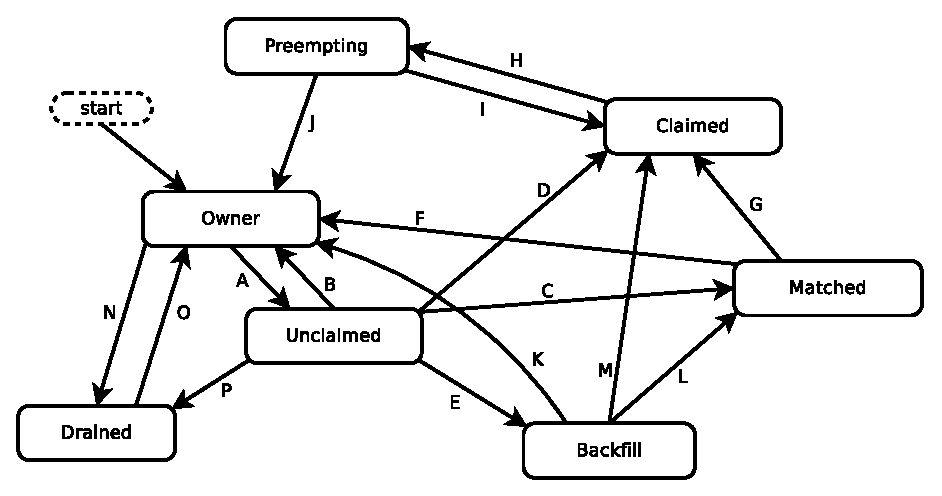
\includegraphics{admin-man/states.eps}
\caption{\label{fig:machine-states}Machine States}
\end{figure}

Each transition is labeled with a letter.
The cause of each transition is described below.


\begin{itemize}


\item Transitions out of the Owner state

\begin{description}

\item[A] The machine switches from Owner to Unclaimed whenever the
  \MacroNI{START} expression no longer locally evaluates to FALSE.
  This indicates that the machine is potentially available to run a
  Condor job.

\end{description}


\item Transitions out of the Unclaimed state

\begin{description}

\item[B] The machine switches from Unclaimed back to Owner whenever the
  \MacroNI{START} expression locally evaluates to FALSE.
  This indicates that the machine is unavailable to run a Condor job
  and is in use by the resource owner.

\item[C] The transition from Unclaimed to Matched happens whenever the
  \Condor{negotiator} matches this resource with a Condor job.

\item[D] The transition from Unclaimed directly to Claimed also happens
  if the \Condor{negotiator} matches this resource with a Condor job.
  In this case the \Condor{schedd} receives the match and initiates
  the claiming protocol with the machine before the \Condor{startd}
  receives the match notification from the \Condor{negotiator}.

\item[E] The transition from Unclaimed to Backfill happens if the
  machine is configured to run backfill computations (see
  section~\ref{sec:Backfill}) and the \MacroNI{START\_BACKFILL}
  expression evaluates to TRUE.

\end{description}


\item Transitions out of the Matched state

\begin{description}

\item[F] The machine moves from Matched to Owner if either the
  \MacroNI{START} expression locally evaluates to FALSE, or if the 
  \Macro{MATCH\_TIMEOUT} timer expires.
  This timeout is used to ensure that if a machine is matched with a
  given \Condor{schedd}, but that \Condor{schedd} does not contact the
  \Condor{startd} to claim it, that the machine will give up on the
  match and become available to be matched again.
  In this case, since the \MacroNI{START} expression does not locally
  evaluate to FALSE, as soon as transition \Bold{F} is complete, the
  machine will immediately enter the Unclaimed state again (via
  transition \Bold{A}).
  The machine might also go from Matched to Owner if the
  \Condor{schedd} attempts to perform the claiming protocol but
  encounters some sort of error.
  Finally, the machine will move into the Owner state if the
  \Condor{startd} receives a \Condor{vacate} command while it is in
  the Matched state.

\item[G] The transition from Matched to Claimed occurs when the
  \Condor{schedd} successfully completes the claiming protocol with
  the \Condor{startd}.

\end{description}

\item Transitions out of the Claimed state

\begin{description}

\item[H] From the Claimed state, the only possible destination is the
  Preempting state.
  This transition can be caused by many reasons:
  \begin{itemize}
  \item The \Condor{schedd} that has claimed the machine has no more
    work to perform and releases the claim
  \item The \MacroNI{PREEMPT} expression evaluates to TRUE (which usually
    means the resource owner has started using the machine again and
    is now using the keyboard, mouse, CPU, etc)  
  \item The \Condor{startd} receives a \Condor{vacate} command
  \item The \Condor{startd} is told to shutdown (either via a signal
    or a \Condor{off} command)
  \item The resource is matched to a job with a better priority
    (either a better user priority, or one where the machine rank is
    higher)
  \end{itemize}

\end{description}


\item Transitions out of the Preempting state

\begin{description}

\item[I] The resource will move from Preempting back to Claimed if the
  resource was matched to a job with a better priority.

\item[J] The resource will move from Preempting to Owner if the
  \MacroNI{PREEMPT} expression had evaluated to TRUE, if \Condor{vacate}
  was used, or if the \MacroNI{START} expression locally evaluates to
  FALSE when the \Condor{startd} has finished evicting whatever job it
  was running when it entered the Preempting state.

\end{description}


\item Transitions out of the Backfill state

\begin{description}

\item[K] The resource will move from Backfill to Owner for the
  following reasons:
  \begin{itemize}
  \item The \MacroNI{EVICT\_BACKFILL} expression evaluates to TRUE
  \item The \Condor{startd} receives a \Condor{vacate} command
  \item The \Condor{startd} is being shutdown
  \end{itemize}
 
\item[L] The transition from Backfill to Matched occurs whenever a
  resource running a backfill computation is matched with a
  \Condor{schedd} that wants to run a Condor job.

\item[M] The transition from Backfill directly to Claimed is similar
  to the transition from Unclaimed directly to Claimed.
  It only occurs if the \Condor{schedd} completes the claiming
  protocol before the \Condor{startd} receives the match notification
  from the \Condor{negotiator}.

\end{description}


\end{itemize}

%%%%%%%%%%%%%%%%%%%%%%%%%%%%%%%%%%%%%%%%%%%%%%%%%%%%%%%%%%%%%%%%%%%%%%
\subsubsection{\label{sec:ClaimedState} The Claimed State and Leases}
%%%%%%%%%%%%%%%%%%%%%%%%%%%%%%%%%%%%%%%%%%%%%%%%%%%%%%%%%%%%%%%%%%%%%%
\index{machine state!claimed, the claim lease}
\index{claim lease}

When a \Condor{schedd} claims a \Condor{startd}, there is a claim lease.
So long as the keep alive updates from the \Condor{schedd} to the
\Condor{startd} continue to arrive, the lease is reset.
If the lease duration passes with no updates,
the \Condor{startd} drops the claim and evicts any jobs the
\Condor{schedd} sent over.

The alive interval is the amount of time between,
or the frequency at which the \Condor{schedd} sends keep alive updates 
to all \Condor{schedd} daemons.
An alive update resets the claim lease at the \Condor{startd}.
Updates are UDP packets.

Initially, as when the \Condor{schedd} starts up,
the alive interval starts at the value set by the 
configuration variable \Macro{ALIVE\_INTERVAL}.  
It may be modified when a job is started.
The job's ClassAd attribute \Attr{JobLeaseDuration} is checked.
If the value of \Expr{JobLeaseDuration/3} is less than the current
alive interval,
then the alive interval is set to either this lower value
or the imposed lowest limit on the alive interval of 10 seconds.
Thus, the alive interval starts at \MacroNI{ALIVE\_INTERVAL} and goes down,
never up.

If a claim lease expires,
the \Condor{startd} will drop the claim.
The length of the claim lease is 
the job's ClassAd attribute \Attr{JobLeaseDuration}.
\Attr{JobLeaseDuration} defaults to 20 minutes time,
except when explicitly
set within the job's submit description file.
If \Attr{JobLeaseDuration} is explicitly set to 0, 
or it is not set as may be the case for a Web Services job
that does not define the attribute, 
then \Attr{JobLeaseDuration} is given the Undefined value.
Further, when undefined,
the claim lease duration is calculated with
\Expr{MAX\_CLAIM\_ALIVES\_MISSED * alive interval}.
The alive interval is the \emph{current} value,
as sent by the \Condor{schedd}.
If the \Condor{schedd} reduces the current alive interval,
it does not update the \Condor{startd}.

%%%%%%%%%%%%%%%%%%%%%%%%%%%%%%%%%%%%%%%%%%%%%%%%%%%%%%%%%%%%%%%%%%%%%%
\subsection{\label{sec:Activities}
Machine Activities}
%%%%%%%%%%%%%%%%%%%%%%%%%%%%%%%%%%%%%%%%%%%%%%%%%%%%%%%%%%%%%%%%%%%%%%

\index{machine activity}
\index{activity!of a machine}
Within some machine states,
\Term{activities} of the machine are defined.
The state has meaning regardless of activity.
Differences between activities are significant.
Therefore, a ``state/activity'' pair describes
a machine.
The following list describes all the possible state/activity pairs.

\begin{itemize}

\item Owner
\begin{description}
\index{machine activity!Idle}
\item[Idle] This is the only activity for Owner state.  As far as
  Condor is concerned the machine is Idle, since it is not doing
  anything for Condor.
\end{description}

\index{machine activity!Unclaimed}
\item Unclaimed
\begin{description}
  \item[Idle] This is the normal activity of Unclaimed machines.
    The machine is still Idle in that the machine owner is willing to
    let Condor jobs run, but Condor is not using the
    machine for anything.
  
  \index{machine activity!Benchmarking}
  \item[Benchmarking] The machine is running benchmarks to
    determine the speed on this machine.
    This activity only occurs in the Unclaimed state.
    How often the activity occurs is
    determined by the \MacroNI{RUNBENCHMARKS} expression.
\end{description}

\item Matched
\begin{description}
  \item[Idle] When Matched, the machine is still Idle to Condor.
\end{description}

\item Claimed
\begin{description}
\item[Idle] In this activity, the machine has been claimed, but the
  schedd that claimed it has yet to \Term{activate} the claim by
  requesting a \Condor{starter} to be spawned to service a job.
  The machine returns to this state (usually briefly) when jobs
  (and therefore \Condor{starter}) finish.
  
\index{machine activity!Busy}
\item[Busy] Once a \Condor{starter} has been started and the claim is
  active, the machine moves to the Busy activity to signify that it is
  doing something as far as Condor is concerned.
  
\index{machine activity!Suspended}
\item[Suspended] If the job is suspended by Condor, the machine goes
  into the Suspended activity.
  The match between the schedd and machine has not been broken (the
  claim is still valid), but the job is not making any progress and
  Condor is no longer generating a load on the machine.

\index{machine activity!Retiring}
\item[Retiring] When an active claim is about to be preempted for any
reason, it enters retirement, while it waits for the current job to
finish.  The \MacroNI{MaxJobRetirementTime} expression determines how
long to wait (counting since the time the job started).  Once the job
finishes or the retirement time expires, the Preempting state is
entered.
\end{description}

\item Preempting
  The preempting state is used for evicting a Condor job from a given
  machine.
  When the machine enters the Preempting state, it checks the
  \MacroNI{WANT\_VACATE} expression to determine its activity.

\begin{description}
\index{machine activity!Vacating}
\item[Vacating] In the Vacating activity, the job that was running is
  in the process of checkpointing.
  As soon as the checkpoint process completes,
  the machine moves into either the Owner state or the
  Claimed state, depending on the reason for its preemption.
  
\index{machine activity!Killing}
\item[Killing] Killing means that the machine has requested the running
  job to exit the machine immediately, without checkpointing.
\end{description}

\index{machine activity!Backfill}
\item Backfill
\begin{description}
\item[Idle] The machine is configured to run backfill jobs and is
  ready to do so, but it has not yet had a chance to spawn a backfill
  manager (for example, the BOINC client).

\item[Busy] The machine is performing a backfill computation.

\item[Killing] The machine was running a backfill computation, but it
  is now killing the job to either return resources to the machine
  owner, or to make room for a regular Condor job.

\end{description}

\index{machine activity!Drained}
\item Drained
\begin{description}

\item[Idle] All slots have been drained.

\item[Retiring] This slot has been drained.  It is waiting for other
  slots to finish draining.

\end{description}

\end{itemize}

Figure~\ref{fig:machine-activities} on
page~\pageref{fig:machine-activities} gives the overall view of all
machine states and activities and shows the possible transitions
from one to another within the Condor system.  
Each transition is labeled with a number on the diagram, and
transition numbers referred to in this manual will be \Bold{bold}.  

\index{machine state and activities figure}
\index{state and activities figure}
\index{activities and state figure}
\begin{figure}[hbt]
\centering
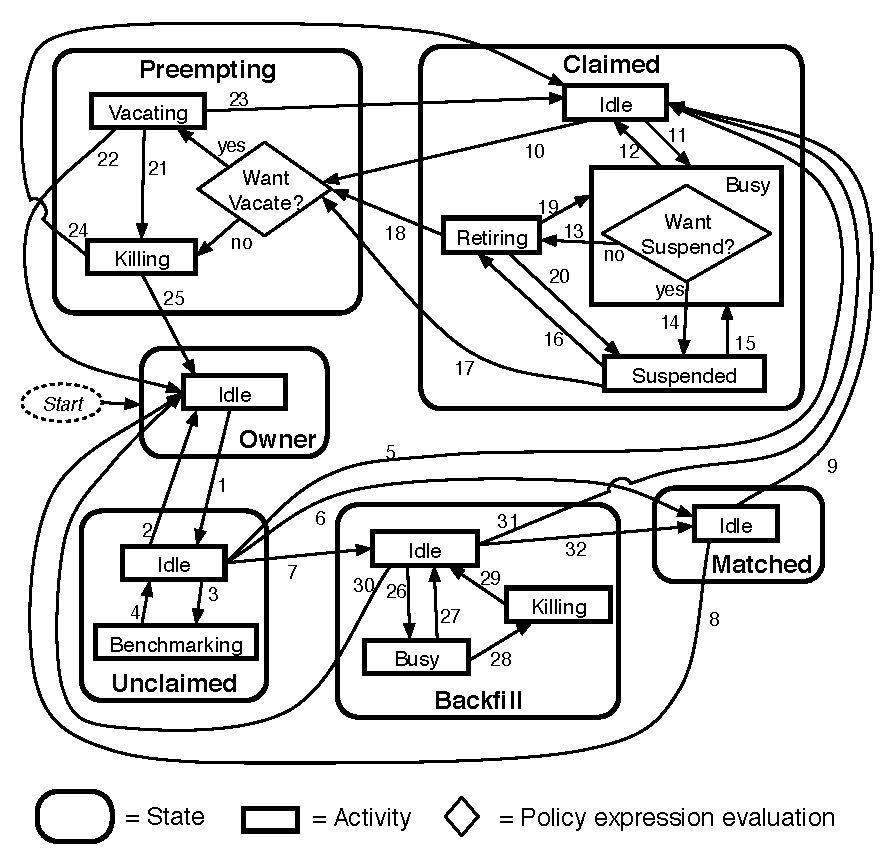
\includegraphics{admin-man/machine-activities.eps}
\caption{\label{fig:machine-activities}Machine States and Activities}
\end{figure}

Various expressions are used to determine when and if many of these
state and activity transitions occur.  Other transitions are initiated
by parts of the Condor protocol (such as when the \Condor{negotiator}
matches a machine with a schedd).  The following section describes the
conditions that lead to the various state and activity transitions.

%%%%%%%%%%%%%%%%%%%%%%%%%%%%%%%%%%%%%%%%%%%%%%%%%%%%%%%%%%%%%%%%%%%%%%
\subsection{\label{sec:State-and-Activity-Transitions}
State and Activity Transitions}
%%%%%%%%%%%%%%%%%%%%%%%%%%%%%%%%%%%%%%%%%%%%%%%%%%%%%%%%%%%%%%%%%%%%%%

\index{machine state!transitions|(}
\index{machine activity!transitions|(}
\index{state!transitions|(}
\index{activity!transitions|(}
This section traces through all possible state and activity
transitions within a machine and describes the conditions under which
each one occurs.
Whenever a transition occurs, Condor records when the machine entered its
new activity and/or new state.
These times are often used to write expressions that determine
when further transitions occurred.
For example, enter the Killing activity if a machine has been in
the Vacating activity longer than a specified amount of time. 

%%%%%%%%%%%%%%%%%%%%%%%%%%%%%%%%%%%%%%%%%%%%%%%%%%%%%%%%%%%%%%%%%%%%%%
\subsubsection{\label{sec:Owner-State}
Owner State}
%%%%%%%%%%%%%%%%%%%%%%%%%%%%%%%%%%%%%%%%%%%%%%%%%%%%%%%%%%%%%%%%%%%%%%

\index{machine state!Owner}
\index{owner state}
When the startd is first spawned, the machine it represents enters the
Owner state. 
The machine remains in the Owner state while the
expression \Macro{IS\_OWNER} is TRUE.
If the \MacroNI{IS\_OWNER} expression is FALSE,
then the machine transitions to the Unclaimed state.
The default value for the 
\MacroNI{IS\_OWNER} expression is optimized for a shared resource
\begin{verbatim}
START =?= FALSE
\end{verbatim}
So,
the machine will remain in the Owner state as long as the \MacroNI{START}
expression locally evaluates to FALSE.
Section~\ref{sec:Start-Expr} provides more detail on the
\MacroNI{START} expression.
If the \MacroNI{START} locally evaluates to TRUE or cannot be locally
evaluated (it evaluates to UNDEFINED), transition \Bold{1}
occurs and the machine enters the Unclaimed state.
The \MacroNI{IS\_OWNER} expression is locally evaluated by the machine,
and should not reference job ClassAd attributes, which would be
UNDEFINED.

For dedicated resources, the recommended value for the \MacroNI{IS\_OWNER}
expression is FALSE.

The Owner state represents a resource that is in use by its
interactive owner (for example, if the keyboard is being used).
The Unclaimed state represents a resource that is neither in use by
its interactive user, nor the Condor system.
From Condor's point of view, there is little difference between the
Owner and Unclaimed states.
In both cases, the resource is not currently in use by the Condor
system.
However, if a job matches the resource's \MacroNI{START} expression, the
resource is available to run a job, regardless of if it is in the
Owner or Unclaimed state.
The only differences between the two states are how the resource shows
up in \Condor{status} and other reporting tools, and the fact that
Condor will not run benchmarking on a resource in the Owner state.
As long as the \MacroNI{IS\_OWNER} expression is TRUE, the machine is
in the Owner State.
When the \MacroNI{IS\_OWNER} expression is FALSE, the machine goes into
the Unclaimed State.

Here is an example that assumes that an \MacroNI{IS\_OWNER}
expression is not present in the configuration.
If the \MacroNI{START} expression is
\begin{verbatim}
START = KeyboardIdle > 15 * $(MINUTE) && Owner == "coltrane" 
\end{verbatim}
and if \Attr{KeyboardIdle} is 34 seconds,
then the machine would remain in the Owner state.
Owner is undefined, and
\verb@anything && FALSE@ is FALSE.

If, however, the \MacroNI{START} expression is
\begin{verbatim}
        START = KeyboardIdle > 15 * $(MINUTE) || Owner == "coltrane"
\end{verbatim}
and \Attr{KeyboardIdle} is 34 seconds, then the machine
leaves the Owner state and becomes Unclaimed.
This is because
\verb@FALSE || UNDEFINED@ is UNDEFINED.
So, while this machine is not available to just anybody,
if user coltrane has jobs submitted, the machine is willing to run them.
Any other user's jobs have to wait
until \Attr{KeyboardIdle} exceeds 15 minutes.
However, since coltrane might claim this resource,
but has not yet, the machine goes to the Unclaimed state.

While in the Owner state, the startd polls the status of the
machine every \Macro{UPDATE\_INTERVAL} to see if anything has changed
that would lead it to a different state.
This minimizes the impact on the Owner
while the Owner is using the machine.
Frequently waking up, computing load averages, checking the access
times on files, computing free swap space take time,
and there is nothing
time critical that the startd needs to be sure to notice as soon as it
happens.
If the \MacroNI{START} expression evaluates to TRUE and five
minutes pass before the startd notices,
that's a drop in the bucket of high-throughput computing.

The machine can only transition to the Unclaimed state from the Owner
state. It does so when the \MacroNI{IS\_OWNER} expression no longer
evaluates to FALSE.  By default, that happens when \MacroNI{START} no longer
locally evaluates to FALSE.

Whenever the machine is not actively running a job, it will transition
back to the Owner state if \MacroNI{IS\_OWNER} evaluates to TRUE.  Once a
job is started, the value of \MacroNI{IS\_OWNER} does not matter; the job
either runs to completion or is preempted.  Therefore, you must
configure the preemption policy if you want to transition back to the
Owner state from Claimed Busy.

%%%%%%%%%%%%%%%%%%%%%%%%%%%%%%%%%%%%%%%%%%%%%%%%%%%%%%%%%%%%%%%%%%%%%%
\subsubsection{\label{sec:Unclaimed-State}Unclaimed State}
%%%%%%%%%%%%%%%%%%%%%%%%%%%%%%%%%%%%%%%%%%%%%%%%%%%%%%%%%%%%%%%%%%%%%%
\index{machine state!Unclaimed}
\index{unclaimed state}

If the \MacroNI{IS\_OWNER} expression becomes TRUE, then the machine returns
to the Owner state.
If the \MacroNI{IS\_OWNER} expression becomes FALSE, then the machine remains
in the Unclaimed state.
If the \MacroNI{IS\_OWNER} expression is not present in the configuration files,
then the default value for the \MacroNI{IS\_OWNER} expression is 
\begin{verbatim}
START =?= FALSE
\end{verbatim}
so that
while in the Unclaimed state, if the \MacroNI{START} expression locally
evaluates to FALSE, the machine returns to the Owner state by
transition \Bold{2}.

When in the Unclaimed state,
the \Macro{RUNBENCHMARKS}
expression is relevant.
If \MacroNI{RUNBENCHMARKS} evaluates to TRUE while the machine
is in the Unclaimed state,
then the machine will transition from the Idle
activity to the Benchmarking activity (transition \Bold{3}) and
perform benchmarks to determine \Attr{MIPS} and \Attr{KFLOPS}.  
When the benchmarks complete, the machine returns to the Idle activity
(transition \Bold{4}).

The startd automatically inserts an attribute, \Attr{LastBenchmark},
whenever it runs benchmarks, so commonly \Attr{RunBenchmarks} is
defined in terms of this attribute, for example:
\begin{verbatim}
        BenchmarkTimer = (CurrentTime - LastBenchmark)
        RunBenchmarks = $(BenchmarkTimer) >= (4 * $(HOUR))
\end{verbatim}
Here, a macro, \MacroNI{BenchmarkTimer} is defined to help write the
expression.
This macro holds the time since the last benchmark,
so when this time exceeds 4 hours, we run the benchmarks again.
The startd keeps a weighted average of these benchmarking
results to try to get the most accurate numbers possible.
This is why
it is desirable for 
the startd to run them more than once in its lifetime.

\Note \Attr{LastBenchmark} is initialized to 0 before benchmarks
have ever been run.
To have the \Condor{startd} run benchmarks as soon as the machine is
Unclaimed (if it has not done so already),
include a term using \Attr{LastBenchmark} as in the example above.

\Note If \MacroNI{RUNBENCHMARKS} is defined and set to something
other than FALSE, the startd will automatically run one set of
benchmarks when it first starts up.
To disable benchmarks, both at startup and at any time thereafter,
set \MacroNI{RUNBENCHMARKS} to FALSE or comment it out of the
configuration file.

From the Unclaimed state, the machine can go to four other possible
states: Owner (transition \Bold{2}), Backfill/Idle, Matched, or
Claimed/Idle.

Once the \Condor{negotiator} matches an Unclaimed machine with a
requester at a given schedd, the negotiator sends a command to both
parties, notifying them of the match.  
If the schedd receives that notification and initiates the claiming
procedure with the machine before the negotiator's message gets to the
machine, the Match state is skipped,
and the machine goes
directly to the Claimed/Idle state (transition \Bold{5}).
However, normally the machine will enter the Matched state (transition
\Bold{6}), even if it is only for a brief period of time.

If the machine has been configured to perform backfill jobs (see
section~\ref{sec:Backfill}), while it is in Unclaimed/Idle it will
evaluate the \Macro{START\_BACKFILL} expression.
Once \MacroNI{START\_BACKFILL} evaluates to TRUE, the machine will enter
the Backfill/Idle state (transition \Bold{7}) to begin the process of
running backfill jobs.


%%%%%%%%%%%%%%%%%%%%%%%%%%%%%%%%%%%%%%%%%%%%%%%%%%%%%%%%%%%%%%%%%%%%%%
\subsubsection{\label{sec:Matched-State}Matched State}
%%%%%%%%%%%%%%%%%%%%%%%%%%%%%%%%%%%%%%%%%%%%%%%%%%%%%%%%%%%%%%%%%%%%%%
\index{machine state!Matched}
\index{matched state}

The Matched state is not very interesting to Condor.
Noteworthy in this state is that the machine lies about its \MacroNI{START}
expression while in this state and says that \Expr{Requirements} are
\Expr{False} to prevent being matched again before it has been claimed.
Also interesting is that
the startd starts a timer to make sure it does not stay in the
Matched state too long.
The timer is set with the \Macro{MATCH\_TIMEOUT}
\label{param:MatchTimeout} configuration file macro.
It is specified in seconds and defaults to 120 (2 minutes).
If the schedd that was matched with this machine does not
claim it within this period of time, the machine gives up,
and goes back into the Owner state via transition \Bold{8}.
It will probably leave the Owner state right away for the
Unclaimed state again and wait for another match. 

At any time while the machine is in the Matched state, if the
\MacroNI{START} expression locally evaluates to FALSE, the machine enters
the Owner state directly (transition \Bold{8}).

If the schedd that was matched with the machine claims it before the
\MacroNI{MATCH\_TIMEOUT} expires, the machine goes into the Claimed/Idle
state (transition \Bold{9}).

%%%%%%%%%%%%%%%%%%%%%%%%%%%%%%%%%%%%%%%%%%%%%%%%%%%%%%%%%%%%%%%%%%%%%%
\subsubsection{\label{sec:Claimed-State}Claimed State}
%%%%%%%%%%%%%%%%%%%%%%%%%%%%%%%%%%%%%%%%%%%%%%%%%%%%%%%%%%%%%%%%%%%%%%
\index{machine state!Claimed}
\index{claimed state}

The Claimed state is certainly the most complex state.
It has the most possible activities and the most expressions that
determine its next activities.
In addition, the \Condor{checkpoint} and \Condor{vacate} commands affect
the machine when it is in the Claimed state.
In general, there are two sets of expressions that might take effect.
They depend on the universe of the request: standard or vanilla.
The standard universe expressions are the normal expressions.
For example:
\begin{verbatim}
        WANT_SUSPEND            = True
        WANT_VACATE             = $(ActivationTimer) > 10 * $(MINUTE)
        SUSPEND                 = $(KeyboardBusy) || $(CPUBusy)
        ...
\end{verbatim}

The vanilla expressions have the string``\_VANILLA'' appended to their names.
For example:
\begin{verbatim}
        WANT_SUSPEND_VANILLA    = True
        WANT_VACATE_VANILLA     = True
        SUSPEND_VANILLA         = $(KeyboardBusy) || $(CPUBusy)
        ...
\end{verbatim}

Without specific vanilla versions, the normal versions
will be used for all jobs, including vanilla jobs.  
In this manual, the normal expressions are referenced.
The difference exists for the
the resource owner that might want the machine
to behave differently for vanilla jobs, since they cannot checkpoint.
For example, owners may want vanilla jobs to remain suspended for
longer than standard jobs.

While Claimed, the \Macro{POLLING\_INTERVAL} takes effect, and the
startd polls the machine much more frequently to evaluate its
state.

If the machine owner starts typing on the console again,
it is best to notice this as
soon as possible to be able to start doing whatever 
the machine owner wants at that point.
For SMP machines, if any slot is in the Claimed state, the
startd polls the machine frequently.
If already polling one slot, it does not
cost much to evaluate the state of all the slots at
the same time.

There are a variety of events that may cause the startd to try to get
rid of or temporarily suspend a running job.  Activity on the
machine's console, load from other jobs, or shutdown of the startd via
an administrative command are all possible sources of interference.
Another one is the appearance of a higher priority claim to the
machine by a different Condor user.

Depending on the configuration, the startd may respond quite
differently to activity on the machine, such as keyboard activity or
demand for the cpu from processes that are not managed by Condor.  The
startd can be configured to completely ignore such activity or to
suspend the job or even to kill it.  A standard configuration for a desktop
machine might be to go through
successive levels of getting the job out of the way.
The first and least costly to the job is suspending it.
This works for both standard and vanilla jobs.
If suspending the job for a short while does not satisfy the machine
owner (the owner is still using the machine after a specific period of
time), the startd moves on to vacating the job.
Vacating a standard universe job
involves performing a checkpoint so that the work already completed
is not lost.  Vanilla jobs are sent a \Term{soft kill signal} so that they
can gracefully shut down if necessary; the default is \verb@SIGTERM@.
If vacating does not satisfy the machine owner (usually because it is
taking too long and the owner wants their machine back \emph{now}),
the final, most drastic stage is reached: killing.  
Killing is a quick death to the job, using a hard-kill signal that cannot
be intercepted by the application.  For vanilla jobs that do no special
signal handling, vacating and killing are equivalent.

The \MacroNI{WANT\_SUSPEND} expression determines if the machine will
evaluate the \MacroNI{SUSPEND} expression to consider entering the
Suspended activity.
The \MacroNI{WANT\_VACATE} expression determines what happens when the
machine enters the Preempting state.
It will go to the Vacating
activity or directly to Killing. 
If one or both of these expressions evaluates to FALSE, the machine
will skip that stage of getting rid of the job and proceed directly to
the more drastic stages.

When the machine first enters the Claimed state, it goes to the Idle
activity.  From there, it has two options.  
It can enter the Preempting state via transition \Bold{10} (if a 
\Condor{vacate} arrives, or if the \MacroNI{START} expression locally
evaluates to FALSE),  
or it can enter the Busy activity (transition \Bold{11}) if the
schedd that has claimed the machine decides to activate the claim and
start a job.

From Claimed/Busy, the machine can transition to three other state/activity
pairs.
The startd evaluates the \MacroNI{WANT\_SUSPEND} expression to decide
which other expressions to evaluate.  
If \MacroNI{WANT\_SUSPEND} is TRUE, then the startd evaluates the
\MacroNI{SUSPEND} expression.
If \MacroNI{WANT\_SUSPEND} is any value other than TRUE, then the startd will
evaluate the \MacroNI{PREEMPT} expression and skip the Suspended activity
entirely.
By transition, the possible state/activity destinations from Claimed/Busy:

\begin{description}
  
\item[Claimed/Idle] If the starter that is serving a given job exits
  (for example because the jobs completes), the machine will go
  to Claimed/Idle (transition \Bold{12}).
  
\item[Claimed/Retiring] If \MacroNI{WANT\_SUSPEND} is FALSE and the
  \MacroNI{PREEMPT} expression is TRUE, the machine enters the
  Retiring activity (transition \Bold{13}).  From there, it
  waits for a configurable amount of time for the job to finish
  before moving on to preemption.

  Another reason the machine would go from Claimed/Busy to
  Claimed/Retiring is if the \Condor{negotiator} matched the machine
  with a ``better'' match.  This better match could either be from the
  machine's perspective using the startd \MacroNI{RANK} expression,
  or it could be from the negotiator's perspective due to
  a job with a higher user priority.

  Another case resulting in a transition to Claimed/Retiring is when
  the startd is being shut down.  The only exception is a ``fast''
  shutdown, which bypasses retirement completely.
  
\item[Claimed/Suspended] If both the \MacroNI{WANT\_SUSPEND} and
  \MacroNI{SUSPEND} expressions evaluate to TRUE, the machine
  suspends the job (transition \Bold{14}).
  
\end{description}
  
If a \Condor{checkpoint} command arrives,
or the \MacroNI{PERIODIC\_CHECKPOINT} expression evaluates to TRUE,
there is no state change.
The startd has no way of knowing when this process completes,
so periodic checkpointing can not be another state.
Periodic checkpointing remains in the Claimed/Busy state
and appears as a running job.

From the Claimed/Suspended state, the following transitions
may occur:

\begin{description}
  
\item[Claimed/Busy] If the \MacroNI{CONTINUE} expression evaluates to
  TRUE, the machine resumes the job and enters the
  Claimed/Busy state (transition \Bold{15}) or the Claimed/Retiring
  state (transition \Bold{16}), depending on whether the claim
  has been preempted.

\item[Claimed/Retiring] If the \MacroNI{PREEMPT} expression is TRUE, the machine
  will enter the Claimed/Retiring activity (transition \Bold{16}).

\item[Preempting] If the claim is in suspended retirement and the
  retirement time expires, the job enters the Preempting state
  (transition \Bold{17}).  This is only possible if
  \MacroNI{MaxJobRetirementTime} \emph{decreases} during the suspension.


\end{description}

For the Claimed/Retiring state, the following transitions may occur:

\begin{description}

\item[Preempting] If the job finishes or the job's run time exceeds
the value defined for the job ClassAd attribute \Attr{MaxJobRetirementTime},
the Preempting state is entered
(transition \Bold{18}).  The run time is computed from the time when the
job was started by the startd minus any suspension time.  When retiring
due to \Condor{startd} daemon shutdown or restart,
it is possible for the administrator to issue a
\Term{peaceful} shutdown command, which causes \MacroNI{MaxJobRetirementTime}
to effectively be infinite, avoiding any killing of jobs.  It is also
possible for the administrator to issue a \Term{fast} shutdown command,
which causes
\MacroNI{MaxJobRetirementTime} to be effectively 0.

\item[Claimed/Busy] If the startd was retiring because of a preempting
claim only and the preempting claim goes away, the normal Claimed/Busy
state is resumed (transition \Bold{19}).  If instead the retirement
is due to owner activity (\MacroNI{PREEMPT}) or the startd is being shut down,
no unretirement is possible.

\item[Claimed/Suspended] In exactly the same way that suspension may
happen from the Claimed/Busy state, it may also happen during the
Claimed/Retiring state (transition \Bold{20}).
In this case, when the job continues from suspension, it moves back
into Claimed/Retiring (transition \Bold{16}) instead of Claimed/Busy
(transition \Bold{15}).

\end{description}


%%%%%%%%%%%%%%%%%%%%%%%%%%%%%%%%%%%%%%%%%%%%%%%%%%%%%%%%%%%%%%%%%%%%%%
\subsubsection{\label{sec:Preempting-State}Preempting State}
%%%%%%%%%%%%%%%%%%%%%%%%%%%%%%%%%%%%%%%%%%%%%%%%%%%%%%%%%%%%%%%%%%%%%%
\index{machine state!Preempting}
\index{preempting state}

The Preempting state is less complex than the Claimed state.
There are two activities.
Depending on the value of \MacroNI{WANT\_VACATE}, a machine will
be in the
Vacating activity (if TRUE) or the Killing activity (if FALSE).  

While in the Preempting state (regardless of activity) the machine
advertises its \Expr{Requirements} expression as FALSE to signify that
it is not available for further matches, either because it is about to
transition
to the Owner state, or because it has already been matched with
one preempting match, and further preempting matches are disallowed
until the machine has been claimed by the new match.

The main function of the Preempting state is to get rid of the starter
associated with the resource.  If the \Condor{starter} associated with
a given claim exits while the machine is still in the Vacating
activity, then the job successfully completed a graceful shutdown.
For standard universe jobs, this means that a checkpoint was saved.
For other jobs, this means the application was given an opportunity to
do a graceful shutdown, by intercepting the soft kill signal.

If the machine is in the Vacating activity, it keeps evaluating the 
\MacroNI{KILL} expression.
As soon as this expression evaluates to TRUE,
the machine enters the Killing activity (transition \Bold{21}).
If the Vacating activity lasts for as long as the maximum
vacating time, then the machine also enters the Killing activity.
The maximum vacating time is determined by the configuration variable
\Macro{MachineMaxVacateTime}.
This may be adjusted by the setting of the job ClassAd
attribute \Attr{JobMaxVacateTime}.

When the starter exits, or if there was no starter running when the
machine enters the Preempting state (transition \Bold{10}),
the other purpose of the Preempting state is completed:
notifying the schedd that had claimed this machine that the claim is
broken.

At this point, the machine enters either the Owner state by
transition \Bold{22} (if the job was preempted because the machine
owner came back) or the Claimed/Idle state by transition \Bold{23}
(if the job was preempted because a better match was found).

If the machine enters the Killing activity, (because either
\MacroNI{WANT\_VACATE} was FALSE or the \MacroNI{KILL} expression evaluated
to TRUE), it attempts to force the \Condor{starter} to immediately
kill the underlying Condor job.
Once the machine has begun to hard kill the Condor job, the
\Condor{startd} starts a timer, the length of which is defined by the
\Macro{KILLING\_TIMEOUT} \label{param:KillingTimeout} macro.
This macro is defined in seconds and defaults to 30.
If this timer expires and the machine is still in
the Killing activity, something has gone seriously wrong with the
\Condor{starter} and the startd tries to vacate the job immediately by
sending SIGKILL to all of the \Condor{starter}'s children, and then to
the \Condor{starter} itself.

Once the \Condor{starter} has killed off all the processes associated
with the job and exited, and once the schedd that had claimed the
machine is notified that the claim is broken, the machine will leave
the Preempting/Killing state.
If the job was preempted because a better match was found, the machine
will enter Claimed/Idle (transition \Bold{24}).
If the preemption was caused by the machine owner (the \MacroNI{PREEMPT}
expression evaluated to TRUE, \Condor{vacate} was used, etc), the
machine will enter the Owner state (transition \Bold{25}).


%%%%%%%%%%%%%%%%%%%%%%%%%%%%%%%%%%%%%%%%%%%%%%%%%%%%%%%%%%%%%%%%%%%%%%
\subsubsection{\label{sec:Backfill-State}Backfill State}
%%%%%%%%%%%%%%%%%%%%%%%%%%%%%%%%%%%%%%%%%%%%%%%%%%%%%%%%%%%%%%%%%%%%%%
\index{machine state!Backfill}
\index{backfill state}

The Backfill state is used whenever the machine is performing low
priority background tasks to keep itself busy.
For more information about backfill support in Condor, see
section~\ref{sec:Backfill} on page~\pageref{sec:Backfill}.
This state is only used if the machine has been configured to enable
backfill computation, if a specific backfill manager has been
installed and configured, and if the machine is otherwise idle (not
being used interactively or for regular Condor computations).
If the machine meets all these requirements, and the
\MacroNI{START\_BACKFILL} expression evaluates to TRUE, the machine will
move from the Unclaimed/Idle state to Backfill/Idle (transition
\Bold{7}).

Once a machine is in Backfill/Idle, it will immediately attempt to
spawn whatever backfill manager it has been configured to use
(currently, only the BOINC client is supported as a backfill manager
in Condor).
Once the BOINC client is running, the machine will enter
Backfill/Busy (transition \Bold{26}) to indicate that it is now
performing a backfill computation.

\Note On SMP machines, the \Condor{startd} will only spawn a single
instance of the BOINC client, even if multiple slots are
available to run backfill jobs.
Therefore, only the first machine to enter Backfill/Idle will cause a
copy of the BOINC client to start running.
If a given slot on an SMP enters the Backfill state and a
BOINC client is already running under this \Condor{startd}, the
slot will immediately enter Backfill/Busy without waiting
to spawn another copy of the BOINC client.

If the BOINC client ever exits on its own (which normally wouldn't
happen), the machine will go back to Backfill/Idle (transition
\Bold{27}) where it will immediately attempt to respawn the BOINC
client (and return to Backfill/Busy via transition \Bold{26}).

As the BOINC client is running a backfill computation, a number of
events can occur that will drive the machine out of the Backfill
state.
The machine can get matched or claimed for a Condor job, interactive
users can start using the machine again, the machine might be evicted
with \Condor{vacate}, or the \Condor{startd} might be shutdown.
All of these events cause the \Condor{startd} to kill the BOINC client
and all its descendants, and enter the Backfill/Killing state
(transition \Bold{28}).

Once the BOINC client and all its children have exited the system, the
machine will enter the Backfill/Idle state to indicate that the BOINC
client is now gone (transition \Bold{29}).
As soon as it enters Backfill/Idle after the BOINC client exits, the
machine will go into another state, depending on what caused the BOINC
client to be killed in the first place.

If the \MacroNI{EVICT\_BACKFILL} expression evaluates to TRUE while a
machine is in Backfill/Busy, after the BOINC client is gone, the
machine will go back into the Owner/Idle state (transition
\Bold{30}).
The machine will also return to the Owner/Idle state after the BOINC
client exits if \Condor{vacate} was used, or if the \Condor{startd} is
being shutdown.

When a machine running backfill jobs is matched with a requester that
wants to run a Condor job, the machine will either enter the Matched
state, or go directly into Claimed/Idle.
As with the case of a machine in Unclaimed/Idle (described above), the
\Condor{negotiator} informs both the \Condor{startd} and the
\Condor{schedd} of the match, and the exact state transitions at the
machine depend on what order the various entities initiate
communication with each other.
If the \Condor{schedd} is notified of the match and sends a request to
claim the \Condor{startd} before the \Condor{negotiator} has a chance
to notify the \Condor{startd}, once the BOINC client exits, the
machine will immediately enter Claimed/Idle (transition \Bold{31}).
Normally, the notification from the \Condor{negotiator} will reach the
\Condor{startd} before the \Condor{schedd} attempts to claim it.
In this case, once the BOINC client exits, the machine will enter
Matched/Idle (transition \Bold{32}).


%%%%%%%%%%%%%%%%%%%%%%%%%%%%%%%%%%%%%%%%%%%%%%%%%%%%%%%%%%%%%%%%%%%%%%
\subsection{\label{sec:State-Expression-Summary}
State/Activity Transition Expression Summary}
%%%%%%%%%%%%%%%%%%%%%%%%%%%%%%%%%%%%%%%%%%%%%%%%%%%%%%%%%%%%%%%%%%%%%%
\index{machine state!transitions summary}
\index{machine activity!transitions summary}
\index{state!transitions summary}
\index{activity!transitions summary}
This section is a summary of the information from the
previous sections.
It serves as a quick reference.

\begin{description}
  
\item[\Macro{START}] When TRUE, the machine is willing to spawn
  a remote Condor job.
  
\item[\Macro{RUNBENCHMARKS}] While in the Unclaimed state, the machine
  will run benchmarks whenever TRUE.
  
\item[\Macro{MATCH\_TIMEOUT}] If the machine has been in the Matched
  state longer than this value, it will transition to the Owner state.
  
\item[\Macro{WANT\_SUSPEND}] If TRUE, the machine evaluates
  the \MacroNI{SUSPEND} expression to see if it should transition to the
  Suspended activity.  
  If any value other than TRUE, the machine will look at
  the \MacroNI{PREEMPT} expression.
  
\item[\Macro{SUSPEND}] If \MacroNI{WANT\_SUSPEND} is TRUE, and the machine
  is in the Claimed/Busy state, it enters the Suspended activity
  if \MacroNI{SUSPEND} is TRUE.
  
\item[\Macro{CONTINUE}] If the machine is in the Claimed/Suspended
  state, it enter the Busy activity if \MacroNI{CONTINUE} is TRUE.
  
\item[\Macro{PREEMPT}] If the machine is either in the Claimed/Suspended
  activity, or is in the Claimed/Busy activity and
  \MacroNI{WANT\_SUSPEND} is FALSE, the machine enters the Claimed/Retiring
  state whenever \MacroNI{PREEMPT} is TRUE. 

\item[\Macro{CLAIM\_WORKLIFE}] If provided, this expression specifies
the number of seconds during which a claim will continue accepting new
jobs.  Once this time expires, any existing job may continue to run as
usual, but once it finishes or is preempted, the claim is closed.
This may be useful if you want to force periodic renegotiation of
resources without preemption having to occur.  For example, if you
have some low-priority jobs which should never be interrupted with
kill signals, you could prevent them from being killed with
\Attr{MaxJobRetirementTime}, but now high-priority jobs may have to
wait in line when they match to a machine that is busy running one of
these uninterruptible jobs.  You can prevent the high-priority jobs
from ever matching to such a machine by using a rank expression in the
job or in the negotiator's rank expressions, but then the low-priority
claim will never be interrupted; it can keep running more jobs.  The
solution is to use \MacroNI{CLAIM\_WORKLIFE} to force the claim to stop
running additional jobs after a certain amount of time.
The default value for \MacroNI{CLAIM\_WORKLIFE} is -1, which is treated
as an infinite claim worklife, so claims may be held indefinitely (as
long as they are not preempted and the schedd does not relinquish
them, of course).

\item[\Macro{MachineMaxVacateTime}] When the machine enters the
Preempting/Vacating state, this expression specifies the maximum
time in seconds that the \Condor{startd} will wait for the job to
finish.  The job may adjust the wait time by setting
\AdAttr{JobMaxVacateTime}.  If the job's setting is less than the
machine's, the job's is used.  If the job's setting is larger than
the machine's, the result depends on whether the job has any excess
retirement time.  If the job has more retirement time left than the
machine's maximum vacate time setting, then retirement time will be
converted into vacating time, up to the amount of
\Attr{JobMaxVacateTime}.  Once the vacating time expires, the
job is hard-killed.  The \Macro{KILL} expression may be used
to abort the graceful shutdown of the job at any time.

\item[\Macro{MAXJOBRETIREMENTTIME}] If the machine is in the
Claimed/Retiring state, this expression specifies the maximum time (in
seconds) that the \Condor{startd} will wait for the job to finish.
The clock starts when the
job is started and is paused during any suspension.  The job may
provide its own expression for \Attr{MaxJobRetirementTime}, but this
can only be used to take \emph{less} than the time granted by the
\Condor{startd}, never more.  For convenience, standard universe and
nice\_user jobs are submitted with a default retirement time of 0, so
they will never wait in retirement unless the user overrides the
default.

The machine enters the Preempting state with the goal of finishing
shutting down the job by the end of the retirement time.  If the job
vacating policy grants the job X seconds of vacating time, the
transition to the Preempting state will happen X seconds before the
end of the retirement time, so that the hard-killing of the job will not
happen until the end of the retirement time, if the job does not finish
shutting down before then.

This expression is evaluated in the context of the job ClassAd, so it
may refer to attributes of the current job as well as machine
attributes.  The expression is continually re-evaluated while the job
is running, so it is possible, though unusual, to have an expression
that changes over time.  For example, if you want the retirement time
to drop to 0 if an especially high priority job is waiting for the
current job to retire, you could use \AdAttr{PreemptingRank} in the
expression.  Example:

\begin{verbatim}
MAXJOBRETIREMENTTIME = 3600 * ( \
  MY.PreemptingRank =?= UNDEFINED || \
  PreemptingRank < 600)
\end{verbatim}

In this example, the retirement time is 3600 seconds, but if a job gets
matched to this machine and it has a \AdAttr{PreemptingRank} of 600 or more,
the retirement time drops to 0 and the current job is immediately preempted.

\item[\Macro{WANT\_VACATE}] This is checked only when the
  \MacroNI{PREEMPT} expression is TRUE and the machine enters the
  Preempting state.
  If \MacroNI{WANT\_VACATE} is TRUE, the machine enters the Vacating
  activity.  
  If it is FALSE, the machine will proceed directly to the Killing
  activity.  
  
\item[\Macro{KILL}] If the machine is in the Preempting/Vacating state, it
  enters Preempting/Killing whenever \MacroNI{KILL} is TRUE. 
  
\item[\Macro{KILLING\_TIMEOUT}] If the machine is in the
  Preempting/Killing state for longer than \MacroNI{KILLING\_TIMEOUT}
  seconds, the \Condor{startd} sends a SIGKILL to the \Condor{starter}
  and all its children to try to kill the job as quickly as possible.
  
\item[\MacroNI{PERIODIC\_CHECKPOINT}] If the machine is in the
  Claimed/Busy state and \MacroNI{PERIODIC\_CHECKPOINT} is TRUE, the
  user's job begins a periodic checkpoint.
  
\item[\Macro{RANK}] If this expression evaluates to a higher number for
  a pending resource request than it does for the current request, the
  machine preempts the current request (enters the
  Preempting/Vacating state).  When the preemption is complete, the
  machine enters the Claimed/Idle state with the new resource
  request claiming it.

\item[\Macro{START\_BACKFILL}] When TRUE, if the machine is otherwise
  idle, it will enter the Backfill state and spawn a backfill
  computation (using BOINC).

\item[\Macro{EVICT\_BACKFILL}] When TRUE, if the machine is currently
  running a backfill computation, it will kill the BOINC client and
  return to the Owner/Idle state.

\end{description}
\index{machine state!transitions|)}
\index{machine activity!transitions|)}
\index{state!transitions|)}
\index{activity!transitions|)}

%%%%%%%%%%%%%%%%%%%%%%%%%%%%%%%%%%%%%%%%%%%%%%%%%%%%%%%%%%%%%%%%%%%%%%
\subsection{\label{sec:Policy-Settings}Policy Settings}
%%%%%%%%%%%%%%%%%%%%%%%%%%%%%%%%%%%%%%%%%%%%%%%%%%%%%%%%%%%%%%%%%%%%%%

This section describes the default configuration
policy and then provides examples of extensions to these
policies.

%%%%%%%%%%%%%%%%%%%%%%%%%%%%%%%%%%%%%%%%%%%%%%%%%%%%%%%%%%%%%%%%%%%%%%
\subsubsection{\label{sec:Default-Policy}Default Policy Settings}
%%%%%%%%%%%%%%%%%%%%%%%%%%%%%%%%%%%%%%%%%%%%%%%%%%%%%%%%%%%%%%%%%%%%%%

\index{policy!default with Condor}
\index{Condor!default policy}
These settings are the default as shipped with Condor.  They have been
used for many years with no problems.  The vanilla expressions are
identical to the regular ones. (They are not listed here.  If
not defined, the standard expressions are used for vanilla jobs
as well).

The following are macros to help write the expressions
clearly.

\begin{description}
  
\item[\MacroNI{StateTimer}] Amount of time in seconds in the current state.

\item[\MacroNI{ActivityTimer}] Amount of time in seconds in the current activity. 

\item[\MacroNI{ActivationTimer}] Amount of time in seconds that the job has been
  running on this machine.

\item[\MacroNI{LastCkpt}] Amount of time since the last periodic checkpoint.

\item[\MacroNI{NonCondorLoadAvg}] The difference between the system load and
  the Condor load (the load generated by everything but Condor).

\item[\MacroNI{BackgroundLoad}] Amount of background load permitted
  on the machine and still start a Condor job.

\item[\MacroNI{HighLoad}] If the \MacroUNI{NonCondorLoadAvg} goes over
  this, the CPU is considered too busy, and eviction of the Condor
  job should start. 

\item[\MacroNI{StartIdleTime}] Amount of time the keyboard must to be idle
  before Condor will start a job.

\item[\MacroNI{ContinueIdleTime}] Amount of time the keyboard must to be idle
  before resumption of a suspended job.

\item[\MacroNI{MaxSuspendTime}] Amount of time a job may be
  suspended before more drastic measures are taken.

\item[\MacroNI{KeyboardBusy}] A boolean expression that evaluates to TRUE
    when the keyboard is being used.

\item[\MacroNI{CPUIdle}] A boolean expression that evaluates to TRUE
    when the CPU is idle.

\item[\MacroNI{CPUBusy}] A boolean expression that evaluates
    to TRUE when the CPU is busy.

\item[\MacroNI{MachineBusy}] The CPU or the Keyboard is busy.

\item[\MacroNI{CPUIsBusy}] A boolean value set to the same value as 
    \MacroNI{CPUBusy}.

\item[\MacroNI{CPUBusyTime}] The value 0 if \MacroNI{CPUBusy}
    is False; the time in seconds since
    \MacroNI{CPUBusy} became True.
    
\end{description}

\begin{verbatim}
##  These macros are here to help write legible expressions:
MINUTE          = 60
HOUR            = (60 * $(MINUTE))
StateTimer      = (CurrentTime - EnteredCurrentState)
ActivityTimer   = (CurrentTime - EnteredCurrentActivity)
ActivationTimer = (CurrentTime - JobStart)
LastCkpt        = (CurrentTime - LastPeriodicCheckpoint)

NonCondorLoadAvg        = (LoadAvg - CondorLoadAvg)
BackgroundLoad          = 0.3
HighLoad                = 0.5
StartIdleTime           = 15 * $(MINUTE)
ContinueIdleTime        = 5 * $(MINUTE)
MaxSuspendTime          = 10 * $(MINUTE)

KeyboardBusy            = KeyboardIdle < $(MINUTE)
ConsoleBusy             = (ConsoleIdle  < $(MINUTE))
CPUIdle                = $(NonCondorLoadAvg) <= $(BackgroundLoad)
CPUBusy                = $(NonCondorLoadAvg) >= $(HighLoad)
KeyboardNotBusy         = ($(KeyboardBusy) == False)
MachineBusy             = ($(CPUBusy) || $(KeyboardBusy)
\end{verbatim}

Macros are defined to want to suspend jobs (instead of
killing them) in the case of jobs that use little memory,
when the keyboard is not being used, and for vanilla universe
jobs.
We want to gracefully vacate jobs which
have been running for more than 10 minutes
or are vanilla universe jobs.
\begin{verbatim}
WANT_SUSPEND       = ( $(SmallJob) || $(KeyboardNotBusy) \
                       || $(IsVanilla) )
WANT_VACATE        = ( $(ActivationTimer) > 10 * $(MINUTE) \
                       || $(IsVanilla) )
\end{verbatim}

Finally, definitions of the actual expressions.
Start a job if 
the keyboard has been idle long enough and
the load average is low enough OR the machine is currently
running a Condor job.
Note that Condor would only run one job at a time.
It just may prefer to run a different job, as defined by
the machine rank or user priorities.
\begin{verbatim}
START        = ( (KeyboardIdle > $(StartIdleTime)) \
                  && ( $(CPUIdle) || \
                       (State != "Unclaimed" && State != "Owner")) )
\end{verbatim}

Suspend a job if the keyboard has been touched.
Alternatively, suspend if the CPU has been busy for more than two minutes
and the job has been running for more than 90 seconds.
\begin{verbatim}
SUSPEND         = ( $(KeyboardBusy) || \
                 ( (CpuBusyTime > 2 * $(MINUTE)) \
                    && $(ActivationTimer) > 90 ) )
\end{verbatim}

Continue a suspended job if the CPU is idle, the Keyboard has been
idle for long enough, and the job has been suspended more
than 10 seconds.
\begin{verbatim}
CONTINUE        = ( $(CPUIdle) && ($(ActivityTimer) > 10) \
                  && (KeyboardIdle > $(ContinueIdleTime)) )
\end{verbatim}

There are two conditions that signal preemption.
The first condition is if the job is suspended,
but it has been suspended too long.
The second condition is if suspension is not desired and the machine is busy. 
\begin{verbatim}
PREEMPT	        = ( ((Activity == "Suspended") && \
                    ($(ActivityTimer) > $(MaxSuspendTime))) \
                    || (SUSPEND && (WANT_SUSPEND == False)) )
\end{verbatim}


Do not give jobs any time to retire on their own when they are about to
be preempted.

\begin{verbatim}
MAXJOBRETIREMENTTIME = 0
\end{verbatim}


Kill jobs that take too long leaving gracefully.
\begin{verbatim}
MachineMaxVacateTime = 10 * $(MINUTE)
\end{verbatim}

\begin{verbatim}
KILL            = False
\end{verbatim}

Finally, specify periodic checkpointing.  
For jobs smaller than 60 Mbytes, do a periodic checkpoint every 6 hours.  
For larger jobs, only checkpoint every 12 hours.
\begin{verbatim}
PERIODIC_CHECKPOINT     = ( (ImageSize < 60000) && \
                            ($(LastCkpt) > (6 * $(HOUR))) ) || \ 
                          ( $(LastCkpt) > (12 * $(HOUR)) )
\end{verbatim}

\index{policy!at UW-Madison}

At UW-Madison, we have a fast network.
We simplify our expression considerably to
\begin{verbatim}
PERIODIC_CHECKPOINT     = $(LastCkpt) > (3 * $(HOUR))
\end{verbatim}

For reference, the entire set of policy settings are included
once more without comments:

\begin{verbatim}
##  These macros are here to help write legible expressions:
MINUTE          = 60
HOUR            = (60 * $(MINUTE))
StateTimer      = (CurrentTime - EnteredCurrentState)
ActivityTimer   = (CurrentTime - EnteredCurrentActivity)
ActivationTimer = (CurrentTime - JobStart)
LastCkpt        = (CurrentTime - LastPeriodicCheckpoint)

NonCondorLoadAvg        = (LoadAvg - CondorLoadAvg)
BackgroundLoad          = 0.3
HighLoad                = 0.5
StartIdleTime           = 15 * $(MINUTE)
ContinueIdleTime        = 5 * $(MINUTE)
MaxSuspendTime          = 10 * $(MINUTE)

KeyboardBusy            = KeyboardIdle < $(MINUTE)
ConsoleBusy             = (ConsoleIdle  < $(MINUTE))
CPUIdle                = $(NonCondorLoadAvg) <= $(BackgroundLoad)
CPUBusy                = $(NonCondorLoadAvg) >= $(HighLoad)
KeyboardNotBusy         = ($(KeyboardBusy) == False)
MachineBusy             = ($(CPUBusy) || $(KeyboardBusy)

WANT_SUSPEND       = ( $(SmallJob) || $(KeyboardNotBusy) \
                       || $(IsVanilla) )
WANT_VACATE        = ( $(ActivationTimer) > 10 * $(MINUTE) \
                       || $(IsVanilla) )
START        = ( (KeyboardIdle > $(StartIdleTime)) \
                  && ( $(CPUIdle) || \
                       (State != "Unclaimed" && State != "Owner")) )
SUSPEND         = ( $(KeyboardBusy) || \
                 ( (CpuBusyTime > 2 * $(MINUTE)) \
                    && $(ActivationTimer) > 90 ) )
CONTINUE        = ( $(CPUIdle) && ($(ActivityTimer) > 10) \
                  && (KeyboardIdle > $(ContinueIdleTime)) )
PREEMPT	        = ( ((Activity == "Suspended") && \
                    ($(ActivityTimer) > $(MaxSuspendTime))) \
                    || (SUSPEND && (WANT_SUSPEND == False)) )
MAXJOBRETIREMENTTIME = 0
MachineMaxVacateTime = 10 * $(MINUTE)
KILL                 = False
PERIODIC_CHECKPOINT     = ( (ImageSize < 60000) && \
                            ($(LastCkpt) > (6 * $(HOUR))) ) || \ 
                          ( $(LastCkpt) > (12 * $(HOUR)) )
\end{verbatim}

%%%%%%%%%%%%%%%%%%%%%%%%%%%%%%%%%%%%%%%%%%%%%%%%%%%%%%%%%%%%%%%%%%%%%%
\subsubsection{\label{sec:Test-job Policy Example}
Test-job Policy Example}
%%%%%%%%%%%%%%%%%%%%%%%%%%%%%%%%%%%%%%%%%%%%%%%%%%%%%%%%%%%%%%%%%%%%%%

This example shows how the default macros can be used to
set up a machine for running test jobs from a specific user.
Suppose we want the machine to
behave normally, except if user coltrane submits a job.
In that case, we
want that job to start regardless of what is happening on the machine.
We do not want the job suspended, vacated or killed.
This is reasonable if 
we know coltrane is submitting very short
running programs for testing purposes. 
The jobs should be executed right away.
This works with any machine
(or the whole pool, for that matter) by adding the following 5 expressions
to the existing configuration:
\begin{verbatim}
        START      = ($(START)) || Owner == "coltrane"
        SUSPEND    = ($(SUSPEND)) && Owner != "coltrane"
        CONTINUE   = $(CONTINUE)
        PREEMPT    = ($(PREEMPT)) && Owner != "coltrane"
        KILL       = $(KILL)
\end{verbatim}
Notice that there is nothing special in either the
\MacroNI{CONTINUE} or \MacroNI{KILL} expressions.
If Coltrane's jobs never suspend, they never look at \MacroNI{CONTINUE}.  
Similarly, if they never preempt, they never look at \MacroNI{KILL}. 


%%%%%%%%%%%%%%%%%%%%%%%%%%%%%%%%%%%%%%%%%%%%%%%%%%%%%%%%%%%%%%%%%%%%%%
\subsubsection{\label{sec:Time of Day Policy}
Time of Day Policy}
%%%%%%%%%%%%%%%%%%%%%%%%%%%%%%%%%%%%%%%%%%%%%%%%%%%%%%%%%%%%%%%%%%%%%%

\index{policy!time of day}
Condor can be
configured to only run jobs at
certain times of the day.
In general, we discourage configuring a system like this, since you
can often get lots of good cycles out of machines, even when their
owners say ``I'm always using my machine during the day.''
However, if you submit mostly vanilla jobs or other jobs that cannot
checkpoint, it might be a good idea to only allow the jobs to run when
you know the machines will be idle and when they will not be
interrupted.

To configure this kind of policy, you should use the \Attr{ClockMin}
and \Attr{ClockDay} attributes, defined in
section~\ref{sec:Startd-Attributes} on ``Startd ClassAd Attributes''.
These are special attributes which are automatically inserted by the
\Condor{startd} into its ClassAd, so you can always reference them in
your policy expressions.
\Attr{ClockMin} defines the number of minutes that have passed since
midnight.  
For example, 8:00am is 8 hours after midnight, or 8 * 60 minutes, or
480.
5:00pm is 17 hours after midnight, or 17 * 60, or 1020.
\Attr{ClockDay} defines the day of the week, Sunday = 0, Monday = 1,
and so on.  

To make the policy expressions easy to read, we recommend using macros
to define the time periods when you want jobs to run or not run.  
For example, assume regular ``work hours'' at your site are from
8:00am until 5:00pm, Monday through Friday: 

\begin{verbatim}
WorkHours = ( (ClockMin >= 480 && ClockMin < 1020) && \
              (ClockDay > 0 && ClockDay < 6) ) 
AfterHours = ( (ClockMin < 480 || ClockMin >= 1020) || \
               (ClockDay == 0 || ClockDay == 6) )
\end{verbatim}

Of course, you can fine-tune these settings by changing the definition
of \Macro{AfterHours} and \Macro{WorkHours} for your site.

Assuming you are using the default policy expressions discussed above,
there are only a few minor changes required to force Condor jobs to
stay off of your machines during work hours:

\begin{verbatim}
# Only start jobs after hours.
START = $(AfterHours) && $(CPUIdle) && KeyboardIdle > $(StartIdleTime)

# Consider the machine busy during work hours, or if the keyboard or
# CPU are busy.
MachineBusy = ( $(WorkHours) || $(CPUBusy) || $(KeyboardBusy) )
\end{verbatim}

By default, the \MacroNI{MachineBusy} macro is used to define the
\MacroNI{SUSPEND} and \MacroNI{PREEMPT} expressions.  
If you have changed these expressions at your site, you will need to
add \MacroUNI{WorkHours} to your \MacroNI{SUSPEND} and \MacroNI{PREEMPT}
expressions as appropriate.  

Depending on your site, you might also want to avoid suspending jobs
during work hours, so that in the morning, if a job is running, it
will be immediately preempted, instead of being suspended for some
length of time:

\begin{verbatim}
WANT_SUSPEND = $(AfterHours)
\end{verbatim}

%%%%%%%%%%%%%%%%%%%%%%%%%%%%%%%%%%%%%%%%%%%%%%%%%%%%%%%%%%%%%%%%%%%%%%
\index{policy!desktop/non-desktop}
\index{preemption!desktop/non-desktop}
\subsubsection{\label{sec:Desktop/Non-Desktop Policy}
Desktop/Non-Desktop Policy}
%%%%%%%%%%%%%%%%%%%%%%%%%%%%%%%%%%%%%%%%%%%%%%%%%%%%%%%%%%%%%%%%%%%%%%

Suppose you have two classes of machines in your pool: desktop
machines and dedicated cluster machines.  In this case, you might not
want keyboard activity to have any effect on the dedicated machines.
For example, when you log into these machines to debug some problem,
you probably do not want a running job to suddenly be killed.  Desktop
machines, on the other hand, should do whatever is necessary to remain
responsive to the user.

There are many ways to achieve the desired behavior.  One way is to
make a standard desktop policy and a standard non-desktop policy and
to copy the desired one into the local configuration file for each
machine.  Another way is to define one standard policy (in
\condor{config}) with a simple toggle that can be set in the local
configuration file.  The following example illustrates the latter
approach.

For ease of use, an entire policy is included in this example.  Some of the
expressions are just the usual default settings.

\begin{verbatim}
# If "IsDesktop" is configured, make it an attribute of the machine ClassAd.
STARTD_ATTRS = IsDesktop

# Only consider starting jobs if:
# 1) the load average is low enough OR the machine is currently
#    running a Condor job
# 2) AND the user is not active (if a desktop)
START = ( ($(CPUIdle) || (State != "Unclaimed" && State != "Owner")) \
          && (IsDesktop =!= True || (KeyboardIdle > $(StartIdleTime))) )

# Suspend (instead of vacating/killing) for the following cases:
WANT_SUSPEND = ( $(SmallJob) || $(JustCpu) \
                 || $(IsVanilla) )

# When preempting, vacate (instead of killing) in the following cases:
WANT_VACATE  = ( $(ActivationTimer) > 10 * $(MINUTE) \
                 || $(IsVanilla) )

# Suspend jobs if:
# 1) The CPU has been busy for more than 2 minutes, AND
# 2) the job has been running for more than 90 seconds
# 3) OR suspend if this is a desktop and the user is active
SUSPEND = ( ((CpuBusyTime > 2 * $(MINUTE)) && ($(ActivationTimer) > 90)) \
            || ( IsDesktop =?= True && $(KeyboardBusy) ) )

# Continue jobs if:
# 1) the CPU is idle, AND 
# 2) we've been suspended more than 5 minutes AND
# 3) the keyboard has been idle for long enough (if this is a desktop)
CONTINUE = ( $(CPUIdle) && ($(ActivityTimer) > 300) \
             && (IsDesktop =!= True || (KeyboardIdle > $(ContinueIdleTime))) )

# Preempt jobs if:
# 1) The job is suspended and has been suspended longer than we want
# 2) OR, we don't want to suspend this job, but the conditions to
#    suspend jobs have been met (someone is using the machine)
PREEMPT = ( ((Activity == "Suspended") && \
            ($(ActivityTimer) > $(MaxSuspendTime))) \
           || (SUSPEND && (WANT_SUSPEND == False)) )

# Replace 0 in the following expression with whatever amount of
# retirement time you want dedicated machines to provide.  The other part
# of the expression forces the whole expression to 0 on desktop
# machines.
MAXJOBRETIREMENTTIME = (IsDesktop =!= True) * 0

# Kill jobs if they have taken too long to vacate gracefully
MachineMaxVacateTime = 10 * $(MINUTE)
KILL = False

\end{verbatim}

With this policy in \condor{config}, the local configuration files for
desktops can be easily configured with the following line:

\begin{verbatim}
IsDesktop = True
\end{verbatim}

In all other cases, the default policy described above will ignore
keyboard activity.

%%%%%%%%%%%%%%%%%%%%%%%%%%%%%%%%%%%%%%%%%%%%%%%%%%%%%%%%%%%%%%%%%%%%%%
\subsubsection{\label{sec:Disabling Preemption}
Disabling Preemption}
%%%%%%%%%%%%%%%%%%%%%%%%%%%%%%%%%%%%%%%%%%%%%%%%%%%%%%%%%%%%%%%%%%%%%%

\index{policy!disabling preemption}
\index{preemption!disabling}
Preemption can result in jobs being killed by Condor.  When this
happens, the jobs remain in the queue and will be automatically
rescheduled.  We highly recommend designing jobs that work well in
this environment, rather than simply disabling preemption.

Planning for preemption makes jobs more robust in the face of other
sources of failure.  One way to live happily with preemption is to use
Condor's standard universe, which provides the ability to produce
checkpoints.
If a job is incompatible with the requirements of standard universe,
the job can still gracefully shutdown and restart by intercepting the soft
kill signal.

All that being said, there may be cases where it is appropriate
to force 
Condor to never kill jobs within some upper time limit.
This can be achieved with the following policy in the configuration of
the execute nodes:

\index{MAXJOBRETIREMENTTIME macro@\texttt{MAXJOBRETIREMENTTIME} macro}
\index{configuration macro!\texttt{MAXJOBRETIREMENTTIME}}
\footnotesize
\begin{verbatim}
# When we want to kick a job off, let it run uninterrupted for
# up to 2 days before forcing it to vacate.
MAXJOBRETIREMENTTIME = $(HOUR) * 24 * 2
\end{verbatim}
\normalsize

Construction of this expression may be more complicated.
For example, it could provide
a different retirement time to different users or different types of
jobs.  Also be aware that the job may come with its own definition
of \AdAttr{MaxJobRetirementTime}, but this may only cause \emph{less}
retirement time to be used, never more than what the machine offers.

The longer the retirement time that is given, the slower reallocation
of resources in the pool can become if there are long-running jobs.
However, by preventing jobs from being killed, 
you may decrease the number of
cycles that are wasted on non-checkpointable jobs that are killed.
That is the basic trade off.

Note that the use of \MacroNI{MAXJOBRETIREMENTTIME} limits the killing
of jobs, but it does not prevent the preemption of resource claims.
Therefore, it is technically not a way of disabling preemption, but
simply a way of forcing preempting claims to wait until an existing
job finishes or runs out of time.  In other words, it limits the preemption
of jobs but not the preemption of claims.

Limiting the preemption of jobs is often more desirable than limiting
the preemption of resource claims.  
However, if you really do want to limit the preemption of resource claims,
the following policy may be used.  Some of these settings apply to the
execute node and some apply to the central manager, so this policy should
be configured so that it is read by both.

\footnotesize
\begin{verbatim}
#Disable preemption by machine activity.
PREEMPT = False
#Disable preemption by user priority.
PREEMPTION_REQUIREMENTS = False
#Disable preemption by machine RANK by ranking all jobs equally.
RANK = 0
#Since we are disabling claim preemption, we
# may as well optimize negotiation for this case:
NEGOTIATOR_CONSIDER_PREEMPTION = False
\end{verbatim}
\normalsize

Be aware of the consequences of this policy. 
Without any preemption of resource claims, once the 
\Condor{negotiator} gives
the \Condor{schedd} a match to a machine,
the \Condor{schedd} may hold onto this claim indefinitely,
as long as the user keeps supplying more jobs to run.
If this is not desired, force claims to be retired after
some amount of time using \Macro{CLAIM\_WORKLIFE}. 
This enforces a time limit, beyond which no new jobs may be started on
an existing claim; therefore the \Condor{schedd} daemon is forced to go back to
the \Condor{negotiator} to request a new match, if there is still
more work to do.  Example execute machine configuration to include in
addition to the example above:

\footnotesize
\begin{verbatim}
# after 20 minutes, schedd must renegotiate to run
# additional jobs on the machine
CLAIM_WORKLIFE = 1200
\end{verbatim}
\normalsize

Also be aware that in all versions of Condor prior to 6.8.1, it is
not advisable to set \Macro{NEGOTIATOR\_CONSIDER\_PREEMPTION} to False,
because of a bug that can lead to some machines never being
matched to jobs.

%%%%%%%%%%%%%%%%%%%%%%%%%%%%%%%%%%%%%%%%%%%%%%%%%%%%%%%%%%%%%%%%%%%%%%
\subsubsection{\label{sec:Job-Suspension}Job Suspension}
%%%%%%%%%%%%%%%%%%%%%%%%%%%%%%%%%%%%%%%%%%%%%%%%%%%%%%%%%%%%%%%%%%%%%%
\index{policy!suspending jobs instead of evicting them}
As new jobs are submitted that receive a higher priority than
currently executing jobs,
the executing jobs may be preempted.
If the preempted jobs are not capable of writing checkpoints,
they lose whatever forward progress they have made,
and are sent back to the job queue to await starting over again as
another machine becomes available.
An alternative to this is to use suspension to freeze the job while some
other task runs,
and then unfreeze it so that it can continue on from where it left off.
This does not require any special handling in the job,
unlike most strategies that take checkpoints.
However, it does require a special configuration of Condor.
This example implements a policy that allows the job to decide
whether it should be evicted or suspended.
The jobs announce their choice through the use of the invented
job ClassAd attribute \Attr{IsSuspendableJob},
that is also utilized in the configuration.

The implementation of this policy utilizes two categories of slots,
identified as suspendable or nonsuspendable.
A job identifies which category of slot it wishes to run on.
This affects two aspects of the policy:
\begin{itemize}
\item{Of two jobs that might run on a slot, which job is chosen.} 
The four cases that may occur depend on
whether the currently running job identifies itself as 
suspendable or nonsuspendable, and whether the potentially running job
identifies itself as suspendable or nonsuspendable.
  \begin{enumerate}
  \item If the currently running job is one that identifies 
  itself as suspendable,
  and the potentially running job identifies itself as nonsuspendable,
  the currently running job is suspended, in favor of running the
  nonsuspendable one.  This occurs independent of the user priority of
  the two jobs.
  \item If both the currently running job and the potentially running job 
  identify themselves as suspendable,
  then the relative priorities of the users and the preemption policy 
  determines whether the new job will replace the existing job.
  \item If both the currently running job and the potentially running job 
  identify themselves as nonsuspendable,
  then the relative priorities of the users and the preemption policy 
  determines whether the new job will replace the existing job.
  \item If the currently running job is one that identifies 
  itself as nonsuspendable,
  and the potentially running job identifies itself as suspendable,
  the currently running job continues running.
  \end{enumerate}
\item{What happens to a currently running job that is preempted.}
A job that identifies itself as suspendable will be suspended,
which means it is frozen in place,
and will later be unfrozen when the preempting job is finished.
A job that identifies itself as nonsuspendable is evicted,
which means it writes a checkpoint, when possible,
and then is killed.
The job will return to the idle state in the job queue,
and it can try to run again in the future.
\end{itemize}


\index{ClassAd functions!eval()}
\footnotesize
\begin{verbatim}
# Lie to Condor, to achieve 2 slots for each real slot
NUM_CPUS = $(DETECTED_CORES)*2
# There is no good way to tell Condor that the two slots should be treated
# as though they share the same real memory, so lie about how much
# memory we have.
MEMORY = $(DETECTED_MEMORY)*2

# Slots 1 through DETECTED_CORES are nonsuspendable and the rest are
# suspendable
IsSuspendableSlot = SlotID > $(DETECTED_CORES)

# If I am a suspendable slot, my corresponding nonsuspendable slot is
# my SlotID plus $(DETECTED_CORES)
NonSuspendableSlotState = eval(strcat("slot",SlotID-$(DETECTED_CORES),"_State")

# The above expression looks at slotX_State, so we need to add
# State to the list of slot attributes to advertise.
STARTD_SLOT_ATTRS = $(STARTD_SLOT_ATTRS) State

# For convenience, advertise these expressions in the machine ad.
STARTD_ATTRS = $(STARTD_ATTRS) IsSuspendableSlot NonSuspendableSlotState

MyNonSuspendableSlotIsIdle = \
  (NonSuspendableSlotState =!= "Claimed" && NonSuspendableSlotState =!= "Preempting")

# NonSuspendable slots are always willing to start jobs.
# Suspendable slots are only willing to start if the NonSuspendable slot is idle.
START = \
  IsSuspendableSlot!=True && IsSuspendableJob=!=True || \
  IsSuspendableSlot && IsSuspendableJob==True && $(MyNonSuspendableSlotIsIdle)

# Suspend the suspendable slot if the other slot is busy.
SUSPEND = \
  IsSuspendableSlot && $(MyNonSuspendableSlotIsIdle)!=True

WANT_SUSPEND = $(SUSPEND)

CONTINUE = ($(SUSPEND)) != True

\end{verbatim}
\normalsize

Note that in this example, the job ClassAd attribute \Attr{IsSuspendableJob}
has no special meaning to Condor.  It is an invented name chosen
for this example.
To take advantage of the policy, a job that wishes to be suspended
must submit the job so that this attribute is defined.
The following line should be placed in the job's submit description file:
\begin{verbatim}
+IsSuspendableJob = True
\end{verbatim}

%%%%%%%%%%%%%%%%%%%%%%%%%%%%%%%%%%%%%%%%%%%%%%%%%%%%%%%%%%%%%%%%%%%%%%%%%%%
\section{\label{sec:Security}Security}
%%%%%%%%%%%%%%%%%%%%%%%%%%%%%%%%%%%%%%%%%%%%%%%%%%%%%%%%%%%%%%%%%%%%%%%%%%%
\index{security!in Condor|(}

Security in Condor is a broad issue, with many aspects to consider.
Because Condor's main purpose is to allow users to run arbitrary code
on large numbers of computers, it is important to try to limit who can
access a Condor pool and what privileges they have when using the
pool.  This section covers these topics.

There is a distinction between the
kinds of resource attacks Condor can defeat,
and the kinds of attacks Condor cannot defeat.
Condor cannot
prevent security breaches of users that can elevate their privilege to
the root or administrator account.
Condor does not run user jobs in
sandboxes (standard universe jobs are a partial exception to this),
so Condor cannot defeat all malicious actions by user jobs.
An example of a malicious job is
one that launches a distributed denial of service attack.
Condor assumes that users are trustworthy.
Condor can prevent unauthorized access to the Condor pool,
to help ensure that only trusted users have access to the pool.
In addition, Condor provides encryption and
integrity checking, to ensure that data (both Condor's data and user
jobs' data) has not been examined or tampered with while in transit.

Broadly speaking, the aspects of security in
Condor may be categorized and described: 

\begin{description}

\item[Users] Authorization or capability in an operating system is
based on a process owner.
Both those that submit jobs and Condor daemons
become process owners.
The Condor system prefers that Condor daemons are run as the user
\Login{root}, while other common operations are owned by a
user of Condor.
Operations that do not belong to either \Login{root} or a Condor user
are often owned by the \Login{condor} user.
See Section~\ref{sec:uids} for more detail.

\item[Authentication] 
Proper identification of a user is accomplished by the
process of authentication.
It attempts to distinguish between real users and impostors.
By default, Condor's authentication uses the user id (UID)
to determine identity,
but Condor can choose among a variety of authentication mechanisms,
including the stronger  authentication methods Kerberos and GSI.

\item[Authorization] Authorization specifies who is allowed
to do what.
Some users are allowed to submit jobs,
while other users are allowed administrative privileges over Condor itself.
Condor provides authorization on either a per-user or on
a per-machine basis.

\item[Privacy] Condor may encrypt data sent across the network, which
prevents others from viewing the data.
With persistence and sufficient computing power,
decryption is possible. 
Condor can encrypt the data sent for internal communication, 
as well as user data, such as files and executables.
Encryption operates on network
transmissions: unencrypted data is stored on disk.

\item[Integrity] 
The  \Term{man-in-the-middle} attack tampers with data
without the awareness of either side of the communication.
Condor's integrity check sends additional cryptographic data
to verify that network data transmissions have not been
tampered with.
Note that the integrity information is only for network
transmissions: data stored on disk does not have this integrity
information. 

\end{description}


%%%%%%%%%%%%%%%%%%%%%%%%%%%%%%%%%%%%%%%%%%%%%%%%%%%%%%%%%%%%%%%%%%%%%%
\subsection{\label{sec:Config-Security}Condor's Security Model}
%%%%%%%%%%%%%%%%%%%%%%%%%%%%%%%%%%%%%%%%%%%%%%%%%%%%%%%%%%%%%%%%%%%%%%

At the heart of Condor's security model is the notion that 
communications are subject to various security checks. 
A request from one Condor daemon to another may require
authentication to prevent subversion of the system.
A request from a user of Condor may need to be denied
due to the confidential nature of the request.
The security model handles these example situations
and many more.

Requests to Condor are
categorized into groups of \Term{access levels},
based on the type of operation requested.
The user of a specific request must be authorized at
the required access level.
For example,
executing the \Condor{status} command requires
the \DCPerm{READ} access level.
Actions that accomplish management tasks,
such as shutting down or restarting of a daemon
require an \DCPerm{ADMINISTRATOR} access level.
See
Section~\ref{sec:Security-Authorization}
for a full list of Condor's access levels and their meanings.

There are two sides to any communication or command invocation in Condor.
One side is identified as the \Term{client},
and the other side is identified as the \Term{daemon}.
The client is the party that initiates the command,
and the daemon is the party that processes the command and responds.
In some cases it is easy to distinguish the
client from the daemon, while in other cases it is not as easy.
Condor tools such as \Condor{submit} and \Condor{config\_val} are clients.
They send commands to daemons and act as clients in all their communications.
For example, the \Condor{submit} command communicates
with the \Condor{schedd}.
Behind the scenes, Condor daemons also communicate with each other;
in this case the daemon initiating the command plays the role of the client.
For instance,
the \Condor{negotiator} daemon acts as a client when contacting the
\Condor{schedd} daemon to initiate matchmaking.
Once a match has been found,
the \Condor{schedd} daemon acts as a client and contacts the
\Condor{startd} daemon.

Condor's security model
is implemented using configuration.
Commands in Condor are executed over TCP/IP network connections.
While network communication enables Condor to manage
resources that are distributed across an organization (or beyond),
it also brings in security challenges.
Condor must have ways of ensuring that commands are being sent
by trustworthy users.
Jobs that are operating on sensitive data must be allowed to use
encryption such that the data is not seen by outsiders.
Jobs may need assurance that data has not been tampered with.
These issues
can be addressed with Condor's authentication,
encryption, and integrity features.


%%%%%%%%%%%%%%%%%%%%%%%%%%%%%%%%%%%%%%%%%%%%%%%%%%%%%%%%%%%%%%%%%%%%%%
\subsubsection{\label{sec:Security-access-levels}Access Level Descriptions}
%%%%%%%%%%%%%%%%%%%%%%%%%%%%%%%%%%%%%%%%%%%%%%%%%%%%%%%%%%%%%%%%%%%%%%
\index{security!access levels}
Authorization is granted based on specified access levels.
This list describes each access level,
and provides examples of their usage.
The levels implement a partial hierarchy;  a higher level often implies
a \DCPerm{READ} or both a 
\DCPerm{WRITE} and a \DCPerm{READ} level of access as described.

\begin{description}

\item[\DCPerm{READ}] \label{sec-level-read} This access level
   can obtain or read information about Condor.
   Examples that require only \DCPerm{READ} access are
   viewing the status of the pool with \Condor{status}, 
   checking a job queue with \Condor{q},
   or viewing user priorities with \Condor{userprio}.
   \DCPerm{READ} access does not allow any
   changes, and it does not allow job submission.

\item[\DCPerm{WRITE}] \label{sec-level-write} This access level is
   required to send (write) information to Condor. Examples that
   require \DCPerm{WRITE} access are job submission with
   \Condor{submit} and advertising a machine so it appears in the pool
   (this is usually done automatically by the \Condor{startd} daemon).
   The \DCPerm{WRITE} level of access implies \DCPerm{READ} access. 

\item[\DCPerm{ADMINISTRATOR}] \label{sec-level-administrator} This
   access level has additional Condor
   administrator rights to the pool.  It includes the ability to
   change user priorities (with the command \Condor{userprio -set}),
   as well as the ability to turn Condor on and off
   (as with the commands \Condor{on} and \Condor{off}).
   The \DCPerm{ADMINISTRATOR} level of access implies both
   \DCPerm{READ} and \DCPerm{WRITE} access.

\item[\DCPerm{SOAP}] \label{sec-level-soap} This
   access level is required for the authorization of any party that will 
   use the Web Services (SOAP) interface to Condor.
   It is not a general access level to be used with the variety
   of configuration variables for authentication, encryption,
   and integrity checks.

\item[\DCPerm{CONFIG}] \label{sec-level-config} This access level is
   required to modify a daemon's configuration using
   the \Condor{config\_val} command.
   By default, this level of access can
   change any configuration parameters of a Condor pool,
   except those specified in
   the \File{condor\_config.root} configuration file.
   The \DCPerm{CONFIG} level of access implies \DCPerm{READ} access. 

\item[\DCPerm{OWNER}] \label{sec-level-owner} This level of access is
   required for commands that the owner of a machine (any local user)
   should be able to use, in addition to the Condor administrators.
   An example that requires the \DCPerm{OWNER} access level is
   the \Condor{vacate} command.
   The command causes the \Condor{startd} daemon to vacate any
   Condor job currently running on a machine.
   The owner of that machine should be able to cause the removal
   of a job running on the machine.

\item[\DCPerm{DAEMON}] \label{sec-level-daemon} This access level
   is used for commands that are internal to the operation of
   Condor.  An example of this internal operation is when the
   \Condor{startd} daemon sends
   its ClassAd updates to the \Condor{collector} daemon (which may be
   more specifically controlled by the \DCPerm{ADVERTISE\_STARTD}
   access level).
   Authorization at this access level should only be given to
   the user account under which the Condor daemons run.
   The \DCPerm{DAEMON} level of access implies both
   \DCPerm{READ} and \DCPerm{WRITE} access.  Any setting for this access
   level that is not defined will default to the corresponding setting
   in the \DCPerm{WRITE} access level.

\item[\DCPerm{NEGOTIATOR}] \label{sec-level-negotiator} This 
   access level is used specifically to verify that commands are
   sent by the \Condor{negotiator} daemon.
   The \Condor{negotiator} daemon runs on the central manager of
   the pool.
   Commands requiring this access
   level are the ones that tell the \Condor{schedd} daemon to begin
   negotiating, and those that tell an available \Condor{startd} daemon
   that it has been matched to a \Condor{schedd} with jobs to run.
   The \DCPerm{NEGOTIATOR} level of access implies \DCPerm{READ} access. 

\item[\DCPerm{ADVERTISE\_MASTER}] \label{sec-level-advertise-master} This
   access level is used specifically for commands used to advertise a
   \Condor{master} daemon to the collector.  Any setting for this access
   level that is not defined will default to the corresponding setting
   in the \DCPerm{DAEMON} access level.

\item[\DCPerm{ADVERTISE\_STARTD}] \label{sec-level-advertise-master} This
   access level is used specifically for commands used to advertise a
   \Condor{startd} daemon to the collector.  Any setting for this access
   level that is not defined will default to the corresponding setting
   in the \DCPerm{DAEMON} access level.

\item[\DCPerm{ADVERTISE\_SCHEDD}] \label{sec-level-advertise-master} This
   access level is used specifically for commands used to advertise a
   \Condor{schedd} daemon to the collector.  Any setting for this access
   level that is not defined will default to the corresponding setting
   in the \DCPerm{DAEMON} access level.

\item[\DCPerm{CLIENT}] \label{sec-level-client} This access level is
   different from all the others.  Whereas all of the other access levels
   refer to the security policy for accepting connections \emph{from} others,
   the \DCPerm{CLIENT} access level applies when a Condor daemon or tool is
   connecting \emph{to} some other Condor daemon.  In other words, it specifies
   the policy of the client that is initiating the operation, rather than
   the server that is being contacted.

\end{description}


The following is a list of registered commands that daemons will
accept.  The list is ordered by daemon.
For each daemon, the commands are grouped by the access level
required for a daemon to accept the command from a
given machine.

ALL DAEMONS:

\begin{description}
\item[\DCPerm{WRITE}]

  The command sent as a result of \Condor{reconfig} to reconfigure a daemon.
\end{description}

STARTD:

\begin{description}
\item[\DCPerm{WRITE}] 

All commands that relate to a \Condor{schedd} daemon claiming
  a machine, starting jobs there, or stopping those jobs.

The command that \Condor{checkpoint} sends to periodically checkpoint
  all running jobs.

\item[\DCPerm{READ}]

The command that \Condor{preen} sends to request the
  current state of the \Condor{startd} daemon.

\item[\DCPerm{OWNER}]
The command that \Condor{vacate} sends to cause
  any running jobs to stop running.

\item[\DCPerm{NEGOTIATOR}]
The command that the \Condor{negotiator} daemon sends to
  match a machine's \Condor{startd} daemon with a given \Condor{schedd}
  daemon.
\end{description}

NEGOTIATOR:

\begin{description}
\item[\DCPerm{WRITE}]
The command that initiates a new negotiation
  cycle. It is sent by the \Condor{schedd} when new jobs are submitted
  or a \Condor{reschedule} command is issued.

\item[\DCPerm{READ}]
The command that can retrieve the current state
  of user priorities in the pool (sent by the \Condor{userprio} command).

\item[\DCPerm{ADMINISTRATOR}]
The command that can set the current
  values of user priorities (sent as a result of the \Code{userprio -set}
  command).
\end{description}

COLLECTOR:

\begin{description}

\item[\DCPerm{ADVERTISE\_MASTER}]
Commands that update the \Condor{collector} daemon with new \Condor{master} ClassAds.

\item[\DCPerm{ADVERTISE\_SCHEDD}]
Commands that update the \Condor{collector} daemon with new \Condor{schedd} ClassAds.

\item[\DCPerm{ADVERTISE\_STARTD}]
Commands that update the \Condor{collector} daemon with new \Condor{startd} ClassAds.

\item[\DCPerm{DAEMON}]
All other commands that update the \Condor{collector} daemon with new
ClassAds.  Note that the specific access levels such as
\DCPerm{ADVERTISE\_STARTD} default to the \DCPerm{DAEMON} settings,
which in turn defaults to \DCPerm{WRITE}.

\item[\DCPerm{READ}]
All commands that query the \Condor{collector} daemon for ClassAds.
\end{description}

SCHEDD: 

\begin{description}
\item[\DCPerm{NEGOTIATOR}]
The command that the \Condor{negotiator} sends to
  begin negotiating with this \Condor{schedd} to match its jobs with available
  \Condor{startds}.

\item[\DCPerm{WRITE}]
The command which \Condor{reschedule} sends to
  the \Condor{schedd} to get it to update the \Condor{collector} with a current ClassAd
  and begin a negotiation cycle.

  The commands which write information into the job queue (such as
  \Condor{submit} and \Condor{hold}).  
  Note that for most commands which attempt to write to the job queue, Condor
  will perform an additional user-level authentication step.  
  This additional user-level authentication prevents, for example, an
  ordinary user from removing a different user's jobs.

\item[\DCPerm{READ}]
The command from any
  tool to view the status of the job queue.  

 The commands that a \Condor{startd} sends to the \Condor{schedd} when
 the \Condor{schedd} daemon's claim is being preempted and also when the
 lease on the claim is renewed.  These operations only require
 \DCPerm{READ} access, rather than \DCPerm{DAEMON} in order to
 limit the level of trust that the \Condor{schedd} must have for the
 \Condor{startd}.  Success of these commands is only possible if the
 \Condor{startd} knows the secret claim id, so effectively, authorization for
 these commands is more specific than Condor's general security model
 implies.  The \Condor{schedd} \emph{automatically} grants the
 \Condor{startd} \DCPerm{READ} access for the duration of the claim.
 Therefore, if one desires to only authorize specific execute
 machines to run jobs, one must either limit which machines are
 allowed to advertise themselves to the pool (most common) or
 configure the \Condor{schedd}'s \Macro{ALLOW\_CLIENT} setting to only
 allow connections from the \Condor{schedd} to the trusted execute machines.

\end{description}

MASTER:  All commands are registered with \DCPerm{ADMINISTRATOR}
access:

\begin{description}
\item[restart] : Master restarts itself (and all its children)	
\item[off] : Master shuts down all its children
\item[off -master] : Master shuts down all its children and exits
\item[on] : Master spawns all the daemons it is configured to spawn
\end{description}

%%%%%%%%%%%%%%%%%%%%%%%%%%%%%%%%%%%%%%%%%%%%%%%%%%%%%%%%%%%%%%%%%%%%%%
\subsection{\label{sec:Security-Negotiation}Security Negotiation}
%%%%%%%%%%%%%%%%%%%%%%%%%%%%%%%%%%%%%%%%%%%%%%%%%%%%%%%%%%%%%%%%%%%%%%

Because of the wide range of environments and security demands necessary,
Condor must be flexible.
Configuration provides this flexibility.
The process by which Condor determines the security settings that will
be used when a connection is established is called
\Term{security negotiation}.
Security negotiation's primary purpose is to determine which
of the features of authentication, encryption, and integrity checking
will be enabled for a connection.
In addition, since Condor supports multiple
technologies for authentication and encryption,
security negotiation also
determines which technology is chosen for the connection.

%The issue of allowing flexible configuration of security options is
%complicated by the fact that Condor components that wish to interact
%may be configured to use different security options. This should not
%preclude the interaction from taking place. Pretend Frida, an
%aggressive cycle-scavenger, runs a variety of Condor tools from her
%workstation.  She would prefer not to use authentication as part of
%her interactions with Condor (because she thinks it's a waste of
%CPU). A \Condor{schedd} that she submits jobs to, however, refuses to
%accept any job unless it can be sure of the submitter's identity, and
%thus wishes to force authentication. Given the \Condor{schedd}'s
%policy, Frida would rather her jobs run even if she does have to
%authenticate first, so job submission should be allowed to commence
%(with authentication turned on, of course).

Security negotiation is a completely separate process from
matchmaking, and should not be confused with any specific function of
the \Condor{negotiator} daemon. 
Security negotiation occurs when one
Condor daemon or tool initiates communication with another Condor daemon,
to determine the security settings by which the communication will
be ruled.
The \Condor{negotiator} daemon does negotiation,
whereby queued jobs and available machines within a pool
go through the process of matchmaking (deciding out which
machines will run which jobs).

%%%%%%%%%%%%%%%%%%%%%%%%%%%%%%%%%%%%%%%%%%%%%%%%%%%%%%%%%%%%%%%%%%%%%%
\subsubsection{\label{sec:security-negotiation-features}Configuration}
%%%%%%%%%%%%%%%%%%%%%%%%%%%%%%%%%%%%%%%%%%%%%%%%%%%%%%%%%%%%%%%%%%%%%%

The configuration macro names that determine what features will be used during
client-daemon communication follow the pattern:
\begin{verbatim}
    SEC_<context>_<feature>
\end{verbatim}

The \verb@<feature>@
portion of the macro name determines which security feature's
policy is being set.
\verb@<feature>@ may be any one of
\begin{verbatim}
    AUTHENTICATION
    ENCRYPTION
    INTEGRITY
    NEGOTIATION
\end{verbatim}

The \verb@<context>@ component of the security policy macros can be
used to craft a fine-grained security policy based on the type of
communication taking place.
\verb@<context>@ may be any one of
\begin{verbatim}
    CLIENT
    READ
    WRITE
    ADMINISTRATOR
    CONFIG
    OWNER
    DAEMON
    NEGOTIATOR
    ADVERTISE_MASTER
    ADVERTISE_STARTD
    ADVERTISE_SCHEDD
    DEFAULT
\end{verbatim}

Any of these constructed configuration macros may be set to
any of the following values:
\begin{verbatim}
    REQUIRED
    PREFERRED
    OPTIONAL
    NEVER 
\end{verbatim}

Security negotiation resolves various client-daemon combinations
of desired security features in order to set a policy.

As an example, consider Frida the scientist.
Frida wants to avoid authentication when possible.
She sets
\begin{verbatim}
    SEC_DEFAULT_AUTHENTICATION = OPTIONAL
\end{verbatim}
The machine running the \Condor{schedd}
to which Frida will remotely submit jobs,
however,
is operated by a security-conscious system administrator who dutifully
sets:
\begin{verbatim}
    SEC_DEFAULT_AUTHENTICATION = REQUIRED
\end{verbatim}
When Frida submits her jobs, Condor's security negotiation determines
that authentication will be used, and allows the command to continue.
This example illustrates the point that the most restrictive
security policy sets the levels of security enforced.
There is actually more to the understanding of this scenario.
Some Condor commands, such as the use of \Condor{submit}
to submit jobs \emph{always} require
authentication of the submitter, no matter what the policy says. 
This is because the identity
of the submitter needs to be known in order to carry out the operation.
Others commands, such as \Condor{q}, do not always require
authentication, so in the above example, the server's policy would
force Frida's \Condor{q} queries to be authenticated, whereas a different
policy could allow \Condor{q} to happen without any authentication.


Whether or not security negotiation occurs depends on the
setting at both the client and daemon side of the 
configuration variable(s) defined by \MacroNI{SEC\_*\_NEGOTIATION}.
\MacroNI{SEC\_DEFAULT\_NEGOTIATION} is a variable representing
the entire set of configuration variables for \MacroNI{NEGOTIATION}.
For the client side setting,
the only definitions that make sense are \Expr{REQUIRED} and \Expr{NEVER}.
For the daemon side setting,
the \Expr{PREFERRED} value makes no sense.
Table~\ref{table:Sec-Negotiation} shows how security negotiation
resolves various client-daemon combinations of security negotiation policy
settings.
Within the table, Yes means the security negotiation will take place.
No means it will not.
Fail means that the policy settings are incompatible and the communication
cannot continue.

\begin{table}[tb]
\centering
\begin{tabular}{|c|c|c|c|c|}
  \hline
  \multicolumn{2}{|c|}{\hfill} & \multicolumn{3}{c|}{Daemon Setting} \\
  \cline{3-5}
  \multicolumn{2}{|c|}{\hfill} & NEVER & OPTIONAL & REQUIRED \\
  \hline
  \cline{2-5}
  Client & NEVER & No & No & Fail \\
  \cline{2-5}
  Setting & REQUIRED & Fail & Yes & Yes \\
  \hline
\end{tabular}
\caption{\label{table:Sec-Negotiation}Resolution of security negotiation.  }
\end{table}


Enabling authentication, encryption, and integrity checks is
dependent on security negotiation taking place.
The enabled security negotiation further sets the policy for
these other features.
Table~\ref{table:Sec-Resolution} shows how security features
are resolved for client-daemon combinations of security feature policy
settings.
Like Table~\ref{table:Sec-Negotiation},
Yes means the feature will be utilized.
No means it will not.
Fail implies incompatibility and the feature cannot be resolved.


\begin{table}[tb]
\centering
\begin{tabular}{|c|c|c|c|c|c|}
  \hline
  \multicolumn{2}{|c|}{\hfill} & \multicolumn{4}{c|}{Daemon Setting} \\
  \cline{3-6}
  \multicolumn{2}{|c|}{\hfill} & NEVER & OPTIONAL & PREFERRED & REQUIRED \\
  \hline
  \hfill & NEVER & No & No & No & Fail \\
  \cline{2-6}
  Client & OPTIONAL & No & No & Yes & Yes \\
  \cline{2-6}
  Setting & PREFERRED & No & Yes & Yes & Yes \\
  \cline{2-6}
  \hfill & REQUIRED & Fail & Yes & Yes & Yes \\
  \hline
\end{tabular}
\caption{\label{table:Sec-Resolution}Resolution of security features. }
\end{table}


The enabling of encryption and/or integrity checks is dependent on
authentication taking place.
The authentication provides a key exchange.
The key is needed for both encryption and integrity checks.

Setting \verb@SEC_CLIENT_<feature>@ determines the policy for all
outgoing commands.
The policy for incoming commands
(the daemon side of the communication)
takes a more fine-grained approach that implements a set of
access levels for the received command.
For example, it is desirable to have all incoming administrative
requests require authentication.
Inquiries on pool status may not be so restrictive.
To implement this, the administrator configures the policy:

\begin{verbatim}
SEC_ADMINISTRATOR_AUTHENTICATION = REQUIRED
SEC_READ_AUTHENTICATION          = OPTIONAL
\end{verbatim}

The \verb@DEFAULT@ value for \verb@<context>@ provides a way
to set a policy for all access levels
(\verb@READ@, \verb@WRITE@, etc.)
that do not have a specific configuration variable defined.
In addition, some access levels will default to the settings specified
for other access levels.  For example, \DCPerm{ADVERTISE\_STARTD}
defaults to \DCPerm{DAEMON}, and \DCPerm{DAEMON} defaults to
\DCPerm{WRITE}, which then defaults to the general \verb@DEFAULT@
setting.

%%%%%%%%%%%%%%%%%%%%%%%%%%%%%%%%%%%%%%%%%%%%%%%%%%%%%%%%%%%%%%%%%%%%%%
\subsubsection{\label{sec:security-negotiation-methods}Configuration for 
Security Methods}
%%%%%%%%%%%%%%%%%%%%%%%%%%%%%%%%%%%%%%%%%%%%%%%%%%%%%%%%%%%%%%%%%%%%%%

Authentication and encryption can each be accomplished by a variety
of methods or technologies.
Which method is utilized is determined during
security negotiation.

The configuration macros that determine the methods
to use for authentication and/or encryption are
\begin{verbatim}
SEC_<context>_AUTHENTICATION_METHODS
SEC_<context>_CRYPTO_METHODS
\end{verbatim}

These macros are defined by a comma or space delimited list of
possible methods to use.
Section \ref{sec:Security-Authentication} lists all implemented
authentication methods.
Section \ref{sec:Security-Encryption} lists all implemented
encryption methods.



%%%%%%%%%%%%%%%%%%%%%%%%%%%%%%%%%%%%%%%%%%%%%%%%%%%%%%%%%%%%%%%%%%%%%%
\subsection{\label{sec:Security-Authentication}Authentication}
%%%%%%%%%%%%%%%%%%%%%%%%%%%%%%%%%%%%%%%%%%%%%%%%%%%%%%%%%%%%%%%%%%%%%%
\index{authentication|(}
\index{security!authentication}

The client side of any communication uses one of two macros
to specify whether authentication is to occur:
\index{SEC\_DEFAULT\_AUTHENTICATION macro@\texttt{SEC\_DEFAULT\_AUTHENTICATION} macro}
\index{configuration macro!\texttt{SEC\_DEFAULT\_AUTHENTICATION}}
\index{SEC\_CLIENT\_AUTHENTICATION macro@\texttt{SEC\_CLIENT\_AUTHENTICATION} macro}
\index{configuration macro!\texttt{SEC\_CLIENT\_AUTHENTICATION}}
\begin{verbatim}
    SEC_DEFAULT_AUTHENTICATION
    SEC_CLIENT_AUTHENTICATION
\end{verbatim}

For the daemon side, there are a larger number of macros to specify whether
authentication is to take place, based upon the necessary
access level:
\index{SEC\_DEFAULT\_AUTHENTICATION macro@\texttt{SEC\_DEFAULT\_AUTHENTICATION} macro}
\index{configuration macro!\texttt{SEC\_DEFAULT\_AUTHENTICATION}}
\index{SEC\_READ\_AUTHENTICATION macro@\texttt{SEC\_READ\_AUTHENTICATION} macro}
\index{configuration macro!\texttt{SEC\_READ\_AUTHENTICATION}}
\index{SEC\_WRITE\_AUTHENTICATION macro@\texttt{SEC\_WRITE\_AUTHENTICATION} macro}
\index{configuration macro!\texttt{SEC\_WRITE\_AUTHENTICATION}}
\index{SEC\_ADMINISTRATOR\_AUTHENTICATION macro@\texttt{SEC\_ADMINISTRATOR\_AUTHENTICATION} macro}
\index{configuration macro!\texttt{SEC\_ADMINISTRATOR\_AUTHENTICATION}}
\index{SEC\_CONFIG\_AUTHENTICATION macro@\texttt{SEC\_CONFIG\_AUTHENTICATION} macro}
\index{configuration macro!\texttt{SEC\_CONFIG\_AUTHENTICATION}}
\index{SEC\_OWNER\_AUTHENTICATION macro@\texttt{SEC\_OWNER\_AUTHENTICATION} macro}
\index{configuration macro!\texttt{SEC\_OWNER\_AUTHENTICATION}}
\index{SEC\_DAEMON\_AUTHENTICATION macro@\texttt{SEC\_DAEMON\_AUTHENTICATION} macro}
\index{configuration macro!\texttt{SEC\_DAEMON\_AUTHENTICATION}}
\index{SEC\_NEGOTIATOR\_AUTHENTICATION macro@\texttt{SEC\_NEGOTIATOR\_AUTHENTICATION} macro}
\index{configuration macro!\texttt{SEC\_NEGOTIATOR\_AUTHENTICATION}}
\index{SEC\_ADVERTISE\_MASTER\_AUTHENTICATION macro@\texttt{SEC\_ADVERTISE\_MASTER\_AUTHENTICATION} macro}
\index{configuration macro!\texttt{SEC\_ADVERTISE\_MASTER\_AUTHENTICATION}}
\index{SEC\_ADVERTISE\_STARTD\_AUTHENTICATION macro@\texttt{SEC\_ADVERTISE\_STARTD\_AUTHENTICATION} macro}
\index{configuration macro!\texttt{SEC\_ADVERTISE\_STARTD\_AUTHENTICATION}}
\index{SEC\_ADVERTISE\_SCHEDD\_AUTHENTICATION macro@\texttt{SEC\_ADVERTISE\_SCHEDD\_AUTHENTICATION} macro}
\index{configuration macro!\texttt{SEC\_ADVERTISE\_SCHEDD\_AUTHENTICATION}}
\begin{verbatim}
    SEC_DEFAULT_AUTHENTICATION
    SEC_READ_AUTHENTICATION
    SEC_WRITE_AUTHENTICATION
    SEC_ADMINISTRATOR_AUTHENTICATION
    SEC_CONFIG_AUTHENTICATION
    SEC_OWNER_AUTHENTICATION
    SEC_DAEMON_AUTHENTICATION
    SEC_NEGOTIATOR_AUTHENTICATION
    SEC_ADVERTISE_MASTER_AUTHENTICATION
    SEC_ADVERTISE_STARTD_AUTHENTICATION
    SEC_ADVERTISE_SCHEDD_AUTHENTICATION
\end{verbatim}

As an example, the macro defined in the configuration file
for a daemon as
\begin{verbatim}
SEC_WRITE_AUTHENTICATION = REQUIRED
\end{verbatim}
signifies that the daemon must authenticate the client for
any communication that requires the \DCPerm{WRITE} access level.
If the daemon's configuration contains
\begin{verbatim}
SEC_DEFAULT_AUTHENTICATION = REQUIRED
\end{verbatim}
and does not contain any other security configuration for
\verb@AUTHENTICATION@, then this default defines the daemon's needs
for authentication over all access levels.
Where a specific macro is defined, the more specific value takes
precedence over the default definition.


If authentication is to be done, then the communicating parties
must negotiate a mutually acceptable method of
authentication to be used.
A list of acceptable methods may be provided by the client, using the
macros
\index{SEC\_DEFAULT\_AUTHENTICATION\_METHODS macro@\texttt{SEC\_DEFAULT\_AUTHENTICATION\_METHODS} macro}
\index{configuration macro!\texttt{SEC\_DEFAULT\_AUTHENTICATION\_METHODS}}
\index{SEC\_CLIENT\_AUTHENTICATION\_METHODS macro@\texttt{SEC\_CLIENT\_AUTHENTICATION\_METHODS} macro}
\index{configuration macro!\texttt{SEC\_CLIENT\_AUTHENTICATION\_METHODS}}
\begin{verbatim}
    SEC_DEFAULT_AUTHENTICATION_METHODS
    SEC_CLIENT_AUTHENTICATION_METHODS
\end{verbatim}
A list of acceptable methods may be provided by the daemon, using the
macros
\index{SEC\_DEFAULT\_AUTHENTICATION\_METHODS macro@\texttt{SEC\_DEFAULT\_AUTHENTICATION\_METHODS} macro}
\index{configuration macro!\texttt{SEC\_DEFAULT\_AUTHENTICATION\_METHODS}}
\index{SEC\_READ\_AUTHENTICATION\_METHODS macro@\texttt{SEC\_READ\_AUTHENTICATION\_METHODS} macro}
\index{configuration macro!\texttt{SEC\_READ\_AUTHENTICATION\_METHODS}}
\index{SEC\_WRITE\_AUTHENTICATION\_METHODS macro@\texttt{SEC\_WRITE\_AUTHENTICATION\_METHODS} macro}
\index{configuration macro!\texttt{SEC\_WRITE\_AUTHENTICATION\_METHODS}}
\index{SEC\_ADMINISTRATOR\_AUTHENTICATION\_METHODS macro@\texttt{SEC\_ADMINISTRATOR\_AUTHENTICATION\_METHODS} macro}
\index{configuration macro!\texttt{SEC\_ADMINISTRATOR\_AUTHENTICATION\_METHODS}}
\index{SEC\_DAEMON\_AUTHENTICATION\_METHODS macro@\texttt{SEC\_DAEMON\_AUTHENTICATION\_METHODS} macro}
\index{configuration macro!\texttt{SEC\_DAEMON\_AUTHENTICATION\_METHODS}}
\index{SEC\_CONFIG\_AUTHENTICATION\_METHODS macro@\texttt{SEC\_CONFIG\_AUTHENTICATION\_METHODS} macro}
\index{configuration macro!\texttt{SEC\_CONFIG\_AUTHENTICATION\_METHODS}}
\index{SEC\_OWNER\_AUTHENTICATION\_METHODS macro@\texttt{SEC\_OWNER\_AUTHENTICATION\_METHODS} macro}
\index{configuration macro!\texttt{SEC\_OWNER\_AUTHENTICATION\_METHODS}}
\index{SEC\_NEGOTIATOR\_AUTHENTICATION\_METHODS macro@\texttt{SEC\_NEGOTIATOR\_AUTHENTICATION\_METHODS} macro}
\index{configuration macro!\texttt{SEC\_NEGOTIATOR\_AUTHENTICATION\_METHODS}}
\index{SEC\_ADVERTISE\_MASTER\_AUTHENTICATION\_METHODS macro@\texttt{SEC\_ADVERTISE\_MASTER\_AUTHENTICATION\_METHODS} macro}
\index{configuration macro!\texttt{SEC\_ADVERTISE\_MASTER\_AUTHENTICATION\_METHODS}}
\index{SEC\_ADVERTISE\_STARTD\_AUTHENTICATION\_METHODS macro@\texttt{SEC\_ADVERTISE\_STARTD\_AUTHENTICATION\_METHODS} macro}
\index{configuration macro!\texttt{SEC\_ADVERTISE\_STARTD\_AUTHENTICATION\_METHODS}}
\index{SEC\_ADVERTISE\_SCHEDD\_AUTHENTICATION\_METHODS macro@\texttt{SEC\_ADVERTISE\_SCHEDD\_AUTHENTICATION\_METHODS} macro}
\index{configuration macro!\texttt{SEC\_ADVERTISE\_SCHEDD\_AUTHENTICATION\_METHODS}}
\begin{verbatim}
    SEC_DEFAULT_AUTHENTICATION_METHODS
    SEC_READ_AUTHENTICATION_METHODS
    SEC_WRITE_AUTHENTICATION_METHODS
    SEC_ADMINISTRATOR_AUTHENTICATION_METHODS
    SEC_CONFIG_AUTHENTICATION_METHODS
    SEC_OWNER_AUTHENTICATION_METHODS
    SEC_DAEMON_AUTHENTICATION_METHODS
    SEC_NEGOTIATOR_AUTHENTICATION_METHODS
    SEC_ADVERTISE_MASTER_AUTHENTICATION_METHODS
    SEC_ADVERTISE_STARTD_AUTHENTICATION_METHODS
    SEC_ADVERTISE_SCHEDD_AUTHENTICATION_METHODS
\end{verbatim}
The methods are
given as a comma-separated list of acceptable values.
These variables list the authentication methods that are available
to be used.
The ordering of the list defines preference;
the first item in the list indicates the highest preference.
Defined values are
\begin{verbatim}
    GSI
    SSL
    KERBEROS
    PASSWORD
    FS
    FS_REMOTE
    NTSSPI
    CLAIMTOBE
    ANONYMOUS
\end{verbatim}

For example, a client may be configured with:
\begin{verbatim}
SEC_CLIENT_AUTHENTICATION_METHODS = FS, GSI
\end{verbatim}
and a daemon the client is trying to contact with:
\begin{verbatim}
SEC_DEFAULT_AUTHENTICATION_METHODS = GSI
\end{verbatim}

Security negotiation will determine that GSI authentication is the only
compatible choice. If there are multiple compatible authentication
methods, security negotiation will make a list of acceptable methods and
they will be tried in order until one succeeds. 

As another example, the macro
\begin{verbatim}
SEC_DEFAULT_AUTHENTICATION_METHODS = KERBEROS, NTSSPI
\end{verbatim}
indicates that either Kerberos or Windows authentication may be used,
but Kerberos is preferred over Windows.
Note that if the client and daemon agree that multiple authentication
methods may be used, then they are tried in turn. For instance, if
they both agree that Kerberos or NTSSPI may be used, then Kerberos
will be tried first, and if there is a failure for any reason, then
NTSSPI will be tried. 

An additional specialized method of authentication exists for
communication between the \Condor{schedd} and \Condor{startd}.  It is
especially useful when operating at large scale over high latency
networks or in situations where it is inconvenient to set up one of
the other methods of strong authentication between the submit and
execute daemons.  See the description of
\MacroNI{SEC\_ENABLE\_MATCH\_PASSWORD\_AUTHENTICATION} on
\pageref{param:SecEnableMatchPasswordAuthentication} for
details.

If the configuration for a machine does not define any variable
for \MacroNI{SEC\_<access-level>\_AUTHENTICATION},
then Condor uses a default value of \verb@OPTIONAL@.
Authentication will be required for
any operation which modifies the job queue,
such as \Condor{qedit} and \Condor{rm}.
If the configuration for a machine does not define any variable
for \MacroNI{SEC\_<access-level>\_AUTHENTICATION\_METHODS},
the default value for a Unix machine is \verb@FS@, \verb@KERBEROS@,
\verb@GSI@. 
This default value for a Windows machine is
\verb@NTSSPI@, \verb@KERBEROS@, \verb@GSI@. 

%%%%%%%%%%%%%%%%%%%%%%%%%%%%%%%%%%%%%%%%%%%%%%%%%%%%%%%%%%%%%%%%%%%%%%
\subsubsection{\label{sec:GSI-Authentication}GSI Authentication}
%%%%%%%%%%%%%%%%%%%%%%%%%%%%%%%%%%%%%%%%%%%%%%%%%%%%%%%%%%%%%%%%%%%%%%
\index{authentication!GSI}
The GSI (Grid Security Infrastructure) protocol provides
an avenue for Condor to do
PKI-based (Public Key Infrastructure) authentication using X.509
certificates. 
The basics of GSI are well-documented elsewhere, such as
\URL{http://www.globus.org/}. 

A simple introduction to this type of authentication
defines Condor's use of terminology,
and it illuminates the needed items that Condor must access to
do this authentication.
Assume that 
A authenticates to B.
In this example, A is the client, and B is the daemon within
their communication.
This example's one-way authentication implies that B
is verifying the identity of A,
using the certificate A provides,
and utilizing B's own set of trusted CAs (Certification Authorities).
Client A provides its certificate (or proxy) to daemon B.
B does two things:
B checks that the certificate is valid,
and B checks to see that the CA that signed A's certificate
is one that B trusts.

For the GSI authentication protocol,
an X.509 certificate is required.
\index{certificate!X.509}
Files with predetermined names hold a certificate,
a key, and optionally, a proxy.
A separate directory has one or more files that become the list of
trusted CAs.

Allowing Condor to do this GSI authentication
requires knowledge of the locations of
the client A's certificate and the daemon B's list of
trusted CAs.
When one side of the communication (as either client A or daemon B)
is a Condor daemon, these locations are determined
by configuration or by default locations.
When one side of the communication (as a client A)
is a user of Condor (the process owner of a Condor tool,
for example \Condor{submit}), these locations are determined by the
pre-set values of environment variables or by default locations.

\begin{description}
\item[GSI certificate locations for Condor daemons]

For a Condor daemon, the certificate may be a single host certificate,
\index{host certificate}
and all Condor daemons on the same machine may share the same certificate.
In some cases, the certificate can also be copied to other machines,
where local copies are necessary.
This may occur only in cases where a single host certificate can
match multiple host names, something that is beyond the scope of this
manual. 
The certificates must be protected by access rights to files,
since the password file is not encrypted.

The specification of the location of the necessary files
through configuration uses the following precedence.
\begin{enumerate}
\item
Configuration variable \Macro{GSI\_DAEMON\_DIRECTORY} gives the complete
path name to the directory that contains the certificate, key,
and directory with trusted CAs.
Condor uses this directory as follows in its construction of the following
configuration variables:
\footnotesize
\begin{verbatim}
GSI_DAEMON_CERT           = $(GSI_DAEMON_DIRECTORY)/hostcert.pem
GSI_DAEMON_KEY            = $(GSI_DAEMON_DIRECTORY)/hostkey.pem 
GSI_DAEMON_TRUSTED_CA_DIR = $(GSI_DAEMON_DIRECTORY)/certificates 
\end{verbatim}

\normalsize
Note that no proxy is assumed in this case.
\item
If the \MacroNI{GSI\_DAEMON\_DIRECTORY} is not defined, 
or when defined,
the location may be overridden with specific configuration
variables that specify the complete path and file name of 
the certificate with
  \begin{description}
  \item{\Macro{GSI\_DAEMON\_CERT}}
  \end{description}
the key with
  \begin{description}
  \item{\Macro{GSI\_DAEMON\_KEY}}
  \end{description}
a proxy with
  \begin{description}
  \item{\Macro{GSI\_DAEMON\_PROXY}}
  \end{description}
the complete path to the directory containing the list of trusted CAs with 
  \begin{description}
  \item{\Macro{GSI\_DAEMON\_TRUSTED\_CA\_DIR}}
  \end{description}
\item
The default location assumed is \File{/etc/grid-security}.
Note that this implemented by setting the value of  
\MacroNI{GSI\_DAEMON\_DIRECTORY}.
\end{enumerate}

When a daemon acts as the client within authentication,
the daemon needs a listing of those from which it
will accept certificates.
This is done with \MacroNI{GSI\_DAEMON\_NAME}.
This name is specified with the following format
\footnotesize
\begin{verbatim}
GSI_DAEMON_NAME = /X.509/name/of/server/1,/X.509/name/of/server/2,...
\end{verbatim}
\normalsize

Condor will also need a way to map an X.509 distinguished
name to a Condor user id.
There are two ways to accomplish this mapping.
For a first way to specify the mapping, see
section~\ref{sec:Security-Unified-Map-File}
to use Condor's unified map file.
The second way to do the mapping is within
an administrator-maintained GSI-specific file called an X.509 map file,
mapping from X.509 Distinguished Name (DN) to Condor user id.
It is similar to a Globus grid map file, except that it is only used for
mapping to a user id, not for authorization. 
If the user names in the
map file do not specify a domain for the user
(specification would appear as \verb|user@domain|),
then the value of \MacroNI{UID\_DOMAIN} is used.
Entries (lines) in the file each contain two items.
The first item in an entry is the 
X.509 certificate subject name, and it is enclosed in double quote marks
(using the character \verb@"@).
The second item is the Condor user id.
The two items in an entry are separated by tab or space character(s).
Here is an example of an entry in an X.509 map file.
Entries must be on a single line; this example is broken
onto two lines for formatting reasons.

\footnotesize
\begin{verbatim}
"/C=US/O=Globus/O=University of Wisconsin/
OU=Computer Sciences Department/CN=Alice Smith" asmith
\end{verbatim}
\normalsize

Condor finds the map file in one of three ways.
If the configuration variable \Macro{GRIDMAP} is defined,
it gives the full path name to the map file.
When not defined,
Condor looks for the map file in 
\begin{verbatim}
$(GSI_DAEMON_DIRECTORY)/grid-mapfile
\end{verbatim}
If \Macro{GSI\_DAEMON\_DIRECTORY} is not defined,
then the third place Condor looks for the map file is given by
\begin{verbatim}
/etc/grid-security/grid-mapfile
\end{verbatim}


\item[GSI certificate locations for Users]

The user specifies the location of a certificate, proxy, etc.
in one of two ways:
\begin{enumerate}
\item
Environment variables give the location of necessary items.

  \Env{X509\_USER\_PROXY} gives the path and file name of the proxy.
  This proxy will have been created using the \Prog{grid-proxy-init} program, 
  which will place the proxy in the \File{/tmp}
  directory with the file name being determined by the format:
  \begin{verbatim}
  /tmp/x509up_uXXXX
  \end{verbatim}
  The specific file name is given by substituting the \verb@XXXX@
  characters with the UID of the user.
  Note that when a valid proxy is used, the certificate and key locations
  are not needed. 

  \Env{X509\_USER\_CERT} gives the path and file name of the
  certificate. It is also used if a proxy location has been checked,
  but the proxy is no longer valid.  

  \Env{X509\_USER\_KEY} gives the path and file name of the
  key. Note that most keys are password encrypted, such that knowing
  the location could not lead to using the key. 

  \Env{X509\_CERT\_DIR} gives the path to the directory 
  containing the list of trusted CAs. 

\item
Without environment variables to give locations of necessary
certificate information,
Condor uses a default directory for the user.
This directory is given by 
\begin{verbatim}
$(HOME)/.globus
\end{verbatim}
\end{enumerate}

\item[Example GSI Security Configuration]

Here is an example portion of the configuration file that would
enable and require GSI authentication,
along with a minimal set of other variables to make it work. 

\footnotesize
\begin{verbatim}
SEC_DEFAULT_AUTHENTICATION = REQUIRED
SEC_DEFAULT_AUTHENTICATION_METHODS = GSI
SEC_DEFAULT_INTEGRITY = REQUIRED
GSI_DAEMON_DIRECTORY = /etc/grid-security
GRIDMAP = /etc/grid-security/grid-mapfile

# authorize based on user names produced by the map file
ALLOW_READ = *@cs.wisc.edu/*.cs.wisc.edu
ALLOW_DAEMON = condor@cs.wisc.edu/*.cs.wisc.edu
ALLOW_NEGOTIATOR = condor@cs.wisc.edu/condor.cs.wisc.edu, \
                   condor@cs.wisc.edu/condor2.cs.wisc.edu
ALLOW_ADMINISTRATOR = condor-admin@cs.wisc.edu/*.cs.wisc.edu

# condor daemon certificate(s) trusted by condor tools and daemons
# when connecting to other condor daemons
GSI_DAEMON_NAME = /C=US/O=Condor/O=UW/OU=CS/CN=condor@cs.wisc.edu

# clear out any host-based authorizations
# (unnecessary if you leave authentication REQUIRED,
#  but useful if you make it optional and want to
#  allow some unauthenticated operations, such as
#  ALLOW_READ = */*.cs.wisc.edu)
HOSTALLOW_READ =
HOSTALLOW_WRITE =
HOSTALLOW_NEGOTIATOR =
HOSTALLOW_ADMINISTRATOR =
\end{verbatim}
\normalsize

The
\MacroNI{SEC\_DEFAULT\_AUTHENTICATION} macro specifies that
authentication is required for all communications.
This single macro covers all communications, but could be
replaced with a set of macros that require authentication for
only specific communications.

The macro \MacroNI{GSI\_DAEMON\_DIRECTORY} is specified
to give
Condor a single place to find the daemon's certificate.
This path may be a directory on a shared file system such as AFS. 
Alternatively, this path name can point to 
local copies of the certificate stored
in a local file system.

The macro \MacroNI{GRIDMAP} specifies the file
to use for mapping GSI names to user names within Condor.  For example,
it might look like this:

\footnotesize
\begin{verbatim}
"/C=US/O=Condor/O=UW/OU=CS/CN=condor@cs.wisc.edu" condor@cs.wisc.edu
\end{verbatim}
\normalsize

Additional mappings would be needed for the users who submit jobs to
the pool or who issue administrative commands.

\end{description}

%%%%%%%%%%%%%%%%%%%%%%%%%%%%%%%%%%%%%%%%%%%%%%%%%%%%%%%%%%%%%%%%%%%%%%
\subsubsection{\label{sec:SSL-Authentication}SSL Authentication}
%%%%%%%%%%%%%%%%%%%%%%%%%%%%%%%%%%%%%%%%%%%%%%%%%%%%%%%%%%%%%%%%%%%%%%
\index{authentication!SSL}
SSL authentication is similar to GSI authentication,
but without GSI's delegation (proxy) capabilities.
SSL utilizes X.509 certificates.

All SSL authentication is mutual authentication in Condor.
This means that when SSL authentication is used and when one process
communicates with another, each process must be able to verify the
signature on the certificate presented by the other process.  
The process that initiates the connection is the client,
and the process that receives the connection is the server.
For example, when a \Condor{startd} daemon
authenticates with a \Condor{collector} daemon
to provide a machine ClassAd,
the \Condor{startd} daemon initiates the connection and acts as the client,
and the \Condor{collector} daemon acts as the server.

The names and locations of keys and certificates for clients,
servers, and the files used to specify trusted certificate authorities
(CAs) are defined by settings in the configuration files.
The contents of the files are identical in format
and interpretation to those used by
other systems which use SSL, such as Apache httpd.

The configuration variables 
\Macro{AUTH\_SSL\_CLIENT\_CERTFILE} and \Macro{AUTH\_SSL\_SERVER\_CERTFILE}
specify the file location
for the certificate file for the initiator and recipient of connections,
respectively.
Similarly, the configuration variables
\Macro{AUTH\_SSL\_CLIENT\_KEYFILE} and \Macro{AUTH\_SSL\_SERVER\_KEYFILE}
specify the locations for keys.

The configuration variables 
\Macro{AUTH\_SSL\_SERVER\_CAFILE} and \Macro{AUTH\_SSL\_CLIENT\_CAFILE}
each specify a path and file name, providing the location
of a file containing one or more
certificates issued by trusted certificate authorities.
Similarly,
\Macro{AUTH\_SSL\_SERVER\_CADIR} and \Macro{AUTH\_SSL\_CLIENT\_CADIR}
each specify a directory with one or more files,
each which may contain a single CA certificate.  The directories
must be prepared using the OpenSSL \Code{c\_rehash} utility.

%%%%%%%%%%%%%%%%%%%%%%%%%%%%%%%%%%%%%%%%%%%%%%%%%%%%%%%%%%%%%%%%%%%%%%
\subsubsection{\label{sec:Kerberos-Authentication}Kerberos Authentication}
%%%%%%%%%%%%%%%%%%%%%%%%%%%%%%%%%%%%%%%%%%%%%%%%%%%%%%%%%%%%%%%%%%%%%%
\index{authentication!Kerberos}
\index{Kerberos authentication}

If Kerberos is used for authentication,
then a mapping from a
Kerberos domain (called a realm) to a Condor UID domain is necessary.
There are two ways to accomplish this mapping.
For a first way to specify the mapping, see
section~\ref{sec:Security-Unified-Map-File}
to use Condor's unified map file.
A second way to specify the mapping defines
the configuration variable
\Macro{KERBEROS\_MAP\_FILE}
to define a path to an administrator-maintained Kerberos-specific 
map file.
The configuration syntax is
\begin{verbatim}
KERBEROS_MAP_FILE = /path/to/etc/condor.kmap
\end{verbatim}

Lines within this map file have the syntax
\begin{verbatim}
   KERB.REALM = UID.domain.name
\end{verbatim}

Here are two lines from a map file to use as an example:
\begin{verbatim}
   CS.WISC.EDU   = cs.wisc.edu
   ENGR.WISC.EDU = ee.wisc.edu
\end{verbatim}

If a \MacroNI{KERBEROS\_MAP\_FILE}
configuration variable is defined and set,
then all permitted realms must be explicitly mapped.
If no map file is specified, then Condor assumes that the
Kerberos realm is the same as the Condor UID domain.

\index{authentication!Kerberos principal}
The configuration variable
\Macro{KERBEROS\_SERVER\_PRINCIPAL}
defines the name of a Kerberos principal.
If \MacroNI{KERBEROS\_SERVER\_PRINCIPAL} is not defined,
then the default value used is \verb@host@.
A principal specifies a unique name to which a set of credentials
may be assigned.

Condor takes the specified (or default) principal and appends
a slash character, the host name, an '@' (at sign character),
and the Kerberos realm.
As an example, the configuration
\begin{verbatim}
KERBEROS_SERVER_PRINCIPAL = condor-daemon
\end{verbatim}
results in Condor's use of
\begin{verbatim}
condor-daemon/the.host.name@YOUR.KERB.REALM
\end{verbatim}
as the server principal.

Here is
an example of configuration settings that use Kerberos for
authentication and require authentication of all communications
of the write or administrator access level.
\footnotesize
\begin{verbatim}
SEC_WRITE_AUTHENTICATION                 = REQUIRED
SEC_WRITE_AUTHENTICATION_METHODS         = KERBEROS
SEC_ADMINISTRATOR_AUTHENTICATION         = REQUIRED
SEC_ADMINISTRATOR_AUTHENTICATION_METHODS = KERBEROS
\end{verbatim}
\normalsize

Kerberos authentication on Unix platforms
requires access to various files that
usually are only accessible by the root user.
At this time,
the only supported way to use KERBEROS authentication on Unix platforms
is to start daemons Condor as user \Login{root}.

%%%%%%%%%%%%%%%%%%%%%%%%%%%%%%%%%%%%%%%%%%%%%%%%%%%%%%%%%%%%%%%%%%%%%%
\subsubsection{\label{sec:Password-Authentication} Password Authentication}
%%%%%%%%%%%%%%%%%%%%%%%%%%%%%%%%%%%%%%%%%%%%%%%%%%%%%%%%%%%%%%%%%%%%%%

The password method provides mutual authentication through the use of
a shared secret.  This is often a good choice when strong security is
desired,
but an existing Kerberos or X.509 infrastructure is not in place.
Password authentication is available on both Unix and Windows.
It currently can only be used for daemon-to-daemon authentication.
The shared secret in this context is referred to as
the \Term{pool password}.

Before a daemon can use password authentication, the pool password
must be stored on the daemon's local machine.
On Unix, the password
will be placed in a file defined by the configuration variable
\Macro{SEC\_PASSWORD\_FILE}. This file will be accessible only by the
UID that Condor is started as.  On Windows, the same secure password
store that is used for user passwords will be used for the pool
password (see section \ref{sec:windows-sps}).

Under Unix, the password file can be generated by using the following
command to write directly to the password file:
\begin{verbatim}
condor_store_cred -f /path/to/password/file
\end{verbatim}

Under Windows (or under Unix), storing the pool password is done
with the \Opt{-c} option when using to \Condor{store\_cred} \Opt{add}.
Running
\begin{verbatim}
condor_store_cred -c add
\end{verbatim}
prompts for the pool password and store it on the local machine,
making it available for daemons to use in authentication. The
\Condor{master} must be running for this command to work.

In addition, storing the pool password to a given machine requires
\verb@CONFIG@-level access. For example, if the pool password should
only be set locally, and only by root, the following would be placed in
the global configuration file.
\begin{verbatim}
ALLOW_CONFIG = root@mydomain/$(IP_ADDRESS)
\end{verbatim}

It is also possible to set the pool password remotely, but this is
recommended only if it can be done over an encrypted channel.  This is
possible on Windows, for example, in an environment where common
accounts exist across all the machines in the pool. In this case,
\verb@ALLOW_CONFIG@ can be set to allow the Condor administrator (who
in this example has an account \Login{condor} common to all machines in
the pool) to set the password from the central manager as follows.
\begin{verbatim}
ALLOW_CONFIG = condor@mydomain/$(CONDOR_HOST)
\end{verbatim}
The Condor administrator then executes
\begin{verbatim}
condor_store_cred -c -n host.mydomain add
\end{verbatim}
from the central manager to store the password to a given machine.
Since the \Login{condor} account exists on both the central manager and
\verb@host.mydomain@, the NTSSPI authentication method can be used to
authenticate and encrypt the connection.  \Condor{store\_cred} will
warn and prompt for cancellation, if the channel is not encrypted for
whatever reason (typically because common accounts do not exist or
Condor's security is misconfigured).

When a daemon is authenticated using a pool password, its security
principle is \verb|condor_pool@$(UID_DOMAIN)|, where
\verb@$(UID_DOMAIN)@ is taken from the daemon's configuration.  The
\verb@ALLOW_DAEMON@ and \verb@ALLOW_NEGOTIATOR@ configuration
variables for authorization
should restrict access using this name. For example,
\begin{verbatim}
ALLOW_DAEMON = condor_pool@mydomain/*, condor@mydomain/$(IP_ADDRESS)
ALLOW_NEGOTIATOR = condor_pool@mydomain/$(CONDOR_HOST)
\end{verbatim}
This configuration allows remote \verb@DAEMON@-level and
\verb@NEGOTIATOR@-level access, if the pool password is known.  Local
daemons authenticated as \verb|condor@mydomain| are also allowed
access. This is done so local authentication can be done using
another method such as \verb@FS@.


\begin{description}
\item[Example Security Configuration Using Pool Password]
\index{security!sample configuration using pool password}
The following example configuration uses pool password authentication and
network message integrity checking for all communication between Condor
daemons.

\begin{verbatim}
SEC_PASSWORD_FILE = $(LOCK)/pool_password
SEC_DAEMON_AUTHENTICATION = REQUIRED
SEC_DAEMON_INTEGRITY = REQUIRED
SEC_DAEMON_AUTHENTICATION_METHODS = PASSWORD
SEC_NEGOTIATOR_AUTHENTICATION = REQUIRED
SEC_NEGOTIATOR_INTEGRITY = REQUIRED
SEC_NEGOTIATOR_AUTHENTICATION_METHODS = PASSWORD
SEC_CLIENT_AUTHENTICATION_METHODS = FS, PASSWORD, KERBEROS, GSI
ALLOW_DAEMON = condor_pool@$(UID_DOMAIN)/*.cs.wisc.edu, \
               condor@$(UID_DOMAIN)/$(IP_ADDRESS)
ALLOW_NEGOTIATOR = condor_pool@$(UID_DOMAIN)/negotiator.machine.name
\end{verbatim}


\item[Example Using Pool Password for \Condor{startd} Advertisement]
\index{security!sample configuration using pool password for startd advertisement}

One problem with the pool password method of authentication is that it
involves a single, shared secret.
This does not scale well with the addition of
remote users who flock to the local pool.
However, the pool password may still be used for authenticating portions
of the local pool, while others
(such as the remote \Condor{schedd} daemons involved in flocking)
are authenticated by other means.

In this example, only the \Condor{startd} daemons in the local pool
are required to have the
pool password when they advertise themselves to the \Condor{collector} daemon.

\begin{verbatim}
SEC_PASSWORD_FILE = $(LOCK)/pool_password
SEC_ADVERTISE_STARTD_AUTHENTICATION = REQUIRED
SEC_ADVERTISE_STARTD_INTEGRITY = REQUIRED
SEC_ADVERTISE_STARTD_AUTHENTICATION_METHODS = PASSWORD
SEC_CLIENT_AUTHENTICATION_METHODS = FS, PASSWORD, KERBEROS, GSI
ALLOW_ADVERTISE_STARTD = condor_pool@$(UID_DOMAIN)/*.cs.wisc.edu
\end{verbatim}

\end{description}

%%%%%%%%%%%%%%%%%%%%%%%%%%%%%%%%%%%%%%%%%%%%%%%%%%%%%%%%%%%%%%%%%%%%%%
\subsubsection{\label{sec:FS-Authentication}File System Authentication}
%%%%%%%%%%%%%%%%%%%%%%%%%%%%%%%%%%%%%%%%%%%%%%%%%%%%%%%%%%%%%%%%%%%%%%

\index{authentication!using a file system}
This form of authentication utilizes the ownership of a file
in the identity verification of a client.
A daemon authenticating a client requires the client to write
a file in a specific location (\File{/tmp}).
The daemon then checks the ownership of the file.
The file's ownership verifies the identity of the client.
In this way, the file system becomes the trusted authority.
This authentication method is only appropriate for clients and daemons
that are on the same computer. 

%%%%%%%%%%%%%%%%%%%%%%%%%%%%%%%%%%%%%%%%%%%%%%%%%%%%%%%%%%%%%%%%%%%%%%
\subsubsection{\label{sec:FSR-Authentication}File System Remote Authentication}
%%%%%%%%%%%%%%%%%%%%%%%%%%%%%%%%%%%%%%%%%%%%%%%%%%%%%%%%%%%%%%%%%%%%%%
\index{authentication!using a remote file system}
Like file system authentication,
this form of authentication utilizes the ownership of a file
in the identity verification of a client.
In this case,
a daemon authenticating a client requires the client to write
a file in a specific location,
but the location is not restricted to \File{/tmp}.
The location of the file is specified by the configuration
variable \Macro{FS\_REMOTE\_DIR}.

% %%%%%%%%%%%%%%%%%%%%%%%%%%%%%%%%%%%%%%%%%%%%%%%%%%%%%%%%%%%%%%%%%%%%%%
% \index{authentication!using a remote file system}
% \Todo

% %%%%%%%%%%%%%%%%%%%%%%%%%%%%%%%%%%%%%%%%%%%%%%%%%%%%%%%%%%%%%%%%%%%%%%
% \subsubsection{\label{sec:Passwd-Authentication}Password Authentication}
% %%%%%%%%%%%%%%%%%%%%%%%%%%%%%%%%%%%%%%%%%%%%%%%%%%%%%%%%%%%%%%%%%%%%%%
% \index{authentication!using a password}
% Authentication can be done interactively.
% This method of authentication can only be used for verifying the
% identity of a client.
% It requires a command line ?,
% and the client is prompted for a password.

%%%%%%%%%%%%%%%%%%%%%%%%%%%%%%%%%%%%%%%%%%%%%%%%%%%%%%%%%%%%%%%%%%%%%%
\subsubsection{\label{sec:NTSSPI-Authentication}Windows Authentication}
%%%%%%%%%%%%%%%%%%%%%%%%%%%%%%%%%%%%%%%%%%%%%%%%%%%%%%%%%%%%%%%%%%%%%%
\index{authentication!Windows}
This authentication is done only among Windows machines using
a proprietary method.
The Windows security interface SSPI is used to enforce NTLM
(NT LAN Manager).
The authentication is based on challenge and response, using the user's
password as a key.
This is similar to Kerberos.
The main difference 
is that Kerberos provides an access token that typically grants
access to an entire network, whereas NTLM authentication only 
verifies an identity to one machine at a time.
NTSSPI is best-used in a way similar to file system authentication in
Unix, and probably should not be used for authentication between two
computers. 

%%%%%%%%%%%%%%%%%%%%%%%%%%%%%%%%%%%%%%%%%%%%%%%%%%%%%%%%%%%%%%%%%%%%%%
\subsubsection{\label{sec:CLAIM-Authentication}Claim To Be Authentication}
%%%%%%%%%%%%%%%%%%%%%%%%%%%%%%%%%%%%%%%%%%%%%%%%%%%%%%%%%%%%%%%%%%%%%%
Claim To Be authentication accepts any identity claimed by the client.
As such, it does not authenticate.
It is included in Condor and in the list of authentication methods
for testing purposes only.

%%%%%%%%%%%%%%%%%%%%%%%%%%%%%%%%%%%%%%%%%%%%%%%%%%%%%%%%%%%%%%%%%%%%%%
\subsubsection{\label{sec:ANON-Authentication}Anonymous Authentication}
%%%%%%%%%%%%%%%%%%%%%%%%%%%%%%%%%%%%%%%%%%%%%%%%%%%%%%%%%%%%%%%%%%%%%%
Anonymous authentication causes authentication to be skipped entirely.
As such, it does not authenticate.
It is included in Condor and in the list of authentication methods
for testing purposes only.

\index{authentication|)}

%%%%%%%%%%%%%%%%%%%%%%%%%%%%%%%%%%%%%%%%%%%%%%%%%%%%%%%%%%%%%%%%%%%%%%
\subsection{\label{sec:Security-Unified-Map-File}The Unified Map File for Authentication}
%%%%%%%%%%%%%%%%%%%%%%%%%%%%%%%%%%%%%%%%%%%%%%%%%%%%%%%%%%%%%%%%%%%%%%
\index{security!unified map file}

Condor's unified map file allows the mappings
from authenticated names to a Condor canonical user name
to be specified as a single list within a single file. 
The location of the unified map file is defined 
by the configuration variable
\Macro{CERTIFICATE\_MAPFILE}; it specifies the
path and file name of the unified map file.
Each mapping is on its own line of the unified map file.
Each line contains 3 fields, separated by white space 
(space or tab characters):
\begin{enumerate}
\item{The name of the authentication method to which the mapping applies.}
\item{A regular expression representing the authenticated name
to be mapped.}
\item{The canonical Condor user name.}
\end{enumerate}

Allowable authentication method names are the same as used to define
any of the configuration variables \MacroNI{SEC\_*\_AUTHENTICATION\_METHODS},
as repeated here:
\begin{verbatim}
    GSI
    SSL
    KERBEROS
    PASSWORD
    FS
    FS_REMOTE
    NTSSPI
    CLAIMTOBE
    ANONYMOUS
\end{verbatim}

The fields that represent an authenticated name and the canonical
Condor user name may utilize regular expressions as defined 
by PCRE (Perl-Compatible Regular Expressions).
Due to this, more than one line (mapping) within the unified
map file may match.
Look ups are therefore defined to use the first mapping that
matches.

A regular expression may need to contain spaces, and in this case the
entire expression can be surrounded by double quote marks. If a
double quote character also needs to appear in such an expression, it
is preceded by a backslash.

The default behavior of Condor when no map file is specified is to
do the following mappings, with some additional logic noted below:
\begin{verbatim}
FS (.*) \1
FS_REMOTE (.*) \1
GSI (.*) GSS_ASSIST_GRIDMAP
SSL (.*) ssl@unmapped
KERBEROS ([^/]*)/?[^@]*@(.*) \1@\2
NTSSPI (.*) \1
CLAIMTOBE (.*) \1
PASSWORD (.*) \1
\end{verbatim}

For GSI (or SSL), the special name \MacroNI{GSS\_ASSIST\_GRIDMAP} instructs 
Condor to use the GSI grid map file (configured with \Macro{GRIDMAP}
as shown in section~\ref{sec:GSI-Authentication}) to do the mapping.
If no mapping can be found for GSI (with or without the use of
\MacroNI{GSS\_ASSIST\_GRIDMAP}), the user is mapped to \verb|gsi@unmapped|.

For Kerberos, if \Macro{KERBEROS\_MAP\_FILE} is specified, the domain portion
of the name is obtained by mapping the Kerberos realm to the value specified
in the map file, rather than just using the realm verbatim as the domain
portion of the condor user name.  See section~\ref{sec:Kerberos-Authentication}
for details.

\index{unauthenticated}
\index{unmapped}
If authentication did not happen or failed and was not required, then
the user is given the name \verb|unauthenticated@unmapped|.

With the integration of VOMS for GSI authentication,
the interpretation of the regular expression
representing the authenticated name may change.
First, the full serialized DN and FQAN are used in attempting a match.
If no match is found using the full DN and FQAN,
then the DN is then used on its own without the FQAN.
Using this, roles or user names from the VOMS attributes may be extracted
to be used as the target for mapping.
And, in this case the FQAN are verified, permitting reliance
on their authenticity.

%%%%%%%%%%%%%%%%%%%%%%%%%%%%%%%%%%%%%%%%%%%%%%%%%%%%%%%%%%%%%%%%%%%%%%
\subsection{\label{sec:Security-Encryption}Encryption}
%%%%%%%%%%%%%%%%%%%%%%%%%%%%%%%%%%%%%%%%%%%%%%%%%%%%%%%%%%%%%%%%%%%%%%
\index{security!encryption}
Encryption provides privacy support between two communicating parties.
Through configuration macros, both the client and the daemon
can specify whether encryption is required for further communication.

The client uses one of two macros to enable or disable encryption:
\index{SEC\_DEFAULT\_ENCRYPTION macro@\texttt{SEC\_DEFAULT\_ENCRYPTION} macro}
\index{configuration macro!\texttt{SEC\_DEFAULT\_ENCRYPTION}}
\index{SEC\_CLIENT\_ENCRYPTION macro@\texttt{SEC\_CLIENT\_ENCRYPTION} macro}
\index{configuration macro!\texttt{SEC\_CLIENT\_ENCRYPTION}}
\begin{verbatim}
    SEC_DEFAULT_ENCRYPTION
    SEC_CLIENT_ENCRYPTION
\end{verbatim}

For the daemon, there are seven macros to enable or disable encryption:
\index{SEC\_DEFAULT\_ENCRYPTION macro@\texttt{SEC\_DEFAULT\_ENCRYPTION} macro}
\index{configuration macro!\texttt{SEC\_DEFAULT\_ENCRYPTION}}
\index{SEC\_READ\_ENCRYPTION macro@\texttt{SEC\_READ\_ENCRYPTION} macro}
\index{configuration macro!\texttt{SEC\_READ\_ENCRYPTION}}
\index{SEC\_WRITE\_ENCRYPTION macro@\texttt{SEC\_WRITE\_ENCRYPTION} macro}
\index{configuration macro!\texttt{SEC\_WRITE\_ENCRYPTION}}
\index{SEC\_ADMINISTRATOR\_ENCRYPTION macro@\texttt{SEC\_ADMINISTRATOR\_ENCRYPTION} macro}
\index{configuration macro!\texttt{SEC\_ADMINISTRATOR\_ENCRYPTION}}
\index{SEC\_DAEMON\_ENCRYPTION macro@\texttt{SEC\_DAEMON\_ENCRYPTION} macro}
\index{configuration macro!\texttt{SEC\_DAEMON\_ENCRYPTION}}
\index{SEC\_CONFIG\_ENCRYPTION macro@\texttt{SEC\_CONFIG\_ENCRYPTION} macro}
\index{configuration macro!\texttt{SEC\_CONFIG\_ENCRYPTION}}
\index{SEC\_OWNER\_ENCRYPTION macro@\texttt{SEC\_OWNER\_ENCRYPTION} macro}
\index{configuration macro!\texttt{SEC\_OWNER\_ENCRYPTION}}
\index{SEC\_NEGOTIATOR\_ENCRYPTION macro@\texttt{SEC\_NEGOTIATOR\_ENCRYPTION} macro}
\index{configuration macro!\texttt{SEC\_OWNER\_ENCRYPTION}}
\index{SEC\_ADVERTISE\_MASTER\_ENCRYPTION macro@\texttt{SEC\_ADVERTISE\_MASTER\_ENCRYPTION} macro}
\index{configuration macro!\texttt{SEC\_ADVERTISE\_MASTER\_ENCRYPTION}}
\index{SEC\_ADVERTISE\_STARTD\_ENCRYPTION macro@\texttt{SEC\_ADVERTISE\_STARTD\_ENCRYPTION} macro}
\index{configuration macro!\texttt{SEC\_ADVERTISE\_STARTD\_ENCRYPTION}}
\index{SEC\_ADVERTISE\_SCHEDD\_ENCRYPTION macro@\texttt{SEC\_ADVERTISE\_SCHEDD\_ENCRYPTION} macro}
\index{configuration macro!\texttt{SEC\_ADVERTISE\_SCHEDD\_ENCRYPTION}}
\begin{verbatim}
    SEC_DEFAULT_ENCRYPTION
    SEC_READ_ENCRYPTION
    SEC_WRITE_ENCRYPTION
    SEC_ADMINISTRATOR_ENCRYPTION
    SEC_CONFIG_ENCRYPTION
    SEC_OWNER_ENCRYPTION
    SEC_DAEMON_ENCRYPTION
    SEC_NEGOTIATOR_ENCRYPTION
    SEC_ADVERTISE_MASTER_ENCRYPTION
    SEC_ADVERTISE_STARTD_ENCRYPTION
    SEC_ADVERTISE_SCHEDD_ENCRYPTION
\end{verbatim}

As an example, the macro defined in the configuration file
for a daemon as
\begin{verbatim}
SEC_CONFIG_ENCRYPTION = REQUIRED
\end{verbatim}
signifies that any communication that changes a daemon's configuration
must be encrypted.
If a daemon's configuration contains
\begin{verbatim}
SEC_DEFAULT_ENCRYPTION = REQUIRED
\end{verbatim}
and does not contain any other security configuration for
ENCRYPTION, then this default defines the daemon's needs
for encryption over all access levels.
Where a specific macro is present, its value takes
precedence over any default given.

If encryption is to be done, then the communicating parties
must find (negotiate) a mutually acceptable method of
encryption to be used.
A list of acceptable methods may be provided by the client, using the
macros
\index{SEC\_DEFAULT\_CRYPTO\_METHODS macro@\texttt{SEC\_DEFAULT\_CRYPTO\_METHODS} macro}
\index{configuration macro!\texttt{SEC\_DEFAULT\_CRYPTO\_METHODS}}
\index{SEC\_CLIENT\_CRYPTO\_METHODS macro@\texttt{SEC\_CLIENT\_CRYPTO\_METHODS} macro}
\index{configuration macro!\texttt{SEC\_CLIENT\_CRYPTO\_METHODS}}
\begin{verbatim}
    SEC_DEFAULT_CRYPTO_METHODS
    SEC_CLIENT_CRYPTO_METHODS
\end{verbatim}
A list of acceptable methods may be provided by the daemon, using the
macros
\index{SEC\_DEFAULT\_CRYPTO\_METHODS macro@\texttt{SEC\_DEFAULT\_CRYPTO\_METHODS} macro}
\index{configuration macro!\texttt{SEC\_DEFAULT\_CRYPTO\_METHODS}}
\index{SEC\_READ\_CRYPTO\_METHODS macro@\texttt{SEC\_READ\_CRYPTO\_METHODS} macro}
\index{configuration macro!\texttt{SEC\_READ\_CRYPTO\_METHODS}}
\index{SEC\_WRITE\_CRYPTO\_METHODS macro@\texttt{SEC\_WRITE\_CRYPTO\_METHODS} macro}
\index{configuration macro!\texttt{SEC\_WRITE\_CRYPTO\_METHODS}}
\index{SEC\_ADMINISTRATOR\_CRYPTO\_METHODS macro@\texttt{SEC\_ADMINISTRATOR\_CRYPTO\_METHODS} macro}
\index{configuration macro!\texttt{SEC\_ADMINISTRATOR\_CRYPTO\_METHODS}}
\index{SEC\_DAEMON\_CRYPTO\_METHODS macro@\texttt{SEC\_DAEMON\_CRYPTO\_METHODS} macro}
\index{configuration macro!\texttt{SEC\_DAEMON\_CRYPTO\_METHODS}}
\index{SEC\_CONFIG\_CRYPTO\_METHODS macro@\texttt{SEC\_CONFIG\_CRYPTO\_METHODS} macro}
\index{configuration macro!\texttt{SEC\_CONFIG\_CRYPTO\_METHODS}}
\index{SEC\_OWNER\_CRYPTO\_METHODS macro@\texttt{SEC\_OWNER\_CRYPTO\_METHODS} macro}
\index{configuration macro!\texttt{SEC\_OWNER\_CRYPTO\_METHODS}}
\index{SEC\_NEGOTIATOR\_CRYPTO\_METHODS macro@\texttt{SEC\_NEGOTIATOR\_CRYPTO\_METHODS} macro}
\index{configuration macro!\texttt{SEC\_NEGOTIATOR\_CRYPTO\_METHODS}}
\index{SEC\_ADVERTISE\_MASTER\_CRYPTO\_METHODS macro@\texttt{SEC\_ADVERTISE\_MASTER\_CRYPTO\_METHODS} macro}
\index{configuration macro!\texttt{SEC\_ADVERTISE\_MASTER\_CRYPTO\_METHODS}}
\index{SEC\_ADVERTISE\_STARTD\_CRYPTO\_METHODS macro@\texttt{SEC\_ADVERTISE\_STARTD\_CRYPTO\_METHODS} macro}
\index{configuration macro!\texttt{SEC\_ADVERTISE\_STARTD\_CRYPTO\_METHODS}}
\index{SEC\_ADVERTISE\_SCHEDD\_CRYPTO\_METHODS macro@\texttt{SEC\_ADVERTISE\_SCHEDD\_CRYPTO\_METHODS} macro}
\index{configuration macro!\texttt{SEC\_ADVERTISE\_SCHEDD\_CRYPTO\_METHODS}}
\begin{verbatim}
    SEC_DEFAULT_CRYPTO_METHODS
    SEC_READ_CRYPTO_METHODS
    SEC_WRITE_CRYPTO_METHODS
    SEC_ADMINISTRATOR_CRYPTO_METHODS
    SEC_CONFIG_CRYPTO_METHODS
    SEC_OWNER_CRYPTO_METHODS
    SEC_DAEMON_CRYPTO_METHODS
    SEC_NEGOTIATOR_CRYPTO_METHODS
    SEC_ADVERTISE_MASTER_CRYPTO_METHODS
    SEC_ADVERTISE_STARTD_CRYPTO_METHODS
    SEC_ADVERTISE_SCHEDD_CRYPTO_METHODS
\end{verbatim}

The methods are
given as a comma-separated list of acceptable values.
These variables list the encryption methods that are available
to be used.
The ordering of the list gives preference;
the first item in the list indicates the highest preference.
Possible values are
\begin{verbatim}
    3DES
    BLOWFISH
\end{verbatim}

%%%%%%%%%%%%%%%%%%%%%%%%%%%%%%%%%%%%%%%%%%%%%%%%%%%%%%%%%%%%%%%%%%%%%%
\subsection{\label{sec:Security-Integrity}Integrity}
%%%%%%%%%%%%%%%%%%%%%%%%%%%%%%%%%%%%%%%%%%%%%%%%%%%%%%%%%%%%%%%%%%%%%%
\index{security!integrity}

An integrity check assures that the messages between communicating parties
have not been tampered with.
Any change, such as addition, modification, or deletion can
be detected.
Through configuration macros, both the client and the daemon
can specify whether an integrity check is required of further communication.

The client uses one of two macros to enable or disable an integrity check:
\index{SEC\_DEFAULT\_INTEGRITY macro@\texttt{SEC\_DEFAULT\_INTEGRITY} macro}
\index{configuration macro!\texttt{SEC\_DEFAULT\_INTEGRITY}}
\index{SEC\_CLIENT\_INTEGRITY macro@\texttt{SEC\_CLIENT\_INTEGRITY} macro}
\index{configuration macro!\texttt{SEC\_CLIENT\_INTEGRITY}}
\begin{verbatim}
    SEC_DEFAULT_INTEGRITY
    SEC_CLIENT_INTEGRITY
\end{verbatim}

For the daemon, there are seven macros to enable or disable an integrity check:
\index{SEC\_DEFAULT\_INTEGRITY macro@\texttt{SEC\_DEFAULT\_INTEGRITY} macro}
\index{configuration macro!\texttt{SEC\_DEFAULT\_INTEGRITY}}
\index{SEC\_READ\_INTEGRITY macro@\texttt{SEC\_READ\_INTEGRITY} macro}
\index{configuration macro!\texttt{SEC\_READ\_INTEGRITY}}
\index{SEC\_WRITE\_INTEGRITY macro@\texttt{SEC\_WRITE\_INTEGRITY} macro}
\index{configuration macro!\texttt{SEC\_WRITE\_INTEGRITY}}
\index{SEC\_ADMINISTRATOR\_INTEGRITY macro@\texttt{SEC\_ADMINISTRATOR\_INTEGRITY} macro}
\index{configuration macro!\texttt{SEC\_ADMINISTRATOR\_INTEGRITY}}
\index{SEC\_DAEMON\_INTEGRITY macro@\texttt{SEC\_DAEMON\_INTEGRITY} macro}
\index{configuration macro!\texttt{SEC\_DAEMON\_INTEGRITY}}
\index{SEC\_CONFIG\_INTEGRITY macro@\texttt{SEC\_CONFIG\_INTEGRITY} macro}
\index{configuration macro!\texttt{SEC\_CONFIG\_INTEGRITY}}
\index{SEC\_OWNER\_INTEGRITY macro@\texttt{SEC\_OWNER\_INTEGRITY} macro}
\index{configuration macro!\texttt{SEC\_OWNER\_INTEGRITY}}
\index{SEC\_NEGOTIATOR\_INTEGRITY macro@\texttt{SEC\_NEGOTIATOR\_INTEGRITY} macro}
\index{configuration macro!\texttt{SEC\_NEGOTIATOR\_INTEGRITY}}
\index{SEC\_ADVERTISE\_MASTER\_INTEGRITY macro@\texttt{SEC\_ADVERTISE\_MASTER\_INTEGRITY} macro}
\index{configuration macro!\texttt{SEC\_ADVERTISE\_MASTER\_INTEGRITY}}
\index{SEC\_ADVERTISE\_STARTD\_INTEGRITY macro@\texttt{SEC\_ADVERTISE\_STARTD\_INTEGRITY} macro}
\index{configuration macro!\texttt{SEC\_ADVERTISE\_STARTD\_INTEGRITY}}
\index{SEC\_ADVERTISE\_SCHEDD\_INTEGRITY macro@\texttt{SEC\_ADVERTISE\_SCHEDD\_INTEGRITY} macro}
\index{configuration macro!\texttt{SEC\_ADVERTISE\_SCHEDD\_INTEGRITY}}
\begin{verbatim}
    SEC_DEFAULT_INTEGRITY
    SEC_READ_INTEGRITY
    SEC_WRITE_INTEGRITY
    SEC_ADMINISTRATOR_INTEGRITY
    SEC_CONFIG_INTEGRITY
    SEC_OWNER_INTEGRITY
    SEC_DAEMON_INTEGRITY
    SEC_NEGOTIATOR_INTEGRITY
    SEC_ADVERTISE_MASTER_INTEGRITY
    SEC_ADVERTISE_STARTD_INTEGRITY
    SEC_ADVERTISE_SCHEDD_INTEGRITY
\end{verbatim}

As an example, the macro defined in the configuration file
for a daemon as
\begin{verbatim}
SEC_CONFIG_INTEGRITY = REQUIRED
\end{verbatim}
signifies that any communication that changes a daemon's configuration
must have its integrity assured.
If a daemon's configuration contains
\begin{verbatim}
SEC_DEFAULT_INTEGRITY = REQUIRED
\end{verbatim}
and does not contain any other security configuration for
\verb@INTEGRITY@, then this default defines the daemon's needs
for integrity checks over all access levels.
Where a specific macro is present, its value takes
precedence over any default given.

A signed MD5 check sum is currently the only available method
for integrity checking.
Its use is implied whenever integrity checks occur.
If more methods are implemented, then there will be further
macros to allow both the client and the daemon to specify
which methods are acceptable.

%%%%%%%%%%%%%%%%%%%%%%%%%%%%%%%%%%%%%%%%%%%%%%%%%%%%%%%%%%%%%%%%%%%%%%
\subsection{\label{sec:Security-Authorization}Authorization}
%%%%%%%%%%%%%%%%%%%%%%%%%%%%%%%%%%%%%%%%%%%%%%%%%%%%%%%%%%%%%%%%%%%%%%
\index{security!authorization}
\index{authorization!for security}
\index{security!based on user authorization}

Authorization protects resource usage by granting or denying
access requests made to the resources.
It defines who is allowed to do what.

Authorization is defined in terms of users.
An initial implementation provided authorization
based on hosts (machines), while the current implementation
relies on user-based authorization.
Section~\ref{sec:Host-Security}
on Setting Up IP/Host-Based Security in Condor describes the
previous implementation.
This IP/Host-Based security still exists, and it can be used,
but significantly stronger and more flexible
security can be achieved with the newer
authorization based on fully qualified user names.
This section discusses user-based authorization. 

% format for the configuration macro index entries
%\index{ macro@\texttt{} macro}
%\index{configuration macro!\texttt{}}

The authorization portion of the security of a Condor pool is
based on a set of configuration macros.
The macros list which user will be authorized
to issue what request given a specific access level.
When a daemon is to be authorized, its user name is the 
login under which the daemon is executed.

These configuration macros define a set of users that will be
allowed to (or denied from) carrying out various Condor commands.
Each access level may have its own list of authorized users.
A complete list of the authorization macros:
\index{ALLOW\_READ macro@\texttt{ALLOW\_READ} macro}
\index{configuration macro!\texttt{ALLOW\_READ}}
\index{ALLOW\_WRITE macro@\texttt{ALLOW\_WRITE} macro}
\index{configuration macro!\texttt{ALLOW\_WRITE}}
\index{ALLOW\_ADMINISTRATOR macro@\texttt{ALLOW\_ADMINISTRATOR} macro}
\index{configuration macro!\texttt{ALLOW\_ADMINISTRATOR}}
\index{ALLOW\_SOAP macro@\texttt{ALLOW\_SOAP} macro}
\index{configuration macro!\texttt{ALLOW\_SOAP}}
\index{ALLOW\_CONFIG macro@\texttt{ALLOW\_CONFIG} macro}
\index{configuration macro!\texttt{ALLOW\_CONFIG}}
\index{ALLOW\_DAEMON macro@\texttt{ALLOW\_DAEMON} macro}
\index{configuration macro!\texttt{ALLOW\_DAEMON}}
\index{ALLOW\_OWNER macro@\texttt{ALLOW\_OWNER} macro}
\index{configuration macro!\texttt{ALLOW\_OWNER}}
\index{ALLOW\_NEGOTIATOR macro@\texttt{ALLOW\_NEGOTIATOR} macro}
\index{configuration macro!\texttt{ALLOW\_NEGOTIATOR}}
\index{DENY\_READ macro@\texttt{DENY\_READ} macro}
\index{configuration macro!\texttt{DENY\_READ}}
\index{DENY\_WRITE macro@\texttt{DENY\_WRITE} macro}
\index{configuration macro!\texttt{DENY\_WRITE}}
\index{DENY\_ADMINISTRATOR macro@\texttt{DENY\_ADMINISTRATOR} macro}
\index{configuration macro!\texttt{DENY\_ADMINISTRATOR}}
\index{DENY\_SOAP macro@\texttt{DENY\_SOAP} macro}
\index{configuration macro!\texttt{DENY\_SOAP}}
\index{DENY\_CONFIG macro@\texttt{DENY\_CONFIG} macro}
\index{configuration macro!\texttt{DENY\_CONFIG}}
\index{DENY\_DAEMON macro@\texttt{DENY\_DAEMON} macro}
\index{configuration macro!\texttt{DENY\_DAEMON}}
\index{DENY\_OWNER macro@\texttt{DENY\_OWNER} macro}
\index{configuration macro!\texttt{DENY\_OWNER}}
\index{DENY\_NEGOTIATOR macro@\texttt{DENY\_NEGOTIATOR} macro}
\index{configuration macro!\texttt{DENY\_NEGOTIATOR}}
\begin{verbatim}
    ALLOW_READ
    ALLOW_WRITE
    ALLOW_ADMINISTRATOR
    ALLOW_CONFIG
    ALLOW_SOAP
    ALLOW_OWNER
    ALLOW_NEGOTIATOR
    ALLOW_DAEMON
    DENY_READ
    DENY_WRITE
    DENY_ADMINISTRATOR
    DENY_SOAP
    DENY_CONFIG
    DENY_OWNER
    DENY_NEGOTIATOR
    DENY_DAEMON
\end{verbatim}

In addition, the following are used to control authorization of
specific types of Condor daemons when advertising themselves to the
pool.  If unspecified, these default to the broader
\MacroNI{ALLOW\_DAEMON} and \MacroNI{DENY\_DAEMON} settings.

\index{ALLOW\_ADVERTISE\_MASTER macro@\texttt{ALLOW\_ADVERTISE\_MASTER} macro}
\index{configuration macro!\texttt{ALLOW\_ADVERTISE\_MASTER}}
\index{ALLOW\_ADVERTISE\_STARTD macro@\texttt{ALLOW\_ADVERTISE\_STARTD} macro}
\index{configuration macro!\texttt{ALLOW\_ADVERTISE\_STARTD}}
\index{ALLOW\_ADVERTISE\_SCHEDD macro@\texttt{ALLOW\_ADVERTISE\_SCHEDD} macro}
\index{configuration macro!\texttt{ALLOW\_ADVERTISE\_SCHEDD}}
\index{DENY\_ADVERTISE\_MASTER macro@\texttt{DENY\_ADVERTISE\_MASTER} macro}
\index{configuration macro!\texttt{DENY\_ADVERTISE\_MASTER}}
\index{DENY\_ADVERTISE\_STARTD macro@\texttt{DENY\_ADVERTISE\_STARTD} macro}
\index{configuration macro!\texttt{DENY\_ADVERTISE\_STARTD}}
\index{DENY\_ADVERTISE\_SCHEDD macro@\texttt{DENY\_ADVERTISE\_SCHEDD} macro}
\index{configuration macro!\texttt{DENY\_ADVERTISE\_SCHEDD}}
\begin{verbatim}
    ALLOW_ADVERTISE_MASTER
    ALLOW_ADVERTISE_STARTD
    ALLOW_ADVERTISE_SCHEDD
    DENY_ADVERTISE_MASTER
    DENY_ADVERTISE_STARTD
    DENY_ADVERTISE_SCHEDD
\end{verbatim}


Each client side of a connection may also specify its own list of
trusted servers.  This is done using the following settings.  Note
that the FS and CLAIMTOBE authentication methods are not symmetric.
The client is authenticated by the server, but the server is not
authenticated by the client.  When the server is not authenticated to
the client, only the network address of the host may be authorized and
not the specific identity of the server.

\index{ALLOW\_CLIENT macro@\texttt{ALLOW\_CLIENT} macro}
\index{configuration macro!\texttt{ALLOW\_CLIENT}}
\index{DENY\_CLIENT macro@\texttt{DENY\_CLIENT} macro}
\index{configuration macro!\texttt{DENY\_CLIENT}}
\begin{verbatim}
  ALLOW_CLIENT
  DENY_CLIENT
\end{verbatim}

The names \MacroNI{ALLOW\_CLIENT} and \MacroNI{DENY\_CLIENT} should
be thought of as
``when I am acting as a client, these are the servers I allow or deny.''
It should \emph{not} be confused with the incorrect thought
``when I am the server, these are the clients I allow or deny.''

All authorization settings are defined by a comma-separated list of
fully qualified users.
Each fully qualified user
is described using the following format:
\begin{verbatim}
    username@domain/hostname
\end{verbatim}
The information to the left of the slash character describes
a user within a domain.
The information to the right of the slash character describes
one or more machines from which the user would be issuing a command. 
This host name may take the form of either a fully qualified host name
of the form
\begin{verbatim}
bird.cs.wisc.edu
\end{verbatim}
or an IP address
of the form
\begin{verbatim}
128.105.128.0
\end{verbatim}

An example is
\begin{verbatim}
zmiller@cs.wisc.edu/bird.cs.wisc.edu
\end{verbatim}

Within the format, wild card characters (the asterisk, *) are allowed.
The use of wild cards is limited to one wild card on either side
of the slash character.
A wild card character used in the host name is further limited
to come at the beginning of a fully qualified host name
or at the end of an IP address.
For example,
\begin{verbatim}
*@cs.wisc.edu/bird.cs.wisc.edu
\end{verbatim}
refers to any user that comes from \verb@cs.wisc.edu@,
where the command is originating from the machine
\verb@bird.cs.wisc.edu@.
Another valid example,
\begin{verbatim}
zmiller@cs.wisc.edu/*.cs.wisc.edu
\end{verbatim}
refers to commands coming from any machine within the 
\verb@cs.wisc.edu@ domain, and issued by \verb@zmiller@.
A third valid example,
\begin{verbatim}
*@cs.wisc.edu/*
\end{verbatim}
refers to commands coming from any user within the 
\verb@cs.wisc.edu@ domain
where the command is issued from any machine.
A fourth valid example,
\begin{verbatim}
*@cs.wisc.edu/128.105.*
\end{verbatim}
refers to commands coming from any user within the 
\verb@cs.wisc.edu@ domain
where the command is issued from machines within the network that match
the first two octets of the IP address.

If the set of machines is specified by an IP address,
then further specification using a net mask
identifies a physical set (subnet) of machines.
This physical set of machines is specified using the form
\begin{verbatim}
network/netmask
\end{verbatim}
The \verb@network@ is an IP address.
The net mask takes one of two forms.
It may be a decimal number which refers to the number of leading
bits of the IP address that are used in describing a subnet.
Or, the net mask may take the form of
\begin{verbatim}
a.b.c.d
\end{verbatim}
where \verb@a@,
\verb@b@,
\verb@c@, and
\verb@d@
are decimal numbers that each specify an 8-bit mask.
An example net mask is
\begin{verbatim}
255.255.192.0
\end{verbatim}
which specifies the bit mask
\begin{verbatim}
11111111.11111111.11000000.00000000
\end{verbatim}

A single complete example of a configuration variable that uses
a net mask is
\footnotesize
\begin{verbatim}
ALLOW_WRITE = joesmith@cs.wisc.edu/128.105.128.0/17
\end{verbatim}
\normalsize
User \verb@joesmith@ within the
\verb@cs.wisc.edu@ domain is given write authorization
when originating from machines that match their leftmost
17 bits of the IP address.

This flexible set of configuration macros could used to define
conflicting authorization.
Therefore, the following protocol defines the precedence of the
configuration macros.
\begin{description}
\item{1. }\MacroNI{DENY\_*} macros take precedence over \Macro{ALLOW\_* macros}
where there is a conflict.
This implies that if a specific user is both denied and granted authorization,
the conflict is resolved by denying access.
\item{2. }If macros are omitted, the default behavior is to grant
authorization for every user.
\end{description}

In addition, there are some hard-coded authorization rules that
 cannot be modified by configuration.
\begin{enumerate}

\index{unauthenticated}
\item Connections with a name matching \verb|*@unmapped| are not
 allowed to do any job management commands (e.g. submitting, removing,
 or modifying jobs).  This prevents these operations from being done
 by unauthenticated users and users who are authenticated but lacking
 a name in the map file.

\item To simplify flocking, the \Condor{schedd} automatically grants
 the \Condor{startd} \DCPerm{READ} access for the duration of a claim
 so that claim-related communications are possible.  The
 \Condor{shadow} grants the \Condor{starter} \DCPerm{DAEMON} access so
 that file transfers can be done.  The identity that is granted access
 in both these cases is the authenticated name (if available) and IP
 address of the \Condor{startd} when the \Condor{schedd} initially
 connects to it to request the claim.  It is important that only trusted
 \Condor{startd}s are allowed to publish themselves to the collector
 or that the \Condor{schedd}'s \MacroNI{ALLOW\_CLIENT} setting prevent
 it from allowing connections to \Condor{startd}s that it does not trust
 to run jobs.

\item When \Macro{SEC\_ENABLE\_MATCH\_PASSWORD\_AUTHENTICATION} is
 true, \verb|execute-side@matchsession| is automatically granted
 \DCPerm{READ} access to the \Condor{schedd} and \DCPerm{DAEMON}
 access to the \Condor{shadow}.

\end{enumerate}

%%%%%%%%%%%%%%%%%%%%%%%%%%%%%%%%%%%%%%%%%%%%%%%%%%%%%%%%%%%%%%%%%%%%%%
\subsubsection{\label{sec:Security-sample2} Example of Authorization Security Configuration}
%%%%%%%%%%%%%%%%%%%%%%%%%%%%%%%%%%%%%%%%%%%%%%%%%%%%%%%%%%%%%%%%%%%%%%

An example of the configuration variables for the user-side
authorization is derived from the necessary access levels
as described in
Section~\ref{sec:Security-access-levels}.

\footnotesize
\begin{verbatim}
ALLOW_READ            = *@cs.wisc.edu/*
ALLOW_WRITE           = *@cs.wisc.edu/*.cs.wisc.edu
ALLOW_ADMINISTRATOR   = condor-admin@cs.wisc.edu/*.cs.wisc.edu
ALLOW_CONFIG          = condor-admin@cs.wisc.edu/*.cs.wisc.edu
ALLOW_NEGOTIATOR      = condor@cs.wisc.edu/condor.cs.wisc.edu, \
                        condor@cs.wisc.edu/condor2.cs.wisc.edu
ALLOW_DAEMON          = condor@cs.wisc.edu/*.cs.wisc.edu

# Clear out any old-style HOSTALLOW settings:
HOSTALLOW_READ =
HOSTALLOW_WRITE =
HOSTALLOW_DAEMON =
HOSTALLOW_NEGOTIATOR =
HOSTALLOW_ADMINISTRATOR =
HOSTALLOW_OWNER =
\end{verbatim}
\normalsize


This example configuration authorizes
any authenticated user in the 
\verb@cs.wisc.edu@ domain to 
carry out a request that requires the 
\DCPerm{READ} access level
from any machine.
Any user in the 
\verb@cs.wisc.edu@ domain may 
carry out a request that requires the 
\DCPerm{WRITE} access level
from any machine in the
\verb@cs.wisc.edu@ domain.
Only the user called \verb@condor-admin@ may 
carry out a request that requires the 
\DCPerm{ADMINISTRATOR} access level
from any machine in the
\verb@cs.wisc.edu@ domain.
The administrator, logged into any machine within
the \verb@cs.wisc.edu@ domain is authorized at the
\DCPerm{CONFIG} access level.
Only the negotiator daemon, running as
\verb@condor@ on the two central managers
are authorized 
with the
\DCPerm{NEGOTIATOR} access level.
And, the last line of the example presumes that there is a
user called condor, and that the daemons have all been started
up as this user.
It authorizes only programs (which will be the daemons)
running as 
\verb@condor@ to
carry out requests that require the 
\DCPerm{DAEMON} access level,
where the commands originate from
any machine in the
\verb@cs.wisc.edu@ domain.

In the local configuration file for each host, the host's
owner should be authorized
as the owner of the machine.
An example of the entry in the local configuration file:
\footnotesize
\begin{verbatim}
ALLOW_OWNER           = username@cs.wisc.edu/hostname.cs.wisc.edu
\end{verbatim}
\normalsize
In this example the owner has a login of
\verb@username@, and the machine's name is represented by
\verb@hostname@.

%%%%%%%%%%%%%%%%%%%%%%%%%%%%%%%%%%%%%%%%%%%%%%%%%%%%%%%%%%%%%%%%%%%%%%
\subsubsection{\label{sec:Security-Debugging} Debugging Security Configuration}
%%%%%%%%%%%%%%%%%%%%%%%%%%%%%%%%%%%%%%%%%%%%%%%%%%%%%%%%%%%%%%%%%%%%%%

If the authorization policy denies a network request, an explanation
of why the request was denied is printed in the log file of the daemon
that denied the request.  The line in the log file contains the words
\verb|PERMISSION DENIED|.

To get Condor to generate a similar explanation of why requests are
accepted, add \Macro{D\_SECURITY} to the daemon's debug options (and
restart or reconfig the daemon).  The line in the log file for these
cases will contain the words \verb|PERMISSION GRANTED|.  If you do not
want to see a full explanation but just want to see when requests
are made, add \Macro{D\_COMMAND} to the daemon's debug options.

If the authorization policy makes use of host or domain names, then
be aware that Condor depends on DNS to map IP addresses to names.  The
security and accuracy of your DNS service is therefore a requirement.
Typos in DNS mappings are an occasional source of unexpected behavior.
If the authorization policy is not behaving as expected, carefully compare
the names in the policy with the host names Condor mentions in the
explanations of why requests are granted or denied.

%%%%%%%%%%%%%%%%%%%%%%%%%%%%%%%%%%%%%%%%%%%%%%%%%%%%%%%%%%%%%%%%%%%%%%
\subsection{\label{sec:Security-Sessions}Security Sessions}
%%%%%%%%%%%%%%%%%%%%%%%%%%%%%%%%%%%%%%%%%%%%%%%%%%%%%%%%%%%%%%%%%%%%%%
\index{security!sessions}
\index{sessions}

To set up and configure secure communications in Condor,
authentication, encryption, and integrity checks can be used.  
However, these come at a cost: performing strong authentication can
take a significant amount of time, and  generating the cryptographic
keys for encryption and integrity checks can take a significant amount
of processing power. 

The Condor system makes many network connections between different
daemons.  
If each one of these was to be authenticated,
and new keys were generated for each connection,
Condor would not be able to scale well.  
Therefore, Condor uses the concept of \Term{sessions} to cache
relevant security information for future use and greatly speed up the
establishment of secure communications between the various Condor
daemons.

A new session is established the first time a connection is made from one daemon to another.
Each session has a fixed lifetime after which it will expire and
a new session will need to be created again.
But while a valid session exists, it can be re-used as many times as
needed, thereby preventing the need to continuously re-establish secure connections.
Each entity of a connection will have access to a \Term{session key} that proves the
identity of the other entity on the opposing side of the connection.
This session key is exchanged securely using
a strong authentication method, such as Kerberos or GSI.
Other authentication methods, such as \MacroNI{NTSSPI},
\MacroNI{FS\_REMOTE},  \MacroNI{CLAIMTOBE}, and
\MacroNI{ANONYMOUS}, do not support secure key exchange.
An entity
listening on the wire may be able to impersonate the client or server
in a session that does not use a strong authentication method.

Establishing a secure session requires that either the encryption or the integrity options be enabled.
If the encryption capability is enabled, then the session will be restarted using the session key
as the encryption key.
If integrity capability is enabled, then the check sum includes the session key even
though it is not transmitted.
Without either of these two methods enabled,
it is possible for an
attacker to use an open session to make a connection to a daemon and
use that connection for nefarious purposes.
It is strongly recommended that if \emph{you have authentication turned
on, you should also turn on integrity and/or encryption}.

The configuration parameter \MacroNI{SEC\_DEFAULT\_NEGOTIATION} will allow
a user to set the default level of secure sessions in Condor.
Like other security settings, the possible values for this parameter can be
\verb@REQUIRED@, \verb@PREFERRED@, \verb@OPTIONAL@,
or \verb@NEVER@.
If you disable sessions and you have authentication turned
on, then most authentication (other than commands like
\Condor{submit}) will fail because Condor requires sessions when you
have security turned on. 
On the other hand, if you are not using strong security in Condor, but
you are relying on the default host-based security, turning off
sessions may be useful in certain situations. These might include debugging problems
with the security session management or slightly decreasing the memory
consumption of the daemons, which keep track of the sessions in use. 

Session lifetimes for specific daemons are already properly configured in the default installation
of Condor.
Condor tools such as \Condor{q} and \Condor{status} create a
session that expires after one minute. 
Theoretically they should not create a session at all,
because the
session cannot be reused between program invocations, but this is
difficult to do in the general case.
This allows a very small window of time for any possible attack,
and it helps
keep the memory footprint of running daemons down,
because they are not keeping track of all of the sessions.
The session durations may be manually tuned
by using macros in the configuration file,
but this is not recommended.


%%%%%%%%%%%%%%%%%%%%%%%%%%%%%%%%%%%%%%%%%%%%%%%%%%%%%%%%%%%%%%%%%%%%%%
\subsection{\label{sec:Host-Security}Host-Based Security in
Condor} 
%%%%%%%%%%%%%%%%%%%%%%%%%%%%%%%%%%%%%%%%%%%%%%%%%%%%%%%%%%%%%%%%%%%%%%
\index{security!host-based}

This section describes the mechanisms for setting up Condor's
host-based security.
This is now an outdated form of implementing security
levels for machine access.
It remains available and documented for purposes of backward compatibility.
If used at the same time as the user-based authorization,
the two specifications are merged together.

The host-based security paradigm allows control over which machines can
join a Condor pool, which machines can find out information about
your pool, and which machines within a pool can perform
administrative commands.  By default, Condor is configured to allow
anyone to view or join a pool. It is recommended that this parameter is changed
to only allow access from machines that you trust.

This section discusses how the host-based security works inside Condor.
It lists the different levels of access and what
parts of Condor use which levels.
There is a description of how to configure
a pool to grant or deny certain levels of access to various
machines.
Configuration examples and the settings of configuration variables
using the \Condor{config\_val} command complete this section.

Inside the Condor daemons or tools that use DaemonCore (see
section~\ref{sec:DaemonCore} for details), most
tasks are accomplished by sending commands to another Condor daemon.
These commands are represented by an integer value to specify which command
is being requested, followed
by any optional information that the protocol requires at that point
(such as a ClassAd, capability string, etc).
When the daemons start up,
they will register which commands they are willing to accept, what to
do with arriving commands, and the access level required for
each command.
When a command request is received by a daemon, Condor identifies the  access level
required and checks the IP address of the sender to verify that
it satisfies the allow/deny settings
from the configuration file.
If permission is granted, the command request is honored;
otherwise, the request will be aborted.
%% What does it mean for a command to be aborted?  Is it just
%% thrown away (ignored), or is a reply sent indicating failure?

Settings for the access levels in the global
configuration file will affect all the machines in the pool.
Settings in a local configuration file will only affect the specific machine.
The settings for a given machine determine what other hosts can send
commands to that machine.
If a machine foo is to be given
administrator access on machine bar, place foo in
bar's configuration file access list (not the other way around).


The following are the various access levels that commands within
Condor can be registered with:

\begin{description}

\item[\DCPerm{READ}] \label{dcperm:read} Machines with \DCPerm{READ}
   access can read information from the Condor daemons.  For example, they can
   view the status of the pool, see the job queue(s), and view user
   permissions.  \DCPerm{READ} access does not allow a machine to
   alter any information, and does not allow
   job submission. A machine listed
   with \DCPerm{READ} permission will be unable join a Condor pool; the machine can
   only view information about the pool.

\item[\DCPerm{WRITE}] \label{dcperm:write} Machines with
   \DCPerm{WRITE} access can write information to the Condor daemons.
   Most important for granting a machine with this access is that the machine
   will be able to join a pool since they are allowed to send ClassAd
   updates to the central manager.
   The machine can talk to the other machines
   in a pool in order to submit or run jobs.
   In addition, any machine with
   \DCPerm{WRITE} access can request the \Condor{startd} daemon to perform
   periodic checkpoints on an executing job. After the
   checkpoint is completed, the job will continue to execute and the
   machine will still be claimed by the original \Condor{schedd} daemon.
   This allows users on the machines where they submitted their jobs
   to use the \Condor{checkpoint} command to get their jobs to
   periodically checkpoint, even if the users do not have an account on the
   machine where the jobs execute.

   \textbf{IMPORTANT:} For a machine to join a Condor pool, the machine must
   have both \DCPerm{WRITE} permission \textbf{AND} \DCPerm{READ} permission.
   \DCPerm{WRITE} permission is not enough.

\item[\DCPerm{ADMINISTRATOR}] \label{dcperm:administrator} Machines
   with \DCPerm{ADMINISTRATOR} access are granted additional Condor
   administrator rights to the pool.  This includes the ability to
   change user priorities (with the command \Code{userprio -set}),
   and the ability to turn Condor on and off
   (with the command \Code{\Condor{off} \Sinful{machine}}).
   It is recommended that few machines be granted administrator access in a pool;
   typically these are the machines that are used by Condor and system
   administrators as their primary workstations,
   or the machines running as the pool's central manager.

   \textbf{IMPORTANT:} Giving \DCPerm{ADMINISTRATOR} privileges to a machine
   grants administrator access for the pool to
   \textbf{ANY USER} on that machine. This includes any
   users who can run Condor jobs on that machine.
   It is recommended that \DCPerm{ADMINISTRATOR} access is granted with due diligence.

\item[\DCPerm{OWNER}] \label{dcperm:owner} This level of access is
   required for commands that the owner of a machine (any local user)
   should be able to use, in addition to the Condor administrators.
   For example, the \Condor{vacate} command causes the
   \Condor{startd} daemon to vacate any running Condor job.
   It requires \DCPerm{OWNER} permission,
   so that any user logged into a local machine
   can issue a \Condor{vacate} command.

\item[\DCPerm{NEGOTIATOR}] \label{dcperm:negotiator} This
   access level is used specifically to verify that commands are
   sent by the \Condor{negotiator} daemon.
   The \Condor{negotiator} daemon runs on the central manager of
   the pool.
   Commands requiring this access
   level are the ones that tell the \Condor{schedd} daemon to begin
   negotiating, and those that tell an available \Condor{startd} daemon
   that it has been matched to a \Condor{schedd} with jobs to run.

\item[\DCPerm{CONFIG}] \label{dcperm:config} This access level is
   required to modify a daemon's configuration using
   the \Condor{config\_val} command.
   By default, machines with this level of access are able
   to change any configuration parameter, except those specified in
   the \File{condor\_config.root} configuration file.
   Therefore, one should exercise extreme caution before
   granting this level of host-wide access.
   Because of the implications caused by \DCPerm{CONFIG} privileges,
   it is disabled by default for all hosts.

\item[\DCPerm{DAEMON}] \label{dcperm:daemon} This access level
   is used for commands that are internal to the operation of
   Condor.  An example of this internal operation is when the
   \Condor{startd} daemon sends
   its ClassAd updates to the \Condor{collector} daemon (which may be
   more specifically controlled by the \DCPerm{ADVERTISE\_STARTD}
   access level).
   Authorization at this access level should only be given to
   hosts that actually run Condor in your pool.
   The \DCPerm{DAEMON} level of access implies both
   \DCPerm{READ} and \DCPerm{WRITE} access.  Any setting for this access
   level that is not defined will default to the corresponding setting
   in the \DCPerm{WRITE} access level.

\item[\DCPerm{ADVERTISE\_MASTER}] \label{dcperm:advertise-master} This
   access level is used specifically for commands used to advertise a
   \Condor{master} daemon to the collector.  Any setting for this access
   level that is not defined will default to the corresponding setting
   in the \DCPerm{DAEMON} access level.

\item[\DCPerm{ADVERTISE\_STARTD}] \label{dcperm:advertise-startd} This
   access level is used specifically for commands used to advertise a
   \Condor{startd} daemon to the collector.  Any setting for this access
   level that is not defined will default to the corresponding setting
   in the \DCPerm{DAEMON} access level.

\item[\DCPerm{ADVERTISE\_SCHEDD}] \label{dcperm:advertise-schedd} This
   access level is used specifically for commands used to advertise a
   \Condor{schedd} daemon to the collector.  Any setting for this access
   level that is not defined will default to the corresponding setting
   in the \DCPerm{DAEMON} access level.

\item[\DCPerm{CLIENT}] \label{dcperm:client} This access level is
   different from all the others.  Whereas all of the other access levels
   refer to the security policy for accepting connections \emph{from} others,
   the \DCPerm{CLIENT} access level applies when a Condor daemon or tool is
   connecting \emph{to} some other Condor daemon.  In other words, it specifies
   the policy of the client that is initiating the operation, rather than
   the server that is being contacted.

\end{description}

\DCPerm{ADMINISTRATOR} and \DCPerm{NEGOTIATOR} access default to 
the central manager machine.
\DCPerm{OWNER} access defaults to the local machine, as well as
any machines
given with \DCPerm{ADMINISTRATOR} access.
\DCPerm{CONFIG} access is not granted to any machine
as its default.
These defaults are sufficient for most pools, and should not be changed without
a compelling reason.
If machines other than the default are to have to have \DCPerm{OWNER}
access, they probably should also have \DCPerm{ADMINISTRATOR} access.
By granting machines \DCPerm{ADMINISTRATOR} access, they
will automatically have \DCPerm{OWNER} access, given how
\DCPerm{OWNER} access is set within the configuration.

%%%%%%%%%%%%%%%%%%%%%%%%%%%%%%%%%%%%%%%%%%%%%%%%%%%%%%%%%%%%%%%%%%%%%%
\subsection{\label{sec:Example-Sec-Config}Examples of Security Configuration}
%%%%%%%%%%%%%%%%%%%%%%%%%%%%%%%%%%%%%%%%%%%%%%%%%%%%%%%%%%%%%%%%%%%%%%
\index{security!configuration examples} 

Here is a sample security configuration:
\footnotesize
\begin{verbatim}
ALLOW_ADMINISTRATOR = $(CONDOR_HOST)
ALLOW_OWNER = $(FULL_HOSTNAME), $(ALLOW_ADMINISTRATOR)
ALLOW_READ = *
ALLOW_WRITE = *
ALLOW_NEGOTIATOR = $(COLLECTOR_HOST)
ALLOW_NEGOTIATOR_SCHEDD = $(COLLECTOR_HOST), $(FLOCK_NEGOTIATOR_HOSTS)
ALLOW_WRITE_COLLECTOR = $(ALLOW_WRITE), $(FLOCK_FROM)
ALLOW_WRITE_STARTD    = $(ALLOW_WRITE), $(FLOCK_FROM)
ALLOW_READ_COLLECTOR  = $(ALLOW_READ), $(FLOCK_FROM)
ALLOW_READ_STARTD     = $(ALLOW_READ), $(FLOCK_FROM)
ALLOW_CLIENT = *
\end{verbatim}
\normalsize

This example configuration presumes that the \Condor{collector}
and \Condor{negotiator} daemons are running on the same machine.

For each access level, an ALLOW or a DENY may be added.
\begin{itemize}

\item If there is an ALLOW, it means "only allow these machines".  No
    ALLOW means allow anyone.

\item If there is a DENY, it means "deny these machines".  No DENY
    means deny nobody.

\item If there is both an ALLOW and a DENY, it means allow the
    machines listed in ALLOW except for the machines listed in DENY.

\item Exclusively for the \DCPerm{CONFIG} access,
    no ALLOW means allow no one.
    Note that this is different than the other ALLOW configurations.
    It is different to enable more stringent security where
    older configurations are used, since
    older configuration files would not have a 
    \DCPerm{CONFIG} configuration entry.
\end{itemize}

Multiple machine entries
in the configuration files
may be separated by either a space or a comma.
The machines may be listed by

\begin{itemize}
\item Individual host names, for example: \Expr{condor.cs.wisc.edu}
\item Individual IP address, for example: \Expr{128.105.67.29}
\item IP subnets (use a trailing \Expr{*}),
 for example: \Expr{144.105.*, 128.105.67.*}
\item Host names with a wild card \Expr{*} character
 (only one \Expr{*} is allowed per name),
 for example: \Expr{*.cs.wisc.edu, sol*.cs.wisc.edu}
\end{itemize}

To resolve an entry that falls into both allow and deny:
individual
machines have a higher order of precedence than wild card entries, and
host names with a wild card have a higher order of precedence than IP
subnets.
Otherwise, DENY has a higher order of precedence than ALLOW.
This is how most people would intuitively expect it to work.  

In addition, the above access levels may be specified on a
per-daemon basis, instead of machine-wide for all daemons.
Do this with the subsystem string (described in
section~\ref{sec:Condor-Subsystem-Names} on Subsystem Names),
which is one of: \Expr{STARTD}, \Expr{SCHEDD}, \Expr{MASTER}, \Expr{NEGOTIATOR},
or \Expr{COLLECTOR}.
For example, to grant different read access for the \Condor{schedd}:
\footnotesize
\begin{verbatim}
ALLOW_READ_SCHEDD = <list of machines>
\end{verbatim}
\normalsize


Here are more examples of configuration settings.
Notice that \DCPerm{ADMINISTRATOR} access is
only granted through an \Expr{ALLOW} setting to explicitly grant access to
a small number of machines.  We recommend this.

\begin{itemize}

\item Let any machine join the pool.
Only the central manager has
administrative access.
\footnotesize
\begin{verbatim}
ALLOW_ADMINISTRATOR = $(CONDOR_HOST)
ALLOW_OWNER = $(FULL_HOSTNAME), $(ALLOW_ADMINISTRATOR)
\end{verbatim}
\normalsize

\item Only allow machines at NCSA to join or view the pool.
The central manager is the only machine with \DCPerm{ADMINISTRATOR} access.
\footnotesize
\begin{verbatim}
ALLOW_READ = *.ncsa.uiuc.edu
ALLOW_WRITE = *.ncsa.uiuc.edu
ALLOW_ADMINISTRATOR = $(CONDOR_HOST)
ALLOW_OWNER = $(FULL_HOSTNAME), $(ALLOW_ADMINISTRATOR)
\end{verbatim}
\normalsize

\item Only allow machines at NCSA and the U of I Math department join the
pool, \emph{except do not} allow lab machines to do so.
Also, do not
allow the 177.55 subnet (perhaps this is the dial-in subnet).
Allow anyone to view pool statistics.  The machine named
bigcheese administers the pool (not the central manager).
\footnotesize
\begin{verbatim}
ALLOW_WRITE = *.ncsa.uiuc.edu, *.math.uiuc.edu
DENY_WRITE = lab-*.edu, *.lab.uiuc.edu, 177.55.*
ALLOW_ADMINISTRATOR = bigcheese.ncsa.uiuc.edu
ALLOW_OWNER = $(FULL_HOSTNAME), $(ALLOW_ADMINISTRATOR)
\end{verbatim}
\normalsize

\item Only allow machines at NCSA and UW-Madison's CS department to
view the pool.  Only NCSA machines and the machine raven.cs.wisc.edu can join
the pool.
Note: the machine raven.cs.wisc.edu has the read access it needs through the
wild card setting in \MacroNI{ALLOW\_READ}).
This example also shows
how to use the continuation character, \verb@\@, to continue a long list of 
machines onto multiple lines, making it more readable.
This works for all configuration file entries, not just host access entries.
\footnotesize
\begin{verbatim}
ALLOW_READ = *.ncsa.uiuc.edu, *.cs.wisc.edu
ALLOW_WRITE = *.ncsa.uiuc.edu, raven.cs.wisc.edu
ALLOW_ADMINISTRATOR = $(CONDOR_HOST), bigcheese.ncsa.uiuc.edu, \
                          biggercheese.uiuc.edu
ALLOW_OWNER = $(FULL_HOSTNAME), $(ALLOW_ADMINISTRATOR)
\end{verbatim}
\normalsize

\item Allow anyone except the military to view the status of the
pool, but only let machines at NCSA view the job queues.
Only NCSA machines can join the pool.
The central manager, bigcheese, and
biggercheese can perform most administrative functions.
However, only biggercheese can update user priorities.
\footnotesize
\begin{verbatim}
DENY_READ = *.mil
ALLOW_READ_SCHEDD = *.ncsa.uiuc.edu 
ALLOW_WRITE = *.ncsa.uiuc.edu
ALLOW_ADMINISTRATOR = $(CONDOR_HOST), bigcheese.ncsa.uiuc.edu, \
                          biggercheese.uiuc.edu
ALLOW_ADMINISTRATOR_NEGOTIATOR = biggercheese.uiuc.edu
ALLOW_OWNER = $(FULL_HOSTNAME), $(ALLOW_ADMINISTRATOR)
\end{verbatim}
\normalsize

\end{itemize}

%%%%%%%%%%%%%%%%%%%%%%%%%%%%%%%%%%%%%%%%%%%%%%%%%%%%%%%%%%%%%%%%%%%%%%
\subsection{\label{sec:Change-Sec-Config}Changing the Security Configuration}
%%%%%%%%%%%%%%%%%%%%%%%%%%%%%%%%%%%%%%%%%%%%%%%%%%%%%%%%%%%%%%%%%%%%%%
\index{security!changing the configuration}

A new security feature introduced in
Condor version 6.3.2 enables more fine-grained control over the
configuration settings that can be modified remotely with the
\Condor{config\_val} command.
The manual page for \Condor{config\_val} on
page~\pageref{man-condor-config-val} details how to use 
\Condor{config\_val} to modify configuration settings remotely. 
Since certain configuration attributes can have a large impact on the 
functioning of the Condor system and the security of the machines in a
Condor pool, it is important to restrict the ability to change
attributes remotely.

For each security access level described,
the Condor
administrator can define which configuration settings a host at that
access level is allowed to change.
Optionally, the administrator can define separate lists of settable
attributes for each Condor daemon, or the administrator
can define one list that is used by all daemons.

For each command that requests a change in configuration setting,
Condor searches all the different possible security access
levels to see which, if any, the request satisfies.
(Some hosts can qualify for multiple access levels. For example, any
host with \DCPerm{ADMINISTRATOR} permission probably has
\DCPerm{WRITE} permission also).
Within the qualified access level,
Condor searches for the list of attributes that may be modified.
If the request is covered by the list,
the request will be granted.
If not covered, the request will be refused.

The default configuration shipped with Condor is exceedingly
restrictive.
Condor users or administrators cannot set
configuration values from remote hosts with \Condor{config\_val}.
Enabling this feature requires a change to the
settings in the configuration file.
Use this security feature carefully.
Grant access only for attributes which you need to be able to modify
in this manner, and grant access only at the most restrictive
security level possible.

The most secure use of this feature allows Condor users to set
attributes in the configuration file which are not used by Condor
directly.
These are custom attributes published by various Condor
daemons with the \MacroNI{<SUBSYS>\_ATTRS} setting described in
section~\ref{param:SubsysAttrs} on page~\pageref{param:SubsysAttrs}.
It is secure to grant access only to modify attributes that are used by Condor
to publish information.
Granting access to modify
settings used to control the behavior of Condor is
not secure.
The goal is to
ensure no
one can use the power to change configuration attributes to compromise 
the security of your Condor pool.

The control lists are defined by configuration settings that contain 
\Macro{SETTABLE\_ATTRS} in their name.
The name of the control lists have the following form: 

\footnotesize
\begin{verbatim}
<SUBSYS>.SETTABLE_ATTRS_<PERMISSION-LEVEL>
\end{verbatim}
\normalsize

The two parts of this name that can vary are
the \verb@<PERMISSION-LEVEL>@ and the \verb@<SUBSYS>@.
The \verb@<PERMISSION-LEVEL>@ can be any of the security access levels
described earlier in this section.
Examples include \DCPerm{WRITE}, \DCPerm{OWNER}, and \DCPerm{CONFIG}.

The \verb@<SUBSYS>@ is an optional portion of the name. 
It can be used to
define separate rules for which configuration attributes can be set
for each kind of Condor daemon (for example, 
\Expr{STARTD}, \Expr{SCHEDD}, and \Expr{MASTER}).
There are many configuration settings that can be defined differently
for each daemon that use this \verb@<SUBSYS>@ naming convention.
See section~\ref{sec:Condor-Subsystem-Names} on
page~\pageref{sec:Condor-Subsystem-Names} for a list.
If there is no daemon-specific value for a given daemon, Condor will
look for \Macro{SETTABLE\_ATTRS\_<PERMISSION-LEVEL>}.

Each control list is defined by a comma-separated list of attribute
names which should be allowed to be modified.
The lists can contain wild cards characters (\verb@*@). 

Some examples of valid definitions of control lists with explanations:

\begin{itemize}

\item \begin{verbatim}SETTABLE_ATTRS_CONFIG = *\end{verbatim}
Grant unlimited access to modify configuration attributes
to any request that came from a machine in the \DCPerm{CONFIG} access
level. 
This was the default behavior before Condor version 6.3.2.

\item \begin{verbatim}SETTABLE_ATTRS_ADMINISTRATOR = *_DEBUG, MAX_*_LOG\end{verbatim} 
Grant access to change any configuration setting that ended
with \verb@_DEBUG@ (for example, \MacroNI{STARTD\_DEBUG}) and any
attribute that matched \verb@MAX_*_LOG@ (for example,
\MacroNI{MAX\_SCHEDD\_LOG}) to any host with \DCPerm{ADMINISTRATOR}
access. 

\item \begin{verbatim}STARTD.SETTABLE_ATTRS_OWNER = HasDataSet\end{verbatim}
Allows any request to modify the \MacroNI{HasDataSet} 
attribute that came from a host with \DCPerm{OWNER} access.
By default, \DCPerm{OWNER} covers any request originating from the
local host, plus any machines listed in the \DCPerm{ADMINISTRATOR}
level.
Therefore, any Condor job would qualify for OWNER access to the
machine where it is running. 
So, this setting would allow any process running on a given host,
including a Condor job, to modify the \MacroNI{HasDataSet} variable for
that host. 
\MacroNI{HasDataSet} is not used by Condor, it is an invented attribute
included in the \Macro{STARTD\_ATTRS} setting in order for this
example to make sense.

\end{itemize}

%%%%%%%%%%%%%%%%%%%%%%%%%%%%%%%%%%%%%%%%%%%%%%%%%%%%%%%%%%%%%%%%%%%%%%
\subsection{\label{sec:security-networks}Using 
Condor w/ Firewalls, Private Networks, and NATs}
%%%%%%%%%%%%%%%%%%%%%%%%%%%%%%%%%%%%%%%%%%%%%%%%%%%%%%%%%%%%%%%%%%%%%%

This topic is now addressed in more detail in
section~\ref{sec:Networking}, which explains network communication in
Condor.

%%%%%%%%%%%%%%%%%%%%%%%%%%%%%%%%%%%%%%%%%%%%%%%%%%%%%%%%%%%%%%%%%%%%%%
\subsection{\label{sec:uids}User Accounts in Condor on Unix Platforms}
%%%%%%%%%%%%%%%%%%%%%%%%%%%%%%%%%%%%%%%%%%%%%%%%%%%%%%%%%%%%%%%%%%%%%%

\index{UIDs in Condor|(}

On a Unix system,
UIDs (User IDentification numbers) form part of an operating system's
tools for maintaining access control.
Each executing program has a UID,
a unique identifier of a user executing the program.
This is also called the real UID.
\index{UID!real}
A common situation has one user executing the program owned
by another user.
Many system commands work this way, with a user (corresponding
to a person) executing a program belonging to (owned by) \Login{root}.
Since the program may require privileges that \Login{root} has which
the user does not have, a special bit in the program's
protection specification (a setuid bit) allows the program
to run with the UID of the program's owner, instead of the
user that executes the program.
This UID of the program's owner is called an effective UID.
\index{UID!effective}

%GID (group identification)
Condor works most smoothly when its daemons run as \Login{root}.
The daemons then have the ability to switch their 
effective UIDs at will.
When the daemons run as \Login{root},
they normally leave their effective UID and GID (Group IDentification)
to be those of user and group \Login{condor}.
This allows access to the log files without
changing the ownership of the log files.
It also allows access to these files when
the user \Login{condor}'s home directory resides on an NFS server.
\Login{root} can not normally access NFS files.

If there is no \Login{condor} user and group on the system, an
administrator can specify which UID and GID the Condor daemons should
use when they do not need root privileges in two ways:
either with the \Env{CONDOR\_IDS} environment variable or the
\Macro{CONDOR\_IDS} configuration variable.
In either case, the value should be the UID integer, followed by a
period, followed by the GID integer.
For example, if a Condor administrator does not want to create a
\Login{condor} user, and instead wants their Condor daemons to run as
the \Login{daemon} user (a common non-root user for system daemons to
execute as), the \Login{daemon} user's UID was 2, and group
\Login{daemon} had a GID of 2, the corresponding setting in the Condor
configuration file would be \Expr{CONDOR\_IDS = 2.2}.

On a machine where a job is submitted,
the \Condor{schedd} daemon
changes its effective UID to \Login{root}
such that it has the capability to start up a \Condor{shadow} daemon
for the job.
Before a \Condor{shadow} daemon is created,
the \Condor{schedd} daemon
switches back to \Login{root},
so that it can start up the \Condor{shadow} daemon with the (real) UID
of the user who submitted the job.
Since the \Condor{shadow} runs as the owner of the job,
all remote system calls are performed under the owner's UID
and GID.
This ensures that as the job executes,
it can access only files that its owner could access if the job
were running locally, without Condor.

On the machine where the job executes, the 
job runs either as the submitting user or as user \Login{nobody},
to help ensure that the job cannot access local resources or do harm.  
If the \Macro{UID\_DOMAIN} matches,
and the user exists as the same UID in password files
on both the submitting machine and on the execute machine,
the job will run as the submitting user.
If the user does not exist in the execute machine's
password file and \Macro{SOFT\_UID\_DOMAIN} is True,
then the job will run under the submitting user's UID anyway (as
defined in the submitting machine's password file).
If \MacroNI{SOFT\_UID\_DOMAIN} is False,
and \MacroNI{UID\_DOMAIN} matches,
and the user is not in the execute machine's password file,
then the job execution attempt will be aborted.

%%%%%%%%%%%%%%%%%%%%%%%%%%%%%%%%%%%%%%%%%%%%%%%%%%%%%%%%%%%%%%%%%%%%%%
\subsubsection{\label{sec:Non-Root}Running Condor as Non-Root}
%%%%%%%%%%%%%%%%%%%%%%%%%%%%%%%%%%%%%%%%%%%%%%%%%%%%%%%%%%%%%%%%%%%%%%

While we strongly recommend starting up the Condor daemons as \Login{root},
we understand that it is not always possible to do so.
The main problems of not running Condor daemons as \Login{root}
appear when one Condor installation is shared by many users on a
single machine, or if machines are set up to only execute
Condor jobs.  With a submit-only installation for a
single user, there is no need for or benefit from running as
\Login{root}.

The effects of Condor of running both with and without root access
are classified for each daemon:

\begin{description}

\item[\Condor{startd}] A Condor machine set up to execute jobs where the
   \Condor{startd} is not started as \Login{root}
   relies on the good will of the Condor users to agree to the policy
   configured for the \Condor{startd} to enforce for starting, suspending,
   vacating, and killing Condor jobs. 
   When the \Condor{startd} is started
   as \Login{root}, however, these policies may be enforced regardless of
   malicious users.  By running as \Login{root}, the Condor daemons run with a
   different UID than the Condor job. 
   The user's job is started as either the UID of the user who submitted
   it, or as user \Login{nobody}, depending on the \Macro{UID\_DOMAIN}
   settings.
   Therefore, the Condor job cannot do anything to the Condor daemons.
   Without starting the daemons as \Login{root}, all
   processes started by Condor, including the user's job, run with
   the same UID. Only \Login{root} can switch UIDs.
   Therefore, a user's job could kill the \Condor{startd} and
   \Condor{starter}. By doing so, the user's job avoids
   getting suspended or vacated.
   This is nice for the job, as it obtains unlimited access to the
   machine, but it is awful for the machine owner or administrator.
   If there is trust of the users submitting jobs to Condor,
   this might not be a concern.  
   However, to ensure that the policy chosen is
   enforced by Condor, the \Condor{startd} should be
   started as \Login{root}.

   In addition, some system information cannot be obtained without
   \Login{root} access on some platforms.
   As a result, when running without \Login{root} access,
   the \Condor{startd} must
   call other programs such as \Prog{uptime},
   to get this information.
   This is much less efficient than getting the
   information directly from the kernel,
   as is done when running as \Login{root}.
   On Linux, this information is available without root access,
   so it is not a concern on those platforms.

   If all of Condor cannot be run as \Login{root}, at least consider
   installing the \Condor{startd} as setuid root.  That
   would solve both problems.  Barring that,
   install it as a setgid sys or kmem program,
   depending on
   whatever group has read access to \File{/dev/kmem} on the system.
   That would solve the system information problem.

\item[\Condor{schedd}] The biggest problem with running the \Condor{schedd}
    without \Login{root} access is that the \Condor{shadow} processes which it
    spawns are stuck with the same UID that the \Condor{schedd} has.
    This requires users to go out of their way
    to grant write access to user or group that the \Condor{schedd} is run as
    for any files or directories their jobs write or create.
    Similarly, read access must be granted to their input files.

    Consider installing \Condor{submit} as a setgid \Login{condor}
    program so that at least the \File{stdout}, \File{stderr} and
    user log files get created with the right permissions.  If
    \Condor{submit} is a setgid program, it will automatically set
    its umask to 002 and create group-writable files.  This
    way, the simple case of a job that only writes to \File{stdout}
    and \File{stderr} will work.  If users have programs that open
    their own files, they will need to know and set the proper permissions
    on the directories they submit from.

\item[\Condor{master}] The \Condor{master} spawns both the
    \Condor{startd} and the \Condor{schedd}. To have both running
    as \Login{root}, have the \Condor{master} run as \Login{root}.
    This happens
    automatically if the \Condor{master} is started from boot scripts.

\item[\Condor{negotiator} and \Condor{collector}]
    There is no need to have either of these daemons running as \Login{root}.

\item[\Condor{kbdd}] On platforms that need the \Condor{kbdd},
    the \Condor{kbdd} must run as \Login{root}.  If it is
    started as any other user, it will not work.  Consider
    installing this program as a setuid root binary if the \Condor{master} will
    not be run as \Login{root}.
    Without the \Condor{kbdd},
    the \Condor{startd} has no way to monitor USB mouse or keyboard activity,
    although it will notice keyboard activity on ttys such as
    xterms and remote logins.

\end{description}

If Condor is not run as root, then choose almost any user name.
A common choice is to set up and use the \Login{condor} user; this
simplifies the setup,
because Condor will look for its configuration
files in the \Login{condor} user's directory.
If \Login{condor} is not selected,
then the configuration must be placed properly such that
Condor can find its configuration files. 

If users will be submitting jobs as a user different than the user
Condor is running as (perhaps you are running as the \Login{condor} user and
users are submitting as themselves), then users have to be careful to
only have file permissions properly set up to be accessible by the
user Condor is using. In practice, this means creating world-writable
directories for output from Condor jobs.  This creates a potential
security risk, in that any user on the machine where the job is
submitted can alter the data, remove it, or do other undesirable
things.  It is only acceptable in an environment where users can trust
other users.

Normally, users without \Login{root} access who wish to use Condor on their
machines create a \File{condor} home directory somewhere within their
own accounts and start up the daemons (to run with the UID of the
user).  As in the case where the daemons run as user \Login{condor}, there is
no ability to switch UIDs or GIDs.  The daemons run as the UID and GID
of the user who started them.  On a machine where jobs are submitted,
the \Condor{shadow} daemons all run as this same user. 
But, if other
users are using Condor on the machine in this environment, the
\Condor{shadow} daemons for these other users' jobs execute with the
UID of the user who started the daemons.  This is a security risk,
since the Condor job of the other user has access to all the files and
directories of the user who started the daemons.  Some installations
have this level of trust, but others do not.  Where this level of
trust does not exist, it is best to set up a \Login{condor} account and group,
or to have each user start up their own Personal Condor submit
installation.

When a machine is an execution site for a Condor job, the Condor job
executes with the UID of the user who started the \Condor{startd}
daemon.  This is also potentially a security risk, which is why we do
not recommend starting up the execution site daemons as a regular
user.  Use either \Login{root} or a user
such as \Login{condor} that exists
only to run Condor jobs.

%%%%%%%%%%%%%%%%%%%%%%%%%%%%%%%%%%%%%%%%%%%%%%%%%%%%%%%%%%%%%%%%%%%%%%
\subsubsection{\label{sec:RunAsNobody}Running Jobs as the Nobody User}
%%%%%%%%%%%%%%%%%%%%%%%%%%%%%%%%%%%%%%%%%%%%%%%%%%%%%%%%%%%%%%%%%%%%%%
\index{user nobody!potential security risk with jobs}
\index{UID!potential risk running jobs as user nobody}
\index{security!running jobs as user nobody}

Under Unix, Condor runs jobs either as the user that submitted the
jobs, or as the user called \Login{nobody}.  Condor uses user
\Login{nobody} if the value of the \MacroNI{UID\_DOMAIN} configuration
variable of the submitting and executing machines are different or if
\Macro{STARTER\_ALLOW\_RUNAS\_OWNER} is false or if the job ClassAd
contains \Attr{RunAsOwner}=False.  Under Windows, Condor by default
runs jobs under a dynamically created local account that exists for
the duration of the job, but it can optionally run the job as the user
account that owns the job if \Macro{STARTER\_ALLOW\_RUNAS\_OWNER} is
True and the job contains \Attr{RunAsOwner}=True.

When Condor cleans up after executing a vanilla universe job, it does
the best that it can by deleting all of the processes started by the
job.  During the life of the job, it also does its best to track the
CPU usage of all processes created by the job.  There are a variety of
mechanisms used by Condor to detect all such processes, but, in
general, the only foolproof mechanism is for the job to run under a
dedicated execution account (as it does under Windows by default).
With all other mechanisms, it is possible to fool Condor, and leave
processes behind after Condor has cleaned up.  In the case of a shared
account, such as the Unix user \Login{nobody}, it is possible for the
job to leave a lurker process lying in wait for the next job run as
\Login{nobody}.  The lurker process may prey maliciously on the next
\Login{nobody} user job, wreaking havoc.

Condor could prevent this problem by simply killing all processes run by
the \Login{nobody} user, but this would annoy many system administrators.
The \Login{nobody} user is often used for non-Condor system processes.
It may also be used by other Condor jobs running on the same machine, if
it is a multi-processor machine.

Condor provides a two-part solution to this difficulty.
First, create user accounts specifically for Condor to use instead
of user \Login{nobody}.
These can be low-privilege accounts,
as the \Login{nobody} user is.
Create one of these accounts for each job execution slot per computer,
so that distinct users can be used for concurrent processes.
This prevents malicious behavior between
processes running on distinct slots.
Section ~\ref{sec:Configuring-SMP} details slots.
For a sample machine with two compute slots,
create two users that are intended only to be used by Condor.
As an example, call them \Login{cndrusr1} and \Login{cndrusr2}.
Tell Condor about these users
with the \Macro{SLOT<N>\_USER} configuration variables,
where \MacroNI{<N>} is replaced with the slot number.
In this example:

\begin{verbatim}
   SLOT1_USER = cndrusr1
   SLOT2_USER = cndrusr2
\end{verbatim}

Then tell Condor that these accounts are intended only to be used by Condor,
so Condor can kill all the processes belonging to these users upon
job completion.
The configuration variable \Macro{DEDICATED\_EXECUTE\_ACCOUNT\_REGEXP}
is introduced and set to a regular expression that matches the account
names we have just created.

\begin{verbatim}
   DEDICATED_EXECUTE_ACCOUNT_REGEXP = cndrusr[0-9]+
\end{verbatim}

Finally, tell Condor not to run jobs as the job owner:

\begin{verbatim}
   STARTER_ALLOW_RUNAS_OWNER = False
\end{verbatim}

Notes:
\begin{enumerate}

\item{ Currently, none of these configuration settings apply to
standard universe jobs.  Normally, standard universe jobs do not
create additional processes. }

\item{
On Windows, \MacroNI{SLOT<N>\_USER} will only work if the credential
of the specified user is stored on the execute machine
using \Condor{store\_cred}.
See the \Condor{store\_cred}
manual page (in section~\ref{man-condor-store-cred})
for details of this command.  However, the default behavior in Windows
is to run jobs under a dynamically created dedicated execution account,
so just using the default behavior is sufficient to avoid problems
with lurker processes.
}
\item {
You can tell if the starter is in fact treating the account as a
dedicated account, because it will print a line such as the following
in its log file:

\begin{verbatim}
Tracking process family by login "cndrusr1"
\end{verbatim}
}
\end{enumerate}


%%%%%%%%%%%%%%%%%%%%%%%%%%%%%%%%%%%%%%%%%%%%%%%%%%%%%%%%%%%%%%%%%%%%%%
\subsubsection{\label{sec:DirOfJob}Working Directories for Jobs}
%%%%%%%%%%%%%%%%%%%%%%%%%%%%%%%%%%%%%%%%%%%%%%%%%%%%%%%%%%%%%%%%%%%%%%
\index{cwd!of jobs}
\index{current working directory}

Every executing process has a notion of its current working directory.
This is the directory that acts as the base for all file system
access. 
There are two current working directories for any Condor job:
one where the job is submitted and a
second where the job executes.
When a user submits a job,
the submit-side current working directory is
the same as for the user when the \Condor{submit} command
is issued.
The \SubmitCmd{initialdir} submit command may change this,
thereby allowing different jobs to have different working
directories.
This is useful when submitting large numbers of jobs.
This submit-side current working directory remains unchanged for the
entire life of a job. 
The submit-side current working directory is also 
the working directory of the \Condor{shadow} daemon.
This is particularly relevant for standard universe jobs,
since file system
access for the job goes through the \Condor{shadow} daemon, and
therefore all accesses behave as if they were executing without
Condor.

There is also an execute-side current working directory.
For standard universe jobs,
it is set to the
\File{execute} subdirectory of Condor's home directory.
This directory is world-writable, since a Condor job usually runs as user
\Login{nobody}.
Normally, standard universe jobs would never access this directory,
since all I/O system calls are passed back to the
\Condor{shadow} daemon on the submit machine.
In the event, however,
that a job crashes and creates a core dump file, the execute-side
current working directory needs to be accessible by the job
so that it can write the core file.
The core file is moved back to the submit machine,
and the \Condor{shadow} daemon is informed.
The \Condor{shadow} daemon
sends e-mail to the job owner announcing the core file, and provides a
pointer to where
the core file resides in the submit-side current working directory.

\index{UIDs in Condor|)}


%%%%%%%%%%%%%%%%%%%%%%%%%%%%%%%%%%%%%%%%%%%%%%%%%%%%%%%%%%%%%%%%%%%%%%
\subsection{\label{sec:PrivSep}Privilege Separation}
%%%%%%%%%%%%%%%%%%%%%%%%%%%%%%%%%%%%%%%%%%%%%%%%%%%%%%%%%%%%%%%%%%%%%%
\index{privilege separation}
\index{PrivSep (privilege separation)}
\index{Condor daemon!condor\_procd@\Condor{procd}}
\index{daemon!condor\_procd@\Condor{procd}}
\index{condor\_procd daemon}

Section~\ref{sec:uids} discusses why, under most circumstances, it is
beneficial to run the Condor daemons as \Login{root}. In situations
where multiple users are involved or where Condor is responsible for
enforcing a machine owner's policy, running as \Login{root} is the 
\emph{only} way for Condor to do its job correctly and securely.

Unfortunately, this requirement of running Condor as \Login{root} is
at odds with a well-established goal of security-conscious
administrators: keeping the amount of software that runs with
superuser privileges to a minimum. Condor's nature as a
large distributed system that routinely communicates with potentially
untrusted components over the network further aggravates this goal.

The privilege separation (PrivSep) effort in Condor aims to minimize
the amount of code that needs \Login{root}-level access, while still
giving Condor the tools it needs to work properly. Note that PrivSep
is currently only available for execute side functionality, and is not
implemented on Windows.

In the PrivSep model, all logic in Condor that requires superuser
privilege is contained in a small component called 
the PrivSep Kernel.
The Condor daemons execute as an unprivileged account.
They explicitly request action from the PrivSep Kernel whenever
\Login{root}-level operations are needed.

The PrivSep model then prevents the following attack scenario.
In the attack scenario, an attacker has found an exploit in the
\Condor{startd} that allows for execution of arbitrary code on that
daemon's behalf. 
This gives the attacker \Login{root} access and therefore
control over any machine
on which the \Condor{startd} is running as \Login{root}
and the exploit can be exercised.
Under the PrivSep model,
the \Condor{startd} no longer runs as \Login{root}.
This prevents the attacker from taking arbitrary action as \Login{root}. 
Further, limits on requested actions from the PrivSep Kernel
contain and restrict the attacker's sphere of influence.

The following section describes the configuration necessary
to enable PrivSep for an execute-side Condor installation.
After this is a detailed description of
the services that the PrivSep Kernel provides to Condor, and how it
limits the allowed \Login{root}-level actions.

%%%%%%%%%%%%%%%%%%%%%%%%%%%%%%%%%%%%%%%%%%%%%%%%%%%%%%%%%%%%%%%%%%%%%%
\subsubsection{PrivSep Configuration}
%%%%%%%%%%%%%%%%%%%%%%%%%%%%%%%%%%%%%%%%%%%%%%%%%%%%%%%%%%%%%%%%%%%%%%

The PrivSep Kernel is implemented as two programs:
the \Condor{root\_switchboard} and the \Condor{procd}.
Both are contained in
the \File{sbin} directory of the Condor distribution. When Condor is
running in PrivSep mode, these are to be the only two Condor daemons that run
with \Login{root} privilege.

Each of these binaries must be accessible on the file system via a
\Term{trusted path}. A trusted path ensures that no user (other than
\Login{root}) can alter the binary or path to the binary referred to.
To ensure that the
paths to these binaries are trusted, use only
\Login{root}-owned directories, and set the permissions on
these directories to deny write access to all but \Login{root}. 
The binaries themselves must also be owned by \Login{root} 
and not writable by any other.
The \Condor{root\_switchboard} program additionally
is installed with the setuid bit set. The following command
properly sets the permissions on the \Condor{root\_switchboard}
binary:
\begin{verbatim}
chmod 4755 /opt/condor/release/sbin/condor_root_switchboard
\end{verbatim}

The PrivSep Kernel has its own configuration file.
This file  must be \File{/etc/condor/privsep\_config}.
The format of this file is different than 
a Condor configuration file.
It consists
of lines with ``\Code{key = value}'' pairs. 
Lines with only white space
or lines with ``\Code{\#}'' as the first non-white space character are ignored.

In the PrivSep Kernel configuration file,
some configuration settings are interpreted as single values, 
while others are interpreted as lists. 
To populate a list with multiple values,
use multiple lines with the same key.
For example, the following configures the \Code{valid-dirs}
setting as a list with two entries:
\begin{verbatim}
valid-dirs = /opt/condor/execute_1
valid-dirs = /opt/condor/execute_2
\end{verbatim}
It is an error to have multiple lines with the same key for a setting
that is not interpreted as a list.

Some PrivSep Kernel configuration file settings require a list of UIDs or GIDs,
and these allow for a more specialized syntax.
User and group IDs can be specified either numerically or textually.
Multiple list entries may be given on a single
line using the \Code{:} (colon) character as a delimiter.
In addition, list entries
may specify a range of IDs using a \Code{-} (dash)
character to separate the minimum and maximum IDs included.
The \Code{*} (asterisk) character on the right-hand side of such a
range indicates that the range extends to the maximum possible ID. 
The following example builds a complex list of IDs:
\begin{verbatim}
valid-target-uids = nobody : nfsuser1 : nfsuser2
valid-target-uids = condor_run_1 - condor_run_8
valid-target-uids = 800 - *
\end{verbatim}

If \Code{condor\_run\_1} maps to UID 701, and
\Code{condor\_run\_8} maps to UID 708, 
then this range specifies the 8 UIDs of 701 through 708 (inclusive).

The following settings are required to configure the PrivSep Kernel:
\begin{itemize}

\item \Code{valid-caller-uids} and \Code{valid-caller-gids}. These lists
specify users and groups that will be allowed to request action from
the PrivSep Kernel. The list typically will contain the
UID and primary GID that the Condor daemons will run as.

\item \Code{valid-target-uids} and \Code{valid-target-gids}. These lists
specify the users and groups that Condor will be allowed to act on
behalf of. The list will need to include IDs of all users and groups
that Condor jobs may use on the given execute machine.

\item \Code{valid-dirs}. This list specifies directories that
Condor will be allowed to manage for the use of temporary job
files. Normally, this will only need to include the value of Condor's
\MacroU{EXECUTE} directory. Any entry in this list must be a trusted
path. This means that all components of the path must be directories
that are \Login{root}-owned and only writable by \Login{root}. For
many sites, this may require a change in ownership and permissions
to the \MacroU{LOCAL\_DIR} and \MacroU{EXECUTE} directories. Note also
that the PrivSep Kernel does not have access to Condor's configuration
variables, and therefore may not refer to them in this file.

\item \Code{procd-executable}. A (trusted) full path to the
\Condor{procd} executable.
Note that the PrivSep Kernel does not
have access to Condor's configuration variables,
and therefore may not refer to them in this file.

\end{itemize}

Here is an example of a full \File{privsep\_config} file.
This file gives the \Login{condor} account access to the PrivSep
Kernel. Condor's use of this execute machine will be restricted to a
set of eight dedicated accounts, along with the \Login{users}
group. Condor's \MacroUNI{EXECUTE} directory and the \Condor{procd}
executable are also specified, as required.
\begin{verbatim}
valid-caller-uids = condor
valid-caller-gids = condor
valid-target-uids = condor_run_1 - condor_run_8
valid-target-gids = users : condor_run_1 - condor_run_8
valid-dirs = /opt/condor/local/execute
procd-executable = /opt/condor/release/sbin/condor_procd
\end{verbatim}

Once the PrivSep Kernel is properly installed and configured, Condor's
configuration must be updated to specify that PrivSep should be
used. The Condor configuration variable \Macro{PRIVSEP\_ENABLED} 
is a boolean flag serving this purpose.
In addition, Condor must be told where the
\Condor{root\_switchboard} binary is located using the
\Macro{PRIVSEP\_SWITCHBOARD} setting. The following example
illustrates:
\begin{verbatim}
PRIVSEP_ENABLED = True
PRIVSEP_SWITCHBOARD = $(SBIN)/condor_root_switchboard
\end{verbatim}

Finally, note that while the \Condor{procd} is in general an optional
component of Condor, it is required when PrivSep is in use. If
\MacroNI{PRIVSEP\_ENABLED} is \Expr{True}, the \Condor{procd} will be used
regardless of the \Macro{USE\_PROCD} setting.
Details on these Condor configuration variables are in
section~\ref{sec:Config-PrivSep} for PrivSep variables
and 
section~\ref{sec:Procd-Config-File-Entries} for \Condor{procd} variables.

%%%%%%%%%%%%%%%%%%%%%%%%%%%%%%%%%%%%%%%%%%%%%%%%%%%%%%%%%%%%%%%%%%%%%%
\subsubsection{PrivSep Kernel Interface}
%%%%%%%%%%%%%%%%%%%%%%%%%%%%%%%%%%%%%%%%%%%%%%%%%%%%%%%%%%%%%%%%%%%%%%

This section describes the \Login{root}-enabled operations that the
PrivSep Kernel makes available to Condor. The PrivSep Kernel's
interface is designed to provide only operations needed by Condor in
order to function properly. Each operation is further restricted based
on the PrivSep Kernel's configuration settings.

The following list describes each action that can be performed via the
PrivSep Kernel, along with the limitations enforced on how it may be
used. The terms \emph{valid target users}, \emph{valid target groups},
and \emph{valid directories} refer respectively to the settings for
\Code{valid-target-uids}, \Code{valid-target-gids}, and
\Code{valid-dirs} from the PrivSep Kernel's configuration.

\begin{itemize}

\item \emph{Make a directory as a user.} This operation creates
an empty directory, owned by a user. The user must be a valid target
user, and the new directory's parent must be a valid directory.

\item \emph{Change ownership of a directory tree.} This operation
involves recursively changing ownership of all files and
subdirectories contained in a given directory. The directory's parent
must be a valid directory, and the new owner must either be a valid
target user or the user invoking the PrivSep Kernel.

\item \emph{Remove a directory tree.} This operation deletes a given directory,
including everything contained within. The directory's parent must be
a valid directory.

\item \emph{Execute a program as a user.} Condor can invoke the
PrivSep kernel to execute a program as a valid target user. The user's
primary group and any supplemental groups that it is a member of must
all be valid target groups. This operation may also include opening
files for standard input, output, and error before executing the
program.

\end{itemize}

After launching a program as a valid target user, the PrivSep Kernel
allows Condor limited control over its execution. The following
operations are supported on a program executed via the PrivSep Kernel:

\begin{itemize}

\item \emph{Get resource usage information.} This allows Condor to
gather usage statistics such as CPU time and memory image size. This
applies to the program's initial process and any of its descendants.

\item \emph{Signal the program.} Condor may ask that signals be sent
to the program's initial process as a notification mechanism.

\item \emph{Suspend and resume the program.} These operations send
\Code{SIGSTOP} or \Code{SIGCONT} signals to all processes that make up
the program.

\item \emph{Kill the process and all descendants.} Condor is allowed
to terminate the execution of the program or any processes
left behind when the program completes.

\end{itemize}

By sufficiently constraining the valid target
accounts and valid directories to which the PrivSep Kernel allows
access, the ability of a compromised Condor daemon to do damage can
be considerably reduced.

%%%%%%%%%%%%%%%%%%%%%%%%%%%%%%%%%%%%%%%%%%%%%%%%%%%%%%%%%%%%%%%%%%%%%%
\subsection{\label{sec:glexec}Support for \Prog{glexec}}
%%%%%%%%%%%%%%%%%%%%%%%%%%%%%%%%%%%%%%%%%%%%%%%%%%%%%%%%%%%%%%%%%%%%%%

\Prog{glexec} is a tool that provides a sudo-like capability in a grid
environment. 
\Prog{glexec} takes an X.509 proxy and a command to run as
inputs,
and maps the proxy to a local identity (that is, a Unix UID),
which it then uses to execute the command.
Like the \Condor{root\_switchboard} command,
which provides similar functionality for Condor's PrivSep mode
(see section \ref{sec:PrivSep}), \Prog{glexec} must be installed as a root-owned
setuid program. See \URL{http://www.nikhef.nl/grid/lcaslcmaps/glexec/}
for more information about \Prog{glexec}.

Condor can interoperate with \Prog{glexec}, using it in a similar way
to how the \Condor{root\_switchboard} is used when running Condor in
PrivSep mode. The \Condor{starter} uses \Prog{glexec} when launching
a job, in order to give the job a separate UID from that of the Condor daemons.
\Prog{glexec} is also used when performing maintenance actions such as
cleaning up a job's files and processes, which cannot be done well
directly under the Condor daemons' UID due to permissions.
A consequence
of this type of integration with \Prog{glexec} is that the execution
of a single Condor job results in several \Prog{glexec} invocations, and
each must map the proxy to the same UID.
It is thus important to ensure
that \Prog{glexec} is configured to provide this guarantee.

Configuration for \Prog{glexec} support is straightforward. 
The boolean configuration variable \Macro{GLEXEC\_JOB} 
must be set \Expr{True} on execute machines where \Prog{glexec} is to be used.
Condor also must be given the full path
to the \Prog{glexec} binary using the \Macro{GLEXEC} configuration variable.
Note that Condor must be started as a non-root user when \Prog{glexec} is used.
This is because when Condor runs as root,
it can perform actions as other UIDs arbitrarily,
and \Prog{glexec}'s services are not needed.
Finally, for a job to execute
properly in the mode utilizing \Prog{glexec},
the job must be submitted with a proxy
specified via the \SubmitCmd{x509userproxy} command in
its submit description file,
since a proxy is needed as input to \Prog{glexec}.

Earlier versions of Condor employed a different form of \Prog{glexec}
support, where the \Condor{starter} daemon ran under the same UID as the job.
This feature was enabled using 
the \Macro{GLEXEC\_STARTER} configuration variable.
This configuration variable is no longer used,
and it is replaced by the \MacroNI{GLEXEC\_JOB} configuration variable,
to enable usage of \Prog{glexec}.


\index{security!in Condor|)}

%%%%%%%%%%%%%%%%%%%%%%%%%%%%%%%%%%%%%%%%%%%%%%%%%%%%%%%%%%%%%%%%%%%%%%
\section{\label{sec:Networking}Networking (includes sections on Port Usage, CCB, and GCB)}
%%%%%%%%%%%%%%%%%%%%%%%%%%%%%%%%%%%%%%%%%%%%%%%%%%%%%%%%%%%%%%%%%%%%%%
\index{network}

This section on
network communication in Condor
discusses which network ports are used,
how Condor behaves on machines with multiple network interfaces
and IP addresses,
and how to facilitate functionality in a pool that spans
firewalls and private networks.

The security section of the manual contains some
information that is relevant to the discussion of network
communication which will not be duplicated here, so please
see section~\ref{sec:Security} as well.

Firewalls, private networks, and network address translation (NAT)
pose special problems for Condor.
There are currently two main mechanisms for dealing with firewalls
within Condor:

\begin{enumerate}

\item Restrict Condor to use a specific range of port numbers, and
  allow connections through the firewall that use any port within the
  range.

\item Use \Term{Condor Connection Brokering} (CCB) or \Term{Generic Connection Brokering} (GCB).

\end{enumerate}

Each method has its own advantages and disadvantages,
as described below.


%%%%%%%%%%%%%%%%%%%%%%%%%%%%%%%%%%%%%%%%%%%%%%%%%%%%%%%%%%%%%%%%%%%%%%
% all of these define their own \subsection, so include them directly
%%%%%%%%%%%%%%%%%%%%%%%%%%%%%%%%%%%%%%%%%%%%%%%%%%%%%%%%%%%%%%%%%%%%%%

%%%%%%%%%%%%%%%%%%%%%%%%%%%%%%%%%%%%%%%%%%%%%%%%%%%%%%%%%%%%%%%%%%%%%%%%%%%
\subsection{\label{sec:Port-Details}Port Usage in Condor}
%%%%%%%%%%%%%%%%%%%%%%%%%%%%%%%%%%%%%%%%%%%%%%%%%%%%%%%%%%%%%%%%%%%%%%%%%%

\index{port usage}


%%%%%%%%%%%%%%%%%%%%%%%%%%%%%%%%%%%%%%%%%%%%%%%%%%%%%%%%%%%%%%%%%%%%%%%%%%%
\subsubsection{\label{sec:Ports-Standard}Default Port Usage}
%%%%%%%%%%%%%%%%%%%%%%%%%%%%%%%%%%%%%%%%%%%%%%%%%%%%%%%%%%%%%%%%%%%%%%%%%%%

Every Condor daemon listens on a network port for incoming commands.
(Using \Condor{shared\_port}, this port may be shared between multiple
daemons.)
Most daemons listen on a dynamically assigned port.
In order to send a message,
Condor daemons and tools locate the correct port to use
by querying the \Condor{collector},
extracting the port number from the ClassAd.
One of the attributes included in every daemon's ClassAd is the full
IP address and port number upon which the daemon is listening.

To access the \Condor{collector} itself,
all Condor daemons and tools
must know the port number  where the \Condor{collector} is listening.
The \Condor{collector} is the only daemon with a well-known,
fixed port.
By default, Condor uses port 9618 for the \Condor{collector} daemon.
However, this port number can be changed (see below).

As an optimization for daemons and tools communicating with another
daemon that is running on the same host,
each Condor daemon can be configured to
write its IP address and port number into a well-known file.
The file names are controlled using the \MacroB{<SUBSYS>\_ADDRESS\_FILE}
configuration variables,
as described in section~\ref{param:SubsysAddressFile} on
page~\pageref{param:SubsysAddressFile}. 

\Note In the 6.6 stable series, and Condor versions earlier than
6.7.5, the \Condor{negotiator} also listened on a fixed, well-known
port (the default was 9614).
However, beginning with version 6.7.5, the \Condor{negotiator} behaves
like all other Condor daemons, and publishes its own ClassAd to the
\Condor{collector} which includes the dynamically assigned port 
the \Condor{negotiator} is listening on.
All Condor tools and daemons that need to communicate with the
\Condor{negotiator} will either use the
\Macro{NEGOTIATOR\_ADDRESS\_FILE} or will query the
\Condor{collector} for the \Condor{negotiator}'s ClassAd.

Sites that configure any checkpoint servers will introduce
other fixed ports into their network.
Each \Condor{ckpt\_server} will listen to 4 fixed ports: 5651, 5652,
5653, and 5654.
There is currently no way to configure alternative values for any of
these ports.


%%%%%%%%%%%%%%%%%%%%%%%%%%%%%%%%%%%%%%%%%%%%%%%%%%%%%%%%%%%%%%%%%%%%%%%%%%%
\subsubsection{\label{sec:Ports-NonStandard}Using 
a Non Standard, Fixed Port for the \Condor{collector}}
%%%%%%%%%%%%%%%%%%%%%%%%%%%%%%%%%%%%%%%%%%%%%%%%%%%%%%%%%%%%%%%%%%%%%%%%%%%
\index{port usage!nonstandard ports for central managers}
By default,
Condor uses port 9618 for the \Condor{collector} daemon.
To use a different port number for this daemon,
the configuration variables that tell Condor these communication
details are modified.
Instead of
\begin{verbatim}
CONDOR_HOST = machX.cs.wisc.edu
COLLECTOR_HOST = $(CONDOR_HOST)
\end{verbatim}
the configuration might be
\begin{verbatim}
CONDOR_HOST = machX.cs.wisc.edu
COLLECTOR_HOST = $(CONDOR_HOST):9650
\end{verbatim}

If a non standard port is defined, the same value of
\MacroNI{COLLECTOR\_HOST} (including the port) must be used for all
machines in the Condor pool.
Therefore, this setting should be modified in the global
configuration file (\File{condor\_config} file),
or the value must be duplicated across
all configuration files in the pool if a single configuration file
is not being shared.

When querying the \Condor{collector} for a remote pool that is running
on a non standard port, any Condor tool that accepts the \Opt{-pool}
argument can optionally be given a port number.  For example:
\footnotesize
\begin{verbatim}
        % condor_status -pool foo.bar.org:1234
\end{verbatim}
\normalsize


%%%%%%%%%%%%%%%%%%%%%%%%%%%%%%%%%%%%%%%%%%%%%%%%%%%%%%%%%%%%%%%%%%%%%%%%%%%
\subsubsection{\label{sec:Ports-Dynamic-Collector}Using 
a Dynamically Assigned Port for the \Condor{collector}}
%%%%%%%%%%%%%%%%%%%%%%%%%%%%%%%%%%%%%%%%%%%%%%%%%%%%%%%%%%%%%%%%%%%%%%%%%%%

On single machine pools, 
it is permitted to configure the
\Condor{collector} daemon
to use a dynamically assigned port,
as given out by the operating system.
This prevents port conflicts with other services on the same machine.
However, a dynamically assigned port is only to be used on
single machine Condor pools,
and only if the
\Macro{COLLECTOR\_ADDRESS\_FILE} 
configuration variable has also been defined.
This mechanism allows all of the Condor daemons and tools running on
the same machine to find the port upon which the \Condor{collector}
daemon is listening,
even when this port is not defined in the
configuration file and is not known in advance.

To enable the \Condor{collector} daemon to use a dynamically assigned port,
the port number is set to 0 in the \Macro{COLLECTOR\_HOST}
variable.
The \MacroNI{COLLECTOR\_ADDRESS\_FILE}
configuration variable must also be defined,
as it provides a known file where the IP address
and port information will be stored.
All Condor clients know to look at the
information stored in this file.
For example:
\footnotesize
\begin{verbatim}
COLLECTOR_HOST = $(CONDOR_HOST):0
COLLECTOR_ADDRESS_FILE = $(LOG)/.collector_address
\end{verbatim}
\normalsize

\Note Using a port of 0 for the \Condor{collector}
and specifying a
\MacroNI{COLLECTOR\_ADDRESS\_FILE}
only works in Condor version 6.6.8 or later in the 6.6 stable series,
and in version 6.7.4 or later in the 6.7 development series.
Do not attempt to do this with older versions of Condor.

Configuration definition of \MacroNI{COLLECTOR\_ADDRESS\_FILE}
is in section~\ref{param:SubsysAddressFile} on
page~\pageref{param:SubsysAddressFile},
and
\MacroNI{COLLECTOR\_HOST}
is in
section~\ref{param:CollectorHost} on
page~\pageref{param:CollectorHost}.


%%%%%%%%%%%%%%%%%%%%%%%%%%%%%%%%%%%%%%%%%%%%%%%%%%%%%%%%%%%%%%%%%%%%%%%%%%%
\subsubsection{\label{sec:Ports-Firewalls}Restricting Port Usage to
 Operate with Firewalls}
%%%%%%%%%%%%%%%%%%%%%%%%%%%%%%%%%%%%%%%%%%%%%%%%%%%%%%%%%%%%%%%%%%%%%%%%%%%

\index{port usage!firewalls}
If a Condor pool is completely behind a firewall,
then no special consideration or port usage is needed.
However, if there is a firewall between the machines within
a Condor pool, then
configuration variables may be set to force the usage of
specific ports, and to utilize a specific range of ports.

By default,
Condor uses port 9618 for the \Condor{collector} daemon,
and dynamic (apparently random) ports for everything else.
See section~\ref{sec:Ports-Dynamic-Collector},
if a dynamically assigned port is desired for the
\Condor{collector} daemon.

All of the Condor daemons on a machine
may be configured to share a single
port.  See section~\ref{sec:Config-shared-port} for more information.

The configuration variables
\Macro{HIGHPORT} and \Macro{LOWPORT} facilitate setting a restricted
range of ports that Condor will use.
This may be useful when some machines are behind a firewall.
The configuration macros
\MacroNI{HIGHPORT} and \MacroNI{LOWPORT} 
will restrict dynamic ports to the range specified.
The configuration variables are fully defined
in section~\ref{sec:Network-Related-Config-File-Entries}.
All of these ports must be greater than 0 and less than 65,536.
Note that both \MacroNI{HIGHPORT} and \MacroNI{LOWPORT} must be at 
least 1024 for Condor version 6.6.8.
In general, use ports greater than 1024,
in order
to avoid port conflicts with standard services on the machine.
Another reason for using ports greater than 1024 is that
daemons and tools are often not run as \Login{root},
and only \Login{root} may listen to a port lower than 1024.
Also, the range must include enough ports that are not in use, 
or Condor cannot work.

The range of ports assigned may be restricted based on 
incoming (listening) and outgoing (connect) ports
with the configuration variables
\Macro{IN\_HIGHPORT},
\Macro{IN\_LOWPORT},
\Macro{OUT\_HIGHPORT}, and
\Macro{OUT\_LOWPORT}.
See section~\ref{sec:Network-Related-Config-File-Entries}
for complete definitions of these configuration variables.
A range of ports lower than 1024 for daemons
running as \Login{root} is appropriate for incoming ports,
but not for outgoing ports.
The use of ports below 1024 (versus above 1024)
has security implications; 
therefore, it is inappropriate to assign a range that crosses
the 1024 boundary.


\Note Setting \MacroNI{HIGHPORT} and \MacroNI{LOWPORT} will not
automatically force the \Condor{collector} to bind to a port within
the range.
The only way to control what port the \Condor{collector} uses is by
setting the \MacroNI{COLLECTOR\_HOST} (as described above).

The total number of ports needed depends on the size of the pool,
the usage of the machines within the pool (which machines
run which daemons),
and the number of jobs that may execute at one time.
Here we discuss how many ports are used by each
participant in the system.  This assumes that \Condor{shared\_port}
is not being used.  If it \emph{is} being used, then all daemons
can share a single incoming port.

The central manager of the pool needs
\Expr{5 + \MacroNI{NEGOTIATOR\_SOCKET\_CACHE\_SIZE}}
ports for daemon communication,
where 
\Macro{NEGOTIATOR\_SOCKET\_CACHE\_SIZE}
is specified in the
configuration or defaults to the value 16.

Each execute machine (those machines running a \Condor{startd} daemon)
requires
\Expr{ 5 + (5 * number of slots advertised by that machine)}
ports.
By default, the number of slots advertised
will equal the number of physical CPUs in that machine.

Submit machines (those machines running a \Condor{schedd} daemon)
require
\Expr{ 5 + (5 *  \MacroNI{MAX\_JOBS\_RUNNING})} ports.
The configuration variable \Macro{MAX\_JOBS\_RUNNING}
limits (on a per-machine basis, if desired)
the maximum number of jobs.
Without this configuration macro,
the maximum number of jobs that could be simultaneously
executing at one time
is a function of the number of reachable execute machines. 

Also be aware that \MacroNI{HIGHPORT} and \MacroNI{LOWPORT}
only impact dynamic port selection used by the Condor system,
and they do not impact port selection used by jobs submitted to Condor.
Thus, jobs submitted to Condor that may create
network connections may not work in a port restricted environment.
For this reason, specifying \MacroNI{HIGHPORT} and \MacroNI{LOWPORT}
is not going to produce the
expected results if a user submits MPI applications to be executed under
the parallel universe.

Where desired, a local
configuration for machines \emph{not} behind a firewall
can override the usage of \MacroNI{HIGHPORT} and \MacroNI{LOWPORT},
such that the ports used for these machines are not restricted.
This can be accomplished by adding the following to the
local configuration file of those machines \emph{not}
behind a firewall:
\begin{verbatim}
HIGHPORT = UNDEFINED
LOWPORT  = UNDEFINED
\end{verbatim}


If the maximum number of ports allocated using 
\MacroNI{HIGHPORT} and \MacroNI{LOWPORT}
is too few,
socket binding errors of the form
\footnotesize
\begin{verbatim}
failed to bind any port within <$LOWPORT> - <$HIGHPORT>
\end{verbatim}
\normalsize
are likely to appear repeatedly in log files.


%%%%%%%%%%%%%%%%%%%%%%%%%%%%%%%%%%%%%%%%%%%%%%%%%%%%%%%%%%%%%%%%%%%%%%%%%%%
\subsubsection{\label{sec:Ports-MultipleCollectors}Multiple Collectors}
%%%%%%%%%%%%%%%%%%%%%%%%%%%%%%%%%%%%%%%%%%%%%%%%%%%%%%%%%%%%%%%%%%%%%%%%%%%
\index{port usage!multiple collectors}
\Todo


%%%%%%%%%%%%%%%%%%%%%%%%%%%%%%%%%%%%%%%%%%%%%%%%%%%%%%%%%%%%%%%%%%%%%%%%%%%
\subsubsection{\label{sec:Ports-Conflicts}Port Conflicts}
%%%%%%%%%%%%%%%%%%%%%%%%%%%%%%%%%%%%%%%%%%%%%%%%%%%%%%%%%%%%%%%%%%%%%%%%%%%
\index{port usage!conflicts}
\Todo



%%%%%%%%%%%%%%%%%%%%%%%%%%%%%%%%%%%%%%%%%%%%%%%%%%%%%%%%%%%%%%%%%%%%%%%%%%%
\subsection{\label{sec:shared-port-daemon}Reducing Port Usage with the \Condor{shared\_port} Daemon}
%%%%%%%%%%%%%%%%%%%%%%%%%%%%%%%%%%%%%%%%%%%%%%%%%%%%%%%%%%%%%%%%%%%%%%%%%%%

\index{Condor daemon!condor\_shared\_port@\Condor{shared\_port}}
\index{daemon!condor\_shared\_port@\Condor{shared\_port}}
\index{condor\_shared\_port daemon}
The \Condor{shared\_port} is an optional daemon
responsible for creating a TCP listener port shared by all of the
Condor daemons for which the configuration variable
\Macro{USE\_SHARED\_PORT} is \Expr{True}.
The \Condor{master} will invoke the \Condor{shared\_port} daemon
if it is listed in \MacroNI{DAEMON\_LIST}.

The main purpose of the \Condor{shared\_port} daemon is to reduce the
number of ports that must be opened when Condor needs to be
accessible through a firewall.
This has a greater security benefit
than simply reducing the number of open ports.
Without the \Condor{shared\_port} daemon,
one can configure Condor to use a range of ports,
but since some Condor daemons are created dynamically, 
this full range of ports will not be in use by Condor at all times.
This implies that other non-Condor processes not intended to be exposed to
the outside network could unintentionally bind to ports in the range
intended for Condor,
unless additional steps are taken to control access to those ports.  
While the \Condor{shared\_port} daemon is running,
it is exclusively bound to its port, which means that other non-Condor
processes cannot accidentally bind to that port.

A secondary benefit of the \Condor{shared\_port} daemon
is that it helps address the scalability issues of a submit machine.
Without the \Condor{shared\_port} daemon,
approximately 2.1 ephemeral ports per running job are required,
and possibly more, depending on the rate of job completion.
There are only 64K ports in total,
and most standard Unix installations only allocate a subset of
these as ephemeral ports.
In practice, with long running jobs,
and with between 11K and 14K simultaneously running jobs,
port exhaustion has been observed in typical Linux installations.
After increasing the ephemeral port range as to as many as possible,
port exhaustion occurred between 20K and 25K running jobs.
Using the \Condor{shared\_port} daemon,
each running job requires fewer, approximately 1.1 ephemeral ports
on the submit node, if Condor on the submit node connects directly
to Condor on the execute node.
If the submit node connects via CCB to the execute
node, \emph{no} ports are required per running job; only the one port
allocated to the \Condor{shared\_port} daemon is used.

When CCB is utilized via setting the configuration variable
\Macro{CCB\_ADDRESS},
the \Condor{shared\_port} daemon registers with
the CCB server on behalf of all daemons sharing the port.
This means that it is not possible to individually enable or disable
CCB connectivity to daemons that are using the shared port;
they all effectively share the same setting,
and the \Condor{shared\_port} daemon handles all CCB connection
requests on their behalf.

Condor's authentication and authorization steps are unchanged by the
use of a shared port.  Each Condor daemon continues to operate
according to its configured policy.  Requests for connections to the
shared port are not authenticated or restricted by
the \Condor{shared\_port} daemon.
They are simply passed to the requested daemon,
which is then responsible for enforcing the security policy.

When the \Condor{master} is configured to use the shared port
by setting the configuration variable
\begin{verbatim}
  USE_SHARED_PORT = True
\end{verbatim}
the \Condor{shared\_port} daemon is treated specially. 
A command such as \Condor{off},
which shuts down all daemons except for the \Condor{master},
will also leave the \Condor{shared\_port} running.
This prevents the \Condor{master} from getting into a state
where it can no longer receive commands.

The \Condor{collector} daemon typically has its own port;
it uses 9618 by default.
However, it can be configured to use a shared port.
Since the address of the \Condor{collector} must be set in 
the configuration file,
it is necessary to specify the shared port socket name of 
the \Condor{collector},
so that connections to the shared port that are intended for 
the \Condor{collector} can be forwarded to it.
If the shared port number is 11000, a \Condor{collector} address using this
shared port could be configured:

\footnotesize
\begin{verbatim}
COLLECTOR_HOST = collector.host.name:11000?sock=collector
\end{verbatim}
\normalsize

This configuration assumes that the socket name used by 
the \Condor{collector} is \Expr{collector}.
The \Condor{collector} that runs on \Expr{collector.host.name}
will automatically choose this socket name if \MacroNI{COLLECTOR\_HOST}
is configured as in the example above.
If multiple \Condor{collector} daemons are started on the same
machine, the socket name can be explicitly set in the daemon arguments,
as in the example:

\begin{verbatim}
COLLECTOR_ARGS = -sock collector
\end{verbatim}

When the \Condor{collector} address is a shared port,
TCP updates will be automatically used instead of UDP.
Under Unix, this means that the
\Condor{collector} daemon should be configured to have enough file descriptors.
See section~\ref{sec:tcp-collector-update} for more information on using
TCP within Condor.

SOAP commands cannot be sent over a shared port.
However, a daemon may be configured to open a fixed, non-shared port,
in addition to using a shared port.
This is done both by setting
\Expr{USE\_SHARED\_PORT = True} and by specifying a fixed port for the daemon
using \verb|<SUBSYS>_ARGS = -p <portnum>|.

The TCP connections required to manage standard universe jobs do not
make use of shared ports.



%%%%%%%%%%%%%%%%%%%%%%%%%%%%%%%%%%%%%%%%%%%%%%%%%%%%%%%%%%%%%%%%%%%%%%%%%%%
\subsection{\label{sec:Multiple-Interfaces}Configuring Condor for
Machines With Multiple Network Interfaces } 
%%%%%%%%%%%%%%%%%%%%%%%%%%%%%%%%%%%%%%%%%%%%%%%%%%%%%%%%%%%%%%%%%%%%%%%%%%

\index{multiple network interfaces}
\index{network interfaces!multiple}
\index{NICs}

Condor can run on machines with
multiple network interfaces.
Starting with Condor version 6.7.13
(and therefore all Condor 6.8 and more recent versions),
new functionality is
available that allows even better support for multi-homed
machines, using the configuration variable \Macro{BIND\_ALL\_INTERFACES}.
A multi-homed machine is one that has more than one
NIC (Network Interface Card).
Further improvements to this new functionality will remove the need
for any special configuration in the common case.
For now, care
must still be given to machines with multiple NICs, even
when using this new configuration variable.


%%%%%%%%%%%%%%%%%%%%%%%%%%%%%%%%%%%%%%%%%%%%%%%%%%%%%%%%%%%%
\subsubsection{\label{sec:Using-BindAllInterfaces}Using 
BIND\_ALL\_INTERFACES}
%%%%%%%%%%%%%%%%%%%%%%%%%%%%%%%%%%%%%%%%%%%%%%%%%%%%%%%%%%%%

Machines can be configured such that
whenever Condor daemons or tools
call \Syscall{bind}, the daemons or tools use all network interfaces on
the machine.
This means that outbound connections will always use the appropriate
network interface to connect to a remote host,
instead of being forced to use
an interface that might not have a route to the given destination.
Furthermore, sockets upon which a daemon listens for incoming connections 
will be bound to all network interfaces on the machine.
This means that so long as remote clients know the right port, they can
use any IP address on the machine and still contact a given Condor daemon.

This functionality is on by default.  To disable this functionality, 
the boolean configuration
variable
\MacroNI{BIND\_ALL\_INTERFACES}
is defined and set to \Expr{False}:

\begin{verbatim}
BIND_ALL_INTERFACES = FALSE
\end{verbatim}

This functionality has limitations.
Here are descriptions of the limitations.

\begin{description}

\item[Using all network interfaces does not work with Kerberos.] 
  Every Kerberos ticket contains a specific IP address within it.
  Authentication over a socket (using Kerberos) requires
  the socket to also specify that same specific IP address.
  Use of \MacroNI{BIND\_ALL\_INTERFACES} causes outbound
  connections from a multi-homed machine to 
  originate over any of the interfaces.
  Therefore, the IP address of the outbound connection and the IP
  address in the Kerberos ticket will not necessarily match,
  causing the authentication to fail.
  Sites using Kerberos authentication on multi-homed machines are
  strongly encouraged not to enable \MacroNI{BIND\_ALL\_INTERFACES},
  at least until Condor's Kerberos functionality
  supports using multiple Kerberos tickets together with finding the right one
  to match the IP address a given socket is bound to. 

\item[There is a potential security risk.]
  Consider the following example of a security risk.
  A multi-homed machine is at a network boundary.
  One interface is on the public Internet, while the other connects to
  a private network.
  Both the multi-homed machine and the private network machines
  comprise a Condor pool.
  If the multi-homed machine enables \MacroNI{BIND\_ALL\_INTERFACES},
  then it is at risk from hackers trying to compromise the security of the pool.
  Should this multi-homed machine be compromised,
  the entire pool is vulnerable.
  Most sites in this situation would run an \Prog{sshd} on the
  multi-homed machine so that remote users who wanted to access the
  pool could log in securely and use the Condor tools directly.
  In this case, remote clients do not need to use Condor tools running
  on machines in the public network to access the Condor daemons on
  the multi-homed machine.
  Therefore, there is no reason to have Condor daemons listening on
  ports on the public Internet, causing a potential security threat.

\item[Up to two IP addresses will be advertised.]
  At present, even though a given Condor daemon will be listening to
  ports on multiple interfaces, each with their own IP address,
  there is currently no mechanism for that daemon to advertise all of
  the possible IP addresses where it can be contacted.
  Therefore, Condor clients (other Condor daemons or tools) will not
  necessarily able to locate and communicate with a given daemon
  running on a multi-homed machine where
  \MacroNI{BIND\_ALL\_INTERFACES} has been enabled.

  Currently, Condor daemons can only advertise two IP addresses in
  the ClassAd they send to their \Condor{collector}.  One is the
  public IP address and the other is the private IP address.
  Condor tools and other daemons that wish to connect to the daemon will
  use the private IP address if they are configured with the same private
  network name, and they will use the public IP address otherwise.
  So, even if the daemon is listening on 3 or more different interfaces,
  each with a separate IP, the daemon must choose which two IP addresses to
  advertise so that other daemons and tools can connect to it.

  By default, Condor advertises the IP address of the network interface
  used to contact the \Condor{collector} as its public address,
  since this is the most likely to be
  accessible to other processes that query the same \Condor{collector}.
  The \Macro{NETWORK\_INTERFACE} configuration variable can be used 
  to specify the public IP address Condor should advertise, and
  \Macro{PRIVATE\_NETWORK\_INTERFACE}, along with
  \Macro{PRIVATE\_NETWORK\_NAME} can be used to specify the
  private IP address to advertise.

\end{description}

Sites that make heavy use of private networks and multi-homed machines
should consider if using the Condor Connection Broker, CCB,
is right for them.
More information about CCB and Condor can be found in
section~\ref{sec:CCB} on page~\pageref{sec:CCB}.


%%%%%%%%%%%%%%%%%%%%%%%%%%%%%%%%%%%%%%%%%%%%%%%%%%%%%%%%%%%%
\subsubsection{Central Manager with Two or More NICs}
%%%%%%%%%%%%%%%%%%%%%%%%%%%%%%%%%%%%%%%%%%%%%%%%%%%%%%%%%%%%

Often users of Condor wish to set up compute farms where there is one
machine with two network interface cards (one for the public Internet,
and one for the private net). It is convenient to set up the head
node as a central manager in most cases and so here are the instructions
required to do so.

Setting up the central manager on a machine with more than one NIC can
be a little confusing because there are a few external variables
that could make the process difficult. One of the biggest mistakes
in getting this to work is that either one of the separate interfaces is
not active, or the host/domain names associated with the interfaces are
incorrectly configured. 

Given that the interfaces are up and functioning, and they have good
host/domain names associated with them here is how to configure Condor:

In this example, \Expr{farm-server.farm.org} maps to the private interface.
In the central manager's global (to the cluster) configuration file:
\begin{verbatim}
CONDOR_HOST = farm-server.farm.org
\end{verbatim}

In the central manager's local configuration file:
\begin{verbatim}
NETWORK_INTERFACE = <IP address of farm-server.farm.org>
NEGOTIATOR = $(SBIN)/condor_negotiator
COLLECTOR = $(SBIN)/condor_collector
DAEMON_LIST = MASTER, COLLECTOR, NEGOTIATOR, SCHEDD, STARTD
\end{verbatim}

If the central manager and farm machines are all NT, then only
vanilla universe will work now.  However, if this is set up
for Unix, then at this point, standard universe jobs should be able to
function in the pool.
But, if \Macro{UID\_DOMAIN} is not configured
to be homogeneous across the farm machines, the standard universe
jobs will run as \Login{nobody} on the farm machines.

In order to get vanilla jobs and file server load balancing for standard
universe jobs working (under Unix), do some more work both in
the cluster you have put together and in Condor to make everything work.
First, you need a file server (which could also be the central manager) to
serve files to all of the farm machines. This could be NFS or AFS, 
and it does not really matter to Condor. 
The mount point of the directories you wish
your users to use must be the same across all of the farm machines. Now,
configure \Macro{UID\_DOMAIN} and \Macro{FILESYSTEM\_DOMAIN} to be
homogeneous across the farm machines and the central manager. 
Inform Condor that an NFS or AFS file system exists and that
is done in this manner. In the global (to the farm) configuration file:

\begin{verbatim}
# If you have NFS
USE_NFS = True
# If you have AFS
HAS_AFS = True
USE_AFS = True
# if you want both NFS and AFS, then enable both sets above
\end{verbatim}

Now, if the cluster is set up so that it is possible for a machine
name to never have a domain name
(for example, there is machine
name but no fully qualified domain name in \File{/etc/hosts}),
configure \Macro{DEFAULT\_DOMAIN\_NAME} to be the domain that is
to be added on to the end of the host name.


%%%%%%%%%%%%%%%%%%%%%%%%%%%%%%%%%%%%%%%%%%%%%%%%%%%%%%%%%%%%
\subsubsection{A Client Machine with Multiple Interfaces}
%%%%%%%%%%%%%%%%%%%%%%%%%%%%%%%%%%%%%%%%%%%%%%%%%%%%%%%%%%%%

If client machine has two or more NICs, then there might be
a specific network interface on which the client machine desires to
communicate with the rest of the Condor pool. 
In this case, the local configuration file for the client should have
\begin{verbatim}
  NETWORK_INTERFACE = <IP address of desired interface>
\end{verbatim}

%%%%%%%%%%%%%%%%%%%%%%%%%%%%%%%%%%%%%%%%%%%%%%%%%%%%%%%%%%%%
\subsubsection{A Checkpoint Server on a Machine with Multiple NICs}
%%%%%%%%%%%%%%%%%%%%%%%%%%%%%%%%%%%%%%%%%%%%%%%%%%%%%%%%%%%%

If a checkpoint server is on a machine with multiple interfaces,
then 2 items must be correct to get things to work:
\begin{enumerate}
\item
The different interfaces have different host names associated with them.
\item
In the global configuration file,
set configuration variable \Macro{CKPT\_SERVER\_HOST} to the host name
that corresponds with the IP address desired for the pool.
Configuration variable \Macro{NETWORK\_INTERFACE} must still be specified
in the local configuration file for the checkpoint server.
\end{enumerate}



%%%%%%%%%%%%%%%%%%%%%%%%%%%%%%%%%%%%%%%%%%%%%%%%%%%%%%%%%%%%%%%%%%%%%%
\subsection{\label{sec:CCB}Condor Connection Brokering (CCB)}
%%%%%%%%%%%%%%%%%%%%%%%%%%%%%%%%%%%%%%%%%%%%%%%%%%%%%%%%%%%%%%%%%%%%%%
\index{CCB (Condor Connection Brokering)}

Condor Connection Brokering, or CCB, is a way of allowing Condor
components to communicate with each other when one side is in a
private network or behind a firewall.  Specifically, CCB allows
communication across a private network boundary in the following
scenario: a Condor tool or daemon (process A) needs to connect to a
Condor daemon (process B), but the network does not allow a TCP
connection to be created from A to B; it only allows connections from
B to A.  In this case, B may be configured
to register itself with a CCB server that both A and B can connect to.
Then when A needs to connect to B, it can send a request to the CCB
server, which will instruct B to connect to A so that the two can
communicate.

As an example, consider a Condor execute node that is within
a private network. 
This execute node's \Condor{startd} is process B.
This execute node cannot normally run jobs submitted from a machine
that is outside of that private network, 
because bi-directional connectivity between the submit node and the
execute node is normally required.  
However, 
if both execute and submit machine can connect to the CCB server,
if both are authorized by the CCB server,
and if it is possible for the execute node within the private network
to connect to the submit node,
then it is possible for the submit node to run jobs on the
execute node.

To effect this CCB solution,
the execute node's \Condor{startd} within the private network
registers itself with the CCB
server by setting the configuration variable \Macro{CCB\_ADDRESS}.
The submit node's \Condor{schedd} communicates with the CCB server,
requesting that the execute node's \Condor{startd} open the TCP
connection.
The CCB server forwards this request to the execute node's \Condor{startd},
which opens the TCP connection.
Once the connection is open, bi-directional communication is enabled.

If the location of the execute and submit nodes is reversed 
with respect to the private network,
the same idea applies:
the submit node within the private network registers itself with a CCB server,
such that when a job is running and the execute node needs to connect back to
the submit node (for example, to transfer output files), 
the execute node can connect by going through CCB to request a connection.

If both A and B are in separate private networks, then CCB alone
cannot provide connectivity.  However, if an incoming port or port
range can be opened in one of the private networks, then the situation
becomes equivalent to one of the scenarios described above and CCB can
provide bi-directional communication given only one-directional
connectivity.  See section~\label{sec:Port-Details} for information on
opening port ranges.  Also note that CCB works nicely with
\Condor{shared\_port}.

Unfortunately at this time, CCB does not support standard universe jobs.

Any \Condor{collector} may be used as a CCB server.  There is no
requirement that the \Condor{collector} acting as the CCB server
be the same \Condor{collector} that a daemon
advertises itself to (as with \MacroNI{COLLECTOR\_HOST}).
However, this is often a convenient choice.

\subsubsection{Example Configuration}

This example assumes that there is a pool of machines in a private
network that need to be made accessible from the outside,
and that the \Condor{collector} (and therefore CCB server)
used by these machines is accessible from the outside.
Accessibility might be achieved by
a special firewall rule for the \Condor{collector} port,
or by being on a dual-homed machine in both networks.

The configuration of variable \MacroNI{CCB\_ADDRESS} on
machines in the private network causes registration with
the CCB server as in the example:

\begin{verbatim}
  CCB_ADDRESS = $(COLLECTOR_HOST)
  PRIVATE_NETWORK_NAME = cs.wisc.edu
\end{verbatim}

The definition of \MacroNI{PRIVATE\_NETWORK\_NAME} ensures that all
communication between nodes within the private network continues to happen
as normal, and without going through the CCB server.
The name chosen for \MacroNI{PRIVATE\_NETWORK\_NAME} should be different
from the private network name chosen for any Condor installations that
will be communicating with this pool.

Under Unix, and with large Condor pools,
it is also necessary to give the \Condor{collector} acting as the CCB server
a large enough limit of file descriptors.
This may be accomplished with the configuration variable
\Macro{MAX\_FILE\_DESCRIPTORS} or an equivalent.
Each Condor process configured to use CCB with \MacroNI{CCB\_ADDRESS}
requires one persistent TCP connection to the CCB server.
A typical execute node
requires one connection for the \Condor{master},
one for the \Condor{startd},
and one for each running job, as represented by a \Condor{starter}.
A typical submit machine
requires one connection for the \Condor{master},
one for the \Condor{schedd},
and one for each running job, as represented by a \Condor{shadow}.
If there will be no administrative commands required
to be sent to the \Condor{master} from outside of
the private network, then CCB may be disabled in the \Condor{master}
by assigning \MacroNI{MASTER.CCB\_ADDRESS} to nothing:
\begin{verbatim}
  MASTER.CCB_ADDRESS =
\end{verbatim}

Completing the count of TCP connections in this example:
suppose the pool consists of 500 8-slot
execute nodes and CCB is not disabled in the configuration of the
\Condor{master} processes.
In this case, the count of needed file descriptors plus some extra
for other transient connections to the collector is
500*(1+1+8)=5000.
Be generous, and give it twice as many
descriptors as needed by CCB alone:

\begin{verbatim}
  COLLECTOR.MAX_FILE_DESCRIPTORS = 10000
\end{verbatim}

\subsubsection{Security and CCB}

The CCB server authorizes all daemons that register themselves with it
(using \Macro{CCB\_ADDRESS}) at the DAEMON authorization level (these
are playing the role of process A in the above description).  It
authorizes all connection requests (from process B) at the READ
authorization level.  As usual, whether process B authorizes process A
to do whatever it is trying to do is up to the security policy for
process B; from the Condor security model's point of view, it is as if
process A connected to process B, even though at the network layer,
the reverse is true.

\subsubsection{Troubleshooting CCB}

Errors registering with CCB or requesting connections via CCB are
logged at level \Dflag{ALWAYS} in the debugging log.
These errors may be identified by searching for "CCB" in the log message.
Command-line tools require the argument
\Opt{-debug} for this information to be visible.  To see details of
the CCB protocol add \Dflag{FULLDEBUG} to the debugging options for
the particular Condor subsystem of interest.
Or, add \Dflag{FULLDEBUG} to
\MacroNI{ALL\_DEBUG} to get extra debugging from all Condor
components.

A daemon that has successfully registered itself with CCB will
advertise this fact in its address in its ClassAd.  
The ClassAd attribute \Attr{MyAddress} will contain information
about its \AdStr{CCBID}.

\subsubsection{Scalability and CCB}

Any number of CCB servers may be used to serve a pool of Condor
daemons.  For example, half of the pool could use one CCB server and
half could use another.  Or for redundancy, all daemons could use both
CCB servers and then CCB connection requests will load-balance
across them.  Typically, the limit of how many daemons may be
registered with a single CCB server depends on the authentication
method used by the \Condor{collector} for DAEMON-level and READ-level access,
and on the amount of memory available to the CCB server.  We are not
able to provide specific recommendations at this time, 
but to give a very rough idea,
a server class machine should be able to handle CCB
service plus normal \Condor{collector} service for a pool containing
a few thousand slots without much trouble.

%%%%%%%%%%%%%%%%%%%%%%%%%%%%%%%%%%%%%%%%%%%%%%%%%%%%%%%%%%%%%%%%%%%%%%
\subsection{\label{sec:GCB}Generic Connection Brokering (GCB)}
%%%%%%%%%%%%%%%%%%%%%%%%%%%%%%%%%%%%%%%%%%%%%%%%%%%%%%%%%%%%%%%%%%%%%%
\index{GCB (Generic Connection Brokering)}

At this time, the functionality of GCB is being replaced by CCB.
Therefore, consider using CCB instead if it provides the needed services.
The functionality that GCB provides (over CCB)
is communication between two different private networks.
CCB only supports communication between nodes 
with one-directional connectivity.
The main reasons why CCB is preferable are:
support for all platforms (including Windows),
easier configuration and troubleshooting,
and ability to restart and reconfigure on the fly.

Generic Connection Brokering, or GCB, is a system for managing network
connections across private network and firewall boundaries.
Condor's Linux releases are linked with GCB,
and can use GCB functionality to run jobs
(either directly or via flocking)
on pools that span public and private networks.

While GCB provides numerous advantages over restricting Condor to use
a range of ports which are then opened on the firewall (see
section~\ref{sec:Ports-Firewalls} on
page~\pageref{sec:Ports-Firewalls}),
GCB is also a very complicated system, with major
implications for Condor's networking and security functionality.
Therefore, sites must carefully weigh the 
advantages and disadvantages
of attempting
to configure and use GCB before making a decision.

Advantages:
\begin{itemize}

\item Better connectivity. GCB works with pools that have multiple
  private networks (even multiple private networks that use the same
  IP addresses (for example, 192.168.2.*).
  GCB also works with sites that use network address translation
  (NAT). 

\item More secure. Administrators never need to allow inbound
  connections through the firewall.
  With GCB, only outbound connections from behind the firewall must be
  allowed (which is a standard firewall configuration).
  It is possible to trade decreased performance for better security, and
  configure the firewall to only allow outbound connections to a
  single public IP address.

\item Does not require \Login{root} access to any machines.
  All parts of a GCB system can be run as an unprivileged user, and in
  the common case, no changes to the firewall configuration are
  required.

\end{itemize}

Disadvantages:
\begin{itemize}

\item The GCB broker 
  (section~\ref{sec:GCB-Broker-Intro} describes the broker)
  node(s) is a potential failure point to the pool.
  Any private nodes that want to communicate outside their own network
  must be represented by a GCB broker.
  This machine must be highly reliable, since if the broker is ever
  down, all inbound communication with the private nodes is
  impossible.
  Furthermore, no other Condor services should be run on a GCB broker
  (for example, the Condor pool's central manager).
  While it is possible to do so, it is not recommended.
  In general, no other services should be run on the machine at all,
  and the host should be dedicated to the task of serving as a GCB
  broker.

\item All Condor nodes behind a given firewall share a single IP
  address (the public IP address of their GCB broker).
  All Condor daemons using a GCB broker will advertise themselves with
  this single IP address, and in some cases, connections to/from those
  daemons will actually originate at the broker.
  This has implications for Condor's host/IP based security,
  and the general level of confusion for users and
  administrators of the pool.
  Debugging problems will be more difficult, as any log messages which 
  only print the IP address (not the name and/or port) will become ambiguous.
  Even log or error messages that include the port will not necessarily
  be helpful, as it is difficult to correlate ports on the broker
  with the corresponding private nodes.
  
\item Can not function with Kerberos authentication.
  Kerberos tickets include the IP address of the machine where they
  were created.
  However, when Condor daemons are using GCB, they use a different IP
  address, and therefore, any attempt to authenticate
  using Kerberos will fail, as Kerberos will consider this a (poor)
  attempt to fool it into using an invalid host principle.

\item Scalability and performance degradation: 
  \begin{itemize}
  \item Connections are more expensive to establish.
  \item In some cases, connections must be forwarded through a proxy
    server on the GCB broker.
  \item Each network port on each private node must correspond to a
    unique port on the broker host, so there is a fixed limit to how
    many private nodes a given broker can service (which is a function
    of the number of ports each private node requires and the total
    number of available ports on the broker).
  \item Each private node must maintain an open TCP connection to its
    GCB broker.  GCB will attempt to recover in the case of the socket
    being closed, but this means the broker must have at least as many
    sockets open as there are private nodes.
  \end{itemize}

\item It is more complex to configure and debug.

\end{itemize}

Given the increased complexity, use of GCB requires a careful
read of this entire manual section, followed by a thorough
installation.
%% Derek's use of non-subtle advice:
%% Please do not skim the information in this section, attempt to quickly
%% install GCB, and then ask for help when things go wrong.

Details of GCB and how it works can be found at the GCB
homepage:

\URL{http://www.cs.wisc.edu/condor/gcb}

This information is useful for understanding the technical
details of how GCB works, and the various parts of the system.
While some of the information is partly out of date (especially the
discussion of how to configure GCB) most of the sections are perfectly
accurate and worth reading.
Ignore the section on ``GCBnize'', which describes
how to get a given application to use GCB, as 
the Linux port of all Condor daemons and tools have already 
been converted to use GCB.



The rest of this section gives the details for configuring a
Condor pool to use GCB.
It is divided into the following topics:

\begin{itemize}
\item Introduction to the GCB broker
\item Configuring the GCB broker
\item Spawning a GCB broker (with a \Condor{master} or using \Prog{initd})
\item How to configure Condor machines to use GCB
\item Configuring the GCB routing table
\item Implications for Condor's host/IP security settings
\item Implications for other Condor configuration settings
\end{itemize}


%%%%%%%%%%%%%%%%%%%%%%%%%%%%%%%%%%%%%%%%%%%%%%%%%%%%%%%%%%%%%%%%%%%%%%
\subsubsection{\label{sec:GCB-Broker-Intro}Introduction to the GCB Broker}
%%%%%%%%%%%%%%%%%%%%%%%%%%%%%%%%%%%%%%%%%%%%%%%%%%%%%%%%%%%%%%%%%%%%%%

\index{GCB (Generic Connection Brokering)!broker}
\index{GCB (Generic Connection Brokering)!inagent}
At the heart of GCB is a logical entity known as a \Term{broker} or
\Term{inagent}.
In reality, the entity is made up of daemon
processes running on
the same machine comprised of the \Prog{gcb\_broker} and a set of
\Prog{gcb\_relay\_server} processes, each one spawned by the
\Prog{gcb\_broker}.

Every private network using GCB
must have at least one broker to arrange connections.
%Every private network in a given network topology trying to use GCB
%must have at least one corresponding broker to arrange connections for it.
The broker must be installed on a machine that nodes in both the
public and the private (firewalled) network can directly talk to.
The broker need not be able to initiate connections to the
private nodes.  
It can take advantage of the case where it can
initiate connections to the private nodes, and that will improve
performance. 
The broker is generally installed on a 
machine with multiple network interfaces
(on the network boundary) or just outside
of a network that allows outbound connections.
If the private network contains many hosts, sites can configure
multiple GCB brokers, and partition the private nodes so that different
subsets of the nodes use different brokers.

For a more thorough explanation of what a GCB broker is, check out:
\URL{http://www.cs.wisc.edu/\~{}sschang/firewall/gcb/mechanism.htm}

A GCB broker should generally be installed on a dedicated machine.
These are machines that are not running other Condor daemons or services.
If running any other Condor service 
(for example, the central manager of the pool)
on the same machine as the GCB broker,
all other machines attempting
to use this Condor service
(for example, to connect to the \Condor{collector} or \Condor{negotiator})
will incur additional connection costs and latency.
It is possible that future versions of GCB and Condor will be able to
overcome these limitations, but for now, we recommend that a broker
is run on a dedicated machine with no other Condor daemons (except
perhaps a single \Condor{master} used to spawn the \Prog{gcb\_broker}
daemon, as described below).

In principle, a GCB broker is a network element that functions almost
like a router.
It allows certain connections through the firewall by redirecting
connections or forwarding connections.
In general, it is not a good idea to run a lot of other services on
the network elements, especially not services like Condor which can
spawn arbitrary jobs.
Furthermore, the GCB broker relies on listening to many network
ports.
If other applications are running on the same host as the broker,
problems exist
where the broker does not have enough network
ports available to forward all the connections that might be required
of it.
Also, all nodes inside a private network rely on the GCB broker for
all incoming communication.
For performance reasons, avoid forcing the GCB broker to
contend with other processes for system resources, such that it is always
available to handle communication requests.
There is nothing in GCB or Condor requiring
the broker to run on a separate machine, 
but it is the recommended configuration.

\index{GCB broker!ports 65432 and 65430}
The \Prog{gcb\_broker} daemon listens on two hard-coded,
fixed ports (65432 and 65430).
A future version of Condor and GCB will remove this limitation.
However, for now, to run a \Prog{gcb\_broker} on a
given host, ensure that ports 65432 and 65430 are not already
in use. 

If \Login{root} access on a machine where a GCB 
broker is planned, one good option is to have \Prog{initd} configured to
spawn (and re-spawn) the \Prog{gcb\_broker} binary (which is located in
the \Release{libexec} directory).
This way, the \Prog{gcb\_broker} will be automatically restarted on
reboots, or in the event that the broker itself crashes or is killed.
Without \Login{root} access, use a \Condor{master} to
manage the \Prog{gcb\_broker} binary. 

%%%%%%%%%%%%%%%%%%%%%%%%%%%%%%%%%%%%%%%%%%%%%%%%%%
\subsubsection{\label{sec:GCB-Broker-Config}
Configuring the GCB broker}
%%%%%%%%%%%%%%%%%%%%%%%%%%%%%%%%%%%%%%%%%%%%%%%%%%

\index{GCB broker!configuration}
Since the \Prog{gcb\_broker} and \Prog{gcb\_relay\_server} are not
Condor daemons, they do not read the Condor configuration
files.
Therefore, they must be configured by other means, namely the
environment and through the use of command-line arguments.

There is one required command-line argument for the \Prog{gcb\_broker}.
This argument defines the public IP address this broker will use to
represent itself and any private network nodes that are configured to
use this broker.
This information is defined with \Opt{-i xxx.xxx.xxx.xxx} on the
command-line when the \Prog{gcb\_broker} is executed.
If the broker is being setup outside the private network, it is likely
that the machine will only have one IP address, which is clearly the
one to use.
However, if the broker is being run on a machine on the
network boundary (a multi-homed machine with interfaces into both the
private and public networks), be sure to use the IP address of the
interface on the public network.

Additionally, specify environment variables to control
how the \Prog{gcb\_broker} (and the \Prog{gcb\_relay\_server}
processes it spawns) will behave.
Some of these settings can also be specified as command-line
arguments to the \Prog{gcb\_broker}.
All of them have reasonable defaults if not defined.

\begin{itemize}

\item General daemon behavior

\begin{description}

\item The environment variable \Env{GCB\_RELAY\_SERVER} \label{Env:GCB-relay-server}
  defines the full path to the \File{gcb\_relay\_server} binary
  the broker should use.
  The command-line override for this is \Opt{-r /full/path/to/relayserver}.
  If not set either on the command-line or in the environment,
  the \Prog{gcb\_broker} process will search for a program named
  \File{gcb\_relay\_server} in the same directory where the
  \File{gcb\_broker} binary is located, and attempt to use that one.

\item The environment variable \Env{GCB\_ACTIVE\_TO\_CLIENT}
  \label{Env:GCB-active-to-client}
  is a boolean that defines whether the GCB broker can directly talk to servers
  running inside the network that it manages
  The value must be \verb@yes@ or \verb@no@, case sensitive.
  \Env{GCB\_ACTIVE\_TO\_CLIENT} should be set to \verb@yes@ only if
  this GCB broker is running on a network boundary and can connect to
  both the private and public nodes.
  If the broker is running in the public network, it should be left
  undefined or set to \verb@no@.

\end{description}

\item Log file locations

\begin{description}

\item The environment variable \Env{GCB\_LOG\_DIR} \label{Env:GCB-log-dir}
  defines a directory to use for all GCB-related log files.
  If defined, and the per-daemon log file settings (described
  below) are not defined, the broker will write to
  \verb@$GCB_LOG_DIR/BrokerLog@ and the relay server will write to
  \verb@$GCB_LOG_DIR/RelayServerLog.<pid>@

\item The environment variable \Env{GCB\_BROKER\_LOG} \label{Env:GCB-broker-log}
  defines the full path for the GCB broker's log file.
  The command-line override is \Opt{-l /full/path/to/log/file}.
  This definition overrides \Env{GCB\_LOG\_DIR}.

\item The environment variable \Env{GCB\_RELAY\_SERVER\_LOG}
  \label{Env:GCB-relay-server-log}
  defines the full path to the GCB relay server's log file.
  Each relay server writes its own log file, so the actual filename
  will be: \verb@$GCB_RELAY_SERVER_LOG.<pid>@ where \verb@<pid>@ is
  replaced with the process id of the corresponding
  \Prog{gcb\_relay\_server}.
  When defined, this setting overrides \Env{GCB\_LOG\_DIR}.

\end{description}

\item Verbose logging 

\begin{description}

\item The environment variable \Env{GCB\_DEBUG\_LEVEL} 
  \label{Env:GCB-DEBUG-LEVEL}
  controls how verbose all the GCB daemon's log files should be.
  Can be either \verb@fulldebug@ (more verbose) or \verb@basic@.
  This defines logging behavior for all GCB daemons, unless
  the following daemon-specific settings are defined.

\item The environment variable \Env{GCB\_BROKER\_DEBUG}
  \label{Env:GCB-BROKER-DEBUG}
  controls verbose logging specifically for the GCB broker.
  The command-line override for this is \Opt{-d level}.
  Overrides \Env{GCB\_DEBUG\_LEVEL}. 

\item The environment variable \Env{GCB\_RELAY\_SERVER\_DEBUG} 
  \label{Env:GCB-RELAY-SERVER-DEBUG}
  controls verbose logging specifically for the GCB relay server.  
  Overrides \Env{GCB\_DEBUG\_LEVEL}. 

\end{description}

\item Maximum log file size

\begin{description}

\item The environment variable \Env{GCB\_MAX\_LOG} \label{Env:GCB-MAX-LOG}
  defines the maximum size in bytes of all GCB log files.
  When the log file reaches this size, the content of the file will be
  moved to \File{filename.old}, and a new log is started.
  This defines logging behavior for all GCB daemons, unless
  the following daemon-specific settings are used.

\item The environment variable \Env{GCB\_BROKER\_MAX\_LOG} \label{Env:GCB-BROKER-MAX-LOG}
  defines the maximum size in bytes of the GCB broker log file.

\item The environment variable \Env{GCB\_RELAY\_SERVER\_MAX\_LOG} 
  \label{Env:GCB-RELAY-SERVER-MAX-LOG}
  defines the maximum size in bytes of the GCB relay server log file.

\end{description}

\end{itemize}

%%%%%%%%%%%%%%%%%%%%%%%%%%%%%%%%%%%%%%%%%%%%%%%%%%
\subsubsection{\label{sec:GCB-broker-spawn}
Spawning the GCB Broker}
%%%%%%%%%%%%%%%%%%%%%%%%%%%%%%%%%%%%%%%%%%%%%%%%%%

\index{GCB broker!how to spawn the broker}
There are two ways to spawn the GCB broker:

\begin{itemize}
\item Use a \Condor{master}.

To spawn the GCB broker with a \Condor{master}, here are 
the recommended \File{condor\_config} settings that will work:

\footnotesize
\begin{verbatim}
# Specify that you only want the master and the broker running
DAEMON_LIST = MASTER, GCB_BROKER

# Define the path to the broker binary for the master to spawn
GCB_BROKER = $(RELEASE_DIR)/libexec/gcb_broker

# Define the path to the release_server binary for the broker to use 
GCB_RELAY = $(RELEASE_DIR)/libexec/gcb_relay_server

# Setup the gcb_broker's environment.  We use a macro to build up the
# environment we want in pieces, and then finally define
# GCB_BROKER_ENVIRONMENT, the setting that condor_master uses.

# Initialize an empty macro
GCB_BROKER_ENV =

# (recommended) Provide the full path to the gcb_relay_server
GCB_BROKER_ENV = $(GCB_BROKER_ENV);GCB_RELAY_SERVER=$(GCB_RELAY)

# (recommended) Tell GCB to write all log files into the Condor log
# directory (the directory used by the condor_master itself)
GCB_BROKER_ENV = $(GCB_BROKER_ENV);GCB_LOG_DIR=$(LOG)
# Or, you can specify a log file separately for each GCB daemon:
#GCB_BROKER_ENV = $(GCB_BROKER_ENV);GCB_BROKER_LOG=$(LOG)/GCB_Broker_Log
#GCB_BROKER_ENV = $(GCB_BROKER_ENV);GCB_RELAY_SERVER_LOG=$(LOG)/GCB_RS_Log

# (optional -- only set if true) Tell the GCB broker that it can
# directly connect to machines in the private network which it is
# handling communication for.  This should only be enabled if the GCB
# broker is running directly on a network boundary and can open direct
# connections to the private nodes.
#GCB_BROKER_ENV = $(GCB_BROKER_ENV);GCB_ACTIVE_TO_CLIENT=yes

# (optional) turn on verbose logging for all of GCB
#GCB_BROKER_ENV = $(GCB_BROKER_ENV);GCB_DEBUG_LEVEL=fulldebug
# Or, you can turn this on separately for each GCB daemon:
#GCB_BROKER_ENV = $(GCB_BROKER_ENV);GCB_BROKER_DEBUG=fulldebug
#GCB_BROKER_ENV = $(GCB_BROKER_ENV);GCB_RELAY_SERVER_DEBUG=fulldebug

# (optional) specify the maximum log file size (in bytes)
#GCB_BROKER_ENV = $(GCB_BROKER_ENV);GCB_MAX_LOG=640000
# Or, you can define this separately for each GCB daemon:
#GCB_BROKER_ENV = $(GCB_BROKER_ENV);GCB_BROKER_MAX_LOG=640000
#GCB_BROKER_ENV = $(GCB_BROKER_ENV);GCB_RELAY_SERVER_MAX_LOG=640000

# Finally, set the value the condor_master really uses
GCB_BROKER_ENVIRONMENT = $(GCB_BROKER_ENV)

# If your Condor installation on this host already has a public
# interface as the default (either because it is the first interface
# listed in this machine's host entry, or because you've already
# defined NETWORK_INTERFACE), you can just use Condor's special macro
# that holds the IP address for this.
GCB_BROKER_IP = $(ip_address)
# Otherwise, you could define it yourself with your real public IP:
# GCB_BROKER_IP = 123.123.123.123

# (required) define the command-line arguments for the broker 
GCB_BROKER_ARGS = -i $(GCB_BROKER_IP)
\end{verbatim}
\normalsize

Once those settings are in place, either spawn or restart the
\Condor{master} and the \Prog{gcb\_broker} should be started.
Ensure the broker is running by reading the log file
specified with \Env{GCB\_BROKER\_LOG}, or in
\File{\MacroUNI{LOG}/BrokerLog} if using the default.


%%%%%%%%%%%%%%%%%%%%%%%%%%%%%%%%%%%%%%%%%%%%%%%%%%
%%\subsubsection{\label{sec:GCB-initd-spawn}
%%Using \Prog{initd} to spawn the GCB broker}
%%%%%%%%%%%%%%%%%%%%%%%%%%%%%%%%%%%%%%%%%%%%%%%%%%

\item Use \Prog{initd}.

The system's \Prog{initd} may be used to manage the
\Prog{gcb\_broker} without running the \Condor{master} on the broker
node, but this requires \Login{root} access.
Generally, this involves adding a line to the \File{/etc/inittab}
file.
Some sites use other means to manage and generate the
\File{/etc/inittab}, such as \Prog{cfengine} or other system configuration
management tools, so check with the local system administrator
to be sure.
An example line might be something like:

\footnotesize
\begin{verbatim}
GB:23:respawn:/path/to/gcb_broker -i 123.123.123.123 -r /path/to/relay_server
\end{verbatim}
\normalsize

It may be easier to wrap the \Prog{gcb\_broker} binary
in a shell script, in order to change the command-line arguments (and
set environment variables) without having to edit \File{/etc/inittab}
all the time.
This will be similar to:

\footnotesize
\begin{verbatim}
GB:23:respawn:/opt/condor-6.7.13/libexec/gcb_broker.sh
\end{verbatim}
\normalsize

Then, create the wrapper, as similar to: 

\footnotesize
\begin{verbatim}
#!/bin/sh

libexec=/opt/condor-6.7.13/libexec
ip=123.123.123.123
relay=$libexec/gcb_relay_server

exec $libexec/gcb_broker -i $ip -r $relay
\end{verbatim}
\normalsize

You will probably also want to set some environment variables to tell
the GCB daemons where to write their log files (\Env{GCB\_LOG\_DIR}),
and possibly some of the other variables described above.

Either way, after updating the \File{/etc/inittab}, send
the \Prog{initd} process (always PID 1) a \verb@SIGHUP@ signal, and it
will re-read the \File{inittab} and spawn the \Prog{gcb\_broker}.

\end{itemize}

%%%%%%%%%%%%%%%%%%%%%%%%%%%%%%%%%%%%%%%%%%%%%%%%%%%%%%%%%%%%%%%%%%%%%%
\subsubsection{\label{sec:GCB-condor-config}
Configuring Condor nodes to be GCB clients}
%%%%%%%%%%%%%%%%%%%%%%%%%%%%%%%%%%%%%%%%%%%%%%%%%%%%%%%%%%%%%%%%%%%%%%

\index{GCB (Generic Connection Brokering)!Condor client configuration}
In general, before configuring a node in a Condor pool to use GCB,
the GCB broker node(s) for the pool must be set up and running.
Set up, configure, and spawn the broker first.

To enable the use of GCB on a given Condor host, set the following
Condor configuration variables:

\footnotesize
\begin{verbatim}
# Tell Condor to use a network remapping service (currently only GCB
# is supported, but in the future, there might be other options)
NET_REMAP_ENABLE = true
NET_REMAP_SERVICE = GCB
\end{verbatim}
\normalsize

Only GCB clients within a private network need to define the following
variable, which specifies the IP addresses of the brokers serving this
network.
Note that these IP addresses must match the IP address
that was specified on each
broker's command-line with the \Opt{-i} option.

\footnotesize
\begin{verbatim}
# Public IP address (in standard dot notation) of the GCB broker(s)
# serving this private node.
NET_REMAP_INAGENT = xxx.xxx.xxx.xxx, yyy.yyy.yyy.yyy
\end{verbatim}
\normalsize

When more than one IP address is given, the \Condor{master} picks one at
random for it and all of its descendants to use.
Because the \MacroNI{NET\_REMAP\_INAGENT} setting is only
valid on private nodes, it should not be defined in a global
Condor configuration file (\File{condor\_config}) if the pool also
contains nodes on a public network.

Finally, if setting up  the recommended (but optional) GCB routing table, 
tell Condor daemons where to find their table.
Define the following variable:

\footnotesize
\begin{verbatim}
# The full path to the routing table used by GCB
NET_REMAP_ROUTE = /full/path/to/GCB-routing-table
\end{verbatim}
\normalsize

Setting \MacroNI{NET\_REMAP\_ENABLE} causes the
\Macro{BIND\_ALL\_INTERFACES} variable to be automatically set.
More information about this setting can be found in
section~\ref{sec:Using-BindAllInterfaces} on
page~\pageref{sec:Using-BindAllInterfaces}.
It would not hurt to place the following in the
configuration file near the other GCB-related settings,
just to remember it:

\footnotesize
\begin{verbatim}
# Tell Condor to bind to all network interfaces, instead of a single
# interface.
BIND_ALL_INTERFACES = true
\end{verbatim}
\normalsize

Once a GCB broker is set up and running to manage connections for
each private network, and the Condor installation for all the nodes in
either private and public networks are configured to enable GCB,
restart the Condor daemons, and all of the different machines
should be able to communicate with each other.


%%%%%%%%%%%%%%%%%%%%%%%%%%%%%%%%%%%%%%%%%%%%%%%%%%%%%%%%%%%%%%%%%%%%%%
\subsubsection{\label{sec:GCB-routing-table}Configuring the GCB
  routing table} 
%%%%%%%%%%%%%%%%%%%%%%%%%%%%%%%%%%%%%%%%%%%%%%%%%%%%%%%%%%%%%%%%%%%%%%

\index{GCB (Generic Connection Brokering)!GCB routing table configuration}
By default, a GCB-enabled application will always attempt to directly
connect to a given IP/port pair.
In the case of a private nodes being represented by a GCB broker, the
IP/port will be a proxy socket on the broker node, not the real
address at each private node.
When the GCB broker receives a direct connection to one of its proxy 
sockets, it notifies the corresponding private node, which
establishes a new connection to the broker.
The broker then forwards packets between these two sockets,
establishing a communication pathway into the private node.
This allows clients which are not linked with the GCB libraries to communicate
with private nodes using a GCB broker.

This mechanism is expensive
in terms of latency (time between messages) and total bandwidth
(how much data can be moved in a given time period),
as well as expensive in terms of the broker's
system resources such as network I/O, processor time, and memory.
This expensive mechanism is 
unnecessary in the case of
GCB-aware clients trying to connect to private nodes that can directly
communicate with the public host.
The alternative is to contact the GCB broker's command interface (the
fixed port where the broker is listening for GCB management commands),
and use
a GCB-specific protocol to request a connection to the given IP/port.
In this case, the GCB broker will notify the private node to directly
connect to the public client (technically, to a new socket created by
the GCB client library linked in with the client's application), and a
direct socket between the two is established, removing the need for
packet forwarding between the proxy sockets at the GCB broker.

On the other hand, in cases where a direct connection from the client
to a given server is possible
(for example, two GCB-aware clients in the same
public network attempting to communicate with each other),
it is
expensive and unnecessary to attempt to contact a GCB broker, and the
client should connect directly.

To allow a GCB-enabled client to know if it should make a direct
connection (which might involve packet forwarding through proxy
sockets), or if it should use the GCB protocol to communicate with the
broker's command port and arrange a direct socket,
GCB provides a \Term{routing table}.
Using this table, an administrator can define what IP addresses should
be considered private nodes where the GCB connection protocol will be
used, and what nodes are public, where a direct connection (without
incurring the latency of contacting the GCB broker, only to find out
there is no information about the given IP/port) should be made
immediately. 

If the attempt to contact the GCB broker for a given IP/port fails, or
if the desired port is not being managed by the broker, the GCB client
library making the connection will fall back and attempt a direct
connection.
Therefore, configuring a GCB routing table is not required for
communication to work within a GCB-enabled environment.
However, the GCB routing table can significantly improve performance
for communication with private nodes being represented by a GCB
broker. 

One confusing aspect of GCB is that all of the nodes on a private
network believe that their own IP address is the address of their GCB
broker.
Due to this, all the Condor daemons on a private network advertise
themselves with the same IP address (though the broker will map the
different ports to different nodes within the private network).
Therefore, a given node in the public network needs to be told that if
it is contacting this IP address, it should know that the IP address is really
a GCB broker representing a node in the private network, so that 
the public network node
can contact the broker to arrange a single socket from the private
node to the public one, instead of relying on forwarding packets
between proxy sockets at the broker.
Any other addresses, such as other public IP addresses, can be
contacted directly, without going through a GCB broker.
Similarly, other nodes within the same private network will still be
advertising their address with their GCB broker's public IP address.
So, nodes within the same private network also have to know that the
public IP address of the broker is really a GCB broker, yet all other public
IP addresses are valid for direct communication.

In general, all connections can be made directly, except to a host
represented by a GCB broker.
Furthermore, the default behavior of the GCB client library is to make
a direct connection.
The routing table is a (somewhat complicated) way to tell a
given GCB installation what GCB brokers it might have to communicate
with, and that it should directly communicate with anything else.
In practice, the routing table should have a single entry for
each GCB broker in the system.
Future versions of GCB will be able to make use of more complicated
routing behavior, which is why the full routing table infrastructure
described below is implemented, even if the current version of GCB is
not taking advantage of all of it.


%%%%%%%%%%%%%%%%%%%%%%%%%%%%%%%%%%%%%%%%%%%%%%%%%%%%%%%%%%%%%%%%%%%%%%
\Bold{Format of the GCB routing table}
%%%%%%%%%%%%%%%%%%%%%%%%%%%%%%%%%%%%%%%%%%%%%%%%%%%%%%%%%%%%%%%%%%%%%%
\index{GCB (Generic Connection Brokering)!GCB routing table syntax and examples}

The routing table is a plain ASCII text file.
Each line of the file contains one rule.
Each rule consists of a \Term{target} and a \Term{method}.
The target specifies destination IP address(es) to match, and the method
defines what mechanism must be used to connect to the given target.
The target must be a valid IP address string in the standard
dotted notation, followed by a slash character (\verb@/@),
as well as an integer \Term{mask}.
The mask specifies how many bits of the destination IP address
and target IP address must match.
The method must be one of the strings 
\begin{verbatim}
    GCB
    direct
\end{verbatim}
GCB stops searching the table as soon as it finds a matching rule,
therefore place more specific rules
(rules with a larger value for the mask and without wild cards)
before generic rules
(rules with wild cards or smaller mask values).
The default when no rule is matched is to use direct communication.
Some examples and the corresponding routing tables may help clarify
this syntax.


%%%%%%%%%%%%%%%%%%%%%%%%%%%%%%%%%%%%%%%%%%%%%%%%%%%%%%%%%%%%%%%%%%%%%%
\Bold{Simple GCB routing table example (1 private, 1 public)}
%%%%%%%%%%%%%%%%%%%%%%%%%%%%%%%%%%%%%%%%%%%%%%%%%%%%%%%%%%%%%%%%%%%%%%

Consider an example with
a private network that has a set of nodes whose IP
addresses are \verb@192.168.2.*@.
Other nodes are in a public network 
whose IP addresses are \verb@123.123.123.*@.
A GCB broker for the 192
network is running on IP address \verb@123.123.123.123@.
In this case, the routing table for both the public and private nodes
should be:

\begin{verbatim}
123.123.123.123/32 GCB
\end{verbatim}

This rule states that for IP addresses where all 32 bits exactly match
the address \verb@123.123.123.123@, first communicate with the GCB broker.

Since the default is to directly connect when no rule in the routing
table matches a given target IP, this single rule is all that is
required.
However, to illustrate how the routing table syntax works, the
following routing table is equivalent:

\begin{verbatim}
123.123.123.123/32 GCB
*/0 direct
\end{verbatim}

Any attempt to connect to \verb@123.123.123.123@ uses GCB,
as it is the first rule in the file.
All other IP addresses
will connect directly.
This table explicitly defines GCB's default behavior.

%%%%%%%%%%%%%%%%%%%%%%%%%%%%%%%%%%%%%%%%%%%%%%%%%%%%%%%%%%%%%%%%%%%%%%
\Bold{More complex GCB routing table example (2 private, 1 public)}
%%%%%%%%%%%%%%%%%%%%%%%%%%%%%%%%%%%%%%%%%%%%%%%%%%%%%%%%%%%%%%%%%%%%%%

As a more complicated case, consider a single Condor pool that
spans one public network and two private networks.
The two separate private networks each have machines
with private addresses like \verb@192.168.2.*@.
Identify one of these private networks as \verb@A@, and the other one
as \verb@B@. 
The public network has nodes with IP addresses like
\verb@123.123.123.*@.
Assume that the GCB broker for nodes in the \verb@A@ network 
has IP address
\verb@123.123.123.65@,
and the GCB broker for the nodes in the \verb@B@ network
has IP address
\verb@123.123.123.66@.
All of the nodes need to be able to talk to each other.
In this case, nodes in private network \verb@A@ advertise
themselves as \verb@123.123.123.65@, so any node, regardless of being
in A, B, or the public network, must treat that IP address as a GCB broker.
Similarly, nodes in private network \verb@B@ advertise 
themselves as \verb@123.123.123.66@, so any node, regardless of being
in A, B, or the public network, must treat that IP address as a GCB broker.
All other connections from any node can be made directly.
Therefore, here is the appropriate routing table for all nodes:

\begin{verbatim}
123.123.123.65/32 GCB
123.123.123.66/32 GCB
\end{verbatim}


%%%%%%%%%%%%%%%%%%%%%%%%%%%%%%%%%%%%%%%%%%%%%%%%%%%%%%%%%%%%%%%%%%%%%%
\subsubsection{\label{sec:GCB-host-security-implications}Implications
of GCB on Condor's Host/IP-based Security Configuration} 
%%%%%%%%%%%%%%%%%%%%%%%%%%%%%%%%%%%%%%%%%%%%%%%%%%%%%%%%%%%%%%%%%%%%%%

\index{GCB (Generic Connection Brokering)!security implications}
When a message is received at a Condor daemon's command socket,
Condor authenticates based on the IP
address of the incoming socket.
For more information about this host-based security in Condor, see
section~\ref{sec:Host-Security} on page~\pageref{sec:Host-Security}.
Because of the way GCB changes the IP addresses that are used and
advertised by GCB-enabled clients, and since all nodes being
represented by a GCB broker are represented by different ports on the
broker node (a process known as \Term{address leasing}), using GCB has
implications for this process.

Depending on the communication pathway used by a GCB-enabled Condor
client (either a tool or another Condor daemon) to connect to a given
Condor server daemon, and where in the network each side of the
connection resides, the IP address of the resulting socket actually
used will be very different.
In the case of a private client (that is, a client behind a firewall,
which may or may not be using NAT and a fully private, non-routable IP
address) attempting to connect to a server, there are three
possibilities: 

\begin{itemize}

  \item For a direct connection to another node within the private network,
  the server will see the private IP address of the client.

  \item For a direct outbound connection to a public node: if NAT is being
  used, the server will see the IP address of the NAT server for the private
  network.
  If there is no NAT, and the firewall is blocking connections in
  only one direction, but not re-writing IP addresses, the server will see
  the client's real IP address.

  \item For a connection to a host in a different private network that must
  be relayed through the GCB broker, the server will see the IP
  address of the GCB broker representing the server.
  This is an instance of the private server case, as
  described below.

\end{itemize}

Therefore, any public server that wants to allow a command from a
specific client must have any or all of the various IP addresses
mentioned above within the appropriate \MacroNI{HOSTALLOW} settings.  In
practice, that means opening up the \MacroNI{HOSTALLOW} settings to
include not just the actual IP addresses of each node, but also the IP
address of the various GCB brokers in use, and potentially, the public
IP address of the NAT host for each private network.

However, given that all private nodes which are represented by a
given GCB broker could potentially make connections to any other
host using the GCB broker's IP address (whenever proxy socket
forwarding is being used), if a single private node is being granted
a certain level of permission within the Condor pool,
all of the private nodes
using the same GCB broker will have the same level of permission.
This is particularly important in the consideration of granting
\Macro{HOSTALLOW\_ADMINISTRATOR} or \Macro{HOSTALLOW\_CONFIG}
privileges to a private node represented by a GCB broker.

In the case of a public client attempting to connect to a private
server, there are only two possible cases:

\begin{itemize}

  \item the GCB broker can arrange a direct socket from the private server.
  The private server will see the real public IP address of the client.

  \item the GCB broker must forward packets from a proxy socket.
  This may happen because
  of a non-GCB aware public client,
  a misconfigured or missing GCB routing table,
  or a client in a different private network.
  The private server will see the IP address of its own GCB broker.
  In the case where the GCB broker runs on a node on the network
  boundary, the private server will see the GCB broker's private IP
  address (even if the GCB broker is also listening on the public
  interface and the leased addresses it provides use the public IP
  addresses). 
  If the GCB broker is running entirely in the public network and cannot
  directly connect to the private nodes, the private server will see
  the remote connection as coming from the broker's public IP
  address.

\end{itemize}

This second case is particularly troubling.
Since there are legitimate circumstances where a private server would
need to use a forwarded proxy socket from its GCB broker, in general,
the server should allow requests originating from its GCB broker.
But, precisely because of the proxy forwarding, that implies that
\emph{any} client
that can connect to the GCB broker would be allowed into the
private server
(if IP-based authorization was the only defense).

The final host-based security setting that requires special mention is
\Macro{HOSTALLOW\_NEGOTIATOR}.
If the \Condor{negotiator} for the pool is running on a private node
being represented by a GCB broker, there must be
modifications to the default value.
For the purposes of Condor's host-based security, the
\Condor{negotiator} acts as a client when communicating with each 
\Condor{schedd} in the pool which has idle jobs that need to be
matched with available resources.
Therefore, all the possible cases of a private client attempting to
connect to a given server apply to a private \Condor{negotiator}.
In practice, that means adding the public IP address of the broker, the real
private IP address of the negotiator host, and possibly the 
public IP address of
the NAT host for this private network to the
\MacroNI{HOSTALLOW\_NEGOTIATOR} setting.
Unfortunately, this implies that \emph{any} host behind the
same NAT host or using
the same GCB broker will be authorized as if it was the
\Condor{negotiator}. 

Future versions of GCB and Condor will hopefully add some form of
authentication and authorization to the GCB broker itself, to help
alleviate these problems.
Until then, sites using GCB are encouraged to use GSI strong
authentication (since Kerberos also depends on IP addresses and is
therefore incompatible with GCB) to rely on an authorization system
that is not affected by address leasing.
This is especially true for sites that (foolishly) choose to run their
central manager on a private node.


%%%%%%%%%%%%%%%%%%%%%%%%%%%%%%%%%%%%%%%%%%%%%%%%%%%%%%%%%%%%%%%%%%%%%%
\subsubsection{\label{sec:GCB-config-implications}Implications of
GCB for Other Condor Configuration} 
%%%%%%%%%%%%%%%%%%%%%%%%%%%%%%%%%%%%%%%%%%%%%%%%%%%%%%%%%%%%%%%%%%%%%%

Using GCB and address leasing has implications for Condor
configuration settings outside of the Host/IP-based security
settings.
Each is described. 

\begin{description}

% i'm intentionally using \Macro, not \MacroNI for each of these,
% since they should show up in the index...

\item[\Macro{COLLECTOR\_HOST}]
  If the \Condor{collector} for the pool is running on a private node
  being represented by a GCB broker, \MacroNI{COLLECTOR\_HOST}
  must be set to the host name or IP address of the GCB broker machine,
  \emph{not} the real host name/IP address of the private node
  where the daemons are actually running.
  When the \Condor{collector} on the private node attempts to
  \Syscall{bind} to its command port (9618 by default), it will
  request port 9618 on the GCB broker node, instead.
  The port is not a worry, but the host name or IP address 
  is a worry.
  When public nodes want to communicate with the \Condor{collector},
  they must go through the GCB broker.
  In theory, other nodes inside the same private network could be told
  to directly use the private IP address of the \Condor{collector} host,
  but that is
  unnecessary, and would probably lead to other confusion and
  configuration problems.

  However, because the \Condor{collector} is listening on a fixed
  port, and that single port is reserved on the GCB broker node, no
  two private nodes using the same broker can attempt to use the same
  port for their \Condor{collector}.
  Therefore, any site that is attempting to set up multiple pools
  within the same private network is strongly encouraged to set up
  separate GCB brokers for each pool.
  Otherwise, one or both of the pools must use a
  non-standard port for the \Condor{collector}, which adds yet more
  complication to an already complicated situation. 

\item[\Macro{CKPT\_SERVER\_HOST}]
  Much like the case for \MacroNI{COLLECTOR\_HOST} described above,
  a checkpoint server on a private node will have to lease a port on
  the GCB broker node.
  However, the checkpoint server also uses a fixed port, and unlike
  the \Condor{collector}, there is no way to configure an alternate
  value.
  Therefore, only a single checkpoint server can be run behind a given
  GCB broker.
  The same solution works: if multiple checkpoint servers are required,
  multiple
  GCB brokers are deployed and configured.
  Furthermore, the host name of the GCB broker should be used as the
  value for \MacroNI{CKPT\_SERVER\_HOST}, not the real IP address or host name
  of the private node where the \Condor{ckpt\_server} is running.

\item[\Macro{SEC\_DEFAULT\_AUTHENTICATION\_METHODS}]
  \verb@KERBEROS@ may not be used for authentication
  on a GCB-enabled pool.
  The IP addresses used in various
  circumstances will not be the real IP addresses of the machines.
  Since Kerberos stores the IP address of each host as part of the
  Kerberos ticket, authentication will fail on a GCB-enabled
  pool.

\end{description}

Due to the complications and security limitations that arise from
running a central manager on a private node represented by GCB (both
regarding the \MacroNI{COLLECTOR\_HOST} and
\MacroNI{HOSTALLOW\_NEGOTIATOR}), we
recommend that sites avoid locating a central manager on a private
host whenever possible.



%%%%%%%%%%%%%%%%%%%%%%%%%%%%%%%%%%%%%%%%%%%%%%%%%%%%%%%%%%%%%%%%%%%%%%%%%%%
\subsection{\label{sec:tcp-collector-update}Using TCP to Send Updates to
the \Condor{collector}}
%%%%%%%%%%%%%%%%%%%%%%%%%%%%%%%%%%%%%%%%%%%%%%%%%%%%%%%%%%%%%%%%%%%%%%%%%%

\index{TCP}
\index{TCP!sending updates}
\index{UDP}
\index{UDP!lost datagrams}
\index{condor\_collector}

TCP sockets are reliable, connection-based sockets that guarantee
the delivery of any data sent.
However, TCP sockets are fairly expensive to establish, and there is more
network overhead involved in sending and receiving messages.

UDP sockets are datagrams, and are not reliable.
There is very little overhead in establishing or using a UDP socket,
but there is also no guarantee that the data will be delivered.
Typically, the lack of guaranteed delivery for UDP does not cause
problems for Condor.

Condor can be configured to use TCP
sockets to send updates to the \Condor{collector} instead of
UDP datagrams.
This feature is intended for sites where UDP updates are
lost because of the underlying network.
An example where this may happen is if the pool is comprised of
machines across a wide area network (WAN) where UDP packets are
observed to be frequently dropped.

To enable the use of TCP sockets, the following configuration
setting is used:

\begin{description}

\item[\Macro{UPDATE\_COLLECTOR\_WITH\_TCP}]
  When set to \Expr{True}, the Condor daemons to use TCP to
  update the \Condor{collector}, instead of the default UDP.
  Defaults to \Expr{False}.

\end{description}

When there are sufficient file descriptors, the \Condor{collector} leaves
established TCP sockets open, facilitating better performance.
Subsequent updates can reuse an already open socket.

Each Condor daemon will have 1 socket open to the \Condor{collector}.
So, in a pool with N machines, each of them running a \Condor{master},
\Condor{schedd}, and \Condor{startd}, the \Condor{collector} would
need at least 3*N file descriptors.  If the \Condor{collector} is also
acting as a CCB server, it will require an additional file descriptor for
each registered daemon.  In typical Unix installations,
the default number of file descriptors available to the \Condor{collector}
 is only 1024.
  This can be modified with a configuration setting such as the following:

\begin{verbatim}
COLLECTOR_MAX_FILE_DESCRIPTORS = 1600
\end{verbatim}

If there are not sufficient file descriptors for all of the daemons
sending updates to the \Condor{collector}, a warning will be printed in the
\Condor{collector} log file.  Look for the string
\Expr{file descriptor safety level exceeded}.

\Note At this time, \MacroNI{UPDATE\_COLLECTOR\_WITH\_TCP} only
affects the main \Condor{collector} for the site, not any sites that
a \Condor{schedd} might flock to.




% NAT -- Network address translation
% when access to internet uses a single IP addr/port,
%  but there are multiple computers communicating by this single
%  place
% The NAT is an extra layer that translates the multiple addr/port
%  to the single, and visa versa (from the single to one of the
%  multiple).

% Lore from Derek:
% however, "nat" is also one of those strange condor-team terms (like
% "frank") that has it's own, special meaning. :)
%
% a "nat" is a unit for measuring productivity (or lack thereof) in
% condor work over time.  it can be normalized to any time unit you
% want, by dividing the amount of work accomplished into the time scale
% you want.  1 nat is *very* little work over a given time period,
% almost too small to measure unless you use a long time scale.  at the
% time it first came up, we decided that jim basney *sleeps* at about 40
% nats, just for comparison. :)


%%%%%%%%%%%%%%%%%%%%%%%%%%%%%%%%%%%%%%%%%%%%%%%%%%%%%%%%%%%%%%%%%%%%%%
\section{\label{sec:Ckpt-Server} The Checkpoint Server}
%%%%%%%%%%%%%%%%%%%%%%%%%%%%%%%%%%%%%%%%%%%%%%%%%%%%%%%%%%%%%%%%%%%%%%

\index{installation!checkpoint server}
\index{checkpoint server!installation|(}
\index{Condor daemon!condor\_ckpt\_server@\Condor{ckpt\_server}}
\index{daemon!condor\_ckpt\_server@\Condor{ckpt\_server}}
\index{condor\_ckpt\_server daemon}
A Checkpoint Server maintains a repository for checkpoint files.
Within Condor, checkpoints may be produced only for standard universe jobs.
Using checkpoint servers reduces the disk requirements of submitting
machines in the pool, since the submitting machines no longer need to
store checkpoint files locally.
Checkpoint server machines should have a large amount of disk space
available, and they should have a fast connection to machines
in the Condor pool.

If the spool directories are on a network file system, then
checkpoint files will make two trips over the network: one between the
submitting machine and the execution machine, and a second between the
submitting machine and the network file server.
A checkpoint server configured to use the server's local disk
means that the checkpoint file will travel only once over the
network, between the execution machine and the checkpoint server.
The pool may also obtain checkpointing network performance benefits by
using multiple checkpoint servers, as discussed below.

Note that it is a good idea to pick very stable machines for the checkpoint
servers.
If individual checkpoint servers crash, the Condor system will continue to
operate, although poorly.  
While the Condor system will recover from a checkpoint server crash
as best it can, there are two problems that can and will occur:
\begin{enumerate}

\item A checkpoint cannot be sent to a checkpoint server that
is not functioning.
Jobs will keep trying to contact the checkpoint server, backing
off exponentially in the time they wait between attempts.
Normally, jobs only have a limited time to checkpoint before they are
kicked off the machine.
So, if the checkpoint server is down for a long period of time,
chances are that a lot of work will be lost by jobs being killed 
without writing a checkpoint. 

\item If a checkpoint is not available from the checkpoint server,
a job cannot be retrieved, and it will either have to be restarted from
the beginning, or the job will wait for the server to come back on line.
This behavior is controlled with the
\Macro{MAX\_DISCARDED\_RUN\_TIME} configuration variable.
This variable represents the maximum amount of CPU time the job is
willing to discard, by starting a job over from its beginning if the
checkpoint server is not responding to requests.

\end{enumerate}

%%%%%%%%%%%%%%%%%%%%%%%%%%%%%%%%%%%%%%%%%%%%%%%%%%%%%%%%%%%%%%%%%%%%%%
\subsection{\label{Prepare-Ckpt-Server} Preparing to Install
a Checkpoint Server} 
%%%%%%%%%%%%%%%%%%%%%%%%%%%%%%%%%%%%%%%%%%%%%%%%%%%%%%%%%%%%%%%%%%%%%%

The location of checkpoint files changes upon the installation
of a checkpoint server.
A configuration change will cause 
currently queued jobs with checkpoints
to not be able to find their checkpoints.
This results in the jobs with checkpoints
remaining indefinitely queued,
due to the lack of finding their checkpoints.
It is therefore best to 
either remove jobs from the queues or let them complete
before installing a checkpoint server.
It is advisable to shut the pool down before doing any
maintenance on the checkpoint server.  
See section~\ref{sec:Pool-Management} on
page~\pageref{sec:Pool-Management} for details on shutting
down the pool. 

A graduated installation of the checkpoint server may be
accomplished by 
configuring submit machines as their queues empty.

%%%%%%%%%%%%%%%%%%%%%%%%%%%%%%%%%%%%%%%%%%%%%%%%%%%%%%%%%%%%%%%%%%%%%%
\subsection{\label{Install-Ckpt-Server-Module}
Installing the Checkpoint Server Module} 
%%%%%%%%%%%%%%%%%%%%%%%%%%%%%%%%%%%%%%%%%%%%%%%%%%%%%%%%%%%%%%%%%%%%%%

The files relevant to a checkpoint server are
\begin{verbatim}
        sbin/condor_ckpt_server
        etc/examples/condor_config.local.ckpt.server
\end{verbatim}

\File{\condor{ckpt\_server}} is the checkpoint server binary.
\File{\condor{condor\_config.local.ckpt.server}} is an example
configuration for a checkpoint server. The settings embodied in this
file must be customized with site-specific information.

There are three steps necessary towards running a checkpoint server:
\begin{enumerate}
\item Configure the checkpoint server.
\item Start the checkpoint server.
\item Configure the pool to use the checkpoint server.
\end{enumerate}


\begin{description}

\item[Configure the Checkpoint Server]

\index{checkpoint server!configuration of}
Place settings in the local configuration file of
the checkpoint server.
The file \File{etc/examples/condor\_config.local.ckpt.server} contains
a template for the needed configuration. Insert these into the local
configuration file of the checkpoint server machine. 

The value of \Macro{CKPT\_SERVER\_DIR}  
must be customized.
This variable defines the location of checkpoint files.
It is better if this location is within a very fast local file system,
and preferably a RAID. 
The speed of this file system will have a direct impact on the speed
at which checkpoint files can be retrieved from the remote machines. 

The other optional variables are:
\begin{description}

\item[\Macro{DAEMON\_LIST}] Described in
section~\ref{sec:Master-Config-File-Entries}.  
To have the checkpoint server managed by the \Condor{master},
the \MacroNI{DAEMON\_LIST} variable's value must list both \Expr{MASTER}
and \Expr{CKPT\_SERVER}.
Also add \Expr{STARTD} to allow jobs to run on the checkpoint server machine.
Similarly, add \Expr{SCHEDD} to permit the submission of jobs from the
checkpoint server machine. 

\end{description}

The remainder of these variables are the checkpoint server-specific versions
of the Condor logging entries, as described in
section~\ref{sec:Daemon-Logging-Config-File-Entries} on
page~\pageref{sec:Daemon-Logging-Config-File-Entries}.
\begin{description}

\item[\Macro{CKPT\_SERVER\_LOG}] The location of the checkpoint server log.

\item[\Macro{MAX\_CKPT\_SERVER\_LOG}] Sets the maximum
size of the checkpoint server log, before it is saved and the
log file restarted.

\item[\Macro{CKPT\_SERVER\_DEBUG}] Regulates the amount of information
printed in the log file.
Currently, the only debug level supported is \Dflag{ALWAYS}.

\end{description}

\item[Start the Checkpoint Server]

To start the newly configured checkpoint server,
restart Condor on that host to enable
the \Condor{master} to notice the new configuration.
Do this by sending a \Condor{restart} command from any machine
with administrator access to the pool.
See section~\ref{sec:Host-Security} on
page~\pageref{sec:Host-Security} for full details about IP/host-based
security in Condor. 

Note that when the \Condor{ckpt\_server} starts up, it will immediately
inspect any checkpoint files in the location described by the
\MacroNI{CKPT\_SERVER\_DIR} variable, and determine if any of them are stale.
Stale checkpoint files will be removed.

\item[Configure the Pool to Use the Checkpoint Server]

After the checkpoint server is running,
modify a few configuration variables to let the other machines in the pool
know about the new server:

\begin{description}
   \item[\Macro{USE\_CKPT\_SERVER}] A boolean value that should be set to
   \Expr{True} to enable the use of the checkpoint server.

   \item[\Macro{CKPT\_SERVER\_HOST}] Provides the full host name 
   of the machine that is now running the checkpoint server.  
\end{description}

It is most convenient to set these variables in the pool's
global configuration file,
so that they affect all submission machines.
However, it is permitted to configure each submission machine separately
(using local configuration files), for example if it is desired that not all
submission machines begin using the checkpoint server at one time.
If the variable \MacroNI{USE\_CKPT\_SERVER} is set to \Expr{False},
the submission machine will not use a checkpoint server.

Once these variables are in place,
send the command \Condor{reconfig} to all machines in the pool,
so the changes take effect.
This is described in section~\ref{sec:Reconfigure-Pool} on
page~\pageref{sec:Reconfigure-Pool}.

\end{description}

%%%%%%%%%%%%%%%%%%%%%%%%%%%%%%%%%%%%%%%%%%%%%%%%%%%%%%%%%%%%%%%%%%%%%%
\subsection{\label{Configure-Multiple-Ckpt-Server} 
Configuring the Pool to Use Multiple Checkpoint Servers}
%%%%%%%%%%%%%%%%%%%%%%%%%%%%%%%%%%%%%%%%%%%%%%%%%%%%%%%%%%%%%%%%%%%%%%

\index{checkpoint server!multiple servers}

A Condor pool may use multiple checkpoint servers.
The deployment of
checkpoint servers across the
network improves the performance of checkpoint production.
In this case, Condor machines are configured to send checkpoints to the
\emph{nearest} checkpoint server.
There are two main performance benefits to deploying multiple checkpoint
servers:
\begin{itemize}
\item Checkpoint-related network traffic is localized by
intelligent placement of checkpoint servers.
\item Better performance implies that jobs spend less time
dealing with checkpoints, and more time doing useful work,
leading to jobs having a higher success rate before returning a
machine to its owner, and workstation
owners see Condor jobs leave their machines quicker.
\end{itemize}

With multiple checkpoint servers running in the pool, the
following configuration changes are required to make them active.

Set \Macro{USE\_CKPT\_SERVER} to \Expr{True} (the default) on all
submitting machines where Condor jobs should use a checkpoint server.
Additionally, variable \Macro{STARTER\_CHOOSES\_CKPT\_SERVER} should be set to
\Expr{True} (the default) on these submitting machines.
When \Expr{True}, this variable specifies that the checkpoint server
specified by the machine running the job should be used instead of the
checkpoint server specified by the submitting machine.
See section~\ref{sec:Checkpoint-Server-Config-File-Entries} on
page~\pageref{sec:Checkpoint-Server-Config-File-Entries} for more
details.
This allows the job to use the checkpoint server closest to the
machine on which it is running, instead of the server closest to the
submitting machine.
For convenience, set these parameters in the
global configuration file.

Second, set \Macro{CKPT\_SERVER\_HOST} on each machine.
This identifies the full host name of the checkpoint server machine,
and should be the host name of the nearest server to the machine.
In the case of multiple checkpoint servers, set this
in the local configuration file.

Third, send a
\Condor{reconfig} command to all machines in the pool, 
so that the changes take effect.
This is described in section~\ref{sec:Reconfigure-Pool} on
page~\pageref{sec:Reconfigure-Pool}.

After completing these three steps, the jobs in the pool will
send their checkpoints to the nearest checkpoint server.
On restart, a job will remember where its checkpoint was
stored and retrieve it from the appropriate server.
After a job successfully writes a checkpoint to a new server, it will
remove any previous checkpoints left on other servers.

Note that if the configured checkpoint server is unavailable,
the job will keep trying to contact that server.
It will not use alternate checkpoint servers.
This may change in future versions of Condor.

%%%%%%%%%%%%%%%%%%%%%%%%%%%%%%%%%%%%%%%%%%%%%%%%%%%%%%%%%%%%%%%%%%%%%%
\subsection{\label{Checkpoint-Server-Domains} 
Checkpoint Server Domains}
%%%%%%%%%%%%%%%%%%%%%%%%%%%%%%%%%%%%%%%%%%%%%%%%%%%%%%%%%%%%%%%%%%%%%%

The configuration described in the previous section ensures that jobs
will always write checkpoints to their nearest checkpoint server.  In
some circumstances, it is also useful to configure Condor to localize
checkpoint read transfers, which occur when the job restarts from its
last checkpoint on a new machine.  To localize these transfers, 
it is desired
to schedule the job on a machine which is near the checkpoint
server on which the job's checkpoint is stored.

In terminology, all of the machines configured to use checkpoint
server \Term{A} are in \Term{checkpoint server domain A}.
To localize checkpoint transfers, 
jobs which run on machines in a given
checkpoint server domain should continue running on machines in that domain,
thereby transferring checkpoint files in a single local area of the network.
There are two possible configurations which specify what a
job should do when there are no available machines in its checkpoint
server domain:
\begin{itemize}
\item The job can remain idle until a workstation in its checkpoint
server domain becomes available.
\item The job can try to immediately begin executing on a machine
in another checkpoint server domain.  In this case, the job transfers
to a new checkpoint server domain.
\end{itemize}
These two configurations are described below.

The first step in implementing checkpoint server domains is to include
the name of the nearest checkpoint server in the machine
ClassAd, so this information can be used in job scheduling decisions.
To do this, add the following configuration to each machine:
\begin{verbatim}
  CkptServer = "$(CKPT_SERVER_HOST)"
  STARTD_ATTRS = $(STARTD_ATTRS), CkptServer
\end{verbatim}
For convenience, set these variables in the global configuration file.
Note that this example assumes that
\MacroNI{STARTD\_ATTRS} is previously defined in the configuration.
If not, then use the following configuration instead:
\begin{verbatim}
  CkptServer = "$(CKPT_SERVER_HOST)"
  STARTD_ATTRS = CkptServer
\end{verbatim}
With this configuration, all machine ClassAds will include a \AdAttr{CkptServer}
attribute, which is the name of the checkpoint server closest to this
machine.  So, the \AdAttr{CkptServer} attribute defines the checkpoint
server domain of each machine.

To restrict jobs to one checkpoint server domain,
modify the jobs' \AdAttr{Requirements} expression as follows:
\footnotesize
\begin{verbatim}
  Requirements = ((LastCkptServer == TARGET.CkptServer) || (LastCkptServer =?= UNDEFINED))
\end{verbatim}
\normalsize
This \AdAttr{Requirements} expression uses the \AdAttr{LastCkptServer}
attribute in the job's ClassAd, which specifies where the job last
wrote a checkpoint, and the \AdAttr{CkptServer} attribute in the
machine ClassAd, which specifies the checkpoint server domain.  If the
job has not yet written a checkpoint, the \AdAttr{LastCkptServer}
attribute will be \Expr{Undefined}, and the job will be able to execute in
any checkpoint server domain.  However, once the job performs a
checkpoint,
\AdAttr{LastCkptServer} will be defined and the job will be restricted to the
checkpoint server domain where it started running.

To instead allow jobs to transfer to other checkpoint
server domains when there are no available machines in the current
checkpoint server domain, modify the jobs' \AdAttr{Rank} expression
as follows:
\footnotesize
\begin{verbatim}
  Rank = ((LastCkptServer == TARGET.CkptServer) || (LastCkptServer =?= UNDEFINED))
\end{verbatim}
\normalsize
This \AdAttr{Rank} expression will evaluate to 1 for machines in the
job's checkpoint server domain and 0 for other machines.  So, the job
will prefer to run on machines in its checkpoint server domain, but if
no such machines are available, the job will run in a new checkpoint
server domain.

The checkpoint server domain \AdAttr{Requirements} or \AdAttr{Rank} expressions 
can be automatically appended 
to all standard universe jobs submitted in the pool using
the configuration variables
\MacroNI{APPEND\_REQ\_STANDARD} or \MacroNI{APPEND\_RANK\_STANDARD}.
See section~\ref{sec:Submit-Config-File-Entries} on
page~\pageref{sec:Submit-Config-File-Entries} for more details.
\index{checkpoint server!installation|)}


\section{\label{sec:DaemonCore}DaemonCore}
%%%%%%%%%%%%%%%%%%%%%%%%%%%%%%%%%%%%%%%%%%%%%%%%%%%%%%%%%%%%%%%%%%%%%%%%%%%

\index{daemoncore|(}
\index{Condor!shared functionality in daemons}
This section is a brief description of \Term{DaemonCore}.  DaemonCore
is a library that is shared among most of the Condor daemons which
provides common functionality.  Currently, the following daemons use
DaemonCore:

\begin{itemize}
\item \Condor{master}
\item \Condor{startd}
\item \Condor{schedd}
\item \Condor{collector}
\item \Condor{negotiator}
\item \Condor{kbdd}
\item \Condor{quill}
\item \Condor{dbmsd}
\item \Condor{gridmanager}
\item \Condor{credd}
\item \Condor{had}
\item \Condor{replication}
\item \Condor{transferer}
\item \Condor{job\_router}
\item \Condor{lease\_manager}
\item \Condor{rooster}
\item \Condor{shared\_port}
\item \Condor{defrag}
\end{itemize}

Most of DaemonCore's details are not interesting for administrators.
However, DaemonCore does provide a uniform interface for the daemons
to various Unix signals, and provides a common set of command-line
options that can be used to start up each daemon.

%%%%%%%%%%%%%%%%%%%%%%%%%%%%%%%%%%%%%%%%%%%%%%%%%%%%%%%%%%%%%%%%%%%%%%%%%%%
\subsection{\label{sec:DaemonCore-Signals}DaemonCore and Unix signals}
%%%%%%%%%%%%%%%%%%%%%%%%%%%%%%%%%%%%%%%%%%%%%%%%%%%%%%%%%%%%%%%%%%%%%%%%%%%

\index{daemoncore!Unix signals}
One of the most visible features that DaemonCore provides for
administrators is that all daemons which use it behave the same way on
certain Unix signals.  The signals and the behavior DaemonCore
provides are listed below:

\begin{description}
\item[SIGHUP] Causes the daemon to reconfigure itself.
\item[SIGTERM] Causes the daemon to gracefully shutdown.
\item[SIGQUIT] Causes the daemon to quickly shutdown.
\end{description}

Exactly what gracefully and quickly means varies from daemon
to daemon.  For daemons with little or no state 
(the \Condor{kbdd}, \Condor{collector} and \Condor{negotiator})
there is no difference, and both \Code{SIGTERM} and \Code{SIGQUIT} signals
result in the daemon shutting itself down quickly.
For the \Condor{master},
a graceful shutdown causes the \Condor{master} to ask all of 
its children to perform their own graceful shutdown methods.
The quick shutdown causes the \Condor{master} to ask all of 
its children to perform their own quick shutdown methods.
In both cases, the \Condor{master} exits after all its children have exited.
In the \Condor{startd}, if the machine is not claimed and running a job, 
both the \Code{SIGTERM} and \Code{SIGQUIT} signals result in an immediate exit.
However, if the \Condor{startd} is running a job,
a graceful shutdown results in that job writing a checkpoint,
while a fast shutdown does not.
In the \Condor{schedd}, if there are no jobs currently running,
there will be no \Condor{shadow} processes,
and both signals result in an immediate exit.
However, with jobs running, a graceful shutdown causes
the \Condor{schedd} to ask each \Condor{shadow} to gracefully vacate
the job it is serving, 
while a quick shutdown results in a hard kill of every \Condor{shadow},
with no chance to write a checkpoint.  

For all daemons, a reconfigure results in the daemon re-reading
its configuration file(s), causing any settings that have changed
to take effect.
See section~\ref{sec:Configuring-Condor} on
page~\pageref{sec:Configuring-Condor}, Configuring Condor for full
details on what settings are in the configuration files and what they do.

%%%%%%%%%%%%%%%%%%%%%%%%%%%%%%%%%%%%%%%%%%%%%%%%%%%%%%%%%%%%%%%%%%%%%%%%%%%
\subsection{\label{sec:DaemonCore-Arguments}DaemonCore and
Command-line Arguments} 
%%%%%%%%%%%%%%%%%%%%%%%%%%%%%%%%%%%%%%%%%%%%%%%%%%%%%%%%%%%%%%%%%%%%%%%%%%%

\index{daemoncore!command line arguments}
\index{Condor daemon!command line arguments}
The second visible feature that DaemonCore provides to administrators
is a common set of command-line arguments that all daemons understand.
These arguments and what they do are described below:

\begin{description}

\item[-a string] Append a period character (\verb@'.'@) concatenated with
  \Opt{string} to the file name of the log for this daemon,
  as specified in the configuration file.

\item[-b] Causes the daemon to start up in the background.  When a
  DaemonCore process starts up with this option, it disassociates itself
  from the terminal and forks itself, so that it runs in the
  background.  This is the default behavior for Condor daemons.

\item[-c filename] Causes the daemon to use the specified \Opt{filename}
  as a full path and file name as its global configuration file.  This
  overrides the \Env{CONDOR\_CONFIG} environment variable and the
  regular locations that Condor checks for its configuration file
  which are the \Login{condor} user's
  home directory and the file \File{/etc/condor/condor\_config}.  

\item[-d] Use dynamic directories.
 The \MacroUNI{LOG}, \MacroUNI{SPOOL}, and \MacroUNI{EXECUTE} directories
 are all created by the daemon at run time,
 and they are named by appending the
 parent's IP address and PID to the value in the 
 configuration file.
 These values are then inherited by all children of the daemon
 invoked with this \Opt{-d} argument.
 For the \Condor{master},
 all Condor processes will use the new directories.
 If a \Condor{schedd} is invoked with the \Arg{-d} argument,
 then only the \Condor{schedd} daemon and any
 \Condor{shadow} daemons it spawns will use the dynamic
 directories (named with the \Condor{schedd} daemon's PID).

 Note that by using a dynamically-created spool directory
 named by the IP address and PID,
 upon restarting daemons,
 jobs submitted to the original \Condor{schedd} daemon
 that were stored in the old spool directory will not be noticed
 by the new \Condor{schedd} daemon,
 unless you manually specify the old, dynamically-generated 
 \MacroNI{SPOOL} directory path in the configuration of the
 new \Condor{schedd} daemon.

\item[-f] Causes the daemon to start up in the foreground.  Instead of
  forking, the daemon runs in the foreground.  

  \Note When the \Condor{master} starts up daemons, it does
  so with the \Opt{-f} option, as it has already forked a process for the
  new daemon.  There will be a \Opt{-f} in the argument list for all
  Condor daemons that the \Condor{master} spawns.

\item[-k filename] For non-Windows operating systems,
  causes the daemon to read out a PID from the
  specified \Opt{filename}, and send a SIGTERM to that process.
  The daemon started with this optional argument waits until the
  daemon it is attempting to kill has exited.  

\item[-l directory] Overrides the value of \Macro{LOG} as specified in
  the configuration files.  Primarily, this option is used with the
  \Condor{kbdd} when it needs to run as the individual user logged
  into the machine, instead of running as root.  Regular users would
  not normally have permission to write files into Condor's log
  directory.  Using this option, they can override the value of
  \MacroNI{LOG} and have the \Condor{kbdd} write its log file into a
  directory that the user has permission to write to.

\item[-local-name name] Specify a local name for this instance of
  the daemon.  This local name will be used to look up
  configuration parameters. 
  Section~\ref{sec:Config-File-Macros} contains
  details on how this local name will be used in the configuration.

\item[-p port] Causes the daemon to bind to the specified port as its
  command socket.  The \Condor{master} daemon
  uses this option to ensure that the
  \Condor{collector} and \Condor{negotiator} start up using
  well-known ports that the rest of Condor depends upon them using.

\item[-pidfile filename] Causes the daemon to write out its PID
  (process id number) to the specified \Opt{filename}.
  This file can be used to
  help shutdown the daemon without first searching through 
  the output of the Unix \Prog{ps} command.

  Since daemons run with their current working directory set to the
  value of \MacroNI{LOG}, if you don't specify a full path
  (one that begins with a ``/''),
  the file will be placed in the \MacroNI{LOG} directory.

\item[-q] Quiet output; write less verbose error
 messages to \File{stderr} when something goes wrong,
 and before regular logging can be initialized.

\item[-r minutes] Causes the daemon to set a timer, upon expiration
  of which, it sends itself a SIGTERM for graceful shutdown.

\item[-t] Causes the daemon to print out its error message to
  \File{stderr} instead of its specified log file.  This option forces
  the \Opt{-f} option.

\item[-v] Causes the daemon to print out version information and
  exit.

\end{description}

\index{daemoncore|)}

% host-security.tex incorporated into security.tex
% \input{admin-man/host-security.tex}

% Pool management section is so out of date Feb 07, that
% it is best to not include it until it is rewritten
%%%%%%%%%%%%%%%%%%%%%%%%%%%%%%%%%%%%%%%%%%%%%%%%%%%%%%%%%%%%%%%%%%%%%%
\section{\label{sec:Pool-Management}Pool Management}
%%%%%%%%%%%%%%%%%%%%%%%%%%%%%%%%%%%%%%%%%%%%%%%%%%%%%%%%%%%%%%%%%%%%%%
\index{pool management}

Condor provides administrative tools to help with
pool management.
This section describes some of these tasks.

All of the commands described in this section are subject to the
security policy chosen for the Condor pool.
As such, the commands must be either run from a
machine that has the proper authorization, 
or run by a user that is authorized to issue the commands.
Section~\ref{sec:Security} on
page~\pageref{sec:Security} details the implementation of 
security in Condor.

%%%%%%%%%%%%%%%%%%%%%%%%%%%%%%%%%%%%%%%%%%%%%%%%%%%%%%%%%%%%%%%%%%%%%%
\subsection{\label{sec:Pool-Upgrade}
Upgrading -- Installing a New Version on an Existing Pool}
%%%%%%%%%%%%%%%%%%%%%%%%%%%%%%%%%%%%%%%%%%%%%%%%%%%%%%%%%%%%%%%%%%%%%%
\index{pool management!installing a new version on an existing pool}
\index{installation!installing a new version on an existing pool}

An upgrade changes the running version of Condor
from the current installation to a newer version.
The safe method
to install and start running a newer version of Condor
in essence is:
shut down the current installation of Condor,
install the newer version,
and then restart Condor using the newer version.
To allow for falling back to the current version,
place the new version in a separate directory.
Copy the existing configuration files,
and modify the copy to point to and use the new version,
as well as incorporate any configuration variables that are new or changed
in the new version.
Set the \Env{CONDOR\_CONFIG} environment variable
to point to the new copy of the configuration,
so the new version of Condor will use the new configuration when restarted.

When upgrading from a version of Condor earlier than 6.8 to more recent version,
note that the configuration settings must be modified for security reasons.
Specifically, the \Macro{HOSTALLOW\_WRITE} configuration variable
must be explicitly changed,
or no jobs may be submitted,
and error messages will be issued by Condor tools.

Another way to upgrade leaves Condor running. 
Condor will automatically restart itself if the \Condor{master} binary
is updated,
and this method takes advantage of this. 
Download the newer version, placing it such that it does not 
overwrite the currently running version.
With the download will be a new set of configuration files;
update this new set with any specializations implemented in the currently
running version of Condor.
Then, modify the currently running installation by changing its
configuration such that the path to binaries points instead
to the new binaries.
One way to do that (under Unix) is to use a symbolic link that points 
to the current Condor installation directory (for example, \File{/opt/condor}).
Change the symbolic link to point to the new directory. 
If Condor is configured to locate its binaries via the symbolic link, 
then after the symbolic link changes, 
the \Condor{master} daemon notices the new binaries and restarts itself. 
How frequently it checks is controlled by the configuration variable 
\Macro{MASTER\_CHECK\_NEW\_EXEC\_INTERVAL}, which defaults 5 minutes.

When the \Condor{master} notices new binaries, 
it begins a graceful restart. 
On an execute machine, 
a graceful restart means that running jobs are preempted. 
Standard universe jobs will attempt to take a checkpoint. 
This could be a bottleneck if all machines in a large pool 
attempt to do this at the same time. 
If they do not complete within the cutoff time specified by the \MacroNI{KILL} 
policy expression (defaults to 10 minutes), 
then the jobs are killed without producing a checkpoint. 
It may be appropriate to increase this cutoff time, 
and a better approach may be to upgrade the pool in stages 
rather than all at once. 

For universes other than the standard universe, jobs are preempted. 
If jobs have been guaranteed a certain amount of uninterrupted run time 
with \MacroNI{MaxJobRetirementTime}, 
then the job is not killed until the specified amount of 
retirement time has been exceeded (which is 0 by default). 
The first step of killing the job is a soft kill signal, 
which can be intercepted by the job so that it can exit gracefully, 
perhaps saving its state. 
If the job has not gone away once the \MacroNI{KILL} expression fires 
(10 minutes by default), 
then the job is forcibly hard-killed. 
Since the graceful shutdown of jobs may rely on shared resources such as disks 
where state is saved, 
the same reasoning applies as for the standard universe: 
it may be appropriate to increase the cutoff time 
for large pools, 
and a better approach may be to upgrade the pool in stages 
to avoid jobs running out of time. 

Another time limit to be aware of is the configuration variable 
\MacroNI{SHUTDOWN\_GRACEFUL\_TIMEOUT}. 
This defaults to 30 minutes. 
If the graceful restart is not completed within this time, 
a fast restart ensues. 
This causes jobs to be hard-killed. 

%%%%%%%%%%%%%%%%%%%%%%%%%%%%%%%%%%%%%%%%%%%%%%%%%%%%%%%%%%%%%%%%%%%%%%
\subsection{\label{sec:Pool-Shutdown-and-Restart}
Shutting Down and Restarting a Condor Pool}
%%%%%%%%%%%%%%%%%%%%%%%%%%%%%%%%%%%%%%%%%%%%%%%%%%%%%%%%%%%%%%%%%%%%%%
\index{pool management!shutting down Condor}
\index{pool management!restarting Condor}

\begin{description}
\item[Shutting Down Condor]
There are a variety of ways to shut down all or parts of a Condor pool.
All utilize the \Condor{off} tool.

To stop a single execute machine from running jobs,
the \Condor{off} command specifies the machine by host name.
\begin{verbatim}
  condor_off -startd <hostname>
\end{verbatim}
A running \SubmitCmd{standard} universe job will be allowed to 
take a checkpoint before the job is killed.
A running job under another universe will be killed.
If it is instead desired that the machine stops running jobs
only after the currently executing job completes, the command is
\begin{verbatim}
  condor_off -startd -peaceful <hostname>
\end{verbatim}
Note that this waits indefinitely for the running job to finish,
before the \Condor{startd} daemon exits.

Th shut down all execution machines within the pool,
\begin{verbatim}
  condor_off -all -startd
\end{verbatim}

To wait indefinitely for each machine in the pool to finish its current
Condor job,
shutting down all of the execute machines as they no longer
have a running job,
\begin{verbatim}
  condor_off -all -startd -peaceful
\end{verbatim}

To shut down Condor on a machine from which jobs are submitted,
\begin{verbatim}
  condor_off -schedd <hostname>
\end{verbatim}

If it is instead desired that the submit machine shuts down
only after all jobs that are currently in the queue are finished,
first disable new submissions to the queue 
by setting the configuration variable
\begin{verbatim}
  MAX_JOBS_SUBMITTED = 0
\end{verbatim}
See instructions below in section~\ref{sec:Reconfigure-Pool} for how
to reconfigure a pool.
After the reconfiguration, the command to wait for all jobs to complete
and shut down the submission of jobs is
\begin{verbatim}
  condor_off -schedd -peaceful <hostname>
\end{verbatim}

Substitute the option \Opt{-all} for the host name,
if all submit machines in the pool are to be shut down.

\item[Restarting Condor, If Condor Daemons Are Not Running]
If Condor is not running,
perhaps because one of the \Condor{off} commands was used,
then starting Condor daemons back up depends on which part of
Condor is currently not running.

If no Condor daemons are running, then starting Condor is a matter
of executing the \Condor{master} daemon.
The \Condor{master} daemon will then invoke all other specified daemons
on that machine.
The \Condor{master} daemon executes on every machine that is to run Condor.

If a specific daemon needs to be started up, and the \Condor{master} daemon
is already running, then issue the command on the specific machine with
\begin{verbatim}
  condor_on -subsystem <subsystemname>
\end{verbatim}
where \verb@<subsystemname>@ is replaced by the daemon's subsystem
name.
Or, this command might be issued from another machine in the pool
(which has administrative authority) with
\begin{verbatim}
  condor_on <hostname> -subsystem <subsystemname>
\end{verbatim}
where \verb@<subsystemname>@ is replaced by the daemon's subsystem
name, and \verb@<hostname>@ is replaced by the host name of the
machine where this \Condor{on} command is to be directed.

\item[Restarting Condor, If Condor Daemons Are Running]
If Condor daemons are currently running, but need to be killed and
newly invoked,
the \Condor{restart} tool does this.
This would be the case for a new value of a configuration variable for
which using \Condor{reconfig} is inadequate.

To restart all daemons on all machines in the pool,
\begin{verbatim}
  condor_restart -all
\end{verbatim}

To restart all daemons on a single machine in the pool,
\begin{verbatim}
  condor_restart <hostname>
\end{verbatim}
where \verb@<hostname>@ is replaced by the host name of the
machine to be restarted.

\end{description}

%%%%%%%%%%%%%%%%%%%%%%%%%%%%%%%%%%%%%%%%%%%%%%%%%%%%%%%%%%%%%%%%%%%%%%
\subsection{\label{sec:Reconfigure-Pool}Reconfiguring a Condor Pool}
%%%%%%%%%%%%%%%%%%%%%%%%%%%%%%%%%%%%%%%%%%%%%%%%%%%%%%%%%%%%%%%%%%%%%%
\index{pool management!reconfiguration}

To change a global configuration variable and have all the
machines start to use the new setting, change the value within the file,
and send a \Condor{reconfig} command to each host.
Do this with a \emph{single} command,
\begin{verbatim}
  condor_reconfig -all
\end{verbatim}

If the global configuration file is not shared among all the machines,
as it will be if using a shared file system,
the change must be made to each copy of the global configuration file
before issuing the \Condor{reconfig} command.

Issuing a \Condor{reconfig} command is inadequate for some
configuration variables.
For those, a restart of Condor is required.
Those configuration variables that require a restart are listed in
section~\ref{sec:Macros-Requiring-Restart}
on page~\pageref{sec:Macros-Requiring-Restart}.
The manual page for \Condor{restart} is at
~\ref{man-condor-restart}.



%%%%%%%%%%%%%%%%%%%%%%%%%%%%%%%%%%%%%%%%%%%%%%%%%%%%%%%%%%%%%%%%%%%%%%%%%%%
\section{\label{sec:high-availability}The High Availability of Daemons} 
%%%%%%%%%%%%%%%%%%%%%%%%%%%%%%%%%%%%%%%%%%%%%%%%%%%%%%%%%%%%%%%%%%%%%%%%%%%

\index{High Availability}

In the case that a key machine no longer functions,
Condor can be configured such that another machine takes on
the key functions.
This is called \emph{High Availability}.
While high availability is generally applicable,
there are currently two specialized cases for its use:
when the central manager 
(running the \Condor{negotiator} and \Condor{collector} daemons)
becomes unavailable,
and when the machine running the \Condor{schedd}
daemon (maintaining the job queue) becomes unavailable.

%%%%%%%%%%%%%%%%%%%%%%%%%%%%%%%%%%%%%%%%%%%%%%%%%%%%%%%%%%%%%%%%%%%%%%%%%%%
\subsection{\label{sec:HA-schedd} High Availability of the Job Queue} 
%%%%%%%%%%%%%%%%%%%%%%%%%%%%%%%%%%%%%%%%%%%%%%%%%%%%%%%%%%%%%%%%%%%%%%%%%%

\index{High Availability!of job queue}

For a pool where all jobs are submitted through
a single machine in the pool,
and there are lots of jobs,
this machine becoming nonfunctional means that
jobs stop running.
The \Condor{schedd} daemon maintains the job queue.
No job queue due to having a nonfunctional machine
implies that no jobs can be run.
This situation is worsened by using one machine
as the single submission point.
For each Condor job (taken from the queue) that is executed,
a \Condor{shadow} process runs on the machine where submitted
to handle input/output functionality.
If this machine becomes nonfunctional, none of the jobs can
continue.
The entire pool stops running jobs.

The goal of \emph{High Availability} in this special case is
to transfer the \Condor{schedd} daemon to run on another
designated machine.
Jobs caused to stop without finishing can be restarted from the
beginning, or can continue execution using the most recent checkpoint.
New jobs can enter the job queue.
Without \emph{High Availability},
the job queue would remain intact, but further progress on jobs
would wait until the machine running the \Condor{schedd} daemon
became available (after fixing whatever caused it to become
unavailable).

Condor uses its flexible configuration mechanisms to allow
the transfer of the \Condor{schedd} daemon from one machine
to another.
The configuration specifies
which machines are chosen to run the \Condor{schedd} daemon.
To prevent multiple \Condor{schedd} daemons from running at the same time,
a lock (semaphore-like) is held over the job queue.
This synchronizes  the situation in which control is
transferred to a secondary machine,
and the primary machine returns to functionality.
Configuration variables also determine time intervals at which 
the lock expires,
and periods of time that pass between polling to check
for expired locks.

To specify a single machine that would take over, if the
machine running the \Condor{schedd} daemon stops working,
the following additions are made to the local configuration
of any and all machines that are able to run the \Condor{schedd} daemon
(becoming the single pool submission point): 

\begin{verbatim}
MASTER_HA_LIST = SCHEDD
SPOOL = /share/spool
HA_LOCK_URL = file:/share/spool
VALID_SPOOL_FILES = $(VALID_SPOOL_FILES), SCHEDD.lock
\end{verbatim}

Configuration macro \Macro{MASTER\_HA\_LIST} identifies the 
\Condor{schedd} daemon as the daemon that is to be watched
to make sure that it is running.
Each machine with this configuration must have access to the
lock (the job queue) which synchronizes which single machine does run the
\Condor{schedd} daemon.
This lock and the job queue must both be located in a shared file space,
and is currently specified only with a file URL.
The configuration specifies the shared space
(\MacroNI{SPOOL}),
and the URL of the lock.
\Condor{preen} is not currently aware of the lock file and will
delete it if it is placed in the \MacroNI{SPOOL} directory, so be
sure to add SCHEDD.lock to \Macro{VALID\_SPOOL\_FILES}.

As Condor starts on machines that are configured to run
the single \Condor{schedd} daemon, 
the \Condor{master} daemon of the
first machine that looks at (polls) the lock
and notices that no lock is held.
This implies that no \Condor{schedd} daemon is running.
This \Condor{master} daemon acquires the lock
and runs the \Condor{schedd} daemon.
Other machines with this same capability to run the
\Condor{schedd} daemon look at (poll) the lock, 
but do not run the daemon, as the lock is held.
The machine running the \Condor{schedd} daemon renews the
lock periodically.

If the machine running the \Condor{schedd} daemon fails to renew
the lock (because the machine is not functioning),
the lock times out (becomes stale).
The lock is released by the \Condor{master} daemon
if \Condor{off} or \Prog{condor\_off -schedd} is
executed, or when the \Condor{master} daemon knows that the
\Condor{schedd} daemon is no longer running.
As other machines capable of running the \Condor{schedd} daemon
look at the lock (poll), one machine will be the first
to notice that the lock has timed out or been released.
This machine (correctly) interprets this situation as the
\Condor{schedd} daemon is no longer running.
This machine's \Condor{master} daemon then acquires the lock
and runs the \Condor{schedd} daemon.

See 
section~\ref{sec:Master-Config-File-Entries},
in the section on \Condor{master} Configuration File Macros
for details relating to the configuration variables
used to set timing and polling intervals.

%%%%%%%%%%%%%%%%%%%%%%%%%%%%%%%%%%%%%%%%%%%%%%%%%%%%%%%%%%%%%%%%%%%%%%%%%%%
\subsubsection{\label{sec:HA-remote-submit} Working with Remote Job Submission}
%%%%%%%%%%%%%%%%%%%%%%%%%%%%%%%%%%%%%%%%%%%%%%%%%%%%%%%%%%%%%%%%%%%%%%%%%%
\index{High Availability!of job queue, with remote job submission}

Remote job submission requires identification of the job queue,
submitting with a command similar to:
\footnotesize
\begin{verbatim}
  % condor_submit -remote condor@example.com myjob.submit
\end{verbatim}
\normalsize
This implies the identification of a single \Condor{schedd} daemon,
running on a single machine. 
With the high availability of the job queue, there are
multiple \Condor{schedd} daemons, of which only one at a time is acting
as the single submission point.
To make remote submission of jobs work properly,
set the configuration variable \Macro{SCHEDD\_NAME} in the local
configuration to have
the same value for each potentially running \Condor{schedd} daemon.
In addition, the value chosen for the variable \MacroNI{SCHEDD\_NAME}
will need to include the at symbol (\verb$@$),
such that Condor will not modify the value set for this variable.
See the description of \MacroNI{MASTER\_NAME} in
section~\ref{param:MasterName} on page~\pageref{param:MasterName}
for defaults and composition of valid values for \MacroNI{SCHEDD\_NAME}.
As an example, include in each local configuration a value similar to:
\footnotesize
\begin{verbatim}
SCHEDD_NAME = had-schedd@
\end{verbatim}
\normalsize


Then, with this sample configuration, the 
submit command appears as:
\footnotesize
\begin{verbatim}
  % condor_submit -remote had-schedd@  myjob.submit
\end{verbatim}
\normalsize

%%%%%%%%%%%%%%%%%%%%%%%%%%%%%%%%%%%%%%%%%%%%%%%%%%%%%%%%%%%%%%%%%%%%%%%%%%%
\subsection{\label{sec:HA-negotiator} High Availability of the
Central Manager} 
%%%%%%%%%%%%%%%%%%%%%%%%%%%%%%%%%%%%%%%%%%%%%%%%%%%%%%%%%%%%%%%%%%%%%%%%%%
\index{High Availability!of central manager}

%%%%%%%%%%%%%%%%%%%%%%%%%%%%%%%%%%%%%%%%%%%%%%%%%%%%%%%%%%%%%%%%%%%%%%%%%%%
\subsubsection{\label{sec:HA-not-with-flocking} Interaction with Flocking} 
%%%%%%%%%%%%%%%%%%%%%%%%%%%%%%%%%%%%%%%%%%%%%%%%%%%%%%%%%%%%%%%%%%%%%%%%%%

The Condor high availability mechanisms discussed in this section
currently do not work well in configurations involving flocking.
The individual problems listed listed below interact to make the situation
worse.
Because of these problems, we advise against the use of
flocking to pools with high availability mechanisms enabled.

\begin{itemize}
\item The \Condor{schedd} has a hard configured list of
\Condor{collector} and \Condor{negotiator} daemons, 
and does not query
redundant collectors to get the current \Condor{negotiator}, 
as it does when communicating with its local pool.
As a result, if the
default \Condor{negotiator} fails, the \Condor{schedd} does not learn
of the failure,
and thus, talk to the new \Condor{negotiator}.

\item When the \Condor{negotiator} is unable to communicate with a
\Condor{collector}, it utilizes the next \Condor{collector}
within the list.
Unfortunately, it does not start over at the top of the list.
When combined with the previous problem,
a backup \Condor{negotiator} will never get
jobs from a flocked \Condor{schedd}.

\end{itemize}

%%%%%%%%%%%%%%%%%%%%%%%%%%%%%%%%%%%%%%%%%%%%%%%%%%%%%%%%%%%%%%%%%%%%%%%%%%%
\subsubsection{\label{sec:HA-of-CM-intro} Introduction} 
%%%%%%%%%%%%%%%%%%%%%%%%%%%%%%%%%%%%%%%%%%%%%%%%%%%%%%%%%%%%%%%%%%%%%%%%%%

The \Condor{negotiator} and \Condor{collector} daemons
are the heart of the Condor matchmaking system.
The availability of these daemons is critical to a Condor pool's
functionality.
Both daemons usually run on the same machine,
most often known as the central manager.
The failure of a central manager machine prevents Condor from matching
new jobs and allocating new resources.
High availability of the \Condor{negotiator} and \Condor{collector} daemons
eliminates this problem. 

Configuration allows one of
multiple machines within the pool to function as the central manager.
While there are may be many active \Condor{collector} daemons,
only a single, active \Condor{negotiator} daemon will be running.
The machine with the \Condor{negotiator} daemon running is
the active central manager.
The other potential central managers each
have a \Condor{collector} daemon running;
these are the idle central managers.

All submit and execute machines are configured to report
to all potential central manager machines.

\index{Condor daemon!condor\_had@\Condor{had}}
\index{daemon!condor\_had@\Condor{had}}
\index{condor\_had daemon}
Each potential central manager machine runs the high
availability daemon, \Condor{had}.
These daemons communicate with each other,
constantly monitoring the pool to ensure that one active central
manager is available.
If the active central manager machine crashes or is shut down,
these daemons detect the failure,
and they agree on
which of the idle central managers is to become the active one.
A protocol determines this.

In the case of a network partition,
idle \Condor{had} daemons within each partition
detect (by the lack of communication) a partitioning,
and then use the protocol to chose an active central manager.
As long as the partition remains, 
and there exists an idle central manager within the partition,
there will be one active central manager within each partition.
When the network is repaired,
the protocol returns to having one central manager.

Through configuration,
a specific central manager machine may act as the
primary central manager.
While this machine is up and running, 
it functions as the central manager.
After a failure of this primary central manager,
another idle central manager becomes the active one.
When the primary recovers,
it again becomes the central manager.
This is a recommended configuration,
if one of the central managers is a reliable machine,
which is expected to have very short periods of instability.
An alternative configuration allows the promoted 
active central manager 
(in the case that the central manager fails)
to stay active after the failed central manager machine
returns.

This high availability mechanism operates by monitoring
communication between machines.
Note that there is a significant difference in
communications between machines when 
\begin{enumerate}
\item 
a machine is down
\item 
a specific daemon (the \Condor{had} daemon in this case)
is not running, yet the machine is functioning
\end{enumerate}
The high availability mechanism distinguishes between these two,
and it operates based only on first
(when a central manager machine is down).
A lack of executing daemons does \emph{not}
cause the protocol to choose or use a new active central manager. 

The central manager machine contains state information,
and this includes information about user priorities.
The information is kept in a single file, 
and is used by the central manager machine.
Should the primary central manager fail,
a pool with high availability enabled would lose this information
(and continue operation, but with re-initialized priorities). 
Therefore, the \Condor{replication} daemon exists
to replicate this file on all potential central manager machines.
This daemon promulgates the file in a way that is safe from error,
and more secure than dependence on a shared file system copy.

\index{Condor daemon!condor\_replication@\Condor{replication}}
\index{daemon!condor\_replication@\Condor{replication}}
\index{condor\_replication daemon}
\index{Condor daemon!condor\_transferer@\Condor{transferer}}
\index{daemon!condor\_transferer@\Condor{transferer}}
\index{condor\_transferer daemon}
The \Condor{replication} daemon runs on each
potential central manager machine as well as on
the active central manager machine.
There is a unidirectional communication between the \Condor{had}
daemon and the \Condor{replication} daemon on each machine.
To properly do its job, the \Condor{replication} daemon must
transfer state files.
When it needs to transfer a file,
the \Condor{replication} daemons at both the sending and receiving
ends of the transfer invoke the \Condor{transferer} daemon.
These short lived daemons do the task of file transfer and then exit.
Do not place \MacroNI{TRANSFERER} into \MacroNI{DAEMON\_LIST},
as it is not a daemon that the \Condor{master} should invoke or
watch over.

%%%%%%%%%%%%%%%%%%%%%%%%%%%%%%%%%%%%%%%%%%%%%%%%%%%%%%%%%%%%%%%%%%%%%%%%%%%
\subsubsection{\label{sec:HA-configuration} Configuration} 
%%%%%%%%%%%%%%%%%%%%%%%%%%%%%%%%%%%%%%%%%%%%%%%%%%%%%%%%%%%%%%%%%%%%%%%%%%

The high availability of central manager machines is
enabled through configuration.
It is disabled by default.
All machines in a pool must be configured appropriately
in order to make the high availability mechanism work.
See
section~\ref{sec:HA-Config-File-Entries},
for definitions of these configuration variables.

The stabilization period is the time it takes for the 
\Condor{had} daemons
to detect a change in the pool state such as
an active central manager failure
or network partition, and recover from this change.
It may be computed using the following formula:
\footnotesize
\begin{verbatim}
stabilization period = 12 * (number of central managers) *
                          $(HAD_CONNECTION_TIMEOUT)
\end{verbatim}
\normalsize


To disable the high availability of central managers mechanism,
it is sufficient to remove
\Expr{HAD}, \Expr{REPLICATION},  and \Expr{NEGOTIATOR} from the
\MacroNI{DAEMON\_LIST} configuration variable on all machines,
leaving only one \Condor{negotiator} in the pool. 

To shut down a currently operating high availability mechanism,
follow the given steps.
All commands must be invoked
from a host which has administrative permissions
on all central managers.
The first three commands kill all \Condor{had},
\Condor{replication},
and all running \Condor{negotiator} daemons.
The last command is invoked on the host where the
single \Condor{negotiator} daemon is to run.

\begin{enumerate}
\item \verb@condor_off -all -neg@
\item \verb@condor_off -all -subsystem -replication@
\item \verb@condor_off -all -subsystem -had@
\item \verb@condor_on -neg@
\end{enumerate}

When configuring \Condor{had} to control the \Condor{negotiator},
if the default backoff constant value is too small, it can result in
a churning of the \Condor{negotiator}, especially in cases in which the
primary negotiator is unable to run due to misconfiguration.
In these cases, the \Condor{master} will kill the \Condor{had} after
the \Condor{negotiator} exists, wait a short period, then restart
\Condor{had}.  The \Condor{had} will then win the election, so
the secondary \Condor{negotiator} will be killed, and the primary
will be restarted, only to exit again.  If this happens too quickly,
neither \Condor{negotiator} will run long enough to complete a negotiation
cycle, resulting in no jobs getting started.  Increasing this value
via \Macro{MASTER\_HAD\_BACKOFF\_CONSTANT}
to be larger than a typical negotiation cycle can help solve this
problem.

To run a high availability pool without the replication feature,
do the following operations:
\begin{enumerate}
  \item Set the \Macro{HAD\_USE\_REPLICATION} configuration 
  variable to \Expr{False},
  and thus disable the replication on configuration level.

  \item Remove \Expr{REPLICATION} from both \MacroNI{DAEMON\_LIST} and
  \MacroNI{DC\_DAEMON\_LIST} in the configuration file.
\end{enumerate}


%%%%%%%%%%%%%%%%%%%%%%%%%%%%%%%%%%%%%%%%%%%%%%%%%%%%%%%%%%%%%%%%%%%%%%%%%%%
\subsubsection{\label{sec:HA-sample-config} Sample Configuration} 
%%%%%%%%%%%%%%%%%%%%%%%%%%%%%%%%%%%%%%%%%%%%%%%%%%%%%%%%%%%%%%%%%%%%%%%%%%%
\index{High Availability!sample configuration}
This section provides sample configurations for high availability.
The two parts to this are the 
configuration for the potential central manager machines,
and the configuration for the
machines within the pool that will \emph{not} be
central managers.

This is a sample configuration relating to the 
high availability of central managers.
This is for the potential central manager machines.

\footnotesize
\begin{verbatim}
##########################################################################
# A sample configuration file for central managers, to enable the        #
# the high availability  mechanism.                                      #
##########################################################################

# unset these two macros 
NEGOTIATOR_HOST=
CONDOR_HOST=

#########################################################################
## THE FOLLOWING MUST BE IDENTICAL ON ALL POTENTIAL CENTRAL MANAGERS.   # 
#########################################################################
## For simplicity in writing other expressions, define a variable
## for each potential central manager in the pool. 
## These are samples.
CENTRAL_MANAGER1 = cm1.domain.name
CENTRAL_MANAGER2 = cm2.domain.name
## A list of all potential central managers in the pool.
COLLECTOR_HOST = $(CENTRAL_MANAGER1),$(CENTRAL_MANAGER2)

## Define the port number on which the condor_had daemon will
## listen.  The port must match the port number used
## for when defining HAD_LIST.  This port number is
## arbitrary; make sure that there is no port number collision
## with other applications.
HAD_PORT = 51450
HAD_ARGS = -p $(HAD_PORT)

## The following macro defines the port number condor_replication will listen
## on on this machine. This port should match the port number specified
## for that replication daemon in the REPLICATION_LIST
## Port number is arbitrary (make sure no collision with other applications)
## This is a sample port number
REPLICATION_PORT = 41450
REPLICATION_ARGS = -p $(REPLICATION_PORT)

## The following list must contain the same addresses
## as HAD_LIST. In addition, for each hostname, it should specify 
## the port number of condor_replication daemon running on that host.
## This parameter is mandatory and has no default value
REPLICATION_LIST = \
	$(CENTRAL_MANAGER1):$(REPLICATION_PORT), \
	$(CENTRAL_MANAGER2):$(REPLICATION_PORT)

## The following list must contain the same addresses in the same order 
## as COLLECTOR_HOST. In addition, for each hostname, it should specify 
## the port number of condor_had daemon running on that host.
## The first machine in the list will be the PRIMARY central manager
## machine, in case HAD_USE_PRIMARY is set to true.
HAD_LIST = \
	$(CENTRAL_MANAGER1):$(HAD_PORT), \
	$(CENTRAL_MANAGER2):$(HAD_PORT)


## HAD connection time.
## Recommended value is 2 if the central managers are on the same subnet.
## Recommended value is 5 if Condor security is enabled.
## Recommended value is 10 if the network is very slow, or
## to reduce the sensitivity of HA daemons to network failures.
HAD_CONNECTION_TIMEOUT = 2

##If true, the first central manager in HAD_LIST is a primary.
HAD_USE_PRIMARY = true


##--------------------------------------------------------------------
##  Host/IP access levels
##--------------------------------------------------------------------

##  What machines have administrative rights for your pool?  This
##  defaults to your central manager.  You should set it to the
##  machine(s) where whoever is the condor administrator(s) works
##  (assuming you trust all the users who log into that/those
##  machine(s), since this is machine-wide access you're granting).
HOSTALLOW_ADMINISTRATOR = $(COLLECTOR_HOST) 


##  Negotiator access.  Machines listed here are trusted central
##  managers.  You should normally not have to change this.
HOSTALLOW_NEGOTIATOR = $(COLLECTOR_HOST)

###################################################################
## THE PARAMETERS BELOW ARE ALLOWED TO BE DIFFERENT ON EACH       #
## CENTRAL MANAGERS                                               #
## THESE ARE MASTER SPECIFIC PARAMETERS
###################################################################

## The location of executable files
HAD         = $(SBIN)/condor_had
REPLICATION = $(SBIN)/condor_replication
TRANSFERER  = $(SBIN)/condor_transferer

## the master should start at least these five daemons
DAEMON_LIST = MASTER, COLLECTOR, NEGOTIATOR, HAD, REPLICATION
## DC_Daemon list should contain at least these five
DC_DAEMON_LIST = +HAD, REPLICATION

## Enables/disables the replication feature of HAD daemon
## Default: no
HAD_USE_REPLICATION = true

## Name of the file from the SPOOL directory that will be replicated
## Default: $(SPOOL)/Accountantnew.log
STATE_FILE = $(SPOOL)/Accountantnew.log

## Period of time between two successive awakenings of the replication daemon
## Default: 300
REPLICATION_INTERVAL = 300

# Period of time, in which transferer daemons have to accomplish the 
## downloading/uploading process
## Default: 300
MAX_TRANSFERER_LIFETIME = 300

## Period of time between two successive sends of ClassAds to the collector by HAD
## Default: 300
HAD_UPDATE_INTERVAL = 300


## The HAD controls the negotiator, and should have a larger
## backoff constant
MASTER_NEGOTIATOR_CONTROLLER	= HAD
MASTER_HAD_BACKOFF_CONSTANT	= 360

## The size of the log file
MAX_HAD_LOG = 640000
## debug level 
HAD_DEBUG = D_COMMAND
## location of the condor_had log file
HAD_LOG = $(LOG)/HADLog

## The size of replication log file
MAX_REPLICATION_LOG = 640000
## Replication debug level 
REPLICATION_DEBUG = D_COMMAND
## Replication log file
REPLICATION_LOG = $(LOG)/ReplicationLog

## The size of transferer log file
MAX_TRANSFERER_LOG = 640000
## Replication debug level 
TRANSFERER_DEBUG = D_COMMAND
## Replication log file
TRANSFERER_LOG = $(LOG)/TransferLog

\end{verbatim}
\normalsize

Machines that are not potential central managers also 
require configuration.
The following is a sample configuration relating to
high availability for machines that will \emph{not} be central managers.

\footnotesize
\begin{verbatim}
##########################################################################
# Sample configuration relating to high availability for machines        # 
# that DO NOT run the condor_had daemon.                                 #
##########################################################################

#unset these variables 
NEGOTIATOR_HOST =
CONDOR_HOST =

## For simplicity define a variable for each potential central manager
## in the pool. 
CENTRAL_MANAGER1 = cm1.cs.technion.ac.il
CENTRAL_MANAGER2 = cm2.cs.technion.ac.il
## List of all potential central managers in the pool
COLLECTOR_HOST = $(CENTRAL_MANAGER1),$(CENTRAL_MANAGER2)

##--------------------------------------------------------------------
##  Host/IP access levels
##--------------------------------------------------------------------

##  Negotiator access.  Machines listed here are trusted central
##  managers.  You should normally not need to change this.
HOSTALLOW_NEGOTIATOR = $(COLLECTOR_HOST)

##  Now, with flocking (and HA) we need to let the SCHEDD trust the other 
##  negotiators we are flocking with as well.  You should normally 
##  not need to change this.
HOSTALLOW_NEGOTIATOR_SCHEDD = $(COLLECTOR_HOST) 
\end{verbatim}
\normalsize

%%%%%%%%%%%%%%%%%%%%%%%%%%%%%%%%%%%%%%%%%%%%%%%%%%%%%%%%%%%%%%%%%%%%%%%%%%%
%\subsubsection{\label{sec:HA-check-script} Checking the Sanity of the
%Configuration} 
%%%%%%%%%%%%%%%%%%%%%%%%%%%%%%%%%%%%%%%%%%%%%%%%%%%%%%%%%%%%%%%%%%%%%%%%%%
%\index{High Availability!sanity check script}

%A sanity check scrip is provided to check
%that all high-availability-related configuration
%variables on the running Condor pool are configured correctly. 
%The script does not check that daemons are indeed
%running on the machine;
%it only ensures the correctness of configuration variables.
%
%The script finds the addresses of all potential central managers
%by checking the value of the 
%\MacroNI{HAD\_LIST} configuration variable.
%To work properly, the pool must
%
%\begin{itemize}
%\item be running \Condor{master} daemons on each potential
%central manager machine.
%\item have \MacroUNI{SBIN} in the \Env{PATH} environment variable,
%before any other possible system binaries directory.
%\item have Perl version 5.6.0 or higher.
%\end{itemize}
%
%The items tested by the script are
%
%\begin{itemize}
%\item The \MacroNI{HAD\_LIST} is consistent on all potential central managers. 
%\item The \MacroNI{HAD\_CONNECTION\_TIMEOUT} is consistent 
%on all potential central managers.
%\item The \MacroNI{COLLECTOR\_HOST} entries on all machines
%correspond to the \MacroNI{HAD\_LIST} entries,
%and are correctly ordered.
%\item Configuration variable \MacroNI{DAEMON\_LIST} contains \Expr{HAD}, \Expr{COLLECTOR} and \Expr{NEGOTIATOR}.
%\item Configuration variables \MacroNI{HAD\_ARGS} and \MacroNI{HAD\_LIST}
%contain consistent definitions of corresponding ports numbers for 
%high availability.
%\item Configuration variables \MacroNI{HOSTALLOW\_NEGOTIATOR} and
%\MacroNI{HOSTALLOW\_ADMINISTRATOR} contain all machines
%specified in the \MacroNI{COLLECTOR\_HOST} definition
%for an appropriate machine. 
%\end{itemize}
%





%%%%%%%%%%%%%%%%%%%%%%%%%%%%%%%%%%%%%%%
\section{\label{sec:Quill}Quill}
%%%%%%%%%%%%%%%%%%%%%%%%%%%%%%%%%%%%%%%
\index{Quill|(}
\index{Condor daemon!condor\_quill@\Condor{quill}}
\index{daemon!condor\_quill@\Condor{quill}}
\index{condor\_quill daemon}
\index{Condor daemon!condor\_dbmsd@\Condor{dbmsd}}
\index{daemon!condor\_dbmsd@\Condor{dbmsd}}
\index{condor\_dbmsd daemon}
Quill is an optional component of Condor that maintains a mirror 
of Condor operational data
in a relational database.  The \Condor{quill} daemon updates
the data in the relation database, and the \Condor{dbmsd} daemon
maintains the database itself.

As of Condor version 7.5.5,
Quill is distributed only with the source code.
It is not included in the builds of Condor provided by UW,
but it is available as a feature that can be enabled by those who compile
Condor from the source code.
Find the code within the \File{condor\_contrib} directory, 
in the directories \File{condor\_tt} and \File{condor\_dbmsd}.

%%%%%%%%%%%%%%%%%%%%%%%%%%%%%%%%%%%%%%%
\subsection{\label{sec:Quill-Installation}Installation and Configuration}
%%%%%%%%%%%%%%%%%%%%%%%%%%%%%%%%%%%%%%%

Quill uses the \Prog{PostgreSQL} database management system.
Quill uses the \Prog{PostgreSQL} server as its back end
and client library, 
\Prog{libpq} to talk to the server.
We \Bold{strongly recommend} the use of version 
8.2 or later due to its integrated facilities of certain key 
database maintenance tasks, and stronger security features.

Obtain \Prog{PostgreSQL} from

\URL{http://www.postgresql.org/ftp/source/}

Installation instructions are detailed in:
\URL{http://www.postgresql.org/docs/8.2/static/installation.html}

Configure \Prog{PostgreSQL} after installation:

\begin{enumerate}

\item Initialize the database with the \Prog{PostgreSQL} command 
\verb@initdb@.

\item Configure to accept TCP/IP connections.
For \Prog{PostgreSQL} version 8,
use the \Code{listen\_addresses} variable in 
\File{postgresql.conf} file as a guide.
For example,
\Code{listen\_addresses = '*'}
means listen on any IP interface.

\item Configure automatic vacuuming.
Ensure that these variables with these defaults are
commented in and/or set properly in the 
\File{postgresql.conf} configuration file:
\begin{verbatim}
# Turn on/off automatic vacuuming
autovacuum = on

# time between autovacuum runs, in secs
autovacuum_naptime = 60

# min # of tuple updates before vacuum
autovacuum_vacuum_threshold = 1000

# min # of tuple updates before analyze
autovacuum_analyze_threshold = 500

# fraction of rel size before vacuum
autovacuum_vacuum_scale_factor = 0.4 

# fraction of rel size before analyze
autovacuum_analyze_scale_factor = 0.2

# default vacuum cost delay for 
   # autovac, -1 means use 
   # vacuum_cost_delay
autovacuum_vacuum_cost_delay = -1  

# default vacuum cost limit for 
   # autovac, -1 means use
   # vacuum_cost_limit
autovacuum_vacuum_cost_limit = -1   
\end{verbatim}


\item Configure \Prog{PostgreSQL} to accept TCP/IP connections from 
specific hosts.
Modify the \File{pg\_hba.conf} file 
(which usually resides in the \Prog{PostgreSQL} server's data directory).
Access is required by the \Condor{quill} daemon,
as well as the database users
\Username{quillreader} and \Username{quillwriter}.
For example, to give
database users \Username{quillreader} and \Username{quillwriter}
password-enabled access to all databases on current machine from any
machine in the 128.105.0.0/16 subnet, add the following:

\begin{tabular}{llllll}
host&all&quillreader&128.105.0.0&255.255.0.0&md5\\
host&all&quillwriter&128.105.0.0&255.255.0.0&md5
\end{tabular}

Note that in addition to the database specified by
the configuration variable \MacroNI{QUILL\_DB\_NAME},
the \Condor{quill} daemon also needs access to the database
"template1".
In order to create the database in the first place, 
the \Condor{quill} daemon needs to connect to the database.

\item Start the \Prog{PostgreSQL} server service. See the
installation instructions for the appropriate method to start the service at
\URL{http://www.postgresql.org/docs/8.2/static/installation.html}

\item The \Condor{quill} and \Condor{dbmsd} daemons and client tools connect
to the database as users \Username{quillreader} and 
\Username{quillwriter}.
These are database users, not operating system users.
The two types of users are quite different from each other.
If these database users do not exist,
add them using the 
\Prog{createuser} command supplied with the installation.
Assign them with appropriate passwords;
these passwords will be used by the Quill tools to connect
to the database in a secure way.
User \Username{quillreader} should not be allowed to create
more databases nor create more users.
User \Username{quillwriter} should
not be allowed to create more users,
however it should be allowed to create more databases.
The following commands create the two users
with the appropriate permissions,
and be ready to enter the corresponding passwords when prompted.

\footnotesize
\begin{verbatim}
/path/to/postgreSQL/bin/directory/createuser quillreader \
	--no-createdb --no-createrole --pwprompt

/path/to/postgreSQL/bin/directory/createuser quillwriter \
	--createdb --no-createrole --pwprompt
\end{verbatim}
\normalsize

Answer ``no'' to the question about the ability for role creation.

\item Create a database for Quill to store data in
with the \verb@createdb@ command. 
Create this database with the \Username{quillwriter} user as the owner.
A sample command to do this is
\footnotesize
\begin{verbatim}
createdb -O quillwriter quill
\end{verbatim}
\normalsize
\verb@quill@ is the database name to use with the \MacroNI{QUILL\_DB\_NAME}
configuration variable.

\item The \Condor{quill} and \Condor{dbmsd} daemons need read and write access
to the database.
They connect as user \Username{quillwriter},
which has owner privileges to the database.
Since this gives all access to the \Username{quillwriter} user,
its password cannot be stored in a public place 
(such as in a ClassAd).
For this reason, the \Username{quillwriter} password is stored
in a file named \File{.pgpass} in the Condor spool directory.
Appropriate protections on this file guarantee secure access to the database.
This file must be created and protected by the site administrator;
if this file does not exist as and where expected, the \Condor{quill}
and \Condor{dbmsd} daemons log an error and exit.
The \File{.pgpass} file contains a single line that
has fields separated by colons and is properly terminated by
an operating system specific newline character (Unix) or CRLF (Windows).
The first field may be either the machine name and fully qualified domain,
or it may be a dotted quad IP address.
This is followed by four fields containing:
the TCP port number, 
the name of the database,
the "quillwriter" user name,
and the password.
The form used in the first field must exactly match the value set for 
the configuration variable \Macro{QUILL\_DB\_IP\_ADDR}.
Condor uses a string comparison between the two, and it does not resolve the
host names to compare IP addresses.
Example:
\footnotesize
\begin{verbatim}
machinename.cs.wisc.edu:5432:quill:quillwriter:password
\end{verbatim}
\normalsize

\end{enumerate}

After the \Prog{PostgreSQL} database is initialized and running, 
the Quill schema
must be loaded into it.  First, load the plsql programming language
into the server:

\begin{verbatim}
createlang plpgsql [databasename]
\end{verbatim}

Then, load the Quill schema from the sql files in the \File{sql} subdirectory
of the Condor release directory:

\begin{verbatim}
psql [databasename] [username] < common_createddl.sql
psql [databasename] [username] < pgsql_createddl.sql
\end{verbatim}
where \verb@[username]@ will be \verb@quillwriter@.


After \Prog{PostgreSQL} is configured and running, Condor must also be
configured to use Quill, since by default Quill is configured to be off.

\begin{description}
\item Add the file \File{.pgpass} to the 
  \MacroNI{VALID\_SPOOL\_FILES} variable, since \Condor{preen} must
  be told not to delete this file.
  This step may not be necessary, depending on which version of Condor 
  you are upgrading from. 
 
\item Set up configuration variables that are specific to the installation,
and check that the \MacroNI{HISTORY} variable is set.
\footnotesize
\begin{verbatim}
HISTORY                 = $(SPOOL)/history
QUILL_ENABLED           = TRUE
QUILL_USE_SQL_LOG       = FALSE
QUILL_NAME              = some-unique-quill-name.cs.wisc.edu
QUILL_DB_USER           = quillwriter
QUILL_DB_NAME           = database-for-some-unique-quill-name
QUILL_DB_IP_ADDR        = databaseIPaddress:port
# the following parameter's units is in seconds
QUILL_POLLING_PERIOD    = 10
QUILL_HISTORY_DURATION 	= 30
QUILL_MANAGE_VACUUM     = FALSE
QUILL_IS_REMOTELY_QUERYABLE = TRUE
QUILL_DB_QUERY_PASSWORD =  password-for-database-user-quillreader
QUILL_ADDRESS_FILE      = $(LOG)/.quill_address
QUILL_DB_TYPE           = PGSQL
# The Purge and Reindex intervals are in seconds
DATABASE_PURGE_INTERVAL	= 86400
DATABASE_REINDEX_INTERVAL = 86400
# The History durations are all in days 
QUILL_RESOURCE_HISTORY_DURATION  = 7
QUILL_RUN_HISTORY_DURATION = 7
QUILL_JOB_HISTORY_DURATION = 3650
#The DB Size limit is in gigabytes
QUILL_DBSIZE_LIMIT      = 20
QUILL_MAINTAIN_DB_CONN  = TRUE
SCHEDD_SQLLOG           = $(LOG)/schedd_sql.log
SCHEDD_DAEMON_AD_FILE   = $(LOG)/.schedd_classad

\end{verbatim}
\normalsize

\end{description}

The default Condor configuration file should already contain definitions
for \MacroNI{QUILL} and \MacroNI{QUILL\_LOG}.  
When upgrading from a previous version that did not have Quill to
a new one that does, define these two configuration variables.

Only one machine should run the \Condor{dbmsd} daemon.  
On this machine, add it to the \MacroNI{DAEMON\_LIST} configuration variable.
All Quill-enabled machines should also run the \Condor{quill} daemon.
The machine running the \Condor{dbmsd} daemon can also 
run a \Condor{quill} daemon.  An example \MacroNI{DAEMON\_LIST}
for a machine running both daemons,
and acting as both a submit machine and a central manager might 
look like the following:

\footnotesize
\begin{verbatim}
DAEMON_LIST  = MASTER, SCHEDD, COLLECTOR, NEGOTIATOR, DBMSD, QUILL
\end{verbatim}
\normalsize

The \Condor{dbmsd} daemon will need configuration file entries
common to all daemons.
If not already in the configuration file, add the following entries:

\begin{verbatim}
DBMSD = $(SBIN)/condor_dbmsd
DBMSD_ARGS = -f
DBMSD_LOG = $(LOG)/DbmsdLog
MAX_DBMSD_LOG = 10000000
\end{verbatim}

Descriptions of these and other configuration variables are in
section~\ref{sec:Quill-Config-File-Entries}.
Here are further brief details:

\begin{description}

\item[\Macro{QUILL\_DB\_NAME} and \Macro{QUILL\_DB\_IP\_ADDR}]
These two variables are used to determine the location of the database
server that this Quill would talk to, and the name of the database that
it creates.  More than one Quill server can talk to the same database
server.  This can be accomplished by letting all the 
\MacroNI{QUILL\_DB\_IP\_ADDR} values point to the same database server.

\item[\Macro{QUILL\_DB\_USER}] 
This is the \Prog{PostgreSQL} user that Quill will connect as to the database.
We recommend \Username{quillwriter} for this setting. 
There is no default setting for \MacroNI{QUILL\_DB\_USER}, so it must
be specified in the configuration file. 

\item[\Macro{QUILL\_NAME}]
Each \Condor{quill} daemon in the pool has to be uniquely named.

\item[\Macro{QUILL\_POLLING\_PERIOD}]
This controls the frequency with which Quill polls the
\File{job\_queue.log} file.  By default, it is 10 seconds.  Since Quill
works by periodically sniffing the log file for updates and then sending
those updates to the database, this variable controls the trade off between
the currency of query results and Quill's load on the system, which
is usually negligible.

\item[ \Macro{QUILL\_RESOURCE\_HISTORY\_DURATION}, 
		\Macro{QUILL\_RUN\_HISTORY\_DURATION}, and
		\Macro{QUILL\_JOB\_HISTORY\_DURATION}]
These three variables control the deletion of historical information from the
database. 
\MacroNI{QUILL\_RESOURCE\_HISTORY\_DURATION} is the number of days
historical information about the state of a resource will be kept in the 
database. 
The default for resource history is 7 days.
An example of a resource is the ClassAd for a compute slot.
\MacroNI{QUILL\_RUN\_HISTORY\_DURATION} is the number of days
after completion that auxiliary information about a  given job will stay in 
the database.  
This includes user log events, file transfers performed by the job, the matches
that were made for a job, et cetera. 
The default for run history is 7 days.
\MacroNI{QUILL\_JOB\_HISTORY\_DURATION} is the number of days
after completion that a given job will stay in the database.  
A more precise definition is the number of days since the history ad got 
into the history database; those two might be different,
if a job is completed but stays in the queue for a while.
The default for job history is 3,650 days (about 10 years.)

\item[\Macro{DATABASE\_PURGE\_INTERVAL}]
As scanning the entire database for old jobs can be expensive,
the other variable \MacroNI{DATABASE\_PURGE\_INTERVAL}
is the number of seconds between two successive scans.  
\MacroNI{DATABASE\_PURGE\_INTERVAL} is set to 86400 seconds, or one day.

\item[\Macro{DATABASE\_REINDEX\_INTERVAL}]
\Prog{PostgreSQL} does not aggressively maintain the index structures for
deleted tuples. This can lead to bloated index structures.
Quill can periodically reindex the database, which is controlled by the
variable \MacroNI{DATABASE\_REINDEX\_INTERVAL}.
\MacroNI{DATABASE\_PURGE\_INTERVAL} is set to 86400 seconds, or one day.

\item[\Macro{QUILL\_DBSIZE\_LIMIT}]
Quill can estimate the size of the database, and send email to the Condor
administrator if the database size exceeds this threshold. 
The estimate is checked after every \MacroNI{DATABASE\_PURGE\_INTERVAL}.
The limit is given as gigabytes, and the default is 20.

\item[\Macro{QUILL\_MAINTAIN\_DB\_CONN}]
Quill can maintain an open connection the database server, which speeds up
updates to the database. 
However, each open connection consumes resources at the database server.
The default is TRUE, but for large pools we recommend setting this 
FALSE.

\item[\Macro{QUILL\_MANAGE\_VACUUM}]
Set to \Expr{False} by default, this variable determines whether Quill is to 
perform vacuuming tasks on its tables or not. Vacuuming is a maintenance 
task that needs to be performed on tables in \Prog{PostgreSQL}. The 
frequency with which a table is vacuumed typically depends on the number 
of updates (inserts/deletes) performed on the table. Fortunately, with 
\Prog{PostgreSQL} version 8.1, vacuuming tasks can be configured to be 
performed automatically by the database server. We recommend that users 
upgrade to 8.1 and use the integrated vacuuming facilities of the database 
server, instead of having Quill do them. If the user does prefer having 
Quill perform those vacuuming tasks, it can be achieved by setting this 
variable to Expr{True}. However, it cannot be overstated that Quill's vacuuming 
policy is quite rudimentary as compared to the integrated facilities 
of the database server, and under high update workloads, can prove to 
be a bottleneck on the Quill daemon. As such, setting this variable to 
Expr{True} results in some warning messages in the log file regarding this 
issue.

\item[\Macro{QUILL\_IS\_REMOTELY\_QUERYABLE}]
Thanks to 
\Prog{PostgreSQL},
one can now remotely query both the job queue and the
history tables. This variable controls whether this remote querying 
feature should be enabled.  By default it is \Expr{True}.  Note that even if 
this is \Expr{False}, one can still query the job queue 
at the remote \Condor{schedd} daemon.
This variable only controls whether the database tables are remotely queryable.

\item[\Macro{QUILL\_DB\_QUERY\_PASSWORD}]
In order for the query tools to connect to a database, they need to provide
the password that is assigned to the database user \Username{quillreader}. 
This variable is then advertised by the \Condor{quill} daemon
to the \Condor{collector}.  
This facility enables remote querying: remote \Condor{q} query tools first 
ask the \Condor{collector} for
the password associated with a particular Quill database, 
and then query that database.  Users who do not have access to the 
\Condor{collector} 
cannot view the password, and as such cannot query the database.  Again, this 
password only provides read access to the database.

\item[\Macro{QUILL\_ADDRESS\_FILE}]
When Quill starts up, it can place its address (IP and port)
into a file.  This way, tools running on the local machine do not
need to query the central manager to find Quill.  This 
feature can be turned off by commenting out the variable.

\end{description}


%%%%%%%%%%%%%%%%%%%%%%%%%%%%%%%%%%%%%%%
\subsection{\label{sec:Quill-Example}Four Usage Examples}
%%%%%%%%%%%%%%%%%%%%%%%%%%%%%%%%%%%%%%%


\begin{enumerate}
\item Query a remote Quill daemon on \File{regular.cs.wisc.edu}
for all the jobs in the queue
\begin{verbatim}
	condor_q -name quill@regular.cs.wisc.edu
	condor_q -name schedd@regular.cs.wisc.edu

\end{verbatim}
There are two ways to get to a Quill daemon: directly using its name as 
specified in the \MacroNI{QUILL\_NAME} configuration variable, or indirectly
by querying the \Condor{schedd} daemon using its name.
In the latter case, \Condor{q} will detect 
if that \Condor{schedd} daemon is being serviced by a database, and if so, directly query it.
In both cases, the IP address and port of the database server hosting the data of 
this particular remote Quill daemon can be figured out by the \MacroNI{QUILL\_DB\_IP\_ADDR} 
and \MacroNI{QUILL\_DB\_NAME} variables specified in the \MacroNI{QUILL\_AD}
sent by the quill daemon to the collector and in the \MacroNI{SCHEDD\_AD} sent by
the \Condor{schedd} daemon.  

\item Query a remote Quill daemon on \File{regular.cs.wisc.edu} for all historical 
jobs belonging to owner einstein.
\begin{verbatim}
	condor_history -name quill@regular.cs.wisc.edu einstein
\end{verbatim}

\item Query the local Quill daemon for the average time spent in the queue 
for all non-completed jobs. 
\begin{verbatim}
	condor_q -avgqueuetime 
\end{verbatim}
The average queue time is defined as the average of
\Expr{(currenttime - jobsubmissiontime)} over all jobs which are neither
completed \Expr{(JobStatus == 4)} or removed \Expr{(JobStatus == 3)}.

\item Query the local Quill daemon for all historical jobs completed since 
Apr 1, 2005 at 13h 00m.
\begin{verbatim}
	condor_history -completedsince '04/01/2005 13:00'
\end{verbatim}
It fetches all jobs
which got into the 'Completed' state on or after the
specified time stamp.  It use the \Prog{PostgreSQL} date/time
syntax rules, as it encompasses most format options.  See
\URL{http://www.postgresql.org/docs/8.2/static/datatype-datetime.html}
for the various time stamp formats.

\end{enumerate}

%%%%%%%%%%%%%%%%%%%%%%%%%%%%%%%%%%%%%%%
\subsection{\label{sec:Quill-Security}Quill and Security}
%%%%%%%%%%%%%%%%%%%%%%%%%%%%%%%%%%%%%%%

There are several layers of security in Quill, some provided by Condor and
others provided by the database.  First, all accesses to the database
are password-protected.

\begin{enumerate}
\item The query tools, \Condor{q} and
\Condor{history} connect to the database as user \Username{quillreader}.
The password for this user can vary from one database to another and
as such, each Quill daemon advertises this password to the collector.
The query tools then obtain this password from the collector and
connect successfully to the database.  Access to the database by the
\Username{quillreader} user is read-only, as this is sufficient for the
query tools.  The \Condor{quill} daemon ensures this protected access using the sql
GRANT command when it first creates the tables in the database.  Note that
access to the \Username{quillreader} password itself can be blocked by
blocking access to the collector, a feature already supported in Condor.

\item The \Condor{quill} and \Condor{dbmsd} daemons, on the other hand,
need read and write access to the database.
As such, they connect as user \Username{quillwriter},
who has owner privileges to the database.  Since this gives all
access to the \Username{quillwriter} user, this password cannot
be stored in a public place (such as the collector).  For this
reason, the \Username{quillwriter} password is stored in a file called
\File{.pgpass} in the Condor spool directory.
Appropriate protections on this file guarantee secure access to the database.
This file must be created and protected by the site administrator;
if this file does not exist as and where expected, the \Condor{quill}
daemon logs an error and exits.

\item The \Attr{IsRemotelyQueryable} attribute in the Quill ClassAd advertised
by the Quill daemon to the collector can be used by site administrators
to disallow the database from being read by all remote Condor query tools.

\end{enumerate}

%%%%%%%%%%%%%%%%%%%%%%%%%%%%%%%%%%%%%%%
\subsection{\label{sec:Quill-Schema}Quill and Its RDBMS Schema}
%%%%%%%%%%%%%%%%%%%%%%%%%%%%%%%%%%%%%%%

\newcommand{\cd}{{C}ondor}
\newcommand{\qp}{{Q}uill}
\newcommand{\ca}{{C}lass{A}d}
\newcommand{\cas}{{C}lass{A}ds}
\newcommand{\pg}{{P}ostgre{SQL}}
\newcommand{\oc}{{O}racle}
\newcommand{\db}{{D}bmsd}

\noindent \textbf{Notes:}
\begin{itemize}
\item The type ``timestamp(\textit{precision}) with timezone'' is
abbreviated ``ts(\textit{precision}) w tz.''
\item The column O. Type is an abbreviation for Oracle Type.
\item The column P. Type is an abbreviation for {PostgreSQL} Type.
\end{itemize}
Although the current version of Condor does not support Oracle, we
anticipate supporting it in the future, so Oracle support in this
schema document is for future reference.
\vspace{24pt}

%%% ADMINISTRATIVE TABLES
\subsubsection{Administrative Tables}
\begin{center}
% currencies
  \begin{tabular}{|l|l|l|p{3.3in}|}\hline
    \multicolumn{4}{|c|}{\textbf{Attributes of currencies Table}}\\ \hline
    \textbf{Name} & \textbf{O. Type} & \textbf{P. Type} & \textbf{Description}\\ \hline
    datasource & varchar(4000) & varchar(4000) & Identifier of the data source.\\ \hline
    lastupdate & ts(3) w tz & ts(3) w tz & Time of the last update sent to the database from the data source.\\ \hline
  \end{tabular}
\vspace{24pt}

% error_sqllogs
  \begin{tabular}{|l|l|l|p{3.2in}|}\hline
    \multicolumn{4}{|c|}{\textbf{Attributes of error\_sqllogs Table}}\\ \hline
    \textbf{Name} & \textbf{O. Type} & \textbf{P. Type} & \textbf{Description}\\ \hline
    logname & varchar(100) & varchar(100) & Name of the {SQL} log file causing a {SQL} error. \\ \hline
    host & varchar(50) & varchar(50) & The host where the {SQL} log resides.\\ \hline
    lastmodified & ts(3) w tz & ts(3) w tz & The last modified time of the {SQL} log. \\ \hline
    errorsql & varchar(4000) & text & The {SQL} statement causing an error.\\ \hline
    logbody & clob & text & The body of the {SQL} log.\\ \hline
    errormessage & varchar(4000) & varchar(4000) & The description of the error.\\
    \multicolumn{4}{|l|}{\textbf{INDEX:} Index named error\_sqllog\_idx on (logname, host, lastmodified)}\\ \hline
  \end{tabular}
\vspace{24pt}

% maintenance_log
  \begin{tabular}{|l|l|l|p{3.4in}|}\hline
    \multicolumn{4}{|c|}{\textbf{Attributes of maintenance\_log Table}}\\ \hline
    \textbf{Name} & \textbf{O. Type} & \textbf{P. Type} & \textbf{Description}\\ \hline
    eventts & ts(3) w tz & ts(3) w tz & Time the event occurred.\\ \hline
    eventmsg & varchar(4000) & varchar(4000) & Message describing the event.\\ \hline
  \end{tabular}
\vspace{24pt}

% quilldbmonitor
  \begin{tabular}{|l|l|l|p{4.1in}|}\hline
    \multicolumn{4}{|c|}{\textbf{Attributes of quilldbmonitor Table}}\\ \hline
    \textbf{Name} & \textbf{O. Type} & \textbf{P. Type} & \textbf{Description}\\ \hline
    dbsize & integer & integer & Size of the database in megabytes.\\ \hline
  \end{tabular}
\vspace{24pt}

% quill_schema_version
  \begin{tabular}{|l|l|l|p{3.6in}|}\hline
    \multicolumn{4}{|c|}{\textbf{Attributes of quill\_schema\_version Table}}\\ \hline
    \textbf{Name} & \textbf{O. Type} & \textbf{P. Type} & \textbf{Description}\\ \hline
    major & int & int & Major version number. \\ \hline
    minor & int & int & Minor version number. \\ \hline
    back\_to\_major & int & int & The major number of the old version this version is compatible to. \\ \hline
    back\_to\_minor & int & int & The minor number of the old version this version is compatible to. \\ \hline
  \end{tabular}
\vspace{24pt}

% throwns
  \begin{tabular}{|l|l|l|p{3.2in}|}\hline
    \multicolumn{4}{|c|}{\textbf{Attributes of throwns Table}}\\ \hline
    \textbf{Name} & \textbf{O. Type} & \textbf{P. Type} & \textbf{Description}\\ \hline
    filename & varchar(4000) & varchar(4000) & The name of the log that was truncated. \\ \hline
    machine\_id & varchar(4000) & varchar(4000) & The machine where the truncated log resides. \\ \hline
    log\_size & numeric(38) & numeric(38) & The size of the truncated log. \\ \hline
    throwtime & ts(3) w tz & ts(3) w tz & The time when the truncation occurred. \\ \hline
  \end{tabular}
\vspace{24pt}
\end{center}


%%% DAEMON TABLES
\subsubsection{Daemon Tables}
\begin{center}
% daemons_horizontal
  \begin{tabular}{|l|l|l|p{2.3in}|}\hline
    \multicolumn{4}{|c|}{\textbf{Attributes of daemons\_horizontal Table}}\\ \hline
    \textbf{Name} & \textbf{O. Type} & \textbf{P. Type} & \textbf{Description}\\ \hline
    mytype & varchar(100) & varchar(100) & The type of daemon \ca, e.g. ``Master'' \\ \hline
    name & varchar(500) & varchar(500) & The name identifier of the daemon \ca. \\ \hline
    lastreportedtime & ts(3) w tz & ts(3) w tz & Time when the daemon last reported to \qp. \\ \hline
    monitorselftime & ts(3) w tz & ts(3) w tz & The time when the daemon last collected information about itself. \\ \hline
    monitorselfcpuusage & numeric(38) & numeric(38) & The amount of {CPU} this daemon has used. \\ \hline
    monitorselfimagesize & numeric(38) & numeric(38) & The amount of virtual memory this daemon has used. \\ \hline
    monitorselfresidentsetsize & numeric(38) & numeric(38) & The amount of physical memory this daemon has used. \\ \hline
    monitorselfage & integer & integer & How long the daemon has been running. \\ \hline
    updatesequencenumber & integer & integer & The sequence number associated with the update. \\ \hline
    updatestotal & integer & integer & The number of updates received from the daemon. \\ \hline
    updatessequenced & integer & integer & The number of updates that were in order. \\ \hline
    updateslost & integer & integer & The number of updates that were lost. \\ \hline
    updateshistory & varchar(4000) & varchar(4000) & Bitmask of the last 32 updates. \\ \hline
    lastreportedtime\_epoch & integer & integer & The equivalent epoch time of last heard from. \\ \hline
    \multicolumn{4}{|l|}{\textbf{PRIMARY KEY:} (mytype, name)} \\ \hline
    \multicolumn{4}{|l|}{\textbf{NOT NULL:} mytype and name cannot be null} \\ \hline
  \end{tabular}
\vspace{24pt}

% daemons_horizontal_history
  \begin{tabular}{|l|l|l|p{2.3in}|}\hline
    \multicolumn{4}{|c|}{\textbf{Attributes of daemons\_horizontal\_history Table}}\\ \hline
    \textbf{Name} & \textbf{O. Type} & \textbf{P. Type} & \textbf{Description}\\ \hline
    mytype & varchar(100) & varchar(100) & The type of daemon \ca, e.g. ``Master'' \\ \hline
    name & varchar(500) & varchar(500) & The name identifier of the daemon \ca. \\ \hline
    lastreportedtime & ts(3) w tz & ts(3) w tz &  Time when the daemon last reported to \qp. \\ \hline
    monitorselftime & ts(3) w tz & ts(3) w tz & The time when the daemon last collected information about itself. \\ \hline
    monitorselfcpuusage & numeric(38) & numeric(38) & The amount of {CPU} this daemon has used. \\ \hline
    monitorselfimagesize & numeric(38) & numeric(38) & The amount of virtual memory this daemon has used. \\ \hline
    monitorselfresidentsetsize & numeric(38) & numeric(38) & The amount of physical memory this daemon has used. \\ \hline
    monitorselfage & integer & integer & How long the daemon has been running. \\ \hline
    updatesequencenumber & integer & integer & The sequence number associated with the update. \\ \hline
    updatestotal & integer & integer & The number of updates received from the daemon. \\ \hline
    updatessequenced & integer & integer & The number of updates that were in order. \\ \hline
    updateslost & integer & integer & The number of updates that were lost. \\ \hline
    updateshistory & varchar(4000) & varchar(4000) &  Bitmask of the last 32 updates. \\ \hline
    endtime & ts(3) w tz & ts(3) w tz & End of when the \ca\ is valid. \\ \hline
  \end{tabular}
\vspace{24pt}

% daemons_vertical
  \begin{tabular}{|l|l|l|p{3.1in}|}\hline
    \multicolumn{4}{|c|}{\textbf{Attributes of daemons\_vertical Table}}\\ \hline
    \textbf{Name} & \textbf{O. Type} & \textbf{P. Type} & \textbf{Description}\\ \hline
    mytype & varchar(100) & varchar(100) & The type of daemon \ca, e.g. ``Master'' \\ \hline
    name & varchar(500) & varchar(500) &  The name identifier of the daemon \ca. \\ \hline
    attr & varchar(4000) & varchar(4000) & Attribute name.\\ \hline
    val & clob & text & Attribute value.\\ \hline
    lastreportedtime & ts(3) w tz & ts(3) w tz & Time when the daemon last reported to \qp.\\ \hline
    \multicolumn{4}{|l|}{\textbf{PRIMARY KEY:} (mytype, name, attr)} \\ \hline
    \multicolumn{4}{|l|}{\textbf{NOT NULL:} mytype, name, and attr cannot be null} \\ \hline
  \end{tabular}
\vspace{24pt}

% daemons_vertical_history
  \begin{tabular}{|l|l|l|p{3.1in}|}\hline
    \multicolumn{4}{|c|}{\textbf{Attributes of daemons\_vertical\_history Table}}\\ \hline
    \textbf{Name} & \textbf{O. Type} & \textbf{P. Type} & \textbf{Description}\\ \hline
    mytype & varchar(100) & varchar(100) & The type of daemon \ca, e.g. ``Master'' \\ \hline
    name & varchar(500) & varchar(500) & The name identifier of the daemon \ca. \\ \hline
    lastreportedtime & ts(3) w tz & ts(3) w tz &  Time when the daemon last reported to \qp.\\ \hline
    attr & varchar(4000) & varchar(4000) & Attribute name.\\ \hline
    val & clob & text & Attribute value.\\ \hline
    endtime & ts(3) w tz & ts(3) w tz & End of when the \ca\ is valid. \\ \hline
  \end{tabular}
\vspace{24pt}

% submitters_horizontal
  \begin{tabular}{|l|l|l|p{3.1in}|}\hline
    \multicolumn{4}{|c|}{\textbf{Attributes of submitters\_horizontal table}}\\ \hline
    \textbf{Name} & \textbf{O. Type} & \textbf{P. Type} & \textbf{Description}\\ \hline
    name & varchar(500) & varchar(500) & Name of the submitter \ca. \\ \hline
    scheddname & varchar(4000) & varchar(4000) & Name of the schedd where the submitter ad is from. \\ \hline
    lastreportedtime & ts(3) w tz & ts(3) w tz & Last time a submitter \ca\ was sent to \qp. \\ \hline
    idlejobs & integer & integer & Number of idle jobs of the submitter. \\ \hline
    runningjobs & integer & integer & Number of running jobs of the submitter. \\ \hline
    heldjobs & integer & integer & Number of held jobs of the submitter. \\ \hline
    flockedjobs & integer & integer & Number of flocked jobs of the submitter. \\ \hline
  \end{tabular}
\vspace{24pt}

% submitters_horizontal_history
  \begin{tabular}{|l|l|l|p{3.1in}|}\hline
    \multicolumn{4}{|c|}{\textbf{Attributes of submitters\_horizontal\_history table}}\\ \hline
    \textbf{Name} & \textbf{O. Type} & \textbf{P. Type} & \textbf{Description}\\ \hline
    name & varchar(500) & varchar(500) & Name of the submitter \ca. \\ \hline
    scheddname & varchar(4000) & varchar(4000) & Name of the schedd where the submitter ad is from. \\ \hline
    lastreportedtime & ts(3) w tz & ts(3) w tz & Last time a submitter \ca\ was sent to \qp. \\ \hline
    idlejobs & integer & integer & Number of idle jobs of the submitter. \\ \hline
    runningjobs & integer & integer & Number of running jobs of the submitter. \\ \hline
    heldjobs & integer & integer & Number of held jobs of the submitter. \\ \hline
    flockedjobs & integer & integer & Number of flocked jobs of the submitter. \\ \hline
    endtime & ts(3) w tz & ts(3) w tz & End of when the \ca\ is valid. \\ \hline
  \end{tabular}
\vspace{24pt}
\end{center}


%%% FILES TABLES
\subsubsection{Files Tables}
\begin{center}
% files
  \begin{tabular}{|l|l|l|p{3.2in}|}\hline
    \multicolumn{4}{|c|}{\textbf{Attributes of files Table}}\\ \hline
    \textbf{Name} & \textbf{O. Type} & \textbf{P. Type} & \textbf{Description}\\ \hline
    file\_id & int & int & Unique numeric identifier of the file.\\ \hline
    name & varchar(4000) & varchar(4000) & File name.\\ \hline
    host & varchar(4000) & varchar(4000) & Name of machine where the file is located.\\ \hline
    path & varchar(4000) & varchar(4000) & Directory path to the file.\\ \hline
    acl\_id & integer & integer & Not yet used, null.\\ \hline
    lastmodified & ts(3) w tz & ts(3) w tz & Timestamp of the file.\\ \hline
    filesize & numeric(38) & numeric(38) & Size of the file in bytes.\\ \hline
    checksum & varchar(32) & varchar(32) & MD5 checksum of the file.\\ \hline
    \multicolumn{4}{|l|}{\textbf{PRIMARY KEY:} file\_id} \\ \hline
    \multicolumn{4}{|l|}{\textbf{NOT NULL:} file\_id cannot be null} \\ \hline
  \end{tabular}
\vspace{24pt}

% fileusages
  \begin{tabular}{|l|l|l|p{3.2in}|}\hline
    \multicolumn{4}{|c|}{\textbf{Attributes of fileusages Table}}\\ \hline
    \textbf{Name} & \textbf{O. Type} & \textbf{P. Type} & \textbf{Description}\\ \hline
    globaljobid & varchar(4000) & varchar(4000) & Global identifier of the job that used the file.\\ \hline
    file\_id & int & int & Numeric identifier of the file.\\ \hline
    usagetype & varchar(4000) & varchar(4000) & Type of use of the file by the job, e.g., input, output, command.\\ \hline
    \multicolumn{4}{|l|}{\textbf{REFERENCE:} file\_id references files(file\_id)} \\ \hline
  \end{tabular}
\vspace{24pt}

% transfers
  \begin{tabular}{|l|l|l|p{2.4in}|}\hline
    \multicolumn{4}{|c|}{\textbf{Attributes of transfers Table}}\\ \hline
    \textbf{Name} & \textbf{O. Type} & \textbf{P. Type} & \textbf{Description}\\ \hline
    globaljobid & varchar(4000) & varchar(4000) & Unique global identifier for the job.\\ \hline
    src\_name & varchar(4000) & varchar(4000) & Name of the file on the source machine.\\ \hline
    src\_host & varchar(4000) & varchar(4000) & Name of the source machine.\\ \hline
    src\_port & integer & integer & Source port number used for the transfer.\\ \hline
    src\_path & varchar(4000) & varchar(4000) & Path to the file on the source machine.\\ \hline
    src\_daemon & varchar(30) & varchar(30) & \cd\ demon performing the transfer on the source machine.\\ \hline
    src\_protocol & varchar(30) & varchar(30) & The protocol used on the source machine.\\ \hline
    src\_credential\_id & integer & integer & Not yet used, null.\\ \hline
    src\_acl\_id & integer & integer & Not yet used, null.\\ \hline
    dst\_name & varchar(4000) & varchar(4000) & Name of the file on the destination machine.\\ \hline
    dst\_host & varchar(4000) & varchar(4000) & Name of the destination machine.\\ \hline
    dst\_port & integer & integer & Destination port number used for the transfer.\\ \hline
    dst\_path & varchar(4000) & varchar(4000) & Path to the file on the destination machine.\\ \hline
    dst\_daemon & varchar(30) & varchar(30) & \cd\ daemon receiving the transfer on the destination machine.\\ \hline
    dst\_protocol & varchar(30) & varchar(30) & The protocol used on the destination machine.\\ \hline
    dst\_credential\_id & integer & integer & Not yet used, null.\\ \hline
    dst\_acl\_id & integer & integer &  Not yet used, null.\\ \hline
    transfer\_intermediary\_id & integer & integer &  Not yet used, null; will use someday if a proxy is used.\\ \hline
    transfer\_size\_bytes & numeric(38) & numeric (38) & Size of the data transfered in bytes.\\ \hline
    elapsed & numeric(38) & numeric(38) & Number of seconds that elapsed during the transfer.\\ \hline
    checksum & varchar(256) & varchar(256) & Checksum of the file.\\ \hline
    transfer\_time & ts(3) w tz & ts(3) w tz & Time when the transfer took place.\\ \hline
    last\_modified & ts(3) w tz & ts(3) w tz & Last modified time for the file that was transfered.\\ \hline
    is\_encrypted & varchar(5) & varchar(5) & (boolean) True if the file is encrypted.\\ \hline
    delegation\_method\_id & integer & integer & Not yet used, null.\\ \hline
    completion\_code & integer & integer & Indicates whether the transfer failed or succeeded.\\ \hline
  \end{tabular}
\vspace{24pt}
\end{center}


%%% INTERFACE TABLES
\subsubsection{Interface Tables}
\begin{center}
% cdb_users
  \begin{tabular}{|l|l|l|p{3.4in}|}\hline
    \multicolumn{4}{|c|}{\textbf{Attributes of cdb\_users Table}}\\ \hline
    \textbf{Name} & \textbf{O. Type} & \textbf{P. Type} & \textbf{Description}\\ \hline
    userid & varchar(30) & varchar(30) & Unique identifier of the user\\ \hline
    password & character(32) & character(32) & Encrypted password\\ \hline
    admin & varchar(5) & varchar(5) & (boolean) True if the user has administrator privileges\\ \hline
  \end{tabular}\\
\vspace{24pt}

% l_eventtype
  \begin{tabular}{|l|l|l|p{3.2in}|}\hline
    \multicolumn{4}{|c|}{\textbf{Attributes of l\_eventtype Table}}\\ \hline
    \textbf{Name} & \textbf{O. Type} & \textbf{P. Type} & \textbf{Description}\\ \hline
    eventtype & integer & integer & Numeric type code of the event.\\ \hline
    description & varchar(4000) & varchar(4000) & Description of the type of event associated with the eventtype code.\\ \hline
  \end{tabular}
\vspace{24pt}

% l_jobstatus
  \begin{tabular}{|l|l|l|p{3.2in}|}\hline
    \multicolumn{4}{|c|}{\textbf{Attributes of l\_jobstatus Table}}\\ \hline
    \textbf{Name} & \textbf{O. Type} & \textbf{P. Type} & \textbf{Description}\\ \hline
    jobstatus & integer & integer & Numeric code for job status.\\ \hline
    abbrev & char(1) & char(1) & Single letter code for job status.\\ \hline
    description & varchar(4000) & varchar(4000) & Description of job status.\\ \hline
    \multicolumn{4}{|l|}{\textbf{PRIMARY KEY:} jobstatus} \\ \hline
    \multicolumn{4}{|l|}{\textbf{NOT NULL:} jobstatus cannot be null} \\ \hline
  \end{tabular}
\vspace{24pt}
\end{center}


%%% JOBS TABLES
\subsubsection{Jobs Tables}
\begin{center}
% clusterads_horizontal
  \begin{tabular}{|l|l|l|p{2.6in}|}\hline
    \multicolumn{4}{|c|}{\textbf{Attributes of clusterads\_horizontal Table}}\\ \hline
    \textbf{Name} & \textbf{O. Type} & \textbf{P. Type} & \textbf{Description}\\ \hline
    scheddname & varchar(4000) & varchar(4000) & Name of the schedd the job is submitted to.\\ \hline
    cluster\_id & integer & integer & Cluster identifier for the job.\\ \hline
    owner & varchar(30) & varchar(30) & User who submitted the job.\\ \hline
    jobstatus & integer & integer & Current status of the job.\\ \hline
    jobprio & integer & integer & Priority for this job.\\ \hline
    imagesize & numeric(38) & numeric(38) & Estimate of memory image size of the job in kilobytes.\\ \hline
    qdate & ts(3) w tz & ts(3) w tz & Time the job was submitted to the job queue.\\ \hline
    remoteusercpu & numeric(38) & numeric(38) & Total number of seconds of user CPU time the job used on remote machines.\\ \hline
    remotewallclocktime & numeric(38) & numeric(38) & Committed cumulative number of seconds the job has been allocated to a machine.\\ \hline
    cmd & clob & text & Path to and filename of the job to be executed.\\ \hline
    args & clob & text & Arguments passed to the job.\\ \hline
    jobuniverse & integer & integer & The \cd\ universe used by the job.\\ \hline
    \multicolumn{4}{|l|}{\textbf{PRIMARY KEY:} (scheddname, cluster\_id)} \\ \hline
    \multicolumn{4}{|l|}{\textbf{NOT NULL:} scheddname and cluster\_id cannot be null} \\ \hline
  \end{tabular}
\vspace{24pt}

% clusterads_vertical
\begin{tabular}{|l|l|l|p{3.2in}|}\hline
    \multicolumn{4}{|c|}{\textbf{Attributes of clusterads\_vertical Table}}\\ \hline
    \textbf{Name} & \textbf{O. Type} & \textbf{P. Type} & \textbf{Description}\\ \hline
    scheddname & varchar(4000) & varchar(4000) & Name of the schedd that the job is submitted to.\\ \hline
    cluster\_id & integer & integer & Cluster identifier for the job.\\ \hline
    attr & varchar(2000) & varchar(2000) & Attribute name.\\ \hline
    val & clob & text & Attribute value.\\ \hline
    \multicolumn{4}{|l|}{\textbf{PRIMARY KEY:} (scheddname, cluster\_id, attr)} \\ \hline
  \end{tabular}
\vspace{24pt}

% jobs_horizontal_history Part 1
  \begin{tabular}{|l|l|l|p{2.4in}|}\hline
    \multicolumn{4}{|c|}{\textbf{Attributes of jobs\_horizontal\_history Table -- Part 1 of 3}}
\\ \hline
    \textbf{Name} & \textbf{O. Type} & \textbf{P. Type} & \textbf{Description}\\ \hline
    scheddname & varchar(4000) & varchar(4000) & Name of the schedd that submitted the job.\\ \hline
    scheddbirthdate & integer & integer & The birth date of the schedd where the job is submitted.\\ \hline
    cluster\_id & integer & integer & Cluster identifier for the job.\\ \hline
    proc\_id & integer & integer & Process identifier for the job.\\ \hline
    qdate & ts(3) w tz & ts(3) w tz & Time the job was submitted to the job queue.\\ \hline
    owner & varchar(30) & varchar(30) & User who submitted the job.\\ \hline
    globaljobid & varchar(4000) & varchar(4000) & Unique global identifier for the job.\\ \hline
    numckpts & integer & integer & Number of checkpoints written by the job during its lifetime.\\ 
\hline
    numrestarts & integer & integer & Number of restarts from a checkpoint attempted by the job in its lifetime.\\ \hline
    numsystemholds & integer & integer & Number of times Condor-G placed the job on hold.\\ \hline
    condorversion & varchar(4000) & varchar(4000) & Version of \cd\ that ran the job.\\ \hline
    condorplatform & varchar(4000) & varchar(4000) & Platform of the computer where the schedd runs.\\ \hline
    rootdir & varchar(4000) & varchar(4000) & Root directory on the system where the job is submitted from.\\ \hline
    iwd & varchar(4000) & varchar(4000) & Initial working directory of the job.\\ \hline
    jobuniverse & integer & integer & The Condor universe used by the job.\\ \hline
    cmd & clob & text & Path to and filename of the job to be executed.\\ \hline
    minhosts & integer & integer & Minimum number of hosts that must be in the claimed state for this job, before the job may enter the running state.\\ \hline
    maxhosts & integer & integer & Maximum number of hosts this job would like to claim.\\ \hline
    jobprio & integer & integer & Priority for this job.\\ \hline
    negotiation\_user\_name & varchar(4000) & varchar(4000) & User name in which the job is negotiated.\\ \hline
    env & clob & text & Environment under which the job ran.\\ \hline
    userlog & varchar(4000) & varchar(4000) & User log where the job events are written to.\\ \hline
    coresize & numeric(38) & numeric(38) & Maximum allowed size of the core file.\\ \hline
    \multicolumn{4}{|c|}{\textbf{Table Continues on Next Page}}\\ \hline
  \end{tabular}
\vspace{24pt}

% jobs_horizontal_history Part 2
  \begin{tabular}{|l|l|l|p{2.6in}|}\hline
    \multicolumn{4}{|c|}{\textbf{Attributes of jobs\_horizontal\_history Table -- Part 2 of 3}}
\\ \hline
    \textbf{Name} & \textbf{O. Type} & \textbf{P. Type} & \textbf{Description}\\ \hline
    killsig & varchar(4000) & varchar(4000) & Signal to be sent if the job is put on hold.\\ \hline
    stdin & varchar(4000) & varchar(4000) & The file used as stdin.\\ \hline
    transferin & varchar(5) & varchar(5) & (boolean) For globus universe jobs. True if input should be transferred to the remote machine.\\ \hline
    stdout & varchar(4000) & varchar(4000) & The file used as stdout.\\ \hline
    transferout & varchar(5) & varchar(5) & (boolean) For globus universe jobs. True if output should be transferred back to the submit machine.\\ \hline
    stderr & varchar(4000) & varchar(4000) & The file used as stderr.\\ \hline
    transfererr & varchar(5) & varchar(5) & (boolean) For globus universe jobs. True if error output should be transferred back to the submit machine.\\ \hline
    shouldtransferfiles & varchar (4000) & varchar(4000) & Whether \cd\ should transfer files to and from the machine where the job runs.\\ \hline
    transferfiles & varchar(4000) & varchar(4000) & Depreciated. Similar to shouldtransferfiles.\\ \hline
    executablesize & numeric(38) & numeric(38) & Size of the executable in kilobytes.\\ \hline
    diskusage & integer & integer & Size of the executable and input files to be transferred.\\ \hline
    filesystemdomain & varchar(4000) & varchar(4000) & Name of the networked file system used by the job.\\ \hline
    args & clob & text & Arguments passed to the job.\\ \hline
    lastmatchtime & ts(3) w tz & ts(3) w tz & Time when the job was last successfully matched with a resource.\\ \hline
    numjobmatches & integer & integer & Number of times the negotiator matches the job with a resource.\\ \hline
    jobstartdate & ts(3) w tz & ts(3) w tz & Time when the job first began running.\\ \hline
    jobcurrentstartdate & ts(3) w tz & ts(3) w tz & Time when the job's current run started.\\ \hline
    jobruncount & integer & integer & Number of times a shadow has been started for the job.\\ \hline
    filereadcount & numeric(38) & numeric(38) & Number of read(2) calls the job made (only standard universe).\\ \hline
    filereadbytes & numeric(38) & numeric(38) & Number of bytes read by the job (only standard universe).\\ \hline
    filewritecount & numeric(38) & numeric(38) & Number of write calls the job made (only standard universe).\\ \hline
    filewritebytes & numeric(38) & numeric(38) & Number of bytes written by the job (only standard universe).\\ \hline
    \multicolumn{4}{|c|}{\textbf{Table Continues on Next Page}}\\ \hline
  \end{tabular}
\vspace{24pt}

% jobs_horizontal_history Part 3
  \begin{tabular}{|l|l|l|p{2.6in}|}\hline
    \multicolumn{4}{|c|}{\textbf{Attributes of jobs\_horizontal\_history Table -- Part 3 of 3}}
\\ \hline
    \textbf{Name} & \textbf{O. Type} & \textbf{P. Type} & \textbf{Description}\\ \hline
    fileseekcount & numeric(38) & numeric(38) & Number of seek calls that this job made (only standard universe).\\ \hline
    totalsuspensions & integer & integer & Number of times the job has been suspended during its lifetime\\ \hline
    imagesize & numeric(38) & numeric(38) & Estimate of memory image size of the job in kilobytes.\\ \hline
    exitstatus & integer & integer & No longer used by Condor.\\ \hline
    localusercpu & numeric(38) & numeric(38) & Number of seconds of user CPU time the job used on the submit machine.\\ \hline
    localsyscpu & numeric(38) & numeric(38) & Number of seconds of system CPU time the job used on the submit machine.\\ \hline
    remoteusercpu & numeric(38) & numeric(38) & Number of seconds of user CPU time the job used on remote machines.\\ \hline
    remotesyscpu & numeric(38) & numeric(38) & Number of seconds of system CPU time the job used on remote machines.\\ \hline
    bytessent & numeric(38) & numeric(38) & Number of bytes sent to the job.\\ \hline
    bytesrecvd & numeric(38) & numeric(38) & Number of bytes received by the job.\\ \hline
    rscbytessent & numeric(38) & numeric(38) & Number of remote system call bytes sent to the job.\\ \hline
    rscbytesrecvd & numeric(38) & numeric(38) & Number of remote system call bytes received by the job.\\ \hline
    exitcode & integer & integer & Exit return code of the user job. Used when a job exits by means other than a signal.\\ \hline
    jobstatus & integer & integer & Current status of the job.\\ \hline
    enteredcurrentstatus & ts(3) w tz & ts(3) w tz & Time the job entered into its current status.\\ \hline
    remotewallclocktime & numeric(38) & numeric(38) & Cumulative number of seconds the job has been allocated to a machine.\\ \hline
    lastremotehost & varchar(4000) & varchar(4000) & The remote host for the last run of the job.\\ \hline
    completiondate & ts(3) w tz & ts(3) w tz & Time when the job completed; 0 if job has not yet completed.\\ \hline
    enteredhistorytable & ts(3) w tz & ts(3) w tz & Time when the job entered the history table.\\ \hline
    \multicolumn{4}{|l|}{\textbf{PRIMARY KEY:} (scheddname, scheddbirthdate, cluster\_id, proc\_id)}\\ \hline
    \multicolumn{4}{|l|}{\textbf{NOT NULL:} scheddname, scheddbirthdate, cluster\_id, and proc\_id cannot be null}\\ \hline
    \multicolumn{4}{|l|}{\textbf{INDEX:} Index named hist\_h\_i\_owner on owner}\\ \hline
  \end{tabular}
\vspace{24pt}

% jobs_vertical_history
  \begin{tabular}{|l|l|l|p{2.9in}|}\hline
    \multicolumn{4}{|c|}{\textbf{Attributes of jobs\_vertical\_history Table}}\\ \hline
    \textbf{Name} & \textbf{O. Type} & \textbf{P. Type} & \textbf{Description}\\ \hline
    scheddname & varchar(4000) & varchar(4000) & Name of the schedd that submitted the job.\\ \hline
    scheddbirthdate & integer & integer & The birth date of the schedd where the job is submitted.\\ \hline
    cluster\_id & integer & integer & Cluster identifier for the job.\\ \hline
    proc\_id & integer & integer & Process identifier for the job.\\ \hline
    attr & varchar(2000) & varchar(2000) & Attribute name.\\ \hline
    val & clob & text & Attribute value.\\ \hline
    \multicolumn{4}{|l|}{\textbf{PRIMARY KEY:} (scheddname, scheddbirthdate, cluster\_id, proc\_id, attr)}\\ \hline
    \multicolumn{4}{|l|}{\textbf{NOT NULL:} scheddname, scheddbirthdate, cluster\_id, proc\_id, and attr cannot be null}\\ \hline
  \end{tabular}
\vspace{24pt}

% procads_horizontal
  \begin{tabular}{|l|l|l|p{2.6in}|}\hline
    \multicolumn{4}{|c|}{\textbf{Attributes of procads\_horizontal Table}}\\ \hline
    \textbf{Name} & \textbf{O. Type} & \textbf{P. Type} & \textbf{Description}\\ \hline
    scheddname & varchar(4000) & varchar(4000) & Name of the schedd that submitted the job.\\ \hline
    cluster\_id & integer & integer & Cluster identifier for the job.\\ \hline
    proc\_id & integer & integer & Process identifier for the job.\\ \hline
    jobstatus & integer & integer & Current status of the job.\\ \hline
    imagesize & numeric(38) & numeric(38) & Estimate of memory image size of the job in kilobytes.\\ \hline
    remoteusercpu & numeric(38) & numeric(38) & Total number of seconds of user CPU time the job used on remote machines.\\ \hline
    remotewallclocktime & numeric(38) & numeric(38) & Cumulative number of seconds the job has been allocated to a machine.\\ \hline
    remotehost & varchar(4000) & varchar(4000) & Name of the machine running the job.\\ \hline
    globaljobid & varchar(4000) & varchar(4000) & Unique global identifier for the job.\\ \hline
    jobprio & integer & integer & Priority of the job.\\ \hline
    args & clob & text & Arguments passed to the job.\\ \hline
    shadowbday & ts(3) w tz & ts(3) w tz & The time when the shadow was started.\\ \hline
    enteredcurrentstatus & ts(3) w tz & ts(3) w tz & Time the job entered its current status.\\ \hline
    numrestarts & integer & integer & Number of times the job has restarted.\\ \hline
    \multicolumn{4}{|l|}{\textbf{PRIMARY KEY:} (scheddname, cluster\_id, proc\_id)} \\ \hline
    \multicolumn{4}{|l|}{\textbf{NOT NULL:} scheddname, cluster\_id, and proc\_id cannot be null} \\ \hline
  \end{tabular}
\vspace{24pt}

% procads_vertical
  \begin{tabular}{|l|l|l|p{3.2in}|}\hline
    \multicolumn{4}{|c|}{\textbf{Attributes of procads\_vertical Table}}\\ \hline
    \textbf{Name} & \textbf{O. Type} & \textbf{P. Type} & \textbf{Description}\\ \hline
    scheddname & varchar(4000) & varchar(4000) & Name of the schedd that submitted the job.\\ \hline
    cluster\_id & integer & integer & Cluster identifier for the job.\\ \hline
    proc\_id & integer & integer & Process identifier for the job.\\ \hline
    attr & varchar(2000) & varchar(2000) & Attribute name.\\ \hline
    val & clob & text & Attribute value.\\ \hline
  \end{tabular}
\vspace{24pt}
\end{center}


%%% MACHINES TABLES
\subsubsection{Machines Tables}
\begin{center}
% machines_horizontal Part 1 of 2
  \begin{tabular}{|l|l|l|p{2.4in}|}\hline
    \multicolumn{4}{|c|}{\textbf{Attributes of machines\_horizontal Table -- Part 1 of 2}}\\ \hline
    \textbf{Name} & \textbf{O. Type} & \textbf{P. Type} & \textbf{Description}\\ \hline
    machine\_id & varchar(4000) & varchar(4000) & Unique identifier of the machine.\\ \hline
    opsys & varchar(4000) & varchar(4000) & Operating system running on the machine.\\ \hline
    arch & varchar(4000) & varchar(4000) & Architecture of the machine.\\ \hline
    state & varchar(4000) & varchar(4000) & Condor state of the machine.\\ \hline
    activity & varchar(4000) & varchar(4000) & Condor job activity on the machine.\\ \hline
    keyboardidle & integer & integer & Number of seconds since activity has been detected on any keyboard or mouse associated with the machine.\\ \hline
    consoleidle & integer & integer & Number of seconds since activity has been detected on the console keyboard or mouse.\\ \hline
    loadavg & real & real & Current load average of the machine.\\ \hline
    condorloadavg & real & real & Portion of load average generated by Condor\\ \hline
    totalloadavg & real & real & \\ \hline
    virtualmemory & integer & integer & Amount of currently available virtual memory in kilobytes.\\ \hline
    memory & integer & integer & Amount of {RAM} in megabytes.\\ \hline
    totalvirtualmemory & integer & integer & \\ \hline
    cpubusytime & integer & integer & Time in seconds since cpuisbusy became true.\\ \hline
    cpuisbusy & varchar(5) & varchar(5) & (boolean) True when the CPU is busy.\\ \hline
    currentrank & real & real & The machine owner's affinity for running the Condor job which it is currently hosting.\\ \hline
    clockmin & integer & integer & Number of minutes passed since midnight.\\ \hline
    clockday & integer & integer & The day of the week.\\ \hline
    lastreportedtime & ts(3) w tz & ts(3) w tz & Time when the Condor central manager last received a status update from this machine.\\ \hline
    enteredcurrentactivity & ts(3) w tz & ts(3) w tz & Time when the machine entered the current activity.\\ \hline
    enteredcurrentstate & ts(3) w tz & ts(3) w tz & Time when the machine entered the current state.\\ \hline
    updatesequencenumber & integer & integer & Each update includes a sequence number.\\ \hline
    \multicolumn{4}{|c|}{\textbf{Table Continues on Next Page}}\\ \hline
  \end{tabular}
\vspace{24pt}

% machines_horizontal Part 2 of 2
  \begin{tabular}{|l|l|l|p{2.4in}|}\hline
    \multicolumn{4}{|c|}{\textbf{Attributes of machines\_horizontal Table -- Part 2 of 2}}\\ \hline
    updatestotal & integer & integer & The number of updates received from the daemon.\\ \hline
    updatessequenced & integer & integer & The number of updates that were in order.\\ \hline
    updateslost & integer & integer & The number of updates that were lost.\\ \hline
    globaljobid & varchar(4000) & varchar(4000) & Unique global identifier for the job.\\ \hline
    lastreportedtime\_epoch & integer & integer & The equivalent epoch time of lastreportedtime.\\ \hline
    \multicolumn{4}{|l|}{\textbf{PRIMARY KEY:} machine\_id} \\ \hline    
  \end{tabular}
\vspace{24pt}

% machines_horizontal_history Part 1 of 2
  \begin{tabular}{|l|l|l|p{2.4in}|}\hline
    \multicolumn{4}{|c|}{\textbf{Attributes of machines\_horizontal\_history Table -- Part 1 of 2}}\\ \hline
    \textbf{Name} & \textbf{O. Type} & \textbf{P. Type} & \textbf{Description}\\ \hline
    machine\_id & varchar(4000) & varchar(4000) & Unique identifier of the machine.\\ \hline
    opsys & varchar(4000) & varchar(4000) & Operating system running on the machine.\\ \hline
    arch & varchar(4000) & varchar(4000) & Architecture of the machine.\\ \hline
    state & varchar(4000) & varchar(4000) & Condor state of the machine.\\ \hline
    activity & varchar(4000) & varchar(4000) & Condor job activity on the machine.\\ \hline
    keyboardidle & integer & integer & Number of seconds since activity has been detected on any keyboard or mouse associated with the machine.\\ \hline
    consoleidle & integer & integer & Number of seconds since activity has been detected on the console keyboard or mouse.\\ \hline
    loadavg & real & real & Current load average of the machine.\\ \hline
    condorloadavg & real & real & Portion of load average generated by Condor\\ \hline
    totalloadavg & real & real & \\ \hline
    virtualmemory & integer & integer & Amount of currently available virtual memory in kilobytes.\\ \hline
    memory & integer & integer & Amount of {RAM} in megabytes.\\ \hline
    totalvirtualmemory & integer & integer & \\ \hline
    cpubusytime & integer & integer & Time in seconds since cpuisbusy became true.\\ \hline
    cpuisbusy & varchar(5) & varchar(5) & (boolean) True when the CPU is busy.\\ \hline
    currentrank & real & real & The machine owner's affinity for running the Condor job which it is currently hosting.\\ \hline
    clockmin & integer & integer & Number of minutes passed since midnight.\\ \hline
    clockday & integer & integer & The day of the week.\\ \hline
    lastreportedtime & ts(3) w tz & ts(3) w tz & Time when the Condor central manager last received a status update from this machine.\\ \hline
    enteredcurrentactivity & ts(3) w tz & ts(3) w tz & Time when the machine entered the current activity.\\ \hline
    enteredcurrentstate & ts(3) w tz & ts(3) w tz & Time when the machine entered the current state.\\ \hline
    updatesequencenumber & integer & integer & Each update includes a sequence number.\\ \hline
    \multicolumn{4}{|c|}{\textbf{Table Continues on Next Page}}\\ \hline
  \end{tabular}
\vspace{24pt}

% machines_horizontal_history Part 2 of 2
  \begin{tabular}{|l|l|l|p{2.7in}|}\hline
    \multicolumn{4}{|c|}{\textbf{Attributes of machines\_horizontal\_history Table -- Part 2 of 2}}\\ \hline
    \textbf{Name} & \textbf{O. Type} & \textbf{P. Type} & \textbf{Description}\\ \hline
    updatestotal & integer & integer & The number of updates received from the daemon.\\ \hline
    updatessequenced & integer & integer & The number of updates that were in order.\\ \hline
    updateslost & integer & integer & The number of updates that were lost.\\ \hline
    globaljobid & varchar(4000) & varchar(4000) & Unique global identifier for the job.\\ \hline
    end\_time & ts(3) w tz & ts(3) w tz & The end of when the \ca\ is valid.\\ \hline
  \end{tabular}
\vspace{24pt}


% machines_vertical
  \begin{tabular}{|l|l|l|p{3.2in}|}\hline
    \multicolumn{4}{|c|}{\textbf{Attributes of machines\_vertical Table}}\\ \hline
    \textbf{Name} & \textbf{O. Type} & \textbf{P. Type} & \textbf{Description}\\ \hline
    machine\_id & varchar(4000) & varchar(4000) & Unique identifier of the machine.\\ \hline
    attr & varchar(2000) & varchar(2000) & Attribute name.\\ \hline
    val & clob & text & Attribute value.\\ \hline
    start\_time & ts(3) w tz & ts(3) w tz & Time when this attribute--value pair became valid.\\ \hline
    \multicolumn{4}{|l|}{\textbf{PRIMARY KEY:} (machine\_id, attr)} \\ \hline
    \multicolumn{4}{|l|}{\textbf{NOT NULL:} machine\_id and attr cannot be null} \\ \hline
  \end{tabular}
\vspace{24pt}

% machines_vertical_history
  \begin{tabular}{|l|l|l|p{3.2in}|}\hline
    \multicolumn{4}{|c|}{\textbf{Attributes of machines\_vertical\_history Table}}\\ \hline
    \textbf{Name} & \textbf{O. Type} & \textbf{P. Type} & \textbf{Description}\\ \hline
    machine\_id & varchar(4000) & varchar(4000) & Unique identifier of the machine.\\ \hline
    attr & varchar(4000) & varchar(4000) & Attribute name.\\ \hline
    val & clob & text & Attribute value.\\ \hline
    start\_time & ts(3) w tz & ts(3) w tz & Time when this attribute--value pair became valid.\\ \hline
    end\_time & ts(3) w tz & ts(3) w tz & Time when this attribute--value pair became invalid.\\ \hline
  \end{tabular}
\vspace{24pt}
\end{center}


%%% MATCHMAKING TABLES
\subsubsection{Matchmaking Tables}
\begin{center}
% matches
  \begin{tabular}{|l|l|l|p{3.0in}|}\hline
    \multicolumn{4}{|c|}{\textbf{Attributes of matches Table}}\\ \hline
    \textbf{Name} & \textbf{O. Type} & \textbf{P. Type} & \textbf{Description}\\ \hline
    match\_time & ts(3) w tz & ts(3) w tz & Time the match was made.\\ \hline
    username & varchar(4000) & varchar(4000) & User who submitted the job.\\ \hline
    scheddname & varchar(4000) & varchar(4000) & Name of the schedd that the job is submitted to.\\ \hline
    cluster\_id & integer & integer & Cluster identifier for the job.\\ \hline
    proc\_id & integer & integer & Process identifier for the job.\\ \hline
    globaljobid & varchar(4000) & varchar(4000) & Unique global identifier for the job.\\ \hline
    machine\_id & varchar(4000) & varchar(4000) & Identifier of the machine the job matched with.\\ \hline
    remote\_user & varchar(4000) & varchar(4000) & User that was preempted.\\ \hline
    remote\_priority & real & real & The preempted user's priority.\\ \hline
  \end{tabular}
\vspace{24pt}

% rejects
  \begin{tabular}{|l|l|l|p{3.2in}|}\hline
    \multicolumn{4}{|c|}{\textbf{Attributes of rejects Table}}\\ \hline
    \textbf{Name} & \textbf{O. Type} & \textbf{P. Type} & \textbf{Description}\\ \hline
    reject\_time & ts(3) w tz & ts(3) w tz & Time when the job was rejected.\\ \hline
    username & varchar(4000) & varchar(4000) & User who submitted the job.\\ \hline
    scheddname & varchar(4000) & varchar(4000) & Name of the schedd that submitted the job.\\ \hline
    cluster\_id & integer & integer & Cluster identifier for the job.\\ \hline
    proc\_id & integer & integer & Process identifier for the job.\\ \hline    
    globaljobid & varchar(4000) & varchar(4000) & Unique global identifier for the job.\\ \hline
  \end{tabular}
\vspace{24pt}
\end{center}


%%% RUNTIME TABLES
\subsubsection{Runtime Tables}
\begin{center}
% events
  \begin{tabular}{|l|l|l|p{3.2in}|}\hline
    \multicolumn{4}{|c|}{\textbf{Attributes of events Table}}\\ \hline
    \textbf{Name} & \textbf{O. Type} & \textbf{P. Type} & \textbf{Description}\\ \hline
    scheddname & varchar(4000) & varchar(4000) & Name of the schedd that submitted the job.\\ \hline
    cluster\_id & integer & integer & Cluster identifier for the job.\\ \hline
    proc\_id & integer & integer & Process identifier for the job.\\ \hline
    globaljobid & varchar(4000) & varchar(4000) & Global identifier of the job that generated the event.\\ \hline
    run\_id & numeric(12,0) & numeric(12,0) & Identifier of the run that the event is associated with.\\ \hline
    eventtype & integer & integer & Numeric type code of the event.\\ \hline
    eventtime & ts(3) w tz & ts(3) w tz & Time the event occurred.\\ \hline
    description & varchar(4000) & varchar(4000) & Description of the event.\\ \hline
  \end{tabular}
\vspace{24pt}

% generic_messages
  \begin{tabular}{|l|l|l|p{3.3in}|}\hline
    \multicolumn{4}{|c|}{\textbf{Attributes of generic\_messages Table}}\\ \hline
    \textbf{Name} & \textbf{O. Type} & \textbf{P. Type} & \textbf{Description}\\ \hline
    eventtype & varchar(4000) & varchar(4000) & The type of event.\\ \hline
    eventkey & varchar(4000) & varchar(4000) & The key of the event.\\ \hline
    eventtime & ts(3) w tz & ts(3) w tz & The time of the event.\\ \hline
    eventloc & varchar(4000) & varchar(4000) & The location of the event.\\ \hline
    attname & varchar(4000) & varchar(4000) & The attribute name.\\ \hline
    attval & clob & text & The attribute value.\\ \hline
    attrtype & varchar(4000) & varchar(4000) & The attribute type.\\ \hline
  \end{tabular}
\vspace{24pt}

% runs
  \begin{tabular}{|l|l|l|p{2.5in}|}\hline
    \multicolumn{4}{|c|}{\textbf{Attributes of runs Table}}\\ \hline
    \textbf{Name} & \textbf{O. Type} & \textbf{P. Type} & \textbf{Description}\\ \hline
    run\_id & numeric(12) & numeric(12) & Unique identifier of the run.\\ \hline
    machine\_id & varchar(4000) & varchar(4000) & Identifier of the machine where the job ran.\\ \hline
    scheddname & varchar(4000) & varchar(4000) & Name of the schedd that submitted the job.\\ \hline
    cluster\_id & integer & integer & Cluster identifier for the job.\\ \hline
    proc\_id & integer & integer & Process identifier for the job.\\ \hline
    spid & integer & integer & Subprocess identifier for the job. \\ \hline
    globaljobid & varchar(4000) & varchar(4000) & Identifier of the job that was run.\\ \hline 
    startts & ts(3) w tz & ts(3) w tz & Time when the job started.\\ \hline
    endts & ts(3) w tz & ts(3) w tz & Time when the job ended.\\ \hline
    endtype & smallint & smallint & The type of ending event.\\ \hline
    endmessage & varchar(4000) & varchar(4000) & The ending message.\\ \hline
    wascheckpointed & varchar(7) & varchar(7) & Whether the run was checkpointed.\\ \hline
    imagesize & numeric(38) & numeric(38) & The image size of the executable.\\ \hline
    runlocalusageuser & integer & integer & The time the job spent in usermode on execute machines (only standard universe).\\ \hline
    runlocalusagesystem & integer & integer & The time the job was in system calls.\\ \hline
    runremoteusageuser & integer & integer & The time the shadow spent working for the job.\\ \hline
    runremoteusagesystem & integer & integer & The time the shadow spent in system calls for the job.\\ \hline
    runbytessent & numeric(38) & numeric(38) & Number of bytes sent to the run.\\ \hline
    runbytesreceived & numeric(38) & numeric(38) & Number of bytes received from the run.\\ \hline
    \multicolumn{4}{|l|}{\textbf{PRIMARY KEY:} run\_id} \\ \hline    
    \multicolumn{4}{|l|}{\textbf{NOT NULL:} run\_id cannot be null} \\ \hline    
  \end{tabular}
\vspace{24pt}
\end{center}


%%% SYSTEM TABLES
\subsubsection{System Tables}
\begin{center}
% dummy_single_row_table
  \begin{tabular}{|l|l|l|p{4in}|}\hline
    \multicolumn{4}{|c|}{\textbf{Attributes of dummy\_single\_row\_table Table}}\\ \hline
    \textbf{Name} & \textbf{O. Type} & \textbf{P. Type} & \textbf{Description}\\ \hline
    a & varchar(1) & varchar(1) & A dummy column. \\ \hline
  \end{tabular}
\vspace{24pt}

% history_jobs_to_purge
  \begin{tabular}{|l|l|l|p{3.2in}|}\hline
    \multicolumn{4}{|c|}{\textbf{Attributes of history\_jobs\_to\_purge Table}}\\ \hline
    scheddname & varchar(4000) & varchar(4000) & Name of the schedd that submitted the job. \\ \hline
    cluster\_id & integer & integer & Cluster identifier for the job. \\ \hline
    proc\_id & integer & integer & Process identifier for the job. \\ \hline
    globaljobid & varchar(4000) & varchar(4000) & Unique global identifier for the job. \\ \hline
  \end{tabular}
\vspace{24pt}

% jobqueuepollinginfo
  \begin{tabular}{|l|l|l|p{2.6in}|}\hline
    \multicolumn{4}{|c|}{\textbf{Attributes of jobqueuepollinginfo Table}}\\ \hline
    \textbf{Name} & \textbf{O. Type} & \textbf{P. Type} & \textbf{Description}\\ \hline
    scheddname & varchar(4000) & varchar(4000) & Name of the schedd that submitted the job.\\ \hline
    last\_file\_mtime & integer & integer & The last modification time of the file.\\ \hline
    last\_file\_size & numeric(38) & numeric(38) & The last size of the file in bytes.\\ \hline
    last\_next\_cmd\_offset & integer & integer & The last offset for the next command.\\ \hline
    last\_cmd\_offset & integer & integer & The last offset of the current command.\\ \hline
    last\_cmd\_type & smallint & smallint & The last type of command.\\ \hline
    last\_cmd\_key & varchar(4000) & varchar(4000) & The last key of the command.\\ \hline
    last\_cmd\_mytype & varchar(4000) & varchar(4000) & The last my \ca\ type of the command.\\ \hline
    last\_cmd\_targettype & varchar(4000) & varchar(4000) & The last target \ca\ type.\\ \hline
    last\_cmd\_name & varchar(4000) & varchar(4000) & The attribute name of the command.\\ \hline
    last\_cmd\_value & varchar(4000) & varchar(4000) & The attribute value of the command.\\ \hline
  \end{tabular}
\end{center}

%\end{document}


%%%%%%%%%%%%%%%%%%%%%%%%%%%%%%%%%%%%%%%%%%%%%%%%%%%%%%%%%%%%%%%%%%%%%%%%%%%
\section{\label{sec:special-environments}Setting Up for Special
Environments} 
%%%%%%%%%%%%%%%%%%%%%%%%%%%%%%%%%%%%%%%%%%%%%%%%%%%%%%%%%%%%%%%%%%%%%%%%%%%

The following sections describe how to set up Condor for use in
special environments or configurations.

%%%%%%%%%%%%%%%%%%%%%%%%%%%%%%%%%%%%%%%%%%%%%%%%%%%%%%%%%%%%%%%%%%%%%%%%%%%
\subsection{\label{sec:Condor-AFS}Using Condor with AFS}
%%%%%%%%%%%%%%%%%%%%%%%%%%%%%%%%%%%%%%%%%%%%%%%%%%%%%%%%%%%%%%%%%%%%%%%%%%%
\index{file system!AFS}

Configuration variables that allow machines to interact with and
use a shared file system are given at
section~\ref{sec:Shared-Filesystem-Config-File-Entries}.

Limitations with AFS occur because
 Condor does not currently have a way to authenticate itself to AFS.
This is true of the Condor daemons that would like to authenticate as
the AFS user \Login{condor}, and of the \Condor{shadow} which would like to
authenticate as the user who submitted the job it is serving.
Since neither of these things can happen yet, there are special
things to do when interacting with AFS.
Some of this must be done by the administrator(s) installing Condor.
Other things must be done by Condor users who submit jobs.

%%%%%%%%%%%%%%%%%%%%%%%%%%%%%%%%%%%%%%%%%%%%%%%%%%%%%%%%%%%%%%%%%%%%%%%%%%%
\subsubsection{\label{sec:Condor-AFS-Admin}AFS and Condor for Administrators}
%%%%%%%%%%%%%%%%%%%%%%%%%%%%%%%%%%%%%%%%%%%%%%%%%%%%%%%%%%%%%%%%%%%%%%%%%%%

The largest result from the lack of authentication with AFS is that
the directory defined by the configuration variable \MacroNI{LOCAL\_DIR}
and its subdirectories \File{log} and \File{spool} on each machine
must be either writable to unauthenticated users, or must not be on AFS.
Making these directories writable a \emph{very} bad security hole,
so it is \emph{not} a viable solution.
Placing \MacroNI{LOCAL\_DIR} onto NFS is acceptable.
To avoid AFS, place the directory defined for \MacroNI{LOCAL\_DIR} on
a local partition on each machine in the pool.
This implies running \Condor{configure} to install the release directory and
configure the pool,
setting the \MacroNI{LOCAL\_DIR} variable to a local partition.
When that is complete, log into each machine in the pool,
and run \Condor{init} to set up the local Condor directory.

The directory defined by \MacroNI{RELEASE\_DIR},
which holds all the Condor binaries,
libraries, and scripts, can be on AFS.
None of the Condor daemons need to write to these files.
They only need to read them.
So, the directory defined by \MacroNI{RELEASE\_DIR} only needs to be
world readable in order to let Condor function.
This makes it easier to
upgrade the binaries to a newer version at a later date,
and means that users can find the Condor tools in a consistent location
on all the machines in the pool. 
Also, the Condor configuration files may be placed in a centralized location.
This is what we do for the UW-Madison's CS department Condor pool,
and it works quite well.

Finally, consider setting up some targeted AFS groups to help 
users deal with Condor and AFS better.
This is discussed in the following manual subsection.
In short, create an AFS group that
contains all users, authenticated or not,
but which is restricted to a given host or subnet.
These should be made as host-based ACLs with AFS,
but here at UW-Madison, we have had some trouble getting that working.
Instead, we have a special group for all machines in our department.
The users here are required to make their output
directories on AFS writable to any process running on any of our
machines, instead of any process on any machine with AFS on the
Internet.

%%%%%%%%%%%%%%%%%%%%%%%%%%%%%%%%%%%%%%%%%%%%%%%%%%%%%%%%%%%%%%%%%%%%%%%%%%%
\subsubsection{\label{sec:Condor-AFS-Users}AFS and Condor for Users}
%%%%%%%%%%%%%%%%%%%%%%%%%%%%%%%%%%%%%%%%%%%%%%%%%%%%%%%%%%%%%%%%%%%%%%%%%%%

The \Condor{shadow} daemon runs on the machine where jobs are submitted.
It performs all file system access on behalf of the jobs.
Because the \Condor{shadow} daemon is not authenticated to AFS
as the user who submitted the job, the \Condor{shadow} daemon
will not normally be able to write any output.
Therefore the directories in which the job will be creating output files
will need to be world writable; they need to be writable by
non-authenticated AFS users.
In addition, the program's \File{stdout}, \File{stderr}, log file,
and any file the program explicitly opens
will need to be in a directory that is world-writable.

An administrator may be able to set up special AFS groups that can make 
unauthenticated access to the program's files less scary.
For example, there is
supposed to be a way for AFS to grant access to any unauthenticated
process on a given host. 
If set up,
write access need only be granted to unauthenticated processes 
on the submit machine,
as opposed to any unauthenticated process on the Internet.
Similarly,
unauthenticated read access could be granted only to processes running
on the submit machine.

A solution to this problem is to not use AFS for output files.
If disk space on the submit machine is available in a partition not on AFS,
submit the jobs from there.
While the \Condor{shadow} daemon is not authenticated to AFS,
it does run with the effective UID of the user who submitted the jobs.
So, on a local (or NFS) file system,
the \Condor{shadow} daemon will be able to access the files,
and no special permissions need be granted to anyone other than the job
submitter.
If the Condor daemons are not invoked as root however,
the \Condor{shadow} daemon will not be able to run with the submitter's
effective UID, leading to
a similar problem as with files on AFS.


%%%%%%%%%%%%%%%%%%%%%%%%%%%%%%%%%%%%%%%%%%%%%%%%%%%%%%%%%%%%%%%%%%%%%%%%%%%
\subsection{\label{sec:Condor-HDFS}Using Condor with the Hadoop File System}
%%%%%%%%%%%%%%%%%%%%%%%%%%%%%%%%%%%%%%%%%%%%%%%%%%%%%%%%%%%%%%%%%%%%%%%%%%%
\index{Hadoop Distributed File System (HDFS)!integrated with Condor}

The Hadoop project is an Apache project,
headquartered at \URL{http://hadoop.apache.org}, 
which implements an open-source, distributed file system across a large set
of machines.  
The file system proper is called the Hadoop File System, or HDFS,
and there are several Hadoop-provided tools which use the file system,
most notably databases and tools which use 
the map-reduce distributed programming style.  
Condor provides a way to manage the daemons which implement an HDFS,
but no direct support for the high-level tools which run atop this file system.
There are two types of daemons, which together create an instance of 
a Hadoop File System.
The first is called the Name node, 
which is like the central manager for a Hadoop cluster.
There is only one active Name node per HDFS.
If the Name node is not running, no files can be accessed.
The HDFS does not support fail over of the Name node,
but it does support a hot-spare for the Name node,
called the Backup node.
Condor can configure one node to be running as a Backup node.
The second kind of daemon is the Data node,
and there is one Data node per machine in the distributed file system.
As these are both implemented in Java,
Condor cannot directly manage these daemons.
Rather, Condor provides a small DaemonCore daemon,
called \Condor{hdfs},
which reads the Condor configuration file, 
responds to Condor commands like \Condor{on} and \Condor{off},
and runs the Hadoop Java code.
It translates entries in the Condor configuration file 
to an XML format native to HDFS.
These configuration items are listed with the 
\Condor{hdfs} daemon in section~\ref{sec:HDFS-Config-File-Entries}. 
So, to configure HDFS in Condor,
the Condor configuration file should specify one machine in the
pool to be the HDFS Name node, and others to be the Data nodes.

Once an HDFS is deployed, 
Condor jobs can directly use it in a vanilla universe job,
by transferring input files directly from the HDFS by specifying 
a URL within the job's submit description file command
\SubmitCmd{transfer\_input\_files}. 
See section~\ref{sec:URL-transfer} for the administrative details
to set up transfers specified by a URL.
It requires that a plug-in is accessible and defined to handle
\Expr{hdfs} protocol transfers. 


%%%%%%%%%%%%%%%%%%%%%%%%%%%%%%%%%%%%%%%%%%%%%%%%%%%%%%%%%%%%%%%%%%%%%%
\subsection{\label{sec:URL-transfer}
Enabling the Transfer of Files Specified by a URL}
%%%%%%%%%%%%%%%%%%%%%%%%%%%%%%%%%%%%%%%%%%%%%%%%%%%%%%%%%%%%%%%%%%%%%%
\index{file transfer mechanism!input file specified by URL}
\index{file transfer mechanism!output file(s) specified by URL}
\index{URL file transfer}

Because staging data on the submit machine is not always efficient,
Condor permits input files to be transferred
from a location specified by a URL;
likewise, output files may be transferred
to a location specified by a URL.
All transfers (both input and output) are accomplished by invoking 
a \Term{plug-in},
an executable or shell script that handles the task of file transfer.

For transferring input files,
URL specification is limited to jobs running under the vanilla universe 
and to a vm universe VM image file.
The execute machine retrieves the files.
This differs from the normal file transfer mechanism,
in which transfers are from the machine where the job is submitted
to the machine where the job is executed.
Each file to be transferred by specifying a URL, causing a
plug-in to be invoked, is specified separately in the job submit
description file with the command \SubmitCmd{transfer\_input\_files};
see section~\ref{sec:file-transfer-by-URL} for details.

For transferring output files,
either the entire output sandbox, which are all files produced or
modified by the job as it executes, or a subset of these files,
as specified by the submit description file command 
\SubmitCmd{transfer\_output\_files} are transferred to the
directory specified by the URL.
The URL itself is specified in the separate submit description file command 
\SubmitCmd{output\_destination};
see section~\ref{sec:file-transfer-by-URL} for details.
The plug-in is invoked once for each output file to be transferred.

Configuration identifies the availability of the one or more plug-in(s).
The plug-ins must be installed and available on every execute machine 
that may run a job which might specify a URL, either for input or for output.

URL transfers are enabled by default in the configuration 
of execute machines.
Disabling URL transfers is accomplished by setting
\footnotesize
\begin{verbatim}
ENABLE_URL_TRANSFERS = FALSE
\end{verbatim}
\normalsize

A comma separated list giving the absolute path and name
of all available plug-ins is specified as in the example:
\footnotesize
\begin{verbatim}
FILETRANSFER_PLUGINS = /opt/condor/plugins/wget-plugin, \
                       /opt/condor/plugins/hdfs-plugin, \
                       /opt/condor/plugins/custom-plugin
\end{verbatim}
\normalsize

The \Condor{starter} invokes all listed plug-ins to determine their 
capabilities. Each may handle one or more protocols (scheme names).
The plug-in's response to invocation identifies which protocols
it can handle.
When a URL transfer is specified by a job,
the \Condor{starter} invokes the proper one to do the transfer.
If more than one plugin is capable of handling a particular protocol,
then the last one within the list given by \MacroNI{FILETRANSFER\_PLUGINS}
is used.

Condor assumes that all plug-ins will respond in specific
ways.
To determine the capabilities of the plug-ins as to which protocols
they handle,
the \Condor{starter} daemon invokes each plug-in giving it the
command line argument \Opt{-classad}.
In response to invocation with this command line argument,
the plug-in must respond with an output of three ClassAd attributes. 
The first two are fixed:
\footnotesize
\begin{verbatim}
PluginVersion = "0.1"
PluginType = "FileTransfer"
\end{verbatim}
\normalsize

The third ClassAd attribute is \Attr{SupportedMethods}. 
This attribute is a string containing a comma separated list of the
protocols that the plug-in handles.
So, for example
\footnotesize
\begin{verbatim}
SupportedMethods = "http,ftp,file"
\end{verbatim}
\normalsize
would identify that the three protocols described by \verb@http@,
\verb@ftp@, and \verb@file@ are supported.
These strings will match the protocol specification as given
within a URL in a \SubmitCmd{transfer\_input\_files} command
or within a URL in an \SubmitCmd{output\_destination} command 
in a submit description file for a job.

When a job specifies a URL transfer,
the plug-in is invoked, without the command line argument \Opt{-classad}.
It will instead be given two other command line arguments.
For the transfer of input file(s),
the first will be the URL of the file to retrieve
and the second will be the absolute path identifying where to place the
transferred file.
For the transfer of output file(s),
the first will be the absolute path on the local machine of the file
to transfer,
and the second will be the URL of the directory and file name
at the destination.

The plug-in is expected to do the transfer,
exiting with status 0 if the transfer was successful, 
and a non-zero status if the transfer was \emph{not} successful.
When \emph{not} successful, the job is placed on hold,
and the job ClassAd attribute \Attr{HoldReason} will be set as
appropriate for the job.
The job ClassAd attribute \Attr{HoldReasonSubCode} will be set to
the exit status of the plug-in.

As an example of the transfer of a subset of output files,
assume that the submit description file contains 
\footnotesize
\begin{verbatim}
output_destination = url://server/some/directory/
transfer_output_files = foo, bar, qux
\end{verbatim}
\normalsize
Condor invokes the plug-in that handles the \Expr{url} protocol
three times.
The directory delimiter
(\verb@/@ on Unix, and \verb@\@ on Windows) 
is appended to the destination URL,
such that the three (Unix) invocations of the plug-in will appear similar to
\footnotesize
\begin{verbatim}
url_plugin /path/to/local/copy/of/foo url://server/some/directory//foo
url_plugin /path/to/local/copy/of/bar url://server/some/directory//bar
url_plugin /path/to/local/copy/of/qux url://server/some/directory//qux
\end{verbatim}
\normalsize

Note that this functionality is not limited to a predefined set
of protocols.
New ones can be invented.
As an invented example,
the \verb@zkm@ transfer type writes random bytes to a file.
The plug-in that handles \verb@zkm@ transfers would respond to 
invocation with the \Opt{-classad} command line argument with:
\footnotesize
\begin{verbatim}
PluginVersion = "0.1"
PluginType = "FileTransfer"
SupportedMethods = "zkm"
\end{verbatim}
\normalsize
And, then when a job requested that this plug-in be invoked,
for the invented example:
\footnotesize
\begin{verbatim}
transfer_input_files = zkm://128/r-data
\end{verbatim}
\normalsize
the plug-in will be invoked with a first command line argument
of \verb@zkm://128/r-data@ and a second command line argument giving
the full path along with the file name \File{r-data} as the location
for the plug-in to write 128 bytes of random data.

The transfer of output files in this manner was introduced 
in Condor version 7.6.0. 
Incompatibility and inability to function will result if the executables
for the \Condor{starter} and \Condor{shadow} are versions earlier
than Condor version 7.6.0.
Here is the expected behavior for these cases that 
cannot be backward compatible. 
\begin{itemize}
\item
If the \Condor{starter} version is earlier than 7.6.0,
then regardless of the \Condor{shadow} version,
transfer of output files, as identified in the submit description
file with the command \SubmitCmd{output\_destination} is ignored.
The files are transferred back to the submit machine.
\item
If the \Condor{starter} version is 7.6.0 or later,
but the  \Condor{shadow} version is earlier than 7.6.0,
then the \Condor{starter} will attempt to send the command to the
\Condor{shadow}, but the \Condor{shadow} will ignore the command.
No files will be transferred, and the job will be placed on hold.
\end{itemize}

%%%%%%%%%%%%%%%%%%%%%%%%%%%%%%%%%%%%%%%%%%%%%%%%%%%%%%%%%%%%%%%%%%%%%%%%%%%
\subsection{\label{sec:Multiple-Platforms}Configuring Condor for
Multiple Platforms} 
%%%%%%%%%%%%%%%%%%%%%%%%%%%%%%%%%%%%%%%%%%%%%%%%%%%%%%%%%%%%%%%%%%%%%%%%%%

A single, global
configuration file may be used for all platforms in a Condor pool, with only
platform-specific settings placed in separate files.  This greatly
simplifies administration of a heterogeneous pool by allowing
changes of platform-independent, global settings in one place, instead of
separately for each platform.  This is made possible by treating the
\Macro{LOCAL\_CONFIG\_FILE} configuration variable as a
list of files, instead of a single file.  Of course, this only
helps when using a shared file system for the machines in the
pool, so that multiple machines can actually share a single set of
configuration files.

With multiple platforms, put all
platform-independent settings (the vast majority) into the regular
\File{condor\_config} file, which would be shared by all platforms.
This global file would be the one that is found with the
\Env{CONDOR\_CONFIG} environment variable, the user \Login{condor}'s home
directory, or \File{/etc/condor/condor\_config}.

Then set the \MacroNI{LOCAL\_CONFIG\_FILE} configuration variable from that
global configuration file to specify both a platform-specific
configuration file and
optionally, a local, machine-specific configuration file (this parameter is
described in section~\ref{sec:Condor-wide-Config-File-Entries} on
``Condor-wide Configuration File Entries'').

The order of file specification in the
\MacroNI{LOCAL\_CONFIG\_FILE} configuration variable is important,
because settings
in files at the beginning of the list are overridden if the same
settings occur in files later within the list.  So, if specifying the
platform-specific file and then the machine-specific file, settings in
the machine-specific file would override those in the
platform-specific file (as is likely desired).  

%%%%%%%%%%%%%%%%%%%%%%%%%%%%%%%%%%%%%%%%%%%%%%%%%%%%%%%%%%%%%%%%%%%%%%%%%%%
\subsubsection{\label{sec:Specify-Platform-Files}Utilizing a
Platform-Specific Configuration File} 
%%%%%%%%%%%%%%%%%%%%%%%%%%%%%%%%%%%%%%%%%%%%%%%%%%%%%%%%%%%%%%%%%%%%%%%%%%%

The name of 
platform-specific configuration files may be specified by using the
\MacroNI{ARCH} and \MacroNI{OPSYS} configuration variables, as are defined
automatically by Condor.
For example, for 32-bit Intel Windows 7
machines and 64-bit Intel Linux machines,
the files ought to be named:

\begin{verbatim}
  condor_config.INTEL.WINDOWS
  condor_config.X86_64.LINUX
\end{verbatim}

Then, assuming these files are in the directory defined by the
\MacroNI{ETC} configuration macro,
and machine-specific configuration files are in
the same directory, named by each machine's host name, the
\Macro{LOCAL\_CONFIG\_FILE} configuration macro should be:

\footnotesize
\begin{verbatim}
LOCAL_CONFIG_FILE = $(ETC)/condor_config.$(ARCH).$(OPSYS), \
                    $(ETC)/$(HOSTNAME).local
\end{verbatim}
\normalsize

Alternatively, when using AFS, an ``@sys link'' may be used to
specify the platform-specific configuration file,
and let AFS resolve this link differently on different systems.
For example, consider
a soft link named \File{condor\_config.platform} that points to
\File{condor\_config.@sys}.  In this case, the files might be named:

\begin{verbatim}
  condor_config.i386_linux2
  condor_config.platform -> condor_config.@sys
\end{verbatim}

and the \MacroNI{LOCAL\_CONFIG\_FILE} configuration variable would be set to:

\footnotesize
\begin{verbatim}
LOCAL_CONFIG_FILE = $(ETC)/condor_config.platform, \
                    $(ETC)/$(HOSTNAME).local
\end{verbatim}
\normalsize

%%%%%%%%%%%%%%%%%%%%%%%%%%%%%%%%%%%%%%%%%%%%%%%%%%%%%%%%%%%%%%%%%%%%%%%%%%%
\subsubsection{\label{sec:Platform-Specific-Settings}Platform-Specific
Configuration File Settings}
%%%%%%%%%%%%%%%%%%%%%%%%%%%%%%%%%%%%%%%%%%%%%%%%%%%%%%%%%%%%%%%%%%%%%%%%%%%

The configuration variables that are truly platform-specific are:

\begin{description}

\item[\Macro{RELEASE\_DIR}] Full path to to the installed
  Condor binaries.  While the configuration files may be shared among
  different platforms, the binaries certainly cannot.  Therefore,
  maintain separate release directories for each platform
  in the pool.  See section~\ref{sec:Condor-wide-Config-File-Entries}
  on ``Condor-wide Configuration File Entries'' for details.

\item[\Macro{MAIL}] The full path to the mail program.  See
  section~\ref{sec:Condor-wide-Config-File-Entries} on ``Condor-wide
  Configuration File Entries'' for details.

\item[\Macro{CONSOLE\_DEVICES}] Which devices in \File{/dev} should be
  treated as console devices.  See
  section~\ref{sec:Startd-Config-File-Entries} on ``\condor{startd}
  Configuration File Entries'' for details.

\item[\Macro{DAEMON\_LIST}] Which daemons the \Condor{master} should
  start up.  The reason this setting is platform-specific is
  to distinguish the \Condor{kbdd}.
  It is needed on many Linux and Windows machines,
  and it is not needed on other platforms.
  See section~\ref{sec:Master-Config-File-Entries} on
  for details.

\end{description}

Reasonable defaults for all of these configuration variables
will be found in the
default configuration files inside a given platform's binary distribution
(except the \MacroNI{RELEASE\_DIR}, since 
the location of the Condor binaries and libraries is installation specific).
With multiple platforms,
use one of the \File{condor\_config} files from
either running \Condor{configure} or from the
\Release{etc/examples/condor\_config.generic} file,
take these settings out,
save them into a platform-specific file,
and install the resulting platform-independent file as the global
configuration file.
Then,
find the same settings from the configuration files for any other platforms
to be set up, and put them in their own platform-specific files.
Finally, set the \MacroNI{LOCAL\_CONFIG\_FILE} configuration variable
to point to
the appropriate platform-specific file, as described above.

Not even all of these configuration variables are necessarily
going to be different.
For example, if an installed mail program understands the
\Opt{-s} option in \File{/usr/local/bin/mail} on all platforms,
the \MacroNI{MAIL} macro may be set to that in the global configuration
file, and not define it anywhere else.
For a pool with only Linux or Windows machines,
the \MacroNI{DAEMON\_LIST} will be the same for each, so there is no
reason not to put that in the global configuration file.

%%%%%%%%%%%%%%%%%%%%%%%%%%%%%%%%%%%%%%%%%%%%%%%%%%%%%%%%%%%%%%%%%%%%%%%%%%%
\subsubsection{\label{sec:Other-Uses-for-Platform-Files}Other Uses for
Platform-Specific Configuration Files} 
%%%%%%%%%%%%%%%%%%%%%%%%%%%%%%%%%%%%%%%%%%%%%%%%%%%%%%%%%%%%%%%%%%%%%%%%%%%

It is certainly possible that an installation may want other 
configuration variables to be platform-specific as well.
Perhaps a different policy is desired for
one of the platforms.
Perhaps different people should get the
e-mail about problems with the different platforms.
There is nothing hard-coded about any of this.
What is shared and
what should not shared is entirely configurable.

Since the \Macro{LOCAL\_CONFIG\_FILE} macro can be an arbitrary
list of files, an installation can even break up the global,
platform-independent settings into separate files.
In fact, the global configuration file might
only contain a definition for \MacroNI{LOCAL\_CONFIG\_FILE}, and all
other configuration variables would be placed in separate files.  

Different people may be given different permissions to change different
Condor settings.  For example, if a user is to be able to
change certain settings, but nothing else, those
settings may be placed in a file which was early
in the \MacroNI{LOCAL\_CONFIG\_FILE} list,
to give that user write permission on that file, then include all
the other files after that one.  In this way, if the user was trying to
change settings she/he should not, they would simply be overridden.  

This mechanism is quite flexible and powerful.  For
very specific configuration needs, they can probably be met by
using file permissions, the \MacroNI{LOCAL\_CONFIG\_FILE} configuration
variable, and imagination.


%%%%%%%%%%%%%%%%%%%%%%%%%%%%%%%%%%%%%%%%%%%%%%%%%%%%%%%%%%%%%%%%%%%%%%%%%%%
\subsection{\label{sec:full-condor-compile}Full Installation of
\condor{compile}} 
%%%%%%%%%%%%%%%%%%%%%%%%%%%%%%%%%%%%%%%%%%%%%%%%%%%%%%%%%%%%%%%%%%%%%%%%%%%

In order to take advantage of two major Condor features: checkpointing
and remote system calls, users of the Condor system need to relink
their binaries.  Programs that are not relinked for Condor can run in
Condor's ``vanilla'' universe just fine, however, they cannot
checkpoint and migrate, or run on machines without a shared filesystem.

To relink your programs with Condor, we provide a special tool,
\Condor{compile}.  As installed by default, \Condor{compile} works
with the following commands: \Prog{gcc}, \Prog{g++}, \Prog{g77},
\Prog{cc}, \Prog{acc}, \Prog{c89}, \Prog{CC}, \Prog{f77},
\Prog{fort77}, \Prog{ld}.  On Solaris and Digital Unix, \Prog{f90} is
also supported.  See the \Cmd{\condor{compile}}{1} man page for details on
using \Condor{compile}.

However, you can make \Condor{compile} work transparently with all
commands on your system whatsoever, including \Prog{make}.  

The basic idea here is to replace the system linker (\Prog{ld}) with
the Condor linker.  Then, when a program is to be linked, the condor
linker figures out whether this binary will be for Condor, or for a
normal binary.  If it is to be a normal compile, the old \Prog{ld} is
called.  If this binary is to be linked for condor, the script
performs the necessary operations in order to prepare a binary that
can be used with condor.  In order to differentiate between normal
builds and condor builds, the user simply places 
\Condor{compile} before their build command, which sets the
appropriate environment variable that lets the condor linker script
know it needs to do its magic.

In order to perform this full installation of \Condor{compile}, the
following steps need to be taken:
	
\begin{enumerate}
	\item Rename the system linker from ld to ld.real.
	\item Copy the condor linker to the location of the previous ld.
	\item Set the owner of the linker to root.
	\item Set the permissions on the new linker to 755.
\end{enumerate}

The actual commands that you must execute depend upon the system that you
are on.  The location of the system linker (\Prog{ld}), is as follows:
\begin{verbatim}
	Operating System              Location of ld (ld-path)
	Linux                         /usr/bin
	Solaris 2.X                   /usr/ccs/bin
	OSF/1 (Digital Unix)          /usr/lib/cmplrs/cc
\end{verbatim}

On these platforms, issue the following commands (as root), where
\Prog{ld-path} is replaced by the path to your system's \Prog{ld}.
\begin{verbatim}
        mv /[ld-path]/ld /[ld-path]/ld.real
        cp /usr/local/condor/lib/ld /[ld-path]/ld
        chown root /[ld-path]/ld
        chmod 755 /[ld-path]/ld
\end{verbatim}

If you remove Condor from your system latter on, linking will continue
to work, since the condor linker will always default to compiling
normal binaries and simply call the real ld.  In the interest of
simplicity, it is recommended that you reverse the above changes by
moving your ld.real linker back to it's former position as ld,
overwriting the condor linker.

\Note If you ever upgrade your operating system after performing a
full installation of \Condor{compile}, you will probably have to re-do
all the steps outlined above.
Generally speaking, new versions or patches of an operating system
might replace the system ld binary, which would undo the
full installation of \Condor{compile}.


%%%%%%%%%%%%%%%%%%%%%%%%%%%%%%%%%%%%%%%%%%%%%%%%%%%%%%%%%%%%%%%%%%%%%%
\subsection{\label{sec:kbdd}The \Condor{kbdd}}
%%%%%%%%%%%%%%%%%%%%%%%%%%%%%%%%%%%%%%%%%%%%%%%%%%%%%%%%%%%%%%%%%%%%%%
\index{Condor daemon!condor\_kbdd@\Condor{kbdd}}
\index{daemon!condor\_kbdd@\Condor{kbdd}}
\index{condor\_kbdd daemon}

The Condor keyboard daemon (\Condor{kbdd}) monitors X events on
machines where the operating system does not provide a way of
monitoring the idle time of the keyboard or mouse.  On UNIX platforms,
it is needed to detect USB keyboard activity but otherwise is not
needed.  On Windows the \Condor{kbdd} is the primary method of
monitoring both keyboard and mouse idleness.

With the move of user sessions out of session 0 on Windows Vista, the
\Condor{startd} service is no longer able to listen to keyboard and
mouse events as all services run in session 0. As such, any execute
node will require \Condor{kbdd} to accurately monitor and report system
idle time. This is achieved by auto-starting the \Condor{kbdd} whenever
a user logs into the system. The daemon will run in an invisible
window and should not be noticeable by the user except for a listing
in the task manager. When the user logs out, the program is terminated
by Windows. This change has been made even to pre-Vista Windows
versions because it adds the capability of monitoring keyboard activity
from multiple users.

To achieve the auto-start with user login, the Condor installer adds a
\Condor{kbdd} entry to the registry key at
\verb|HKLM\Software\Microsoft\Windows\CurrentVersion\Run|. On 64bit versions
of Vista and higher, the entry is actually placed in
\verb|HKLM\Software\Wow6432Node\Microsoft\Windows\CurrentVersion\Run|.  In
instances where the \Condor{kbdd} is unable to connect to the
\Condor{startd} on Windows XP SP2 or higher, it is likely because an
exception was not properly added to the Windows firewall.

On UNIX, great measures have been taken to make this daemon as robust
as possible, but the X window system was not designed to facilitate such a
need, and thus is less then optimal on machines where many users log
in and out on the console frequently.

In order to work with X authority, the system by which X authorizes
processes to connect to X servers, the \Condor{kbdd} needs to
run with super user privileges.  Currently, the daemon assumes that X
uses the \Env{HOME} environment variable in order to locate a file
named \File{.Xauthority}, which contains keys necessary to connect to
an X server.  The keyboard daemon attempts to set this environment
variable to various users home directories in order to gain a
connection to the X server and monitor events.  This may fail to work
on your system, if you are using a non-standard approach.  If the
keyboard daemon is not allowed to attach to the X server, the state of
a machine may be incorrectly set to idle when a user is, in fact,
using the machine.

In some environments, the  \Condor{kbdd} will not be able to connect to the X
server because the user currently logged into the system keeps their
authentication token for using the X server in a place that no local user on
the current machine can get to.  
This may be the case for AFS where
the user's \File{.Xauthority} file is in an AFS home directory.
There may also
be cases where the  \Condor{kbdd} may not be run with super user privileges
because of political reasons,
but it is still desired to be able to monitor X activity.
In these cases, change the XDM configuration in order to
start up the \Condor{kbdd} with the permissions of the currently logging in
user.  Although your situation may differ, if you are running X11R6.3, you
will probably want to edit the files in \File{/usr/X11R6/lib/X11/xdm}.
The \File{.xsession}
file should have the keyboard daemon start up at the end,
and the \File{.Xreset} file
should have the keyboard daemon shut down.  
The \Opt{-l} option can be used to write the daemon's log file to a
place where the user running the daemon has permission to write a file.  We
recommend something akin to \File{\$HOME/.kbdd.log},
since this is a place where every
user can write, and it will not get in the way.
The \Opt{-pidfile} and \Opt{-k}
options allow
for easy shut down of the daemon by storing the process id in a file.  
It will be necessary
to add lines to the XDM configuration that look something like:

\footnotesize
\begin{verbatim}
  condor_kbdd -l $HOME/.kbdd.log -pidfile $HOME/.kbdd.pid
\end{verbatim}
\normalsize

This will start the \Condor{kbdd} as the user who is currently logging in
and write the log to a file in the directory 
\File{\$HOME/.kbdd.log/}.  Also, this
will save the process id of the daemon to \File{\Tilde/.kbdd.pid}, so that when the user
logs out, XDM can do:

\footnotesize
\begin{verbatim}
  condor_kbdd -k $HOME/.kbdd.pid
\end{verbatim}
\normalsize

This will shut down the process recorded in \File{\Tilde/.kbdd.pid} and exit.

To see how well the keyboard daemon is working, review
the log for the daemon and look for successful connections to the X
server.  If there are none, the \Condor{kbdd}
is unable to connect to the machine's X server.


%%%%%%%%%%%%%%%%%%%%%%%%%%%%%%%%%%%%%%%%%%%%%%%%%%%%%%%%%%%%%%%%%%%%%%
\subsection{\label{sec:Contrib-CondorView-Install}
Configuring The CondorView Server}
%%%%%%%%%%%%%%%%%%%%%%%%%%%%%%%%%%%%%%%%%%%%%%%%%%%%%%%%%%%%%%%%%%%%%%

\index{CondorView!Server}
The CondorView server is an alternate use of the
\Condor{collector}
that logs information on disk, providing a 
persistent, historical database of pool state.
This includes machine state, as well as the state of jobs submitted by
users.

An existing \Condor{collector} may act as the
CondorView collector through configuration.  
This is the simplest situation, because the only change
needed is to turn on the logging of historical information.
The alternative of configuring a new \Condor{collector} to act as the
CondorView collector is slightly more complicated,
while it offers the
advantage that the same CondorView collector may be used
for several pools as desired, to aggregate information into one place.

The following sections describe how to configure a machine to run a
CondorView server and to configure a pool to send updates to it. 


%%%%%%%%%%%%%%%%%%%%%%%%%%%%%%%%%%%%%%%%%%%%%%%%%%%%%%%%%%%%%%%%%%%%%%
\subsubsection{\label{sec:CondorView-Server-Setup}
Configuring a Machine to be a CondorView Server} 
%%%%%%%%%%%%%%%%%%%%%%%%%%%%%%%%%%%%%%%%%%%%%%%%%%%%%%%%%%%%%%%%%%%%%%

\index{CondorView!configuration}

To configure the CondorView collector, a few configuration variables
are added or modified
for the \Condor{collector} chosen to act
as the CondorView collector.
These configuration variables are described in 
section~\ref{sec:Collector-Config-File-Entries} on
page~\pageref{sec:Collector-Config-File-Entries}.
Here are brief explanations of the entries that must be customized:

\begin{description}

\item[\Macro{POOL\_HISTORY\_DIR}] The directory where
historical data will be stored.
This directory must be writable by whatever user the CondorView
collector is running as (usually the user \Login{condor}).  
There is a configurable limit to the maximum space required for all
the files created by the CondorView server called
(\Macro{POOL\_HISTORY\_MAX\_STORAGE}). 

\Note This directory should be separate and different from the
\File{spool} or \File{log} directories already set up for
Condor.
There are a few problems putting these files into either of those
directories.

\item[\Macro{KEEP\_POOL\_HISTORY}] A boolean value that determines
if the CondorView collector should store the historical information.
It is \Expr{False} by default, and must be specified as \Expr{True} in
the local configuration file to enable data collection.

\end{description}

Once these settings are in place in the configuration file for the
CondorView server host, create the directory specified
in \MacroNI{POOL\_HISTORY\_DIR} and make it writable by the user the
CondorView collector is running as.
This is the same user that owns the \File{CollectorLog} file in
the \File{log} directory. The user is usually \Login{condor}.

If using the existing \Condor{collector} as the CondorView collector,
no further configuration is needed.  
To run a different
\Condor{collector} to act as the CondorView collector, configure
Condor to automatically start it.

If using a separate host for the CondorView collector,
to start it, add the value \Expr{COLLECTOR} to
\MacroNI{DAEMON\_LIST}, and restart Condor on that host.
To run the CondorView collector on the same host as another 
\Condor{collector},
ensure that the two \Condor{collector} daemons use different network ports.
Here is an example configuration in which the main \Condor{collector} and the
CondorView collector are started up by the same \Condor{master} daemon on
the same machine.  In this example, the CondorView collector uses
port 12345.

\footnotesize
\begin{verbatim}
  VIEW_SERVER = $(COLLECTOR)
  VIEW_SERVER_ARGS = -f -p 12345
  VIEW_SERVER_ENVIRONMENT = "_CONDOR_COLLECTOR_LOG=$(LOG)/ViewServerLog"
  DAEMON_LIST = MASTER, NEGOTIATOR, COLLECTOR, VIEW_SERVER
\end{verbatim}
\normalsize


For this change to take effect, restart the
\Condor{master} on this host.
This may be accomplished with the \Condor{restart} command,
if the command is run with
administrator access to the pool.


%%%%%%%%%%%%%%%%%%%%%%%%%%%%%%%%%%%%%%%%%%%%%%%%%%%%%%%%%%%%%%%%%%%%%%
\subsubsection{\label{sec:CondorView-Pool-Setup}
Configuring a Pool to Report to the CondorView Server} 
%%%%%%%%%%%%%%%%%%%%%%%%%%%%%%%%%%%%%%%%%%%%%%%%%%%%%%%%%%%%%%%%%%%%%%

For the CondorView server to function, configure the existing collector to
forward ClassAd updates to it.
This configuration is only necessary if 
the CondorView collector is a different collector from the existing
\Condor{collector} for the pool.
All the Condor daemons in the pool send their ClassAd updates to the
regular \Condor{collector}, which in turn will forward them on to the
CondorView server.

Define the following configuration variable:
\footnotesize
\begin{verbatim}
  CONDOR_VIEW_HOST = full.hostname[:portnumber]
\end{verbatim}
\normalsize
where \verb@full.hostname@ is the full host name of the machine 
running the CondorView collector.
The full host name is optionally followed by a colon and
port number.  This is only necessary if the CondorView
collector is configured to use a port number other than the default.

Place this setting in the configuration file used by the existing 
\Condor{collector}.
It is acceptable to place it in the global configuration file.  The
CondorView collector will ignore this setting (as it should) as it notices
that it is being asked to forward ClassAds to itself.

Once the CondorView server is running with this 
change, send a
\Condor{reconfig} command to the main \Condor{collector} for the change to
take effect, so it will begin forwarding updates.  
A query to the CondorView collector will verify that it is working.
A query example:

\footnotesize
\begin{verbatim}
  condor_status -pool condor.view.host[:portnumber]
\end{verbatim}
\normalsize


A \Condor{collector} may also be configured to report to multiple CondorView
servers.  The configuration variable \Macro{CONDOR\_VIEW\_HOST} can be
given as a list of CondorView servers separated by commas and/or spaces.

The following demonstrates an example configuration for two CondorView servers,
where both CondorView servers (and the \Condor{collector}) are running on the
same machine, localhost.localdomain:

\footnotesize
\begin{verbatim}
VIEWSERV01 = $(COLLECTOR)
VIEWSERV01_ARGS = -f -p 12345 -local-name VIEWSERV01
VIEWSERV01_ENVIRONMENT = "_CONDOR_COLLECTOR_LOG=$(LOG)/ViewServerLog01"
VIEWSERV01.POOL_HISTORY_DIR = $(LOCAL_DIR)/poolhist01
VIEWSERV01.KEEP_POOL_HISTORY = TRUE
VIEWSERV01.CONDOR_VIEW_HOST =

VIEWSERV02 = $(COLLECTOR)
VIEWSERV02_ARGS = -f -p 24680 -local-name VIEWSERV02
VIEWSERV02_ENVIRONMENT = "_CONDOR_COLLECTOR_LOG=$(LOG)/ViewServerLog02"
VIEWSERV02.POOL_HISTORY_DIR = $(LOCAL_DIR)/poolhist02
VIEWSERV02.KEEP_POOL_HISTORY = TRUE
VIEWSERV02.CONDOR_VIEW_HOST =

CONDOR_VIEW_HOST = localhost.localdomain:12345 localhost.localdomain:24680
DAEMON_LIST = $(DAEMON_LIST) VIEWSERV01 VIEWSERV02
\end{verbatim}
\normalsize

Note that the value of \Macro{CONDOR\_VIEW\_HOST} for VIEWSERV01 and VIEWSERV02
is unset, to prevent them from inheriting the global value of
\MacroNI{CONDOR\_VIEW\_HOST} and attempting to report to themselves 
or each other.  If the CondorView servers are running on different machines where
there is no global value for \MacroNI{CONDOR\_VIEW\_HOST}, this precaution
is not required.

% put into the Grid Computing chapter
%%%%%%%%%%%%%%%%%%%%%%%%%%%%%%%%%%%%%%%%%%%%%%%%%%%%%%%%%%%%%%%%%%%%%%%
\section{\label{sec:Flocking}Connecting Condor Pools with Flocking}
%%%%%%%%%%%%%%%%%%%%%%%%%%%%%%%%%%%%%%%%%%%%%%%%%%%%%%%%%%%%%%%%%%%%%%
\index{flocking}
\index{Condor!flocking}

Flocking is Condor's way of allowing jobs that cannot immediately
run (within the pool of machines where the job was
submitted) to instead run on a different Condor pool. 
If a machine within Condor pool A can send jobs to be run on Condor pool B,
then we say that jobs from machine A flock to pool B.
Flocking can occur in a one way manner,
such as jobs from machine A flocking to pool B,
or it can be set up to flock in both directions. 
Configuration variables allow the
\Condor{schedd} daemon (which runs on each machine
that may submit jobs) to implement flocking.

\Note Flocking to pools which use Condor's high availability mechanims
is not adviced in current verions of Condor.  See section
~\ref{sec:HA-negotiator} ``High Availability of the Central Manager''
of the Condor manual for a discussion of these problems.


%%%%%%%%%%%%%%%%%%%%%%%%%%%%%%%%%%%%%%%%%%%%%%%%%%%%%%%%%%%%%%%%%%%%%%
\subsection{\label{sec:Configure-Flocking}Flocking Configuration}
%%%%%%%%%%%%%%%%%%%%%%%%%%%%%%%%%%%%%%%%%%%%%%%%%%%%%%%%%%%%%%%%%%%%%%

\index{configuration!for flocking}
The simplest flocking configuration sets
a few configuration variables.
If jobs from machine A are to flock to pool B, 
then in machine A's configuration,
set the following configuration variables:
\begin{description}
  \item[\Macro{FLOCK\_TO}] is a comma separated list of the central
  manager machines of the pools that jobs from machine A may flock to.
  \item[\Macro{FLOCK\_COLLECTOR\_HOSTS}]
  is the list of \Condor{collector} daemons within the pools
  that jobs from machine A may flock to.
  In most cases, it is the same as \MacroNI{FLOCK\_TO}, and
  it would be defined with 
  \begin{verbatim}
  FLOCK_COLLECTOR_HOSTS = $(FLOCK_TO)
  \end{verbatim}
  \item[\Macro{FLOCK\_NEGOTIATOR\_HOSTS}]
  is the list of \Condor{negotiator} daemons within the pools
  that jobs from machine A may flock to.
  In most cases, it is the same as \MacroNI{FLOCK\_TO}, and
  it would be defined with 
  \begin{verbatim}
  FLOCK_NEGOTIATOR_HOSTS = $(FLOCK_TO)
  \end{verbatim}
  \item[\Macro{HOSTALLOW\_NEGOTIATOR\_SCHEDD}]
  provides a host-based access level and authorization list for the
  \Condor{schedd} daemon to allow negotiation (for security
  reasons) with the machines within the pools
  that jobs from machine A may flock to.
  This configuration variable will not likely need to change
  from its default value as given in the sample configuration:
  \footnotesize
  \begin{verbatim}
  ##  Now, with flocking we need to let the SCHEDD trust the other
  ##  negotiators we are flocking with as well.  You should normally
  ##  not have to change this either.
  HOSTALLOW_NEGOTIATOR_SCHEDD = $(COLLECTOR_HOST), $(FLOCK_NEGOTIATOR_HOSTS)
  \end{verbatim}
  \normalsize
  % NEGOTIATOR_HOST is no longer used since ports are dynamically
  % allocated, so suggest COLLECTOR_HOST instead
  This example configuration presumes that the \Condor{collector}
  and \Condor{negotiator} daemons are running on the same machine.
  See 
  section~\ref{sec:Security-Authorization} on
  page~\pageref{sec:Security-Authorization} for a discussion
  of security macros and their use.
\end{description}

The configuration macros that must be set in 
pool B are ones that authorize jobs from machine A
to flock to pool B.

The host-based configuration macros are more easily
set by introducing a list of machines where the jobs may flock from. 
\Macro{FLOCK\_FROM} is a comma separated list of machines,
and  it is used in the default configuration setting
of the security macros that do host-based authorization:
\footnotesize
\begin{verbatim}
HOSTALLOW_WRITE_COLLECTOR = $(HOSTALLOW_WRITE), $(FLOCK_FROM)
HOSTALLOW_WRITE_STARTD    = $(HOSTALLOW_WRITE), $(FLOCK_FROM)
HOSTALLOW_READ_COLLECTOR  = $(HOSTALLOW_READ), $(FLOCK_FROM)
HOSTALLOW_READ_STARTD     = $(HOSTALLOW_READ), $(FLOCK_FROM)
\end{verbatim}
\normalsize

Wild cards may be used when setting the \MacroNI{FLOCK\_FROM}
configuration variable.
For example, \verb@*.cs.wisc.edu@ specifies all hosts
from the \verb@cs.wisc.edu@ domain. 

If the user-based configuration macros for security are used,
then the default will be:
\footnotesize
\begin{verbatim}
ALLOW_NEGOTIATOR =  $(COLLECTOR_HOST), $(FLOCK_NEGOTIATOR_HOSTS)
\end{verbatim}
\normalsize

Further, if using Kerberos or GSI authentication, then the setting
becomes:
\footnotesize
\begin{verbatim}
ALLOW_NEGOTIATOR = condor@$(UID_DOMAIN)/$(COLLECTOR_HOST)
\end{verbatim}
\normalsize

To enable flocking in both directions, consider each direction
separately, following the guidelines given.

%%%%%%%%%%%%%%%%%%%%%%%%%%%%%%%%%%%%%%%%%%%%%%%%%%%%%%%%%%%%%%%%%%%%%%
\subsection{\label{sec:Jobs-Flocking}Job Considerations}
%%%%%%%%%%%%%%%%%%%%%%%%%%%%%%%%%%%%%%%%%%%%%%%%%%%%%%%%%%%%%%%%%%%%%%

A particular job will only flock to another pool
when it cannot currently run in the current pool.

At one point, all jobs that utilized flocking were standard
universe jobs.
This is no longer the case.
The submission of jobs under other universes must consider
the location of input, output and error files.
The common case will be that machines within separate pools
do not have a shared file system.
Therefore, when submitting jobs, the user will need to consider
file transfer mechanisms.
These mechanisms are discussed in
section~\ref{sec:file-transfer} on page~\pageref{sec:file-transfer}.

%%%%%%%%%%%%%%%%%%%%%%%%%%%%%%%%%%%%%%%%%%%%%%%%%%%%%%%%%%%%%%%%%%%%%%
\subsection{\label{sec:Virtual-Machines}
Running Condor Jobs within a Virtual Machine}
%%%%%%%%%%%%%%%%%%%%%%%%%%%%%%%%%%%%%%%%%%%%%%%%%%%%%%%%%%%%%%%%%%%%%%
\index{virtual machine!running Condor jobs under}

Condor jobs are formed from executables that are compiled to execute
on specific platforms.
This in turn restricts the machines within a Condor pool where
a job may be executed.
A Condor job may now be executed on a 
virtual machine system running VMware, Xen, or KVM.
This allows Windows executables to run on a Linux machine,
and Linux executables to run on a Windows machine.

In older versions of Condor, other parts of the system were also
referred to as \Term{virtual machines}, but in all cases, those are now
known as \Term{slots}.
A virtual machine here describes the environment in which
the outside operating system (called the host) emulates an inner operating
system (called the inner virtual machine),
such that an executable appears to run directly
on the inner virtual machine.
In other parts of Condor, a \Term{slot} (formerly known as
\Term{virtual machine}) refers to the multiple CPUs of an SMP
machine.
Also, be careful not to confuse the virtual machines discussed here
with the Java Virtual Machine (JVM) referenced in other parts of this
manual.

Condor has the flexibility to run a job on either the host
or the inner virtual machine, 
hence two platforms appear to exist on a single machine.
Since two platforms are an illusion, Condor understands the illusion, 
allowing a Condor job to be execute on only
one at a time.

%%%%%%%%%%%%%%%%%%%%%%%%%%%%%%%%%%%%%%%%%%%%%%%%%%%%%%%%%%%%%%%%%%%%%%
\subsubsection{\label{sec:Virtual-Machines-Configuration}
Installation and Configuration}
%%%%%%%%%%%%%%%%%%%%%%%%%%%%%%%%%%%%%%%%%%%%%%%%%%%%%%%%%%%%%%%%%%%%%%

\index{virtual machine!configuration}
Condor must be separately installed, separately configured,
and separately running on both
the host and the inner virtual machine.

The configuration for the host specifies \Macro{VMP\_VM\_LIST}.
This specifies host names or IP addresses of all inner virtual machines
running on this host.
An example configuration on the host machine:

\footnotesize
\begin{verbatim}
VMP_VM_LIST = vmware1.domain.com, vmware2.domain.com
\end{verbatim}
\normalsize


The configuration for each separate inner virtual machine specifies
\Macro{VMP\_HOST\_MACHINE}.
This specifies the host for the inner virtual machine.
An example configuration on an inner virtual machine:

\footnotesize
\begin{verbatim}
VMP_HOST_MACHINE = host.domain.com
\end{verbatim}
\normalsize

Given this configuration, as well as communication between
Condor daemons running on the host and on the inner virtual machine,
the policy for when jobs may execute is set by Condor.
While the host is executing a Condor job,
the \MacroNI{START} policy on the inner virtual machine
is overridden with \Expr{False},
so no Condor jobs will be started on the inner virtual machine.
Conversely, while the inner virtual machine is executing a Condor job,
the \MacroNI{START} policy on the host
is overridden with \Expr{False},
so no Condor jobs will be started on the host.

The inner virtual machine is further provided with a new syntax for
referring to the machine ClassAd attributes of its host.
Any machine ClassAd attribute with a prefix of the string
\MacroNI{HOST\_} explicitly refers to the host's ClassAd attributes.
The \MacroNI{START} policy on the inner virtual machine
ought to use this syntax to avoid starting jobs when its host is
too busy processing other items.
An example configuration for \MacroNI{START} on an inner virtual machine:

\footnotesize
\begin{verbatim}
START = ( (KeyboardIdle > 150 ) && ( HOST_KeyboardIdle > 150 ) \
        && ( LoadAvg <= 0.3 ) && ( HOST_TotalLoadAvg <= 0.3 ) )
\end{verbatim}
\normalsize


%%%%%%%%%%%%%%%%%%%%%%%%%%%%%%%%%%%%%%%%%%%%%%%%%%%%%%%%%%%%%%%%%%%%%%
\subsection{\label{sec:Configuring-SMP}
Configuring The \Condor{startd} for SMP Machines}
%%%%%%%%%%%%%%%%%%%%%%%%%%%%%%%%%%%%%%%%%%%%%%%%%%%%%%%%%%%%%%%%%%%%%%

\index{SMP machines!configuration|(}
This section describes how to configure the \Condor{startd} for SMP
(Symmetric Multi-Processor) machines.
Machines with more than one CPU may
be configured to run more than one job at a time.
As always, owners of the resources have great flexibility in defining
the policy under which multiple jobs may run, suspend, vacate, etc.  

%%%%%%%%%%%%%%%%%%%%%%%%%%%%%%%%%%%%%%%%%%%%%%%%%%%%%%%%%%%%%%%%%%%%%%
\subsubsection{\label{sec:How-Resources-Represented}
How Shared Resources are Represented to Condor}
%%%%%%%%%%%%%%%%%%%%%%%%%%%%%%%%%%%%%%%%%%%%%%%%%%%%%%%%%%%%%%%%%%%%%%

The way SMP machines are represented to the Condor system is that
the shared resources are broken up into individual \Term{slots}.
Each slot can be matched and claimed by users.
Each slot is represented by an individual ClassAd
(see the ClassAd reference, section~\ref{sec:classad-reference}, for
details). 
In this way, each SMP machine will appear to the Condor system as
a collection of separate slots.  
As an example, an SMP machine named
vulture.cs.wisc.edu would appear to Condor as the
multiple machines, named slot1@vulture.cs.wisc.edu,
slot2@vulture.cs.wisc.edu,
slot3@vulture.cs.wisc.edu, and so on.

\index{partitioning SMP machines}
The way that the \Condor{startd} breaks up the
shared system resources into the different slots
is configurable.
All shared system resources (like RAM, disk space, swap space, etc.)
can either be divided evenly among all the slots, with each
CPU getting its own slot, or you can define your own
\Term{slot types}, so that resources can be unevenly
partitioned.  Regardless of the partitioning scheme used, it is important
to remember the goal is to create a representative slot
ClassAd, to be used for matchmaking with jobs.  Condor does not
directly enforce slot shared resource allocations, and jobs
are free to oversubscribe to shared resources.

Consider an example where two slots are each defined with 50\Percent of
available RAM.  The resultant ClassAd for each slot will advertise one
half the available RAM.  Users may submit jobs with RAM requirements
that match these slots.  However, jobs run on either slot are free to
consume more than 50\Percent of available RAM.  Condor will not
directly enforce a RAM utilization limit on either slot.  If a shared
resource enforcement capability is needed, it is possible to write a
Startd policy that will evict a job that oversubscribes to shared
resources, see section \ref{sec:Config-SMP-Policy}.

The following section gives details on how to configure Condor to
divide the resources on an SMP machine into separate slots.

%%%%%%%%%%%%%%%%%%%%%%%%%%%%%%%%%%%%%%%%%%%%%%%%%%%%%%%%%%%%%%%%%%%%%%
\subsubsection{\label{sec:SMP-Divide}
Dividing System Resources in SMP Machines}
%%%%%%%%%%%%%%%%%%%%%%%%%%%%%%%%%%%%%%%%%%%%%%%%%%%%%%%%%%%%%%%%%%%%%%
\index{partitioning SMP machines}

This section describes the settings that allow you to define your own
slot types and to control how many slots of each
type are reported to Condor.

There are two main ways to go about partitioning an SMP machine:

\begin{description}

\item[Define your own slot types.]
  By defining your own types, you can specify what fraction of shared
  system resources (CPU, RAM, swap space and disk space) go to each
  slot.
  Once you define your own types, you can control how many of each
  type are reported at any given time.

\item[Evenly divide all resources.]  
  If you do not define your own types, the \Condor{startd} will
  automatically	partition your machine into slots for you.
  It will do so by placing a single CPU in each slot, and evenly dividing
  all shared resources among the slots.
  With this default partitioning, you only specify how many
  slots are reported at a time.
  By default, all slots are reported to Condor.

\end{description}

The number of each type being
reported can be changed at run-time, by issuing a reconfiguration
command to
the \Condor{startd} daemon (sending a SIGHUP or using \Condor{reconfig}).
However, the definitions for the types themselves cannot be changed
with reconfiguration.
If you change any slot type definitions, you must use \Condor{restart}
\begin{verbatim}
condor_restart -startd
\end{verbatim}
for that change to take effect.

%%%%%%%%%%%%%%%%%%%%%%%%%%%%%%%%%%%%%%%%%%%%%%%%%%%%%%%%%%%%%%%%%%%%%%
\subsubsection{\label{sec:Slot-Type-Define}
Defining Slot Types}
%%%%%%%%%%%%%%%%%%%%%%%%%%%%%%%%%%%%%%%%%%%%%%%%%%%%%%%%%%%%%%%%%%%%%%

To define your own slot types, add configuration file
parameters that list how much of each system resource you want in the
given slot type.  Do this by defining configuration
variables of the form
\Macro{SLOT\_TYPE\_<N>}.
The \verb@<N>@ represents an integer (for example, 
\MacroNI{SLOT\_TYPE\_1}), which specifies the slot type defined.
Note that there may be multiple slots of each type.  The number created
is configured with \MacroNI{NUM\_SLOTS\_TYPE\_<N>} as described later in
this section.

A type describes what share of the total system resources a given
slot has available to it.

The type can be defined by:
\begin{itemize}
  % \frac{1}{4} doesn't work
  %\item A simple fraction, such as \frac{1}{4}
  \item A simple fraction, such as 1/4
  \item A simple percentage, such as 25\Percent
  \item A comma-separated list of attributes, with a percentage,
	fraction, numerical value, or \Expr{auto} for each one.
  \item A comma-separated list including a blanket value that serves
        as a default for any resources not explicitly specified in the list.
\end{itemize}
A simple fraction or percentage causes an allocation
of the total system resources.
This includes the number of CPUs.
A comma-separated list allows a fine-tuning of
the amounts for specific attributes.

The attributes that specify the number of CPUs
and the total amount of RAM in
the SMP machine do not change.
For these attributes, specify either absolute values or
percentages of the total available amount (or \Expr{auto}).  
For example, in a machine with 128 Mbytes of RAM,
all the following definitions result in the same allocation amount.
\begin{verbatim}
mem=64
mem=1/2
mem=50%
mem=auto
\end{verbatim}

Other attributes are dynamic, such as disk space and swap space.
For these, specify a percentage or fraction of the total
value that is allocated to each slot, instead of specifying absolute values.
As the total values of these resources change on your machine, each
slot will take its fraction of the total and report that as its
available amount.

The disk space allocated to each slot is taken from the disk partition
containing the slots execute directory (configured with
\Macro{EXECUTE} or \Macro{SLOT<N>\_EXECUTE}).  If every slot is in a
different partition, then each one may be defined with up to
100\Percent for its disk share.  If some slots are in the same
partition, then their total is not allowed to exceed 100\Percent.

The four attribute names are case insensitive when defining slot types.
The first letter of the attribute name distinguishes between
the attributes.
The four attributes, with several examples of acceptable names for
each are
\begin{itemize}
  \item Cpus, C, c, cpu 
  \item ram, RAM, MEMORY, memory, Mem, R, r, M, m
  \item disk, Disk, D, d
  \item swap, SWAP, S, s, VirtualMemory, V, v
\end{itemize}

As an example, consider a
host of 4 CPUs and 256 megs of RAM.
Here are valid example slot type definitions. 
Types 1-3 are all equivalent to each other, as are types 4-6.  Note that
in a real configuration, you would not use all of these slot types together
because they add up to more than 100\Percent of the various system resources.
Also note that in a real configuration, you would need to also define
\MacroNI{NUM\_SLOTS\_TYPE\_<N>} for each slot type.

\begin{verbatim}
SLOT_TYPE_1 = cpus=2, ram=128, swap=25%, disk=1/2

SLOT_TYPE_2 = cpus=1/2, memory=128, virt=25%, disk=50%

SLOT_TYPE_3 = c=1/2, m=50%, v=1/4, disk=1/2

SLOT_TYPE_4 = c=25%, m=64, v=1/4, d=25%

SLOT_TYPE_5 = 25%

SLOT_TYPE_6 = 1/4
\end{verbatim}


The default value for each resource share is \Expr{auto}.  The share
may also be explicitly set to \Expr{auto}.  All slots with the value
\Expr{auto} for a given type of resource will evenly divide
whatever remains after subtracting out whatever was explicitly
allocated in other slot definitions.  For example, if one slot is
defined to use 10\Percent of the memory and the rest define it as
\Expr{auto} (or leave it undefined), then the rest of the slots will
evenly divide 90\Percent of the memory between themselves.

In both of the following examples, the disk share is set to \Expr{auto},
cpus is 1, and everything else is 50\Percent:

\begin{verbatim}
SLOT_TYPE_1 = cpus=1, ram=1/2, swap=50%

SLOT_TYPE_1 = cpus=1, disk=auto, 50%
\end{verbatim}


The number of slots of each type is set with the
configuration variable
\Macro{NUM\_SLOTS\_TYPE\_<N>},
where N is the type as given in the
\MacroNI{SLOT\_TYPE\_<N>}variable.

Note that it is possible to set the configuration variables such
that they specify an impossible configuration.
If this occurs, the \Condor{startd} daemon fails after writing
a message to its log attempting to indicate the configuration
requirements that it could not implement.

%%%%%%%%%%%%%%%%%%%%%%%%%%%%%%%%%%%%%%%%%%%%%%%%%%%%%%%%%%%%%%%%%%%%%%
\subsubsection{\label{sec:Config-Slot-Number}
Evenly Divided Resources}
%%%%%%%%%%%%%%%%%%%%%%%%%%%%%%%%%%%%%%%%%%%%%%%%%%%%%%%%%%%%%%%%%%%%%%

If you are not defining your own slot types, then all resources
are divided equally among the slots.
The number of slots within the SMP machine is the only attribute
that needs to be defined.
Its definition is accomplished by setting the configuration
variable \Macro{NUM\_SLOTS} to the
integer number of slots desired.
If variable \MacroNI{NUM\_SLOTS} is not defined,
it defaults to the number of CPUs within the SMP machine.
You cannot use \MacroNI{NUM\_SLOTS} to make Condor advertise more
slots than there are CPUs on the machine.
To do that, use \Macro{NUM\_CPUS}.

%%%%%%%%%%%%%%%%%%%%%%%%%%%%%%%%%%%%%%%%%%%%%%%%%%%%%%%%%%%%%%%%%%%%%%
\subsubsection{\label{sec:Config-SMP-Policy}
Configuring Startd Policy for SMP Machines}
%%%%%%%%%%%%%%%%%%%%%%%%%%%%%%%%%%%%%%%%%%%%%%%%%%%%%%%%%%%%%%%%%%%%%%

\index{configuration!SMP machines}
Section~\ref{sec:Configuring-Policy} details the Startd
Policy Configuration.
This section continues the discussion with respect to SMP machines.

Each slot within an SMP machine is treated as an
independent machine,
each with its own view of its machine state.
There is a single set of policy expressions for the SMP machine
as a whole.
This policy may consider the slot state(s) in its expressions.
This makes some policies easy to set, but it makes
other policies difficult or impossible to set.

An easy policy to set
configures how many of the slots
notice console or tty activity on the SMP as a whole.
Slots that are not configured to notice any activity will report
ConsoleIdle and KeyboardIdle times from when the
\Condor{startd} daemon was started,
(plus a configurable number of seconds).
With this, you can set up a multiple CPU machine with
the default policy
settings plus add that the keyboard and console noticed by only one
slot.
Assuming a reasonable load average (see
section~\ref{sec:SMP-Load} below on ``Load Average for SMP
Machines''), only the one slot will suspend or vacate its job
when the owner starts typing at their machine again.
The rest of the slots could be matched with jobs and leave
them running, even while the user was interactively using the
machine. 
If the default policy is used,
all slots notice
tty and console activity
and
currently running jobs would suspend or preempt.

This example policy is
controlled with the following configuration variables.
\begin{itemize}
\item \Macro{SLOTS\_CONNECTED\_TO\_CONSOLE}
\item \Macro{SLOTS\_CONNECTED\_TO\_KEYBOARD}
\item \Macro{DISCONNECTED\_KEYBOARD\_IDLE\_BOOST}
\end{itemize}

These configuration variables are fully described in
section~\ref{sec:Startd-Config-File-Entries} on
page~\pageref{sec:Startd-Config-File-Entries} which lists all the
configuration file settings for the \Condor{startd}.

% Karen's edit goes to this line.
% need discussion here about what canNOT be done given the single
% set  of policy expressions.
The configuration of slots allows each slot to advertise
its own machine ClassAd.
Yet, there is only one set of policy expressions for the SMP
machine as a whole.
This makes the implementation of certain types of policies impossible.
While evaluating the state of one slot (within the SMP machine),
the state of other slots (again within the SMP machine) are not
available.
Decisions for one slot cannot be based on what other machines within the SMP
are doing.

Specifically, the evaluation of a slot policy expression works in
the following way.
\begin{enumerate}
\item 
The configuration file specifies policy expressions that are shared among
all of the slots on the SMP machine.
\item 
Each slot reads the configuration file and sets up its own machine ClassAd.
\item 
Each slot is now separate from the others.  It has a
different state, a different machine ClassAd, and if there is a job
running, a separate job ad.
Each slot periodically
evaluates the policy expressions, changing its own state
as necessary.
This occurs independently of the other slots on the machine.
So, if the \Condor{startd} daemon is evaluating a policy expression
on a specific slot,
and the policy expression refers to \Attr{ProcID}, \Attr{Owner},
or any attribute from a job ad,
it \emph{always} refers to the ClassAd of the
job running on the specific slot.
\end{enumerate}

To set a different policy for the slots within an SMP machine,
a (\verb@SUSPEND@) policy will be of the form
\begin{verbatim}
SUSPEND = ( (SlotID == 1) && (PolicyForSlot1) ) || \
            ( (SlotID == 2) && (PolicyForSlot2) )
\end{verbatim}
where \verb@(PolicyForSlot1)@ and \verb@(PolicyForSlot2)@ are the
desired expressions for each slot.

%%%%%%%%%%%%%%%%%%%%%%%%%%%%%%%%%%%%%%%%%%%%%%%%%%%%%%%%%%%%%%%%%%%%%%
\subsubsection{\label{sec:SMP-Load}
Load Average for SMP Machines}
%%%%%%%%%%%%%%%%%%%%%%%%%%%%%%%%%%%%%%%%%%%%%%%%%%%%%%%%%%%%%%%%%%%%%%

Most operating systems define the load average for an SMP machine as
the total load on all CPUs.
For example, if you have a 4-CPU machine with 3 CPU-bound processes
running at the same time, the load would be 3.0
In Condor, we maintain this view of the total load average and publish
it in all resource ClassAds as \Attr{TotalLoadAvg}.

Condor also provides a per-CPU load average for SMP machines.
This nicely represents the model that each node on an SMP is a slot,
separate from the other nodes.
All of the default, single-CPU policy expressions can be used directly
on SMP machines, without modification, since the \Attr{LoadAvg} and
\Attr{CondorLoadAvg} attributes are the per-slot versions,
not the total, SMP-wide versions.

The per-CPU load average on SMP machines is a Condor invention. 
No system call exists to ask the operating system for this value.
Condor already computes the load average generated by Condor on each
slot.
It does this by close monitoring of all processes spawned by any of the
Condor daemons, even ones that are orphaned and then inherited by
\Prog{init}. 
This Condor load average per slot is reported as
the attribute
\Attr{CondorLoadAvg} in all resource ClassAds, and the total Condor
load average for the entire machine is reported as
\Attr{TotalCondorLoadAvg}. 
The total, system-wide load average for the entire
machine  is reported as \Attr{TotalLoadAvg}.
Basically, Condor walks through all the slots and assigns out
portions of the total load average to each one. 
First, Condor assigns the known Condor load average to each node that
is generating load.  
If there's any load average left in the total system load, it is
considered an owner load.
Any slots Condor believes are in the Owner state (like
ones that have keyboard activity), are the first to get assigned
this owner load.
Condor hands out owner load in increments of at most 1.0, so generally
speaking, no slot has a load average above 1.0.
If Condor runs out of total load average before it runs out of virtual
machines, all the remaining machines believe that they have no load average
at all.
If, instead, Condor runs out of slots and it still has owner
load remaining, Condor starts assigning that load to Condor nodes as
well,
giving individual nodes with a load average higher than 1.0.


%%%%%%%%%%%%%%%%%%%%%%%%%%%%%%%%%%%%%%%%%%%%%%%%%%%%%%%%%%%%%%%%%%%%%%
\subsubsection{\label{sec:SMP-logging}
Debug logging in the SMP Startd}
%%%%%%%%%%%%%%%%%%%%%%%%%%%%%%%%%%%%%%%%%%%%%%%%%%%%%%%%%%%%%%%%%%%%%%

This section describes how the \Condor{startd} daemon
handles its debugging messages for SMP machines.
In general, a given log message will either be something that is
machine-wide (like reporting the total system load average), or it
will be specific to a given slot.
Any log entrees specific to a slot have an extra
header printed out in the entry: \texttt{slot\#:}.  
So, for example, here's the output about system resources that are
being gathered (with \Dflag{FULLDEBUG} and \Dflag{LOAD} turned on) on
a 2-CPU machine with no Condor activity, and the keyboard connected to
both slots:
\begin{verbatim}
11/25 18:15 Swap space: 131064
11/25 18:15 number of Kbytes available for (/home/condor/execute): 1345063
11/25 18:15 Looking up RESERVED_DISK parameter
11/25 18:15 Reserving 5120 Kbytes for file system
11/25 18:15 Disk space: 1339943
11/25 18:15 Load avg: 0.340000 0.800000 1.170000
11/25 18:15 Idle Time: user= 0 , console= 4 seconds
11/25 18:15 SystemLoad: 0.340   TotalCondorLoad: 0.000  TotalOwnerLoad: 0.340
11/25 18:15 slot1: Idle time: Keyboard: 0        Console: 4
11/25 18:15 slot1: SystemLoad: 0.340  CondorLoad: 0.000  OwnerLoad: 0.340
11/25 18:15 slot2: Idle time: Keyboard: 0        Console: 4
11/25 18:15 slot2: SystemLoad: 0.000  CondorLoad: 0.000  OwnerLoad: 0.000
11/25 18:15 slot1: State: Owner           Activity: Idle
11/25 18:15 slot2: State: Owner           Activity: Idle
\end{verbatim}

If, on the other hand, this machine only had one slot
connected to the keyboard and console, and the other slot was running a
job, it might look something like this:
\begin{verbatim}
11/25 18:19 Load avg: 1.250000 0.910000 1.090000
11/25 18:19 Idle Time: user= 0 , console= 0 seconds
11/25 18:19 SystemLoad: 1.250   TotalCondorLoad: 0.996  TotalOwnerLoad: 0.254
11/25 18:19 slot1: Idle time: Keyboard: 0        Console: 0
11/25 18:19 slot1: SystemLoad: 0.254  CondorLoad: 0.000  OwnerLoad: 0.254
11/25 18:19 slot2: Idle time: Keyboard: 1496     Console: 1496
11/25 18:19 slot2: SystemLoad: 0.996  CondorLoad: 0.996  OwnerLoad: 0.000
11/25 18:19 slot1: State: Owner           Activity: Idle
11/25 18:19 slot2: State: Claimed         Activity: Busy
\end{verbatim}

As you can see, shared system resources are printed without the header
(like total swap space), and slot-specific messages (like the load
average or state of each slot) get the special header appended.  


%%%%%%%%%%%%%%%%%%%%%%%%%%%%%%%%%%%%%%%%%%%%%%%%%%%%%%%%%%%%%%%%%%%%%%
\subsubsection{\label{sec:SMP-exprs}
Configuring STARTD\_ATTRS on a per-slot basis}
%%%%%%%%%%%%%%%%%%%%%%%%%%%%%%%%%%%%%%%%%%%%%%%%%%%%%%%%%%%%%%%%%%%%%%

The \Macro{STARTD\_ATTRS} (and legacy \MacroNI{STARTD\_EXPRS}) settings
can be configured on a per-slot basis.
The \Condor{startd} daemon builds the list of items to
advertise by combining the lists in this order:
\begin{enumerate}
\item{\MacroNI{STARTD\_ATTRS}}
\item{\MacroNI{STARTD\_EXPRS}}
\item{\MacroNI{SLOT<N>\_STARTD\_ATTRS}}
\item{\MacroNI{SLOT<N>\_STARTD\_EXPRS}}
\end{enumerate}

For example, consider the following configuration:
\begin{verbatim}
STARTD_ATTRS = favorite_color, favorite_season
SLOT1_STARTD_ATTRS = favorite_movie
SLOT2_STARTD_ATTRS = favorite_song
\end{verbatim}

This will result in the \Condor{startd} ClassAd for
slot1 defining values for
\Attr{favorite\_color}, \Attr{favorite\_season},
and \Attr{favorite\_movie}.
slot2 will have values for
\Attr{favorite\_color}, \Attr{favorite\_season}, and \Attr{favorite\_song}.

Attributes themselves in the \Expr{STARTD\_ATTRS} list
can also be defined on a per-slot basis.
Here is another example:

\begin{verbatim}
favorite_color = "blue"
favorite_season = "spring"
STARTD_ATTRS = favorite_color, favorite_season
SLOT2_favorite_color = "green"
SLOT3_favorite_season = "summer"
\end{verbatim}

For this example, the \Condor{startd} ClassAds are
\begin{description}
\item{slot1}:
\begin{verbatim}
favorite_color = "blue"
favorite_season = "spring"
\end{verbatim}
\item{slot2}:
\begin{verbatim}
favorite_color = "green"
favorite_season = "spring"
\end{verbatim}
\item{slot3}:
\begin{verbatim}
favorite_color = "blue"
favorite_season = "summer"
\end{verbatim}
\end{description}

%%%%%%%%%%%%%%%%%%%%%%%%%%%%%%%%%%%%%%%%%%%%%%%%%%%%%%%%%%%%%%%%%%%%%%
\subsubsection{\label{sec:SMP-dynamicprovisioning}
Dynamic \Condor{startd} Provisioning: Dynamic Slots}
%%%%%%%%%%%%%%%%%%%%%%%%%%%%%%%%%%%%%%%%%%%%%%%%%%%%%%%%%%%%%%%%%%%%%%
\index{dynamic \Condor{startd} provisioning}
\index{slots!dynamic \Condor{startd} provisioning}
\index{slots!subdividing slots}

\Term{Dynamic provisioning},
also referred to as a partitionable \Condor{startd} or as dynamic slots,
allows users to mark slots as partitionable. 
This means that more than one job can occupy a single slot at any one time. 
Typically, slots have a fixed set of resources,
including the CPUs, memory and disk space. 
By partitioning the slot, 
these resources become more flexible and able to be better utilized.

Dynamic provisioning provides powerful configuration
possibilities, and so should be used with care. 
Specifically, while preemption occurs for each individual dynamic slot,
it cannot occur directly for the partitionable slot, 
or for groups of dynamic slots. 
For example, for a large number of jobs requiring 1GB of memory,
a pool might be split up into 1GB dynamic slots. 
In this instance a job requiring 2GB of memory will be starved
and unable to run.

Here is an example that demonstrates how more than one job
can be matched to a single slot using dynamic provisioning.
In this example, slot1 has the following resources:
\begin{description}
  \item{cpu=10}
  \item{memory=10240}
  \item{disk=BIG}
\end{description}
Assume that JobA is allocated to this slot.
JobA includes the following requirements:
\begin{description}
  \item{cpu=3}
  \item{memory=1024}
  \item{disk=10240} 
\end{description}
The portion of the slot that is utilized is referred to as Slot1.1,
and after allocation, the slot advertises that it has
the following resources still available:
\begin{description}
  \item{cpu=7}
  \item{memory=9216}
  \item{disk=BIG-10240}
\end{description}
As each new job is allocated to Slot1,
it breaks into Slot1.1, Slot1.2, etc., until the entire set of
available resources have been consumed by jobs.

To enable dynamic provisioning, 
set the \Macro{SLOT\_TYPE\_<N>\_PARTITIONABLE} configuration variable 
to \Expr{True}.
The string \MacroNI{N} within the configuration variable name
is the slot number.

In a pool using dynamic provisioning, 
jobs can have extra, and desired, resources specified in the submit
description file:
\begin{description}
  \item{request\_cpus}
  \item{request\_memory}
  \item{request\_disk (in kilobytes)}
\end{description}

This example shows a portion of the job submit description file
for use when submitting a job to a pool with dynamic provisioning.
\begin{verbatim}
universe = vanilla

request_cpus = 3
request_memory = 1024
request_disk = 10240

queue 
\end{verbatim}

For each type of slot,
the original, partitionable slot and the new smaller, dynamic slots,
an attribute is added to identify it.
The original slot,
as defined at page~\pageref{PartitionableSlot-machine-attribute},
will have an attribute stating 
\begin{verbatim}
  PartitionableSlot = True
\end{verbatim}
and the dynamic slots will have an attribute, 
as defined at page~\pageref{DynamicSlot-machine-attribute},
\begin{verbatim}
  DynamicSlot = True
\end{verbatim}
These attributes may be used in a \MacroNI{START} expression for 
the purposes of creating detailed policies.

A partitionable slot will always appear as though it is not running a job.
It will eventually show as having no available resources, 
which will prevent further matching to new jobs.
Because it has been effectively broken up into smaller slots,
these will show as running jobs directly.
These dynamic slots can also be preempted in the same way as 
nonpartitioned slots.

\index{SMP machines!configuration|)}

%%%%%%%%%%%%%%%%%%%%%%%%%%%%%%%%%%%%%%%%%%%%%%%%%%%%%%%%%%%%%%%%%%%%%%%%%%%
\subsection{\label{sec:Config-Dedicated-Jobs}
Condor's Dedicated Scheduling} 
%%%%%%%%%%%%%%%%%%%%%%%%%%%%%%%%%%%%%%%%%%%%%%%%%%%%%%%%%%%%%%%%%%%%%%%%%%
\index{dedicated scheduling}
\index{MPI application!under the dedicated scheduler}

The dedicated scheduler is a part of the \Condor{schedd} that handles 
the scheduling of parallel jobs that require more than one machine
concurrently running per job.  
MPI applications are a common use for the dedicated scheduler, 
but parallel applications which do not require MPI can also be run 
with the dedicated scheduler.
All jobs which use the parallel universe are routed to the dedicated scheduler
within the \Condor{schedd} they were submitted to.  
A default Condor installation
does not configure a dedicated scheduler; 
the administrator must designate one or more \Condor{schedd} daemons
to perform as dedicated scheduler.

%%%%%%%%%%%%%%%%%%%%%%%%%%%%%%%%%%%%%%%%%%%%%%%%%%%%%%%%%%%%%%%%%%%%%%
\subsubsection{\label{sec:Setup-Dedicated-Scheduler}
Selecting and Setting Up a Dedicated Scheduler}
%%%%%%%%%%%%%%%%%%%%%%%%%%%%%%%%%%%%%%%%%%%%%%%%%%%%%%%%%%%%%%%%%%%%%%

We recommend that you select a single machine within a 
Condor pool to act as the dedicated scheduler.
This becomes the machine from upon which all users submit their 
parallel universe jobs.
The perfect choice for the dedicated scheduler 
is the single, front-end machine for
a dedicated cluster of compute nodes.
For the pool without an obvious choice for a submit machine,
choose a machine that all users can log into, as well as one
that is likely to be up and running all the time.
All of Condor's other resource requirements for a submit machine apply to
this machine, such as having enough disk space in the spool
directory to hold jobs. See section~\ref{sec:Preparing-to-Install} on
page~\pageref{sec:Preparing-to-Install} for details on these issues. 

%%%%%%%%%%%%%%%%%%%%%%%%%%%%%%%%%%%%%%%%%%%%%%%%%%%%%%%%%%%%%%%%%%%%%%
\subsubsection{\label{sec:Configure-Dedicated-Resource}
Configuration Examples for Dedicated Resources} 
%%%%%%%%%%%%%%%%%%%%%%%%%%%%%%%%%%%%%%%%%%%%%%%%%%%%%%%%%%%%%%%%%%%%%%

Each machine may have its own policy for the execution of jobs.
This policy is set by configuration.
Each machine with aspects of its configuration that are dedicated
identifies the dedicated scheduler.
And, the ClassAd representing a job to be executed on
one or more of these dedicated machines includes an identifying attribute.
An example configuration file with the following various policy settings
is \File{/etc/condor\_config.local.dedicated.resource}.

Each dedicated machine defines the configuration variable
\Macro{DedicatedScheduler}, which identifies
the dedicated scheduler it is managed by.
The local configuration file for any dedicated resource contains
a modified form of

\begin{verbatim}
DedicatedScheduler = "DedicatedScheduler@full.host.name"
STARTD_ATTRS = $(STARTD_ATTRS), DedicatedScheduler
\end{verbatim}

Substitute the host name of the dedicated scheduler
machine for the string "\verb@full.host.name@". 

If running personal Condor, the name of the scheduler includes
the user name it was started as, so the configuration appears as:

\begin{verbatim}
DedicatedScheduler = "DedicatedScheduler@username@full.host.name"
STARTD_ATTRS = $(STARTD_ATTRS), DedicatedScheduler
\end{verbatim}

All dedicated resources must have policy expressions which allow for
jobs to always run, but not be preempted.
The resource must also be configured to prefer jobs from the dedicated 
scheduler over all other jobs.
Therefore, configuration gives
the dedicated scheduler of choice the highest rank.
It is worth noting that Condor puts no other requirements on a
resource for it to be considered dedicated.  

Job ClassAds from the dedicated scheduler 
contain the attribute \Attr{Scheduler}.
The attribute is defined by a string of the form 
\begin{verbatim}
Scheduler = "DedicatedScheduler@full.host.name"
\end{verbatim}
The host name of the dedicated scheduler
substitutes for the string \verb@full.host.name@. 

Different resources in the pool may have different dedicated policies
by varying the local configuration.

\begin{description}
\item[Policy Scenario: Machine Runs Only Jobs That Require Dedicated Resources]
%%%%%%%%%%%%%%%%%%%%%%%%%%%

One possible scenario for the use of a dedicated resource
is to only run jobs that require the dedicated resource.
To enact this policy, the configure with the following expressions:

\begin{verbatim}
START     = Scheduler =?= $(DedicatedScheduler)
SUSPEND   = False
CONTINUE  = True
PREEMPT   = False
KILL      = False
WANT_SUSPEND   = False
WANT_VACATE    = False
RANK      = Scheduler =?= $(DedicatedScheduler)
\end{verbatim}

The \Macro{START} expression specifies that a job with the \Attr{Scheduler}
attribute must match the string corresponding
\Attr{DedicatedScheduler} attribute in the machine ClassAd.
The \Macro{RANK} expression specifies that this same job 
(with the \Attr{Scheduler} attribute)
has the highest rank.
This prevents other jobs from preempting it based on user priorities.
The rest of the expressions disable all of the \Condor{startd} daemon's
regular policies for evicting jobs when keyboard and CPU activity is
discovered on the machine.


\item[Policy Scenario: Run Both Jobs That Do and Do Not Require Dedicated Resources]
%%%%%%%%%%%%%%%%%%%%%%%%%%%

While the first example works nicely for jobs requiring
dedicated resources,
it can 
lead to poor utilization of the dedicated machines.  
A more sophisticated strategy allows 
the machines to run other jobs, when no jobs that
require dedicated resources exist.
The machine is
configured to prefer jobs that require dedicated resources,
but not prevent others from running.

To implement this,
configure the machine as a dedicated resource (as above)
modifying only the \MacroNI{START} expression:

\begin{verbatim}
START = True
\end{verbatim}

\item[Policy Scenario: Adding Desk-Top Resources To The Mix]
%%%%%%%%%%%%%%%%%%%%%%%%%%%

A third policy example allows all jobs.
These desk-top machines use a preexisting \MacroNI{START} expression that
takes the machine owner's usage into account for some jobs.
The machine does not preempt jobs that must run on dedicated
resources,
while it will preempt other jobs based on a previously set
policy.
So, the default pool policy is used for starting and
stopping jobs, while jobs that require a dedicated resource always start 
and are not preempted.

The \MacroNI{START}, \MacroNI{SUSPEND}, \MacroNI{PREEMPT}, and
\MacroNI{RANK} policies are set in the global configuration.
Locally, the configuration is modified to this hybrid policy
by adding a second case.

\begin{verbatim}
SUSPEND    = Scheduler =!= $(DedicatedScheduler) && ($(SUSPEND))
PREEMPT    = Scheduler =!= $(DedicatedScheduler) && ($(PREEMPT))
RANK_FACTOR    = 1000000
RANK   = (Scheduler =?= $(DedicatedScheduler) * $(RANK_FACTOR)) \
               + $(RANK)
START  = (Scheduler =?= $(DedicatedScheduler)) || ($(START))
\end{verbatim}

Define \Macro{RANK\_FACTOR} to be a
larger value than the maximum value possible for the existing rank expression.
\Macro{RANK} is just a floating point value, so there is no harm in
having a value that is very large. 


\item[Policy Scenario: Parallel Scheduling Groups]
%%%%%%%%%%%%%%%%%%%%%%%%%%%

In some parallel environments, machines are divided into groups, and
jobs should not cross groups of machines -- that is, all the nodes of a parallel
job should be allocated to machines within the same group.
The most common example is a pool of machines using infiniband switches.
Each switch
might connect 16 machines, and a pool might have 160 machines on 10 switches.
If the infiniband switches are not routed to each other, each job must run 
on machines connected to the same switch.  

The dedicated scheduler's 
parallel scheduling groups features supports jobs that must not 
cross group boundaries.
Define a group by having each machine within a group
set the configuration variable 
\Macro{ParallelSchedulingGroup} with a string that is a unique name for
the group.
The submit description file for a parallel universe job which
must not cross group boundaries contains 
\begin{verbatim}
+WantParallelSchedulingGroups = True
\end{verbatim}

The dedicated scheduler enforces the allocation to within a group.
\end{description}

%%%%%%%%%%%%%%%%%%%%%%%%%%%%%%%%%%%%%%%%%%%%%%%%%%%%%%%%%%%%%%%%%%%%%%
\subsubsection{\label{sec:Configure-Dedicated-Preemption}
Preemption with Dedicated Jobs}
%%%%%%%%%%%%%%%%%%%%%%%%%%%%%%%%%%%%%%%%%%%%%%%%%%%%%%%%%%%%%%%%%%%%%%

The dedicated scheduler can optionally preempt running MPI jobs in
favor of higher priority MPI jobs in its queue.  Note that this is
different from preemption in non-parallel universes, and MPI jobs cannot
be preempted either by a machine's user pressing a key or by other means.

By default, the dedicated scheduler will never preempt running MPI jobs.
Two configuration file items control dedicated preemption: 
\Macro{SCHEDD\_PREEMPTION\_REQUIREMENTS} and \Macro{SCHEDD\_PREEMPTION\_RANK}.
These have no default value, so if either are not defined, preemption will
never occur. \MacroNI{SCHEDD\_PREEMPTION\_REQUIREMENTS} must evaluate to 
\Expr{True}
for a machine to be a candidate for this kind of preemption.
If more machines are 
candidates for preemption than needed to satisfy a higher priority job, the
machines are sorted by \MacroNI{SCHEDD\_PREEMPTION\_RANK}, and
only the highest ranked machines are taken.

Note that preempting one node of a running MPI job requires killing
the entire job on all of its nodes.  So, when preemption happens, it
may end up freeing more machines than strictly speaking are needed.
Also, as Condor cannot produce checkpoints for MPI jobs,
preempted jobs will be re-run, starting again from the beginning.
Thus, the administrator should be careful when
enabling dedicated preemption.  The following example shows how to
enable dedicated preemption.

\begin{verbatim}
STARTD_JOB_EXPRS = JobPrio
SCHEDD_PREEMPTION_REQUIREMENTS = (My.JobPrio < Target.JobPrio)
SCHEDD_PREEMPTION_RANK = 0.0
\end{verbatim}

In this case, preemption is enabled by the user job priority. If a set
of machines is running a job at user priority 5, and the user submits
a new job at user priority 10, the running job will be preempted for
the new job.  The old job is put back in the queue, and will begin again
from the beginning when assigned to a new set of machines.

%%%%%%%%%%%%%%%%%%%%%%%%%%%%%%%%%%%%%%%%%%%%%%%%%%%%%%%%%%%%%%%%%%%%%%
\subsubsection{\label{sec:Configure-Dedicated-Groups}
Grouping dedicated nodes into parallel scheduling groups}
%%%%%%%%%%%%%%%%%%%%%%%%%%%%%%%%%%%%%%%%%%%%%%%%%%%%%%%%%%%%%%%%%%%%%%

In some parallel environments, machines are divided into groups, and
jobs should not cross groups of machines -- that is, all the nodes of a parallel
job should be allocated to machines in the same group.  The most common
example is a pool of machine using infiniband switches.  Each switch
might connect 16 machines, and a pool might have 160 machines on 10 switches.
If the infiniband switches are not routed to each other, each job must run 
on machines connected to the same switch.  The dedicated scheduler's 
parallel scheduling groups features supports this operation.

Each \Condor{startd} must define which group it belongs to by setting the 
\Macro{ParallelSchedulingGroup} variable in the configuration file, and 
advertising it into the machine ClassAd.  
The value of this variable is a string,
which should be the same for all \Condor{startd} daemons in a given group.
The property must be advertised in the \Condor{startd} ClassAd
by appending \Macro{ParallelSchedulingGroup}
to the \Macro{STARTD\_ATTRS} configuration variable.
Then, parallel jobs which want to be scheduled by group declare this
by setting \Expr{+WantParallelSchedulingGroups = True}
in their submit description file. 

%%%%%%%%%%%%%%%%%%%%%%%%%%%%%%%%%%%%%%%%%%%%%%%%%%%%%%%%%%%%%%%%%%%%%%%%%%%
\subsection{\label{sec:Backfill}Configuring Condor for Running Backfill Jobs} 
%%%%%%%%%%%%%%%%%%%%%%%%%%%%%%%%%%%%%%%%%%%%%%%%%%%%%%%%%%%%%%%%%%%%%%%%%%

\index{Backfill}

Condor can be configured to run
backfill jobs whenever the \Condor{startd} has no other work to
perform.
These jobs are considered the lowest possible priority, but when
machines would otherwise be idle, the resources can be put to good 
use.

Currently, Condor only supports using the Berkeley Open Infrastructure
for Network Computing (BOINC) to provide the backfill jobs.
More information about BOINC is available at
\URL{http://boinc.berkeley.edu}.

The rest of this section provides an overview of how backfill jobs
work in Condor, details for configuring the policy for when backfill
jobs are started or killed, and details on how to configure Condor to
spawn the BOINC client to perform the work.


%%%%%%%%%%%%%%%%%%%%%%%%%%%%%%%%%%%%%%%%%%%%%%%%%%%%%%%%%%%%%%%%%%%%%%
\subsubsection{\label{sec:Backfill-Overview}Overview of Backfill jobs
in Condor}
%%%%%%%%%%%%%%%%%%%%%%%%%%%%%%%%%%%%%%%%%%%%%%%%%%%%%%%%%%%%%%%%%%%%%%

\index{Backfill!Overview}

Whenever a resource controlled by Condor is in the Unclaimed/Idle
state, it is totally idle; neither the interactive user nor a Condor
job is performing any work.
Machines in this state can be configured to enter the \Term{Backfill}
state, which allows the resource to attempt a background
computation to keep itself busy until other work arrives (either a 
user returning to use the machine interactively, or a normal Condor
job).
Once a resource enters the Backfill state, the \Condor{startd} will
attempt to spawn another program, called a \Term{backfill client}, to
launch and manage the backfill computation.
When other work arrives, the \Condor{startd} will kill the backfill
client and clean up any processes it has spawned, freeing the machine
resources for the new, higher priority task.
More details about the different states a Condor resource can enter
and all of the possible transitions between them are described in
section~\ref{sec:Configuring-Policy} beginning on
page~\pageref{sec:Configuring-Policy}, especially
sections~\ref{sec:States}, \ref{sec:Activities}, and
\ref{sec:State-and-Activity-Transitions}.

At this point, the only backfill system supported by Condor is BOINC. 
The \Condor{startd} has the ability to start and stop the BOINC client
program at the appropriate times, but otherwise provides no additional
services to configure the BOINC computations themselves.
Future versions of Condor might provide additional functionality to
make it easier to manage BOINC computations from within Condor.
For now, the BOINC client must be manually installed and configured
outside of Condor on each backfill-enabled machine.


%%%%%%%%%%%%%%%%%%%%%%%%%%%%%%%%%%%%%%%%%%%%%%%%%%%%%%%%%%%%%%%%%%%%%%
\subsubsection{\label{sec:Backfill-Policy}Defining the Backfill Policy}
%%%%%%%%%%%%%%%%%%%%%%%%%%%%%%%%%%%%%%%%%%%%%%%%%%%%%%%%%%%%%%%%%%%%%%

\index{Backfill!Defining Condor policy}

There are a small set of policy expressions that determine if a
\Condor{startd} will attempt to spawn a backfill client at all, and if so,
to control the transitions in to and out of the Backfill state.
This section briefly lists these expressions.
More detail can be found in
section~\ref{sec:Startd-Config-File-Entries} on
page~\pageref{sec:Startd-Config-File-Entries}.

\begin{description}

\item[\Macro{ENABLE\_BACKFILL}] A boolean value to determine if any
  backfill functionality should be used.
  The default value is \Expr{False}.

\item[\Macro{BACKFILL\_SYSTEM}] A string that defines what backfill
  system to use for spawning and managing backfill computations.
  Currently, the only supported string is \AdStr{BOINC}.
  
\item[\Macro{START\_BACKFILL}] A boolean expression to control if a
  Condor resource should start a backfill client.
  This expression is only evaluated when the machine is in the Unclaimed/Idle
  state and the \MacroNI{ENABLE\_BACKFILL} expression is \Expr{True}.

\item[\Macro{EVICT\_BACKFILL}] A boolean expression that is evaluated
  whenever a Condor resource is in the Backfill state.
  A value of \Expr{True} indicates the machine should immediately kill the
  currently running backfill client and any other spawned processes,
  and return to the Owner state.

\end{description}

The following example shows a possible configuration to enable
backfill:

\footnotesize
\begin{verbatim}
# Turn on backfill functionality, and use BOINC
ENABLE_BACKFILL = TRUE
BACKFILL_SYSTEM = BOINC

# Spawn a backfill job if we've been Unclaimed for more than 5
# minutes 
START_BACKFILL = $(StateTimer) > (5 * $(MINUTE))

# Evict a backfill job if the machine is busy (based on keyboard
# activity or cpu load)
EVICT_BACKFILL = $(MachineBusy)
\end{verbatim}
\normalsize


%%%%%%%%%%%%%%%%%%%%%%%%%%%%%%%%%%%%%%%%%%%%%%%%%%%%%%%%%%%%%%%%%%%%%%
\subsubsection{\label{sec:Backfill-BOINC-overview}Overview of the
 BOINC system}
%%%%%%%%%%%%%%%%%%%%%%%%%%%%%%%%%%%%%%%%%%%%%%%%%%%%%%%%%%%%%%%%%%%%%%

\index{Backfill!BOINC Overview}

The BOINC system is a distributed computing environment for solving
large scale scientific problems.
A detailed explanation of this system is beyond the scope of this
manual.
Thorough documentation about BOINC is available at their website:
\URL{http://boinc.berkeley.edu}.
However, a brief overview is provided here for sites interested in
using BOINC with Condor to manage backfill jobs. 

BOINC grew out of the relatively famous SETI@home computation, where
volunteers installed special client software, in the form of a
screen saver, that contacted a centralized server to download work
units.
Each work unit contained a set of radio telescope data and the
computation tried to find patterns in the data, a sign of intelligent
life elsewhere in the universe (hence the name: ``Search for Extra
Terrestrial Intelligence at home'').
BOINC is developed by the Space Sciences Lab at the University of
California, Berkeley, by the same people who created SETI@home.
However, instead of being tied to the specific radio telescope
application, BOINC is a generic infrastructure by which many different
kinds of scientific computations can be solved.
The current generation of SETI@home now runs on top of BOINC, along
with various physics, biology, climatology, and other applications.

The basic computational model for BOINC and the original SETI@home is
the same: volunteers install BOINC client software which runs
whenever the machine would otherwise be idle.
However, the BOINC installation on any given machine must be
configured so that it knows what computations to work for (each
computation is referred to as a \Term{project} using BOINC's
terminology), instead of always working on a hard coded computation.
A given BOINC client can be configured to donate all of its cycles to
a single project, or to split the cycles between projects so that, on
average, the desired percentage of the computational power is
allocated to each project.
Once the client software (a program called the \Prog{boinc\_client})
starts running, it attempts to contact a centralized server for
each project it has been configured to work for.
The BOINC software downloads the appropriate platform-specific
application binary and some work units from the central server for
each project.
Whenever the client software completes a given work unit, it once
again attempts to connect to that project's central server to upload
the results and download more work.

BOINC participants must register at the centralized server for each
project they wish to donate cycles to.
The process produces a unique identifier so that the work performed by
a given client can be credited to a specific user.
BOINC keeps track of the work units completed by each user, so that
users providing the most cycles get the highest rankings (and
therefore, bragging rights).

Because BOINC already handles the problems of distributing the
application binaries for each scientific computation, the work units,
and compiling the results, it is a perfect system for managing
backfill computations in Condor.
Many of the applications that run on top of BOINC produce their own
application-specific checkpoints, so even if the
\Prog{boinc\_client} is killed (for example, when a Condor job arrives
at a machine, or if the interactive user returns) an entire work unit
will not necessarily be lost.


%%%%%%%%%%%%%%%%%%%%%%%%%%%%%%%%%%%%%%%%%%%%%%%%%%%%%%%%%%%%%%%%%%%%%%
\subsubsection{\label{sec:Backfill-BOINC-install}Installing the BOINC client
software}
%%%%%%%%%%%%%%%%%%%%%%%%%%%%%%%%%%%%%%%%%%%%%%%%%%%%%%%%%%%%%%%%%%%%%%

\index{Backfill!BOINC Installation}

If a working installation of BOINC currently exists on machines
where backfill is desired,
skip the remainder of this section.
Continue reading with the section titled ``Configuring the BOINC
client under Condor''.

In Condor \VersionNotice, the BOINC client software that actually
spawns and manages the backfill computations (the
\Prog{boinc\_client}) must be manually downloaded, installed and
configured outside of Condor.
Hopefully in future versions, the Condor package will include the
\Prog{boinc\_client}, and there will be a way to automatically install
and configure the BOINC software together with Condor.

The \Prog{boinc\_client} executables can be obtained at one of the
following locations:
\begin{description}
\item[\URL{http://boinc.berkeley.edu/download.php}]
  This is the official BOINC download site, which provides binaries
  for MacOS 10.3 or higher, Linux/x86, and Windows/x86.
  From the download table, use the ``Recommended version'', and use 
  the ``Core client only (command-line)'' package when available.

\item[\URL{http://boinc.berkeley.edu/download\_other.php}]
  This page contains links to sites that distribute
  \Prog{boinc\_client} binaries for other platforms beyond the
  officially supported ones.
\end{description}

Once the BOINC client software has been downloaded, the
\Prog{boinc\_client} binary should be placed in a location where the
Condor daemons can use it.
The path will be specified via a Condor configuration setting,
\Macro{BOINC\_Executable}, described below.

Additionally, a local directory on each machine should be created
where the BOINC system can write files it needs.
This directory must not be shared by multiple instances of the BOINC
software, just like the \File{spool} or \File{execute} directories
used by Condor.
This location of this directory is defined using the
\Macro{BOINC\_InitialDir} macro, described below.
The directory must be writable by whatever user the
\Prog{boinc\_client} will run as.
This user is either the same as the user the Condor daemons are
running as (if Condor is not running as root), or a user defined via
the \Macro{BOINC\_Owner} setting described below.

Finally, Condor administrators wishing to use BOINC for backfill jobs
must create accounts at the various BOINC projects they want to donate
cycles to.
The details of this process vary from project to project.
Beware that this step must be done manually, as the BOINC software
spawned by Condor (the \Prog{boinc\_client}) can not automatically
register a user at a given project (unlike the more fancy GUI version
of the BOINC client software which many users run as a screen saver). 
For example, to configure machines to perform work for the
Einstein@home project (a physics experiment run by the University of
Wisconsin at Milwaukee) Condor administrators should go to
\URL{http://einstein.phys.uwm.edu/create\_account\_form.php}, fill in
the web form, and generate a new Einstein@home identity.
This identity takes the form of a project URL (such as
\URL{http://einstein.phys.uwm.edu}) followed by an \Term{account key},
which is a long string of letters and numbers that is used as a unique
identifier. 
This URL and account key will be needed when configuring Condor to use
BOINC for backfill computations (described in the next section).


%%%%%%%%%%%%%%%%%%%%%%%%%%%%%%%%%%%%%%%%%%%%%%%%%%%%%%%%%%%%%%%%%%%%%%
\subsubsection{\label{sec:Backfill-BOINC-Condor}Configuring the BOINC client
under Condor}
%%%%%%%%%%%%%%%%%%%%%%%%%%%%%%%%%%%%%%%%%%%%%%%%%%%%%%%%%%%%%%%%%%%%%%

\index{Backfill!BOINC Configuration in Condor}

This section assumes that the BOINC client software has already been
installed on a given machine, that the BOINC projects to join have
been selected, and that a unique project account key has been created
for each project.
If any of these steps has not been completed, please read the previous
section titled ``Installing the BOINC client software''

Whenever the \Condor{startd} decides to spawn the \Prog{boinc\_client}
to perform backfill computations (when \Macro{ENABLE\_BACKFILL} is
\Expr{True}, when the resource is in Unclaimed/Idle, and when the
\Macro{START\_BACKFILL} expression evaluates to \Expr{True}), it will
spawn a \Condor{starter} to directly launch and monitor the
\Prog{boinc\_client} program.
This \Condor{starter} is just like the one used to spawn normal Condor
jobs.
In fact, the argv[0] of the \Prog{boinc\_client} will be renamed to
``\condor{exec}'', as described in section~\ref{sec:renaming-argv} on 
page~\pageref{sec:renaming-argv}.

The \Condor{starter} for spawning the \Prog{boinc\_client} reads
values out of the Condor configuration files to define the job it
should run, as opposed to getting these values from a job classified
ad in the case of a normal Condor job.
All of the configuration settings to control things like the path to
the \Prog{boinc\_client} binary to use, the command-line arguments,
the initial working directory, and so on, are prefixed with the string
\AdStr{BOINC\_}.
Each possible setting is described below: 

Required settings:

\begin{description}

\item[\Macro{BOINC\_Executable}] \label{param:BoincExecutable} The
  full path to the \Prog{boinc\_client} binary to use.

\item[\Macro{BOINC\_InitialDir}] \label{param:BoincInitialDir} The
  full path to the local directory where BOINC should run.

\item[\Macro{BOINC\_Universe}] \label{param:BoincUniverse} The Condor
  universe used for running the \Prog{boinc\_client} program.
  This \Bold{must} be set to \AdStr{vanilla} for BOINC to work under
  Condor.

\item[\Macro{BOINC\_Owner}] \label{param:BoincOwner} What user the
  \Prog{boinc\_client} program should be run as.
  This macro is only used if the Condor daemons are running as root.
  In this case, the \Condor{starter} must be told what user identity
  to switch to before spawning the \Prog{boinc\_client}.
  This can be any valid user on the local system, but it must have
  write permission in whatever directory is specified in
  \MacroNI{BOINC\_InitialDir}).

\end{description}

Optional settings:

\begin{description}

\item[\Macro{BOINC\_Arguments}] \label{param:BoincArguments}
  Command-line arguments that should be passed to the
  \Prog{boinc\_client} program.
  For example, one way to specify the BOINC project to join is to use 
  the \Opt{--attach\_project} argument to specify a project URL and
  account key.
  For example:

\footnotesize
\begin{verbatim}
BOINC_Arguments = --attach_project http://einstein.phys.uwm.edu [account_key] 
\end{verbatim}
\normalsize

\item[\Macro{BOINC\_Environment}] \label{param:BoincEnvironment}
  Environment variables that should be set for the
  \Prog{boinc\_client}.

\item[\Macro{BOINC\_Output}] \label{param:BoincOutput} Full path to
  the file where STDOUT from the \Prog{boinc\_client} should be
  written.
  If this macro is not defined, STDOUT will be discarded.

\item[\Macro{BOINC\_Error}] \label{param:BoincError} Full path to
  the file where STDERR from the \Prog{boinc\_client} should be
  written.
  If this macro is not defined, STDERR will be discarded.

\end{description}


The following example shows one possible usage of these settings:

\footnotesize
\begin{verbatim}
# Define a shared macro that can be used to define other settings.
# This directory must be manually created before attempting to run
# any backfill jobs.
BOINC_HOME = $(LOCAL_DIR)/boinc

# Path to the boinc_client to use, and required universe setting
BOINC_Executable = /usr/local/bin/boinc_client
BOINC_Universe = vanilla

# What initial working directory should BOINC use?
BOINC_InitialDir = $(BOINC_HOME)

# Save STDOUT and STDERR
BOINC_Output = $(BOINC_HOME)/boinc.out
BOINC_Error = $(BOINC_HOME)/boinc.err
\end{verbatim}
\normalsize

If the Condor daemons reading this configuration are running as root,
an additional macro must be defined:

\footnotesize
\begin{verbatim}
# Specify the user that the boinc_client should run as:
BOINC_Owner = nobody
\end{verbatim}
\normalsize

In this case, Condor would spawn the \Prog{boinc\_client} as
\Username{nobody}, so the directory specified in \MacroUNI{BOINC\_HOME}
would have to be writable by the \Username{nobody} user.

A better choice would probably be to create a separate user account
just for running BOINC jobs, so that the local BOINC installation is
not writable by other processes running as \Username{nobody}.
Alternatively, the \MacroNI{BOINC\_Owner} could be set to
\Username{daemon}. 

\noindent \Bold{Attaching to a specific BOINC project}

There are a few ways to attach a Condor/BOINC installation to a given
BOINC project:
\begin{itemize}

\item The \Opt{--attach\_project} argument to the \Prog{boinc\_client}
  program, defined via the \MacroNI{BOINC\_Arguments} setting
  (described above). 
  The \Prog{boinc\_client} will only accept a single
  \Opt{--attach\_project} argument, so this method can only be used to
  attach to one project.

\item The \Prog{boinc\_cmd} command-line tool can perform various
  BOINC administrative tasks, including attaching to a BOINC project.
  Using \Prog{boinc\_cmd}, the appropriate argument to use is called
  \Opt{--project\_attach}.
  Unfortunately, the \Prog{boinc\_client} must be running for
  \Prog{boinc\_cmd} to work, so this method can only be used once the
  Condor resource has entered the Backfill state and has spawned the
  \Prog{boinc\_client}. 
  
\item Manually create account files in the local BOINC directory.
  Upon startup, the \Prog{boinc\_client} will scan its local directory
  (the directory specified with \Macro{BOINC\_InitialDir})
  for files of the form \File{account\_[URL].xml}, for example,
  \File{account\_einstein.phys.uwm.edu.xml}. 
  Any files with a name that matches this convention will be read and
  processed.
  The contents of the file define the project URL and the
  authentication key.
  The format is:

\footnotesize
\begin{verbatim}
<account>
  <master_url>[URL]</master_url>
  <authenticator>[key]</authenticator>
</account>
\end{verbatim}
\normalsize

For example: 

\footnotesize
\begin{verbatim}
<account>
  <master_url>http://einstein.phys.uwm.edu</master_url>
  <authenticator>aaaa1111bbbb2222cccc3333</authenticator>
</account>
\end{verbatim}
\normalsize

(Of course, the \verb@<authenticator>@ tag would use the real
authentication key returned when the account was created at a given
project).

These account files can be copied to the local BOINC directory on all
machines in a Condor pool, so administrators can either distribute
them manually, or use symbolic links to point to a shared file
system. 

\end{itemize}

In the first two cases (using command-line arguments for
\Prog{boinc\_client} or running the \Prog{boinc\_cmd} tool), BOINC
will write out the resulting account file to the local BOINC directory
on the machine, and then future invocations of the
\Prog{boinc\_client} will already be attached to the appropriate
project(s).
More information about participating in multiple BOINC projects can be
found at \URL{http://boinc.berkeley.edu/multiple\_projects.php}.

%%%%%%%%%%%%%%%%%%%%%%%%%%%%%%%%%%%%%%%%%%%%%%%%%%%%%%%%%%%%%%%%%%%%%%
\subsubsection{\label{sec:Backfill-BOINC-Windows}BOINC on Windows}
%%%%%%%%%%%%%%%%%%%%%%%%%%%%%%%%%%%%%%%%%%%%%%%%%%%%%%%%%%%%%%%%%%%%%%

The Windows version of BOINC has multiple installation methods.
The preferred method of installation for use with Condor is the 
``Shared Installation'' method.
Using this method gives all users access to the executables.
During the installation process 
\begin{enumerate}
\item
Deselect the option which makes BOINC the default screen saver
\item
Deselect the option which runs BOINC on start-up.
\item
Do not launch BOINC at the conclusion of the installation.
\end{enumerate}

There are three major differences from the Unix version
to keep in mind when dealing with the Windows installation:

\begin{enumerate}
\item
The Windows executables have different names from the Unix versions.  
The Windows client is called \Prog{boinc.exe}.
Therefore, the configuration variable \Macro{BOINC\_Executable} 
is written:

\footnotesize
\begin{verbatim}
BOINC_Executable = C:\PROGRA~1\BOINC\boinc.exe
\end{verbatim}
\normalsize

The Unix administrative tool \Prog{boinc\_cmd} 
is called \Prog{boinccmd.exe} on Windows.

  
\item
When using BOINC on Windows, the configuration variable
\Macro{BOINC\_InitialDir} will not be respected fully.
To work around this difficulty,
pass the BOINC home directory directly to the BOINC application
via the \Macro{BOINC\_Arguments} configuration variable.
For Windows, rewrite the argument line as:

\footnotesize
\begin{verbatim}
BOINC_Arguments = --dir $(BOINC_HOME) \
          --attach_project http://einstein.phys.uwm.edu [account_key] 
\end{verbatim}
\normalsize

As a consequence of setting the BOINC home directory, some projects may 
fail with the authentication error:
\footnotesize
\begin{verbatim}
Scheduler request failed: Peer 
certificate cannot be authenticated 
with known CA certificates.
\end{verbatim}
\normalsize

To resolve this issue,
copy the \File{ca-bundle.crt} file
from the BOINC installation directory
to \File{\$(BOINC\_HOME)}.
This file appears to be project and machine independent,
and it can therefore be distributed as part of an 
automated Condor installation.

\item
The \Macro{BOINC\_Owner} configuration variable behaves differently
on Windows than it does on Unix.
Its value may take one of two forms: 
\begin{itemize}

\item 
\verb@domain\user@
\item 
\verb@user@

This form assumes that the user exists in the local domain 
(that is, on the computer itself).
\end{itemize}

Setting this option causes the addition of the job attribute
\begin{verbatim}
RunAsUser = True
\end{verbatim}
to the backfill client.
This further implies that the configuration variable
\Macro{STARTER\_ALLOW\_RUNAS\_OWNER} be set to \Expr{True}
to insure that the local \Condor{starter} be able to run jobs in this 
manner.
For more information on the \Attr{RunAsUser} attribute, 
see section~\ref{sec:windows-run-as-owner}. 
For more information on the the \Macro{STARTER\_ALLOW\_RUNAS\_OWNER} 
configuration variable, see 
section~\ref{param:StarterAllowRunAsOwner}.

\end{enumerate}

%%%%%%%%%%%%%%%%%%%%%%%%%%%%%%%%%%%%%%%%%%%%%%%%%%%%%%%%%%%%%%%%%%%%%%%%%%%%
\section{\label{sec:high-availability}The High Availability of Daemons} 
%%%%%%%%%%%%%%%%%%%%%%%%%%%%%%%%%%%%%%%%%%%%%%%%%%%%%%%%%%%%%%%%%%%%%%%%%%%

\index{High Availability}

In the case that a key machine no longer functions,
Condor can be configured such that another machine takes on
the key functions.
This is called \emph{High Availability}.
While high availability is generally applicable,
there are currently two specialized cases for its use:
when the central manager 
(running the \Condor{negotiator} and \Condor{collector} daemons)
becomes unavailable,
and when the machine running the \Condor{schedd}
daemon (maintaining the job queue) becomes unavailable.

\input{admin-man/ha.tex}




%%%%%%%%%%%%%%%%%%%%%%%%%%%%%%%%%%%%%%%%%%%%%%%%%%%%%%%%%%%%%%%%%%%%%%%%%%%
\subsection{\label{sec:GroupTracking}Group ID-Based Process Tracking} 
%%%%%%%%%%%%%%%%%%%%%%%%%%%%%%%%%%%%%%%%%%%%%%%%%%%%%%%%%%%%%%%%%%%%%%%%%%%

One function that Condor often must perform is keeping track of all
processes created by a job. This is done so that Condor can provide
resource usage statistics about jobs, and also so that Condor can properly
clean up any processes that jobs leave behind when they exit.

In general, tracking process families is difficult to do reliably.
By default Condor uses a combination of process parent-child
relationships, process groups, and information that Condor places in a
job's environment to track process families on a best-effort
basis. This usually works well, but it can falter for certain
applications or for jobs that try to evade detection.

Jobs that run with a user account dedicated for Condor's use
can be reliably tracked, since all Condor needs to do is look for all
processes running using the given account. Administrators must specify
in Condor's configuration what accounts can be considered dedicated
via the \Macro{DEDICATED\_EXECUTE\_ACCOUNT\_REGEXP} setting. See
Section~\ref{sec:RunAsNobody} for further details.

Ideally, jobs can be reliably tracked regardless of the user account
they execute under. This can be accomplished with group ID-based
tracking. This method of tracking requires that a range of dedicated
\emph{group} IDs (GID) be set aside for Condor's use. The number of GIDs
that must be set aside for an execute machine is equal to its number
of execution slots. GID-based tracking is only available on Linux, and
it requires that Condor either runs as \Login{root} or uses privilege
separation (see Section~\ref{sec:PrivSep}).

GID-based tracking works by placing a dedicated GID in the
supplementary group list of a job's initial process. Since modifying
the supplementary group ID list requires
\Login{root} privilege, the job will not be able to create processes
that go unnoticed by Condor.

Once a suitable GID range has been set aside for process tracking,
GID-based tracking can be enabled via the
\Macro{USE\_GID\_PROCESS\_TRACKING} parameter. The minimum and maximum
GIDs included in the range are specified with the
\Macro{MIN\_TRACKING\_GID} and \Macro{MAX\_TRACKING\_GID}
settings. For example, the following would enable GID-based tracking
for an execute machine with 8 slots.
\begin{verbatim}
USE_GID_PROCESS_TRACKING = True
MIN_TRACKING_GID = 750
MAX_TRACKING_GID = 757
\end{verbatim}

If the defined range is too small, such that there is not a GID available
when starting a job,
then the \Condor{starter} will fail as it tries to start the job.
An error message will be logged stating that there are no more tracking GIDs.

GID-based process tracking requires use of the \Condor{procd}. If
\MacroNI{USE\_GID\_PROCESS\_TRACKING} is true, the \Condor{procd} will
be used regardless of the \Macro{USE\_PROCD} setting.  Changes to
\MacroNI{MIN\_TRACKING\_GID} and \MacroNI{MAX\_TRACKING\_GID} require
a full restart of Condor.

%%%%%%%%%%%%%%%%%%%%%%%%%%%%%%%%%%%%%%%%%%%%%%%%%%%%%%%%%%%%%%%%%%%%%%%%%%%
\subsection{\label{sec:Resource-Limits}Limiting Resource Usage} 
%%%%%%%%%%%%%%%%%%%%%%%%%%%%%%%%%%%%%%%%%%%%%%%%%%%%%%%%%%%%%%%%%%%%%%%%%%%
\index{resource limits}
\index{limits!on resource usage}

An administrator can strictly limit the usage of system resources
by jobs for any job that may be wrapped using
the script defined by the configuration variable
\Macro{USER\_JOB\_WRAPPER}.
These are jobs within universes that are controlled by the
\Condor{starter} daemon, and they include 
the \SubmitCmd{vanilla}, \SubmitCmd{standard}, \SubmitCmd{java},
\SubmitCmd{local}, and \SubmitCmd{parallel} universes.

The job's ClassAd is written by the \Condor{starter} daemon.
It will need to contain attributes that the script defined by
\MacroNI{USER\_JOB\_WRAPPER} can use to implement 
platform specific resource limiting actions.
Examples of resources that may be referred to for limiting purposes
are RAM, swap space, file descriptors, stack size, and core file size. 

An initial sample of a \MacroNI{USER\_JOB\_WRAPPER} script is provided
in the installation at
\File{\$(LIBEXEC)/condor\_limits\_wrapper.sh}.
Here is the contents of that file:

\footnotesize
\begin{verbatim}
#!/bin/sh
# Copyright 2008 Red Hat, Inc.
#
# Licensed under the Apache License, Version 2.0 (the "License");
# you may not use this file except in compliance with the License.
# You may obtain a copy of the License at
#
#     http://www.apache.org/licenses/LICENSE-2.0
#
# Unless required by applicable law or agreed to in writing, software
# distributed under the License is distributed on an "AS IS" BASIS,
# WITHOUT WARRANTIES OR CONDITIONS OF ANY KIND, either express or implied.
# See the License for the specific language governing permissions and
# limitations under the License.

if [[ $_CONDOR_MACHINE_AD != "" ]]; then
   mem_limit=$((`egrep '^Memory' $_CONDOR_MACHINE_AD | cut -d ' ' -f 3` * 1024))
#   block_size=$((`stat -f -c %s .` / 1024))
#   disk_limit=$((`egrep '^Disk' $_CONDOR_MACHINE_AD | cut -d ' ' -f 3` / $block_size))
   disk_limit=`egrep '^Disk' $_CONDOR_MACHINE_AD | cut -d ' ' -f 3`
   vm_limit=`egrep '^VirtualMemory' $_CONDOR_MACHINE_AD | cut -d ' ' -f 3`

   ulimit -d $mem_limit
   if [[ $? != 0 ]] || [[ $mem_limit = "" ]]; then
      echo "Failed to set Memory Resource Limit" > $_CONDOR_WRAPPER_ERROR_FILE
      exit 1
   fi
   ulimit -f $disk_limit
   if [[ $? != 0 ]] || [[ $disk_limit = "" ]]; then
      echo "Failed to set Disk Resource Limit" > $_CONDOR_WRAPPER_ERROR_FILE
      exit 1
   fi
   ulimit -v $vm_limit
   if [[ $? != 0 ]] || [[ $vm_limit = "" ]]; then
      echo "Failed to set Virtual Memory Resource Limit" > $_CONDOR_WRAPPER_ERROR_FILE
      exit 1
   fi
fi

exec "$@"
error=$?
echo "Failed to exec($error): $@" > $_CONDOR_WRAPPER_ERROR_FILE
exit 1
\end{verbatim}
\normalsize

If used in an unmodified form,
this script sets the job's limits on a per slot basis for
memory, disk, and virtual memory usage,
with the limits defined by the values in the machine ClassAd.
This example file will need to be modified and merged for use with a
preexisting \MacroNI{USER\_JOB\_WRAPPER} script.

If additional functionality is added to the script,
an administrator is likely to use the \MacroNI{USER\_JOB\_WRAPPER} script
in conjunction with \Macro{SUBMIT\_EXPRS} to force the job ClassAd
to contain attributes that the \MacroNI{USER\_JOB\_WRAPPER} script
expects to have defined.

The following variables are set in the environment of the
the \MacroNI{USER\_JOB\_WRAPPER} script by the \Condor{starter}
daemon, when the \MacroNI{USER\_JOB\_WRAPPER} is defined.
\begin{description}
\item[\Env{\_CONDOR\_MACHINE\_AD}]
  The full path and file name of the file containing the machine ClassAd.
\item[\Env{\_CONDOR\_JOB\_AD}]
  The full path and file name of the file containing the job ClassAd.
\item[\Env{\_CONDOR\_WRAPPER\_ERROR\_FILE}]
  The full path and file name of the file that the \MacroNI{USER\_JOB\_WRAPPER}
  script should create, if there is an error.
  The text in this file will be included in any Condor failure messages. 
\end{description}

%%%%%%%%%%%%%%%%%%%%%%%%%%%%%%%%%%%%%%%%%%%%%%%%%%%%%%%%%%%%%%%%%%%%%%%%%%%
\subsection{\label{sec:Concurrency-Limits}Concurrency Limits} 
%%%%%%%%%%%%%%%%%%%%%%%%%%%%%%%%%%%%%%%%%%%%%%%%%%%%%%%%%%%%%%%%%%%%%%%%%%%
\index{concurrency limits}

Condor's implementation of the mechanism called \Term{concurrency limits}
allows an administrator to define and set integer limits on
consumable resources.
These limits are utilized during matchmaking, preventing matches when
the resources are allocated.
Typical uses of this mechanism will include
the management of software licenses, database connections,
and any other consumable resource external to Condor.

Use of the concurrency limits mechanism requires configuration variables
to set distinct limits,
while jobs must identify the need for a specific resource.

In the configuration, a string must be chosen as a name for the
particular resource.
This name is used in the configuration of a \Condor{negotiator} daemon
variable that defines the concurrency limit, or integer quantity
available of this resource.
For example, assume that there are 3 licenses for the X software.
The configuration variable concurrency limit may be:
\begin{verbatim}
XSW_LIMIT = 3
\end{verbatim}
where \AdStr{XSW} is the invented name of this resource,
which is appended with the string \MacroNI{\_LIMIT}.
With this limit, a maximum of 3 jobs declaring that they need this
resource may be executed concurrently.

In addition to named limits, such as in the example named limit \MacroNI{XSW},
configuration may specify a concurrency limit for all resources
that are not covered by specifically-named limits.
The configuration variable \Macro{CONCURRENCY\_LIMIT\_DEFAULT} sets
this value.  For example,
\begin{verbatim}
CONCURRENCY_LIMIT_DEFAULT = 1
\end{verbatim}
sets a limit of 1 job in execution for any job that declares its
requirement for a resource that is not named in the configuration.
If \MacroNI{CONCURRENCY\_LIMIT\_DEFAULT} is omitted  from the
configuration, then no limits are placed on the number of 
concurrently executing jobs of resources for which there is no
specifically named concurrency limit. 

The job must declare its need for a resource by placing a command
in its submit description file or adding an attribute to the
job ClassAd.
In the submit description file, an example job that requires
the X software adds:
\begin{verbatim}
concurrency_limits = XSW
\end{verbatim}
This results in the job ClassAd attribute
\begin{verbatim}
ConcurrencyLimits = "XSW"
\end{verbatim}

The implementation of the job ClassAd attribute \Attr{ConcurrencyLimits}
has a more general implementation.
It is either a string or a string list.
A list contains items delimited by space characters and comma characters.
Therefore, a job that requires the 3 separate resources 
named as  \AdStr{XSW}, \AdStr{y}, and  \AdStr{Z}, 
will contain in its submit description file:
\begin{verbatim}
concurrency_limits = y,XSW,Z
\end{verbatim}

Additionally, a numerical value identifying the number of resources
required may be specified in the definition of a resource,
following the resource name by a colon character and the integer
number of resources.
Modifying the given example to specify that 3 of 
the \AdStr{XSW} resource are needed results in: 
\begin{verbatim}
concurrency_limits = y,XSW:3,Z
\end{verbatim}

Note that the maximum for any given limit,
as specified with the configuration variable \MacroNI{<*>\_LIMIT},
is as strictly enforced \Bold{as possible}.
In the presence of preemption and dropped updates from
the \Condor{startd} daemon to the \Condor{collector} daemon,
it is possible for the limit to be exceeded.
Condor will never kill a job to free up a limit,
including the case where a limit maximum is exceeded. 


%%%%%%%%%%%%%%%%%%%%%%%%%%%%%%%%%%%%%%%%%%%%%%%%%%%%%%%%%%%%%%%%%%%%%%
\section{\label{sec:java-install}Java Support Installation}
%%%%%%%%%%%%%%%%%%%%%%%%%%%%%%%%%%%%%%%%%%%%%%%%%%%%%%%%%%%%%%%%%%%%%%

\index{installation!Java}
\index{Java}

Compiled Java programs may be executed (under Condor) on
any
execution site with a
\index{Java Virtual Machine}
\index{JVM}
Java Virtual Machine (JVM).
To do this,
Condor must be informed of some details of the
JVM installation.

Begin by installing a Java distribution according to the vendor's
instructions.
We have successfully used the Sun Java Developer's Kit,
but any distribution should suffice.
Your machine may have
been delivered with a JVM already installed -- installed code
is frequently found in \File{/usr/bin/java}.

Condor's configuration includes the location of the installed
JVM.
Edit the configuration file.
Modify the \Macro{JAVA} entry to point to the JVM binary,
typically \File{/usr/bin/java}.
Restart the \Condor{startd} daemon on that host.  For example,

\begin{verbatim}
% condor_restart -startd bluejay
\end{verbatim}

The \Condor{startd} daemon takes a few moments to exercise the Java
capabilities of the \Condor{starter}, query its properties,
and then advertise the machine
to the pool as Java-capable.
If the set up succeeded, then \Condor{status} will
tell you the host is now Java-capable by printing the Java
vendor and the version number:

\begin{verbatim}
% condor_status -java bluejay
\end{verbatim}

After a suitable amount of time, if this command does not give any output,
then the \Condor{starter}  is having difficulty executing the JVM.
The exact cause of the problem depends on the details of the
JVM, the local installation, and a variety of other factors.
We can offer only limited advice on these matters,
but here is an approach to solving the problem.

To reproduce the test that the \Condor{starter} is attempting,
try running the Java \Condor{starter} directly.  To find
where the \Condor{starter} is installed, run this command:

\begin{verbatim}
% condor_config_val STARTER
\end{verbatim}

This command prints out the path to the \Condor{starter},
perhaps something like this:

\begin{verbatim}
/usr/condor/sbin/condor_starter
\end{verbatim}

Use this path to execute the \Condor{starter} directly
with the \Arg{-classad} argument.
This tells the starter to run its tests and display its properties.

\begin{verbatim}
/usr/condor/sbin/condor_starter -classad
\end{verbatim}

This command will display a short list of cryptic properties, such as:

\begin{verbatim}
IsDaemonCore = True
HasFileTransfer = True
HasMPI = True
CondorVersion = "$CondorVersion: 7.1.0 Mar 26 2008 BuildID: 80210 $"
\end{verbatim}

If the Java configuration is correct, there will also
be a short list of Java properties, such as:

\begin{verbatim}
JavaVendor = "Sun Microsystems Inc."
JavaVersion = "1.2.2"
JavaMFlops = 9.279696
HasJava = True
\end{verbatim}

If the Java installation is incorrect, then any error
messages from the shell or Java will be printed
on the error stream instead.

The Sun JVM sets a value of 64 Mbytes for the Java Maxheap Argument,
which Condor uses.
This value is often too small for the application.
The administrator can change this value through configuration by setting
a different value for \Macro{JAVA\_EXTRA\_ARGUMENTS}.

\footnotesize
\begin{verbatim}
JAVA_EXTRA_ARGUMENTS = -Xmx1024m
\end{verbatim}
\normalsize
Note that if a specific job sets the value in the submit description
file, using the submit command \SubmitCmd{java\_vm\_args},
this job's value takes precedence over a configured value.



%%%%%%%%%%%%%%%%%%%%%%%%%%%%%%%%%%%%%%%
\section{\label{sec:vmuniverse}Virtual Machine Applications}
%%%%%%%%%%%%%%%%%%%%%%%%%%%%%%%%%%%%%%%
\index{virtual machine universe|(}
\index{universe!vm}
\index{vm universe}

The \SubmitCmd{vm} universe facilitates a Condor job
that matches and then lands a disk image on an execute machine
within a Condor pool.
This disk image is intended to be a virtual machine.
In this manner, the virtual machine is the job to be executed.

This section describes this type of Condor job.
See section~\ref{sec:Config-VMs}
for details of configuration variables.

%%%%%%%%%%%%%%%%%%%%%%%%%%%%%%%%%%%%%%%
\subsection{\label{sec:vm-submitfile}The Submit Description File}
%%%%%%%%%%%%%%%%%%%%%%%%%%%%%%%%%%%%%%%

Different than all other universe jobs,
the \SubmitCmd{vm} universe job specifies a disk image,
not an executable.
Therefore, the submit commands \SubmitCmd{input}, \SubmitCmd{output},
and \SubmitCmd{error} do not apply.
If specified, \Condor{submit} rejects the job with an error.
The \SubmitCmd{executable} command changes definition within a
\SubmitCmd{vm} universe job.
It no longer specifies an executable file, but instead
provides a string that identifies the job for tools such
as \Condor{q}.
Other commands specific to the type of virtual machine software
identify the disk image.

VMware, Xen, and KVM virtual machine software are supported.
As these differ from each other, the submit description file
specifies one of
\begin{verbatim}
  vm_type = vmware
\end{verbatim}
or
\begin{verbatim}
  vm_type = xen
\end{verbatim}
or
\begin{verbatim}
  vm_type = kvm
\end{verbatim}

The job is required to specify its memory needs 
for the disk image with \SubmitCmd{vm\_memory},
which is given in Mbytes.
Condor uses this number to assure a match with a machine
that can provide the needed memory space.

Virtual machine networking is enabled with the command
\begin{verbatim}
  vm_networking = true
\end{verbatim}
And, when networking is enabled, a definition of
\SubmitCmd{vm\_networking\_type} as \SubmitCmd{bridge}
matches the job only with a machine that is configured to use
bridge networking.
A definition of
\SubmitCmd{vm\_networking\_type} as \SubmitCmd{nat}
matches the job only with a machine that is configured to use
NAT networking.
When no definition of
\SubmitCmd{vm\_networking\_type} is given,
Condor may
match the job with a machine that enables networking,
and further, the choice of bridge or NAT networking
is determined by the machine's configuration.

Modified disk images are transferred back to the machine from which
the job was submitted as the \SubmitCmd{vm} universe job completes.
Job completion for a \SubmitCmd{vm} universe job occurs when 
the virtual machine is shut down, and Condor notices 
(as the result of a periodic check on the state of the virtual machine).
Should the job not want any files transferred back (modified or not),
for example because the job explicitly transferred its own files,
the submit command to prevent the transfer is
\begin{verbatim}
  vm_no_output_vm = true
\end{verbatim}

The required disk image must be identified for a virtual machine.
This \SubmitCmd{vm\_disk} command specifies a list of comma-separated files.
Each disk file is specified by colon-separated fields.
The first field is the path and file name of the disk file.
The second field specifies the device.
The third field specifies permissions, and the optional 
fourth specifies the format.
Here is an example that identifies a single file:
\footnotesize
\begin{verbatim}
  vm_disk = /var/lib/libvirt/images/swap.img:sda2:w:raw
\end{verbatim}
\normalsize

Setting values in the submit description file for some commands
have consequences for the virtual machine description file.
These commands are
\begin{itemize}
  \item \SubmitCmd{vm\_memory}
  \item \SubmitCmd{vm\_macaddr}
  \item \SubmitCmd{vm\_networking}
  \item \SubmitCmd{vm\_networking\_type}
  \item \SubmitCmd{vm\_disk}
\end{itemize}
For VMware virtual machines,
setting values for these commands causes Condor to modify the
\File{.vmx} file, overwriting existing values.
For KVM and Xen virtual machines,
Condor uses these values when it produces the description file.

For Xen and KVM jobs, if any files need to be transferred from the submit machine
to the machine where the \SubmitCmd{vm} universe job will execute, 
Condor must be explicitly told to do so with the 
standard file transfer attributes:
\footnotesize
\begin{verbatim}
  should_transfer_files = YES
  when_to_transfer_output = ON_EXIT
  transfer_input_files = /myxen/diskfile.img,/myxen/swap.img
\end{verbatim}
\normalsize
Any and all needed files on a system without a shared file
system (between the submit machine and the machine where the
job will execute) must be listed.

Further commands specify information that is specific to the
virtual machine type targeted.

%%%%%%%%%%%%%%%%%%%%%%%%%%%%%%%%%%%%%%%
\subsubsection{\label{sec:vm-VMwaresubmitfile}VMware-Specific Submit Commands}
%%%%%%%%%%%%%%%%%%%%%%%%%%%%%%%%%%%%%%%
\index{vm universe!submit commands specific to VMware}

Specific to VMware, the submit description file command
\SubmitCmd{vmware\_dir} gives the path and directory
(on the machine from which the job is submitted)
to where VMware-specific files and applications reside.
One example of a VMware-specific application is the VMDK files,
which form a virtual hard drive (disk image) for the virtual machine.
VMX files containing the primary configuration for the virtual
machine would also be in this directory.

Condor must be told whether or not the contents of the \SubmitCmd{vmware\_dir}
directory must be transferred to the machine where the job is
to be executed.
This required information is given with the submit command
\SubmitCmd{vmware\_should\_transfer\_files}.
With a value of \Expr{True},
Condor does transfer the contents of the directory.
With a value of \Expr{False},
Condor does not transfer the contents of the directory,
and instead presumes that access to this directory is
available through a shared file system.

By default, Condor uses a snapshot disk for new and modified files.
They may also be utilized for checkpoints.
The snapshot disk is initially quite small,
growing only as new files are created or files are modified.
When \SubmitCmd{vmware\_should\_transfer\_files} is \Expr{True},
a job may specify that a snapshot disk is \emph{not} to be
used with the command
\begin{verbatim}
  vmware_snapshot_disk = False
\end{verbatim}
In this case, Condor will utilize original disk files in producing
checkpoints. 
Note that \Condor{submit} issues an error message and does not
submit the job if both \SubmitCmd{vmware\_should\_transfer\_files}
and \SubmitCmd{vmware\_snapshot\_disk} are \Expr{False}.

Note that if snapshot disks are requested and file transfer is not
being used, the \SubmitCmd{vmware\_dir} setting given in 
the submit description file
should not contain any symbolic link path components.
This is to work around the issue discussed
in the FAQ entry in section~\ref{sec:vmware-symlink-bug}.

Here is a sample submit description file for a VMware virtual machine:
\begin{verbatim}
universe                     = vm
executable                   = vmware_sample_job
log                          = simple.vm.log.txt
vm_type                      = vmware
vm_memory                    = 64
vmware_dir                   = C:\condor-test
vmware_should_transfer_files = True
queue
\end{verbatim}
This sample uses the \SubmitCmd{vmware\_dir} command to identify
the location of the disk image to be executed as a Condor job.
The contents of this directory are transferred to the machine assigned
to execute the Condor job.

%%%%%%%%%%%%%%%%%%%%%%%%%%%%%%%%%%%%%%%
\subsubsection{\label{sec:vm-Xensubmitfile}Xen-Specific Submit Commands}
%%%%%%%%%%%%%%%%%%%%%%%%%%%%%%%%%%%%%%%
\index{vm universe!submit commands specific to Xen}

% xen_kernel description
A Xen \SubmitCmd{vm} universe job requires specification of the
guest kernel. 
The \SubmitCmd{xen\_kernel} command accomplishes this, 
utilizing one of the following definitions.
\begin{enumerate}
\item \SubmitCmd{xen\_kernel = included} implies that the kernel
  is to be found in disk image given by the definition of the single file
  specified in \SubmitCmd{vm\_disk}. 

\item \SubmitCmd{xen\_kernel = path-to-kernel} gives a full path and
  file name of the required kernel.  If this kernel must be transferred
  to machine on which the \SubmitCmd{vm} universe job will execute,
  it must also be included in the \SubmitCmd{xen\_transfer\_files} command. 

  This form of the \SubmitCmd{xen\_kernel} command also requires further
  definition of the \SubmitCmd{xen\_root} command.
  \SubmitCmd{xen\_root} defines the device containing files needed by
  \Login{root}.

\end{enumerate}

%%%%%%%%%%%%%%%%%%%%%%%%%%%%%%%%%%%%%%%
\subsection{\label{sec:vm-checkpoints}Checkpoints}
%%%%%%%%%%%%%%%%%%%%%%%%%%%%%%%%%%%%%%%
\index{vm universe!checkpoints}

Creating a checkpoint is straightforward for a virtual machine,
as a checkpoint is a set of files that represent
a snapshot of both disk image and memory.
The checkpoint is created and all files are transferred back
to the \MacroUNI{SPOOL} directory on the machine from which
the job was submitted.
The submit command to create checkpoints is
\begin{verbatim}
  vm_checkpoint = true
\end{verbatim}
Without this command, no checkpoints are created (by default).
With the command, a checkpoint is created any time the \SubmitCmd{vm}
universe jobs is evicted from the machine upon which it is executing.
This occurs as a result of the machine configuration indicating
that it will no longer execute this job.

\SubmitCmd{vm} universe jobs can \emph{not} use a checkpoint server.

Periodic creation of checkpoints is not supported at this time.

Enabling both networking and checkpointing for a \SubmitCmd{vm}
universe job can cause networking problems when the job restarts,
particularly if the job migrates to a different machine.
\Condor{submit} will normally reject such jobs.
To enable both, then add the command
\begin{verbatim}
  when_to_transfer_output = ON_EXIT_OR_EVICT
\end{verbatim}

Take care with respect to the use of network connections within
the virtual machine and their interaction with checkpoints.
Open network connections at the time of the checkpoint will likely
be lost when the checkpoint is subsequently used to resume execution
of the virtual machine.
This occurs whether or not the execution resumes
on the same machine or a different one within the Condor pool.   

%%%%%%%%%%%%%%%%%%%%%%%%%%%%%%%%%%%%%%%
\subsection{\label{sec:vm-disk-image-details}Disk Images}
%%%%%%%%%%%%%%%%%%%%%%%%%%%%%%%%%%%%%%%

%%%%%%%%%%%%%%%%%%%%%%%%%%%%%%%%%%%%%%%
\subsubsection{\label{sec:vm-disk-image-details-vmware}
VMware on Windows and Linux}
%%%%%%%%%%%%%%%%%%%%%%%%%%%%%%%%%%%%%%%

Following the platform-specific
guest OS installation instructions found at
\URL{http://partnerweb.vmware.com/GOSIG/home.html},
creates a VMware disk image.

%%%%%%%%%%%%%%%%%%%%%%%%%%%%%%%%%%%%%%%
\subsubsection{\label{sec:vm-disk-image-details-xen}Xen and KVM}
%%%%%%%%%%%%%%%%%%%%%%%%%%%%%%%%%%%%%%%
While the following web page contains instructions specific to
Fedora on how to create a virtual guest image,
it should provide a good starting point for 
other platforms as well.

\URL{http://fedoraproject.org/wiki/Virtualization\_Quick\_Start}

%%%%%%%%%%%%%%%%%%%%%%%%%%%%%%%%%%%%%%%
\subsection{\label{sec:vm-job-completion-details}Job Completion in the vm Universe}
%%%%%%%%%%%%%%%%%%%%%%%%%%%%%%%%%%%%%%%

Job completion for a \SubmitCmd{vm} universe job occurs when 
the virtual machine is shut down, and Condor notices 
(as the result of a periodic check on the state of the virtual machine).
This is different from jobs executed under the environment of other 
universes.

Shut down of a virtual machine occurs from within the virtual
machine environment.
A script, executed with the proper authorization level,
is the likely source of the shut down commands.

Under a Windows 2000, Windows XP, or Vista virtual machine,
an administrator issues the command
\begin{verbatim}
  shutdown -s -t 01
\end{verbatim}

Under a Linux virtual machine,
the \Login{root} user executes
\begin{verbatim}
  /sbin/poweroff
\end{verbatim}
The command \verb@/sbin/halt@ will not completely
shut down some Linux distributions, and instead
causes the job to hang.

Since the successful completion of the \SubmitCmd{vm} universe job
requires the successful shut down of the virtual machine,
it is good advice to try the shut down procedure outside of
Condor, before a \SubmitCmd{vm} universe job is submitted.


\index{virtual machine universe|)}

%%%%%%%%%%%%%%%%%%%%%%%%%%%%%%%%%%%%%%%%%%%%%%%%%%%%%%%%%%%%%%%%%%%%%%
\section{\label{sec:power-man}Power Management}
%%%%%%%%%%%%%%%%%%%%%%%%%%%%%%%%%%%%%%%%%%%%%%%%%%%%%%%%%%%%%%%%%%%%%%
\index{power management|(}
\index{green computing|(}
\index{offline machine}

Condor supports placing machines in low power states.
A machine in the low power state is identified as being offline.
Power setting decisions are based upon  
Condor configuration.

Power conservation is relevant when machines are not in heavy use,
or when there are known periods of low activity within the pool.

%%%%%%%%%%%%%%%%%%%%%%%%%%%%%%%%%%%%%%%
\subsection{Entering a Low Power State}
%%%%%%%%%%%%%%%%%%%%%%%%%%%%%%%%%%%%%%%
\index{power management!entering a low power state}

By default, Condor does not do power management.
When desired, the ability to place a machine into a low
power state is accomplished through configuration.
This occurs when all slots on a machine agree that a low power state
is desired.

A slot's readiness to hibernate is determined by the 
evaluating the \Macro{HIBERNATE} configuration variable
(see section~\ref{param:Hibernate} on page~\pageref{param:Hibernate})
within the context of the slot.
Readiness is evaluated at fixed intervals, 
as determined by the \Macro{HIBERNATE\_CHECK\_INTERVAL} configuration variable.
A non-zero value of this variable enables the power management facility.
It is an integer value representing seconds,
and it need not be a small value.
There is a trade off between the extra time not at a low power state
and the unnecessary computation of readiness.  

To put the machine in a low power state rapidly
after it has become idle, consider checking each slot's state frequently,
as in the example configuration:

\begin{verbatim}
HIBERNATE_CHECK_INTERVAL = 20
\end{verbatim}

This checks each slot's readiness every 20 seconds.
A more common value for frequency of checks is 300 (5 minutes).
A value of 300 loses some degree of granularity,
but it is more reasonable as machines are likely to be put 
in to a low power state after a few hours, rather than minutes.
 
A slot's readiness or willingness to enter a low power state is 
determined by the \MacroNI{HIBERNATE} expression. 
Because this expression is evaluated in the context of each slot,
and not on the machine as a whole, 
any one slot can veto a change of power state.  
The \MacroNI{HIBERNATE} expression may reference a wide array of variables.
Possibilities include the change in power state if 
none of the slots are claimed, or if the slots are not in the
Owner state.

Here is a concrete example.
Assume that the \MacroNI{START} expression is not set to always be \Expr{True}.
This permits an easy determination whether or not
the machine is in an Unclaimed state through the use of
an auxiliary macro called \MacroNI{ShouldHibernate}.

\footnotesize
\begin{verbatim}
TimeToWait 	= (2 * $(HOUR))
ShouldHibernate = ( (KeyboardIdle > $(StartIdleTime)) \
                    && $(CPUIdle) \
                    && ($(StateTimer) > $(TimeToWait)) )
\end{verbatim}
\normalsize

This macro evaluates to \Expr{True} if the following are all \Expr{True}:
\begin{itemize}
\item The keyboard has been idle long enough.
\item The CPU is idle.
\item The slot has been Unclaimed for more than 2 hours.
\end{itemize}

The sample \MacroNI{HIBERNATE} expression 
that enters the power state called \verb@"RAM"@, if
\MacroNI{ShouldHibernate} evaluates to \Expr{True},
and remains in its current state otherwise is

\footnotesize
\begin{verbatim}
HibernateState 	= "RAM"
HIBERNATE = ifThenElse($(ShouldHibernate), $(HibernateState), "NONE" )
\end{verbatim}
\normalsize

If any slot returns \verb@"NONE"@,
that slot vetoes the decision to enter a low power state.
Only when values returned by all slots are all non-zero 
is there a decision to enter a low power state.
If all agree to enter the low power state, but differ in which state to enter,
then the largest magnitude value is chosen. 


%%%%%%%%%%%%%%%%%%%%%%%%%%%%%%%%%%%%%%%
\subsection{Returning From a Low Power State}
%%%%%%%%%%%%%%%%%%%%%%%%%%%%%%%%%%%%%%%
\index{power management!leaving a low power state}

The Condor command line tool \Condor{power} may wake a machine
from a low power state by 
sending a UDP Wake On LAN (WOL) packet.  See the \Condor{power} manual page on
page~\pageref{man-condor-power}.

\index{Condor daemon!condor\_rooster@\Condor{rooster}}
\index{daemon!condor\_rooster@\Condor{rooster}}
\index{condor\_rooster daemon}
To automatically call \Condor{power} under specific conditions,
\Condor{rooster} may be used.  The configuration options for
\Condor{rooster} are described in section~\ref{sec:Config-rooster}.

%%%%%%%%%%%%%%%%%%%%%%%%%%%%%%%%%%%%%%%
\subsection{Keeping a ClassAd for a Hibernating Machine}
%%%%%%%%%%%%%%%%%%%%%%%%%%%%%%%%%%%%%%% 

A pool's \Condor{collector} daemon can be configured to keep a 
persistent ClassAd entry for each machine, once it has entered hibernation.
This is required by \Condor{rooster} so that it can evaluate the
\Macro{UNHIBERNATE} expression of the offline machines.

To do this, define a log file using the \Macro{OFFLINE\_LOG}
configuration variable.
See section~\ref{param:OfflineLog} on
page~\pageref{param:OfflineLog} for the definition.
An optional expiration time for each ClassAd can
be specified with \Macro{OFFLINE\_EXPIRE\_ADS\_AFTER}.
The timing begins from the time the hibernating machine's ClassAd enters
the \Condor{collector} daemon.
See section~\ref{param:OfflineExpireAdsAfter} on
page~\pageref{param:OfflineExpireAdsAfter} for the definition.

%%%%%%%%%%%%%%%%%%%%%%%%%%%%%%%%%%%%%%%
\subsection{Linux Platform Details}
%%%%%%%%%%%%%%%%%%%%%%%%%%%%%%%%%%%%%%%
\index{power management!Linux platform details}

Depending on the Linux distribution and version,
there are three 
methods for controlling a machine's power state.
The methods:
\begin{enumerate}
\item \Prog{pm-utils} is a set of command line tools which can be used to
  detect and switch power states.
  In Condor, this is defined by the string \verb@"pm-utils"@.
\item The directory in the virtual file system \File{/sys/power} 
  contains virtual files that can be used to detect and set the power states.
  In Condor, this is defined by the string \verb@"/sys"@.
\item The directory in the virtual file system \File{/proc/acpi} 
  contains virtual files that can be used to detect and set the power states.
  In Condor, this is defined by the string \verb@"/proc"@.
\end{enumerate}

By default, the Condor attempts to detect the method
to use in the order shown.  The first method detected as usable
on the system is chosen.

This ordered detection may be bypassed,
to use a specified method instead by setting the configuration
variable \MacroNI{LINUX\_HIBERNATION\_METHOD} with
one of the defined strings.
This variable is defined in 
section~\ref{param:LinuxHibernationMethod} on
page~\pageref{param:LinuxHibernationMethod}.
If no usable methods are detected or the method specified by
\MacroNI{LINUX\_HIBERNATION\_METHOD} is either not detected or invalid,
hibernation is disabled.

The details of this selection process, and the final method selected
can be logged via enabling \MacroNI{D\_FULLDEBUG} in the relevant
subsystem's log configuration.


%%%%%%%%%%%%%%%%%%%%%%%%%%%%%%%%%%%%%%%
\subsection{Windows Platform Details}
%%%%%%%%%%%%%%%%%%%%%%%%%%%%%%%%%%%%%%%
\index{power management!Windows platform troubleshooting}

If after a suitable amount of time,
a Windows machine has not entered the expected power state,
then Condor is having difficulty exercising the operating system's
low power capabilities.  
While the cause will be specific to the machine's hardware,
it may also be due to improperly configured software.  
For hardware difficulties,
the likely culprit is the configuration within the machine's BIOS,
for which Condor can offer little guidance.
For operating system difficulties,
the Vista \Prog{powercfg} tool can be used to discover the available 
power states on the machine.
The following command demonstrates how to
list all of the supported power states of the machine:

\begin{verbatim}
> powercfg -A
The following sleep states are available on this system: 
Standby (S3) Hibernate Hybrid Sleep
The following sleep states are not available on this system:
Standby (S1)
        The system firmware does not support this standby state.
Standby (S2)
        The system firmware does not support this standby state.
\end{verbatim}

Note that the \MacroNI{HIBERNATE} expression is written in terms of the 
S$n$ state, where $n$ is the value evaluated from the expression.

This tool can also be used to enable and disable other sleep states.
This example turns hibernation on.

\begin{verbatim}
> powercfg -h on
\end{verbatim}

If this tool is insufficient for configuring the machine in the manner required,
the \Prog{Power Options} control panel application offers
the full extent of the machine's power management abilities.
Windows 2000 and XP lack the \Prog{powercfg} program,
so all configuration must be done via the \Prog{Power Options}
control panel application.

\index{green computing|)}
\index{power management|)}


\index{administrator's manual|)}


\end{document}
